\documentclass[twoside]{book}

% Packages required by doxygen
\usepackage{fixltx2e}
\usepackage{calc}
\usepackage{doxygen}
\usepackage[export]{adjustbox} % also loads graphicx
\usepackage{graphicx}
\usepackage[utf8]{inputenc}
\usepackage{makeidx}
\usepackage{multicol}
\usepackage{multirow}
\PassOptionsToPackage{warn}{textcomp}
\usepackage{textcomp}
\usepackage[nointegrals]{wasysym}
\usepackage[table]{xcolor}

% Font selection
\usepackage[T1]{fontenc}
\usepackage[scaled=.90]{helvet}
\usepackage{courier}
\usepackage{amssymb}
\usepackage{sectsty}
\renewcommand{\familydefault}{\sfdefault}
\allsectionsfont{%
  \fontseries{bc}\selectfont%
  \color{darkgray}%
}
\renewcommand{\DoxyLabelFont}{%
  \fontseries{bc}\selectfont%
  \color{darkgray}%
}
\newcommand{\+}{\discretionary{\mbox{\scriptsize$\hookleftarrow$}}{}{}}

% Page & text layout
\usepackage{geometry}
\geometry{%
  a4paper,%
  top=2.5cm,%
  bottom=2.5cm,%
  left=2.5cm,%
  right=2.5cm%
}
\tolerance=750
\hfuzz=15pt
\hbadness=750
\setlength{\emergencystretch}{15pt}
\setlength{\parindent}{0cm}
\setlength{\parskip}{3ex plus 2ex minus 2ex}
\makeatletter
\renewcommand{\paragraph}{%
  \@startsection{paragraph}{4}{0ex}{-1.0ex}{1.0ex}{%
    \normalfont\normalsize\bfseries\SS@parafont%
  }%
}
\renewcommand{\subparagraph}{%
  \@startsection{subparagraph}{5}{0ex}{-1.0ex}{1.0ex}{%
    \normalfont\normalsize\bfseries\SS@subparafont%
  }%
}
\makeatother

% Headers & footers
\usepackage{fancyhdr}
\pagestyle{fancyplain}
\fancyhead[LE]{\fancyplain{}{\bfseries\thepage}}
\fancyhead[CE]{\fancyplain{}{}}
\fancyhead[RE]{\fancyplain{}{\bfseries\leftmark}}
\fancyhead[LO]{\fancyplain{}{\bfseries\rightmark}}
\fancyhead[CO]{\fancyplain{}{}}
\fancyhead[RO]{\fancyplain{}{\bfseries\thepage}}
\fancyfoot[LE]{\fancyplain{}{}}
\fancyfoot[CE]{\fancyplain{}{}}
\fancyfoot[RE]{\fancyplain{}{\bfseries\scriptsize Generated by Doxygen }}
\fancyfoot[LO]{\fancyplain{}{\bfseries\scriptsize Generated by Doxygen }}
\fancyfoot[CO]{\fancyplain{}{}}
\fancyfoot[RO]{\fancyplain{}{}}
\renewcommand{\footrulewidth}{0.4pt}
\renewcommand{\chaptermark}[1]{%
  \markboth{#1}{}%
}
\renewcommand{\sectionmark}[1]{%
  \markright{\thesection\ #1}%
}

% Indices & bibliography
\usepackage{natbib}
\usepackage[titles]{tocloft}
\setcounter{tocdepth}{3}
\setcounter{secnumdepth}{5}
\makeindex

% Hyperlinks (required, but should be loaded last)
\usepackage{ifpdf}
\ifpdf
  \usepackage[pdftex,pagebackref=true]{hyperref}
\else
  \usepackage[ps2pdf,pagebackref=true]{hyperref}
\fi
\hypersetup{%
  colorlinks=true,%
  linkcolor=blue,%
  citecolor=blue,%
  unicode%
}

% Custom commands
\newcommand{\clearemptydoublepage}{%
  \newpage{\pagestyle{empty}\cleardoublepage}%
}

\usepackage{caption}
\captionsetup{labelsep=space,justification=centering,font={bf},singlelinecheck=off,skip=4pt,position=top}

%===== C O N T E N T S =====

\begin{document}

% Titlepage & ToC
\hypersetup{pageanchor=false,
             bookmarksnumbered=true,
             pdfencoding=unicode
            }
\pagenumbering{alph}
\begin{titlepage}
\vspace*{7cm}
\begin{center}%
{\Large vgg }\\
\vspace*{1cm}
{\large Generated by Doxygen 1.8.13}\\
\end{center}
\end{titlepage}
\clearemptydoublepage
\pagenumbering{roman}
\tableofcontents
\clearemptydoublepage
\pagenumbering{arabic}
\hypersetup{pageanchor=true}

%--- Begin generated contents ---
\chapter{Overview}
\label{md__home_tau_public_html_lecture_parallel_distributed_2018_handson_tau_parallel-distributed-handson_20vgg_README}
\Hypertarget{md__home_tau_public_html_lecture_parallel_distributed_2018_handson_tau_parallel-distributed-handson_20vgg_README}
This program trains \hyperlink{structVGG}{V\+GG} network with training data from a specified file.

\section*{Code\+: \hyperlink{structVGG}{V\+GG} }


\begin{DoxyItemize}
\item \hyperlink{structVGG}{V\+GG}\+: \href{http://www.robots.ox.ac.uk/~vgg/research/very_deep/}{\tt http\+://www.\+robots.\+ox.\+ac.\+uk/$\sim$vgg/research/very\+\_\+deep/}
\item published at I\+C\+LR 2015 \href{https://www.iclr.cc/archive/www/doku.php%3Fid=iclr2015:main.html}{\tt https\+://www.\+iclr.\+cc/archive/www/doku.\+php\%3\+Fid=iclr2015\+:main.\+html}
\end{DoxyItemize}

\section*{Dataset\+: C\+I\+F\+A\+R-\/10 }


\begin{DoxyItemize}
\item on I\+ST Cluster, it\textquotesingle{}s in /home/tau/cifar10
\item original source\+: \href{http://www.cs.toronto.edu/~kriz/cifar.html}{\tt http\+://www.\+cs.\+toronto.\+edu/$\sim$kriz/cifar.\+html}
\begin{DoxyItemize}
\item download \char`\"{}\+C\+I\+F\+A\+R-\/10 binary version (suitable for C programs)\char`\"{} if you download yourself
\end{DoxyItemize}
\end{DoxyItemize}

\section*{Compile\+: }


\begin{DoxyCode}
$ make
g++  -O3 -DARRAY\_INDEX\_CHECK=0 -DMAX\_BATCH\_SIZE=64 -Wall -Wextra -Wno-strict-overflow -march=native -o
       vgg.g++ vgg.cc
nvcc  -O3 -DARRAY\_INDEX\_CHECK=0 -DMAX\_BATCH\_SIZE=64  --generate-code arch=compute\_60,code=sm\_60
       --generate-code arch=compute\_70,code=sm\_70 --compiler-options=-mavx2 -Xptxas -O3,-v -x cu -o vgg.nvcc vgg.cc
\end{DoxyCode}


(make sure you have -\/\+O3 or -\/\+O0 -\/g in the command line, depending on whether you want to measure performance or debug)

\section*{Run\+: }


\begin{DoxyItemize}
\item Make sure you have cifar-\/10-\/batches-\/bin/data\+\_\+batch\+\_\+1.\+bin file under the current directory. On I\+ST cluster, you can do so by 
\begin{DoxyCode}
$ ln -s /home/tau/cifar10/cifar-10-batches-bin
\end{DoxyCode}

\end{DoxyItemize}

You may download the data from the original source if you like.

\subsection*{C\+PU\+: }


\begin{DoxyCode}
$ ./vgg.g++ [options]  # on login node. do not run for a long time
$ srun -p big -t 0:20:00 ./vgg.g++ [options]
\end{DoxyCode}


\subsection*{G\+PU\+: }


\begin{DoxyCode}
$ ./vgg.nvcc   # on login node. do not run for a long time
$ srun -p p -t 0:20:00 --gres gpu:1 ./vgg.nvcc [options]
$ srun -p v -t 0:20:00 --gres gpu:1 ./vgg.nvcc [options]
\end{DoxyCode}


\section*{Options }

\subsection*{Verbosity (-\/v,--verbose) }

Give -\/v 2 option and you will see the progress more frequently. You can also know which functions are taking much time.

\subsection*{Execution log (--log) }

Detailed execution records are saved into a file (default\+: vgg.\+log). You can specify the filename with --log option. When you execute many instances concurrently, make sure you specify a unique log file to each process.

\subsection*{Batch size (-\/b,--batch\+\_\+sz) }

For training, it repeats taking a number of samples and updating the model parameters (weights) to the direction that decreases the loss (the difference between the model prediction and the true label). In each iteration, it takes a number of samples specified by --batch\+\_\+sz (-\/b). This number is called the mini-\/batch size. The default is M\+A\+X\+\_\+\+B\+A\+T\+C\+H\+\_\+\+S\+I\+ZE specified by a compile-\/time option -\/\+D\+M\+A\+X\+\_\+\+B\+A\+T\+C\+H\+\_\+\+S\+I\+ZE=N. For example, \char`\"{}g++ -\/\+D\+M\+A\+X\+\_\+\+B\+A\+T\+C\+H\+\_\+\+S\+I\+Z\+E=64 ... vgg.\+cc\char`\"{} sets the mini-\/batch size to 64. A usual value is 64 but you may consider changing it for performance tuning. Note that M\+A\+X\+\_\+\+B\+A\+T\+C\+H\+\_\+\+S\+I\+ZE affects the memory footprint. An instance of \hyperlink{structVGG}{V\+GG} object holds all intermediate data within the instance and its size is roughly proportional to M\+A\+X\+\_\+\+B\+A\+T\+C\+H\+\_\+\+S\+I\+ZE. Note that specifying a small batch size at runtime (via --batch\+\_\+sz) does not change the size of an instance.

The batch size significantly affects the time of a single iteration, especially in an unoptimized baseline code. The baseline code will take a time proportional to the batch size for a single iteration.

For a quick experiment, you will want to make it small (e.\+g., -\/b 1).

For easier debugging, you may also want to consider compiling the program with -\/\+D\+M\+A\+X\+\_\+\+B\+A\+T\+C\+H\+\_\+\+S\+I\+ZE=1

\subsection*{The number of iterations (-\/m,--iters) }

-\/m option specifies the number of iterations. Default 20.

For a quick experiment, you will want to make both batch size and iterations small (e.\+g., -\/m 1 -\/b 1).

\subsection*{Turn on/off dropout (--dropout 1/0) }

There is a layer called dropout, which randomly turns off (zeros) output of the previous layer (i.\+e., output\+\_\+i = 0 with some probability and input\+\_\+i otherwise). \hyperlink{structDropout}{Dropout} is generally believed to improve generalization. You may turn off this feature during development, to make sure the network is exactly the same throughout iterations.

You can turn off dropout by --droput 0 (default\+: 1)

\subsection*{Fix a batch (--single\+\_\+batch 1) }

During development, you may want to repeat processing the same mini-\/batch again and again, to make sure that the network is at least adjusting to the particular mini-\/batch. Combine this with --dropout 0 (and perhaps with a small batch size, like -\/b 16 or even -\/b 1). In those cases the loss should steadily decrease over iterations. If it does not happen, suspect your bug, particularly in your backward phase.

\subsection*{Data file (-\/d, --start\+\_\+data and --end\+\_\+data) }

It reads data from the file specified by --cifar\+\_\+data (-\/d) option (default\+: cifar-\/10-\/batches-\/bin/data\+\_\+batch\+\_\+1.\+bin). The original data can be obtained from \href{https://www.cs.toronto.edu/~kriz/cifar.html}{\tt https\+://www.\+cs.\+toronto.\+edu/$\sim$kriz/cifar.\+html} (get \char`\"{}\+C\+I\+F\+A\+R-\/10 binary version (suitable for C programs)\char`\"{} or \href{https://www.cs.toronto.edu/~kriz/cifar-10-binary.tar.gz}{\tt https\+://www.\+cs.\+toronto.\+edu/$\sim$kriz/cifar-\/10-\/binary.\+tar.\+gz}). It contains 5 datasets and each one has 10000 images.

If you want to use only a part of data, you can specify a range by --start\+\_\+data and --end\+\_\+data. e.\+g., --start\+\_\+data 2000 --end\+\_\+data 3000 uses only 1000 images, from the 2000th image to 2999th image.

\subsection*{Data for training and validation (--validate\+\_\+ratio and --validate\+\_\+interval) }

A portion of data is reserved for validation and not used for training. The ratio of validation data relative to the whole data set is specified by --validate\+\_\+ratio option (default\+: 0.\+1). Note that they are taken out from the data specified by --cifar\+\_\+data, --start\+\_\+data and --end\+\_\+data. For example, --start\+\_\+data 2000 --end\+\_\+data 3000 --validate\+\_\+ratio 0.\+1 uses (3000 -\/ 2000) $\ast$ 0.\+1 = 100 images for validation and leaves 900 images for training.

Fractions are rounded down. If the number of validation data becomes zero as a result, the validation won\textquotesingle{}t be performed at all.

It occasionally evaluates the loss against the validation data. The frequency can be adjusted by --validate\+\_\+interval option, which specifies the relative number of samples to process for training and that for validation. For example, if it is set to 5.\+0 and the number of data for validation is 100, it runs a validation for every 5.\+0 $\ast$ 100 = 500 training samples processed. In other words, --validate\+\_\+interval x sets the time to run a validation below 1/(1+x) of the total processing time.

\subsection*{Learning rate }

In each iteration, the backward phase calculates the gradient of the averaged loss (the average taken over the mini-\/batch) with respect to all the weights of the network. The update phase that follows then changes the weights to the opposite direction of the gradient. Mathematically, we do \begin{DoxyVerb}W = W - (η/B) ∂L/∂W
\end{DoxyVerb}


where L is the summation of the loss function over the mini batch and B the batch size (hence 1/B ∂\+L/∂W represents the gradient of the average loss with respect to weights W). We multiply it by a constant η, which is called a learning rate.

The reason why the above update will decrease the loss is as follows. In general, \begin{DoxyVerb}L(W + ΔW) ≒ L(W) + ∂L/∂W・ΔW
\end{DoxyVerb}


holds, where ・ represents the inner product (summation of all component-\/wise products).

So if ΔW is taken as an opposite direction of ∂\+L/∂W (i.\+e., ΔW = -\/η∂\+L/∂W), then \begin{DoxyVerb}L(W + ΔW) ≒ L(W) + ∂L/∂W・ΔW
           = L(W) + ∂L/∂W ・(-η∂L/∂W)
           = L(W) -η ∂L/∂W・∂L/∂W
           < L(W)
\end{DoxyVerb}


The value of learning rate can be specified with --learnrate option. Default\+: 1.\+0e-\/2

The learning rate does not affect the time of each iteration, but may affect the time until convergence.

Since the first-\/order approximation \begin{DoxyVerb}L(W + ΔW) ≒ L(W) + ∂L/∂W・ΔW
\end{DoxyVerb}


holds only for small ΔW, picking a too large η may break the very basic property that an update will decrease the loss.

On the other hand, the larger the value of η, the \char`\"{}faster\char`\"{} weights move to the opposite direction of the gradient and the faster L(w) decreases. You may be able to reach the same point with a fewer number of iterations.

In summary, choosing the right value for η is important but not necessarily easy.

Since our primary focus in the exercise is on optimizing each stage of computation, we are not concerned about the choice of η too much. Specifically, our (primary) performance criteria will be the average time to process a single sample.

\subsection*{Change seeds }

There are a few places in which the program uses random numbers, namely,


\begin{DoxyItemize}
\item when it initializes weight parameters,
\item when it divides the input data into validation and training,
\item when it chooses training samples in each iteration and
\item when it uses which cells to dropout in a dropout layer
\end{DoxyItemize}

{\itshape A\+LL C\+O\+M\+P\+O\+N\+E\+N\+TS B\+E\+H\+A\+VE D\+E\+T\+E\+R\+M\+I\+N\+I\+S\+T\+I\+C\+A\+L\+LY.} That is, if you repeat executions with the same configuration repeatedly, it starts from the same weight parameters, uses the same data for validation and training, picks up the same training data and drops out the same cells.

Unless your algorithm behave undeterministically, the results should be always the same. This should help you debug your code.

You can change these things by giving different seeds for each of these random number generators. Specifically,


\begin{DoxyItemize}
\item --weight\+\_\+seeds changes initial weight parameters
\item --validate\+\_\+seed changes which data are used for validation
\item --sample\+\_\+seed changes which data are picked for training
\item --dropout\+\_\+seed changes which cells are dropped out
\end{DoxyItemize}

Simply give an arbitrary number to any of them to make sure your algorithm is not sensitive to any of them.

A general remark\+: when using a pseudo random number for a randomized algorithm such as stochastic gradient descent, {\itshape A\+L\+W\+A\+YS} give it a seed you chose and make it behave deterministically given the same seed. This is a tremendous help for debugging. After you have done initial debugging, you can test your algorithm across different sequences of numbers just by giving different seeds. Note that virtually all pseudo random number generators are deterministic after a seed is given. A random number generator without any seed generates different sequences every time simply because they use different seeds every time; when you do not give it a seed, it simply takes a value from an external source (e.\+g., the current time) and uses it as a seed. Nothing else is different. In this sense, there is almost no point in not giving a seed of your choice (give the current time as a seed if you want to purposefully make it behave differently each time). Without giving a seed, your algorithm can N\+E\+V\+ER behave deterministically, which is a nightmare for debugging and the nightmare is nothing but unnecessary.

\subsection*{G\+PU execution (-\/a gpu\+\_\+base) }

The program compiled with nvcc, vgg.\+nvcc, supports G\+PU execution and this is the default behavior. vgg.\+nvcc also supports C\+PU execution with -\/a cpu\+\_\+base option.


\begin{DoxyCode}
$ vgg.nvcc -a cpu\_base  # (1) baseline code on CPU 
$ vgg.nvcc -a gpu\_base  # (2) baseline code on GPU 
$ vgg.nvcc              # (3) same as (2)
$ vgg.g++  -a cpu\_base  # (4) baseline code on CPU 
$ vgg.g++  -a gpu\_base  # (5) error
$ vgg.g++               # (6) same as (4)
\end{DoxyCode}


Note that baseline code is neither vectorized nor parallelized. In particular, it uses only a single C\+U\+DA thread on G\+PU (!)

\subsection*{Algorithm choice (-\/a) }

The -\/a option described above is an option that chooses an algorithm from available repertories. In the given code, only baseline algorithms for G\+PU and C\+PU are implemented. You probably want to make your implementation another available choice here.

\subsection*{Controlled experiments }

After you did a bit of work, you want to make sure you got it done right. Especially, you may be afraid that you broke a function. To make sure the network is still functioning, you might want to do a small and controlled experiment.

You probably want to start with something like this.


\begin{DoxyCode}
$ ./vgg.gcc --dropout 0 --single\_batch 1 -b 1
\end{DoxyCode}


They together (1) turn off dropout to avoid fluctuating losses across iterations due to the changing network (--dropout 0), (2) process the same mini-\/batch at every iteration to avoid fluctuating losses due to different data in different iterations, and (3) make the mini-\/batch size extremely small (1, in this particular case) to have a quick turn around time.

Here is a sample output. With the default value of learning rate (1.\+0e-\/2), the loss seems decreasing too quickly.


\begin{DoxyCode}
$ ./vgg.gcc --dropout 0 --single\_batch 1 -b 1
=== train 0 - 1 ===
train loss = 2.064959049
=== train 1 - 2 ===
train loss = 0.002221737
=== train 2 - 3 ===
train loss = 0.002113967
=== train 3 - 4 ===
train loss = 0.002022009
=== train 4 - 5 ===
train loss = 0.001938014
=== train 5 - 6 ===
train loss = 0.001864006
=== train 6 - 7 ===
train loss = 0.001799989
=== train 7 - 8 ===
train loss = 0.001746916
  ...
\end{DoxyCode}


Remember that this will repeat processing only a single sample and the \char`\"{}train loss\char`\"{} refers to the loss against this particular sample. If the loss does not decrease, you are very likely to have introduced a bug in your gradient calculation (backward) or somewhere else.

You may play with small learning rates to see that it will keep decreasing for a larger number of iterations.


\begin{DoxyCode}
$ ./vgg.gcc --dropout 0 --single\_batch 1 -b 1 --learnrate 1.0e-3
=== train 0 - 1 ===
train loss = 2.064959049
=== train 1 - 2 ===
train loss = 0.937229633
=== train 2 - 3 ===
train loss = 0.503207982
=== train 3 - 4 ===
train loss = 0.290159106
=== train 4 - 5 ===
train loss = 0.209925532
=== train 5 - 6 ===
train loss = 0.163231462
  ...
\end{DoxyCode}


\section*{Guide for development }

\subsection*{Source code structure }


\begin{DoxyItemize}
\item \hyperlink{vgg_8cc}{vgg.\+cc} -- the main file
\item include/
\begin{DoxyItemize}
\item \hyperlink{vgg__util_8h}{vgg\+\_\+util.\+h} -- trivial utilities
\item \hyperlink{cuda__util_8h}{cuda\+\_\+util.\+h} -- helpers for C\+U\+DA
\item \hyperlink{vgg__arrays_8h}{vgg\+\_\+arrays.\+h} -- vectors, matrix and multidimensional tensors
\item \hyperlink{cifar_8h}{cifar.\+h} -- data loader (primitive layers)
\item \hyperlink{convolution_8h}{convolution.\+h} -- convolution
\item \hyperlink{batchnormalization_8h}{batchnormalization.\+h} -- batch normalization
\item \hyperlink{relu_8h}{relu.\+h} -- rectified linear activation
\item \hyperlink{dropout_8h}{dropout.\+h} -- dropout
\item \hyperlink{linear_8h}{linear.\+h} -- linear (or fully connected) layer
\item \hyperlink{maxpooling_8h}{maxpooling.\+h} -- max pooling
\item \hyperlink{softmaxcrossentropy_8h}{softmaxcrossentropy.\+h} -- softmax + cross entropy (composite layers)
\item \hyperlink{block_8h}{block.\+h} -- convolution; batch normalization; relu
\item \hyperlink{vgg_8h}{vgg.\+h} -- the entire \hyperlink{structVGG}{V\+GG}
\end{DoxyItemize}
\end{DoxyItemize}

The main function in \hyperlink{vgg_8cc}{vgg.\+cc} instantiates a \hyperlink{structVGG}{V\+GG} network, which is defined in \hyperlink{vgg_8h}{vgg.\+h}. It repeats processing training data, occasionally processing validation data.

Each layer defines a class whose name is similar to the file name. e.\+g., \hyperlink{convolution_8h}{convolution.\+h} defines \hyperlink{structConvolution2D}{Convolution2D} class.

All classes for primitive and composite layers have two important functions, among others.
\begin{DoxyItemize}
\item forward -- take an input from the previous (downstream) layer and computes its output
\item backward -- take a gradient of loss wrt the upstream layer and computes the gradient wrt its input and weights
\end{DoxyItemize}

In addition, classes that have parameters (convolution, linear and batchnormalization) have another function.


\begin{DoxyItemize}
\item update -- take a learning rate parameter and update its weights, using the gradient computed in the backward phase.
\end{DoxyItemize}



 Y\+O\+UR M\+A\+IN J\+OB W\+I\+LL BE TO I\+M\+P\+L\+E\+M\+E\+NT A H\+I\+GH P\+E\+R\+F\+O\+R\+M\+A\+N\+CE V\+E\+R\+S\+I\+ON OF T\+H\+E\+SE F\+U\+N\+C\+T\+I\+O\+NS. 



You eventually want to work on all seven files (\hyperlink{convolution_8h}{convolution.\+h}, \hyperlink{batchnormalization_8h}{batchnormalization.\+h}, \hyperlink{relu_8h}{relu.\+h}, \hyperlink{dropout_8h}{dropout.\+h}, \hyperlink{linear_8h}{linear.\+h}, \hyperlink{maxpooling_8h}{maxpooling.\+h}, \hyperlink{softmaxcrossentropy_8h}{softmaxcrossentropy.\+h}) but you can work incrementally. You can make one layer faster while leaving all others intact. You can know which functions are taking much time by -\/v 2 option.

\subsection*{Stepping through the code using gdb (or cuda-\/gdb) }

When working on details, you want to step through the code using gdb (or cuda-\/gdb to step through G\+PU code). They also help you get an idea about how things work. For that, compile the code with -\/\+O0 -\/g. Also add -\/\+Xptxas -\/\+O0 if you compile with nvcc.

\subsection*{The structure of the baseline implementations (and switching between different algorithms) }

As I mentioned above, functions you will primarily be working on are forward and backward functions on the seven classes and update functions for the three classes. Each of them has a structure to switch between G\+PU code and C\+PU code (currently, a single execution can run either entirely on C\+PU or entirely on G\+PU; you cannot have some layers executed by C\+PU and others on G\+PU in the same execution). Let\textquotesingle{}s look at the forward function of Convolution class, for example.

The member function named \char`\"{}forward\char`\"{} is the entry point of the forwarding phase. It only executes a switch statement to decide which implementation to use (cpu or gpu in the baseline code).


\begin{DoxyCode}
  array4<maxB,OC,H,W>& forward(array4<maxB,IC,H,W>& x) \{
    if (opt.verbose>=2) \{ print\_start(); \}
    tsc\_t t0 = get\_tsc();
    switch (opt.algo) \{
      /* add case for your implementations here */
    case algo\_cpu\_base:
      forward\_cpu(x); break;
#if \_\_NVCC\_\_
    case algo\_gpu\_base:
      forward\_gpu(x); break;
#endif
    default:
      if (opt.gpu\_algo) \{
#if \_\_NVCC\_\_
        forward\_gpu(x);
#else
        err\_gpu\_algo\_no\_gpu(opt.algo\_s);
#endif
      \} else \{
        forward\_cpu(x);
      \}        
    \}
    tsc\_t t1 = get\_tsc();
    if (opt.verbose>=2) \{ print\_end(t0, t1); \}
    return y;
  \}
\end{DoxyCode}


Depending on the algorithm chosen at the command line (-\/a option), it calls either forward\+\_\+cpu or forward\+\_\+gpu. The former simply calls another function, forward\+\_\+base, which does the real job.


\begin{DoxyCode}
void forward\_cpu(array4<maxB,IC,H,W>& x) \{
  forward\_base(x);
\}
\end{DoxyCode}


The latter calls into a G\+PU code. Since nvcc does not allow a class member function to be a global function (a G\+PU function callable from a host), we need to define a global function outside the class (forward\+\_\+global), which then calls back a member function (forward\+\_\+dev). This is the baseline implementation of forward\+\_\+gpu.


\begin{DoxyCode}
void forward\_gpu(array4<maxB,IC,H,W>& x) \{
  launch\_and\_sync((forward\_global<<<1,1>>>(dev, x.dev)));
\}
\end{DoxyCode}


The global function, forward\+\_\+global, is defined outside the class as follows. Note that it launches only a single C\+U\+D\+A-\/thread, something you definitely want to do differently in your high performance version.


\begin{DoxyCode}
template<idx\_t maxB,idx\_t IC,idx\_t H,idx\_t W,idx\_t K,idx\_t OC>
\_\_global\_\_ void forward\_global(Convolution2D<maxB,IC,H,W,K,OC>* dev,
                               array4<maxB,IC,H,W>* x\_dev) \{
  dev->forward\_dev(*x\_dev);
\}
\end{DoxyCode}


The member function forward\+\_\+dev actually calls the same forward\+\_\+base function that does the real job.


\begin{DoxyCode}
\_\_device\_\_ \_\_host\_\_ 
void forward\_base(array4<maxB,IC,H,W>& x) \{
  ... do the real job ...
\}
\end{DoxyCode}


This same pattern appears for backward and update too. In this way, the baseline code shares the same piece of code between C\+PU and G\+PU. The trick makes sense only for the baseline code. In your high performance implementations, you are probably going to have separate pieces of code for C\+PU and G\+PU anyways.

\subsection*{How to add your implementation }

Here is how you change the code when working on a new implementation. As already mentioned, there are two implementations already in place, cpu\+\_\+base and gpu\+\_\+base.

Before starting the real work, there are some work for preparation.


\begin{DoxyItemize}
\item Come up with a name of the new implementation. Let\textquotesingle{}s say it is cpu\+\_\+ultra\+\_\+fast (in reality, you want to have a name that better represents what it does, like cpu\+\_\+simd).
\item Add a new symbol to the enum algo\+\_\+t defined in \hyperlink{vgg__util_8h}{vgg\+\_\+util.\+h} 
\begin{DoxyCode}
typedef enum \{
  algo\_cpu\_base,
  algo\_gpu\_base,
  /* add your new algorithm here (name it arbitrarily) */

  algo\_cpu\_ultra\_fast, <----  YOU ADD THIS

  algo\_invalid,
\} algo\_t;
\end{DoxyCode}

\item Change the parse\+\_\+algo function right below it so that it recognizes the new name. Obviously, the baseline code recognizes only \char`\"{}cpu\+\_\+base\char`\"{} and \char`\"{}gpu\+\_\+base\char`\"{}. You simply add an appropriate \char`\"{}else if\char`\"{} branch to handle your name.
\end{DoxyItemize}


\begin{DoxyCode}
algo\_t parse\_algo(const char * s) \{
  if (strcmp(s, "cpu\_base") == 0) \{
    return algo\_cpu\_base;
  \} else if (strcmp(s, "gpu\_base") == 0) \{
    return algo\_gpu\_base;
  \} else if (strcmp(s, "cpu\_ultra\_fast") == 0) \{  <---- YOU ADD THIS
    return algo\_cpu\_ultra\_fast;                   <---- YOU ADD THIS
  \} else \{
    return algo\_invalid;
  \}
\}
\end{DoxyCode}



\begin{DoxyItemize}
\item You might also need to change the function algo\+\_\+is\+\_\+gpu so that the program correctly recognizes whether it is a C\+PU algorithm or a G\+PU algorithm. By default, it simply assumes all and only names starting with \char`\"{}gpu\char`\"{} are G\+PU algorithms. You need to change this only when your algorithm name does not conform to this convention (e.\+g., a G\+PU algorithm named \char`\"{}v100\+\_\+only\char`\"{}). It will be a good idea to stick to the convention rather than modifying this function.
\end{DoxyItemize}


\begin{DoxyCode}
int algo\_is\_gpu(const char * s, algo\_t a) \{
  (void)a;
  if (strncmp(s, "gpu", 3) == 0) \{
    return 1;
  \} else \{ 
    return 0;
  \}
\}
\end{DoxyCode}


At this point, the program at least recognizes your algorithm and calls G\+PU base code or C\+PU base code depending on your algorithm is a G\+PU algorithm or not (judged by algo\+\_\+is\+\_\+gpu function above). Recall that the switch statement falls back to forward\+\_\+gpu or forward\+\_\+cpu when the switch statement does not have a specific case for your algorithm.

Now you are ready to add a real implementation. Thanks to the structure just mentioned, you can do so incrementally (you do not have to implement all functions to get your version used). To start off, let\textquotesingle{}s say you want to implement a forward function of \hyperlink{structConvolution2D}{Convolution2D} class. The first thing you need to do is to add an appropriate case in the switch statement.


\begin{DoxyCode}
array4<maxB,OC,H,W>& forward(array4<maxB,IC,H,W>& x) \{
  if (opt.verbose>=2) \{ print\_start(); \}
  tsc\_t t0 = get\_tsc();
  switch (opt.algo) \{
    /* add case for your implementations here */
  case algo\_cpu\_ultra\_fast:
    forward\_cpu\_ultra\_fast(x); break;

    ...
  \}
  tsc\_t t1 = get\_tsc();
  if (opt.verbose>=2) \{ print\_end(t0, t1); \}
  return y;
\}
\end{DoxyCode}


Your real job is, of course, to implement forward\+\_\+cpu\+\_\+ultra\+\_\+fast function. Use S\+I\+MD, Open\+MP or whatever is necessary to make it faster. You probably start by copy-\/pasting the forward\+\_\+base implementation.

If you work on G\+PU implementation, you need to implement two functions. Let\textquotesingle{}s say your algorithm name is gpu\+\_\+ultra\+\_\+fast. After adding another case in the switch statement like this


\begin{DoxyCode}
case algo\_gpu\_ultra\_fast:
  forward\_gpu\_ultra\_fast(x); break;
\end{DoxyCode}


your forward\+\_\+gpu\+\_\+ultra\+\_\+fast should launch a global function with a good thread block size.


\begin{DoxyCode}
void forward\_gpu\_ultra\_fast(array4<maxB,IC,H,W>& x) \{
  int block\_sz = ...;
  int num\_blocks = ...;
  launch\_and\_sync((forward\_ultra\_fast\_global<<<num\_blocks,block\_sz>>>(dev, x.dev)));
\}
\end{DoxyCode}


Next you define forward\+\_\+ultra\+\_\+fast\+\_\+global function outside the class, near the beginning of the file. This will be a boilerplate code.


\begin{DoxyCode}
template<idx\_t maxB,idx\_t IC,idx\_t H,idx\_t W,idx\_t K,idx\_t OC>
\_\_global\_\_ void forward\_ultra\_fast\_global(Convolution2D<maxB,IC,H,W,K,OC>* dev,
                                          array4<maxB,IC,H,W>* x\_dev) \{
  dev->forward\_ultra\_fast\_dev(*x\_dev);
\}
\end{DoxyCode}


Finally, you define forward\+\_\+ultra\+\_\+fast\+\_\+dev member function, which does the real job.

In forward\+\_\+base function that is supposed to do a real job, you compute the output and put them in the \textquotesingle{}y\textquotesingle{} variable, which is already defined for you as a member field. This convention is used throughout the program. All classes have a member field named \textquotesingle{}y\textquotesingle{} to which you should put the results.


\begin{DoxyCode}
\_\_device\_\_ \_\_host\_\_ 
void forward\_base(array4<maxB,IC,H,W>& x) \{
  idx\_t B = x.B;
  y.set\_n\_rows(B);
  ...
  for (idx\_t b = 0; b < B; b++) \{       // samples
    ...
       ...
          y(b,oc,i,j) = s;
       ...
    ...
  \}
\}
\end{DoxyCode}


Similarly, a backward implementation is supposed to put the results into another member variable named \textquotesingle{}gx\textquotesingle{} (∂\+L/∂x, gradients with respect to x) and \textquotesingle{}gw\textquotesingle{} if the layer has weights.

There is one thing to note here. The input typically is an array (single-\/ or multi-\/dimensional) whose primary (leftmost) index refers to a particular sample in a mini-\/batch. In the above example, x is a four dimensional array and thus has a type \hyperlink{structarray4}{array4$<$max\+B,\+I\+C,\+H,\+W$>$}\&. maxB is a {\itshape compile time} constant you specified by -\/\+D\+M\+A\+X\+\_\+\+B\+A\+T\+C\+H\+\_\+\+S\+I\+ZE=xxx. {\itshape The actual number of samples in this array may be smaller and is passed via a field variable of the input.} You have to process only the actual number of samples passed in the array.

In this example, x.\+B has the actual number of rows in the array. Thus,
\begin{DoxyItemize}
\item the outermost loop iterates x.\+B number of times rather than maxB times. 
\begin{DoxyCode}
idx\_t B = x.B;
 ...
for (idx\_t b = 0; b < B; b++) \{       // samples
\end{DoxyCode}

\item it also sets the actual number of rows in the output y, by doing 
\begin{DoxyCode}
idx\_t B = x.B;
y.set\_n\_rows(B);
\end{DoxyCode}

\end{DoxyItemize}

\subsection*{Debugging a layer }

After you change implementation of a layer you will want to make sure you got it right. It may not happen immediately, however. Several mechanisms are in place to help you debug them efficiently.

\subsection*{Catching basic coding errors }

First, after you change an implementation of a layer, make sure you turn a compile-\/time option -\/\+D\+A\+R\+R\+A\+Y\+\_\+\+I\+N\+D\+E\+X\+\_\+\+C\+H\+E\+CK=1 on. This will check array index every time you access an element of a vector, matrix or tensor. It will catch obvious errors such as looping with wrong bounds or indexing arrays with wrong variables.


\begin{DoxyCode}
$ g++ ... -DARRAY\_INDEX\_CHECK=1 ... -o vgg.g++ vgg.cc
\end{DoxyCode}


\subsection*{Catching logical (mathematics) errors }

After you have a code that at least is not caught by array indexing errors, you now want to check if the code really does the job. The first command line you want to test your code with is this.


\begin{DoxyCode}
$ ./vgg.gcc --dropout 0 --single\_batch 1 -b 1 -a name\_of\_your\_algorithm
\end{DoxyCode}


Like I introduced already, this processes only a single sample repeatedly, without any dropout that would introduce different behaviors between iterations. The error thus should steadily decrease over iterations, in almost exactly the same pace with the baseline implementation. Try different learning rate (--learnrate 1.\+0e-\/3, 1.\+0e-\/4, etc.) and confirm they behave very similarly for each one.

Remember that both are doing exactly the same computation. There is a randomness in how it chooses samples, but {\itshape it is deterministic} as I already mentioned; the sample picked should be the same unless you change the seed of the random number generator (by --sample\+\_\+seed). Were there any difference between the two implementations, it should indicate that your algorithm outputs results different from the other implementation for the same input. If the difference is slight, it may be indicating that the two has different rounding errors for computing mathematically equivalent expressions. In particular, summing up many numbers in a different order affect rounding errors very much. When you parallelize or vectorize your code, you almost certainly change the order in which numbers are accumulated. Therefore, a slight difference in the loss may not be worth looking into.

If you observe a significant change, you need to shoot down where you introduce a bug, for which you will want to debug a single layer at a time.

Each layer is implemented in a single header file.


\begin{DoxyItemize}
\item \hyperlink{batchnormalization_8h}{batchnormalization.\+h}
\item \hyperlink{convolution_8h}{convolution.\+h}
\item \hyperlink{dropout_8h}{dropout.\+h}
\item \hyperlink{linear_8h}{linear.\+h}
\item \hyperlink{maxpooling_8h}{maxpooling.\+h}
\item \hyperlink{relu_8h}{relu.\+h}
\item \hyperlink{softmaxcrossentropy_8h}{softmaxcrossentropy.\+h}
\end{DoxyItemize}

Each header file actually contains an entry point function so that it can compile and run alone. For example, \hyperlink{convolution_8h}{convolution.\+h} has a function convolution\+\_\+main that runs only a convolution. Therefore, if you include this file from any C++ file and compile it with -\/\+Dconvolution\+\_\+main=main, you get an executable that only runs that layer.

Indeed,


\begin{DoxyCode}
$ cd include
$ make
\end{DoxyCode}


builds all such executables. You will obtain batchnormalization.\{float,double\}.\{g++,nvcc\}, etc.

The entry point function checks if the gradients obtained by forward/backward computation indeed approximate the change of the output value. Specifically, let\textquotesingle{}s say we have a layer implementing a function F(\+W, X). We check if the following approximation holds. \begin{DoxyVerb}F(W + ΔW/2, X + ΔX/2) - F(W - ΔW/2, X - ΔX/2) ≒ ∂F/∂W・ΔW + ∂F/∂X・ΔX
\end{DoxyVerb}


(There are many layers that do not have weight parameters. For such layers, we simply check if F(X + Δ\+X/2) -\/ F(X -\/ Δ\+X/2) ≒ ∂\+F/∂\+X・ΔX holds).

In implementation terms, we


\begin{DoxyItemize}
\item generate inputs (X) and weights (W) randomly
\item generate small changes to inputs (ΔX) and weights (ΔW) randomly
\item perform forward and backward computation to obtain ∂\+F/∂W and ∂\+F/∂X and thus to obtain ∂\+F/∂\+W・ΔW + ∂\+F/∂\+X・ΔX
\item apply changes to X and W to obtain X±ΔX and W±ΔW
\item perform forward computation on both of them, to obtain F(W + Δ\+W/2, X + Δ\+X/2) and F(W -\/ Δ\+W/2, X -\/ Δ\+X/2)
\item compare F(W + Δ\+W/2, X + Δ\+X/2) and F(W -\/ Δ\+W/2, X -\/ Δ\+X/2) and ∂\+F/∂\+W・ΔW + ∂\+F/∂\+X・ΔX and report their relative difference. The relative difference between A and B is $\vert$\+A-\/\+B$\vert$/max($\vert$\+A$\vert$,$\vert$\+B$\vert$)
\end{DoxyItemize}

Here is an output of the linear layer.


\begin{DoxyCode}
$ ./linear.float.g++ -b 1
==== 0 ====
|∂L/∂x|   = 2.067968130
|dx|      = 0.001285600
∂L/∂x・dx = -0.000187458
|∂L/∂w|   = 27.588932037
|dw|      = 0.004125366
∂L/∂w・dw = 0.000541298
L- = -0.982513964
L  = -0.982336760
L+ = -0.982159197
A = ∂L/∂x・dx + ∂L/∂w・dw = 0.000353840
B = ΔL = 0.000354767
relative error = |A-B|/max(|A|,|B|) = 0.002611878
==== 1 ====
|∂L/∂x|   = 2.037896156
|dx|      = 0.001299710
    ...


max relative error = 0.009731923
avg relative error = 0.001512904
\end{DoxyCode}


In the end of the execution, it reports that the maximum and average relative errors are 0.\+009731923 and 0.\+001512904, respectively.

Note that linear layer implements a linear function, for which an equation \begin{DoxyVerb}F(W + ΔW/2, X + ΔX/2) - F(W - ΔW/2, X - ΔX/2) = ∂F/∂W・ΔW + ∂F/∂X・ΔX
\end{DoxyVerb}


should strictly hold if all elementary computations are done without rounding errors. Any error should be due to rounding errors, which should be small if you are not accumulating too many numbers of numbers of significantly different magnitudes.

If the reported relative error is small enough, it means that moving the weights to the opposite direction of the computed gradient should decrease the loss function, which is the very purpose of the optimization process. As long as this holds, you do not have be concerned too much about the difference to the baseline code, which has its own rounding errors.

How small is small enough? It actually depends on layers and the type of floating point numbers. Especially when using a single precision floating point numbers (executables $\ast$.float.$\ast$\} do so), rounding errors easily become significant. Average relative errors of 10\% or even 30\% do not necessarily indicate a bug. Double precision numbers are much less prone to rounding errors. For the purpose of checking if your code faithfully computes what it should compute, consider testing the double-\/precision version of it ($\ast$.double.$\ast$), which should report tiny relative errors. Here are tables summarizing the maximum/average errors for a single sample.

\tabulinesep=1mm
\begin{longtabu} spread 0pt [c]{*{5}{|X[-1]}|}
\hline
\rowcolor{\tableheadbgcolor}\textbf{ layer }&\PBS\centering \textbf{ max (SP) }&\PBS\centering \textbf{ avg (SP) }&\PBS\centering \textbf{ max (DP) }&\PBS\centering \textbf{ max (DB)  }\\\cline{1-5}
\endfirsthead
\hline
\endfoot
\hline
\rowcolor{\tableheadbgcolor}\textbf{ layer }&\PBS\centering \textbf{ max (SP) }&\PBS\centering \textbf{ avg (SP) }&\PBS\centering \textbf{ max (DP) }&\PBS\centering \textbf{ max (DB)  }\\\cline{1-5}
\endhead
batchnormalization &\PBS\centering 0.\+321599394 &\PBS\centering 0.\+047267061 &\PBS\centering 0.\+000000012 &\PBS\centering 0.\+000000001 \\\cline{1-5}
convolution &\PBS\centering 0.\+005766520 &\PBS\centering 0.\+001314429 &\PBS\centering 0.\+000000000 &\PBS\centering 0.\+000000000 \\\cline{1-5}
dropout &\PBS\centering 0.\+927670479 &\PBS\centering 0.\+083410397 &\PBS\centering 0.\+000000003 &\PBS\centering 0.\+000000000 \\\cline{1-5}
linear &\PBS\centering 0.\+009731923 &\PBS\centering 0.\+001512904 &\PBS\centering 0.\+000000000 &\PBS\centering 0.\+000000000 \\\cline{1-5}
maxpooling &\PBS\centering 1.\+918741345 &\PBS\centering 0.\+126148313 &\PBS\centering 1.\+013361927 &\PBS\centering 0.\+052107410 \\\cline{1-5}
relu &\PBS\centering 0.\+170680821 &\PBS\centering 0.\+019997066 &\PBS\centering 0.\+136701009 &\PBS\centering 0.\+014832921 \\\cline{1-5}
softmaxcrossentropy&\PBS\centering 0.\+034060795 &\PBS\centering 0.\+007438810 &\PBS\centering 0.\+000000000 &\PBS\centering 0.\+000000000 \\\cline{1-5}
\end{longtabu}

\chapter{Overview}
\label{md__home_tau_public_html_lecture_parallel_distributed_2018_handson_tau_parallel-distributed-handson_20vgg_vgg_help}
\Hypertarget{md__home_tau_public_html_lecture_parallel_distributed_2018_handson_tau_parallel-distributed-handson_20vgg_vgg_help}
This program trains \hyperlink{structVGG}{V\+GG} network with training data from a specified file.

\section*{Compilation }


\begin{DoxyCode}
$ make
\end{DoxyCode}


will compile the program both with g++ and nvcc. They are respectively named vgg.\+g++ and vgg.\+nvcc.

To change the compilation option, open Makefile and edit it.

\section*{Run }

C\+PU \+:


\begin{DoxyCode}
$ ./vgg.g++ [options]  # on login node. do not run for a long time
$ srun -p big -t 0:20:00 ./vgg.g++ [options]
\end{DoxyCode}


G\+PU \+:


\begin{DoxyCode}
$ ./vgg.nvcc   # on login node. do not run for a long time
$ srun -p p -t 0:20:00 --gres gpu:1 ./vgg.nvcc [options]
$ srun -p v -t 0:20:00 --gres gpu:1 ./vgg.nvcc [options]
\end{DoxyCode}


\section*{Description }

\subsection*{Verbosity (-\/v,--verbose) }

Give -\/v 2 option and you will see the progress more frequently. You can also know which functions are taking much time.

\subsection*{Batch size (-\/b,--batch\+\_\+sz) }

For training, it repeats taking a number of samples and updating the model parameters (weights) to the direction that decreases the loss (the difference between the model prediction and the true label). In each iteration, it takes a number of samples specified by --batch\+\_\+sz (-\/b). This number is called the mini-\/batch size. The default is M\+A\+X\+\_\+\+B\+A\+T\+C\+H\+\_\+\+S\+I\+ZE specified by a compile-\/time option -\/\+D\+M\+A\+X\+\_\+\+B\+A\+T\+C\+H\+\_\+\+S\+I\+ZE=N. For example, \char`\"{}g++ -\/\+D\+M\+A\+X\+\_\+\+B\+A\+T\+C\+H\+\_\+\+S\+I\+Z\+E=64 ... vgg.\+cc\char`\"{} sets the mini-\/batch size to 64. A usual value is 64 but you may consider changing it for performance tuning. Note that M\+A\+X\+\_\+\+B\+A\+T\+C\+H\+\_\+\+S\+I\+ZE affects the memory footprint. An instance of \hyperlink{structVGG}{V\+GG} object holds all intermediate data within the instance and its size is roughly proportional to M\+A\+X\+\_\+\+B\+A\+T\+C\+H\+\_\+\+S\+I\+ZE. Note that specifying a small batch size at runtime (via --batch\+\_\+sz) does not change the size of an instance.

The batch size signficantly affects the time of a single iteration, especially in an unoptimized baseline code. The baseline code will take a time proportional to the batch size for a single iteration.

For a quick experiment, you will want to make it small (e.\+g., -\/b 1).

For easier debugging, you may also want to consider compiling the program with -\/\+D\+M\+A\+X\+\_\+\+B\+A\+T\+C\+H\+\_\+\+S\+I\+ZE=1

\subsection*{The number of iterations (-\/m,--iters) }

-\/m option specifies the number of iterations. Default 20.

For a quick experiment, you will want to make both batch size and iterations small (e.\+g., -\/m 1 -\/b 1).

\subsection*{Turn on/off dropout (--dropout 1/0) }

There is a layer called dropout, which randomly turns off (zeros) output of the previous layer (i.\+e., output\+\_\+i = 0 if some probabily and input\+\_\+i otherwise). \hyperlink{structDropout}{Dropout} is generally believed to improve generalization. You may turn off this feature during development, to make sure the network is exactly the same throughout iterations.

You can turn off dropout by --droput 0 (default\+: 1)

\subsection*{Fix a batch (--single\+\_\+batch 1) }

During development, you may want to repeat processing the same mini-\/batch again and again, to make sure that the network is at least adjusting to the particular mini-\/batch. Combine this with --dropout 0 (and perhaps with a small batch size, like -\/b 16 or even -\/b 1). In those cases the loss should steadily decrease over iterations. If it does not happen, suspect your bug, particularly in your backward phase.

\subsection*{Data file (-\/d, --start\+\_\+data and --end\+\_\+data) }

It reads data from the file specified by --cifar\+\_\+data (-\/d) option (default\+: cifar-\/10-\/batches-\/bin/data\+\_\+batch\+\_\+1.\+bin). The original data can be obtained from \href{https://www.cs.toronto.edu/~kriz/cifar.html}{\tt https\+://www.\+cs.\+toronto.\+edu/$\sim$kriz/cifar.\+html} (get \char`\"{}\+C\+I\+F\+A\+R-\/10 binary version (suitable for C programs)\char`\"{} or \href{https://www.cs.toronto.edu/~kriz/cifar-10-binary.tar.gz}{\tt https\+://www.\+cs.\+toronto.\+edu/$\sim$kriz/cifar-\/10-\/binary.\+tar.\+gz}). It contains 5 datasets and each one has 10000 images.

If you want to use only a part of data, you can specify a range by --start\+\_\+data and --end\+\_\+data. e.\+g., --start\+\_\+data 2000 --end\+\_\+data 3000 uses only 1000 images, from the 2000th image to 2999th image.

\subsection*{Data for training and validation (--validate\+\_\+ratio and --validate\+\_\+interval) }

A portion of data is reserved for validation and not used for training. The ratio of validation data relative to the whole data set is specified by --validate\+\_\+ratio option (default\+: 0.\+1). Note that they are taken out from the data specified by --cifar\+\_\+data, --start\+\_\+data and --end\+\_\+data. For example, --start\+\_\+data 2000 --end\+\_\+data 3000 --validate\+\_\+ratio 0.\+1 uses (3000 -\/ 2000) $\ast$ 0.\+1 = 100 images for validation and leaves 900 images for training.

Fractions are rounded down. If the number of validation data becomes zero as a result, the validation won\textquotesingle{}t be performed at all.

It occasionally evaluates the loss against the validation data. The frequency can be adjusted by --validate\+\_\+interval option, which specifies the relative number of samples to process for training and that for validation. For example, if it is set to 5.\+0 and the number of data for validation is 100, it runs a validation for every 5.\+0 $\ast$ 100 = 500 training samples processed. In other words, --validate\+\_\+interval x sets the time to run a validation below 1/(1+x) of the total processing time.

\subsection*{Learning rate }

In each iteration, the backward phase calculates the gradient of the averaged loss (the average taken over the mini-\/batch) with respect to all the weights of the network. The update phase that follows then changes the weights to the opposite direction of the gradient. Mathematically, we do \begin{DoxyVerb}W = W - (η/B) ∂L/∂W
\end{DoxyVerb}


where L is the summation of the loss function over the mini batch and B the batch size (hence 1/B ∂\+L/∂W represents the gradient of the average loss with respect to weights W). We multiply it by a constant η, which is called a learning rate.

The reason why the above update will decrease the loss is as follows. In general, \begin{DoxyVerb}L(W + ΔW) ≒ L(W) + ∂L/∂W・ΔW
\end{DoxyVerb}


holds, where ・ represents the inner product (summation all componentwise products).

So if ΔW is taken as an opposite direction of ∂\+L/∂W (i.\+e., ΔW = -\/η∂\+L/∂W), then \begin{DoxyVerb}L(W + ΔW) ≒ L(W) + ∂L/∂W・ΔW
           = L(W) + ∂L/∂W ・(-η∂L/∂W)
           = L(W) -η ∂L/∂W・∂L/∂W
           < L(W)
\end{DoxyVerb}


The value of learning rate can be specified with --learnrate option. Default\+: 1.\+0e-\/2

The learning rate does not affect the time of each iteration, but may affect the time until convergence.

Since the first-\/order approximation \begin{DoxyVerb}L(W + ΔW) ≒ L(W) + ∂L/∂W・ΔW
\end{DoxyVerb}


holds only for small ΔW, picking a too large η may break the very basic property that an update will decrease the loss.

On ther other hand, the larger the value of η, the \char`\"{}faster\char`\"{} weights move to the opposite direction of the gradient and the faster L(w) decreases. You may be able to reach the same point with a fewer numbrer of iterations.

In summary, choosing the right value for η is important but not necessarily easy.

Since our primary focus in the exercise is on optimizing each stage of computation, we are not concerned about the choice of η too much. Specifically, our (primary) performance criteria will be the average time to process a single sample.

\subsection*{Change seeds }

There are a few places in which the program uses random numbers, namely,


\begin{DoxyItemize}
\item when it initializes weight parameters,
\item when it divides the input data into validation and training,
\item when it chooses training samples in each iteration and
\item when it uses which cells to dropout in a dropout layer
\end{DoxyItemize}

{\itshape A\+LL C\+O\+M\+P\+O\+N\+E\+N\+TS B\+E\+H\+A\+VE D\+E\+T\+E\+R\+M\+I\+N\+I\+S\+T\+I\+C\+A\+L\+LY.} That is, if you repeat executions with the same configuration repeatedly, it starts from the same weight parameters, uses the same data for validation and training, picks up the same training data and drops out the same cells.

Unless your algorithm behave undeterministically, the results should be always the same. This should help you debug your code.

You can change these things by giving different seeds for each of these random number generators. Specifically,


\begin{DoxyItemize}
\item --weight\+\_\+seeds changes initial weight parameters
\item --validate\+\_\+seed changes which data are used for validation
\item --sample\+\_\+seed changes which data are picked for training
\item --dropout\+\_\+seed changes which cells are dropped out
\end{DoxyItemize}

Simply give an arbitrary number to any of them to make sure your algorithm is not sensitive to any of them.

A general remark\+: when using a pseudo random number for a randomized algorithm such as stochastic gradient descent, {\itshape A\+L\+W\+A\+YS} give it a seed you chose and make it behave deterministically given the same seed. This is a tremendous help for debugging. After you have done initial debugging, you can test your algorithm across different sequences of numbers just by giving different seeds. Note that virtually all pseudo random number generators are deterministic after a seed is given. A random number generator without any seed generates different sequences every time simply because they use different seeds every time; when you do not give it a seed, it simply takes a value from an external source (e.\+g., the current time) and uses it as a seed. Nothing else is different. In this sense, there is almost no point in not giving a seed of your choice (give the current time as a seed if you want to purposefully make it behave differently each time). Without giving a seed, your algorithm can N\+E\+V\+ER behave deterministically, which is a nightmare for debugging and the nightmare is nothing but unnecessary.

\subsection*{G\+PU execution (-\/a gpu\+\_\+base) }

The program compiled with nvcc, vgg.\+nvcc, supports G\+PU execution and this is the default behavior. vgg.\+nvcc also supports C\+PU execution with -\/a cpu\+\_\+base option.


\begin{DoxyCode}
$ vgg.nvcc -a cpu\_base  # (1) baseline code on CPU 
$ vgg.nvcc -a gpu\_base  # (2) baseline code on GPU 
$ vgg.nvcc              # (3) same as (2)
$ vgg.g++  -a cpu\_base  # (4) baseline code on CPU 
$ vgg.g++  -a gpu\_base  # (5) error
$ vgg.g++               # (6) same as (4)
\end{DoxyCode}


Note that baseline code is neither vectorized nor parallelized. In particular, it uses only a single C\+U\+DA thread on G\+PU (!)

\subsection*{Algorithm choice (-\/a) }

The -\/a option described above is an option that chooses an algorithm from available repertories. In the given code, only baseline algorithms for G\+PU and C\+PU are implemented. You prbably want to make your implementation another available choice here.

\subsection*{Controlled experiemnts }

After you did a bit of work, you want to make sure you got it done right. Especially, you may be afraid that you broke a function. To make sure the network is still functioning, you might want to do a small and controlled experiment.

You probably want to start with something like this.


\begin{DoxyCode}
$ ./vgg.gcc --dropout 0 --single\_batch 1 -b 1
\end{DoxyCode}


They together (1) turn off dropout to avoid fluctuating losses across iterations due to the changing network (--dropout 0), (2) process the same mini-\/batch at every iteration to avoid fluctuating losses due to different data in different iterations, and (3) make the mini-\/batch size extremely small (1, in this particular case) to have a quick turn around time.

Here is a sample output. With the default value of learning rate (1.\+0e-\/2), the loss seems decreasing too quickly.


\begin{DoxyCode}
$ ./vgg.gcc --dropout 0 --single\_batch 1 -b 1
=== train 0 - 1 ===
train loss = 2.064959049
=== train 1 - 2 ===
train loss = 0.002221737
=== train 2 - 3 ===
train loss = 0.002113967
=== train 3 - 4 ===
train loss = 0.002022009
=== train 4 - 5 ===
train loss = 0.001938014
=== train 5 - 6 ===
train loss = 0.001864006
=== train 6 - 7 ===
train loss = 0.001799989
=== train 7 - 8 ===
train loss = 0.001746916
  ...
\end{DoxyCode}


Remember that this will repeat processing only a single sample and the \char`\"{}train loss\char`\"{} refers to the loss against this particular sample. If the loss does not decrease, you are very likely to have introduced a bug in your gradient calculation (backward) or somewhere else.

You may play with small learning rates to see that it will keep decreasing for a larger number of iterations.


\begin{DoxyCode}
$ ./vgg.gcc --dropout 0 --single\_batch 1 -b 1 --learnrate 1.0e-3
=== train 0 - 1 ===
train loss = 2.064959049
=== train 1 - 2 ===
train loss = 0.937229633
=== train 2 - 3 ===
train loss = 0.503207982
=== train 3 - 4 ===
train loss = 0.290159106
=== train 4 - 5 ===
train loss = 0.209925532
=== train 5 - 6 ===
train loss = 0.163231462
  ...
\end{DoxyCode}


\section*{Guide for development }

\subsection*{Source code structure }


\begin{DoxyItemize}
\item \hyperlink{vgg_8cc}{vgg.\+cc} -- the main file
\item include/
\begin{DoxyItemize}
\item \hyperlink{vgg__util_8h}{vgg\+\_\+util.\+h} -- trivial utilities
\item \hyperlink{cuda__util_8h}{cuda\+\_\+util.\+h} -- helpers for C\+U\+DA
\item \hyperlink{vgg__arrays_8h}{vgg\+\_\+arrays.\+h} -- vectors, matrix and multidimensional tensors
\item \hyperlink{cifar_8h}{cifar.\+h} -- data loader (primitive layers)
\item \hyperlink{convolution_8h}{convolution.\+h} -- convolution
\item \hyperlink{batchnormalization_8h}{batchnormalization.\+h} -- batch normalization
\item \hyperlink{relu_8h}{relu.\+h} -- rectified linear activation
\item \hyperlink{dropout_8h}{dropout.\+h} -- dropout
\item \hyperlink{linear_8h}{linear.\+h} -- linear (or fully connected) layer
\item \hyperlink{maxpooling_8h}{maxpooling.\+h} -- max pooling
\item \hyperlink{softmaxcrossentropy_8h}{softmaxcrossentropy.\+h} -- softmax + cross entropy (composite layers)
\item \hyperlink{block_8h}{block.\+h} -- convolution; batch normalization; relu
\item \hyperlink{vgg_8h}{vgg.\+h} -- the entire \hyperlink{structVGG}{V\+GG}
\end{DoxyItemize}
\end{DoxyItemize}

The main function in \hyperlink{vgg_8cc}{vgg.\+cc} instantiates a \hyperlink{structVGG}{V\+GG} network, which is defined in \hyperlink{vgg_8h}{vgg.\+h}. It repeats processing training data, occassionally processing validation data.

Each layer defines a class whose name is similar to the file name. e.\+g., \hyperlink{convolution_8h}{convolution.\+h} defines \hyperlink{structConvolution2D}{Convolution2D} class.

All classes for primitive and compite layers have two important functions, among others.
\begin{DoxyItemize}
\item forward -- take an input from the previous (downstream) layer and computes its output
\item backward -- take a gradient of loss wrt the upstream layer and computes the gradient wrt its input and weights
\end{DoxyItemize}

In addition, classes that have parameters (convolution, linear and batchnormalization) have another function.


\begin{DoxyItemize}
\item update -- take a learning rate parameter and update its weights, using the gradient computed in the backward phase.
\end{DoxyItemize}



 Y\+O\+UR M\+A\+IN J\+OB W\+I\+LL BE TO I\+M\+P\+L\+E\+M\+E\+NT A H\+I\+GH P\+E\+R\+F\+O\+R\+M\+A\+N\+CE V\+E\+R\+S\+I\+ON OF T\+H\+E\+SE F\+U\+N\+C\+T\+I\+O\+NS. 



You eventually want to work on all seven files (\hyperlink{convolution_8h}{convolution.\+h}, \hyperlink{batchnormalization_8h}{batchnormalization.\+h}, \hyperlink{relu_8h}{relu.\+h}, \hyperlink{dropout_8h}{dropout.\+h}, \hyperlink{linear_8h}{linear.\+h}, \hyperlink{maxpooling_8h}{maxpooling.\+h}, \hyperlink{softmaxcrossentropy_8h}{softmaxcrossentropy.\+h}) but you can work incrementally. You can make one layer faster while leaving all others intact. You can know which functions are taking much time by -\/v 2 option.

\subsection*{Stepping through the code using gdb (or cuda-\/gdb) }

When working on details, you want to step through the code using gdb (or cuda-\/gdb to step through G\+PU code). They also help you get an idea about how things work. For that, compile the code with -\/\+O0 -\/g. Also add -\/\+Xptxas -\/\+O0 if you compile with nvcc.

\subsection*{The structure of the baseline implementations (and switching between different algorithms) }

As I mentioned above, functions you will primarily be working on are forward and backward functions on the seven classes and update functions for the three classes. Each of them has a structure to switch between G\+PU code and C\+PU code (currently, a single execution can run either entirely on C\+PU or entirely on G\+PU; you cannot have some layers executed by C\+PU and others on G\+PU in the same execution). Let\textquotesingle{}s look at the forward function of Convolution class, for example.

The member function named \char`\"{}forward\char`\"{} is the entry point of the forwarding phase. It only executes a switch statement to decide which implementation to use (cpu or gpu in the baseline code).


\begin{DoxyCode}
  array4<maxB,OC,H,W>& forward(array4<maxB,IC,H,W>& x) \{
    if (opt.verbose>=2) \{ print\_start(); \}
    tsc\_t t0 = get\_tsc();
    switch (opt.algo) \{
      /* add case for your implementations here */
    case algo\_cpu\_base:
      forward\_cpu(x); break;
#if \_\_NVCC\_\_
    case algo\_gpu\_base:
      forward\_gpu(x); break;
#endif
    default:
      if (opt.gpu\_algo) \{
#if \_\_NVCC\_\_
        forward\_gpu(x);
#else
        err\_gpu\_algo\_no\_gpu(opt.algo\_s);
#endif
      \} else \{
        forward\_cpu(x);
      \}        
    \}
    tsc\_t t1 = get\_tsc();
    if (opt.verbose>=2) \{ print\_end(t0, t1); \}
    return y;
  \}
\end{DoxyCode}


Depending on the algorithm chosen at the command line (-\/a option), it calls either forward\+\_\+cpu or forward\+\_\+gpu. The former simply calls another function, forward\+\_\+base, which does the real job.


\begin{DoxyCode}
void forward\_cpu(array4<maxB,IC,H,W>& x) \{
  forward\_base(x);
\}
\end{DoxyCode}


The latter calls into a G\+PU code. Since nvcc does not allow a class member function to be a global function (a G\+PU function callable from a host), we need to define a global function outside the class (forawrd\+\_\+global), which then calls back a member function (forward\+\_\+dev). This is the baseline implementation of forward\+\_\+gpu.


\begin{DoxyCode}
void forward\_gpu(array4<maxB,IC,H,W>& x) \{
  launch\_and\_sync((forward\_global<<<1,1>>>(dev, x.dev)));
\}
\end{DoxyCode}


The global function, forward\+\_\+global, is defined outside the class as follows. Note that it launches only a single C\+U\+D\+A-\/thread, something you definitely want to do differently in your high performance version.


\begin{DoxyCode}
template<idx\_t maxB,idx\_t IC,idx\_t H,idx\_t W,idx\_t K,idx\_t OC>
\_\_global\_\_ void forward\_global(Convolution2D<maxB,IC,H,W,K,OC>* dev,
                               array4<maxB,IC,H,W>* x\_dev) \{
  dev->forward\_dev(*x\_dev);
\}
\end{DoxyCode}


The member function forward\+\_\+dev actually calls the same forward\+\_\+base function that does the real job.


\begin{DoxyCode}
\_\_device\_\_ \_\_host\_\_ 
void forward\_base(array4<maxB,IC,H,W>& x) \{
  ... do the real job ...
\}
\end{DoxyCode}


This same pattern appears for backward and update too. In this way, the baseline code shares the same piece of code between C\+PU and G\+PU. The trick makes sense only for the baseline code. In your high performance implementations, you are probably going to have separate pieces of code for C\+PU and G\+PU anyways.

\subsection*{How to add your implementation }

Here is how you change the code when working on a new implementation. As already mentioned, there are two implementatoins already in place, cpu\+\_\+base and gpu\+\_\+base.

Before starting the real work, there are some work for preparation.


\begin{DoxyItemize}
\item Come up with a name of the new implementation. Let\textquotesingle{}s say it is cpu\+\_\+ultra\+\_\+fast (in reality, you want to have a name that better represents what it does, like cpu\+\_\+simd).
\item Add a new symbol to the enum algo\+\_\+t defined in \hyperlink{vgg__util_8h}{vgg\+\_\+util.\+h} 
\begin{DoxyCode}
typedef enum \{
  algo\_cpu\_base,
  algo\_gpu\_base,
  /* add your new algorithm here (name it arbitrarily) */

  algo\_cpu\_ultra\_fast, <----  YOU ADD THIS

  algo\_invalid,
\} algo\_t;
\end{DoxyCode}

\item Change the parse\+\_\+algo function right below it so that it recognizes the new name. Obviously, the baseline code recognizes only \char`\"{}cpu\+\_\+base\char`\"{} and \char`\"{}gpu\+\_\+base\char`\"{}. You simply add an appropriate \char`\"{}else if\char`\"{} branch to handle your name.
\end{DoxyItemize}


\begin{DoxyCode}
algo\_t parse\_algo(const char * s) \{
  if (strcmp(s, "cpu\_base") == 0) \{
    return algo\_cpu\_base;
  \} else if (strcmp(s, "gpu\_base") == 0) \{
    return algo\_gpu\_base;
  \} else if (strcmp(s, "cpu\_ultra\_fast") == 0) \{  <---- YOU ADD THIS
    return algo\_cpu\_ultra\_fast;                   <---- YOU ADD THIS
  \} else \{
    return algo\_invalid;
  \}
\}
\end{DoxyCode}



\begin{DoxyItemize}
\item You might also need to change the function algo\+\_\+is\+\_\+gpu so that the program correctly recognizes whether it is a C\+PU algorithm or a G\+PU algorithm. By default, it simply assumes all and only names starting with \char`\"{}gpu\char`\"{} are G\+PU algorithms. You need to change this only when your algorithm name does not conform to this convention (e.\+g., a G\+PU algorithm named \char`\"{}v100\+\_\+only\char`\"{}). It will be a good idea to stick to the convention rather than modifying this function.
\end{DoxyItemize}


\begin{DoxyCode}
int algo\_is\_gpu(const char * s, algo\_t a) \{
  (void)a;
  if (strncmp(s, "gpu", 3) == 0) \{
    return 1;
  \} else \{ 
    return 0;
  \}
\}
\end{DoxyCode}


At this point, the program at least recognizes your algorithm and calls G\+PU base code or C\+PU base code depending on your algorithm is a G\+PU algorithm or not (judged by algo\+\_\+is\+\_\+gpu function above). Recall that the switch statement falls back to forward\+\_\+gpu or forward\+\_\+cpu when the switch statement does not have a specific case for your algorithm.

Now you are ready to add a real implementation. Thanks to the structure just mentioend, you can do so incrementally (you do not have to implement all functions to get your version used). To start off, let\textquotesingle{}s say you want to implement a forward function of \hyperlink{structConvolution2D}{Convolution2D} class. The first thing you need to do is to add an appropriate case in the switch statement.


\begin{DoxyCode}
array4<maxB,OC,H,W>& forward(array4<maxB,IC,H,W>& x) \{
  if (opt.verbose>=2) \{ print\_start(); \}
  tsc\_t t0 = get\_tsc();
  switch (opt.algo) \{
    /* add case for your implementations here */
  case algo\_cpu\_ultra\_fast:
    forward\_cpu\_ultra\_fast(x); break;

    ...
  \}
  tsc\_t t1 = get\_tsc();
  if (opt.verbose>=2) \{ print\_end(t0, t1); \}
  return y;
\}
\end{DoxyCode}


Your real job is, of course, to implement forward\+\_\+cpu\+\_\+ultra\+\_\+fast function. Use S\+I\+MD, Open\+MP or whatever is necessary to make it faster. You probably start by copy-\/pasting the forward\+\_\+base implementation.

If you work on G\+PU implementation, you need to implement two functions. Let\textquotesingle{}s say your algorithm name is gpu\+\_\+ultra\+\_\+fast. After adding another case in the switch statement like this


\begin{DoxyCode}
case algo\_gpu\_ultra\_fast:
  forward\_gpu\_ultra\_fast(x); break;
\end{DoxyCode}


your forward\+\_\+gpu\+\_\+ultra\+\_\+fast should launch a global function with a good thread block size.


\begin{DoxyCode}
void forward\_gpu\_ultra\_fast(array4<maxB,IC,H,W>& x) \{
  int block\_sz = ...;
  int num\_blocks = ...;
  launch\_and\_sync((forward\_ultra\_fast\_global<<<num\_blocks,block\_sz>>>(dev, x.dev)));
\}
\end{DoxyCode}


Next you define forward\+\_\+ultra\+\_\+fast\+\_\+global function outside the class, near the beginning of the file. This will be a boilerplate code.


\begin{DoxyCode}
template<idx\_t maxB,idx\_t IC,idx\_t H,idx\_t W,idx\_t K,idx\_t OC>
\_\_global\_\_ void forward\_ultra\_fast\_global(Convolution2D<maxB,IC,H,W,K,OC>* dev,
                                          array4<maxB,IC,H,W>* x\_dev) \{
  dev->forward\_ultra\_fast\_dev(*x\_dev);
\}
\end{DoxyCode}


Finally, you define forward\+\_\+ultra\+\_\+fast\+\_\+dev member function, which does the real job.

In forward\+\_\+base function that is supposed to do a real job, you compute the output and put them in the \textquotesingle{}y\textquotesingle{} variable, which is already defiened for you as a member field. This convention is used throughout the program. All classes have a member field named \textquotesingle{}y\textquotesingle{} to which you should put the results.


\begin{DoxyCode}
\_\_device\_\_ \_\_host\_\_ 
void forward\_base(array4<maxB,IC,H,W>& x) \{
  idx\_t B = x.B;
  y.set\_n\_rows(B);
  ...
  for (idx\_t b = 0; b < B; b++) \{       // samples
    ...
       ...
          y(b,oc,i,j) = s;
       ...
    ...
  \}
\}
\end{DoxyCode}


Similarly, a backward implementation is supposed to put the results into another member variable named \textquotesingle{}gx\textquotesingle{} (∂\+L/∂x, gradients with respect to x) and \textquotesingle{}gw\textquotesingle{} if the layer has weights.

There is one thing to note here. The input typically is an array (single-\/ or multi-\/dimensional) whose primary (leftmost) index refers to a particular sample in a mini-\/batch. In the above example, x is a four dimensional array and thus has a type \hyperlink{structarray4}{array4$<$max\+B,\+I\+C,\+H,\+W$>$}\&. maxB is a {\itshape compile time} constant you specified by -\/\+D\+M\+A\+X\+\_\+\+B\+A\+T\+C\+H\+\_\+\+S\+I\+ZE=xxx. {\itshape The actual number of samples in this array may be smaller and is passed via a field variable of the input.} You have to process only the actual number of samples passed in the array.

In this example, x.\+B has the actual number of rows in the array. Thus,
\begin{DoxyItemize}
\item the outermost loop iterates x.\+B number of times rather than maxB times. 
\begin{DoxyCode}
idx\_t B = x.B;
 ...
for (idx\_t b = 0; b < B; b++) \{       // samples
\end{DoxyCode}

\item it also sets the actual number of rows in the output y, by doing 
\begin{DoxyCode}
idx\_t B = x.B;
y.set\_n\_rows(B);
\end{DoxyCode}

\end{DoxyItemize}

\subsection*{Debugging a layer }

After you change implementation of a layer you will want to make sure you got it right. It may not happen immediately, however. Several mechanisms are in place to help you debug them efficiently.

\subsection*{Catching basic coding errors }

First, after you change an implementation of a layer, make sure you turn a compile-\/time option -\/\+D\+A\+R\+R\+A\+Y\+\_\+\+I\+N\+D\+E\+X\+\_\+\+C\+H\+E\+CK=1 on. This will check array index every time you access an element of a vector, matrix or tensor. It will catch obvious errors such as looping with wrong bounds or indexing arrays with wrong variables.


\begin{DoxyCode}
$ g++ ... -DARRAY\_INDEX\_CHECK=1 ... -o vgg.g++ vgg.cc
\end{DoxyCode}


\subsection*{Catching logical (mathematics) errors }

After you have a code that at least is not caught by array indexing errors, you now want to check if the code really does the job. The first command line you want to test your code with is this.


\begin{DoxyCode}
$ ./vgg.gcc --dropout 0 --single\_batch 1 -b 1 -a name\_of\_your\_algorithm
\end{DoxyCode}


Like I introduced already, this processes only a single sample repeatedly, without any dropout that would introduce different behaviors between iterations. The error thus should steadily decrease over iterations, in almost exactly the same pace with the baseline implementation. Try different learning rate (--learnrate 1.\+0e-\/3, 1.\+0e-\/4, etc.) and confirm they behave very similarly for each one.

Remember that both are doing exactly the same computation. There is a randomness in how it chooses samples, but {\itshape it is deterministic} as I already mentioned; the sample picked should be the same unless you change the seed of the random number generator (by --sample\+\_\+seed). Were there any difference between the two implementations, it should indicate that your algorithm outputs results different from the other implementation for the same input. If the difference is slight, it may be indicating that the two has different rounding errors for computing mathematically equivalent expressions. In particular, summing up many numbers in a different order affect rounding errors very much. When you parallelize or vectorize yoru code, you almost certainly change the order in which numbers are accumulated. Therefore, a slight difference in the loss may not be worth looking into.

If you observe a significant change, you need to shootdown where you introduce a bug, for which you will want to debug a single layer at a time.

Each layer is implemented in a single header file.


\begin{DoxyItemize}
\item \hyperlink{batchnormalization_8h}{batchnormalization.\+h}
\item \hyperlink{convolution_8h}{convolution.\+h}
\item \hyperlink{dropout_8h}{dropout.\+h}
\item \hyperlink{linear_8h}{linear.\+h}
\item \hyperlink{maxpooling_8h}{maxpooling.\+h}
\item \hyperlink{relu_8h}{relu.\+h}
\item \hyperlink{softmaxcrossentropy_8h}{softmaxcrossentropy.\+h}
\end{DoxyItemize}

Each header file actually contains an entry point function so that it can compile and run alone. For example, \hyperlink{convolution_8h}{convolution.\+h} has a function convolution\+\_\+main that runs only a convolution. Therefore, if you include this file from any C++ file and compile it with -\/\+Dconvolution\+\_\+main=main, you get an executable that only runs that layer.

Indeed,


\begin{DoxyCode}
$ cd include
$ make
\end{DoxyCode}


builds all such executables. You will obtain batchnormalization.\{float,double\}.\{g++,nvcc\}, etc.

The entry point function checks if the gradients obtained by forward/backward computation indeed approximate the change of the output value. Specifically, let\textquotesingle{}s say we have a layer implementing a function F(\+W, X). We check if the following approximation holds. \begin{DoxyVerb}F(W + ΔW/2, X + ΔX/2) - F(W - ΔW/2, X - ΔX/2) ≒ ∂F/∂W・ΔW + ∂F/∂X・ΔX
\end{DoxyVerb}


(There are many layers that do not have weight parameters. For such layers, we simply check if F(X + Δ\+X/2) -\/ F(X -\/ Δ\+X/2) ≒ ∂\+F/∂\+X・ΔX holds).

In implementation terms, we


\begin{DoxyItemize}
\item generate inputs (X) and weights (W) randomly
\item generate small changes to inputs (ΔX) and weights (ΔW) randomly
\item perform forward and backward computation to obtain ∂\+F/∂W and ∂\+F/∂X and thus to obtain ∂\+F/∂\+W・ΔW + ∂\+F/∂\+X・ΔX
\item apply changes to X and W to obtain X±ΔX and W±ΔW
\item perform forward computation on both of them, to obtain F(W + Δ\+W/2, X + Δ\+X/2) and F(W -\/ Δ\+W/2, X -\/ Δ\+X/2)
\item compare F(W + Δ\+W/2, X + Δ\+X/2) and F(W -\/ Δ\+W/2, X -\/ Δ\+X/2) and ∂\+F/∂\+W・ΔW + ∂\+F/∂\+X・ΔX and report their relative difference. The relative difference between A and B is $\vert$\+A-\/\+B$\vert$/max($\vert$\+A$\vert$,$\vert$\+B$\vert$)
\end{DoxyItemize}

Here is an output of the linear layer.


\begin{DoxyCode}
$ ./linear.float.g++ -b 1
==== 0 ====
|∂L/∂x|   = 2.067968130
|dx|      = 0.001285600
∂L/∂x・dx = -0.000187458
|∂L/∂w|   = 27.588932037
|dw|      = 0.004125366
∂L/∂w・dw = 0.000541298
L- = -0.982513964
L  = -0.982336760
L+ = -0.982159197
A = ∂L/∂x・dx + ∂L/∂w・dw = 0.000353840
B = ΔL = 0.000354767
relative error = |A-B|/max(|A|,|B|) = 0.002611878
==== 1 ====
|∂L/∂x|   = 2.037896156
|dx|      = 0.001299710
    ...


max relative error = 0.009731923
avg relative error = 0.001512904
\end{DoxyCode}


In the end of the execution, it reports that the maximum and average relative errors are 0.\+009731923 and 0.\+001512904, respectively.

Note that linear layer implements a linear function, for which an equation \begin{DoxyVerb}F(W + ΔW/2, X + ΔX/2) - F(W - ΔW/2, X - ΔX/2) = ∂F/∂W・ΔW + ∂F/∂X・ΔX
\end{DoxyVerb}


should strictly hold if all elementary computations are done without rounding errors. Any error should be due to rounding errors, which should be small if you are not accumulating too many numbers of numbers of significantly different magnitutes.

If the reported relative error is small enough, it means that moving the weights to the opposite direction of the computed gradient should decrease the loss function, which is the very purpose of the optimization process. As long as this holds, you do not have be concered too much about the difference to the baseline code, which has its own rounding errors.

How small is small enough? It actually depends on layers and the type of floating point numbers. Especially when using a single precision floating point numbers (executables $\ast$.float.$\ast$\} do so), rounding errors easily become significant. Average relative errors of 10\% or even 30\% do not necessarily indicate a bug. Double precision numbers are much less prone to rounding errors. For the purpose of checking if your code faithfully computes what it should compute, consider tesing the double-\/precision version of it ($\ast$.double.$\ast$), which should report tiny relative errors. Here are tables summarizing the maximum/average errors for a single sample.

\tabulinesep=1mm
\begin{longtabu} spread 0pt [c]{*{5}{|X[-1]}|}
\hline
\rowcolor{\tableheadbgcolor}\textbf{ layer }&\PBS\centering \textbf{ max (SP) }&\PBS\centering \textbf{ avg (SP) }&\PBS\centering \textbf{ max (DP) }&\PBS\centering \textbf{ max (DB)  }\\\cline{1-5}
\endfirsthead
\hline
\endfoot
\hline
\rowcolor{\tableheadbgcolor}\textbf{ layer }&\PBS\centering \textbf{ max (SP) }&\PBS\centering \textbf{ avg (SP) }&\PBS\centering \textbf{ max (DP) }&\PBS\centering \textbf{ max (DB)  }\\\cline{1-5}
\endhead
batchnormalization &\PBS\centering 0.\+321599394 &\PBS\centering 0.\+047267061 &\PBS\centering 0.\+000000012 &\PBS\centering 0.\+000000001 \\\cline{1-5}
convolution &\PBS\centering 0.\+005766520 &\PBS\centering 0.\+001314429 &\PBS\centering 0.\+000000000 &\PBS\centering 0.\+000000000 \\\cline{1-5}
dropout &\PBS\centering 0.\+927670479 &\PBS\centering 0.\+083410397 &\PBS\centering 0.\+000000003 &\PBS\centering 0.\+000000000 \\\cline{1-5}
linear &\PBS\centering 0.\+009731923 &\PBS\centering 0.\+001512904 &\PBS\centering 0.\+000000000 &\PBS\centering 0.\+000000000 \\\cline{1-5}
maxpooling &\PBS\centering 1.\+918741345 &\PBS\centering 0.\+126148313 &\PBS\centering 1.\+013361927 &\PBS\centering 0.\+052107410 \\\cline{1-5}
relu &\PBS\centering 0.\+170680821 &\PBS\centering 0.\+019997066 &\PBS\centering 0.\+136701009 &\PBS\centering 0.\+014832921 \\\cline{1-5}
softmaxcrossentropy&\PBS\centering 0.\+034060795 &\PBS\centering 0.\+007438810 &\PBS\centering 0.\+000000000 &\PBS\centering 0.\+000000000 \\\cline{1-5}
\end{longtabu}

\chapter{Class Index}
\section{Class List}
Here are the classes, structs, unions and interfaces with brief descriptions\+:\begin{DoxyCompactList}
\item\contentsline{section}{\hyperlink{structarray2}{array2$<$ M, N $>$} \\*Matrix (2D array) }{\pageref{structarray2}}{}
\item\contentsline{section}{\hyperlink{structarray4}{array4$<$ max\+B, C, H, W $>$} \\*4D array }{\pageref{structarray4}}{}
\item\contentsline{section}{\hyperlink{structBatchNormalization}{Batch\+Normalization$<$ max\+B, I\+C, H, W $>$} \\*Batch normalization }{\pageref{structBatchNormalization}}{}
\item\contentsline{section}{\hyperlink{structBlock}{Block$<$ max\+B, I\+C, H, W, K, O\+C $>$} \\*\hyperlink{structBlock}{Block} of three layers (convolution; batch normalization; relu) }{\pageref{structBlock}}{}
\item\contentsline{section}{\hyperlink{structcifar10__data__item}{cifar10\+\_\+data\+\_\+item$<$ I\+C, H, W $>$} \\*Input + true label }{\pageref{structcifar10__data__item}}{}
\item\contentsline{section}{\hyperlink{structcifar10__dataset}{cifar10\+\_\+dataset$<$ max\+B, I\+C, H, W $>$} \\*Entire cifar10 data }{\pageref{structcifar10__dataset}}{}
\item\contentsline{section}{\hyperlink{structcmdline__opt}{cmdline\+\_\+opt} \\*Command line options }{\pageref{structcmdline__opt}}{}
\item\contentsline{section}{\hyperlink{structConvolution2D}{Convolution2\+D$<$ max\+B, I\+C, H, W, K, O\+C $>$} \\*Convolution of images }{\pageref{structConvolution2D}}{}
\item\contentsline{section}{\hyperlink{structDropout}{Dropout$<$ max\+B, C, H, W $>$} \\*\hyperlink{structDropout}{Dropout} layer }{\pageref{structDropout}}{}
\item\contentsline{section}{\hyperlink{structivec}{ivec$<$ N $>$} \\*Integer vector }{\pageref{structivec}}{}
\item\contentsline{section}{\hyperlink{structLinear}{Linear$<$ max\+B, I\+C, n\+C $>$} \\*\hyperlink{structLinear}{Linear} (fully connected) layer }{\pageref{structLinear}}{}
\item\contentsline{section}{\hyperlink{structlogger}{logger} \\*Logging object }{\pageref{structlogger}}{}
\item\contentsline{section}{\hyperlink{structMaxPooling2D}{Max\+Pooling2\+D$<$ max\+B, C, H, W, S $>$} \\*Max pooling layer }{\pageref{structMaxPooling2D}}{}
\item\contentsline{section}{\hyperlink{structRelu}{Relu$<$ max\+B, C, H, W $>$} \\*\hyperlink{structDropout}{Dropout} layer }{\pageref{structRelu}}{}
\item\contentsline{section}{\hyperlink{structrnd__gen__t}{rnd\+\_\+gen\+\_\+t} \\*Pseudo random number generator crafted from man erand48 + libc source }{\pageref{structrnd__gen__t}}{}
\item\contentsline{section}{\hyperlink{structSoftmaxCrossEntropy}{Softmax\+Cross\+Entropy$<$ max\+B, n\+C $>$} \\*\hyperlink{structDropout}{Dropout} layer }{\pageref{structSoftmaxCrossEntropy}}{}
\item\contentsline{section}{\hyperlink{structtsc__t}{tsc\+\_\+t} \\*Timestamp }{\pageref{structtsc__t}}{}
\item\contentsline{section}{\hyperlink{structvec}{vec$<$ N $>$} \\*Vector }{\pageref{structvec}}{}
\item\contentsline{section}{\hyperlink{structVGG}{V\+G\+G$<$ max\+B, C0, H, W, K, S, C1, n\+C $>$} \\*\hyperlink{structVGG}{V\+GG} network }{\pageref{structVGG}}{}
\item\contentsline{section}{\hyperlink{structwarray4}{warray4$<$ O\+C, I\+C, H, W $>$} \\*4D array for convolution }{\pageref{structwarray4}}{}
\end{DoxyCompactList}

\chapter{File Index}
\section{File List}
Here is a list of all documented files with brief descriptions\+:\begin{DoxyCompactList}
\item\contentsline{section}{/home/tau/public\+\_\+html/lecture/parallel\+\_\+distributed/2018/handson/tau/parallel-\/distributed-\/handson/20vgg/\hyperlink{vgg_8cc}{vgg.\+cc} }{\pageref{vgg_8cc}}{}
\item\contentsline{section}{/home/tau/public\+\_\+html/lecture/parallel\+\_\+distributed/2018/handson/tau/parallel-\/distributed-\/handson/20vgg/include/\hyperlink{batchnormalization_8h}{batchnormalization.\+h} \\*Batch normalization layer }{\pageref{batchnormalization_8h}}{}
\item\contentsline{section}{/home/tau/public\+\_\+html/lecture/parallel\+\_\+distributed/2018/handson/tau/parallel-\/distributed-\/handson/20vgg/include/\hyperlink{block_8h}{block.\+h} \\*\hyperlink{structBlock}{Block} of three layers (convolution; batch normalization; relu) }{\pageref{block_8h}}{}
\item\contentsline{section}{/home/tau/public\+\_\+html/lecture/parallel\+\_\+distributed/2018/handson/tau/parallel-\/distributed-\/handson/20vgg/include/\hyperlink{cifar_8h}{cifar.\+h} \\*Cifar dataset handling }{\pageref{cifar_8h}}{}
\item\contentsline{section}{/home/tau/public\+\_\+html/lecture/parallel\+\_\+distributed/2018/handson/tau/parallel-\/distributed-\/handson/20vgg/include/\hyperlink{convolution_8h}{convolution.\+h} \\*Convolution layer }{\pageref{convolution_8h}}{}
\item\contentsline{section}{/home/tau/public\+\_\+html/lecture/parallel\+\_\+distributed/2018/handson/tau/parallel-\/distributed-\/handson/20vgg/include/\hyperlink{cuda__util_8h}{cuda\+\_\+util.\+h} \\*Small utility functions for cuda }{\pageref{cuda__util_8h}}{}
\item\contentsline{section}{/home/tau/public\+\_\+html/lecture/parallel\+\_\+distributed/2018/handson/tau/parallel-\/distributed-\/handson/20vgg/include/\hyperlink{dropout_8h}{dropout.\+h} \\*\hyperlink{structDropout}{Dropout} layer }{\pageref{dropout_8h}}{}
\item\contentsline{section}{/home/tau/public\+\_\+html/lecture/parallel\+\_\+distributed/2018/handson/tau/parallel-\/distributed-\/handson/20vgg/include/\hyperlink{linear_8h}{linear.\+h} \\*\hyperlink{structLinear}{Linear} (fully connected) layer }{\pageref{linear_8h}}{}
\item\contentsline{section}{/home/tau/public\+\_\+html/lecture/parallel\+\_\+distributed/2018/handson/tau/parallel-\/distributed-\/handson/20vgg/include/\hyperlink{maxpooling_8h}{maxpooling.\+h} \\*Max pooling layer }{\pageref{maxpooling_8h}}{}
\item\contentsline{section}{/home/tau/public\+\_\+html/lecture/parallel\+\_\+distributed/2018/handson/tau/parallel-\/distributed-\/handson/20vgg/include/\hyperlink{relu_8h}{relu.\+h} \\*Rectified linear activation layer (relu(x) = max(0,x)) }{\pageref{relu_8h}}{}
\item\contentsline{section}{/home/tau/public\+\_\+html/lecture/parallel\+\_\+distributed/2018/handson/tau/parallel-\/distributed-\/handson/20vgg/include/\hyperlink{softmaxcrossentropy_8h}{softmaxcrossentropy.\+h} \\*Softmax + cross entropy layer }{\pageref{softmaxcrossentropy_8h}}{}
\item\contentsline{section}{/home/tau/public\+\_\+html/lecture/parallel\+\_\+distributed/2018/handson/tau/parallel-\/distributed-\/handson/20vgg/include/\hyperlink{vgg_8h}{vgg.\+h} \\*\hyperlink{structVGG}{V\+GG} network }{\pageref{vgg_8h}}{}
\item\contentsline{section}{/home/tau/public\+\_\+html/lecture/parallel\+\_\+distributed/2018/handson/tau/parallel-\/distributed-\/handson/20vgg/include/\hyperlink{vgg__arrays_8h}{vgg\+\_\+arrays.\+h} \\*Vectors, matrices, and multi-\/dimensional arrays }{\pageref{vgg__arrays_8h}}{}
\item\contentsline{section}{/home/tau/public\+\_\+html/lecture/parallel\+\_\+distributed/2018/handson/tau/parallel-\/distributed-\/handson/20vgg/include/\hyperlink{vgg__util_8h}{vgg\+\_\+util.\+h} \\*\hyperlink{structVGG}{V\+GG} utility functions/classes }{\pageref{vgg__util_8h}}{}
\end{DoxyCompactList}

\chapter{Class Documentation}
\hypertarget{structarray2}{}\section{array2$<$ M, N $>$ Struct Template Reference}
\label{structarray2}\index{array2$<$ M, N $>$@{array2$<$ M, N $>$}}


matrix (2D array)  




{\ttfamily \#include $<$vgg\+\_\+arrays.\+h$>$}

\subsection*{Public Member Functions}
\begin{DoxyCompactItemize}
\item 
\+\_\+\+\_\+device\+\_\+\+\_\+ \+\_\+\+\_\+host\+\_\+\+\_\+ \hyperlink{vgg__util_8h_a1082d08aaa761215ec83e7149f27ad16}{real} \& \hyperlink{structarray2_a9761bc289064a82cf623fe12e37e2d90}{operator()} (\hyperlink{vgg__util_8h_a8e93478a00e685bea5e6a3f617bf03a3}{idx\+\_\+t} i, \hyperlink{vgg__util_8h_a8e93478a00e685bea5e6a3f617bf03a3}{idx\+\_\+t} j)
\begin{DoxyCompactList}\small\item\em access the (i,j) element \end{DoxyCompactList}\item 
\+\_\+\+\_\+device\+\_\+\+\_\+ \+\_\+\+\_\+host\+\_\+\+\_\+ void \hyperlink{structarray2_aec446c19505f98e9e59907c5ecf726a1}{set\+\_\+n\+\_\+rows} (\hyperlink{vgg__util_8h_a8e93478a00e685bea5e6a3f617bf03a3}{idx\+\_\+t} \hyperlink{structarray2_ae14313ec7a12d47e3654d69ca47391bd}{m})
\begin{DoxyCompactList}\small\item\em set the number of rows \end{DoxyCompactList}\item 
void \hyperlink{structarray2_a4a4af5c54d1e18ef867abe8a9e6b8226}{init\+\_\+const} (\hyperlink{vgg__util_8h_a8e93478a00e685bea5e6a3f617bf03a3}{idx\+\_\+t} \hyperlink{structarray2_ae14313ec7a12d47e3654d69ca47391bd}{m}, \hyperlink{vgg__util_8h_a1082d08aaa761215ec83e7149f27ad16}{real} x)
\begin{DoxyCompactList}\small\item\em initialize elements of the matrix to a single constant value \end{DoxyCompactList}\item 
void \hyperlink{structarray2_a7c5bbd2c546339982291f51bb727943b}{init\+\_\+uniform} (\hyperlink{vgg__util_8h_a8e93478a00e685bea5e6a3f617bf03a3}{idx\+\_\+t} \hyperlink{structarray2_ae14313ec7a12d47e3654d69ca47391bd}{m}, \hyperlink{structrnd__gen__t}{rnd\+\_\+gen\+\_\+t} \&rg, \hyperlink{vgg__util_8h_a1082d08aaa761215ec83e7149f27ad16}{real} p, \hyperlink{vgg__util_8h_a1082d08aaa761215ec83e7149f27ad16}{real} q)
\begin{DoxyCompactList}\small\item\em randomly initialize elements of the matrix uniformly between p and q \end{DoxyCompactList}\item 
void \hyperlink{structarray2_af1a26fbee188b317236f8560318a59ce}{init\+\_\+normal} (\hyperlink{vgg__util_8h_a8e93478a00e685bea5e6a3f617bf03a3}{idx\+\_\+t} \hyperlink{structarray2_ae14313ec7a12d47e3654d69ca47391bd}{m}, \hyperlink{structrnd__gen__t}{rnd\+\_\+gen\+\_\+t} \&rg, \hyperlink{vgg__util_8h_a1082d08aaa761215ec83e7149f27ad16}{real} mu, \hyperlink{vgg__util_8h_a1082d08aaa761215ec83e7149f27ad16}{real} sigma)
\begin{DoxyCompactList}\small\item\em initialize the matrix with a normal distribution \end{DoxyCompactList}\item 
\+\_\+\+\_\+device\+\_\+\+\_\+ \+\_\+\+\_\+host\+\_\+\+\_\+ void \hyperlink{structarray2_aa7c888396fa40d51470edc745657326a}{update} (\hyperlink{vgg__util_8h_a1082d08aaa761215ec83e7149f27ad16}{real} eta, \hyperlink{structarray2}{array2}$<$ M, N $>$ \&da)
\begin{DoxyCompactList}\small\item\em update the matrix by eta and dx \end{DoxyCompactList}\item 
\hyperlink{vgg__util_8h_a1082d08aaa761215ec83e7149f27ad16}{real} \hyperlink{structarray2_a7cef3c020d1441b8665e20e048d14c13}{dot} (\hyperlink{structarray2}{array2}$<$ M, N $>$ \&b)
\begin{DoxyCompactList}\small\item\em dot product with another matrix \end{DoxyCompactList}\item 
void \hyperlink{structarray2_a8f0b78337c66dbcc6252d19b756006ea}{set\+\_\+dev} (\hyperlink{structarray2}{array2}$<$ M, N $>$ $\ast$\hyperlink{structarray2_aedc7a89092267367178f4fcd4c9c3ead}{dev})
\begin{DoxyCompactList}\small\item\em set the device shadow of this matrix \end{DoxyCompactList}\item 
void \hyperlink{structarray2_aec8dc1cf7b2d42fca18c187ab1333033}{make\+\_\+dev} (int gpu)
\begin{DoxyCompactList}\small\item\em allocate and set the device shadow of this matrix if requested by the parameter \end{DoxyCompactList}\item 
\mbox{\Hypertarget{structarray2_a4d3d02fcf4c468a9ca02c14583306bf3}\label{structarray2_a4d3d02fcf4c468a9ca02c14583306bf3}} 
void \hyperlink{structarray2_a4d3d02fcf4c468a9ca02c14583306bf3}{del\+\_\+dev} ()
\begin{DoxyCompactList}\small\item\em deallocate the device shadow of this matrix \end{DoxyCompactList}\item 
\mbox{\Hypertarget{structarray2_af77dfd8d4a5bb6b6844ec3600e01132e}\label{structarray2_af77dfd8d4a5bb6b6844ec3600e01132e}} 
void \hyperlink{structarray2_af77dfd8d4a5bb6b6844ec3600e01132e}{to\+\_\+dev} ()
\begin{DoxyCompactList}\small\item\em send the data to its gpu shadow \end{DoxyCompactList}\item 
\mbox{\Hypertarget{structarray2_af6ca27b12d44244e66addedeab5d6629}\label{structarray2_af6ca27b12d44244e66addedeab5d6629}} 
void \hyperlink{structarray2_af6ca27b12d44244e66addedeab5d6629}{to\+\_\+host} ()
\begin{DoxyCompactList}\small\item\em get the data back from gpu shadow to host \end{DoxyCompactList}\end{DoxyCompactItemize}
\subsection*{Public Attributes}
\begin{DoxyCompactItemize}
\item 
\hyperlink{structarray2}{array2}$<$ M, N $>$ $\ast$ \hyperlink{structarray2_aedc7a89092267367178f4fcd4c9c3ead}{dev}
\item 
\hyperlink{vgg__util_8h_a8e93478a00e685bea5e6a3f617bf03a3}{idx\+\_\+t} \hyperlink{structarray2_ae14313ec7a12d47e3654d69ca47391bd}{m}
\item 
\hyperlink{vgg__util_8h_a1082d08aaa761215ec83e7149f27ad16}{real} \hyperlink{structarray2_aa68d1856f9eae6f8bd946367452501a6}{w} \mbox{[}M\mbox{]}\mbox{[}N\mbox{]}
\end{DoxyCompactItemize}


\subsection{Detailed Description}
\subsubsection*{template$<$idx\+\_\+t M, idx\+\_\+t N$>$\newline
struct array2$<$ M, N $>$}

matrix (2D array) 


\begin{DoxyParams}{Parameters}
{\em (\+M)} & the maximun number of rows it can hold \\
\hline
{\em (\+N)} & the number of elements in each row \\
\hline
\end{DoxyParams}


\subsection{Member Function Documentation}
\mbox{\Hypertarget{structarray2_a7cef3c020d1441b8665e20e048d14c13}\label{structarray2_a7cef3c020d1441b8665e20e048d14c13}} 
\index{array2@{array2}!dot@{dot}}
\index{dot@{dot}!array2@{array2}}
\subsubsection{\texorpdfstring{dot()}{dot()}}
{\footnotesize\ttfamily template$<$idx\+\_\+t M, idx\+\_\+t N$>$ \\
\hyperlink{vgg__util_8h_a1082d08aaa761215ec83e7149f27ad16}{real} \hyperlink{structarray2}{array2}$<$ M, N $>$\+::dot (\begin{DoxyParamCaption}\item[{\hyperlink{structarray2}{array2}$<$ M, N $>$ \&}]{b }\end{DoxyParamCaption})\hspace{0.3cm}{\ttfamily [inline]}}



dot product with another matrix 


\begin{DoxyParams}{Parameters}
{\em (b)} & the matrix to take a dot product with \\
\hline
\end{DoxyParams}
\mbox{\Hypertarget{structarray2_a4a4af5c54d1e18ef867abe8a9e6b8226}\label{structarray2_a4a4af5c54d1e18ef867abe8a9e6b8226}} 
\index{array2@{array2}!init\+\_\+const@{init\+\_\+const}}
\index{init\+\_\+const@{init\+\_\+const}!array2@{array2}}
\subsubsection{\texorpdfstring{init\+\_\+const()}{init\_const()}}
{\footnotesize\ttfamily template$<$idx\+\_\+t M, idx\+\_\+t N$>$ \\
void \hyperlink{structarray2}{array2}$<$ M, N $>$\+::init\+\_\+const (\begin{DoxyParamCaption}\item[{\hyperlink{vgg__util_8h_a8e93478a00e685bea5e6a3f617bf03a3}{idx\+\_\+t}}]{m,  }\item[{\hyperlink{vgg__util_8h_a1082d08aaa761215ec83e7149f27ad16}{real}}]{x }\end{DoxyParamCaption})\hspace{0.3cm}{\ttfamily [inline]}}



initialize elements of the matrix to a single constant value 


\begin{DoxyParams}{Parameters}
{\em (m)} & the number of rows to initialize \\
\hline
{\em (x)} & the value of each element \\
\hline
\end{DoxyParams}
\mbox{\Hypertarget{structarray2_af1a26fbee188b317236f8560318a59ce}\label{structarray2_af1a26fbee188b317236f8560318a59ce}} 
\index{array2@{array2}!init\+\_\+normal@{init\+\_\+normal}}
\index{init\+\_\+normal@{init\+\_\+normal}!array2@{array2}}
\subsubsection{\texorpdfstring{init\+\_\+normal()}{init\_normal()}}
{\footnotesize\ttfamily template$<$idx\+\_\+t M, idx\+\_\+t N$>$ \\
void \hyperlink{structarray2}{array2}$<$ M, N $>$\+::init\+\_\+normal (\begin{DoxyParamCaption}\item[{\hyperlink{vgg__util_8h_a8e93478a00e685bea5e6a3f617bf03a3}{idx\+\_\+t}}]{m,  }\item[{\hyperlink{structrnd__gen__t}{rnd\+\_\+gen\+\_\+t} \&}]{rg,  }\item[{\hyperlink{vgg__util_8h_a1082d08aaa761215ec83e7149f27ad16}{real}}]{mu,  }\item[{\hyperlink{vgg__util_8h_a1082d08aaa761215ec83e7149f27ad16}{real}}]{sigma }\end{DoxyParamCaption})\hspace{0.3cm}{\ttfamily [inline]}}



initialize the matrix with a normal distribution 


\begin{DoxyParams}{Parameters}
{\em (m)} & the number of rows to initialize \\
\hline
{\em (rg)} & random number generator \\
\hline
{\em (mu)} & mean of the normal distribution \\
\hline
{\em (sigma)} & sigma (standard deviation) of the normal distribution \\
\hline
\end{DoxyParams}
\mbox{\Hypertarget{structarray2_a7c5bbd2c546339982291f51bb727943b}\label{structarray2_a7c5bbd2c546339982291f51bb727943b}} 
\index{array2@{array2}!init\+\_\+uniform@{init\+\_\+uniform}}
\index{init\+\_\+uniform@{init\+\_\+uniform}!array2@{array2}}
\subsubsection{\texorpdfstring{init\+\_\+uniform()}{init\_uniform()}}
{\footnotesize\ttfamily template$<$idx\+\_\+t M, idx\+\_\+t N$>$ \\
void \hyperlink{structarray2}{array2}$<$ M, N $>$\+::init\+\_\+uniform (\begin{DoxyParamCaption}\item[{\hyperlink{vgg__util_8h_a8e93478a00e685bea5e6a3f617bf03a3}{idx\+\_\+t}}]{m,  }\item[{\hyperlink{structrnd__gen__t}{rnd\+\_\+gen\+\_\+t} \&}]{rg,  }\item[{\hyperlink{vgg__util_8h_a1082d08aaa761215ec83e7149f27ad16}{real}}]{p,  }\item[{\hyperlink{vgg__util_8h_a1082d08aaa761215ec83e7149f27ad16}{real}}]{q }\end{DoxyParamCaption})\hspace{0.3cm}{\ttfamily [inline]}}



randomly initialize elements of the matrix uniformly between p and q 


\begin{DoxyParams}{Parameters}
{\em (m)} & the number of rows to initialize \\
\hline
{\em (rg)} & random number generator \\
\hline
{\em (p)} & the minimum value \\
\hline
{\em (q)} & the maximum value \\
\hline
\end{DoxyParams}
\mbox{\Hypertarget{structarray2_aec8dc1cf7b2d42fca18c187ab1333033}\label{structarray2_aec8dc1cf7b2d42fca18c187ab1333033}} 
\index{array2@{array2}!make\+\_\+dev@{make\+\_\+dev}}
\index{make\+\_\+dev@{make\+\_\+dev}!array2@{array2}}
\subsubsection{\texorpdfstring{make\+\_\+dev()}{make\_dev()}}
{\footnotesize\ttfamily template$<$idx\+\_\+t M, idx\+\_\+t N$>$ \\
void \hyperlink{structarray2}{array2}$<$ M, N $>$\+::make\+\_\+dev (\begin{DoxyParamCaption}\item[{int}]{gpu }\end{DoxyParamCaption})\hspace{0.3cm}{\ttfamily [inline]}}



allocate and set the device shadow of this matrix if requested by the parameter 


\begin{DoxyParams}{Parameters}
{\em (gpu)} & 1 to allocate the device shadow \\
\hline
\end{DoxyParams}
\mbox{\Hypertarget{structarray2_a9761bc289064a82cf623fe12e37e2d90}\label{structarray2_a9761bc289064a82cf623fe12e37e2d90}} 
\index{array2@{array2}!operator()@{operator()}}
\index{operator()@{operator()}!array2@{array2}}
\subsubsection{\texorpdfstring{operator()()}{operator()()}}
{\footnotesize\ttfamily template$<$idx\+\_\+t M, idx\+\_\+t N$>$ \\
\+\_\+\+\_\+device\+\_\+\+\_\+ \+\_\+\+\_\+host\+\_\+\+\_\+ \hyperlink{vgg__util_8h_a1082d08aaa761215ec83e7149f27ad16}{real}\& \hyperlink{structarray2}{array2}$<$ M, N $>$\+::operator() (\begin{DoxyParamCaption}\item[{\hyperlink{vgg__util_8h_a8e93478a00e685bea5e6a3f617bf03a3}{idx\+\_\+t}}]{i,  }\item[{\hyperlink{vgg__util_8h_a8e93478a00e685bea5e6a3f617bf03a3}{idx\+\_\+t}}]{j }\end{DoxyParamCaption})\hspace{0.3cm}{\ttfamily [inline]}}



access the (i,j) element 


\begin{DoxyParams}{Parameters}
{\em (i)} & the first index \\
\hline
{\em (j)} & the second index \\
\hline
\end{DoxyParams}
\mbox{\Hypertarget{structarray2_a8f0b78337c66dbcc6252d19b756006ea}\label{structarray2_a8f0b78337c66dbcc6252d19b756006ea}} 
\index{array2@{array2}!set\+\_\+dev@{set\+\_\+dev}}
\index{set\+\_\+dev@{set\+\_\+dev}!array2@{array2}}
\subsubsection{\texorpdfstring{set\+\_\+dev()}{set\_dev()}}
{\footnotesize\ttfamily template$<$idx\+\_\+t M, idx\+\_\+t N$>$ \\
void \hyperlink{structarray2}{array2}$<$ M, N $>$\+::set\+\_\+dev (\begin{DoxyParamCaption}\item[{\hyperlink{structarray2}{array2}$<$ M, N $>$ $\ast$}]{dev }\end{DoxyParamCaption})\hspace{0.3cm}{\ttfamily [inline]}}



set the device shadow of this matrix 


\begin{DoxyParams}{Parameters}
{\em (dev)} & device address (may be null) \\
\hline
\end{DoxyParams}
\mbox{\Hypertarget{structarray2_aec446c19505f98e9e59907c5ecf726a1}\label{structarray2_aec446c19505f98e9e59907c5ecf726a1}} 
\index{array2@{array2}!set\+\_\+n\+\_\+rows@{set\+\_\+n\+\_\+rows}}
\index{set\+\_\+n\+\_\+rows@{set\+\_\+n\+\_\+rows}!array2@{array2}}
\subsubsection{\texorpdfstring{set\+\_\+n\+\_\+rows()}{set\_n\_rows()}}
{\footnotesize\ttfamily template$<$idx\+\_\+t M, idx\+\_\+t N$>$ \\
\+\_\+\+\_\+device\+\_\+\+\_\+ \+\_\+\+\_\+host\+\_\+\+\_\+ void \hyperlink{structarray2}{array2}$<$ M, N $>$\+::set\+\_\+n\+\_\+rows (\begin{DoxyParamCaption}\item[{\hyperlink{vgg__util_8h_a8e93478a00e685bea5e6a3f617bf03a3}{idx\+\_\+t}}]{m }\end{DoxyParamCaption})\hspace{0.3cm}{\ttfamily [inline]}}



set the number of rows 


\begin{DoxyParams}{Parameters}
{\em (m)} & the number of rows specified \\
\hline
\end{DoxyParams}
\mbox{\Hypertarget{structarray2_aa7c888396fa40d51470edc745657326a}\label{structarray2_aa7c888396fa40d51470edc745657326a}} 
\index{array2@{array2}!update@{update}}
\index{update@{update}!array2@{array2}}
\subsubsection{\texorpdfstring{update()}{update()}}
{\footnotesize\ttfamily template$<$idx\+\_\+t M, idx\+\_\+t N$>$ \\
\+\_\+\+\_\+device\+\_\+\+\_\+ \+\_\+\+\_\+host\+\_\+\+\_\+ void \hyperlink{structarray2}{array2}$<$ M, N $>$\+::update (\begin{DoxyParamCaption}\item[{\hyperlink{vgg__util_8h_a1082d08aaa761215ec83e7149f27ad16}{real}}]{eta,  }\item[{\hyperlink{structarray2}{array2}$<$ M, N $>$ \&}]{da }\end{DoxyParamCaption})\hspace{0.3cm}{\ttfamily [inline]}}



update the matrix by eta and dx 


\begin{DoxyParams}{Parameters}
{\em (eta)} & a constant to scale dx \\
\hline
{\em (da)} & the increment matrix\\
\hline
\end{DoxyParams}
it performx a += eta $\ast$ da 

\subsection{Member Data Documentation}
\mbox{\Hypertarget{structarray2_aedc7a89092267367178f4fcd4c9c3ead}\label{structarray2_aedc7a89092267367178f4fcd4c9c3ead}} 
\index{array2@{array2}!dev@{dev}}
\index{dev@{dev}!array2@{array2}}
\subsubsection{\texorpdfstring{dev}{dev}}
{\footnotesize\ttfamily template$<$idx\+\_\+t M, idx\+\_\+t N$>$ \\
\hyperlink{structarray2}{array2}$<$M,N$>$$\ast$ \hyperlink{structarray2}{array2}$<$ M, N $>$\+::dev}

pointer to the device shadow \mbox{\Hypertarget{structarray2_ae14313ec7a12d47e3654d69ca47391bd}\label{structarray2_ae14313ec7a12d47e3654d69ca47391bd}} 
\index{array2@{array2}!m@{m}}
\index{m@{m}!array2@{array2}}
\subsubsection{\texorpdfstring{m}{m}}
{\footnotesize\ttfamily template$<$idx\+\_\+t M, idx\+\_\+t N$>$ \\
\hyperlink{vgg__util_8h_a8e93478a00e685bea5e6a3f617bf03a3}{idx\+\_\+t} \hyperlink{structarray2}{array2}$<$ M, N $>$\+::m}

actual number of clements ($<$= M) \mbox{\Hypertarget{structarray2_aa68d1856f9eae6f8bd946367452501a6}\label{structarray2_aa68d1856f9eae6f8bd946367452501a6}} 
\index{array2@{array2}!w@{w}}
\index{w@{w}!array2@{array2}}
\subsubsection{\texorpdfstring{w}{w}}
{\footnotesize\ttfamily template$<$idx\+\_\+t M, idx\+\_\+t N$>$ \\
\hyperlink{vgg__util_8h_a1082d08aaa761215ec83e7149f27ad16}{real} \hyperlink{structarray2}{array2}$<$ M, N $>$\+::w\mbox{[}M\mbox{]}\mbox{[}N\mbox{]}}

elements 

The documentation for this struct was generated from the following file\+:\begin{DoxyCompactItemize}
\item 
/home/tau/public\+\_\+html/lecture/parallel\+\_\+distributed/2018/handson/tau/parallel-\/distributed-\/handson/20vgg/include/\hyperlink{vgg__arrays_8h}{vgg\+\_\+arrays.\+h}\end{DoxyCompactItemize}

\hypertarget{structarray4}{}\section{array4$<$ maxB, C, H, W $>$ Struct Template Reference}
\label{structarray4}\index{array4$<$ max\+B, C, H, W $>$@{array4$<$ max\+B, C, H, W $>$}}


4D array  




{\ttfamily \#include $<$vgg\+\_\+arrays.\+h$>$}

\subsection*{Public Member Functions}
\begin{DoxyCompactItemize}
\item 
\+\_\+\+\_\+device\+\_\+\+\_\+ \+\_\+\+\_\+host\+\_\+\+\_\+ \hyperlink{vgg__util_8h_a1082d08aaa761215ec83e7149f27ad16}{real} \& \hyperlink{structarray4_aeaa87655f2ae1ce11e5522db4b28671d}{operator()} (\hyperlink{vgg__util_8h_a8e93478a00e685bea5e6a3f617bf03a3}{idx\+\_\+t} b, \hyperlink{vgg__util_8h_a8e93478a00e685bea5e6a3f617bf03a3}{idx\+\_\+t} c, \hyperlink{vgg__util_8h_a8e93478a00e685bea5e6a3f617bf03a3}{idx\+\_\+t} i, \hyperlink{vgg__util_8h_a8e93478a00e685bea5e6a3f617bf03a3}{idx\+\_\+t} j)
\begin{DoxyCompactList}\small\item\em access the (b,c,i,j) element \end{DoxyCompactList}\item 
\+\_\+\+\_\+device\+\_\+\+\_\+ \+\_\+\+\_\+host\+\_\+\+\_\+ void \hyperlink{structarray4_a202d1a80c9bb76b2fb34e1c2e3146127}{set\+\_\+n\+\_\+rows} (\hyperlink{vgg__util_8h_a8e93478a00e685bea5e6a3f617bf03a3}{idx\+\_\+t} \hyperlink{structarray4_a68aee457ea4034e17475b6ec5c497c12}{B})
\begin{DoxyCompactList}\small\item\em set the number of rows (images) \end{DoxyCompactList}\item 
void \hyperlink{structarray4_a517a9404ca45ae3a0682f9b6a33300a8}{init\+\_\+const} (\hyperlink{vgg__util_8h_a8e93478a00e685bea5e6a3f617bf03a3}{idx\+\_\+t} \hyperlink{structarray4_a68aee457ea4034e17475b6ec5c497c12}{B}, \hyperlink{vgg__util_8h_a1082d08aaa761215ec83e7149f27ad16}{real} x)
\begin{DoxyCompactList}\small\item\em initialize elements of the array to a single constant value \end{DoxyCompactList}\item 
void \hyperlink{structarray4_ab4374d21733665dbda4acaf2aeccb1df}{init\+\_\+uniform} (\hyperlink{vgg__util_8h_a8e93478a00e685bea5e6a3f617bf03a3}{idx\+\_\+t} \hyperlink{structarray4_a68aee457ea4034e17475b6ec5c497c12}{B}, \hyperlink{structrnd__gen__t}{rnd\+\_\+gen\+\_\+t} \&rg, \hyperlink{vgg__util_8h_a1082d08aaa761215ec83e7149f27ad16}{real} p, \hyperlink{vgg__util_8h_a1082d08aaa761215ec83e7149f27ad16}{real} q)
\begin{DoxyCompactList}\small\item\em randomly initialize elements of the array uniformly between p and q \end{DoxyCompactList}\item 
void \hyperlink{structarray4_ac514884f2f5012d0ab244fc57215df4c}{init\+\_\+single} (\hyperlink{vgg__util_8h_a8e93478a00e685bea5e6a3f617bf03a3}{idx\+\_\+t} \hyperlink{structarray4_a68aee457ea4034e17475b6ec5c497c12}{B}, \hyperlink{structrnd__gen__t}{rnd\+\_\+gen\+\_\+t} \&rg, \hyperlink{vgg__util_8h_a1082d08aaa761215ec83e7149f27ad16}{real} p, \hyperlink{vgg__util_8h_a1082d08aaa761215ec83e7149f27ad16}{real} q)
\begin{DoxyCompactList}\small\item\em randomly initialize a randomly chosen single element. other elements are set to zero. \end{DoxyCompactList}\item 
void \hyperlink{structarray4_a6bc347ffd284538e10e8d06a328cf6c4}{init\+\_\+normal} (\hyperlink{vgg__util_8h_a8e93478a00e685bea5e6a3f617bf03a3}{idx\+\_\+t} \hyperlink{structarray4_a68aee457ea4034e17475b6ec5c497c12}{B}, \hyperlink{structrnd__gen__t}{rnd\+\_\+gen\+\_\+t} \&rg, \hyperlink{vgg__util_8h_a1082d08aaa761215ec83e7149f27ad16}{real} mu, \hyperlink{vgg__util_8h_a1082d08aaa761215ec83e7149f27ad16}{real} sigma)
\begin{DoxyCompactList}\small\item\em initialize the array with a normal distribution \end{DoxyCompactList}\item 
\+\_\+\+\_\+device\+\_\+\+\_\+ \+\_\+\+\_\+host\+\_\+\+\_\+ void \hyperlink{structarray4_aec956ca804fd9176479805bd753b4b1a}{update} (\hyperlink{vgg__util_8h_a1082d08aaa761215ec83e7149f27ad16}{real} eta, \hyperlink{structarray4}{array4}$<$ maxB, C, H, W $>$ \&da)
\begin{DoxyCompactList}\small\item\em update the array by eta and da \end{DoxyCompactList}\item 
\hyperlink{vgg__util_8h_a1082d08aaa761215ec83e7149f27ad16}{real} \hyperlink{structarray4_a3827cfcadd9a47c0f199ababeed1565c}{dot} (\hyperlink{structarray4}{array4}$<$ maxB, C, H, W $>$ \&a\+\_\+)
\begin{DoxyCompactList}\small\item\em dot product with another array \end{DoxyCompactList}\item 
void \hyperlink{structarray4_acd8ae42dbddd396fb1a88debdd1bf8e7}{set\+\_\+dev} (\hyperlink{structarray4}{array4}$<$ maxB, C, H, W $>$ $\ast$\hyperlink{structarray4_a19e463f2ae72c48b92ac558f06366a17}{dev})
\begin{DoxyCompactList}\small\item\em set the device shadow of this array \end{DoxyCompactList}\item 
void \hyperlink{structarray4_a05126cf0d9fec621264e095d587864da}{make\+\_\+dev} (int gpu)
\begin{DoxyCompactList}\small\item\em allocate and set the device shadow of this array if requested by the parameter \end{DoxyCompactList}\item 
\mbox{\Hypertarget{structarray4_a53b8b089c3186e3bd2dc51f8a6c1533d}\label{structarray4_a53b8b089c3186e3bd2dc51f8a6c1533d}} 
void \hyperlink{structarray4_a53b8b089c3186e3bd2dc51f8a6c1533d}{del\+\_\+dev} ()
\begin{DoxyCompactList}\small\item\em deallocate the device shadow of this array \end{DoxyCompactList}\item 
\mbox{\Hypertarget{structarray4_a98fbca33be98702d92368dba1386a879}\label{structarray4_a98fbca33be98702d92368dba1386a879}} 
void \hyperlink{structarray4_a98fbca33be98702d92368dba1386a879}{to\+\_\+dev} ()
\begin{DoxyCompactList}\small\item\em send the data to its gpu shadow \end{DoxyCompactList}\item 
\mbox{\Hypertarget{structarray4_a4d32a5c08163fc8ad6fcc6c4ffb1cfe4}\label{structarray4_a4d32a5c08163fc8ad6fcc6c4ffb1cfe4}} 
void \hyperlink{structarray4_a4d32a5c08163fc8ad6fcc6c4ffb1cfe4}{to\+\_\+host} ()
\begin{DoxyCompactList}\small\item\em get the data back from gpu shadow to host \end{DoxyCompactList}\end{DoxyCompactItemize}
\subsection*{Public Attributes}
\begin{DoxyCompactItemize}
\item 
\hyperlink{structarray4}{array4}$<$ maxB, C, H, W $>$ $\ast$ \hyperlink{structarray4_a19e463f2ae72c48b92ac558f06366a17}{dev}
\item 
\hyperlink{vgg__util_8h_a8e93478a00e685bea5e6a3f617bf03a3}{idx\+\_\+t} \hyperlink{structarray4_a68aee457ea4034e17475b6ec5c497c12}{B}
\item 
\hyperlink{vgg__util_8h_a1082d08aaa761215ec83e7149f27ad16}{real} \hyperlink{structarray4_a08aad388f32b0c3ce10ab93c654c1317}{w} \mbox{[}maxB\mbox{]}\mbox{[}C\mbox{]}\mbox{[}H\mbox{]}\mbox{[}W\mbox{]}
\end{DoxyCompactItemize}


\subsection{Detailed Description}
\subsubsection*{template$<$idx\+\_\+t maxB, idx\+\_\+t C, idx\+\_\+t H, idx\+\_\+t W$>$\newline
struct array4$<$ max\+B, C, H, W $>$}

4D array 


\begin{DoxyParams}{Parameters}
{\em (max\+B)} & the maximum number of rows (elements along the first dimension) \\
\hline
{\em (\+C)} & the number of elements along the second dimension \\
\hline
{\em (\+H)} & the number of elements along the third dimension \\
\hline
{\em (\+W)} & the number of elements along the fourth dimension\\
\hline
\end{DoxyParams}
this is essentially Bx\+Cx\+HxW array of reals where B can be a runtime parameter $<$= maxB. throughout the \hyperlink{structVGG}{V\+GG} network, is is used to represent a mini-\/batch of images (B images, each image of which has C channels, each channel of which has HxW pixels. 

\subsection{Member Function Documentation}
\mbox{\Hypertarget{structarray4_a3827cfcadd9a47c0f199ababeed1565c}\label{structarray4_a3827cfcadd9a47c0f199ababeed1565c}} 
\index{array4@{array4}!dot@{dot}}
\index{dot@{dot}!array4@{array4}}
\subsubsection{\texorpdfstring{dot()}{dot()}}
{\footnotesize\ttfamily template$<$idx\+\_\+t maxB, idx\+\_\+t C, idx\+\_\+t H, idx\+\_\+t W$>$ \\
\hyperlink{vgg__util_8h_a1082d08aaa761215ec83e7149f27ad16}{real} \hyperlink{structarray4}{array4}$<$ maxB, C, H, W $>$\+::dot (\begin{DoxyParamCaption}\item[{\hyperlink{structarray4}{array4}$<$ maxB, C, H, W $>$ \&}]{a\+\_\+ }\end{DoxyParamCaption})\hspace{0.3cm}{\ttfamily [inline]}}



dot product with another array 


\begin{DoxyParams}{Parameters}
{\em (a\+\_\+)} & the array to take a dot product with \\
\hline
\end{DoxyParams}
\mbox{\Hypertarget{structarray4_a517a9404ca45ae3a0682f9b6a33300a8}\label{structarray4_a517a9404ca45ae3a0682f9b6a33300a8}} 
\index{array4@{array4}!init\+\_\+const@{init\+\_\+const}}
\index{init\+\_\+const@{init\+\_\+const}!array4@{array4}}
\subsubsection{\texorpdfstring{init\+\_\+const()}{init\_const()}}
{\footnotesize\ttfamily template$<$idx\+\_\+t maxB, idx\+\_\+t C, idx\+\_\+t H, idx\+\_\+t W$>$ \\
void \hyperlink{structarray4}{array4}$<$ maxB, C, H, W $>$\+::init\+\_\+const (\begin{DoxyParamCaption}\item[{\hyperlink{vgg__util_8h_a8e93478a00e685bea5e6a3f617bf03a3}{idx\+\_\+t}}]{B,  }\item[{\hyperlink{vgg__util_8h_a1082d08aaa761215ec83e7149f27ad16}{real}}]{x }\end{DoxyParamCaption})\hspace{0.3cm}{\ttfamily [inline]}}



initialize elements of the array to a single constant value 


\begin{DoxyParams}{Parameters}
{\em (\+B)} & the number of rows to initialize \\
\hline
{\em (x)} & the value of each element \\
\hline
\end{DoxyParams}
\mbox{\Hypertarget{structarray4_a6bc347ffd284538e10e8d06a328cf6c4}\label{structarray4_a6bc347ffd284538e10e8d06a328cf6c4}} 
\index{array4@{array4}!init\+\_\+normal@{init\+\_\+normal}}
\index{init\+\_\+normal@{init\+\_\+normal}!array4@{array4}}
\subsubsection{\texorpdfstring{init\+\_\+normal()}{init\_normal()}}
{\footnotesize\ttfamily template$<$idx\+\_\+t maxB, idx\+\_\+t C, idx\+\_\+t H, idx\+\_\+t W$>$ \\
void \hyperlink{structarray4}{array4}$<$ maxB, C, H, W $>$\+::init\+\_\+normal (\begin{DoxyParamCaption}\item[{\hyperlink{vgg__util_8h_a8e93478a00e685bea5e6a3f617bf03a3}{idx\+\_\+t}}]{B,  }\item[{\hyperlink{structrnd__gen__t}{rnd\+\_\+gen\+\_\+t} \&}]{rg,  }\item[{\hyperlink{vgg__util_8h_a1082d08aaa761215ec83e7149f27ad16}{real}}]{mu,  }\item[{\hyperlink{vgg__util_8h_a1082d08aaa761215ec83e7149f27ad16}{real}}]{sigma }\end{DoxyParamCaption})\hspace{0.3cm}{\ttfamily [inline]}}



initialize the array with a normal distribution 


\begin{DoxyParams}{Parameters}
{\em (\+B)} & the number of rows to initialize \\
\hline
{\em (rg)} & random number generator \\
\hline
{\em (mu)} & mean of the normal distribution \\
\hline
{\em (sigma)} & sigma (standard deviation) of the normal distribution \\
\hline
\end{DoxyParams}
\mbox{\Hypertarget{structarray4_ac514884f2f5012d0ab244fc57215df4c}\label{structarray4_ac514884f2f5012d0ab244fc57215df4c}} 
\index{array4@{array4}!init\+\_\+single@{init\+\_\+single}}
\index{init\+\_\+single@{init\+\_\+single}!array4@{array4}}
\subsubsection{\texorpdfstring{init\+\_\+single()}{init\_single()}}
{\footnotesize\ttfamily template$<$idx\+\_\+t maxB, idx\+\_\+t C, idx\+\_\+t H, idx\+\_\+t W$>$ \\
void \hyperlink{structarray4}{array4}$<$ maxB, C, H, W $>$\+::init\+\_\+single (\begin{DoxyParamCaption}\item[{\hyperlink{vgg__util_8h_a8e93478a00e685bea5e6a3f617bf03a3}{idx\+\_\+t}}]{B,  }\item[{\hyperlink{structrnd__gen__t}{rnd\+\_\+gen\+\_\+t} \&}]{rg,  }\item[{\hyperlink{vgg__util_8h_a1082d08aaa761215ec83e7149f27ad16}{real}}]{p,  }\item[{\hyperlink{vgg__util_8h_a1082d08aaa761215ec83e7149f27ad16}{real}}]{q }\end{DoxyParamCaption})\hspace{0.3cm}{\ttfamily [inline]}}



randomly initialize a randomly chosen single element. other elements are set to zero. 


\begin{DoxyParams}{Parameters}
{\em (\+B)} & the number of rows to initialize \\
\hline
{\em (rg)} & random number generator \\
\hline
{\em (p)} & the minimum value \\
\hline
{\em (q)} & the maximum value \\
\hline
\end{DoxyParams}
\mbox{\Hypertarget{structarray4_ab4374d21733665dbda4acaf2aeccb1df}\label{structarray4_ab4374d21733665dbda4acaf2aeccb1df}} 
\index{array4@{array4}!init\+\_\+uniform@{init\+\_\+uniform}}
\index{init\+\_\+uniform@{init\+\_\+uniform}!array4@{array4}}
\subsubsection{\texorpdfstring{init\+\_\+uniform()}{init\_uniform()}}
{\footnotesize\ttfamily template$<$idx\+\_\+t maxB, idx\+\_\+t C, idx\+\_\+t H, idx\+\_\+t W$>$ \\
void \hyperlink{structarray4}{array4}$<$ maxB, C, H, W $>$\+::init\+\_\+uniform (\begin{DoxyParamCaption}\item[{\hyperlink{vgg__util_8h_a8e93478a00e685bea5e6a3f617bf03a3}{idx\+\_\+t}}]{B,  }\item[{\hyperlink{structrnd__gen__t}{rnd\+\_\+gen\+\_\+t} \&}]{rg,  }\item[{\hyperlink{vgg__util_8h_a1082d08aaa761215ec83e7149f27ad16}{real}}]{p,  }\item[{\hyperlink{vgg__util_8h_a1082d08aaa761215ec83e7149f27ad16}{real}}]{q }\end{DoxyParamCaption})\hspace{0.3cm}{\ttfamily [inline]}}



randomly initialize elements of the array uniformly between p and q 


\begin{DoxyParams}{Parameters}
{\em (\+B)} & the number of rows to initialize \\
\hline
{\em (rg)} & random number generator \\
\hline
{\em (p)} & the minimum value \\
\hline
{\em (q)} & the maximum value \\
\hline
\end{DoxyParams}
\mbox{\Hypertarget{structarray4_a05126cf0d9fec621264e095d587864da}\label{structarray4_a05126cf0d9fec621264e095d587864da}} 
\index{array4@{array4}!make\+\_\+dev@{make\+\_\+dev}}
\index{make\+\_\+dev@{make\+\_\+dev}!array4@{array4}}
\subsubsection{\texorpdfstring{make\+\_\+dev()}{make\_dev()}}
{\footnotesize\ttfamily template$<$idx\+\_\+t maxB, idx\+\_\+t C, idx\+\_\+t H, idx\+\_\+t W$>$ \\
void \hyperlink{structarray4}{array4}$<$ maxB, C, H, W $>$\+::make\+\_\+dev (\begin{DoxyParamCaption}\item[{int}]{gpu }\end{DoxyParamCaption})\hspace{0.3cm}{\ttfamily [inline]}}



allocate and set the device shadow of this array if requested by the parameter 


\begin{DoxyParams}{Parameters}
{\em (gpu)} & 1 to allocate the device shadow \\
\hline
\end{DoxyParams}
\mbox{\Hypertarget{structarray4_aeaa87655f2ae1ce11e5522db4b28671d}\label{structarray4_aeaa87655f2ae1ce11e5522db4b28671d}} 
\index{array4@{array4}!operator()@{operator()}}
\index{operator()@{operator()}!array4@{array4}}
\subsubsection{\texorpdfstring{operator()()}{operator()()}}
{\footnotesize\ttfamily template$<$idx\+\_\+t maxB, idx\+\_\+t C, idx\+\_\+t H, idx\+\_\+t W$>$ \\
\+\_\+\+\_\+device\+\_\+\+\_\+ \+\_\+\+\_\+host\+\_\+\+\_\+ \hyperlink{vgg__util_8h_a1082d08aaa761215ec83e7149f27ad16}{real}\& \hyperlink{structarray4}{array4}$<$ maxB, C, H, W $>$\+::operator() (\begin{DoxyParamCaption}\item[{\hyperlink{vgg__util_8h_a8e93478a00e685bea5e6a3f617bf03a3}{idx\+\_\+t}}]{b,  }\item[{\hyperlink{vgg__util_8h_a8e93478a00e685bea5e6a3f617bf03a3}{idx\+\_\+t}}]{c,  }\item[{\hyperlink{vgg__util_8h_a8e93478a00e685bea5e6a3f617bf03a3}{idx\+\_\+t}}]{i,  }\item[{\hyperlink{vgg__util_8h_a8e93478a00e685bea5e6a3f617bf03a3}{idx\+\_\+t}}]{j }\end{DoxyParamCaption})\hspace{0.3cm}{\ttfamily [inline]}}



access the (b,c,i,j) element 


\begin{DoxyParams}{Parameters}
{\em (b)} & the first index (image index in a mini batch) \\
\hline
{\em (c)} & the second index (channe index in an image) \\
\hline
{\em (i)} & the third index (row index in a channel) \\
\hline
{\em (j)} & the fourth index (column index in a row) \\
\hline
\end{DoxyParams}
\mbox{\Hypertarget{structarray4_acd8ae42dbddd396fb1a88debdd1bf8e7}\label{structarray4_acd8ae42dbddd396fb1a88debdd1bf8e7}} 
\index{array4@{array4}!set\+\_\+dev@{set\+\_\+dev}}
\index{set\+\_\+dev@{set\+\_\+dev}!array4@{array4}}
\subsubsection{\texorpdfstring{set\+\_\+dev()}{set\_dev()}}
{\footnotesize\ttfamily template$<$idx\+\_\+t maxB, idx\+\_\+t C, idx\+\_\+t H, idx\+\_\+t W$>$ \\
void \hyperlink{structarray4}{array4}$<$ maxB, C, H, W $>$\+::set\+\_\+dev (\begin{DoxyParamCaption}\item[{\hyperlink{structarray4}{array4}$<$ maxB, C, H, W $>$ $\ast$}]{dev }\end{DoxyParamCaption})\hspace{0.3cm}{\ttfamily [inline]}}



set the device shadow of this array 


\begin{DoxyParams}{Parameters}
{\em (dev)} & device address (may be null) \\
\hline
\end{DoxyParams}
\mbox{\Hypertarget{structarray4_a202d1a80c9bb76b2fb34e1c2e3146127}\label{structarray4_a202d1a80c9bb76b2fb34e1c2e3146127}} 
\index{array4@{array4}!set\+\_\+n\+\_\+rows@{set\+\_\+n\+\_\+rows}}
\index{set\+\_\+n\+\_\+rows@{set\+\_\+n\+\_\+rows}!array4@{array4}}
\subsubsection{\texorpdfstring{set\+\_\+n\+\_\+rows()}{set\_n\_rows()}}
{\footnotesize\ttfamily template$<$idx\+\_\+t maxB, idx\+\_\+t C, idx\+\_\+t H, idx\+\_\+t W$>$ \\
\+\_\+\+\_\+device\+\_\+\+\_\+ \+\_\+\+\_\+host\+\_\+\+\_\+ void \hyperlink{structarray4}{array4}$<$ maxB, C, H, W $>$\+::set\+\_\+n\+\_\+rows (\begin{DoxyParamCaption}\item[{\hyperlink{vgg__util_8h_a8e93478a00e685bea5e6a3f617bf03a3}{idx\+\_\+t}}]{B }\end{DoxyParamCaption})\hspace{0.3cm}{\ttfamily [inline]}}



set the number of rows (images) 


\begin{DoxyParams}{Parameters}
{\em (\+B)} & the number of rows specified \\
\hline
\end{DoxyParams}
\mbox{\Hypertarget{structarray4_aec956ca804fd9176479805bd753b4b1a}\label{structarray4_aec956ca804fd9176479805bd753b4b1a}} 
\index{array4@{array4}!update@{update}}
\index{update@{update}!array4@{array4}}
\subsubsection{\texorpdfstring{update()}{update()}}
{\footnotesize\ttfamily template$<$idx\+\_\+t maxB, idx\+\_\+t C, idx\+\_\+t H, idx\+\_\+t W$>$ \\
\+\_\+\+\_\+device\+\_\+\+\_\+ \+\_\+\+\_\+host\+\_\+\+\_\+ void \hyperlink{structarray4}{array4}$<$ maxB, C, H, W $>$\+::update (\begin{DoxyParamCaption}\item[{\hyperlink{vgg__util_8h_a1082d08aaa761215ec83e7149f27ad16}{real}}]{eta,  }\item[{\hyperlink{structarray4}{array4}$<$ maxB, C, H, W $>$ \&}]{da }\end{DoxyParamCaption})\hspace{0.3cm}{\ttfamily [inline]}}



update the array by eta and da 


\begin{DoxyParams}{Parameters}
{\em (eta)} & a constant to scale da \\
\hline
{\em (da)} & the increment array\\
\hline
\end{DoxyParams}
it performx a += eta $\ast$ da 

\subsection{Member Data Documentation}
\mbox{\Hypertarget{structarray4_a68aee457ea4034e17475b6ec5c497c12}\label{structarray4_a68aee457ea4034e17475b6ec5c497c12}} 
\index{array4@{array4}!B@{B}}
\index{B@{B}!array4@{array4}}
\subsubsection{\texorpdfstring{B}{B}}
{\footnotesize\ttfamily template$<$idx\+\_\+t maxB, idx\+\_\+t C, idx\+\_\+t H, idx\+\_\+t W$>$ \\
\hyperlink{vgg__util_8h_a8e93478a00e685bea5e6a3f617bf03a3}{idx\+\_\+t} \hyperlink{structarray4}{array4}$<$ maxB, C, H, W $>$\+::B}

actual number of clements ($<$= B) \mbox{\Hypertarget{structarray4_a19e463f2ae72c48b92ac558f06366a17}\label{structarray4_a19e463f2ae72c48b92ac558f06366a17}} 
\index{array4@{array4}!dev@{dev}}
\index{dev@{dev}!array4@{array4}}
\subsubsection{\texorpdfstring{dev}{dev}}
{\footnotesize\ttfamily template$<$idx\+\_\+t maxB, idx\+\_\+t C, idx\+\_\+t H, idx\+\_\+t W$>$ \\
\hyperlink{structarray4}{array4}$<$maxB,C,H,W$>$$\ast$ \hyperlink{structarray4}{array4}$<$ maxB, C, H, W $>$\+::dev}

pointer to the device shadow \mbox{\Hypertarget{structarray4_a08aad388f32b0c3ce10ab93c654c1317}\label{structarray4_a08aad388f32b0c3ce10ab93c654c1317}} 
\index{array4@{array4}!w@{w}}
\index{w@{w}!array4@{array4}}
\subsubsection{\texorpdfstring{w}{w}}
{\footnotesize\ttfamily template$<$idx\+\_\+t maxB, idx\+\_\+t C, idx\+\_\+t H, idx\+\_\+t W$>$ \\
\hyperlink{vgg__util_8h_a1082d08aaa761215ec83e7149f27ad16}{real} \hyperlink{structarray4}{array4}$<$ maxB, C, H, W $>$\+::w\mbox{[}maxB\mbox{]}\mbox{[}C\mbox{]}\mbox{[}H\mbox{]}\mbox{[}W\mbox{]}}

elements 

The documentation for this struct was generated from the following file\+:\begin{DoxyCompactItemize}
\item 
/home/tau/public\+\_\+html/lecture/parallel\+\_\+distributed/2018/handson/tau/parallel-\/distributed-\/handson/20vgg/include/\hyperlink{vgg__arrays_8h}{vgg\+\_\+arrays.\+h}\end{DoxyCompactItemize}

\hypertarget{structBatchNormalization}{}\section{Batch\+Normalization$<$ maxB, IC, H, W $>$ Struct Template Reference}
\label{structBatchNormalization}\index{Batch\+Normalization$<$ max\+B, I\+C, H, W $>$@{Batch\+Normalization$<$ max\+B, I\+C, H, W $>$}}


batch normalization  




{\ttfamily \#include $<$batchnormalization.\+h$>$}



Collaboration diagram for Batch\+Normalization$<$ maxB, IC, H, W $>$\+:
\nopagebreak
\begin{figure}[H]
\begin{center}
\leavevmode
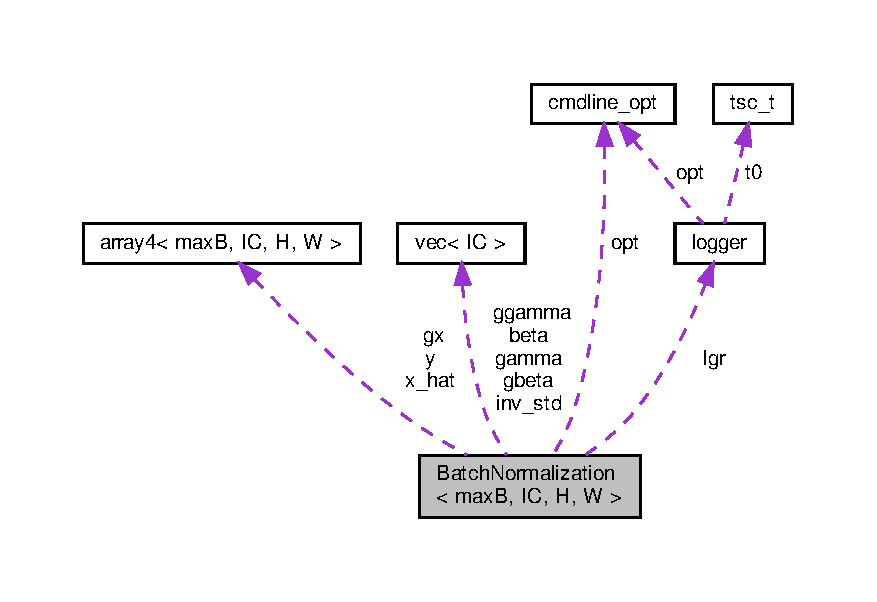
\includegraphics[width=350pt]{structBatchNormalization__coll__graph}
\end{center}
\end{figure}
\subsection*{Public Member Functions}
\begin{DoxyCompactItemize}
\item 
void \hyperlink{structBatchNormalization_aaf4e7179ded1be5c9284b9464cdde805}{init} (\hyperlink{structcmdline__opt}{cmdline\+\_\+opt} \hyperlink{structBatchNormalization_a9fb30ad9f94c91d4a4d4ab9d3801cba4}{opt}, \hyperlink{structlogger}{logger} $\ast$\hyperlink{structBatchNormalization_a160b18a54054d8afa967acc842dd9cf3}{lgr}, \hyperlink{structrnd__gen__t}{rnd\+\_\+gen\+\_\+t} \&rg)
\begin{DoxyCompactList}\small\item\em initialize \end{DoxyCompactList}\item 
\hyperlink{structBatchNormalization}{Batch\+Normalization}$<$ maxB, IC, H, W $>$ $\ast$ \hyperlink{structBatchNormalization_a328b3e1347324b4fec03662240f39aa5}{copy} ()
\begin{DoxyCompactList}\small\item\em make a copy of this \end{DoxyCompactList}\item 
void \hyperlink{structBatchNormalization_a05caf41d5a21914b07652d356fde7387}{set\+\_\+dev} (\hyperlink{structBatchNormalization}{Batch\+Normalization}$<$ maxB, IC, H, W $>$ $\ast$\hyperlink{structBatchNormalization_a86d66680b05689ca3df6297e3fd6598e}{dev})
\begin{DoxyCompactList}\small\item\em set the device pointer for this and all subobjects \end{DoxyCompactList}\item 
void \hyperlink{structBatchNormalization_a0d925e23b6e4d49e64319dd02d93b480}{make\+\_\+dev} ()
\begin{DoxyCompactList}\small\item\em if the algorithm is a gpu algorithm, allocate a device shadow of this object and set dev field of this and all subobjects. otherwise it sets all dev fields to null. \end{DoxyCompactList}\item 
void \hyperlink{structBatchNormalization_a3698340b540985a0cb1d5d2711fc8334}{del\+\_\+dev} ()
\begin{DoxyCompactList}\small\item\em if the algorithm is a gpu algorithm, dev field must not be null and deallocate it. \end{DoxyCompactList}\item 
\mbox{\Hypertarget{structBatchNormalization_a42df88ade175bae177a59b347dc52884}\label{structBatchNormalization_a42df88ade175bae177a59b347dc52884}} 
void \hyperlink{structBatchNormalization_a42df88ade175bae177a59b347dc52884}{to\+\_\+dev} ()
\begin{DoxyCompactList}\small\item\em if the algorithm is a gpu algorithm, dev field must not be null and send the host data to the device memory \end{DoxyCompactList}\item 
\mbox{\Hypertarget{structBatchNormalization_a4e7f098947f8d4896b1fe39e67263713}\label{structBatchNormalization_a4e7f098947f8d4896b1fe39e67263713}} 
void \hyperlink{structBatchNormalization_a4e7f098947f8d4896b1fe39e67263713}{to\+\_\+host} ()
\begin{DoxyCompactList}\small\item\em if the algorithm is a gpu algorithm, dev field must not be null and send the device data to the host memory \end{DoxyCompactList}\item 
\+\_\+\+\_\+device\+\_\+\+\_\+ \+\_\+\+\_\+host\+\_\+\+\_\+ void \hyperlink{structBatchNormalization_a757cb54212040fca8bc2465bbac26636}{update\+\_\+base} (\hyperlink{vgg__util_8h_a1082d08aaa761215ec83e7149f27ad16}{real} eta)
\begin{DoxyCompactList}\small\item\em the baseline (serial) implementation of update called both by cpu implementation (update\+\_\+cpu) and gpu implementation (update\+\_\+dev). the call sequence update -\/$>$ update\+\_\+cpu -\/$>$ update\+\_\+base on cpu and and is update -\/$>$ update\+\_\+gpu -\/$>$ update\+\_\+global -\/$>$ update\+\_\+dev -\/$>$ update\+\_\+base \end{DoxyCompactList}\item 
\+\_\+\+\_\+device\+\_\+\+\_\+ void \hyperlink{structBatchNormalization_a463e10e6b59905d8c1e9bcac3a17a126}{update\+\_\+dev} (\hyperlink{vgg__util_8h_a1082d08aaa761215ec83e7149f27ad16}{real} eta)
\begin{DoxyCompactList}\small\item\em the device function of update called from the global (non-\/member) function \end{DoxyCompactList}\item 
void \hyperlink{structBatchNormalization_a1e65c4b6e011da3e8176e56ccb83e453}{update\+\_\+gpu} (\hyperlink{vgg__util_8h_a1082d08aaa761215ec83e7149f27ad16}{real} eta)
\begin{DoxyCompactList}\small\item\em a gpu version of baseline code called from the entry function (update) \end{DoxyCompactList}\item 
void \hyperlink{structBatchNormalization_a223b6369246bad1525c2284a0285c581}{update\+\_\+cpu} (\hyperlink{vgg__util_8h_a1082d08aaa761215ec83e7149f27ad16}{real} eta)
\begin{DoxyCompactList}\small\item\em a cpu version of baseline code called from the entry function (update) \end{DoxyCompactList}\item 
void \hyperlink{structBatchNormalization_a71b4c3d0b5002d84ba2d74f47f7ab8d2}{update} (\hyperlink{vgg__util_8h_a1082d08aaa761215ec83e7149f27ad16}{real} eta)
\begin{DoxyCompactList}\small\item\em update weights of all sublayers with gradients that must have been computed \end{DoxyCompactList}\item 
\+\_\+\+\_\+device\+\_\+\+\_\+ \+\_\+\+\_\+host\+\_\+\+\_\+ \hyperlink{structvec}{vec}$<$ IC $>$ \hyperlink{structBatchNormalization_a0d4c799cedf33dae08d3b46f417c1ecf}{mean\+\_\+bij} (\hyperlink{structarray4}{array4}$<$ maxB, IC, H, W $>$ \&x)
\begin{DoxyCompactList}\small\item\em calc a mean of each input channel \end{DoxyCompactList}\item 
\+\_\+\+\_\+device\+\_\+\+\_\+ \+\_\+\+\_\+host\+\_\+\+\_\+ \hyperlink{structvec}{vec}$<$ IC $>$ \& \hyperlink{structBatchNormalization_a631234804d2a88d43655ab06ea4d5bfc}{inv\+\_\+std\+\_\+bij} (\hyperlink{structarray4}{array4}$<$ maxB, IC, H, W $>$ \&x, \hyperlink{structvec}{vec}$<$ IC $>$ \&mu)
\begin{DoxyCompactList}\small\item\em calc a standard deviation of each input channel \end{DoxyCompactList}\item 
\+\_\+\+\_\+device\+\_\+\+\_\+ \+\_\+\+\_\+host\+\_\+\+\_\+ void \hyperlink{structBatchNormalization_a95b82689b898e3e9940a98a0145eb6ca}{forward\+\_\+base} (\hyperlink{structarray4}{array4}$<$ maxB, IC, H, W $>$ \&x)
\begin{DoxyCompactList}\small\item\em the baseline (serial) implementation of forward called both by cpu implementation (forward\+\_\+cpu) and gpu implementation (forward\+\_\+dev). the call sequence forward -\/$>$ forward\+\_\+cpu -\/$>$ forward\+\_\+base on cpu and and is forward -\/$>$ forward\+\_\+gpu -\/$>$ forward\+\_\+global -\/$>$ forward\+\_\+dev -\/$>$ forward\+\_\+base \end{DoxyCompactList}\item 
\+\_\+\+\_\+device\+\_\+\+\_\+ void \hyperlink{structBatchNormalization_a5c35968b76ca1a166fe93aede17b53e8}{forward\+\_\+dev} (\hyperlink{structarray4}{array4}$<$ maxB, IC, H, W $>$ \&x)
\begin{DoxyCompactList}\small\item\em the device function of forward called from the global (non-\/member) function \end{DoxyCompactList}\item 
void \hyperlink{structBatchNormalization_a66c02d8d49ae80a8edd186024c04d42a}{forward\+\_\+gpu} (\hyperlink{structarray4}{array4}$<$ maxB, IC, H, W $>$ \&x)
\begin{DoxyCompactList}\small\item\em a gpu version of baseline code called from the entry function (forward) \end{DoxyCompactList}\item 
void \hyperlink{structBatchNormalization_a9490250c2e3469b619e76e5c913aa830}{forward\+\_\+cpu} (\hyperlink{structarray4}{array4}$<$ maxB, IC, H, W $>$ \&x)
\begin{DoxyCompactList}\small\item\em a cpu version of baseline code called from the entry function (forward) \end{DoxyCompactList}\item 
\hyperlink{structarray4}{array4}$<$ maxB, IC, H, W $>$ \& \hyperlink{structBatchNormalization_a315cda9d48dfa18a2f4f65ac7bb3b891}{forward} (\hyperlink{structarray4}{array4}$<$ maxB, IC, H, W $>$ \&x)
\begin{DoxyCompactList}\small\item\em calc the loss function of a mini-\/batch (x,t) \end{DoxyCompactList}\item 
\+\_\+\+\_\+device\+\_\+\+\_\+ \+\_\+\+\_\+host\+\_\+\+\_\+ void \hyperlink{structBatchNormalization_a0ef45335c50151f68de03d33b1d226ca}{backward\+\_\+base} (\hyperlink{structarray4}{array4}$<$ maxB, IC, H, W $>$ \&gy)
\begin{DoxyCompactList}\small\item\em the baseline (serial) implementation of backward called both by cpu implementation (backward\+\_\+cpu) and gpu implementation (backward\+\_\+dev). the call sequence backward -\/$>$ backward\+\_\+cpu -\/$>$ backward\+\_\+base on cpu and and is backward -\/$>$ backward\+\_\+gpu -\/$>$ backward\+\_\+global -\/$>$ backward\+\_\+dev -\/$>$ backward\+\_\+base \end{DoxyCompactList}\item 
\+\_\+\+\_\+device\+\_\+\+\_\+ void \hyperlink{structBatchNormalization_a3c96c56393798abdb00647aae73b197a}{backward\+\_\+dev} (\hyperlink{structarray4}{array4}$<$ maxB, IC, H, W $>$ \&gy)
\begin{DoxyCompactList}\small\item\em the device function of backward called from the global (non-\/member) function \end{DoxyCompactList}\item 
void \hyperlink{structBatchNormalization_a2a80a633ecc4a5ed378dd0ff70d275e1}{backward\+\_\+gpu} (\hyperlink{structarray4}{array4}$<$ maxB, IC, H, W $>$ \&gy)
\begin{DoxyCompactList}\small\item\em a gpu version of baseline code called from the entry function (backward) \end{DoxyCompactList}\item 
void \hyperlink{structBatchNormalization_af60d17f3a0af3a4fd8556a93eddcf7c9}{backward\+\_\+cpu} (\hyperlink{structarray4}{array4}$<$ maxB, IC, H, W $>$ \&gy)
\begin{DoxyCompactList}\small\item\em a cpu version of baseline code called from the entry function (backward) \end{DoxyCompactList}\item 
\hyperlink{structarray4}{array4}$<$ maxB, IC, H, W $>$ \& \hyperlink{structBatchNormalization_a3b6d987026effdc6c3a2c99e54ae58f9}{backward} (\hyperlink{structarray4}{array4}$<$ maxB, IC, H, W $>$ \&gy)
\begin{DoxyCompactList}\small\item\em calc the gradient of loss wrt the input (x) \end{DoxyCompactList}\item 
void \hyperlink{structBatchNormalization_acf65ad8948335d6a4ebff9ba2a0ab906}{rand\+\_\+grad} (\hyperlink{structrnd__gen__t}{rnd\+\_\+gen\+\_\+t} \&rg, \hyperlink{vgg__util_8h_a1082d08aaa761215ec83e7149f27ad16}{real} p, \hyperlink{vgg__util_8h_a1082d08aaa761215ec83e7149f27ad16}{real} q)
\begin{DoxyCompactList}\small\item\em randomly set all gradients to values between p and q \end{DoxyCompactList}\item 
void \hyperlink{structBatchNormalization_aeadf5127ff94fb3e53c30272e7346f0d}{set\+\_\+grad} (\hyperlink{structBatchNormalization}{Batch\+Normalization}$<$ maxB, IC, H, W $>$ \&o)
\begin{DoxyCompactList}\small\item\em set all gradients to gradients of another object \end{DoxyCompactList}\item 
\hyperlink{vgg__util_8h_a1082d08aaa761215ec83e7149f27ad16}{real} \hyperlink{structBatchNormalization_a377e27f39a4f1e26c952fcf12b362cb3}{gw\+\_\+dot\+\_\+gw} (\hyperlink{structBatchNormalization}{Batch\+Normalization}$<$ maxB, IC, H, W $>$ \&b)
\begin{DoxyCompactList}\small\item\em take the inner product of gradients \end{DoxyCompactList}\end{DoxyCompactItemize}
\subsection*{Public Attributes}
\begin{DoxyCompactItemize}
\item 
\hyperlink{structBatchNormalization}{Batch\+Normalization}$<$ maxB, IC, H, W $>$ $\ast$ \hyperlink{structBatchNormalization_a86d66680b05689ca3df6297e3fd6598e}{dev}
\item 
\hyperlink{structcmdline__opt}{cmdline\+\_\+opt} \hyperlink{structBatchNormalization_a9fb30ad9f94c91d4a4d4ab9d3801cba4}{opt}
\item 
\hyperlink{structlogger}{logger} $\ast$ \hyperlink{structBatchNormalization_a160b18a54054d8afa967acc842dd9cf3}{lgr}
\item 
\hyperlink{structvec}{vec}$<$ IC $>$ \hyperlink{structBatchNormalization_a19341c5df4950a9df17dc3ca2f2b9ecf}{gamma}
\item 
\hyperlink{structvec}{vec}$<$ IC $>$ \hyperlink{structBatchNormalization_a751b4044335ece13ce09f962168e8f1e}{beta}
\item 
\hyperlink{structarray4}{array4}$<$ maxB, IC, H, W $>$ \hyperlink{structBatchNormalization_ab0962f839e8eed605d7fb43fc2eb979d}{x\+\_\+hat}
\item 
\hyperlink{structvec}{vec}$<$ IC $>$ \hyperlink{structBatchNormalization_a32b254c9c4ceb4dc1c952d93851d120f}{inv\+\_\+std}
\item 
\hyperlink{structarray4}{array4}$<$ maxB, IC, H, W $>$ \hyperlink{structBatchNormalization_a1453d9955c9cb72c5316c98cb06d1867}{y}
\item 
\hyperlink{structvec}{vec}$<$ IC $>$ \hyperlink{structBatchNormalization_a050a1a786d6b10b0c0359214cfdb4fef}{ggamma}
\item 
\hyperlink{structvec}{vec}$<$ IC $>$ \hyperlink{structBatchNormalization_a881e8679992c8e0fb22c2e208e55e93d}{gbeta}
\item 
\hyperlink{structarray4}{array4}$<$ maxB, IC, H, W $>$ \hyperlink{structBatchNormalization_a916260aac816d659d876988c94666791}{gx}
\end{DoxyCompactItemize}


\subsection{Detailed Description}
\subsubsection*{template$<$idx\+\_\+t maxB, idx\+\_\+t IC, idx\+\_\+t H, idx\+\_\+t W$>$\newline
struct Batch\+Normalization$<$ max\+B, I\+C, H, W $>$}

batch normalization 


\begin{DoxyParams}{Parameters}
{\em (max\+B)} & the maximum number of images (batch size) \\
\hline
{\em (\+I\+C)} & the number of channels per input image (the original input has typically three channels for R\+GB. in hidden layers, it starts from 64 and goes up to 512 in the last hidden layer) \\
\hline
{\em (\+H)} & height of an image (32 for an input image, down to 1 in the last hidden layer) \\
\hline
{\em (\+W)} & width of an image (32 for an input image, down to 1 in the last hidden layer)\\
\hline
\end{DoxyParams}
this layer normalizes a batch of images 

\subsection{Member Function Documentation}
\mbox{\Hypertarget{structBatchNormalization_a3b6d987026effdc6c3a2c99e54ae58f9}\label{structBatchNormalization_a3b6d987026effdc6c3a2c99e54ae58f9}} 
\index{Batch\+Normalization@{Batch\+Normalization}!backward@{backward}}
\index{backward@{backward}!Batch\+Normalization@{Batch\+Normalization}}
\subsubsection{\texorpdfstring{backward()}{backward()}}
{\footnotesize\ttfamily template$<$idx\+\_\+t maxB, idx\+\_\+t IC, idx\+\_\+t H, idx\+\_\+t W$>$ \\
\hyperlink{structarray4}{array4}$<$maxB,IC,H,W$>$\& \hyperlink{structBatchNormalization}{Batch\+Normalization}$<$ maxB, IC, H, W $>$\+::backward (\begin{DoxyParamCaption}\item[{\hyperlink{structarray4}{array4}$<$ maxB, IC, H, W $>$ \&}]{gy }\end{DoxyParamCaption})\hspace{0.3cm}{\ttfamily [inline]}}



calc the gradient of loss wrt the input (x) 


\begin{DoxyParams}{Parameters}
{\em (gy)} & gradient of loss with respect to the output\\
\hline
\end{DoxyParams}
calc the gradient of loss wrt the input. along the way, it also calculates the gradient of loss wrt weights for all sublayers that have weights. since this is the entire network, gy is actually a vector whose components are all 1. (loss = sum of losses of each data). \begin{DoxySeeAlso}{See also}
\hyperlink{structBatchNormalization_a315cda9d48dfa18a2f4f65ac7bb3b891}{forward} 

\hyperlink{structBatchNormalization_a71b4c3d0b5002d84ba2d74f47f7ab8d2}{update} 
\end{DoxySeeAlso}
\mbox{\Hypertarget{structBatchNormalization_a0ef45335c50151f68de03d33b1d226ca}\label{structBatchNormalization_a0ef45335c50151f68de03d33b1d226ca}} 
\index{Batch\+Normalization@{Batch\+Normalization}!backward\+\_\+base@{backward\+\_\+base}}
\index{backward\+\_\+base@{backward\+\_\+base}!Batch\+Normalization@{Batch\+Normalization}}
\subsubsection{\texorpdfstring{backward\+\_\+base()}{backward\_base()}}
{\footnotesize\ttfamily template$<$idx\+\_\+t maxB, idx\+\_\+t IC, idx\+\_\+t H, idx\+\_\+t W$>$ \\
\+\_\+\+\_\+device\+\_\+\+\_\+ \+\_\+\+\_\+host\+\_\+\+\_\+ void \hyperlink{structBatchNormalization}{Batch\+Normalization}$<$ maxB, IC, H, W $>$\+::backward\+\_\+base (\begin{DoxyParamCaption}\item[{\hyperlink{structarray4}{array4}$<$ maxB, IC, H, W $>$ \&}]{gy }\end{DoxyParamCaption})\hspace{0.3cm}{\ttfamily [inline]}}



the baseline (serial) implementation of backward called both by cpu implementation (backward\+\_\+cpu) and gpu implementation (backward\+\_\+dev). the call sequence backward -\/$>$ backward\+\_\+cpu -\/$>$ backward\+\_\+base on cpu and and is backward -\/$>$ backward\+\_\+gpu -\/$>$ backward\+\_\+global -\/$>$ backward\+\_\+dev -\/$>$ backward\+\_\+base 


\begin{DoxyParams}{Parameters}
{\em (gy)} & the gradient of loss wrt y \\
\hline
\end{DoxyParams}
\begin{DoxySeeAlso}{See also}
\hyperlink{structBatchNormalization_a3b6d987026effdc6c3a2c99e54ae58f9}{backward} 

\hyperlink{structBatchNormalization_a2a80a633ecc4a5ed378dd0ff70d275e1}{backward\+\_\+gpu} 

\hyperlink{softmaxcrossentropy_8h_a47d56a9a23e08247b227f4aac17413e0}{backward\+\_\+global} 

\hyperlink{structBatchNormalization_a3c96c56393798abdb00647aae73b197a}{backward\+\_\+dev} 
\end{DoxySeeAlso}
\mbox{\Hypertarget{structBatchNormalization_af60d17f3a0af3a4fd8556a93eddcf7c9}\label{structBatchNormalization_af60d17f3a0af3a4fd8556a93eddcf7c9}} 
\index{Batch\+Normalization@{Batch\+Normalization}!backward\+\_\+cpu@{backward\+\_\+cpu}}
\index{backward\+\_\+cpu@{backward\+\_\+cpu}!Batch\+Normalization@{Batch\+Normalization}}
\subsubsection{\texorpdfstring{backward\+\_\+cpu()}{backward\_cpu()}}
{\footnotesize\ttfamily template$<$idx\+\_\+t maxB, idx\+\_\+t IC, idx\+\_\+t H, idx\+\_\+t W$>$ \\
void \hyperlink{structBatchNormalization}{Batch\+Normalization}$<$ maxB, IC, H, W $>$\+::backward\+\_\+cpu (\begin{DoxyParamCaption}\item[{\hyperlink{structarray4}{array4}$<$ maxB, IC, H, W $>$ \&}]{gy }\end{DoxyParamCaption})\hspace{0.3cm}{\ttfamily [inline]}}



a cpu version of baseline code called from the entry function (backward) 


\begin{DoxyParams}{Parameters}
{\em (gy)} & the gradient of loss wrt y \\
\hline
\end{DoxyParams}
\begin{DoxySeeAlso}{See also}
\hyperlink{structBatchNormalization_a3b6d987026effdc6c3a2c99e54ae58f9}{backward} 

\hyperlink{structBatchNormalization_a0ef45335c50151f68de03d33b1d226ca}{backward\+\_\+base} 
\end{DoxySeeAlso}
\mbox{\Hypertarget{structBatchNormalization_a3c96c56393798abdb00647aae73b197a}\label{structBatchNormalization_a3c96c56393798abdb00647aae73b197a}} 
\index{Batch\+Normalization@{Batch\+Normalization}!backward\+\_\+dev@{backward\+\_\+dev}}
\index{backward\+\_\+dev@{backward\+\_\+dev}!Batch\+Normalization@{Batch\+Normalization}}
\subsubsection{\texorpdfstring{backward\+\_\+dev()}{backward\_dev()}}
{\footnotesize\ttfamily template$<$idx\+\_\+t maxB, idx\+\_\+t IC, idx\+\_\+t H, idx\+\_\+t W$>$ \\
\+\_\+\+\_\+device\+\_\+\+\_\+ void \hyperlink{structBatchNormalization}{Batch\+Normalization}$<$ maxB, IC, H, W $>$\+::backward\+\_\+dev (\begin{DoxyParamCaption}\item[{\hyperlink{structarray4}{array4}$<$ maxB, IC, H, W $>$ \&}]{gy }\end{DoxyParamCaption})\hspace{0.3cm}{\ttfamily [inline]}}



the device function of backward called from the global (non-\/member) function 


\begin{DoxyParams}{Parameters}
{\em (gy)} & the gradient of loss wrt y \\
\hline
\end{DoxyParams}
\begin{DoxySeeAlso}{See also}
\hyperlink{structBatchNormalization_a3b6d987026effdc6c3a2c99e54ae58f9}{backward} 

\hyperlink{structBatchNormalization_a2a80a633ecc4a5ed378dd0ff70d275e1}{backward\+\_\+gpu} 

\hyperlink{softmaxcrossentropy_8h_a47d56a9a23e08247b227f4aac17413e0}{backward\+\_\+global} 

\hyperlink{structBatchNormalization_a0ef45335c50151f68de03d33b1d226ca}{backward\+\_\+base} 
\end{DoxySeeAlso}
\mbox{\Hypertarget{structBatchNormalization_a2a80a633ecc4a5ed378dd0ff70d275e1}\label{structBatchNormalization_a2a80a633ecc4a5ed378dd0ff70d275e1}} 
\index{Batch\+Normalization@{Batch\+Normalization}!backward\+\_\+gpu@{backward\+\_\+gpu}}
\index{backward\+\_\+gpu@{backward\+\_\+gpu}!Batch\+Normalization@{Batch\+Normalization}}
\subsubsection{\texorpdfstring{backward\+\_\+gpu()}{backward\_gpu()}}
{\footnotesize\ttfamily template$<$idx\+\_\+t maxB, idx\+\_\+t IC, idx\+\_\+t H, idx\+\_\+t W$>$ \\
void \hyperlink{structBatchNormalization}{Batch\+Normalization}$<$ maxB, IC, H, W $>$\+::backward\+\_\+gpu (\begin{DoxyParamCaption}\item[{\hyperlink{structarray4}{array4}$<$ maxB, IC, H, W $>$ \&}]{gy }\end{DoxyParamCaption})\hspace{0.3cm}{\ttfamily [inline]}}



a gpu version of baseline code called from the entry function (backward) 


\begin{DoxyParams}{Parameters}
{\em (gy)} & gradient of loss with respect to the output \\
\hline
\end{DoxyParams}
\begin{DoxySeeAlso}{See also}
\hyperlink{structBatchNormalization_a3b6d987026effdc6c3a2c99e54ae58f9}{backward} 

\hyperlink{softmaxcrossentropy_8h_a47d56a9a23e08247b227f4aac17413e0}{backward\+\_\+global} 

\hyperlink{structBatchNormalization_a3c96c56393798abdb00647aae73b197a}{backward\+\_\+dev} 

\hyperlink{structBatchNormalization_a0ef45335c50151f68de03d33b1d226ca}{backward\+\_\+base} 
\end{DoxySeeAlso}
\mbox{\Hypertarget{structBatchNormalization_a328b3e1347324b4fec03662240f39aa5}\label{structBatchNormalization_a328b3e1347324b4fec03662240f39aa5}} 
\index{Batch\+Normalization@{Batch\+Normalization}!copy@{copy}}
\index{copy@{copy}!Batch\+Normalization@{Batch\+Normalization}}
\subsubsection{\texorpdfstring{copy()}{copy()}}
{\footnotesize\ttfamily template$<$idx\+\_\+t maxB, idx\+\_\+t IC, idx\+\_\+t H, idx\+\_\+t W$>$ \\
\hyperlink{structBatchNormalization}{Batch\+Normalization}$<$maxB,IC,H,W$>$$\ast$ \hyperlink{structBatchNormalization}{Batch\+Normalization}$<$ maxB, IC, H, W $>$\+::copy (\begin{DoxyParamCaption}{ }\end{DoxyParamCaption})\hspace{0.3cm}{\ttfamily [inline]}}



make a copy of this 

if this object has a device pointer, the copy will have a device pointer too, but its contents are N\+OT copied \mbox{\Hypertarget{structBatchNormalization_a3698340b540985a0cb1d5d2711fc8334}\label{structBatchNormalization_a3698340b540985a0cb1d5d2711fc8334}} 
\index{Batch\+Normalization@{Batch\+Normalization}!del\+\_\+dev@{del\+\_\+dev}}
\index{del\+\_\+dev@{del\+\_\+dev}!Batch\+Normalization@{Batch\+Normalization}}
\subsubsection{\texorpdfstring{del\+\_\+dev()}{del\_dev()}}
{\footnotesize\ttfamily template$<$idx\+\_\+t maxB, idx\+\_\+t IC, idx\+\_\+t H, idx\+\_\+t W$>$ \\
void \hyperlink{structBatchNormalization}{Batch\+Normalization}$<$ maxB, IC, H, W $>$\+::del\+\_\+dev (\begin{DoxyParamCaption}{ }\end{DoxyParamCaption})\hspace{0.3cm}{\ttfamily [inline]}}



if the algorithm is a gpu algorithm, dev field must not be null and deallocate it. 

\begin{DoxySeeAlso}{See also}
\hyperlink{structBatchNormalization_a0d925e23b6e4d49e64319dd02d93b480}{make\+\_\+dev} 

\hyperlink{structBatchNormalization_a05caf41d5a21914b07652d356fde7387}{set\+\_\+dev} 
\end{DoxySeeAlso}
\mbox{\Hypertarget{structBatchNormalization_a315cda9d48dfa18a2f4f65ac7bb3b891}\label{structBatchNormalization_a315cda9d48dfa18a2f4f65ac7bb3b891}} 
\index{Batch\+Normalization@{Batch\+Normalization}!forward@{forward}}
\index{forward@{forward}!Batch\+Normalization@{Batch\+Normalization}}
\subsubsection{\texorpdfstring{forward()}{forward()}}
{\footnotesize\ttfamily template$<$idx\+\_\+t maxB, idx\+\_\+t IC, idx\+\_\+t H, idx\+\_\+t W$>$ \\
\hyperlink{structarray4}{array4}$<$maxB,IC,H,W$>$\& \hyperlink{structBatchNormalization}{Batch\+Normalization}$<$ maxB, IC, H, W $>$\+::forward (\begin{DoxyParamCaption}\item[{\hyperlink{structarray4}{array4}$<$ maxB, IC, H, W $>$ \&}]{x }\end{DoxyParamCaption})\hspace{0.3cm}{\ttfamily [inline]}}



calc the loss function of a mini-\/batch (x,t) 


\begin{DoxyParams}{Parameters}
{\em (x)} & input images \\
\hline
\end{DoxyParams}
\begin{DoxySeeAlso}{See also}
\hyperlink{structBatchNormalization_a3b6d987026effdc6c3a2c99e54ae58f9}{backward} 

\hyperlink{structBatchNormalization_a71b4c3d0b5002d84ba2d74f47f7ab8d2}{update} 
\end{DoxySeeAlso}
\mbox{\Hypertarget{structBatchNormalization_a95b82689b898e3e9940a98a0145eb6ca}\label{structBatchNormalization_a95b82689b898e3e9940a98a0145eb6ca}} 
\index{Batch\+Normalization@{Batch\+Normalization}!forward\+\_\+base@{forward\+\_\+base}}
\index{forward\+\_\+base@{forward\+\_\+base}!Batch\+Normalization@{Batch\+Normalization}}
\subsubsection{\texorpdfstring{forward\+\_\+base()}{forward\_base()}}
{\footnotesize\ttfamily template$<$idx\+\_\+t maxB, idx\+\_\+t IC, idx\+\_\+t H, idx\+\_\+t W$>$ \\
\+\_\+\+\_\+device\+\_\+\+\_\+ \+\_\+\+\_\+host\+\_\+\+\_\+ void \hyperlink{structBatchNormalization}{Batch\+Normalization}$<$ maxB, IC, H, W $>$\+::forward\+\_\+base (\begin{DoxyParamCaption}\item[{\hyperlink{structarray4}{array4}$<$ maxB, IC, H, W $>$ \&}]{x }\end{DoxyParamCaption})\hspace{0.3cm}{\ttfamily [inline]}}



the baseline (serial) implementation of forward called both by cpu implementation (forward\+\_\+cpu) and gpu implementation (forward\+\_\+dev). the call sequence forward -\/$>$ forward\+\_\+cpu -\/$>$ forward\+\_\+base on cpu and and is forward -\/$>$ forward\+\_\+gpu -\/$>$ forward\+\_\+global -\/$>$ forward\+\_\+dev -\/$>$ forward\+\_\+base 


\begin{DoxyParams}{Parameters}
{\em (x)} & input images \\
\hline
\end{DoxyParams}
\begin{DoxySeeAlso}{See also}
\hyperlink{structBatchNormalization_a315cda9d48dfa18a2f4f65ac7bb3b891}{forward} 

\hyperlink{structBatchNormalization_a66c02d8d49ae80a8edd186024c04d42a}{forward\+\_\+gpu} 

\hyperlink{softmaxcrossentropy_8h_a578aeeb166bd06e800d9b396eab48b35}{forward\+\_\+global} 

\hyperlink{structBatchNormalization_a5c35968b76ca1a166fe93aede17b53e8}{forward\+\_\+dev} 
\end{DoxySeeAlso}
\mbox{\Hypertarget{structBatchNormalization_a9490250c2e3469b619e76e5c913aa830}\label{structBatchNormalization_a9490250c2e3469b619e76e5c913aa830}} 
\index{Batch\+Normalization@{Batch\+Normalization}!forward\+\_\+cpu@{forward\+\_\+cpu}}
\index{forward\+\_\+cpu@{forward\+\_\+cpu}!Batch\+Normalization@{Batch\+Normalization}}
\subsubsection{\texorpdfstring{forward\+\_\+cpu()}{forward\_cpu()}}
{\footnotesize\ttfamily template$<$idx\+\_\+t maxB, idx\+\_\+t IC, idx\+\_\+t H, idx\+\_\+t W$>$ \\
void \hyperlink{structBatchNormalization}{Batch\+Normalization}$<$ maxB, IC, H, W $>$\+::forward\+\_\+cpu (\begin{DoxyParamCaption}\item[{\hyperlink{structarray4}{array4}$<$ maxB, IC, H, W $>$ \&}]{x }\end{DoxyParamCaption})\hspace{0.3cm}{\ttfamily [inline]}}



a cpu version of baseline code called from the entry function (forward) 


\begin{DoxyParams}{Parameters}
{\em (x)} & input images \\
\hline
\end{DoxyParams}
\begin{DoxySeeAlso}{See also}
\hyperlink{structBatchNormalization_a315cda9d48dfa18a2f4f65ac7bb3b891}{forward} 

\hyperlink{structBatchNormalization_a95b82689b898e3e9940a98a0145eb6ca}{forward\+\_\+base} 
\end{DoxySeeAlso}
\mbox{\Hypertarget{structBatchNormalization_a5c35968b76ca1a166fe93aede17b53e8}\label{structBatchNormalization_a5c35968b76ca1a166fe93aede17b53e8}} 
\index{Batch\+Normalization@{Batch\+Normalization}!forward\+\_\+dev@{forward\+\_\+dev}}
\index{forward\+\_\+dev@{forward\+\_\+dev}!Batch\+Normalization@{Batch\+Normalization}}
\subsubsection{\texorpdfstring{forward\+\_\+dev()}{forward\_dev()}}
{\footnotesize\ttfamily template$<$idx\+\_\+t maxB, idx\+\_\+t IC, idx\+\_\+t H, idx\+\_\+t W$>$ \\
\+\_\+\+\_\+device\+\_\+\+\_\+ void \hyperlink{structBatchNormalization}{Batch\+Normalization}$<$ maxB, IC, H, W $>$\+::forward\+\_\+dev (\begin{DoxyParamCaption}\item[{\hyperlink{structarray4}{array4}$<$ maxB, IC, H, W $>$ \&}]{x }\end{DoxyParamCaption})\hspace{0.3cm}{\ttfamily [inline]}}



the device function of forward called from the global (non-\/member) function 


\begin{DoxyParams}{Parameters}
{\em (x)} & input images \\
\hline
\end{DoxyParams}
\begin{DoxySeeAlso}{See also}
\hyperlink{structBatchNormalization_a315cda9d48dfa18a2f4f65ac7bb3b891}{forward} 

\hyperlink{structBatchNormalization_a66c02d8d49ae80a8edd186024c04d42a}{forward\+\_\+gpu} 

\hyperlink{softmaxcrossentropy_8h_a578aeeb166bd06e800d9b396eab48b35}{forward\+\_\+global} 

\hyperlink{structBatchNormalization_a95b82689b898e3e9940a98a0145eb6ca}{forward\+\_\+base} 
\end{DoxySeeAlso}
\mbox{\Hypertarget{structBatchNormalization_a66c02d8d49ae80a8edd186024c04d42a}\label{structBatchNormalization_a66c02d8d49ae80a8edd186024c04d42a}} 
\index{Batch\+Normalization@{Batch\+Normalization}!forward\+\_\+gpu@{forward\+\_\+gpu}}
\index{forward\+\_\+gpu@{forward\+\_\+gpu}!Batch\+Normalization@{Batch\+Normalization}}
\subsubsection{\texorpdfstring{forward\+\_\+gpu()}{forward\_gpu()}}
{\footnotesize\ttfamily template$<$idx\+\_\+t maxB, idx\+\_\+t IC, idx\+\_\+t H, idx\+\_\+t W$>$ \\
void \hyperlink{structBatchNormalization}{Batch\+Normalization}$<$ maxB, IC, H, W $>$\+::forward\+\_\+gpu (\begin{DoxyParamCaption}\item[{\hyperlink{structarray4}{array4}$<$ maxB, IC, H, W $>$ \&}]{x }\end{DoxyParamCaption})\hspace{0.3cm}{\ttfamily [inline]}}



a gpu version of baseline code called from the entry function (forward) 


\begin{DoxyParams}{Parameters}
{\em (x)} & input images \\
\hline
\end{DoxyParams}
\begin{DoxySeeAlso}{See also}
\hyperlink{structBatchNormalization_a315cda9d48dfa18a2f4f65ac7bb3b891}{forward} 

\hyperlink{softmaxcrossentropy_8h_a578aeeb166bd06e800d9b396eab48b35}{forward\+\_\+global} 

\hyperlink{structBatchNormalization_a5c35968b76ca1a166fe93aede17b53e8}{forward\+\_\+dev} 

\hyperlink{structBatchNormalization_a95b82689b898e3e9940a98a0145eb6ca}{forward\+\_\+base} 
\end{DoxySeeAlso}
\mbox{\Hypertarget{structBatchNormalization_a377e27f39a4f1e26c952fcf12b362cb3}\label{structBatchNormalization_a377e27f39a4f1e26c952fcf12b362cb3}} 
\index{Batch\+Normalization@{Batch\+Normalization}!gw\+\_\+dot\+\_\+gw@{gw\+\_\+dot\+\_\+gw}}
\index{gw\+\_\+dot\+\_\+gw@{gw\+\_\+dot\+\_\+gw}!Batch\+Normalization@{Batch\+Normalization}}
\subsubsection{\texorpdfstring{gw\+\_\+dot\+\_\+gw()}{gw\_dot\_gw()}}
{\footnotesize\ttfamily template$<$idx\+\_\+t maxB, idx\+\_\+t IC, idx\+\_\+t H, idx\+\_\+t W$>$ \\
\hyperlink{vgg__util_8h_a1082d08aaa761215ec83e7149f27ad16}{real} \hyperlink{structBatchNormalization}{Batch\+Normalization}$<$ maxB, IC, H, W $>$\+::gw\+\_\+dot\+\_\+gw (\begin{DoxyParamCaption}\item[{\hyperlink{structBatchNormalization}{Batch\+Normalization}$<$ maxB, IC, H, W $>$ \&}]{b }\end{DoxyParamCaption})\hspace{0.3cm}{\ttfamily [inline]}}



take the inner product of gradients 


\begin{DoxyParams}{Parameters}
{\em (b)} & the object to take the inner product with\\
\hline
\end{DoxyParams}
take the inner product of this object\textquotesingle{}s gradients and b\textquotesingle{}s gradients \mbox{\Hypertarget{structBatchNormalization_aaf4e7179ded1be5c9284b9464cdde805}\label{structBatchNormalization_aaf4e7179ded1be5c9284b9464cdde805}} 
\index{Batch\+Normalization@{Batch\+Normalization}!init@{init}}
\index{init@{init}!Batch\+Normalization@{Batch\+Normalization}}
\subsubsection{\texorpdfstring{init()}{init()}}
{\footnotesize\ttfamily template$<$idx\+\_\+t maxB, idx\+\_\+t IC, idx\+\_\+t H, idx\+\_\+t W$>$ \\
void \hyperlink{structBatchNormalization}{Batch\+Normalization}$<$ maxB, IC, H, W $>$\+::init (\begin{DoxyParamCaption}\item[{\hyperlink{structcmdline__opt}{cmdline\+\_\+opt}}]{opt,  }\item[{\hyperlink{structlogger}{logger} $\ast$}]{lgr,  }\item[{\hyperlink{structrnd__gen__t}{rnd\+\_\+gen\+\_\+t} \&}]{rg }\end{DoxyParamCaption})\hspace{0.3cm}{\ttfamily [inline]}}



initialize 


\begin{DoxyParams}{Parameters}
{\em (opt)} & command line options \\
\hline
{\em (lgr)} & logger \\
\hline
{\em (rg)} & random number generator for initializing weights \\
\hline
\end{DoxyParams}
\mbox{\Hypertarget{structBatchNormalization_a631234804d2a88d43655ab06ea4d5bfc}\label{structBatchNormalization_a631234804d2a88d43655ab06ea4d5bfc}} 
\index{Batch\+Normalization@{Batch\+Normalization}!inv\+\_\+std\+\_\+bij@{inv\+\_\+std\+\_\+bij}}
\index{inv\+\_\+std\+\_\+bij@{inv\+\_\+std\+\_\+bij}!Batch\+Normalization@{Batch\+Normalization}}
\subsubsection{\texorpdfstring{inv\+\_\+std\+\_\+bij()}{inv\_std\_bij()}}
{\footnotesize\ttfamily template$<$idx\+\_\+t maxB, idx\+\_\+t IC, idx\+\_\+t H, idx\+\_\+t W$>$ \\
\+\_\+\+\_\+device\+\_\+\+\_\+ \+\_\+\+\_\+host\+\_\+\+\_\+ \hyperlink{structvec}{vec}$<$IC$>$\& \hyperlink{structBatchNormalization}{Batch\+Normalization}$<$ maxB, IC, H, W $>$\+::inv\+\_\+std\+\_\+bij (\begin{DoxyParamCaption}\item[{\hyperlink{structarray4}{array4}$<$ maxB, IC, H, W $>$ \&}]{x,  }\item[{\hyperlink{structvec}{vec}$<$ IC $>$ \&}]{mu }\end{DoxyParamCaption})\hspace{0.3cm}{\ttfamily [inline]}}



calc a standard deviation of each input channel 


\begin{DoxyParams}{Parameters}
{\em (x)} & input images \\
\hline
{\em (mu)} & mean \\
\hline
\end{DoxyParams}
\begin{DoxySeeAlso}{See also}
\hyperlink{structBatchNormalization_a315cda9d48dfa18a2f4f65ac7bb3b891}{forward} 

\hyperlink{structBatchNormalization_a3b6d987026effdc6c3a2c99e54ae58f9}{backward}
\end{DoxySeeAlso}
this is an auxiliary function called from forward. inv\+\_\+std(i) = 1 / sqrt(standard deviation of pixel values over all pixels of all images in layer i) \mbox{\Hypertarget{structBatchNormalization_a0d925e23b6e4d49e64319dd02d93b480}\label{structBatchNormalization_a0d925e23b6e4d49e64319dd02d93b480}} 
\index{Batch\+Normalization@{Batch\+Normalization}!make\+\_\+dev@{make\+\_\+dev}}
\index{make\+\_\+dev@{make\+\_\+dev}!Batch\+Normalization@{Batch\+Normalization}}
\subsubsection{\texorpdfstring{make\+\_\+dev()}{make\_dev()}}
{\footnotesize\ttfamily template$<$idx\+\_\+t maxB, idx\+\_\+t IC, idx\+\_\+t H, idx\+\_\+t W$>$ \\
void \hyperlink{structBatchNormalization}{Batch\+Normalization}$<$ maxB, IC, H, W $>$\+::make\+\_\+dev (\begin{DoxyParamCaption}{ }\end{DoxyParamCaption})\hspace{0.3cm}{\ttfamily [inline]}}



if the algorithm is a gpu algorithm, allocate a device shadow of this object and set dev field of this and all subobjects. otherwise it sets all dev fields to null. 

\begin{DoxySeeAlso}{See also}
\hyperlink{structBatchNormalization_a05caf41d5a21914b07652d356fde7387}{set\+\_\+dev} 

\hyperlink{structBatchNormalization_a3698340b540985a0cb1d5d2711fc8334}{del\+\_\+dev} 
\end{DoxySeeAlso}
\mbox{\Hypertarget{structBatchNormalization_a0d4c799cedf33dae08d3b46f417c1ecf}\label{structBatchNormalization_a0d4c799cedf33dae08d3b46f417c1ecf}} 
\index{Batch\+Normalization@{Batch\+Normalization}!mean\+\_\+bij@{mean\+\_\+bij}}
\index{mean\+\_\+bij@{mean\+\_\+bij}!Batch\+Normalization@{Batch\+Normalization}}
\subsubsection{\texorpdfstring{mean\+\_\+bij()}{mean\_bij()}}
{\footnotesize\ttfamily template$<$idx\+\_\+t maxB, idx\+\_\+t IC, idx\+\_\+t H, idx\+\_\+t W$>$ \\
\+\_\+\+\_\+device\+\_\+\+\_\+ \+\_\+\+\_\+host\+\_\+\+\_\+ \hyperlink{structvec}{vec}$<$IC$>$ \hyperlink{structBatchNormalization}{Batch\+Normalization}$<$ maxB, IC, H, W $>$\+::mean\+\_\+bij (\begin{DoxyParamCaption}\item[{\hyperlink{structarray4}{array4}$<$ maxB, IC, H, W $>$ \&}]{x }\end{DoxyParamCaption})\hspace{0.3cm}{\ttfamily [inline]}}



calc a mean of each input channel 


\begin{DoxyParams}{Parameters}
{\em (x)} & input images \\
\hline
\end{DoxyParams}
\begin{DoxySeeAlso}{See also}
\hyperlink{structBatchNormalization_a315cda9d48dfa18a2f4f65ac7bb3b891}{forward} 

\hyperlink{structBatchNormalization_a3b6d987026effdc6c3a2c99e54ae58f9}{backward}
\end{DoxySeeAlso}
this is an auxiliary function called from forward. mean(i) = average of pixel values over all pixels of all images in layer i \mbox{\Hypertarget{structBatchNormalization_acf65ad8948335d6a4ebff9ba2a0ab906}\label{structBatchNormalization_acf65ad8948335d6a4ebff9ba2a0ab906}} 
\index{Batch\+Normalization@{Batch\+Normalization}!rand\+\_\+grad@{rand\+\_\+grad}}
\index{rand\+\_\+grad@{rand\+\_\+grad}!Batch\+Normalization@{Batch\+Normalization}}
\subsubsection{\texorpdfstring{rand\+\_\+grad()}{rand\_grad()}}
{\footnotesize\ttfamily template$<$idx\+\_\+t maxB, idx\+\_\+t IC, idx\+\_\+t H, idx\+\_\+t W$>$ \\
void \hyperlink{structBatchNormalization}{Batch\+Normalization}$<$ maxB, IC, H, W $>$\+::rand\+\_\+grad (\begin{DoxyParamCaption}\item[{\hyperlink{structrnd__gen__t}{rnd\+\_\+gen\+\_\+t} \&}]{rg,  }\item[{\hyperlink{vgg__util_8h_a1082d08aaa761215ec83e7149f27ad16}{real}}]{p,  }\item[{\hyperlink{vgg__util_8h_a1082d08aaa761215ec83e7149f27ad16}{real}}]{q }\end{DoxyParamCaption})\hspace{0.3cm}{\ttfamily [inline]}}



randomly set all gradients to values between p and q 


\begin{DoxyParams}{Parameters}
{\em (rg)} & random number generator \\
\hline
{\em (p)} & minimum value of a component \\
\hline
{\em (q)} & maximum value of a component \\
\hline
\end{DoxyParams}
\mbox{\Hypertarget{structBatchNormalization_a05caf41d5a21914b07652d356fde7387}\label{structBatchNormalization_a05caf41d5a21914b07652d356fde7387}} 
\index{Batch\+Normalization@{Batch\+Normalization}!set\+\_\+dev@{set\+\_\+dev}}
\index{set\+\_\+dev@{set\+\_\+dev}!Batch\+Normalization@{Batch\+Normalization}}
\subsubsection{\texorpdfstring{set\+\_\+dev()}{set\_dev()}}
{\footnotesize\ttfamily template$<$idx\+\_\+t maxB, idx\+\_\+t IC, idx\+\_\+t H, idx\+\_\+t W$>$ \\
void \hyperlink{structBatchNormalization}{Batch\+Normalization}$<$ maxB, IC, H, W $>$\+::set\+\_\+dev (\begin{DoxyParamCaption}\item[{\hyperlink{structBatchNormalization}{Batch\+Normalization}$<$ maxB, IC, H, W $>$ $\ast$}]{dev }\end{DoxyParamCaption})\hspace{0.3cm}{\ttfamily [inline]}}



set the device pointer for this and all subobjects 


\begin{DoxyParams}{Parameters}
{\em (dev)} & a device memory or null \\
\hline
\end{DoxyParams}
\begin{DoxySeeAlso}{See also}
\hyperlink{structBatchNormalization_a0d925e23b6e4d49e64319dd02d93b480}{make\+\_\+dev} 

\hyperlink{structBatchNormalization_a3698340b540985a0cb1d5d2711fc8334}{del\+\_\+dev}
\end{DoxySeeAlso}
if dev is not null, dev fields of all subojects point to the corresponding subjects in the device memory. if dev is not null, all dev fields become null. \mbox{\Hypertarget{structBatchNormalization_aeadf5127ff94fb3e53c30272e7346f0d}\label{structBatchNormalization_aeadf5127ff94fb3e53c30272e7346f0d}} 
\index{Batch\+Normalization@{Batch\+Normalization}!set\+\_\+grad@{set\+\_\+grad}}
\index{set\+\_\+grad@{set\+\_\+grad}!Batch\+Normalization@{Batch\+Normalization}}
\subsubsection{\texorpdfstring{set\+\_\+grad()}{set\_grad()}}
{\footnotesize\ttfamily template$<$idx\+\_\+t maxB, idx\+\_\+t IC, idx\+\_\+t H, idx\+\_\+t W$>$ \\
void \hyperlink{structBatchNormalization}{Batch\+Normalization}$<$ maxB, IC, H, W $>$\+::set\+\_\+grad (\begin{DoxyParamCaption}\item[{\hyperlink{structBatchNormalization}{Batch\+Normalization}$<$ maxB, IC, H, W $>$ \&}]{o }\end{DoxyParamCaption})\hspace{0.3cm}{\ttfamily [inline]}}



set all gradients to gradients of another object 


\begin{DoxyParams}{Parameters}
{\em (o)} & the object from which gradients get copied\\
\hline
\end{DoxyParams}
transfer gradients of o to this object \mbox{\Hypertarget{structBatchNormalization_a71b4c3d0b5002d84ba2d74f47f7ab8d2}\label{structBatchNormalization_a71b4c3d0b5002d84ba2d74f47f7ab8d2}} 
\index{Batch\+Normalization@{Batch\+Normalization}!update@{update}}
\index{update@{update}!Batch\+Normalization@{Batch\+Normalization}}
\subsubsection{\texorpdfstring{update()}{update()}}
{\footnotesize\ttfamily template$<$idx\+\_\+t maxB, idx\+\_\+t IC, idx\+\_\+t H, idx\+\_\+t W$>$ \\
void \hyperlink{structBatchNormalization}{Batch\+Normalization}$<$ maxB, IC, H, W $>$\+::update (\begin{DoxyParamCaption}\item[{\hyperlink{vgg__util_8h_a1082d08aaa761215ec83e7149f27ad16}{real}}]{eta }\end{DoxyParamCaption})\hspace{0.3cm}{\ttfamily [inline]}}



update weights of all sublayers with gradients that must have been computed 


\begin{DoxyParams}{Parameters}
{\em (eta)} & the learning rate \\
\hline
\end{DoxyParams}
\begin{DoxySeeAlso}{See also}
\hyperlink{structBatchNormalization_a315cda9d48dfa18a2f4f65ac7bb3b891}{forward} 

\hyperlink{structBatchNormalization_a3b6d987026effdc6c3a2c99e54ae58f9}{backward} 
\end{DoxySeeAlso}
\mbox{\Hypertarget{structBatchNormalization_a757cb54212040fca8bc2465bbac26636}\label{structBatchNormalization_a757cb54212040fca8bc2465bbac26636}} 
\index{Batch\+Normalization@{Batch\+Normalization}!update\+\_\+base@{update\+\_\+base}}
\index{update\+\_\+base@{update\+\_\+base}!Batch\+Normalization@{Batch\+Normalization}}
\subsubsection{\texorpdfstring{update\+\_\+base()}{update\_base()}}
{\footnotesize\ttfamily template$<$idx\+\_\+t maxB, idx\+\_\+t IC, idx\+\_\+t H, idx\+\_\+t W$>$ \\
\+\_\+\+\_\+device\+\_\+\+\_\+ \+\_\+\+\_\+host\+\_\+\+\_\+ void \hyperlink{structBatchNormalization}{Batch\+Normalization}$<$ maxB, IC, H, W $>$\+::update\+\_\+base (\begin{DoxyParamCaption}\item[{\hyperlink{vgg__util_8h_a1082d08aaa761215ec83e7149f27ad16}{real}}]{eta }\end{DoxyParamCaption})\hspace{0.3cm}{\ttfamily [inline]}}



the baseline (serial) implementation of update called both by cpu implementation (update\+\_\+cpu) and gpu implementation (update\+\_\+dev). the call sequence update -\/$>$ update\+\_\+cpu -\/$>$ update\+\_\+base on cpu and and is update -\/$>$ update\+\_\+gpu -\/$>$ update\+\_\+global -\/$>$ update\+\_\+dev -\/$>$ update\+\_\+base 


\begin{DoxyParams}{Parameters}
{\em (eta)} & the learning rate \\
\hline
\end{DoxyParams}
\begin{DoxySeeAlso}{See also}
\hyperlink{structBatchNormalization_a71b4c3d0b5002d84ba2d74f47f7ab8d2}{update} 

\hyperlink{structBatchNormalization_a1e65c4b6e011da3e8176e56ccb83e453}{update\+\_\+gpu} 

\hyperlink{linear_8h_a810703be28422bb9483665cbdbafd968}{update\+\_\+global} 

\hyperlink{structBatchNormalization_a463e10e6b59905d8c1e9bcac3a17a126}{update\+\_\+dev} 
\end{DoxySeeAlso}
\mbox{\Hypertarget{structBatchNormalization_a223b6369246bad1525c2284a0285c581}\label{structBatchNormalization_a223b6369246bad1525c2284a0285c581}} 
\index{Batch\+Normalization@{Batch\+Normalization}!update\+\_\+cpu@{update\+\_\+cpu}}
\index{update\+\_\+cpu@{update\+\_\+cpu}!Batch\+Normalization@{Batch\+Normalization}}
\subsubsection{\texorpdfstring{update\+\_\+cpu()}{update\_cpu()}}
{\footnotesize\ttfamily template$<$idx\+\_\+t maxB, idx\+\_\+t IC, idx\+\_\+t H, idx\+\_\+t W$>$ \\
void \hyperlink{structBatchNormalization}{Batch\+Normalization}$<$ maxB, IC, H, W $>$\+::update\+\_\+cpu (\begin{DoxyParamCaption}\item[{\hyperlink{vgg__util_8h_a1082d08aaa761215ec83e7149f27ad16}{real}}]{eta }\end{DoxyParamCaption})\hspace{0.3cm}{\ttfamily [inline]}}



a cpu version of baseline code called from the entry function (update) 


\begin{DoxyParams}{Parameters}
{\em (eta)} & the learning rate \\
\hline
\end{DoxyParams}
\begin{DoxySeeAlso}{See also}
\hyperlink{structBatchNormalization_a71b4c3d0b5002d84ba2d74f47f7ab8d2}{update} 

\hyperlink{structBatchNormalization_a757cb54212040fca8bc2465bbac26636}{update\+\_\+base} 
\end{DoxySeeAlso}
\mbox{\Hypertarget{structBatchNormalization_a463e10e6b59905d8c1e9bcac3a17a126}\label{structBatchNormalization_a463e10e6b59905d8c1e9bcac3a17a126}} 
\index{Batch\+Normalization@{Batch\+Normalization}!update\+\_\+dev@{update\+\_\+dev}}
\index{update\+\_\+dev@{update\+\_\+dev}!Batch\+Normalization@{Batch\+Normalization}}
\subsubsection{\texorpdfstring{update\+\_\+dev()}{update\_dev()}}
{\footnotesize\ttfamily template$<$idx\+\_\+t maxB, idx\+\_\+t IC, idx\+\_\+t H, idx\+\_\+t W$>$ \\
\+\_\+\+\_\+device\+\_\+\+\_\+ void \hyperlink{structBatchNormalization}{Batch\+Normalization}$<$ maxB, IC, H, W $>$\+::update\+\_\+dev (\begin{DoxyParamCaption}\item[{\hyperlink{vgg__util_8h_a1082d08aaa761215ec83e7149f27ad16}{real}}]{eta }\end{DoxyParamCaption})\hspace{0.3cm}{\ttfamily [inline]}}



the device function of update called from the global (non-\/member) function 


\begin{DoxyParams}{Parameters}
{\em (eta)} & the learning rate \\
\hline
\end{DoxyParams}
\begin{DoxySeeAlso}{See also}
\hyperlink{structBatchNormalization_a71b4c3d0b5002d84ba2d74f47f7ab8d2}{update} 

\hyperlink{structBatchNormalization_a1e65c4b6e011da3e8176e56ccb83e453}{update\+\_\+gpu} 

\hyperlink{linear_8h_a810703be28422bb9483665cbdbafd968}{update\+\_\+global} 

\hyperlink{structBatchNormalization_a757cb54212040fca8bc2465bbac26636}{update\+\_\+base} 
\end{DoxySeeAlso}
\mbox{\Hypertarget{structBatchNormalization_a1e65c4b6e011da3e8176e56ccb83e453}\label{structBatchNormalization_a1e65c4b6e011da3e8176e56ccb83e453}} 
\index{Batch\+Normalization@{Batch\+Normalization}!update\+\_\+gpu@{update\+\_\+gpu}}
\index{update\+\_\+gpu@{update\+\_\+gpu}!Batch\+Normalization@{Batch\+Normalization}}
\subsubsection{\texorpdfstring{update\+\_\+gpu()}{update\_gpu()}}
{\footnotesize\ttfamily template$<$idx\+\_\+t maxB, idx\+\_\+t IC, idx\+\_\+t H, idx\+\_\+t W$>$ \\
void \hyperlink{structBatchNormalization}{Batch\+Normalization}$<$ maxB, IC, H, W $>$\+::update\+\_\+gpu (\begin{DoxyParamCaption}\item[{\hyperlink{vgg__util_8h_a1082d08aaa761215ec83e7149f27ad16}{real}}]{eta }\end{DoxyParamCaption})\hspace{0.3cm}{\ttfamily [inline]}}



a gpu version of baseline code called from the entry function (update) 


\begin{DoxyParams}{Parameters}
{\em (eta)} & the learning rate \\
\hline
\end{DoxyParams}
\begin{DoxySeeAlso}{See also}
\hyperlink{structBatchNormalization_a71b4c3d0b5002d84ba2d74f47f7ab8d2}{update} 

\hyperlink{linear_8h_a810703be28422bb9483665cbdbafd968}{update\+\_\+global} 

\hyperlink{structBatchNormalization_a463e10e6b59905d8c1e9bcac3a17a126}{update\+\_\+dev} 

\hyperlink{structBatchNormalization_a757cb54212040fca8bc2465bbac26636}{update\+\_\+base} 
\end{DoxySeeAlso}


\subsection{Member Data Documentation}
\mbox{\Hypertarget{structBatchNormalization_a751b4044335ece13ce09f962168e8f1e}\label{structBatchNormalization_a751b4044335ece13ce09f962168e8f1e}} 
\index{Batch\+Normalization@{Batch\+Normalization}!beta@{beta}}
\index{beta@{beta}!Batch\+Normalization@{Batch\+Normalization}}
\subsubsection{\texorpdfstring{beta}{beta}}
{\footnotesize\ttfamily template$<$idx\+\_\+t maxB, idx\+\_\+t IC, idx\+\_\+t H, idx\+\_\+t W$>$ \\
\hyperlink{structvec}{vec}$<$IC$>$ \hyperlink{structBatchNormalization}{Batch\+Normalization}$<$ maxB, IC, H, W $>$\+::beta}

beta parameter \mbox{\Hypertarget{structBatchNormalization_a86d66680b05689ca3df6297e3fd6598e}\label{structBatchNormalization_a86d66680b05689ca3df6297e3fd6598e}} 
\index{Batch\+Normalization@{Batch\+Normalization}!dev@{dev}}
\index{dev@{dev}!Batch\+Normalization@{Batch\+Normalization}}
\subsubsection{\texorpdfstring{dev}{dev}}
{\footnotesize\ttfamily template$<$idx\+\_\+t maxB, idx\+\_\+t IC, idx\+\_\+t H, idx\+\_\+t W$>$ \\
\hyperlink{structBatchNormalization}{Batch\+Normalization}$<$maxB,IC,H,W$>$$\ast$ \hyperlink{structBatchNormalization}{Batch\+Normalization}$<$ maxB, IC, H, W $>$\+::dev}

device shadow \mbox{\Hypertarget{structBatchNormalization_a19341c5df4950a9df17dc3ca2f2b9ecf}\label{structBatchNormalization_a19341c5df4950a9df17dc3ca2f2b9ecf}} 
\index{Batch\+Normalization@{Batch\+Normalization}!gamma@{gamma}}
\index{gamma@{gamma}!Batch\+Normalization@{Batch\+Normalization}}
\subsubsection{\texorpdfstring{gamma}{gamma}}
{\footnotesize\ttfamily template$<$idx\+\_\+t maxB, idx\+\_\+t IC, idx\+\_\+t H, idx\+\_\+t W$>$ \\
\hyperlink{structvec}{vec}$<$IC$>$ \hyperlink{structBatchNormalization}{Batch\+Normalization}$<$ maxB, IC, H, W $>$\+::gamma}

gamma parameter \mbox{\Hypertarget{structBatchNormalization_a881e8679992c8e0fb22c2e208e55e93d}\label{structBatchNormalization_a881e8679992c8e0fb22c2e208e55e93d}} 
\index{Batch\+Normalization@{Batch\+Normalization}!gbeta@{gbeta}}
\index{gbeta@{gbeta}!Batch\+Normalization@{Batch\+Normalization}}
\subsubsection{\texorpdfstring{gbeta}{gbeta}}
{\footnotesize\ttfamily template$<$idx\+\_\+t maxB, idx\+\_\+t IC, idx\+\_\+t H, idx\+\_\+t W$>$ \\
\hyperlink{structvec}{vec}$<$IC$>$ \hyperlink{structBatchNormalization}{Batch\+Normalization}$<$ maxB, IC, H, W $>$\+::gbeta}

gradient of loss wrt beta \mbox{\Hypertarget{structBatchNormalization_a050a1a786d6b10b0c0359214cfdb4fef}\label{structBatchNormalization_a050a1a786d6b10b0c0359214cfdb4fef}} 
\index{Batch\+Normalization@{Batch\+Normalization}!ggamma@{ggamma}}
\index{ggamma@{ggamma}!Batch\+Normalization@{Batch\+Normalization}}
\subsubsection{\texorpdfstring{ggamma}{ggamma}}
{\footnotesize\ttfamily template$<$idx\+\_\+t maxB, idx\+\_\+t IC, idx\+\_\+t H, idx\+\_\+t W$>$ \\
\hyperlink{structvec}{vec}$<$IC$>$ \hyperlink{structBatchNormalization}{Batch\+Normalization}$<$ maxB, IC, H, W $>$\+::ggamma}

gradient of loss wrt gamma \mbox{\Hypertarget{structBatchNormalization_a916260aac816d659d876988c94666791}\label{structBatchNormalization_a916260aac816d659d876988c94666791}} 
\index{Batch\+Normalization@{Batch\+Normalization}!gx@{gx}}
\index{gx@{gx}!Batch\+Normalization@{Batch\+Normalization}}
\subsubsection{\texorpdfstring{gx}{gx}}
{\footnotesize\ttfamily template$<$idx\+\_\+t maxB, idx\+\_\+t IC, idx\+\_\+t H, idx\+\_\+t W$>$ \\
\hyperlink{structarray4}{array4}$<$maxB,IC,H,W$>$ \hyperlink{structBatchNormalization}{Batch\+Normalization}$<$ maxB, IC, H, W $>$\+::gx}

gradient of loss wrt x \mbox{\Hypertarget{structBatchNormalization_a32b254c9c4ceb4dc1c952d93851d120f}\label{structBatchNormalization_a32b254c9c4ceb4dc1c952d93851d120f}} 
\index{Batch\+Normalization@{Batch\+Normalization}!inv\+\_\+std@{inv\+\_\+std}}
\index{inv\+\_\+std@{inv\+\_\+std}!Batch\+Normalization@{Batch\+Normalization}}
\subsubsection{\texorpdfstring{inv\+\_\+std}{inv\_std}}
{\footnotesize\ttfamily template$<$idx\+\_\+t maxB, idx\+\_\+t IC, idx\+\_\+t H, idx\+\_\+t W$>$ \\
\hyperlink{structvec}{vec}$<$IC$>$ \hyperlink{structBatchNormalization}{Batch\+Normalization}$<$ maxB, IC, H, W $>$\+::inv\+\_\+std}

inverse of standard deviation \mbox{\Hypertarget{structBatchNormalization_a160b18a54054d8afa967acc842dd9cf3}\label{structBatchNormalization_a160b18a54054d8afa967acc842dd9cf3}} 
\index{Batch\+Normalization@{Batch\+Normalization}!lgr@{lgr}}
\index{lgr@{lgr}!Batch\+Normalization@{Batch\+Normalization}}
\subsubsection{\texorpdfstring{lgr}{lgr}}
{\footnotesize\ttfamily template$<$idx\+\_\+t maxB, idx\+\_\+t IC, idx\+\_\+t H, idx\+\_\+t W$>$ \\
\hyperlink{structlogger}{logger}$\ast$ \hyperlink{structBatchNormalization}{Batch\+Normalization}$<$ maxB, IC, H, W $>$\+::lgr}

logger \mbox{\Hypertarget{structBatchNormalization_a9fb30ad9f94c91d4a4d4ab9d3801cba4}\label{structBatchNormalization_a9fb30ad9f94c91d4a4d4ab9d3801cba4}} 
\index{Batch\+Normalization@{Batch\+Normalization}!opt@{opt}}
\index{opt@{opt}!Batch\+Normalization@{Batch\+Normalization}}
\subsubsection{\texorpdfstring{opt}{opt}}
{\footnotesize\ttfamily template$<$idx\+\_\+t maxB, idx\+\_\+t IC, idx\+\_\+t H, idx\+\_\+t W$>$ \\
\hyperlink{structcmdline__opt}{cmdline\+\_\+opt} \hyperlink{structBatchNormalization}{Batch\+Normalization}$<$ maxB, IC, H, W $>$\+::opt}

command line options \mbox{\Hypertarget{structBatchNormalization_ab0962f839e8eed605d7fb43fc2eb979d}\label{structBatchNormalization_ab0962f839e8eed605d7fb43fc2eb979d}} 
\index{Batch\+Normalization@{Batch\+Normalization}!x\+\_\+hat@{x\+\_\+hat}}
\index{x\+\_\+hat@{x\+\_\+hat}!Batch\+Normalization@{Batch\+Normalization}}
\subsubsection{\texorpdfstring{x\+\_\+hat}{x\_hat}}
{\footnotesize\ttfamily template$<$idx\+\_\+t maxB, idx\+\_\+t IC, idx\+\_\+t H, idx\+\_\+t W$>$ \\
\hyperlink{structarray4}{array4}$<$maxB,IC,H,W$>$ \hyperlink{structBatchNormalization}{Batch\+Normalization}$<$ maxB, IC, H, W $>$\+::x\+\_\+hat}

normalized x \mbox{\Hypertarget{structBatchNormalization_a1453d9955c9cb72c5316c98cb06d1867}\label{structBatchNormalization_a1453d9955c9cb72c5316c98cb06d1867}} 
\index{Batch\+Normalization@{Batch\+Normalization}!y@{y}}
\index{y@{y}!Batch\+Normalization@{Batch\+Normalization}}
\subsubsection{\texorpdfstring{y}{y}}
{\footnotesize\ttfamily template$<$idx\+\_\+t maxB, idx\+\_\+t IC, idx\+\_\+t H, idx\+\_\+t W$>$ \\
\hyperlink{structarray4}{array4}$<$maxB,IC,H,W$>$ \hyperlink{structBatchNormalization}{Batch\+Normalization}$<$ maxB, IC, H, W $>$\+::y}

output of the forward 

The documentation for this struct was generated from the following file\+:\begin{DoxyCompactItemize}
\item 
/home/tau/public\+\_\+html/lecture/parallel\+\_\+distributed/2018/handson/tau/parallel-\/distributed-\/handson/20vgg/include/\hyperlink{batchnormalization_8h}{batchnormalization.\+h}\end{DoxyCompactItemize}

\hypertarget{structBlock}{}\section{Block$<$ maxB, IC, H, W, K, OC $>$ Struct Template Reference}
\label{structBlock}\index{Block$<$ max\+B, I\+C, H, W, K, O\+C $>$@{Block$<$ max\+B, I\+C, H, W, K, O\+C $>$}}


a block of three layers (convolution; batch normalization; relu)  




{\ttfamily \#include $<$block.\+h$>$}



Collaboration diagram for Block$<$ maxB, IC, H, W, K, OC $>$\+:\nopagebreak
\begin{figure}[H]
\begin{center}
\leavevmode
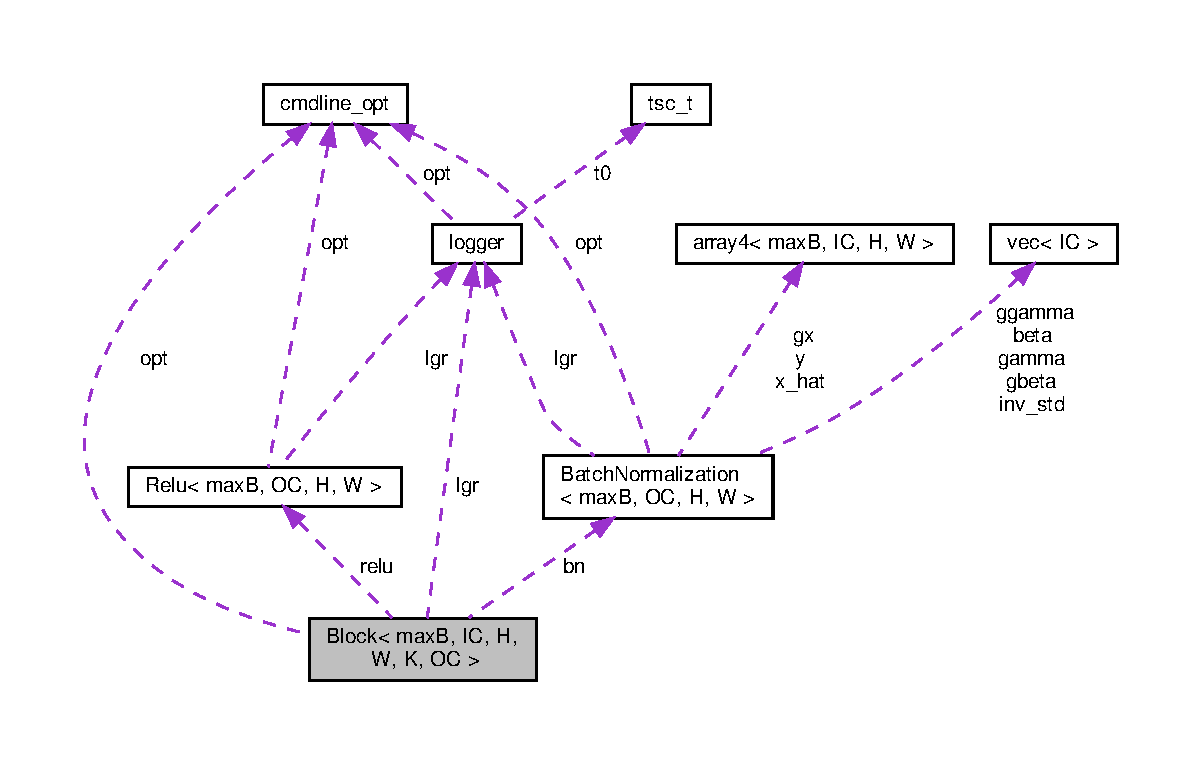
\includegraphics[width=350pt]{structBlock__coll__graph}
\end{center}
\end{figure}
\subsection*{Public Member Functions}
\begin{DoxyCompactItemize}
\item 
void \hyperlink{structBlock_a53eb5f86be4540cf491024b2b2783b42}{init} (\hyperlink{structcmdline__opt}{cmdline\+\_\+opt} \hyperlink{structBlock_ad91e112b767ccd7035a37873cbc121a9}{opt}, \hyperlink{structlogger}{logger} $\ast$\hyperlink{structBlock_a8e037036c2020d2ac98fc0792d3f84f4}{lgr}, \hyperlink{structrnd__gen__t}{rnd\+\_\+gen\+\_\+t} \&rg)
\begin{DoxyCompactList}\small\item\em initialize \end{DoxyCompactList}\item 
\hyperlink{structBlock}{Block}$<$ maxB, IC, H, W, K, OC $>$ $\ast$ \hyperlink{structBlock_a10734345f8456513bbd7c792b51656af}{copy} ()
\begin{DoxyCompactList}\small\item\em make a copy of this \end{DoxyCompactList}\item 
void \hyperlink{structBlock_a11093fd68976a6a40155cfb42397653c}{set\+\_\+dev} (\hyperlink{structBlock}{Block}$<$ maxB, IC, H, W, K, OC $>$ $\ast$\hyperlink{structBlock_a66767aae2045de05ce1dc09a92d164c4}{dev})
\begin{DoxyCompactList}\small\item\em set the device pointer for this and all subobjects \end{DoxyCompactList}\item 
void \hyperlink{structBlock_a971798b11f5cdc883880c0be2f143908}{make\+\_\+dev} ()
\begin{DoxyCompactList}\small\item\em if the algorithm is a gpu algorithm, allocate a device shadow of this object and set dev field of this and all subobjects. otherwise it sets all dev fields to null. \end{DoxyCompactList}\item 
void \hyperlink{structBlock_a46e9e4f4dcffddc409fa2b20263ea3b9}{del\+\_\+dev} ()
\begin{DoxyCompactList}\small\item\em if the algorithm is a gpu algorithm, dev field must not be null and deallocate it. \end{DoxyCompactList}\item 
\mbox{\Hypertarget{structBlock_a5dfc150c9bbf7eb57ab9488a5096df8d}\label{structBlock_a5dfc150c9bbf7eb57ab9488a5096df8d}} 
void \hyperlink{structBlock_a5dfc150c9bbf7eb57ab9488a5096df8d}{to\+\_\+dev} ()
\begin{DoxyCompactList}\small\item\em if the algorithm is a gpu algorithm, dev field must not be null and send the host data to the device memory \end{DoxyCompactList}\item 
\mbox{\Hypertarget{structBlock_aa0485907d27a19d4374e3ad09c5b9012}\label{structBlock_aa0485907d27a19d4374e3ad09c5b9012}} 
void \hyperlink{structBlock_aa0485907d27a19d4374e3ad09c5b9012}{to\+\_\+host} ()
\begin{DoxyCompactList}\small\item\em if the algorithm is a gpu algorithm, dev field must not be null and send the device data to the host memory \end{DoxyCompactList}\item 
void \hyperlink{structBlock_a3d431dfca3c47701c1c41e471ea17c8b}{update} (\hyperlink{vgg__util_8h_a1082d08aaa761215ec83e7149f27ad16}{real} eta)
\begin{DoxyCompactList}\small\item\em update weights of all sublayers with gradients that must have been computed \end{DoxyCompactList}\item 
\hyperlink{structarray4}{array4}$<$ maxB, OC, H, W $>$ \& \hyperlink{structBlock_a6a6ee3389b0ea5618109c9ca525ba9bf}{forward} (\hyperlink{structarray4}{array4}$<$ maxB, IC, H, W $>$ \&x)
\begin{DoxyCompactList}\small\item\em calc the loss function of a mini-\/batch (x) \end{DoxyCompactList}\item 
\hyperlink{structarray4}{array4}$<$ maxB, IC, H, W $>$ \& \hyperlink{structBlock_a86b4cafe64fbb5d045b7f2bc401d9ddc}{backward} (\hyperlink{structarray4}{array4}$<$ maxB, OC, H, W $>$ \&gy)
\begin{DoxyCompactList}\small\item\em calc the gradient of loss wrt the input (x) \end{DoxyCompactList}\item 
void \hyperlink{structBlock_a3752b971026c8a6506b34aef3c7e780b}{rand\+\_\+grad} (\hyperlink{structrnd__gen__t}{rnd\+\_\+gen\+\_\+t} \&rg, \hyperlink{vgg__util_8h_a1082d08aaa761215ec83e7149f27ad16}{real} p, \hyperlink{vgg__util_8h_a1082d08aaa761215ec83e7149f27ad16}{real} q)
\begin{DoxyCompactList}\small\item\em randomly set all gradients to values between p and q \end{DoxyCompactList}\item 
void \hyperlink{structBlock_ae0db7335928b4b004b644f2ef3ac1bc0}{set\+\_\+grad} (\hyperlink{structBlock}{Block}$<$ maxB, IC, H, W, K, OC $>$ \&o)
\begin{DoxyCompactList}\small\item\em set all gradients to gradients of another object \end{DoxyCompactList}\item 
\hyperlink{vgg__util_8h_a1082d08aaa761215ec83e7149f27ad16}{real} \hyperlink{structBlock_a69a63d3357f60c7b097e97169b175445}{gw\+\_\+dot\+\_\+gw} (\hyperlink{structBlock}{Block}$<$ maxB, IC, H, W, K, OC $>$ \&b)
\begin{DoxyCompactList}\small\item\em take the inner product of gradients \end{DoxyCompactList}\end{DoxyCompactItemize}
\subsection*{Public Attributes}
\begin{DoxyCompactItemize}
\item 
\hyperlink{structBlock}{Block}$<$ maxB, IC, H, W, K, OC $>$ $\ast$ \hyperlink{structBlock_a66767aae2045de05ce1dc09a92d164c4}{dev}
\item 
\hyperlink{structcmdline__opt}{cmdline\+\_\+opt} \hyperlink{structBlock_ad91e112b767ccd7035a37873cbc121a9}{opt}
\item 
\hyperlink{structlogger}{logger} $\ast$ \hyperlink{structBlock_a8e037036c2020d2ac98fc0792d3f84f4}{lgr}
\item 
\hyperlink{structConvolution2D}{Convolution2D}$<$ maxB, IC, H, W, K, OC $>$ \hyperlink{structBlock_aac195c086bc1302e8324aa1d89067668}{conv}
\item 
\hyperlink{structBatchNormalization}{Batch\+Normalization}$<$ maxB, OC, H, W $>$ \hyperlink{structBlock_afedad10fac693a934c1d72e24d478b6b}{bn}
\item 
\hyperlink{structRelu}{Relu}$<$ maxB, OC, H, W $>$ \hyperlink{structBlock_a019bcbd200d92669079eaa3c0c00ddfc}{relu}
\end{DoxyCompactItemize}


\subsection{Detailed Description}
\subsubsection*{template$<$idx\+\_\+t maxB, idx\+\_\+t IC, idx\+\_\+t H, idx\+\_\+t W, idx\+\_\+t K, idx\+\_\+t OC$>$\newline
struct Block$<$ max\+B, I\+C, H, W, K, O\+C $>$}

a block of three layers (convolution; batch normalization; relu) 


\begin{DoxyParams}{Parameters}
{\em (max\+B)} & the maximum number of images (batch size) \\
\hline
{\em (\+I\+C)} & the number of channels per input image (the original input has typically three channels for R\+GB. in hidden layers, it starts from 64 and goes up to 512 in the last hidden layer) \\
\hline
{\em (\+H)} & height of an image (32 for an input image, down to 1 in the last hidden layer) \\
\hline
{\em (\+W)} & width of an image (32 for an input image, down to 1 in the last hidden layer) \\
\hline
{\em (\+K)} & convolution kernel size (1). filter array has (2\+K+1)$\ast$(2\+K+1) elems) \\
\hline
{\em (\+O\+C)} & the number of channels per an output image\\
\hline
\end{DoxyParams}
this layer applies convolution, batch normalization and relu in this order. 

\subsection{Member Function Documentation}
\mbox{\Hypertarget{structBlock_a86b4cafe64fbb5d045b7f2bc401d9ddc}\label{structBlock_a86b4cafe64fbb5d045b7f2bc401d9ddc}} 
\index{Block@{Block}!backward@{backward}}
\index{backward@{backward}!Block@{Block}}
\subsubsection{\texorpdfstring{backward()}{backward()}}
{\footnotesize\ttfamily template$<$idx\+\_\+t maxB, idx\+\_\+t IC, idx\+\_\+t H, idx\+\_\+t W, idx\+\_\+t K, idx\+\_\+t OC$>$ \\
\hyperlink{structarray4}{array4}$<$maxB,IC,H,W$>$\& \hyperlink{structBlock}{Block}$<$ maxB, IC, H, W, K, OC $>$\+::backward (\begin{DoxyParamCaption}\item[{\hyperlink{structarray4}{array4}$<$ maxB, OC, H, W $>$ \&}]{gy }\end{DoxyParamCaption})\hspace{0.3cm}{\ttfamily [inline]}}



calc the gradient of loss wrt the input (x) 


\begin{DoxyParams}{Parameters}
{\em (gy)} & gradient of loss with respect to the output\\
\hline
\end{DoxyParams}
calc the gradient of loss wrt the input. along the way, it also calculates the gradient of loss wrt weights for all sublayers that have weights. since this is the entire network, gy is actually a vector whose components are all 1. (loss = sum of losses of each data). \begin{DoxySeeAlso}{See also}
\hyperlink{structBlock_a6a6ee3389b0ea5618109c9ca525ba9bf}{forward} 

\hyperlink{structBlock_a3d431dfca3c47701c1c41e471ea17c8b}{update} 
\end{DoxySeeAlso}
\mbox{\Hypertarget{structBlock_a10734345f8456513bbd7c792b51656af}\label{structBlock_a10734345f8456513bbd7c792b51656af}} 
\index{Block@{Block}!copy@{copy}}
\index{copy@{copy}!Block@{Block}}
\subsubsection{\texorpdfstring{copy()}{copy()}}
{\footnotesize\ttfamily template$<$idx\+\_\+t maxB, idx\+\_\+t IC, idx\+\_\+t H, idx\+\_\+t W, idx\+\_\+t K, idx\+\_\+t OC$>$ \\
\hyperlink{structBlock}{Block}$<$maxB,IC,H,W,K,OC$>$$\ast$ \hyperlink{structBlock}{Block}$<$ maxB, IC, H, W, K, OC $>$\+::copy (\begin{DoxyParamCaption}{ }\end{DoxyParamCaption})\hspace{0.3cm}{\ttfamily [inline]}}



make a copy of this 

if this object has a device pointer, the copy will have a device pointer too, but its contents are N\+OT copied \mbox{\Hypertarget{structBlock_a46e9e4f4dcffddc409fa2b20263ea3b9}\label{structBlock_a46e9e4f4dcffddc409fa2b20263ea3b9}} 
\index{Block@{Block}!del\+\_\+dev@{del\+\_\+dev}}
\index{del\+\_\+dev@{del\+\_\+dev}!Block@{Block}}
\subsubsection{\texorpdfstring{del\+\_\+dev()}{del\_dev()}}
{\footnotesize\ttfamily template$<$idx\+\_\+t maxB, idx\+\_\+t IC, idx\+\_\+t H, idx\+\_\+t W, idx\+\_\+t K, idx\+\_\+t OC$>$ \\
void \hyperlink{structBlock}{Block}$<$ maxB, IC, H, W, K, OC $>$\+::del\+\_\+dev (\begin{DoxyParamCaption}{ }\end{DoxyParamCaption})\hspace{0.3cm}{\ttfamily [inline]}}



if the algorithm is a gpu algorithm, dev field must not be null and deallocate it. 

\begin{DoxySeeAlso}{See also}
\hyperlink{structBlock_a971798b11f5cdc883880c0be2f143908}{make\+\_\+dev} 

\hyperlink{structBlock_a11093fd68976a6a40155cfb42397653c}{set\+\_\+dev} 
\end{DoxySeeAlso}
\mbox{\Hypertarget{structBlock_a6a6ee3389b0ea5618109c9ca525ba9bf}\label{structBlock_a6a6ee3389b0ea5618109c9ca525ba9bf}} 
\index{Block@{Block}!forward@{forward}}
\index{forward@{forward}!Block@{Block}}
\subsubsection{\texorpdfstring{forward()}{forward()}}
{\footnotesize\ttfamily template$<$idx\+\_\+t maxB, idx\+\_\+t IC, idx\+\_\+t H, idx\+\_\+t W, idx\+\_\+t K, idx\+\_\+t OC$>$ \\
\hyperlink{structarray4}{array4}$<$maxB,OC,H,W$>$\& \hyperlink{structBlock}{Block}$<$ maxB, IC, H, W, K, OC $>$\+::forward (\begin{DoxyParamCaption}\item[{\hyperlink{structarray4}{array4}$<$ maxB, IC, H, W $>$ \&}]{x }\end{DoxyParamCaption})\hspace{0.3cm}{\ttfamily [inline]}}



calc the loss function of a mini-\/batch (x) 


\begin{DoxyParams}{Parameters}
{\em (x)} & input images \\
\hline
\end{DoxyParams}
\begin{DoxySeeAlso}{See also}
\hyperlink{structBlock_a86b4cafe64fbb5d045b7f2bc401d9ddc}{backward} 

\hyperlink{structBlock_a3d431dfca3c47701c1c41e471ea17c8b}{update} 
\end{DoxySeeAlso}
\mbox{\Hypertarget{structBlock_a69a63d3357f60c7b097e97169b175445}\label{structBlock_a69a63d3357f60c7b097e97169b175445}} 
\index{Block@{Block}!gw\+\_\+dot\+\_\+gw@{gw\+\_\+dot\+\_\+gw}}
\index{gw\+\_\+dot\+\_\+gw@{gw\+\_\+dot\+\_\+gw}!Block@{Block}}
\subsubsection{\texorpdfstring{gw\+\_\+dot\+\_\+gw()}{gw\_dot\_gw()}}
{\footnotesize\ttfamily template$<$idx\+\_\+t maxB, idx\+\_\+t IC, idx\+\_\+t H, idx\+\_\+t W, idx\+\_\+t K, idx\+\_\+t OC$>$ \\
\hyperlink{vgg__util_8h_a1082d08aaa761215ec83e7149f27ad16}{real} \hyperlink{structBlock}{Block}$<$ maxB, IC, H, W, K, OC $>$\+::gw\+\_\+dot\+\_\+gw (\begin{DoxyParamCaption}\item[{\hyperlink{structBlock}{Block}$<$ maxB, IC, H, W, K, OC $>$ \&}]{b }\end{DoxyParamCaption})\hspace{0.3cm}{\ttfamily [inline]}}



take the inner product of gradients 


\begin{DoxyParams}{Parameters}
{\em (b)} & the object to take the inner product with\\
\hline
\end{DoxyParams}
take the inner product of this object\textquotesingle{}s gradients and b\textquotesingle{}s gradients \mbox{\Hypertarget{structBlock_a53eb5f86be4540cf491024b2b2783b42}\label{structBlock_a53eb5f86be4540cf491024b2b2783b42}} 
\index{Block@{Block}!init@{init}}
\index{init@{init}!Block@{Block}}
\subsubsection{\texorpdfstring{init()}{init()}}
{\footnotesize\ttfamily template$<$idx\+\_\+t maxB, idx\+\_\+t IC, idx\+\_\+t H, idx\+\_\+t W, idx\+\_\+t K, idx\+\_\+t OC$>$ \\
void \hyperlink{structBlock}{Block}$<$ maxB, IC, H, W, K, OC $>$\+::init (\begin{DoxyParamCaption}\item[{\hyperlink{structcmdline__opt}{cmdline\+\_\+opt}}]{opt,  }\item[{\hyperlink{structlogger}{logger} $\ast$}]{lgr,  }\item[{\hyperlink{structrnd__gen__t}{rnd\+\_\+gen\+\_\+t} \&}]{rg }\end{DoxyParamCaption})\hspace{0.3cm}{\ttfamily [inline]}}



initialize 


\begin{DoxyParams}{Parameters}
{\em (opt)} & command line options \\
\hline
{\em (lgr)} & logger \\
\hline
{\em (rg)} & random number generator for initializing weights \\
\hline
\end{DoxyParams}
\mbox{\Hypertarget{structBlock_a971798b11f5cdc883880c0be2f143908}\label{structBlock_a971798b11f5cdc883880c0be2f143908}} 
\index{Block@{Block}!make\+\_\+dev@{make\+\_\+dev}}
\index{make\+\_\+dev@{make\+\_\+dev}!Block@{Block}}
\subsubsection{\texorpdfstring{make\+\_\+dev()}{make\_dev()}}
{\footnotesize\ttfamily template$<$idx\+\_\+t maxB, idx\+\_\+t IC, idx\+\_\+t H, idx\+\_\+t W, idx\+\_\+t K, idx\+\_\+t OC$>$ \\
void \hyperlink{structBlock}{Block}$<$ maxB, IC, H, W, K, OC $>$\+::make\+\_\+dev (\begin{DoxyParamCaption}{ }\end{DoxyParamCaption})\hspace{0.3cm}{\ttfamily [inline]}}



if the algorithm is a gpu algorithm, allocate a device shadow of this object and set dev field of this and all subobjects. otherwise it sets all dev fields to null. 

\begin{DoxySeeAlso}{See also}
\hyperlink{structBlock_a11093fd68976a6a40155cfb42397653c}{set\+\_\+dev} 

\hyperlink{structBlock_a46e9e4f4dcffddc409fa2b20263ea3b9}{del\+\_\+dev} 
\end{DoxySeeAlso}
\mbox{\Hypertarget{structBlock_a3752b971026c8a6506b34aef3c7e780b}\label{structBlock_a3752b971026c8a6506b34aef3c7e780b}} 
\index{Block@{Block}!rand\+\_\+grad@{rand\+\_\+grad}}
\index{rand\+\_\+grad@{rand\+\_\+grad}!Block@{Block}}
\subsubsection{\texorpdfstring{rand\+\_\+grad()}{rand\_grad()}}
{\footnotesize\ttfamily template$<$idx\+\_\+t maxB, idx\+\_\+t IC, idx\+\_\+t H, idx\+\_\+t W, idx\+\_\+t K, idx\+\_\+t OC$>$ \\
void \hyperlink{structBlock}{Block}$<$ maxB, IC, H, W, K, OC $>$\+::rand\+\_\+grad (\begin{DoxyParamCaption}\item[{\hyperlink{structrnd__gen__t}{rnd\+\_\+gen\+\_\+t} \&}]{rg,  }\item[{\hyperlink{vgg__util_8h_a1082d08aaa761215ec83e7149f27ad16}{real}}]{p,  }\item[{\hyperlink{vgg__util_8h_a1082d08aaa761215ec83e7149f27ad16}{real}}]{q }\end{DoxyParamCaption})\hspace{0.3cm}{\ttfamily [inline]}}



randomly set all gradients to values between p and q 


\begin{DoxyParams}{Parameters}
{\em (rg)} & random number generator \\
\hline
{\em (p)} & minimum value of a component \\
\hline
{\em (q)} & maximum value of a component \\
\hline
\end{DoxyParams}
\mbox{\Hypertarget{structBlock_a11093fd68976a6a40155cfb42397653c}\label{structBlock_a11093fd68976a6a40155cfb42397653c}} 
\index{Block@{Block}!set\+\_\+dev@{set\+\_\+dev}}
\index{set\+\_\+dev@{set\+\_\+dev}!Block@{Block}}
\subsubsection{\texorpdfstring{set\+\_\+dev()}{set\_dev()}}
{\footnotesize\ttfamily template$<$idx\+\_\+t maxB, idx\+\_\+t IC, idx\+\_\+t H, idx\+\_\+t W, idx\+\_\+t K, idx\+\_\+t OC$>$ \\
void \hyperlink{structBlock}{Block}$<$ maxB, IC, H, W, K, OC $>$\+::set\+\_\+dev (\begin{DoxyParamCaption}\item[{\hyperlink{structBlock}{Block}$<$ maxB, IC, H, W, K, OC $>$ $\ast$}]{dev }\end{DoxyParamCaption})\hspace{0.3cm}{\ttfamily [inline]}}



set the device pointer for this and all subobjects 


\begin{DoxyParams}{Parameters}
{\em (dev)} & a device memory or null \\
\hline
\end{DoxyParams}
\begin{DoxySeeAlso}{See also}
\hyperlink{structBlock_a971798b11f5cdc883880c0be2f143908}{make\+\_\+dev} 

\hyperlink{structBlock_a46e9e4f4dcffddc409fa2b20263ea3b9}{del\+\_\+dev}
\end{DoxySeeAlso}
if dev is not null, dev fields of all subojects point to the corresponding subjects in the device memory. if dev is not null, all dev fields become null. \mbox{\Hypertarget{structBlock_ae0db7335928b4b004b644f2ef3ac1bc0}\label{structBlock_ae0db7335928b4b004b644f2ef3ac1bc0}} 
\index{Block@{Block}!set\+\_\+grad@{set\+\_\+grad}}
\index{set\+\_\+grad@{set\+\_\+grad}!Block@{Block}}
\subsubsection{\texorpdfstring{set\+\_\+grad()}{set\_grad()}}
{\footnotesize\ttfamily template$<$idx\+\_\+t maxB, idx\+\_\+t IC, idx\+\_\+t H, idx\+\_\+t W, idx\+\_\+t K, idx\+\_\+t OC$>$ \\
void \hyperlink{structBlock}{Block}$<$ maxB, IC, H, W, K, OC $>$\+::set\+\_\+grad (\begin{DoxyParamCaption}\item[{\hyperlink{structBlock}{Block}$<$ maxB, IC, H, W, K, OC $>$ \&}]{o }\end{DoxyParamCaption})\hspace{0.3cm}{\ttfamily [inline]}}



set all gradients to gradients of another object 


\begin{DoxyParams}{Parameters}
{\em (o)} & the object from which gradients get copied\\
\hline
\end{DoxyParams}
transfer gradients of o to this object \mbox{\Hypertarget{structBlock_a3d431dfca3c47701c1c41e471ea17c8b}\label{structBlock_a3d431dfca3c47701c1c41e471ea17c8b}} 
\index{Block@{Block}!update@{update}}
\index{update@{update}!Block@{Block}}
\subsubsection{\texorpdfstring{update()}{update()}}
{\footnotesize\ttfamily template$<$idx\+\_\+t maxB, idx\+\_\+t IC, idx\+\_\+t H, idx\+\_\+t W, idx\+\_\+t K, idx\+\_\+t OC$>$ \\
void \hyperlink{structBlock}{Block}$<$ maxB, IC, H, W, K, OC $>$\+::update (\begin{DoxyParamCaption}\item[{\hyperlink{vgg__util_8h_a1082d08aaa761215ec83e7149f27ad16}{real}}]{eta }\end{DoxyParamCaption})\hspace{0.3cm}{\ttfamily [inline]}}



update weights of all sublayers with gradients that must have been computed 


\begin{DoxyParams}{Parameters}
{\em (eta)} & the learning rate \\
\hline
\end{DoxyParams}
\begin{DoxySeeAlso}{See also}
\hyperlink{structBlock_a6a6ee3389b0ea5618109c9ca525ba9bf}{forward} 

\hyperlink{structBlock_a86b4cafe64fbb5d045b7f2bc401d9ddc}{backward} 
\end{DoxySeeAlso}


\subsection{Member Data Documentation}
\mbox{\Hypertarget{structBlock_afedad10fac693a934c1d72e24d478b6b}\label{structBlock_afedad10fac693a934c1d72e24d478b6b}} 
\index{Block@{Block}!bn@{bn}}
\index{bn@{bn}!Block@{Block}}
\subsubsection{\texorpdfstring{bn}{bn}}
{\footnotesize\ttfamily template$<$idx\+\_\+t maxB, idx\+\_\+t IC, idx\+\_\+t H, idx\+\_\+t W, idx\+\_\+t K, idx\+\_\+t OC$>$ \\
\hyperlink{structBatchNormalization}{Batch\+Normalization}$<$maxB,OC,H,W$>$ \hyperlink{structBlock}{Block}$<$ maxB, IC, H, W, K, OC $>$\+::bn}

batch normalization layer \mbox{\Hypertarget{structBlock_aac195c086bc1302e8324aa1d89067668}\label{structBlock_aac195c086bc1302e8324aa1d89067668}} 
\index{Block@{Block}!conv@{conv}}
\index{conv@{conv}!Block@{Block}}
\subsubsection{\texorpdfstring{conv}{conv}}
{\footnotesize\ttfamily template$<$idx\+\_\+t maxB, idx\+\_\+t IC, idx\+\_\+t H, idx\+\_\+t W, idx\+\_\+t K, idx\+\_\+t OC$>$ \\
\hyperlink{structConvolution2D}{Convolution2D}$<$maxB,IC,H,W,K,OC$>$ \hyperlink{structBlock}{Block}$<$ maxB, IC, H, W, K, OC $>$\+::conv}

convolution layer \mbox{\Hypertarget{structBlock_a66767aae2045de05ce1dc09a92d164c4}\label{structBlock_a66767aae2045de05ce1dc09a92d164c4}} 
\index{Block@{Block}!dev@{dev}}
\index{dev@{dev}!Block@{Block}}
\subsubsection{\texorpdfstring{dev}{dev}}
{\footnotesize\ttfamily template$<$idx\+\_\+t maxB, idx\+\_\+t IC, idx\+\_\+t H, idx\+\_\+t W, idx\+\_\+t K, idx\+\_\+t OC$>$ \\
\hyperlink{structBlock}{Block}$<$maxB,IC,H,W,K,OC$>$$\ast$ \hyperlink{structBlock}{Block}$<$ maxB, IC, H, W, K, OC $>$\+::dev}

device shadow \mbox{\Hypertarget{structBlock_a8e037036c2020d2ac98fc0792d3f84f4}\label{structBlock_a8e037036c2020d2ac98fc0792d3f84f4}} 
\index{Block@{Block}!lgr@{lgr}}
\index{lgr@{lgr}!Block@{Block}}
\subsubsection{\texorpdfstring{lgr}{lgr}}
{\footnotesize\ttfamily template$<$idx\+\_\+t maxB, idx\+\_\+t IC, idx\+\_\+t H, idx\+\_\+t W, idx\+\_\+t K, idx\+\_\+t OC$>$ \\
\hyperlink{structlogger}{logger}$\ast$ \hyperlink{structBlock}{Block}$<$ maxB, IC, H, W, K, OC $>$\+::lgr}

logger \mbox{\Hypertarget{structBlock_ad91e112b767ccd7035a37873cbc121a9}\label{structBlock_ad91e112b767ccd7035a37873cbc121a9}} 
\index{Block@{Block}!opt@{opt}}
\index{opt@{opt}!Block@{Block}}
\subsubsection{\texorpdfstring{opt}{opt}}
{\footnotesize\ttfamily template$<$idx\+\_\+t maxB, idx\+\_\+t IC, idx\+\_\+t H, idx\+\_\+t W, idx\+\_\+t K, idx\+\_\+t OC$>$ \\
\hyperlink{structcmdline__opt}{cmdline\+\_\+opt} \hyperlink{structBlock}{Block}$<$ maxB, IC, H, W, K, OC $>$\+::opt}

command line option \mbox{\Hypertarget{structBlock_a019bcbd200d92669079eaa3c0c00ddfc}\label{structBlock_a019bcbd200d92669079eaa3c0c00ddfc}} 
\index{Block@{Block}!relu@{relu}}
\index{relu@{relu}!Block@{Block}}
\subsubsection{\texorpdfstring{relu}{relu}}
{\footnotesize\ttfamily template$<$idx\+\_\+t maxB, idx\+\_\+t IC, idx\+\_\+t H, idx\+\_\+t W, idx\+\_\+t K, idx\+\_\+t OC$>$ \\
\hyperlink{structRelu}{Relu}$<$maxB,OC,H,W$>$ \hyperlink{structBlock}{Block}$<$ maxB, IC, H, W, K, OC $>$\+::relu}

rectified linear layer 

The documentation for this struct was generated from the following file\+:\begin{DoxyCompactItemize}
\item 
/home/tau/public\+\_\+html/lecture/parallel\+\_\+distributed/2018/handson/tau/parallel-\/distributed-\/handson/20vgg/include/\hyperlink{block_8h}{block.\+h}\end{DoxyCompactItemize}

\hypertarget{structcifar10__data__item}{}\section{cifar10\+\_\+data\+\_\+item$<$ IC, H, W $>$ Struct Template Reference}
\label{structcifar10__data__item}\index{cifar10\+\_\+data\+\_\+item$<$ I\+C, H, W $>$@{cifar10\+\_\+data\+\_\+item$<$ I\+C, H, W $>$}}


an input + true label  




{\ttfamily \#include $<$cifar.\+h$>$}

\subsection*{Public Member Functions}
\begin{DoxyCompactItemize}
\item 
\mbox{\Hypertarget{structcifar10__data__item_af006ac37b8c4ec720da2bb32da85d48e}\label{structcifar10__data__item_af006ac37b8c4ec720da2bb32da85d48e}} 
\hyperlink{vgg__util_8h_a1082d08aaa761215ec83e7149f27ad16}{real} \& \hyperlink{structcifar10__data__item_af006ac37b8c4ec720da2bb32da85d48e}{operator()} (\hyperlink{vgg__util_8h_a8e93478a00e685bea5e6a3f617bf03a3}{idx\+\_\+t} ic, \hyperlink{vgg__util_8h_a8e93478a00e685bea5e6a3f617bf03a3}{idx\+\_\+t} i, \hyperlink{vgg__util_8h_a8e93478a00e685bea5e6a3f617bf03a3}{idx\+\_\+t} j)
\begin{DoxyCompactList}\small\item\em get the (ic,i,j) pixel of the image \end{DoxyCompactList}\end{DoxyCompactItemize}
\subsection*{Public Attributes}
\begin{DoxyCompactItemize}
\item 
int \hyperlink{structcifar10__data__item_a316b080a202c3a6d2dc9d9b573bece65}{index}
\item 
\hyperlink{vgg__util_8h_a1082d08aaa761215ec83e7149f27ad16}{real} \hyperlink{structcifar10__data__item_a8bf2e62adbe5c3005f79fe3fd72d4e71}{w} \mbox{[}IC\mbox{]}\mbox{[}H\mbox{]}\mbox{[}W\mbox{]}
\item 
char \hyperlink{structcifar10__data__item_a90ed5833af38c869823166ea01c58edc}{label}
\end{DoxyCompactItemize}


\subsection{Detailed Description}
\subsubsection*{template$<$idx\+\_\+t IC, idx\+\_\+t H, idx\+\_\+t W$>$\newline
struct cifar10\+\_\+data\+\_\+item$<$ I\+C, H, W $>$}

an input + true label 

\subsection{Member Data Documentation}
\mbox{\Hypertarget{structcifar10__data__item_a316b080a202c3a6d2dc9d9b573bece65}\label{structcifar10__data__item_a316b080a202c3a6d2dc9d9b573bece65}} 
\index{cifar10\+\_\+data\+\_\+item@{cifar10\+\_\+data\+\_\+item}!index@{index}}
\index{index@{index}!cifar10\+\_\+data\+\_\+item@{cifar10\+\_\+data\+\_\+item}}
\subsubsection{\texorpdfstring{index}{index}}
{\footnotesize\ttfamily template$<$idx\+\_\+t IC, idx\+\_\+t H, idx\+\_\+t W$>$ \\
int \hyperlink{structcifar10__data__item}{cifar10\+\_\+data\+\_\+item}$<$ IC, H, W $>$\+::index}

index in the original file \mbox{\Hypertarget{structcifar10__data__item_a90ed5833af38c869823166ea01c58edc}\label{structcifar10__data__item_a90ed5833af38c869823166ea01c58edc}} 
\index{cifar10\+\_\+data\+\_\+item@{cifar10\+\_\+data\+\_\+item}!label@{label}}
\index{label@{label}!cifar10\+\_\+data\+\_\+item@{cifar10\+\_\+data\+\_\+item}}
\subsubsection{\texorpdfstring{label}{label}}
{\footnotesize\ttfamily template$<$idx\+\_\+t IC, idx\+\_\+t H, idx\+\_\+t W$>$ \\
char \hyperlink{structcifar10__data__item}{cifar10\+\_\+data\+\_\+item}$<$ IC, H, W $>$\+::label}

true label (0..9) \mbox{\Hypertarget{structcifar10__data__item_a8bf2e62adbe5c3005f79fe3fd72d4e71}\label{structcifar10__data__item_a8bf2e62adbe5c3005f79fe3fd72d4e71}} 
\index{cifar10\+\_\+data\+\_\+item@{cifar10\+\_\+data\+\_\+item}!w@{w}}
\index{w@{w}!cifar10\+\_\+data\+\_\+item@{cifar10\+\_\+data\+\_\+item}}
\subsubsection{\texorpdfstring{w}{w}}
{\footnotesize\ttfamily template$<$idx\+\_\+t IC, idx\+\_\+t H, idx\+\_\+t W$>$ \\
\hyperlink{vgg__util_8h_a1082d08aaa761215ec83e7149f27ad16}{real} \hyperlink{structcifar10__data__item}{cifar10\+\_\+data\+\_\+item}$<$ IC, H, W $>$\+::w\mbox{[}IC\mbox{]}\mbox{[}H\mbox{]}\mbox{[}W\mbox{]}}

pixels of an image 

The documentation for this struct was generated from the following file\+:\begin{DoxyCompactItemize}
\item 
/home/tau/public\+\_\+html/lecture/parallel\+\_\+distributed/2018/handson/tau/parallel-\/distributed-\/handson/20vgg/include/\hyperlink{cifar_8h}{cifar.\+h}\end{DoxyCompactItemize}

\hypertarget{structcifar10__dataset}{}\section{cifar10\+\_\+dataset$<$ maxB, IC, H, W $>$ Struct Template Reference}
\label{structcifar10__dataset}\index{cifar10\+\_\+dataset$<$ max\+B, I\+C, H, W $>$@{cifar10\+\_\+dataset$<$ max\+B, I\+C, H, W $>$}}


an entire cifar10 data  




{\ttfamily \#include $<$cifar.\+h$>$}



Collaboration diagram for cifar10\+\_\+dataset$<$ maxB, IC, H, W $>$\+:\nopagebreak
\begin{figure}[H]
\begin{center}
\leavevmode
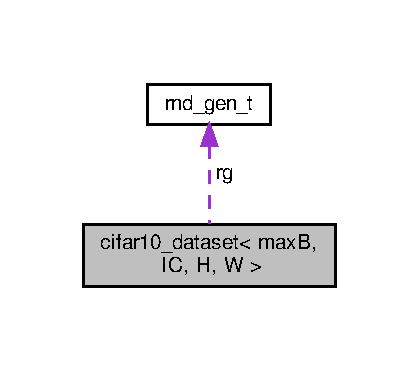
\includegraphics[width=201pt]{structcifar10__dataset__coll__graph}
\end{center}
\end{figure}
\subsection*{Public Member Functions}
\begin{DoxyCompactItemize}
\item 
void \hyperlink{structcifar10__dataset_a90bb8f4e440939589db017dbc89004c4}{set\+\_\+seed} (long sd)
\begin{DoxyCompactList}\small\item\em set seed for random number generator \end{DoxyCompactList}\item 
long \hyperlink{structcifar10__dataset_ad0025b0632ecfa9810d8a7c99d279f51}{get\+\_\+n\+\_\+data\+\_\+in\+\_\+file} (const char $\ast$cifar\+\_\+bin)
\begin{DoxyCompactList}\small\item\em count the number of images in a file (should be 10000) \end{DoxyCompactList}\item 
int \hyperlink{structcifar10__dataset_a4574eb110a71faac0e38445fd7be6fd2}{load} (\hyperlink{structlogger}{logger} \&lgr, const char $\ast$cifar\+\_\+bin, long n\+\_\+samples, long sample\+\_\+seed, double validate\+\_\+ratio)
\begin{DoxyCompactList}\small\item\em load training/validation data from the file \end{DoxyCompactList}\item 
void \hyperlink{structcifar10__dataset_acaa1adc9988bbb59550f778b82026ff8}{log\+\_\+dataset} (\hyperlink{structlogger}{logger} \&lgr)
\begin{DoxyCompactList}\small\item\em log dataset \end{DoxyCompactList}\item 
int \hyperlink{structcifar10__dataset_afafc5833390f1f3f9c2fefea15d643ca}{get\+\_\+data\+\_\+train} (\hyperlink{structarray4}{array4}$<$ maxB, IC, H, W $>$ \&x, \hyperlink{structivec}{ivec}$<$ maxB $>$ \&t, \hyperlink{vgg__util_8h_a8e93478a00e685bea5e6a3f617bf03a3}{idx\+\_\+t} B)
\begin{DoxyCompactList}\small\item\em load x and t with the a mini batch of B images \end{DoxyCompactList}\item 
int \hyperlink{structcifar10__dataset_a4176a67684d105dac1c95a1556761173}{get\+\_\+data\+\_\+validate} (\hyperlink{structarray4}{array4}$<$ maxB, IC, H, W $>$ \&x, \hyperlink{structivec}{ivec}$<$ maxB $>$ \&t, \hyperlink{vgg__util_8h_a8e93478a00e685bea5e6a3f617bf03a3}{idx\+\_\+t} from, \hyperlink{vgg__util_8h_a8e93478a00e685bea5e6a3f617bf03a3}{idx\+\_\+t} to)
\begin{DoxyCompactList}\small\item\em load x and t with a part of validation data (from\+:to) \end{DoxyCompactList}\end{DoxyCompactItemize}
\subsection*{Public Attributes}
\begin{DoxyCompactItemize}
\item 
long \hyperlink{structcifar10__dataset_a60c9f64838a155a1127912cf190b3ed0}{n\+\_\+data}
\item 
long \hyperlink{structcifar10__dataset_a0f447993bfd499e4222e66dca3e111a0}{n\+\_\+validate}
\item 
long \hyperlink{structcifar10__dataset_ac6e5dbe7c30b683d01e600901c51e010}{n\+\_\+train}
\item 
\hyperlink{structcifar10__data__item}{cifar10\+\_\+data\+\_\+item}$<$ IC, H, W $>$ $\ast$ \hyperlink{structcifar10__dataset_a8c4071c746bf18e875b9e7975c7929fd}{dataset}
\item 
\hyperlink{structcifar10__data__item}{cifar10\+\_\+data\+\_\+item}$<$ IC, H, W $>$ $\ast$ \hyperlink{structcifar10__dataset_a3264803c2eb493dabaedb7eca4d7725f}{validate}
\item 
\hyperlink{structcifar10__data__item}{cifar10\+\_\+data\+\_\+item}$<$ IC, H, W $>$ $\ast$ \hyperlink{structcifar10__dataset_a0c64c36b940f91c63a9d5f89360f5335}{train}
\item 
\hyperlink{structrnd__gen__t}{rnd\+\_\+gen\+\_\+t} \hyperlink{structcifar10__dataset_a59998ba824d0a527fe0f6e7aad0693eb}{rg}
\end{DoxyCompactItemize}


\subsection{Detailed Description}
\subsubsection*{template$<$idx\+\_\+t maxB, idx\+\_\+t IC, idx\+\_\+t H, idx\+\_\+t W$>$\newline
struct cifar10\+\_\+dataset$<$ max\+B, I\+C, H, W $>$}

an entire cifar10 data 

\subsection{Member Function Documentation}
\mbox{\Hypertarget{structcifar10__dataset_afafc5833390f1f3f9c2fefea15d643ca}\label{structcifar10__dataset_afafc5833390f1f3f9c2fefea15d643ca}} 
\index{cifar10\+\_\+dataset@{cifar10\+\_\+dataset}!get\+\_\+data\+\_\+train@{get\+\_\+data\+\_\+train}}
\index{get\+\_\+data\+\_\+train@{get\+\_\+data\+\_\+train}!cifar10\+\_\+dataset@{cifar10\+\_\+dataset}}
\subsubsection{\texorpdfstring{get\+\_\+data\+\_\+train()}{get\_data\_train()}}
{\footnotesize\ttfamily template$<$idx\+\_\+t maxB, idx\+\_\+t IC, idx\+\_\+t H, idx\+\_\+t W$>$ \\
int \hyperlink{structcifar10__dataset}{cifar10\+\_\+dataset}$<$ maxB, IC, H, W $>$\+::get\+\_\+data\+\_\+train (\begin{DoxyParamCaption}\item[{\hyperlink{structarray4}{array4}$<$ maxB, IC, H, W $>$ \&}]{x,  }\item[{\hyperlink{structivec}{ivec}$<$ maxB $>$ \&}]{t,  }\item[{\hyperlink{vgg__util_8h_a8e93478a00e685bea5e6a3f617bf03a3}{idx\+\_\+t}}]{B }\end{DoxyParamCaption})\hspace{0.3cm}{\ttfamily [inline]}}



load x and t with the a mini batch of B images 


\begin{DoxyParams}{Parameters}
{\em (x)} & array to load images into \\
\hline
{\em (t)} & array to load true labels into \\
\hline
{\em (\+B)} & the number of images to pick \\
\hline
\end{DoxyParams}
\mbox{\Hypertarget{structcifar10__dataset_a4176a67684d105dac1c95a1556761173}\label{structcifar10__dataset_a4176a67684d105dac1c95a1556761173}} 
\index{cifar10\+\_\+dataset@{cifar10\+\_\+dataset}!get\+\_\+data\+\_\+validate@{get\+\_\+data\+\_\+validate}}
\index{get\+\_\+data\+\_\+validate@{get\+\_\+data\+\_\+validate}!cifar10\+\_\+dataset@{cifar10\+\_\+dataset}}
\subsubsection{\texorpdfstring{get\+\_\+data\+\_\+validate()}{get\_data\_validate()}}
{\footnotesize\ttfamily template$<$idx\+\_\+t maxB, idx\+\_\+t IC, idx\+\_\+t H, idx\+\_\+t W$>$ \\
int \hyperlink{structcifar10__dataset}{cifar10\+\_\+dataset}$<$ maxB, IC, H, W $>$\+::get\+\_\+data\+\_\+validate (\begin{DoxyParamCaption}\item[{\hyperlink{structarray4}{array4}$<$ maxB, IC, H, W $>$ \&}]{x,  }\item[{\hyperlink{structivec}{ivec}$<$ maxB $>$ \&}]{t,  }\item[{\hyperlink{vgg__util_8h_a8e93478a00e685bea5e6a3f617bf03a3}{idx\+\_\+t}}]{from,  }\item[{\hyperlink{vgg__util_8h_a8e93478a00e685bea5e6a3f617bf03a3}{idx\+\_\+t}}]{to }\end{DoxyParamCaption})\hspace{0.3cm}{\ttfamily [inline]}}



load x and t with a part of validation data (from\+:to) 


\begin{DoxyParams}{Parameters}
{\em (x)} & array to load images into \\
\hline
{\em (t)} & array to load true labels into \\
\hline
{\em (from)} & the first validation image to return \\
\hline
{\em (to)} & the last validation image to load + 1 \\
\hline
\end{DoxyParams}
\mbox{\Hypertarget{structcifar10__dataset_ad0025b0632ecfa9810d8a7c99d279f51}\label{structcifar10__dataset_ad0025b0632ecfa9810d8a7c99d279f51}} 
\index{cifar10\+\_\+dataset@{cifar10\+\_\+dataset}!get\+\_\+n\+\_\+data\+\_\+in\+\_\+file@{get\+\_\+n\+\_\+data\+\_\+in\+\_\+file}}
\index{get\+\_\+n\+\_\+data\+\_\+in\+\_\+file@{get\+\_\+n\+\_\+data\+\_\+in\+\_\+file}!cifar10\+\_\+dataset@{cifar10\+\_\+dataset}}
\subsubsection{\texorpdfstring{get\+\_\+n\+\_\+data\+\_\+in\+\_\+file()}{get\_n\_data\_in\_file()}}
{\footnotesize\ttfamily template$<$idx\+\_\+t maxB, idx\+\_\+t IC, idx\+\_\+t H, idx\+\_\+t W$>$ \\
long \hyperlink{structcifar10__dataset}{cifar10\+\_\+dataset}$<$ maxB, IC, H, W $>$\+::get\+\_\+n\+\_\+data\+\_\+in\+\_\+file (\begin{DoxyParamCaption}\item[{const char $\ast$}]{cifar\+\_\+bin }\end{DoxyParamCaption})\hspace{0.3cm}{\ttfamily [inline]}}



count the number of images in a file (should be 10000) 


\begin{DoxyParams}{Parameters}
{\em (cifar\+\_\+bin)} & the name of the file to read data from \\
\hline
\end{DoxyParams}
\mbox{\Hypertarget{structcifar10__dataset_a4574eb110a71faac0e38445fd7be6fd2}\label{structcifar10__dataset_a4574eb110a71faac0e38445fd7be6fd2}} 
\index{cifar10\+\_\+dataset@{cifar10\+\_\+dataset}!load@{load}}
\index{load@{load}!cifar10\+\_\+dataset@{cifar10\+\_\+dataset}}
\subsubsection{\texorpdfstring{load()}{load()}}
{\footnotesize\ttfamily template$<$idx\+\_\+t maxB, idx\+\_\+t IC, idx\+\_\+t H, idx\+\_\+t W$>$ \\
int \hyperlink{structcifar10__dataset}{cifar10\+\_\+dataset}$<$ maxB, IC, H, W $>$\+::load (\begin{DoxyParamCaption}\item[{\hyperlink{structlogger}{logger} \&}]{lgr,  }\item[{const char $\ast$}]{cifar\+\_\+bin,  }\item[{long}]{n\+\_\+samples,  }\item[{long}]{sample\+\_\+seed,  }\item[{double}]{validate\+\_\+ratio }\end{DoxyParamCaption})\hspace{0.3cm}{\ttfamily [inline]}}



load training/validation data from the file 


\begin{DoxyParams}{Parameters}
{\em (lgr)} & logger \\
\hline
{\em (cifar\+\_\+bin)} & the name of the file to read data from \\
\hline
{\em (n\+\_\+samples)} & the number of data used \\
\hline
{\em (sample\+\_\+seed)} & seed of the random number generator to pick training and validation data \\
\hline
{\em (validate\+\_\+ratio)} & leave this much for validation ($<$1.\+0) \\
\hline
\end{DoxyParams}
\mbox{\Hypertarget{structcifar10__dataset_acaa1adc9988bbb59550f778b82026ff8}\label{structcifar10__dataset_acaa1adc9988bbb59550f778b82026ff8}} 
\index{cifar10\+\_\+dataset@{cifar10\+\_\+dataset}!log\+\_\+dataset@{log\+\_\+dataset}}
\index{log\+\_\+dataset@{log\+\_\+dataset}!cifar10\+\_\+dataset@{cifar10\+\_\+dataset}}
\subsubsection{\texorpdfstring{log\+\_\+dataset()}{log\_dataset()}}
{\footnotesize\ttfamily template$<$idx\+\_\+t maxB, idx\+\_\+t IC, idx\+\_\+t H, idx\+\_\+t W$>$ \\
void \hyperlink{structcifar10__dataset}{cifar10\+\_\+dataset}$<$ maxB, IC, H, W $>$\+::log\+\_\+dataset (\begin{DoxyParamCaption}\item[{\hyperlink{structlogger}{logger} \&}]{lgr }\end{DoxyParamCaption})\hspace{0.3cm}{\ttfamily [inline]}}



log dataset 


\begin{DoxyParams}{Parameters}
{\em (lgr)} & logger \\
\hline
\end{DoxyParams}
\mbox{\Hypertarget{structcifar10__dataset_a90bb8f4e440939589db017dbc89004c4}\label{structcifar10__dataset_a90bb8f4e440939589db017dbc89004c4}} 
\index{cifar10\+\_\+dataset@{cifar10\+\_\+dataset}!set\+\_\+seed@{set\+\_\+seed}}
\index{set\+\_\+seed@{set\+\_\+seed}!cifar10\+\_\+dataset@{cifar10\+\_\+dataset}}
\subsubsection{\texorpdfstring{set\+\_\+seed()}{set\_seed()}}
{\footnotesize\ttfamily template$<$idx\+\_\+t maxB, idx\+\_\+t IC, idx\+\_\+t H, idx\+\_\+t W$>$ \\
void \hyperlink{structcifar10__dataset}{cifar10\+\_\+dataset}$<$ maxB, IC, H, W $>$\+::set\+\_\+seed (\begin{DoxyParamCaption}\item[{long}]{sd }\end{DoxyParamCaption})\hspace{0.3cm}{\ttfamily [inline]}}



set seed for random number generator 

\begin{DoxySeeAlso}{See also}
(sd) seed 
\end{DoxySeeAlso}


\subsection{Member Data Documentation}
\mbox{\Hypertarget{structcifar10__dataset_a8c4071c746bf18e875b9e7975c7929fd}\label{structcifar10__dataset_a8c4071c746bf18e875b9e7975c7929fd}} 
\index{cifar10\+\_\+dataset@{cifar10\+\_\+dataset}!dataset@{dataset}}
\index{dataset@{dataset}!cifar10\+\_\+dataset@{cifar10\+\_\+dataset}}
\subsubsection{\texorpdfstring{dataset}{dataset}}
{\footnotesize\ttfamily template$<$idx\+\_\+t maxB, idx\+\_\+t IC, idx\+\_\+t H, idx\+\_\+t W$>$ \\
\hyperlink{structcifar10__data__item}{cifar10\+\_\+data\+\_\+item}$<$IC,H,W$>$$\ast$ \hyperlink{structcifar10__dataset}{cifar10\+\_\+dataset}$<$ maxB, IC, H, W $>$\+::dataset}

whole dataset (n\+\_\+data items) \mbox{\Hypertarget{structcifar10__dataset_a60c9f64838a155a1127912cf190b3ed0}\label{structcifar10__dataset_a60c9f64838a155a1127912cf190b3ed0}} 
\index{cifar10\+\_\+dataset@{cifar10\+\_\+dataset}!n\+\_\+data@{n\+\_\+data}}
\index{n\+\_\+data@{n\+\_\+data}!cifar10\+\_\+dataset@{cifar10\+\_\+dataset}}
\subsubsection{\texorpdfstring{n\+\_\+data}{n\_data}}
{\footnotesize\ttfamily template$<$idx\+\_\+t maxB, idx\+\_\+t IC, idx\+\_\+t H, idx\+\_\+t W$>$ \\
long \hyperlink{structcifar10__dataset}{cifar10\+\_\+dataset}$<$ maxB, IC, H, W $>$\+::n\+\_\+data}

the total number of images \mbox{\Hypertarget{structcifar10__dataset_ac6e5dbe7c30b683d01e600901c51e010}\label{structcifar10__dataset_ac6e5dbe7c30b683d01e600901c51e010}} 
\index{cifar10\+\_\+dataset@{cifar10\+\_\+dataset}!n\+\_\+train@{n\+\_\+train}}
\index{n\+\_\+train@{n\+\_\+train}!cifar10\+\_\+dataset@{cifar10\+\_\+dataset}}
\subsubsection{\texorpdfstring{n\+\_\+train}{n\_train}}
{\footnotesize\ttfamily template$<$idx\+\_\+t maxB, idx\+\_\+t IC, idx\+\_\+t H, idx\+\_\+t W$>$ \\
long \hyperlink{structcifar10__dataset}{cifar10\+\_\+dataset}$<$ maxB, IC, H, W $>$\+::n\+\_\+train}

the number of traininig images \mbox{\Hypertarget{structcifar10__dataset_a0f447993bfd499e4222e66dca3e111a0}\label{structcifar10__dataset_a0f447993bfd499e4222e66dca3e111a0}} 
\index{cifar10\+\_\+dataset@{cifar10\+\_\+dataset}!n\+\_\+validate@{n\+\_\+validate}}
\index{n\+\_\+validate@{n\+\_\+validate}!cifar10\+\_\+dataset@{cifar10\+\_\+dataset}}
\subsubsection{\texorpdfstring{n\+\_\+validate}{n\_validate}}
{\footnotesize\ttfamily template$<$idx\+\_\+t maxB, idx\+\_\+t IC, idx\+\_\+t H, idx\+\_\+t W$>$ \\
long \hyperlink{structcifar10__dataset}{cifar10\+\_\+dataset}$<$ maxB, IC, H, W $>$\+::n\+\_\+validate}

the number of validation images \mbox{\Hypertarget{structcifar10__dataset_a59998ba824d0a527fe0f6e7aad0693eb}\label{structcifar10__dataset_a59998ba824d0a527fe0f6e7aad0693eb}} 
\index{cifar10\+\_\+dataset@{cifar10\+\_\+dataset}!rg@{rg}}
\index{rg@{rg}!cifar10\+\_\+dataset@{cifar10\+\_\+dataset}}
\subsubsection{\texorpdfstring{rg}{rg}}
{\footnotesize\ttfamily template$<$idx\+\_\+t maxB, idx\+\_\+t IC, idx\+\_\+t H, idx\+\_\+t W$>$ \\
\hyperlink{structrnd__gen__t}{rnd\+\_\+gen\+\_\+t} \hyperlink{structcifar10__dataset}{cifar10\+\_\+dataset}$<$ maxB, IC, H, W $>$\+::rg}

random number generator to pick images for a mini batch \mbox{\Hypertarget{structcifar10__dataset_a0c64c36b940f91c63a9d5f89360f5335}\label{structcifar10__dataset_a0c64c36b940f91c63a9d5f89360f5335}} 
\index{cifar10\+\_\+dataset@{cifar10\+\_\+dataset}!train@{train}}
\index{train@{train}!cifar10\+\_\+dataset@{cifar10\+\_\+dataset}}
\subsubsection{\texorpdfstring{train}{train}}
{\footnotesize\ttfamily template$<$idx\+\_\+t maxB, idx\+\_\+t IC, idx\+\_\+t H, idx\+\_\+t W$>$ \\
\hyperlink{structcifar10__data__item}{cifar10\+\_\+data\+\_\+item}$<$IC,H,W$>$$\ast$ \hyperlink{structcifar10__dataset}{cifar10\+\_\+dataset}$<$ maxB, IC, H, W $>$\+::train}

training part (remaining items) \mbox{\Hypertarget{structcifar10__dataset_a3264803c2eb493dabaedb7eca4d7725f}\label{structcifar10__dataset_a3264803c2eb493dabaedb7eca4d7725f}} 
\index{cifar10\+\_\+dataset@{cifar10\+\_\+dataset}!validate@{validate}}
\index{validate@{validate}!cifar10\+\_\+dataset@{cifar10\+\_\+dataset}}
\subsubsection{\texorpdfstring{validate}{validate}}
{\footnotesize\ttfamily template$<$idx\+\_\+t maxB, idx\+\_\+t IC, idx\+\_\+t H, idx\+\_\+t W$>$ \\
\hyperlink{structcifar10__data__item}{cifar10\+\_\+data\+\_\+item}$<$IC,H,W$>$$\ast$ \hyperlink{structcifar10__dataset}{cifar10\+\_\+dataset}$<$ maxB, IC, H, W $>$\+::validate}

validation part (first n\+\_\+validate items) 

The documentation for this struct was generated from the following file\+:\begin{DoxyCompactItemize}
\item 
/home/tau/public\+\_\+html/lecture/parallel\+\_\+distributed/2018/handson/tau/parallel-\/distributed-\/handson/20vgg/include/\hyperlink{cifar_8h}{cifar.\+h}\end{DoxyCompactItemize}

\hypertarget{structcmdline__opt}{}\section{cmdline\+\_\+opt Struct Reference}
\label{structcmdline__opt}\index{cmdline\+\_\+opt@{cmdline\+\_\+opt}}


command line options  




{\ttfamily \#include $<$vgg\+\_\+util.\+h$>$}

\subsection*{Public Member Functions}
\begin{DoxyCompactItemize}
\item 
\mbox{\Hypertarget{structcmdline__opt_a389b760269a58bc462e8b429e4ef914e}\label{structcmdline__opt_a389b760269a58bc462e8b429e4ef914e}} 
\hyperlink{structcmdline__opt_a389b760269a58bc462e8b429e4ef914e}{cmdline\+\_\+opt} ()
\begin{DoxyCompactList}\small\item\em initialize a command line object with default vaules \end{DoxyCompactList}\end{DoxyCompactItemize}
\subsection*{Public Attributes}
\begin{DoxyCompactItemize}
\item 
int \hyperlink{structcmdline__opt_a2212d80547e3ae3504942006440f7285}{verbose}
\item 
const char $\ast$ \hyperlink{structcmdline__opt_aeaf0e85613dea855a29a691b5915e81a}{cifar\+\_\+data}
\item 
\hyperlink{vgg__util_8h_a8e93478a00e685bea5e6a3f617bf03a3}{idx\+\_\+t} \hyperlink{structcmdline__opt_a417b11f5b6a5213e293ce930a471a786}{batch\+\_\+sz}
\item 
\hyperlink{vgg__util_8h_a1082d08aaa761215ec83e7149f27ad16}{real} \hyperlink{structcmdline__opt_a69793f204ee2703085e3153062f0a3fd}{learnrate}
\item 
long \hyperlink{structcmdline__opt_a430664c4a225528c56f959765371755d}{iters}
\item 
long \hyperlink{structcmdline__opt_a36b99fa5f7fa96a44170687afc327f07}{partial\+\_\+data}
\item 
int \hyperlink{structcmdline__opt_a2e2f53ec465901071633192bfdec032a}{single\+\_\+batch}
\item 
int \hyperlink{structcmdline__opt_a0db00c69f0bfa206b17748c0b9ca1d0b}{dropout}
\item 
double \hyperlink{structcmdline__opt_a559a5437432ab522d6f2749876147029}{validate\+\_\+ratio}
\item 
double \hyperlink{structcmdline__opt_a93fd0f470a52208842dd7257b83df50b}{validate\+\_\+interval}
\item 
long \hyperlink{structcmdline__opt_aa92b1cc0e53246cc03bbab7fbc84b5ae}{sample\+\_\+seed}
\item 
long \hyperlink{structcmdline__opt_a70133aad1b243d44e1be18be81633939}{weight\+\_\+seed}
\item 
long \hyperlink{structcmdline__opt_a8618cfd6b437743f58258b580d59b466}{dropout\+\_\+seed}
\item 
long \hyperlink{structcmdline__opt_a046deb2b2e8e313a27f753cf4aa9883c}{partial\+\_\+data\+\_\+seed}
\item 
int \hyperlink{structcmdline__opt_a5e70c87e86e82f9d42f6eb341f0902e3}{grad\+\_\+dbg}
\item 
const char $\ast$ \hyperlink{structcmdline__opt_aa5b05fde2a12fcab6f9ce0baf3e29d29}{algo\+\_\+s}
\item 
\hyperlink{vgg__util_8h_ae1267137aba8cc25a02220492efa7d3c}{algo\+\_\+t} \hyperlink{structcmdline__opt_a4506cc13417cfb1379411fb497ae3c39}{algo}
\item 
int \hyperlink{structcmdline__opt_acb8b225214983d009415a26f2e45eb65}{gpu\+\_\+algo}
\item 
const char $\ast$ \hyperlink{structcmdline__opt_a0ecd10b9b45fb70719fb85fff85469ad}{log}
\item 
int \hyperlink{structcmdline__opt_afcc6982691bd1f6dfac42dbf423f9ead}{help}
\item 
int \hyperlink{structcmdline__opt_a500dde11d2a0ee2e4dff8e4144083556}{error}
\end{DoxyCompactItemize}


\subsection{Detailed Description}
command line options 

\subsection{Member Data Documentation}
\mbox{\Hypertarget{structcmdline__opt_a4506cc13417cfb1379411fb497ae3c39}\label{structcmdline__opt_a4506cc13417cfb1379411fb497ae3c39}} 
\index{cmdline\+\_\+opt@{cmdline\+\_\+opt}!algo@{algo}}
\index{algo@{algo}!cmdline\+\_\+opt@{cmdline\+\_\+opt}}
\subsubsection{\texorpdfstring{algo}{algo}}
{\footnotesize\ttfamily \hyperlink{vgg__util_8h_ae1267137aba8cc25a02220492efa7d3c}{algo\+\_\+t} cmdline\+\_\+opt\+::algo}

parse\+\_\+algo(algo\+\_\+s) \mbox{\Hypertarget{structcmdline__opt_aa5b05fde2a12fcab6f9ce0baf3e29d29}\label{structcmdline__opt_aa5b05fde2a12fcab6f9ce0baf3e29d29}} 
\index{cmdline\+\_\+opt@{cmdline\+\_\+opt}!algo\+\_\+s@{algo\+\_\+s}}
\index{algo\+\_\+s@{algo\+\_\+s}!cmdline\+\_\+opt@{cmdline\+\_\+opt}}
\subsubsection{\texorpdfstring{algo\+\_\+s}{algo\_s}}
{\footnotesize\ttfamily const char$\ast$ cmdline\+\_\+opt\+::algo\+\_\+s}

string passed to --algo \mbox{\Hypertarget{structcmdline__opt_a417b11f5b6a5213e293ce930a471a786}\label{structcmdline__opt_a417b11f5b6a5213e293ce930a471a786}} 
\index{cmdline\+\_\+opt@{cmdline\+\_\+opt}!batch\+\_\+sz@{batch\+\_\+sz}}
\index{batch\+\_\+sz@{batch\+\_\+sz}!cmdline\+\_\+opt@{cmdline\+\_\+opt}}
\subsubsection{\texorpdfstring{batch\+\_\+sz}{batch\_sz}}
{\footnotesize\ttfamily \hyperlink{vgg__util_8h_a8e93478a00e685bea5e6a3f617bf03a3}{idx\+\_\+t} cmdline\+\_\+opt\+::batch\+\_\+sz}

batch size \mbox{\Hypertarget{structcmdline__opt_aeaf0e85613dea855a29a691b5915e81a}\label{structcmdline__opt_aeaf0e85613dea855a29a691b5915e81a}} 
\index{cmdline\+\_\+opt@{cmdline\+\_\+opt}!cifar\+\_\+data@{cifar\+\_\+data}}
\index{cifar\+\_\+data@{cifar\+\_\+data}!cmdline\+\_\+opt@{cmdline\+\_\+opt}}
\subsubsection{\texorpdfstring{cifar\+\_\+data}{cifar\_data}}
{\footnotesize\ttfamily const char$\ast$ cmdline\+\_\+opt\+::cifar\+\_\+data}

data file \mbox{\Hypertarget{structcmdline__opt_a0db00c69f0bfa206b17748c0b9ca1d0b}\label{structcmdline__opt_a0db00c69f0bfa206b17748c0b9ca1d0b}} 
\index{cmdline\+\_\+opt@{cmdline\+\_\+opt}!dropout@{dropout}}
\index{dropout@{dropout}!cmdline\+\_\+opt@{cmdline\+\_\+opt}}
\subsubsection{\texorpdfstring{dropout}{dropout}}
{\footnotesize\ttfamily int cmdline\+\_\+opt\+::dropout}

1 if we use dropout \mbox{\Hypertarget{structcmdline__opt_a8618cfd6b437743f58258b580d59b466}\label{structcmdline__opt_a8618cfd6b437743f58258b580d59b466}} 
\index{cmdline\+\_\+opt@{cmdline\+\_\+opt}!dropout\+\_\+seed@{dropout\+\_\+seed}}
\index{dropout\+\_\+seed@{dropout\+\_\+seed}!cmdline\+\_\+opt@{cmdline\+\_\+opt}}
\subsubsection{\texorpdfstring{dropout\+\_\+seed}{dropout\_seed}}
{\footnotesize\ttfamily long cmdline\+\_\+opt\+::dropout\+\_\+seed}

random seed to determine dropout \mbox{\Hypertarget{structcmdline__opt_a500dde11d2a0ee2e4dff8e4144083556}\label{structcmdline__opt_a500dde11d2a0ee2e4dff8e4144083556}} 
\index{cmdline\+\_\+opt@{cmdline\+\_\+opt}!error@{error}}
\index{error@{error}!cmdline\+\_\+opt@{cmdline\+\_\+opt}}
\subsubsection{\texorpdfstring{error}{error}}
{\footnotesize\ttfamily int cmdline\+\_\+opt\+::error}

set to one if any option is invalid \mbox{\Hypertarget{structcmdline__opt_acb8b225214983d009415a26f2e45eb65}\label{structcmdline__opt_acb8b225214983d009415a26f2e45eb65}} 
\index{cmdline\+\_\+opt@{cmdline\+\_\+opt}!gpu\+\_\+algo@{gpu\+\_\+algo}}
\index{gpu\+\_\+algo@{gpu\+\_\+algo}!cmdline\+\_\+opt@{cmdline\+\_\+opt}}
\subsubsection{\texorpdfstring{gpu\+\_\+algo}{gpu\_algo}}
{\footnotesize\ttfamily int cmdline\+\_\+opt\+::gpu\+\_\+algo}

1 if this is a G\+PU algorithm \mbox{\Hypertarget{structcmdline__opt_a5e70c87e86e82f9d42f6eb341f0902e3}\label{structcmdline__opt_a5e70c87e86e82f9d42f6eb341f0902e3}} 
\index{cmdline\+\_\+opt@{cmdline\+\_\+opt}!grad\+\_\+dbg@{grad\+\_\+dbg}}
\index{grad\+\_\+dbg@{grad\+\_\+dbg}!cmdline\+\_\+opt@{cmdline\+\_\+opt}}
\subsubsection{\texorpdfstring{grad\+\_\+dbg}{grad\_dbg}}
{\footnotesize\ttfamily int cmdline\+\_\+opt\+::grad\+\_\+dbg}

1 if we debug gradient \mbox{\Hypertarget{structcmdline__opt_afcc6982691bd1f6dfac42dbf423f9ead}\label{structcmdline__opt_afcc6982691bd1f6dfac42dbf423f9ead}} 
\index{cmdline\+\_\+opt@{cmdline\+\_\+opt}!help@{help}}
\index{help@{help}!cmdline\+\_\+opt@{cmdline\+\_\+opt}}
\subsubsection{\texorpdfstring{help}{help}}
{\footnotesize\ttfamily int cmdline\+\_\+opt\+::help}

1 if -\/h,--help is given \mbox{\Hypertarget{structcmdline__opt_a430664c4a225528c56f959765371755d}\label{structcmdline__opt_a430664c4a225528c56f959765371755d}} 
\index{cmdline\+\_\+opt@{cmdline\+\_\+opt}!iters@{iters}}
\index{iters@{iters}!cmdline\+\_\+opt@{cmdline\+\_\+opt}}
\subsubsection{\texorpdfstring{iters}{iters}}
{\footnotesize\ttfamily long cmdline\+\_\+opt\+::iters}

number of batches to process \mbox{\Hypertarget{structcmdline__opt_a69793f204ee2703085e3153062f0a3fd}\label{structcmdline__opt_a69793f204ee2703085e3153062f0a3fd}} 
\index{cmdline\+\_\+opt@{cmdline\+\_\+opt}!learnrate@{learnrate}}
\index{learnrate@{learnrate}!cmdline\+\_\+opt@{cmdline\+\_\+opt}}
\subsubsection{\texorpdfstring{learnrate}{learnrate}}
{\footnotesize\ttfamily \hyperlink{vgg__util_8h_a1082d08aaa761215ec83e7149f27ad16}{real} cmdline\+\_\+opt\+::learnrate}

learning rate \mbox{\Hypertarget{structcmdline__opt_a0ecd10b9b45fb70719fb85fff85469ad}\label{structcmdline__opt_a0ecd10b9b45fb70719fb85fff85469ad}} 
\index{cmdline\+\_\+opt@{cmdline\+\_\+opt}!log@{log}}
\index{log@{log}!cmdline\+\_\+opt@{cmdline\+\_\+opt}}
\subsubsection{\texorpdfstring{log}{log}}
{\footnotesize\ttfamily const char$\ast$ cmdline\+\_\+opt\+::log}

log file name \mbox{\Hypertarget{structcmdline__opt_a36b99fa5f7fa96a44170687afc327f07}\label{structcmdline__opt_a36b99fa5f7fa96a44170687afc327f07}} 
\index{cmdline\+\_\+opt@{cmdline\+\_\+opt}!partial\+\_\+data@{partial\+\_\+data}}
\index{partial\+\_\+data@{partial\+\_\+data}!cmdline\+\_\+opt@{cmdline\+\_\+opt}}
\subsubsection{\texorpdfstring{partial\+\_\+data}{partial\_data}}
{\footnotesize\ttfamily long cmdline\+\_\+opt\+::partial\+\_\+data}

choose this number of data in the file (0 for all) \mbox{\Hypertarget{structcmdline__opt_a046deb2b2e8e313a27f753cf4aa9883c}\label{structcmdline__opt_a046deb2b2e8e313a27f753cf4aa9883c}} 
\index{cmdline\+\_\+opt@{cmdline\+\_\+opt}!partial\+\_\+data\+\_\+seed@{partial\+\_\+data\+\_\+seed}}
\index{partial\+\_\+data\+\_\+seed@{partial\+\_\+data\+\_\+seed}!cmdline\+\_\+opt@{cmdline\+\_\+opt}}
\subsubsection{\texorpdfstring{partial\+\_\+data\+\_\+seed}{partial\_data\_seed}}
{\footnotesize\ttfamily long cmdline\+\_\+opt\+::partial\+\_\+data\+\_\+seed}

random seed to determine which data in the file are used for training/validation \mbox{\Hypertarget{structcmdline__opt_aa92b1cc0e53246cc03bbab7fbc84b5ae}\label{structcmdline__opt_aa92b1cc0e53246cc03bbab7fbc84b5ae}} 
\index{cmdline\+\_\+opt@{cmdline\+\_\+opt}!sample\+\_\+seed@{sample\+\_\+seed}}
\index{sample\+\_\+seed@{sample\+\_\+seed}!cmdline\+\_\+opt@{cmdline\+\_\+opt}}
\subsubsection{\texorpdfstring{sample\+\_\+seed}{sample\_seed}}
{\footnotesize\ttfamily long cmdline\+\_\+opt\+::sample\+\_\+seed}

random seed to draw samples \mbox{\Hypertarget{structcmdline__opt_a2e2f53ec465901071633192bfdec032a}\label{structcmdline__opt_a2e2f53ec465901071633192bfdec032a}} 
\index{cmdline\+\_\+opt@{cmdline\+\_\+opt}!single\+\_\+batch@{single\+\_\+batch}}
\index{single\+\_\+batch@{single\+\_\+batch}!cmdline\+\_\+opt@{cmdline\+\_\+opt}}
\subsubsection{\texorpdfstring{single\+\_\+batch}{single\_batch}}
{\footnotesize\ttfamily int cmdline\+\_\+opt\+::single\+\_\+batch}

1 if we choose the same samples every iteration \mbox{\Hypertarget{structcmdline__opt_a93fd0f470a52208842dd7257b83df50b}\label{structcmdline__opt_a93fd0f470a52208842dd7257b83df50b}} 
\index{cmdline\+\_\+opt@{cmdline\+\_\+opt}!validate\+\_\+interval@{validate\+\_\+interval}}
\index{validate\+\_\+interval@{validate\+\_\+interval}!cmdline\+\_\+opt@{cmdline\+\_\+opt}}
\subsubsection{\texorpdfstring{validate\+\_\+interval}{validate\_interval}}
{\footnotesize\ttfamily double cmdline\+\_\+opt\+::validate\+\_\+interval}

relative validation frequency \mbox{\Hypertarget{structcmdline__opt_a559a5437432ab522d6f2749876147029}\label{structcmdline__opt_a559a5437432ab522d6f2749876147029}} 
\index{cmdline\+\_\+opt@{cmdline\+\_\+opt}!validate\+\_\+ratio@{validate\+\_\+ratio}}
\index{validate\+\_\+ratio@{validate\+\_\+ratio}!cmdline\+\_\+opt@{cmdline\+\_\+opt}}
\subsubsection{\texorpdfstring{validate\+\_\+ratio}{validate\_ratio}}
{\footnotesize\ttfamily double cmdline\+\_\+opt\+::validate\+\_\+ratio}

ratio of data held out for validation \mbox{\Hypertarget{structcmdline__opt_a2212d80547e3ae3504942006440f7285}\label{structcmdline__opt_a2212d80547e3ae3504942006440f7285}} 
\index{cmdline\+\_\+opt@{cmdline\+\_\+opt}!verbose@{verbose}}
\index{verbose@{verbose}!cmdline\+\_\+opt@{cmdline\+\_\+opt}}
\subsubsection{\texorpdfstring{verbose}{verbose}}
{\footnotesize\ttfamily int cmdline\+\_\+opt\+::verbose}

verbosity \mbox{\Hypertarget{structcmdline__opt_a70133aad1b243d44e1be18be81633939}\label{structcmdline__opt_a70133aad1b243d44e1be18be81633939}} 
\index{cmdline\+\_\+opt@{cmdline\+\_\+opt}!weight\+\_\+seed@{weight\+\_\+seed}}
\index{weight\+\_\+seed@{weight\+\_\+seed}!cmdline\+\_\+opt@{cmdline\+\_\+opt}}
\subsubsection{\texorpdfstring{weight\+\_\+seed}{weight\_seed}}
{\footnotesize\ttfamily long cmdline\+\_\+opt\+::weight\+\_\+seed}

random seed to initialize weights and dropout 

The documentation for this struct was generated from the following file\+:\begin{DoxyCompactItemize}
\item 
/home/tau/public\+\_\+html/lecture/parallel\+\_\+distributed/2018/handson/tau/parallel-\/distributed-\/handson/20vgg/include/\hyperlink{vgg__util_8h}{vgg\+\_\+util.\+h}\end{DoxyCompactItemize}

\hypertarget{structConvolution2D}{}\section{Convolution2D$<$ maxB, IC, H, W, K, OC $>$ Struct Template Reference}
\label{structConvolution2D}\index{Convolution2\+D$<$ max\+B, I\+C, H, W, K, O\+C $>$@{Convolution2\+D$<$ max\+B, I\+C, H, W, K, O\+C $>$}}


convolution of images  




{\ttfamily \#include $<$convolution.\+h$>$}



Collaboration diagram for Convolution2D$<$ maxB, IC, H, W, K, OC $>$\+:
\nopagebreak
\begin{figure}[H]
\begin{center}
\leavevmode
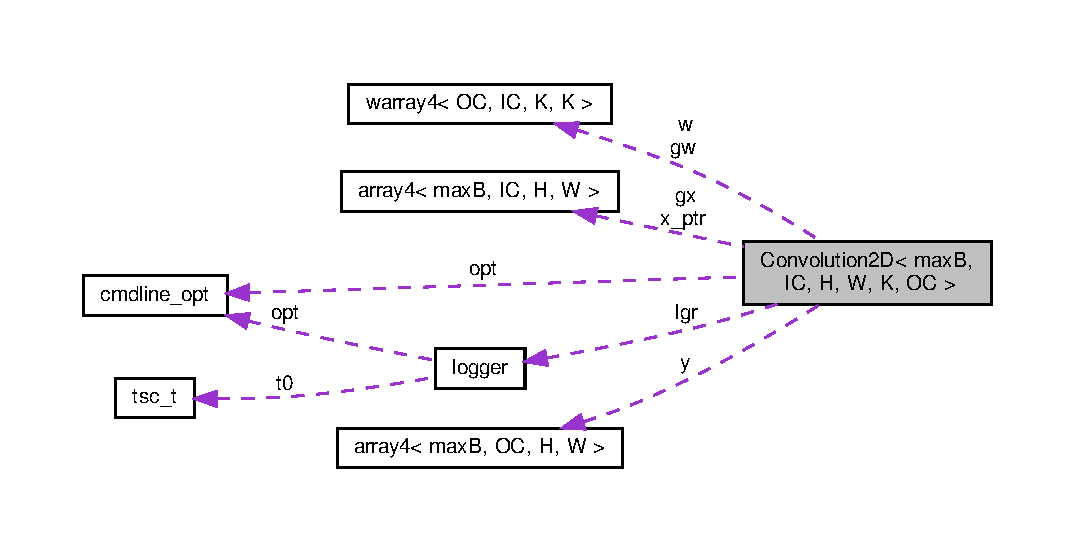
\includegraphics[width=350pt]{structConvolution2D__coll__graph}
\end{center}
\end{figure}
\subsection*{Public Member Functions}
\begin{DoxyCompactItemize}
\item 
void \hyperlink{structConvolution2D_aa3c6a51a0b4278dacf8dff4f80e86943}{init} (\hyperlink{structcmdline__opt}{cmdline\+\_\+opt} \hyperlink{structConvolution2D_ad873766a934a3589b2feec7933dc11f2}{opt}, \hyperlink{structlogger}{logger} $\ast$\hyperlink{structConvolution2D_a1c0363cbb527e0dcdb032a2b6b5ea9e6}{lgr}, \hyperlink{structrnd__gen__t}{rnd\+\_\+gen\+\_\+t} \&rg)
\begin{DoxyCompactList}\small\item\em initialize \end{DoxyCompactList}\item 
\hyperlink{structConvolution2D}{Convolution2D}$<$ maxB, IC, H, W, K, OC $>$ $\ast$ \hyperlink{structConvolution2D_aec12842fd665f7d7a0d6d68db68f4fed}{copy} ()
\begin{DoxyCompactList}\small\item\em make a copy of this \end{DoxyCompactList}\item 
void \hyperlink{structConvolution2D_a4e0dca3719249dbceb4afe64f8844f7f}{set\+\_\+dev} (\hyperlink{structConvolution2D}{Convolution2D}$<$ maxB, IC, H, W, K, OC $>$ $\ast$\hyperlink{structConvolution2D_a3b9891c27e266092619413a16518a9e9}{dev})
\begin{DoxyCompactList}\small\item\em set the device pointer for this and all subobjects \end{DoxyCompactList}\item 
void \hyperlink{structConvolution2D_a9c6908bf3797c1b38dec8c33beb8df49}{make\+\_\+dev} ()
\begin{DoxyCompactList}\small\item\em if the algorithm is a gpu algorithm, allocate a device shadow of this object and set dev field of this and all subobjects. otherwise it sets all dev fields to null. \end{DoxyCompactList}\item 
void \hyperlink{structConvolution2D_a3f508b68dc981593f5a2980e6b88a247}{del\+\_\+dev} ()
\begin{DoxyCompactList}\small\item\em if the algorithm is a gpu algorithm, dev field must not be null and deallocate it. \end{DoxyCompactList}\item 
\mbox{\Hypertarget{structConvolution2D_a325b68731e0c4f171785238ad406b549}\label{structConvolution2D_a325b68731e0c4f171785238ad406b549}} 
void \hyperlink{structConvolution2D_a325b68731e0c4f171785238ad406b549}{to\+\_\+dev} ()
\begin{DoxyCompactList}\small\item\em if the algorithm is a gpu algorithm, dev field must not be null and send the host data to the device memory \end{DoxyCompactList}\item 
\mbox{\Hypertarget{structConvolution2D_a65bda262ba5fed9c7bb87cbf6caf86ac}\label{structConvolution2D_a65bda262ba5fed9c7bb87cbf6caf86ac}} 
void \hyperlink{structConvolution2D_a65bda262ba5fed9c7bb87cbf6caf86ac}{to\+\_\+host} ()
\begin{DoxyCompactList}\small\item\em if the algorithm is a gpu algorithm, dev field must not be null and send the device data to the host memory \end{DoxyCompactList}\item 
\+\_\+\+\_\+device\+\_\+\+\_\+ \+\_\+\+\_\+host\+\_\+\+\_\+ void \hyperlink{structConvolution2D_a5134826f56423c7629434f4c9ea40a1f}{update\+\_\+base} (\hyperlink{vgg__util_8h_a1082d08aaa761215ec83e7149f27ad16}{real} eta)
\begin{DoxyCompactList}\small\item\em the baseline (serial) implementation of update called both by cpu implementation (update\+\_\+cpu) and gpu implementation (update\+\_\+dev). the call sequence update -\/$>$ update\+\_\+cpu -\/$>$ update\+\_\+base on cpu and and is update -\/$>$ update\+\_\+gpu -\/$>$ update\+\_\+global -\/$>$ update\+\_\+dev -\/$>$ update\+\_\+base \end{DoxyCompactList}\item 
\+\_\+\+\_\+device\+\_\+\+\_\+ void \hyperlink{structConvolution2D_a724e0e31fb47f11af0f022adf983ca41}{update\+\_\+dev} (\hyperlink{vgg__util_8h_a1082d08aaa761215ec83e7149f27ad16}{real} eta)
\begin{DoxyCompactList}\small\item\em the device function of update called from the global (non-\/member) function \end{DoxyCompactList}\item 
void \hyperlink{structConvolution2D_af189fb21ba3ecb6b9f7553c414f35446}{update\+\_\+gpu} (\hyperlink{vgg__util_8h_a1082d08aaa761215ec83e7149f27ad16}{real} eta)
\begin{DoxyCompactList}\small\item\em a gpu version of baseline code called from the entry function (update) \end{DoxyCompactList}\item 
void \hyperlink{structConvolution2D_a3768142c7d9dc9649b6afb1d2321449a}{update\+\_\+cpu} (\hyperlink{vgg__util_8h_a1082d08aaa761215ec83e7149f27ad16}{real} eta)
\begin{DoxyCompactList}\small\item\em a cpu version of baseline code called from the entry function (update) \end{DoxyCompactList}\item 
void \hyperlink{structConvolution2D_ac9fd666f96904bb7f62dc39cebae7a25}{update} (\hyperlink{vgg__util_8h_a1082d08aaa761215ec83e7149f27ad16}{real} eta)
\begin{DoxyCompactList}\small\item\em update weights of all sublayers with gradients that must have been computed \end{DoxyCompactList}\item 
\+\_\+\+\_\+device\+\_\+\+\_\+ \+\_\+\+\_\+host\+\_\+\+\_\+ void \hyperlink{structConvolution2D_aa969d35c6c2ca209354d3fd9249fcf82}{forward\+\_\+base} (\hyperlink{structarray4}{array4}$<$ maxB, IC, H, W $>$ \&x)
\begin{DoxyCompactList}\small\item\em the baseline (serial) implementation of forward called both by cpu implementation (forward\+\_\+cpu) and gpu implementation (forward\+\_\+dev). the call sequence forward -\/$>$ forward\+\_\+cpu -\/$>$ forward\+\_\+base on cpu and and is forward -\/$>$ forward\+\_\+gpu -\/$>$ forward\+\_\+global -\/$>$ forward\+\_\+dev -\/$>$ forward\+\_\+base \end{DoxyCompactList}\item 
\+\_\+\+\_\+device\+\_\+\+\_\+ void \hyperlink{structConvolution2D_a1e5d3b49b05f8444178be5f73f59bedd}{forward\+\_\+dev} (\hyperlink{structarray4}{array4}$<$ maxB, IC, H, W $>$ \&x)
\begin{DoxyCompactList}\small\item\em the device function of forward called from the global (non-\/member) function \end{DoxyCompactList}\item 
void \hyperlink{structConvolution2D_ac8bbdceed275bddaaf937e1b7ce2e5ac}{forward\+\_\+gpu} (\hyperlink{structarray4}{array4}$<$ maxB, IC, H, W $>$ \&x)
\begin{DoxyCompactList}\small\item\em a gpu version of baseline code called from the entry function (forward) \end{DoxyCompactList}\item 
void \hyperlink{structConvolution2D_ac1dcf1aebcf205c34bbf604d3b68562b}{forward\+\_\+cpu} (\hyperlink{structarray4}{array4}$<$ maxB, IC, H, W $>$ \&x)
\begin{DoxyCompactList}\small\item\em a cpu version of baseline code called from the entry function (forward) \end{DoxyCompactList}\item 
\hyperlink{structarray4}{array4}$<$ maxB, OC, H, W $>$ \& \hyperlink{structConvolution2D_ae6dcfaea38b779de24bbda730c57083e}{forward} (\hyperlink{structarray4}{array4}$<$ maxB, IC, H, W $>$ \&x)
\begin{DoxyCompactList}\small\item\em calc the loss function of a mini-\/batch (x) \end{DoxyCompactList}\item 
\+\_\+\+\_\+device\+\_\+\+\_\+ \+\_\+\+\_\+host\+\_\+\+\_\+ void \hyperlink{structConvolution2D_af202e85ae6c5aa5e4aae6869a8891fc3}{backward\+\_\+base} (\hyperlink{structarray4}{array4}$<$ maxB, OC, H, W $>$ \&gy)
\begin{DoxyCompactList}\small\item\em the baseline (serial) implementation of backward called both by cpu implementation (backward\+\_\+cpu) and gpu implementation (backward\+\_\+dev). the call sequence backward -\/$>$ backward\+\_\+cpu -\/$>$ backward\+\_\+base on cpu and and is backward -\/$>$ backward\+\_\+gpu -\/$>$ backward\+\_\+global -\/$>$ backward\+\_\+dev -\/$>$ backward\+\_\+base \end{DoxyCompactList}\item 
\+\_\+\+\_\+device\+\_\+\+\_\+ void \hyperlink{structConvolution2D_a144c8af173f1cbb9e7efade3b2f19f1e}{backward\+\_\+dev} (\hyperlink{structarray4}{array4}$<$ maxB, OC, H, W $>$ \&gy)
\begin{DoxyCompactList}\small\item\em the device function of backward called from the global (non-\/member) function \end{DoxyCompactList}\item 
void \hyperlink{structConvolution2D_af7105f910c11a7bd93e27a7abc06e502}{backward\+\_\+gpu} (\hyperlink{structarray4}{array4}$<$ maxB, OC, H, W $>$ \&gy)
\begin{DoxyCompactList}\small\item\em a gpu version of baseline code called from the entry function (backward) \end{DoxyCompactList}\item 
void \hyperlink{structConvolution2D_a8b9838267f044544073f95a278304f06}{backward\+\_\+cpu} (\hyperlink{structarray4}{array4}$<$ maxB, OC, H, W $>$ \&gy)
\begin{DoxyCompactList}\small\item\em a cpu version of baseline code called from the entry function (backward) \end{DoxyCompactList}\item 
\hyperlink{structarray4}{array4}$<$ maxB, IC, H, W $>$ \& \hyperlink{structConvolution2D_ace928f0589a42b6505f5787652ffbacd}{backward} (\hyperlink{structarray4}{array4}$<$ maxB, OC, H, W $>$ \&gy)
\begin{DoxyCompactList}\small\item\em calc the gradient of loss wrt the input (x) \end{DoxyCompactList}\item 
void \hyperlink{structConvolution2D_ac66223a9688f45e3422bbdd24c891f70}{rand\+\_\+grad} (\hyperlink{structrnd__gen__t}{rnd\+\_\+gen\+\_\+t} \&rg, \hyperlink{vgg__util_8h_a1082d08aaa761215ec83e7149f27ad16}{real} p, \hyperlink{vgg__util_8h_a1082d08aaa761215ec83e7149f27ad16}{real} q)
\begin{DoxyCompactList}\small\item\em randomly set all gradients to values between p and q \end{DoxyCompactList}\item 
void \hyperlink{structConvolution2D_a8b1f4363ec5f6d3d69890599a0e426da}{set\+\_\+grad} (\hyperlink{structConvolution2D}{Convolution2D}$<$ maxB, IC, H, W, K, OC $>$ \&o)
\begin{DoxyCompactList}\small\item\em set all gradients to gradients of another object \end{DoxyCompactList}\item 
\hyperlink{vgg__util_8h_a1082d08aaa761215ec83e7149f27ad16}{real} \hyperlink{structConvolution2D_a41442b7f48f34045660dbcd64301d14b}{gw\+\_\+dot\+\_\+gw} (\hyperlink{structConvolution2D}{Convolution2D}$<$ maxB, IC, H, W, K, OC $>$ \&o)
\begin{DoxyCompactList}\small\item\em take the inner product of gradients \end{DoxyCompactList}\end{DoxyCompactItemize}
\subsection*{Public Attributes}
\begin{DoxyCompactItemize}
\item 
\hyperlink{structConvolution2D}{Convolution2D}$<$ maxB, IC, H, W, K, OC $>$ $\ast$ \hyperlink{structConvolution2D_a3b9891c27e266092619413a16518a9e9}{dev}
\item 
\hyperlink{structcmdline__opt}{cmdline\+\_\+opt} \hyperlink{structConvolution2D_ad873766a934a3589b2feec7933dc11f2}{opt}
\item 
\hyperlink{structlogger}{logger} $\ast$ \hyperlink{structConvolution2D_a1c0363cbb527e0dcdb032a2b6b5ea9e6}{lgr}
\item 
\hyperlink{structarray4}{array4}$<$ maxB, IC, H, W $>$ $\ast$ \hyperlink{structConvolution2D_a404b6e9b9a932e463f237d5bd35b2154}{x\+\_\+ptr}
\item 
\hyperlink{structwarray4}{warray4}$<$ OC, IC, K, K $>$ \hyperlink{structConvolution2D_a20027e8ac911e6ec9db15a7ecaf4a16a}{w}
\item 
\hyperlink{structarray4}{array4}$<$ maxB, OC, H, W $>$ \hyperlink{structConvolution2D_ae321933a802088a32112cdbd16b16c0f}{y}
\item 
\hyperlink{structwarray4}{warray4}$<$ OC, IC, K, K $>$ \hyperlink{structConvolution2D_acbd8375eef9aa08bd061b3898dbdc403}{gw}
\item 
\hyperlink{structarray4}{array4}$<$ maxB, IC, H, W $>$ \hyperlink{structConvolution2D_a1bc2147fc750b2587a82d865eef24d2c}{gx}
\end{DoxyCompactItemize}


\subsection{Detailed Description}
\subsubsection*{template$<$idx\+\_\+t maxB, idx\+\_\+t IC, idx\+\_\+t H, idx\+\_\+t W, idx\+\_\+t K, idx\+\_\+t OC$>$\newline
struct Convolution2\+D$<$ max\+B, I\+C, H, W, K, O\+C $>$}

convolution of images 


\begin{DoxyParams}{Parameters}
{\em (max\+B)} & the maximum number of images (batch size) \\
\hline
{\em (\+I\+C)} & the number of channels per input image (the original input has typically three channels for R\+GB. in hidden layers, it starts from 64 and goes up to 512 in the last hidden layer) \\
\hline
{\em (\+H)} & height of an image (32 for an input image, down to 1 in the last hidden layer) \\
\hline
{\em (\+W)} & width of an image (32 for an input image, down to 1 in the last hidden layer) \\
\hline
{\em (\+K)} & convolution kernel size (1). filter array has (2\+K+1)$\ast$(2\+K+1) elems) \\
\hline
{\em (\+O\+C)} & the number of channels per an output image\\
\hline
\end{DoxyParams}
this layer converts each I\+Cx\+WxH image to O\+Cx\+WxH image, applying I\+Cx(2\+K+1)x(2\+K+1) stencil to each pixel 

\subsection{Member Function Documentation}
\mbox{\Hypertarget{structConvolution2D_ace928f0589a42b6505f5787652ffbacd}\label{structConvolution2D_ace928f0589a42b6505f5787652ffbacd}} 
\index{Convolution2D@{Convolution2D}!backward@{backward}}
\index{backward@{backward}!Convolution2D@{Convolution2D}}
\subsubsection{\texorpdfstring{backward()}{backward()}}
{\footnotesize\ttfamily template$<$idx\+\_\+t maxB, idx\+\_\+t IC, idx\+\_\+t H, idx\+\_\+t W, idx\+\_\+t K, idx\+\_\+t OC$>$ \\
\hyperlink{structarray4}{array4}$<$maxB,IC,H,W$>$\& \hyperlink{structConvolution2D}{Convolution2D}$<$ maxB, IC, H, W, K, OC $>$\+::backward (\begin{DoxyParamCaption}\item[{\hyperlink{structarray4}{array4}$<$ maxB, OC, H, W $>$ \&}]{gy }\end{DoxyParamCaption})\hspace{0.3cm}{\ttfamily [inline]}}



calc the gradient of loss wrt the input (x) 


\begin{DoxyParams}{Parameters}
{\em (gy)} & gradient of loss with respect to the output\\
\hline
\end{DoxyParams}
calc the gradient of loss wrt the input. along the way, it also calculates the gradient of loss wrt weights for all sublayers that have weights. since this is the entire network, gy is actually a vector whose components are all 1. (loss = sum of losses of each data). \begin{DoxySeeAlso}{See also}
\hyperlink{structConvolution2D_ae6dcfaea38b779de24bbda730c57083e}{forward} 

\hyperlink{structConvolution2D_ac9fd666f96904bb7f62dc39cebae7a25}{update} 
\end{DoxySeeAlso}
\mbox{\Hypertarget{structConvolution2D_af202e85ae6c5aa5e4aae6869a8891fc3}\label{structConvolution2D_af202e85ae6c5aa5e4aae6869a8891fc3}} 
\index{Convolution2D@{Convolution2D}!backward\+\_\+base@{backward\+\_\+base}}
\index{backward\+\_\+base@{backward\+\_\+base}!Convolution2D@{Convolution2D}}
\subsubsection{\texorpdfstring{backward\+\_\+base()}{backward\_base()}}
{\footnotesize\ttfamily template$<$idx\+\_\+t maxB, idx\+\_\+t IC, idx\+\_\+t H, idx\+\_\+t W, idx\+\_\+t K, idx\+\_\+t OC$>$ \\
\+\_\+\+\_\+device\+\_\+\+\_\+ \+\_\+\+\_\+host\+\_\+\+\_\+ void \hyperlink{structConvolution2D}{Convolution2D}$<$ maxB, IC, H, W, K, OC $>$\+::backward\+\_\+base (\begin{DoxyParamCaption}\item[{\hyperlink{structarray4}{array4}$<$ maxB, OC, H, W $>$ \&}]{gy }\end{DoxyParamCaption})\hspace{0.3cm}{\ttfamily [inline]}}



the baseline (serial) implementation of backward called both by cpu implementation (backward\+\_\+cpu) and gpu implementation (backward\+\_\+dev). the call sequence backward -\/$>$ backward\+\_\+cpu -\/$>$ backward\+\_\+base on cpu and and is backward -\/$>$ backward\+\_\+gpu -\/$>$ backward\+\_\+global -\/$>$ backward\+\_\+dev -\/$>$ backward\+\_\+base 


\begin{DoxyParams}{Parameters}
{\em (gy)} & gradient of loss with respect to the output \\
\hline
\end{DoxyParams}
\begin{DoxySeeAlso}{See also}
\hyperlink{structConvolution2D_ace928f0589a42b6505f5787652ffbacd}{backward} 

\hyperlink{structConvolution2D_af7105f910c11a7bd93e27a7abc06e502}{backward\+\_\+gpu} 

\hyperlink{softmaxcrossentropy_8h_a47d56a9a23e08247b227f4aac17413e0}{backward\+\_\+global} 

\hyperlink{structConvolution2D_a144c8af173f1cbb9e7efade3b2f19f1e}{backward\+\_\+dev} 
\end{DoxySeeAlso}
\mbox{\Hypertarget{structConvolution2D_a8b9838267f044544073f95a278304f06}\label{structConvolution2D_a8b9838267f044544073f95a278304f06}} 
\index{Convolution2D@{Convolution2D}!backward\+\_\+cpu@{backward\+\_\+cpu}}
\index{backward\+\_\+cpu@{backward\+\_\+cpu}!Convolution2D@{Convolution2D}}
\subsubsection{\texorpdfstring{backward\+\_\+cpu()}{backward\_cpu()}}
{\footnotesize\ttfamily template$<$idx\+\_\+t maxB, idx\+\_\+t IC, idx\+\_\+t H, idx\+\_\+t W, idx\+\_\+t K, idx\+\_\+t OC$>$ \\
void \hyperlink{structConvolution2D}{Convolution2D}$<$ maxB, IC, H, W, K, OC $>$\+::backward\+\_\+cpu (\begin{DoxyParamCaption}\item[{\hyperlink{structarray4}{array4}$<$ maxB, OC, H, W $>$ \&}]{gy }\end{DoxyParamCaption})\hspace{0.3cm}{\ttfamily [inline]}}



a cpu version of baseline code called from the entry function (backward) 


\begin{DoxyParams}{Parameters}
{\em (gy)} & gradient of loss with respect to the output \\
\hline
\end{DoxyParams}
\begin{DoxySeeAlso}{See also}
\hyperlink{structConvolution2D_ace928f0589a42b6505f5787652ffbacd}{backward} 

\hyperlink{structConvolution2D_af202e85ae6c5aa5e4aae6869a8891fc3}{backward\+\_\+base} 
\end{DoxySeeAlso}
\mbox{\Hypertarget{structConvolution2D_a144c8af173f1cbb9e7efade3b2f19f1e}\label{structConvolution2D_a144c8af173f1cbb9e7efade3b2f19f1e}} 
\index{Convolution2D@{Convolution2D}!backward\+\_\+dev@{backward\+\_\+dev}}
\index{backward\+\_\+dev@{backward\+\_\+dev}!Convolution2D@{Convolution2D}}
\subsubsection{\texorpdfstring{backward\+\_\+dev()}{backward\_dev()}}
{\footnotesize\ttfamily template$<$idx\+\_\+t maxB, idx\+\_\+t IC, idx\+\_\+t H, idx\+\_\+t W, idx\+\_\+t K, idx\+\_\+t OC$>$ \\
\+\_\+\+\_\+device\+\_\+\+\_\+ void \hyperlink{structConvolution2D}{Convolution2D}$<$ maxB, IC, H, W, K, OC $>$\+::backward\+\_\+dev (\begin{DoxyParamCaption}\item[{\hyperlink{structarray4}{array4}$<$ maxB, OC, H, W $>$ \&}]{gy }\end{DoxyParamCaption})\hspace{0.3cm}{\ttfamily [inline]}}



the device function of backward called from the global (non-\/member) function 


\begin{DoxyParams}{Parameters}
{\em (gy)} & gradient of loss with respect to the output \\
\hline
\end{DoxyParams}
\begin{DoxySeeAlso}{See also}
\hyperlink{structConvolution2D_ace928f0589a42b6505f5787652ffbacd}{backward} 

\hyperlink{structConvolution2D_af7105f910c11a7bd93e27a7abc06e502}{backward\+\_\+gpu} 

\hyperlink{softmaxcrossentropy_8h_a47d56a9a23e08247b227f4aac17413e0}{backward\+\_\+global} 

\hyperlink{structConvolution2D_af202e85ae6c5aa5e4aae6869a8891fc3}{backward\+\_\+base} 
\end{DoxySeeAlso}
\mbox{\Hypertarget{structConvolution2D_af7105f910c11a7bd93e27a7abc06e502}\label{structConvolution2D_af7105f910c11a7bd93e27a7abc06e502}} 
\index{Convolution2D@{Convolution2D}!backward\+\_\+gpu@{backward\+\_\+gpu}}
\index{backward\+\_\+gpu@{backward\+\_\+gpu}!Convolution2D@{Convolution2D}}
\subsubsection{\texorpdfstring{backward\+\_\+gpu()}{backward\_gpu()}}
{\footnotesize\ttfamily template$<$idx\+\_\+t maxB, idx\+\_\+t IC, idx\+\_\+t H, idx\+\_\+t W, idx\+\_\+t K, idx\+\_\+t OC$>$ \\
void \hyperlink{structConvolution2D}{Convolution2D}$<$ maxB, IC, H, W, K, OC $>$\+::backward\+\_\+gpu (\begin{DoxyParamCaption}\item[{\hyperlink{structarray4}{array4}$<$ maxB, OC, H, W $>$ \&}]{gy }\end{DoxyParamCaption})\hspace{0.3cm}{\ttfamily [inline]}}



a gpu version of baseline code called from the entry function (backward) 


\begin{DoxyParams}{Parameters}
{\em (gy)} & gradient of loss with respect to the output \\
\hline
\end{DoxyParams}
\begin{DoxySeeAlso}{See also}
\hyperlink{structConvolution2D_ace928f0589a42b6505f5787652ffbacd}{backward} 

\hyperlink{softmaxcrossentropy_8h_a47d56a9a23e08247b227f4aac17413e0}{backward\+\_\+global} 

\hyperlink{structConvolution2D_a144c8af173f1cbb9e7efade3b2f19f1e}{backward\+\_\+dev} 

\hyperlink{structConvolution2D_af202e85ae6c5aa5e4aae6869a8891fc3}{backward\+\_\+base} 
\end{DoxySeeAlso}
\mbox{\Hypertarget{structConvolution2D_aec12842fd665f7d7a0d6d68db68f4fed}\label{structConvolution2D_aec12842fd665f7d7a0d6d68db68f4fed}} 
\index{Convolution2D@{Convolution2D}!copy@{copy}}
\index{copy@{copy}!Convolution2D@{Convolution2D}}
\subsubsection{\texorpdfstring{copy()}{copy()}}
{\footnotesize\ttfamily template$<$idx\+\_\+t maxB, idx\+\_\+t IC, idx\+\_\+t H, idx\+\_\+t W, idx\+\_\+t K, idx\+\_\+t OC$>$ \\
\hyperlink{structConvolution2D}{Convolution2D}$<$maxB,IC,H,W,K,OC$>$$\ast$ \hyperlink{structConvolution2D}{Convolution2D}$<$ maxB, IC, H, W, K, OC $>$\+::copy (\begin{DoxyParamCaption}{ }\end{DoxyParamCaption})\hspace{0.3cm}{\ttfamily [inline]}}



make a copy of this 

if this object has a device pointer, the copy will have a device pointer too, but its contents are N\+OT copied \mbox{\Hypertarget{structConvolution2D_a3f508b68dc981593f5a2980e6b88a247}\label{structConvolution2D_a3f508b68dc981593f5a2980e6b88a247}} 
\index{Convolution2D@{Convolution2D}!del\+\_\+dev@{del\+\_\+dev}}
\index{del\+\_\+dev@{del\+\_\+dev}!Convolution2D@{Convolution2D}}
\subsubsection{\texorpdfstring{del\+\_\+dev()}{del\_dev()}}
{\footnotesize\ttfamily template$<$idx\+\_\+t maxB, idx\+\_\+t IC, idx\+\_\+t H, idx\+\_\+t W, idx\+\_\+t K, idx\+\_\+t OC$>$ \\
void \hyperlink{structConvolution2D}{Convolution2D}$<$ maxB, IC, H, W, K, OC $>$\+::del\+\_\+dev (\begin{DoxyParamCaption}{ }\end{DoxyParamCaption})\hspace{0.3cm}{\ttfamily [inline]}}



if the algorithm is a gpu algorithm, dev field must not be null and deallocate it. 

\begin{DoxySeeAlso}{See also}
\hyperlink{structConvolution2D_a9c6908bf3797c1b38dec8c33beb8df49}{make\+\_\+dev} 

\hyperlink{structConvolution2D_a4e0dca3719249dbceb4afe64f8844f7f}{set\+\_\+dev} 
\end{DoxySeeAlso}
\mbox{\Hypertarget{structConvolution2D_ae6dcfaea38b779de24bbda730c57083e}\label{structConvolution2D_ae6dcfaea38b779de24bbda730c57083e}} 
\index{Convolution2D@{Convolution2D}!forward@{forward}}
\index{forward@{forward}!Convolution2D@{Convolution2D}}
\subsubsection{\texorpdfstring{forward()}{forward()}}
{\footnotesize\ttfamily template$<$idx\+\_\+t maxB, idx\+\_\+t IC, idx\+\_\+t H, idx\+\_\+t W, idx\+\_\+t K, idx\+\_\+t OC$>$ \\
\hyperlink{structarray4}{array4}$<$maxB,OC,H,W$>$\& \hyperlink{structConvolution2D}{Convolution2D}$<$ maxB, IC, H, W, K, OC $>$\+::forward (\begin{DoxyParamCaption}\item[{\hyperlink{structarray4}{array4}$<$ maxB, IC, H, W $>$ \&}]{x }\end{DoxyParamCaption})\hspace{0.3cm}{\ttfamily [inline]}}



calc the loss function of a mini-\/batch (x) 


\begin{DoxyParams}{Parameters}
{\em (x)} & input images \\
\hline
\end{DoxyParams}
\begin{DoxySeeAlso}{See also}
\hyperlink{structConvolution2D_ace928f0589a42b6505f5787652ffbacd}{backward} 

\hyperlink{structConvolution2D_ac9fd666f96904bb7f62dc39cebae7a25}{update} 
\end{DoxySeeAlso}
\mbox{\Hypertarget{structConvolution2D_aa969d35c6c2ca209354d3fd9249fcf82}\label{structConvolution2D_aa969d35c6c2ca209354d3fd9249fcf82}} 
\index{Convolution2D@{Convolution2D}!forward\+\_\+base@{forward\+\_\+base}}
\index{forward\+\_\+base@{forward\+\_\+base}!Convolution2D@{Convolution2D}}
\subsubsection{\texorpdfstring{forward\+\_\+base()}{forward\_base()}}
{\footnotesize\ttfamily template$<$idx\+\_\+t maxB, idx\+\_\+t IC, idx\+\_\+t H, idx\+\_\+t W, idx\+\_\+t K, idx\+\_\+t OC$>$ \\
\+\_\+\+\_\+device\+\_\+\+\_\+ \+\_\+\+\_\+host\+\_\+\+\_\+ void \hyperlink{structConvolution2D}{Convolution2D}$<$ maxB, IC, H, W, K, OC $>$\+::forward\+\_\+base (\begin{DoxyParamCaption}\item[{\hyperlink{structarray4}{array4}$<$ maxB, IC, H, W $>$ \&}]{x }\end{DoxyParamCaption})\hspace{0.3cm}{\ttfamily [inline]}}



the baseline (serial) implementation of forward called both by cpu implementation (forward\+\_\+cpu) and gpu implementation (forward\+\_\+dev). the call sequence forward -\/$>$ forward\+\_\+cpu -\/$>$ forward\+\_\+base on cpu and and is forward -\/$>$ forward\+\_\+gpu -\/$>$ forward\+\_\+global -\/$>$ forward\+\_\+dev -\/$>$ forward\+\_\+base 


\begin{DoxyParams}{Parameters}
{\em (x)} & input images \\
\hline
\end{DoxyParams}
\begin{DoxySeeAlso}{See also}
\hyperlink{structConvolution2D_ae6dcfaea38b779de24bbda730c57083e}{forward} 

\hyperlink{structConvolution2D_ac8bbdceed275bddaaf937e1b7ce2e5ac}{forward\+\_\+gpu} 

\hyperlink{softmaxcrossentropy_8h_a578aeeb166bd06e800d9b396eab48b35}{forward\+\_\+global} 

\hyperlink{structConvolution2D_a1e5d3b49b05f8444178be5f73f59bedd}{forward\+\_\+dev} 
\end{DoxySeeAlso}
\mbox{\Hypertarget{structConvolution2D_ac1dcf1aebcf205c34bbf604d3b68562b}\label{structConvolution2D_ac1dcf1aebcf205c34bbf604d3b68562b}} 
\index{Convolution2D@{Convolution2D}!forward\+\_\+cpu@{forward\+\_\+cpu}}
\index{forward\+\_\+cpu@{forward\+\_\+cpu}!Convolution2D@{Convolution2D}}
\subsubsection{\texorpdfstring{forward\+\_\+cpu()}{forward\_cpu()}}
{\footnotesize\ttfamily template$<$idx\+\_\+t maxB, idx\+\_\+t IC, idx\+\_\+t H, idx\+\_\+t W, idx\+\_\+t K, idx\+\_\+t OC$>$ \\
void \hyperlink{structConvolution2D}{Convolution2D}$<$ maxB, IC, H, W, K, OC $>$\+::forward\+\_\+cpu (\begin{DoxyParamCaption}\item[{\hyperlink{structarray4}{array4}$<$ maxB, IC, H, W $>$ \&}]{x }\end{DoxyParamCaption})\hspace{0.3cm}{\ttfamily [inline]}}



a cpu version of baseline code called from the entry function (forward) 


\begin{DoxyParams}{Parameters}
{\em (x)} & input images \\
\hline
\end{DoxyParams}
\begin{DoxySeeAlso}{See also}
\hyperlink{structConvolution2D_ae6dcfaea38b779de24bbda730c57083e}{forward} 

\hyperlink{structConvolution2D_aa969d35c6c2ca209354d3fd9249fcf82}{forward\+\_\+base} 
\end{DoxySeeAlso}
\mbox{\Hypertarget{structConvolution2D_a1e5d3b49b05f8444178be5f73f59bedd}\label{structConvolution2D_a1e5d3b49b05f8444178be5f73f59bedd}} 
\index{Convolution2D@{Convolution2D}!forward\+\_\+dev@{forward\+\_\+dev}}
\index{forward\+\_\+dev@{forward\+\_\+dev}!Convolution2D@{Convolution2D}}
\subsubsection{\texorpdfstring{forward\+\_\+dev()}{forward\_dev()}}
{\footnotesize\ttfamily template$<$idx\+\_\+t maxB, idx\+\_\+t IC, idx\+\_\+t H, idx\+\_\+t W, idx\+\_\+t K, idx\+\_\+t OC$>$ \\
\+\_\+\+\_\+device\+\_\+\+\_\+ void \hyperlink{structConvolution2D}{Convolution2D}$<$ maxB, IC, H, W, K, OC $>$\+::forward\+\_\+dev (\begin{DoxyParamCaption}\item[{\hyperlink{structarray4}{array4}$<$ maxB, IC, H, W $>$ \&}]{x }\end{DoxyParamCaption})\hspace{0.3cm}{\ttfamily [inline]}}



the device function of forward called from the global (non-\/member) function 


\begin{DoxyParams}{Parameters}
{\em (x)} & input images \\
\hline
\end{DoxyParams}
\begin{DoxySeeAlso}{See also}
\hyperlink{structConvolution2D_ae6dcfaea38b779de24bbda730c57083e}{forward} 

\hyperlink{structConvolution2D_ac8bbdceed275bddaaf937e1b7ce2e5ac}{forward\+\_\+gpu} 

\hyperlink{softmaxcrossentropy_8h_a578aeeb166bd06e800d9b396eab48b35}{forward\+\_\+global} 

\hyperlink{structConvolution2D_aa969d35c6c2ca209354d3fd9249fcf82}{forward\+\_\+base} 
\end{DoxySeeAlso}
\mbox{\Hypertarget{structConvolution2D_ac8bbdceed275bddaaf937e1b7ce2e5ac}\label{structConvolution2D_ac8bbdceed275bddaaf937e1b7ce2e5ac}} 
\index{Convolution2D@{Convolution2D}!forward\+\_\+gpu@{forward\+\_\+gpu}}
\index{forward\+\_\+gpu@{forward\+\_\+gpu}!Convolution2D@{Convolution2D}}
\subsubsection{\texorpdfstring{forward\+\_\+gpu()}{forward\_gpu()}}
{\footnotesize\ttfamily template$<$idx\+\_\+t maxB, idx\+\_\+t IC, idx\+\_\+t H, idx\+\_\+t W, idx\+\_\+t K, idx\+\_\+t OC$>$ \\
void \hyperlink{structConvolution2D}{Convolution2D}$<$ maxB, IC, H, W, K, OC $>$\+::forward\+\_\+gpu (\begin{DoxyParamCaption}\item[{\hyperlink{structarray4}{array4}$<$ maxB, IC, H, W $>$ \&}]{x }\end{DoxyParamCaption})\hspace{0.3cm}{\ttfamily [inline]}}



a gpu version of baseline code called from the entry function (forward) 


\begin{DoxyParams}{Parameters}
{\em (x)} & input images \\
\hline
\end{DoxyParams}
\begin{DoxySeeAlso}{See also}
\hyperlink{structConvolution2D_ae6dcfaea38b779de24bbda730c57083e}{forward} 

\hyperlink{softmaxcrossentropy_8h_a578aeeb166bd06e800d9b396eab48b35}{forward\+\_\+global} 

\hyperlink{structConvolution2D_a1e5d3b49b05f8444178be5f73f59bedd}{forward\+\_\+dev} 

\hyperlink{structConvolution2D_aa969d35c6c2ca209354d3fd9249fcf82}{forward\+\_\+base} 
\end{DoxySeeAlso}
\mbox{\Hypertarget{structConvolution2D_a41442b7f48f34045660dbcd64301d14b}\label{structConvolution2D_a41442b7f48f34045660dbcd64301d14b}} 
\index{Convolution2D@{Convolution2D}!gw\+\_\+dot\+\_\+gw@{gw\+\_\+dot\+\_\+gw}}
\index{gw\+\_\+dot\+\_\+gw@{gw\+\_\+dot\+\_\+gw}!Convolution2D@{Convolution2D}}
\subsubsection{\texorpdfstring{gw\+\_\+dot\+\_\+gw()}{gw\_dot\_gw()}}
{\footnotesize\ttfamily template$<$idx\+\_\+t maxB, idx\+\_\+t IC, idx\+\_\+t H, idx\+\_\+t W, idx\+\_\+t K, idx\+\_\+t OC$>$ \\
\hyperlink{vgg__util_8h_a1082d08aaa761215ec83e7149f27ad16}{real} \hyperlink{structConvolution2D}{Convolution2D}$<$ maxB, IC, H, W, K, OC $>$\+::gw\+\_\+dot\+\_\+gw (\begin{DoxyParamCaption}\item[{\hyperlink{structConvolution2D}{Convolution2D}$<$ maxB, IC, H, W, K, OC $>$ \&}]{o }\end{DoxyParamCaption})\hspace{0.3cm}{\ttfamily [inline]}}



take the inner product of gradients 


\begin{DoxyParams}{Parameters}
{\em (o)} & the object to take the inner product with\\
\hline
\end{DoxyParams}
take the inner product of this object\textquotesingle{}s gradients and b\textquotesingle{}s gradients \mbox{\Hypertarget{structConvolution2D_aa3c6a51a0b4278dacf8dff4f80e86943}\label{structConvolution2D_aa3c6a51a0b4278dacf8dff4f80e86943}} 
\index{Convolution2D@{Convolution2D}!init@{init}}
\index{init@{init}!Convolution2D@{Convolution2D}}
\subsubsection{\texorpdfstring{init()}{init()}}
{\footnotesize\ttfamily template$<$idx\+\_\+t maxB, idx\+\_\+t IC, idx\+\_\+t H, idx\+\_\+t W, idx\+\_\+t K, idx\+\_\+t OC$>$ \\
void \hyperlink{structConvolution2D}{Convolution2D}$<$ maxB, IC, H, W, K, OC $>$\+::init (\begin{DoxyParamCaption}\item[{\hyperlink{structcmdline__opt}{cmdline\+\_\+opt}}]{opt,  }\item[{\hyperlink{structlogger}{logger} $\ast$}]{lgr,  }\item[{\hyperlink{structrnd__gen__t}{rnd\+\_\+gen\+\_\+t} \&}]{rg }\end{DoxyParamCaption})\hspace{0.3cm}{\ttfamily [inline]}}



initialize 


\begin{DoxyParams}{Parameters}
{\em (opt)} & command line options \\
\hline
{\em (lgr)} & logger \\
\hline
{\em (rg)} & random number generator for initializing weights \\
\hline
\end{DoxyParams}
\mbox{\Hypertarget{structConvolution2D_a9c6908bf3797c1b38dec8c33beb8df49}\label{structConvolution2D_a9c6908bf3797c1b38dec8c33beb8df49}} 
\index{Convolution2D@{Convolution2D}!make\+\_\+dev@{make\+\_\+dev}}
\index{make\+\_\+dev@{make\+\_\+dev}!Convolution2D@{Convolution2D}}
\subsubsection{\texorpdfstring{make\+\_\+dev()}{make\_dev()}}
{\footnotesize\ttfamily template$<$idx\+\_\+t maxB, idx\+\_\+t IC, idx\+\_\+t H, idx\+\_\+t W, idx\+\_\+t K, idx\+\_\+t OC$>$ \\
void \hyperlink{structConvolution2D}{Convolution2D}$<$ maxB, IC, H, W, K, OC $>$\+::make\+\_\+dev (\begin{DoxyParamCaption}{ }\end{DoxyParamCaption})\hspace{0.3cm}{\ttfamily [inline]}}



if the algorithm is a gpu algorithm, allocate a device shadow of this object and set dev field of this and all subobjects. otherwise it sets all dev fields to null. 

\begin{DoxySeeAlso}{See also}
\hyperlink{structConvolution2D_a4e0dca3719249dbceb4afe64f8844f7f}{set\+\_\+dev} 

\hyperlink{structConvolution2D_a3f508b68dc981593f5a2980e6b88a247}{del\+\_\+dev} 
\end{DoxySeeAlso}
\mbox{\Hypertarget{structConvolution2D_ac66223a9688f45e3422bbdd24c891f70}\label{structConvolution2D_ac66223a9688f45e3422bbdd24c891f70}} 
\index{Convolution2D@{Convolution2D}!rand\+\_\+grad@{rand\+\_\+grad}}
\index{rand\+\_\+grad@{rand\+\_\+grad}!Convolution2D@{Convolution2D}}
\subsubsection{\texorpdfstring{rand\+\_\+grad()}{rand\_grad()}}
{\footnotesize\ttfamily template$<$idx\+\_\+t maxB, idx\+\_\+t IC, idx\+\_\+t H, idx\+\_\+t W, idx\+\_\+t K, idx\+\_\+t OC$>$ \\
void \hyperlink{structConvolution2D}{Convolution2D}$<$ maxB, IC, H, W, K, OC $>$\+::rand\+\_\+grad (\begin{DoxyParamCaption}\item[{\hyperlink{structrnd__gen__t}{rnd\+\_\+gen\+\_\+t} \&}]{rg,  }\item[{\hyperlink{vgg__util_8h_a1082d08aaa761215ec83e7149f27ad16}{real}}]{p,  }\item[{\hyperlink{vgg__util_8h_a1082d08aaa761215ec83e7149f27ad16}{real}}]{q }\end{DoxyParamCaption})\hspace{0.3cm}{\ttfamily [inline]}}



randomly set all gradients to values between p and q 


\begin{DoxyParams}{Parameters}
{\em (rg)} & random number generator \\
\hline
{\em (p)} & minimum value of a component \\
\hline
{\em (q)} & maximum value of a component \\
\hline
\end{DoxyParams}
\mbox{\Hypertarget{structConvolution2D_a4e0dca3719249dbceb4afe64f8844f7f}\label{structConvolution2D_a4e0dca3719249dbceb4afe64f8844f7f}} 
\index{Convolution2D@{Convolution2D}!set\+\_\+dev@{set\+\_\+dev}}
\index{set\+\_\+dev@{set\+\_\+dev}!Convolution2D@{Convolution2D}}
\subsubsection{\texorpdfstring{set\+\_\+dev()}{set\_dev()}}
{\footnotesize\ttfamily template$<$idx\+\_\+t maxB, idx\+\_\+t IC, idx\+\_\+t H, idx\+\_\+t W, idx\+\_\+t K, idx\+\_\+t OC$>$ \\
void \hyperlink{structConvolution2D}{Convolution2D}$<$ maxB, IC, H, W, K, OC $>$\+::set\+\_\+dev (\begin{DoxyParamCaption}\item[{\hyperlink{structConvolution2D}{Convolution2D}$<$ maxB, IC, H, W, K, OC $>$ $\ast$}]{dev }\end{DoxyParamCaption})\hspace{0.3cm}{\ttfamily [inline]}}



set the device pointer for this and all subobjects 


\begin{DoxyParams}{Parameters}
{\em (dev)} & a device memory or null \\
\hline
\end{DoxyParams}
\begin{DoxySeeAlso}{See also}
\hyperlink{structConvolution2D_a9c6908bf3797c1b38dec8c33beb8df49}{make\+\_\+dev} 

\hyperlink{structConvolution2D_a3f508b68dc981593f5a2980e6b88a247}{del\+\_\+dev}
\end{DoxySeeAlso}
if dev is not null, dev fields of all subojects point to the corresponding subjects in the device memory. if dev is not null, all dev fields become null. \mbox{\Hypertarget{structConvolution2D_a8b1f4363ec5f6d3d69890599a0e426da}\label{structConvolution2D_a8b1f4363ec5f6d3d69890599a0e426da}} 
\index{Convolution2D@{Convolution2D}!set\+\_\+grad@{set\+\_\+grad}}
\index{set\+\_\+grad@{set\+\_\+grad}!Convolution2D@{Convolution2D}}
\subsubsection{\texorpdfstring{set\+\_\+grad()}{set\_grad()}}
{\footnotesize\ttfamily template$<$idx\+\_\+t maxB, idx\+\_\+t IC, idx\+\_\+t H, idx\+\_\+t W, idx\+\_\+t K, idx\+\_\+t OC$>$ \\
void \hyperlink{structConvolution2D}{Convolution2D}$<$ maxB, IC, H, W, K, OC $>$\+::set\+\_\+grad (\begin{DoxyParamCaption}\item[{\hyperlink{structConvolution2D}{Convolution2D}$<$ maxB, IC, H, W, K, OC $>$ \&}]{o }\end{DoxyParamCaption})\hspace{0.3cm}{\ttfamily [inline]}}



set all gradients to gradients of another object 


\begin{DoxyParams}{Parameters}
{\em (o)} & the object from which gradients get copied\\
\hline
\end{DoxyParams}
transfer gradients of o to this object \mbox{\Hypertarget{structConvolution2D_ac9fd666f96904bb7f62dc39cebae7a25}\label{structConvolution2D_ac9fd666f96904bb7f62dc39cebae7a25}} 
\index{Convolution2D@{Convolution2D}!update@{update}}
\index{update@{update}!Convolution2D@{Convolution2D}}
\subsubsection{\texorpdfstring{update()}{update()}}
{\footnotesize\ttfamily template$<$idx\+\_\+t maxB, idx\+\_\+t IC, idx\+\_\+t H, idx\+\_\+t W, idx\+\_\+t K, idx\+\_\+t OC$>$ \\
void \hyperlink{structConvolution2D}{Convolution2D}$<$ maxB, IC, H, W, K, OC $>$\+::update (\begin{DoxyParamCaption}\item[{\hyperlink{vgg__util_8h_a1082d08aaa761215ec83e7149f27ad16}{real}}]{eta }\end{DoxyParamCaption})\hspace{0.3cm}{\ttfamily [inline]}}



update weights of all sublayers with gradients that must have been computed 


\begin{DoxyParams}{Parameters}
{\em (eta)} & the learning rate \\
\hline
\end{DoxyParams}
\begin{DoxySeeAlso}{See also}
\hyperlink{structConvolution2D_ae6dcfaea38b779de24bbda730c57083e}{forward} 

\hyperlink{structConvolution2D_ace928f0589a42b6505f5787652ffbacd}{backward} 
\end{DoxySeeAlso}
\mbox{\Hypertarget{structConvolution2D_a5134826f56423c7629434f4c9ea40a1f}\label{structConvolution2D_a5134826f56423c7629434f4c9ea40a1f}} 
\index{Convolution2D@{Convolution2D}!update\+\_\+base@{update\+\_\+base}}
\index{update\+\_\+base@{update\+\_\+base}!Convolution2D@{Convolution2D}}
\subsubsection{\texorpdfstring{update\+\_\+base()}{update\_base()}}
{\footnotesize\ttfamily template$<$idx\+\_\+t maxB, idx\+\_\+t IC, idx\+\_\+t H, idx\+\_\+t W, idx\+\_\+t K, idx\+\_\+t OC$>$ \\
\+\_\+\+\_\+device\+\_\+\+\_\+ \+\_\+\+\_\+host\+\_\+\+\_\+ void \hyperlink{structConvolution2D}{Convolution2D}$<$ maxB, IC, H, W, K, OC $>$\+::update\+\_\+base (\begin{DoxyParamCaption}\item[{\hyperlink{vgg__util_8h_a1082d08aaa761215ec83e7149f27ad16}{real}}]{eta }\end{DoxyParamCaption})\hspace{0.3cm}{\ttfamily [inline]}}



the baseline (serial) implementation of update called both by cpu implementation (update\+\_\+cpu) and gpu implementation (update\+\_\+dev). the call sequence update -\/$>$ update\+\_\+cpu -\/$>$ update\+\_\+base on cpu and and is update -\/$>$ update\+\_\+gpu -\/$>$ update\+\_\+global -\/$>$ update\+\_\+dev -\/$>$ update\+\_\+base 


\begin{DoxyParams}{Parameters}
{\em (eta)} & the learning rate \\
\hline
\end{DoxyParams}
\begin{DoxySeeAlso}{See also}
\hyperlink{structConvolution2D_ac9fd666f96904bb7f62dc39cebae7a25}{update} 

\hyperlink{structConvolution2D_af189fb21ba3ecb6b9f7553c414f35446}{update\+\_\+gpu} 

\hyperlink{linear_8h_a810703be28422bb9483665cbdbafd968}{update\+\_\+global} 

\hyperlink{structConvolution2D_a724e0e31fb47f11af0f022adf983ca41}{update\+\_\+dev} 
\end{DoxySeeAlso}
\mbox{\Hypertarget{structConvolution2D_a3768142c7d9dc9649b6afb1d2321449a}\label{structConvolution2D_a3768142c7d9dc9649b6afb1d2321449a}} 
\index{Convolution2D@{Convolution2D}!update\+\_\+cpu@{update\+\_\+cpu}}
\index{update\+\_\+cpu@{update\+\_\+cpu}!Convolution2D@{Convolution2D}}
\subsubsection{\texorpdfstring{update\+\_\+cpu()}{update\_cpu()}}
{\footnotesize\ttfamily template$<$idx\+\_\+t maxB, idx\+\_\+t IC, idx\+\_\+t H, idx\+\_\+t W, idx\+\_\+t K, idx\+\_\+t OC$>$ \\
void \hyperlink{structConvolution2D}{Convolution2D}$<$ maxB, IC, H, W, K, OC $>$\+::update\+\_\+cpu (\begin{DoxyParamCaption}\item[{\hyperlink{vgg__util_8h_a1082d08aaa761215ec83e7149f27ad16}{real}}]{eta }\end{DoxyParamCaption})\hspace{0.3cm}{\ttfamily [inline]}}



a cpu version of baseline code called from the entry function (update) 


\begin{DoxyParams}{Parameters}
{\em (eta)} & the learning rate \\
\hline
\end{DoxyParams}
\begin{DoxySeeAlso}{See also}
\hyperlink{structConvolution2D_ac9fd666f96904bb7f62dc39cebae7a25}{update} 

\hyperlink{structConvolution2D_a5134826f56423c7629434f4c9ea40a1f}{update\+\_\+base} 
\end{DoxySeeAlso}
\mbox{\Hypertarget{structConvolution2D_a724e0e31fb47f11af0f022adf983ca41}\label{structConvolution2D_a724e0e31fb47f11af0f022adf983ca41}} 
\index{Convolution2D@{Convolution2D}!update\+\_\+dev@{update\+\_\+dev}}
\index{update\+\_\+dev@{update\+\_\+dev}!Convolution2D@{Convolution2D}}
\subsubsection{\texorpdfstring{update\+\_\+dev()}{update\_dev()}}
{\footnotesize\ttfamily template$<$idx\+\_\+t maxB, idx\+\_\+t IC, idx\+\_\+t H, idx\+\_\+t W, idx\+\_\+t K, idx\+\_\+t OC$>$ \\
\+\_\+\+\_\+device\+\_\+\+\_\+ void \hyperlink{structConvolution2D}{Convolution2D}$<$ maxB, IC, H, W, K, OC $>$\+::update\+\_\+dev (\begin{DoxyParamCaption}\item[{\hyperlink{vgg__util_8h_a1082d08aaa761215ec83e7149f27ad16}{real}}]{eta }\end{DoxyParamCaption})\hspace{0.3cm}{\ttfamily [inline]}}



the device function of update called from the global (non-\/member) function 


\begin{DoxyParams}{Parameters}
{\em (eta)} & the learning rate \\
\hline
\end{DoxyParams}
\begin{DoxySeeAlso}{See also}
\hyperlink{structConvolution2D_ac9fd666f96904bb7f62dc39cebae7a25}{update} 

\hyperlink{structConvolution2D_af189fb21ba3ecb6b9f7553c414f35446}{update\+\_\+gpu} 

\hyperlink{linear_8h_a810703be28422bb9483665cbdbafd968}{update\+\_\+global} 

\hyperlink{structConvolution2D_a5134826f56423c7629434f4c9ea40a1f}{update\+\_\+base} 
\end{DoxySeeAlso}
\mbox{\Hypertarget{structConvolution2D_af189fb21ba3ecb6b9f7553c414f35446}\label{structConvolution2D_af189fb21ba3ecb6b9f7553c414f35446}} 
\index{Convolution2D@{Convolution2D}!update\+\_\+gpu@{update\+\_\+gpu}}
\index{update\+\_\+gpu@{update\+\_\+gpu}!Convolution2D@{Convolution2D}}
\subsubsection{\texorpdfstring{update\+\_\+gpu()}{update\_gpu()}}
{\footnotesize\ttfamily template$<$idx\+\_\+t maxB, idx\+\_\+t IC, idx\+\_\+t H, idx\+\_\+t W, idx\+\_\+t K, idx\+\_\+t OC$>$ \\
void \hyperlink{structConvolution2D}{Convolution2D}$<$ maxB, IC, H, W, K, OC $>$\+::update\+\_\+gpu (\begin{DoxyParamCaption}\item[{\hyperlink{vgg__util_8h_a1082d08aaa761215ec83e7149f27ad16}{real}}]{eta }\end{DoxyParamCaption})\hspace{0.3cm}{\ttfamily [inline]}}



a gpu version of baseline code called from the entry function (update) 


\begin{DoxyParams}{Parameters}
{\em (eta)} & the learning rate \\
\hline
\end{DoxyParams}
\begin{DoxySeeAlso}{See also}
\hyperlink{structConvolution2D_ac9fd666f96904bb7f62dc39cebae7a25}{update} 

\hyperlink{linear_8h_a810703be28422bb9483665cbdbafd968}{update\+\_\+global} 

\hyperlink{structConvolution2D_a724e0e31fb47f11af0f022adf983ca41}{update\+\_\+dev} 

\hyperlink{structConvolution2D_a5134826f56423c7629434f4c9ea40a1f}{update\+\_\+base} 
\end{DoxySeeAlso}


\subsection{Member Data Documentation}
\mbox{\Hypertarget{structConvolution2D_a3b9891c27e266092619413a16518a9e9}\label{structConvolution2D_a3b9891c27e266092619413a16518a9e9}} 
\index{Convolution2D@{Convolution2D}!dev@{dev}}
\index{dev@{dev}!Convolution2D@{Convolution2D}}
\subsubsection{\texorpdfstring{dev}{dev}}
{\footnotesize\ttfamily template$<$idx\+\_\+t maxB, idx\+\_\+t IC, idx\+\_\+t H, idx\+\_\+t W, idx\+\_\+t K, idx\+\_\+t OC$>$ \\
\hyperlink{structConvolution2D}{Convolution2D}$<$maxB,IC,H,W,K,OC$>$$\ast$ \hyperlink{structConvolution2D}{Convolution2D}$<$ maxB, IC, H, W, K, OC $>$\+::dev}

device shadow \mbox{\Hypertarget{structConvolution2D_acbd8375eef9aa08bd061b3898dbdc403}\label{structConvolution2D_acbd8375eef9aa08bd061b3898dbdc403}} 
\index{Convolution2D@{Convolution2D}!gw@{gw}}
\index{gw@{gw}!Convolution2D@{Convolution2D}}
\subsubsection{\texorpdfstring{gw}{gw}}
{\footnotesize\ttfamily template$<$idx\+\_\+t maxB, idx\+\_\+t IC, idx\+\_\+t H, idx\+\_\+t W, idx\+\_\+t K, idx\+\_\+t OC$>$ \\
\hyperlink{structwarray4}{warray4}$<$OC,IC,K,K$>$ \hyperlink{structConvolution2D}{Convolution2D}$<$ maxB, IC, H, W, K, OC $>$\+::gw}

∂\+L/∂w \mbox{\Hypertarget{structConvolution2D_a1bc2147fc750b2587a82d865eef24d2c}\label{structConvolution2D_a1bc2147fc750b2587a82d865eef24d2c}} 
\index{Convolution2D@{Convolution2D}!gx@{gx}}
\index{gx@{gx}!Convolution2D@{Convolution2D}}
\subsubsection{\texorpdfstring{gx}{gx}}
{\footnotesize\ttfamily template$<$idx\+\_\+t maxB, idx\+\_\+t IC, idx\+\_\+t H, idx\+\_\+t W, idx\+\_\+t K, idx\+\_\+t OC$>$ \\
\hyperlink{structarray4}{array4}$<$maxB,IC,H,W$>$ \hyperlink{structConvolution2D}{Convolution2D}$<$ maxB, IC, H, W, K, OC $>$\+::gx}

∂\+L/∂x \mbox{\Hypertarget{structConvolution2D_a1c0363cbb527e0dcdb032a2b6b5ea9e6}\label{structConvolution2D_a1c0363cbb527e0dcdb032a2b6b5ea9e6}} 
\index{Convolution2D@{Convolution2D}!lgr@{lgr}}
\index{lgr@{lgr}!Convolution2D@{Convolution2D}}
\subsubsection{\texorpdfstring{lgr}{lgr}}
{\footnotesize\ttfamily template$<$idx\+\_\+t maxB, idx\+\_\+t IC, idx\+\_\+t H, idx\+\_\+t W, idx\+\_\+t K, idx\+\_\+t OC$>$ \\
\hyperlink{structlogger}{logger}$\ast$ \hyperlink{structConvolution2D}{Convolution2D}$<$ maxB, IC, H, W, K, OC $>$\+::lgr}

logger \mbox{\Hypertarget{structConvolution2D_ad873766a934a3589b2feec7933dc11f2}\label{structConvolution2D_ad873766a934a3589b2feec7933dc11f2}} 
\index{Convolution2D@{Convolution2D}!opt@{opt}}
\index{opt@{opt}!Convolution2D@{Convolution2D}}
\subsubsection{\texorpdfstring{opt}{opt}}
{\footnotesize\ttfamily template$<$idx\+\_\+t maxB, idx\+\_\+t IC, idx\+\_\+t H, idx\+\_\+t W, idx\+\_\+t K, idx\+\_\+t OC$>$ \\
\hyperlink{structcmdline__opt}{cmdline\+\_\+opt} \hyperlink{structConvolution2D}{Convolution2D}$<$ maxB, IC, H, W, K, OC $>$\+::opt}

command line option \mbox{\Hypertarget{structConvolution2D_a20027e8ac911e6ec9db15a7ecaf4a16a}\label{structConvolution2D_a20027e8ac911e6ec9db15a7ecaf4a16a}} 
\index{Convolution2D@{Convolution2D}!w@{w}}
\index{w@{w}!Convolution2D@{Convolution2D}}
\subsubsection{\texorpdfstring{w}{w}}
{\footnotesize\ttfamily template$<$idx\+\_\+t maxB, idx\+\_\+t IC, idx\+\_\+t H, idx\+\_\+t W, idx\+\_\+t K, idx\+\_\+t OC$>$ \\
\hyperlink{structwarray4}{warray4}$<$OC,IC,K,K$>$ \hyperlink{structConvolution2D}{Convolution2D}$<$ maxB, IC, H, W, K, OC $>$\+::w}

y = w $\ast$ x (convolution) \mbox{\Hypertarget{structConvolution2D_a404b6e9b9a932e463f237d5bd35b2154}\label{structConvolution2D_a404b6e9b9a932e463f237d5bd35b2154}} 
\index{Convolution2D@{Convolution2D}!x\+\_\+ptr@{x\+\_\+ptr}}
\index{x\+\_\+ptr@{x\+\_\+ptr}!Convolution2D@{Convolution2D}}
\subsubsection{\texorpdfstring{x\+\_\+ptr}{x\_ptr}}
{\footnotesize\ttfamily template$<$idx\+\_\+t maxB, idx\+\_\+t IC, idx\+\_\+t H, idx\+\_\+t W, idx\+\_\+t K, idx\+\_\+t OC$>$ \\
\hyperlink{structarray4}{array4}$<$maxB,IC,H,W$>$$\ast$ \hyperlink{structConvolution2D}{Convolution2D}$<$ maxB, IC, H, W, K, OC $>$\+::x\+\_\+ptr}

pointer to the input to forward (x) \mbox{\Hypertarget{structConvolution2D_ae321933a802088a32112cdbd16b16c0f}\label{structConvolution2D_ae321933a802088a32112cdbd16b16c0f}} 
\index{Convolution2D@{Convolution2D}!y@{y}}
\index{y@{y}!Convolution2D@{Convolution2D}}
\subsubsection{\texorpdfstring{y}{y}}
{\footnotesize\ttfamily template$<$idx\+\_\+t maxB, idx\+\_\+t IC, idx\+\_\+t H, idx\+\_\+t W, idx\+\_\+t K, idx\+\_\+t OC$>$ \\
\hyperlink{structarray4}{array4}$<$maxB,OC,H,W$>$ \hyperlink{structConvolution2D}{Convolution2D}$<$ maxB, IC, H, W, K, OC $>$\+::y}

y = forward(x) 

The documentation for this struct was generated from the following file\+:\begin{DoxyCompactItemize}
\item 
/home/tau/public\+\_\+html/lecture/parallel\+\_\+distributed/2018/handson/tau/parallel-\/distributed-\/handson/20vgg/include/\hyperlink{convolution_8h}{convolution.\+h}\end{DoxyCompactItemize}

\hypertarget{structDropout}{}\section{Dropout$<$ maxB, C, H, W $>$ Struct Template Reference}
\label{structDropout}\index{Dropout$<$ max\+B, C, H, W $>$@{Dropout$<$ max\+B, C, H, W $>$}}


dropout layer  




{\ttfamily \#include $<$dropout.\+h$>$}



Collaboration diagram for Dropout$<$ maxB, C, H, W $>$\+:
\nopagebreak
\begin{figure}[H]
\begin{center}
\leavevmode
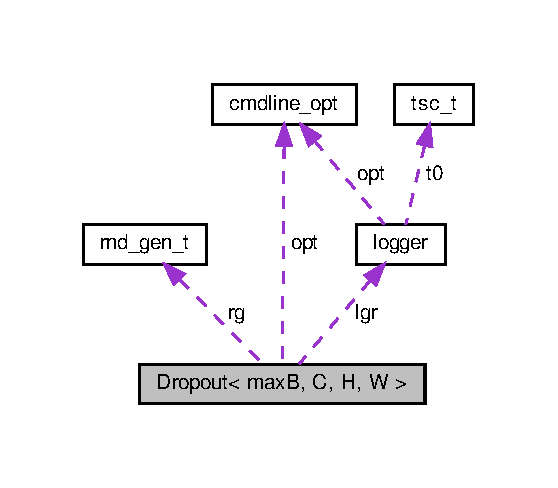
\includegraphics[width=268pt]{structDropout__coll__graph}
\end{center}
\end{figure}
\subsection*{Public Member Functions}
\begin{DoxyCompactItemize}
\item 
void \hyperlink{structDropout_ab684bc3308abad8598f76bdaaa2598ee}{init} (\hyperlink{structcmdline__opt}{cmdline\+\_\+opt} \hyperlink{structDropout_a3d9589e177c7fd00af8d7e82db651e48}{opt}, \hyperlink{structlogger}{logger} $\ast$\hyperlink{structDropout_a55a275be949499a6f3f27fcb9989964e}{lgr}, \hyperlink{vgg__util_8h_a1082d08aaa761215ec83e7149f27ad16}{real} \hyperlink{structDropout_a4181a1bcb986c62b1c6a82a3c1e03d9f}{drop\+\_\+ratio}, long drop\+\_\+seed)
\begin{DoxyCompactList}\small\item\em initialize \end{DoxyCompactList}\item 
\hyperlink{structDropout}{Dropout}$<$ maxB, C, H, W $>$ $\ast$ \hyperlink{structDropout_a364b0df75c98d5b73fd11a77bf11bf89}{copy} ()
\begin{DoxyCompactList}\small\item\em make a copy of this \end{DoxyCompactList}\item 
void \hyperlink{structDropout_aacd2c2da4fb3bd6718b2b43bc26538b9}{set\+\_\+dev} (\hyperlink{structDropout}{Dropout}$<$ maxB, C, H, W $>$ $\ast$\hyperlink{structDropout_a2ce2e6920dfb911f679af91ff9b6de55}{dev})
\begin{DoxyCompactList}\small\item\em set the device pointer for this and all subobjects \end{DoxyCompactList}\item 
void \hyperlink{structDropout_ad1ea86b3d3240a95c9b8c52756ef23a9}{make\+\_\+dev} ()
\begin{DoxyCompactList}\small\item\em if the algorithm is a gpu algorithm, allocate a device shadow of this object and set dev field of this and all subobjects. otherwise it sets all dev fields to null. \end{DoxyCompactList}\item 
void \hyperlink{structDropout_a34adb045be5a2a9546ff99fec3ba1f30}{del\+\_\+dev} ()
\begin{DoxyCompactList}\small\item\em if the algorithm is a gpu algorithm, dev field must not be null and deallocate it. \end{DoxyCompactList}\item 
\mbox{\Hypertarget{structDropout_afbc57376fb281fd9ab79851c9a9af0fa}\label{structDropout_afbc57376fb281fd9ab79851c9a9af0fa}} 
void \hyperlink{structDropout_afbc57376fb281fd9ab79851c9a9af0fa}{to\+\_\+dev} ()
\begin{DoxyCompactList}\small\item\em if the algorithm is a gpu algorithm, dev field must not be null and send the host data to the device memory \end{DoxyCompactList}\item 
\mbox{\Hypertarget{structDropout_a69ab2243eeca5c39bf88540aed92fcdc}\label{structDropout_a69ab2243eeca5c39bf88540aed92fcdc}} 
void \hyperlink{structDropout_a69ab2243eeca5c39bf88540aed92fcdc}{to\+\_\+host} ()
\begin{DoxyCompactList}\small\item\em if the algorithm is a gpu algorithm, dev field must not be null and send the device data to the host memory \end{DoxyCompactList}\item 
\+\_\+\+\_\+device\+\_\+\+\_\+ \+\_\+\+\_\+host\+\_\+\+\_\+ void \hyperlink{structDropout_a8d7db70a48a4c2e3887c931b099f1160}{forward\+\_\+base} (\hyperlink{structarray4}{array4}$<$ maxB, C, H, W $>$ \&x)
\begin{DoxyCompactList}\small\item\em the baseline (serial) implementation of forward called both by cpu implementation (forward\+\_\+cpu) and gpu implementation (forward\+\_\+dev). the call sequence forward -\/$>$ forward\+\_\+cpu -\/$>$ forward\+\_\+base on cpu and and is forward -\/$>$ forward\+\_\+gpu -\/$>$ forward\+\_\+global -\/$>$ forward\+\_\+dev -\/$>$ forward\+\_\+base \end{DoxyCompactList}\item 
\+\_\+\+\_\+device\+\_\+\+\_\+ void \hyperlink{structDropout_a81ee0268c4195380873af8ced5b1acc7}{forward\+\_\+dev} (\hyperlink{structarray4}{array4}$<$ maxB, C, H, W $>$ \&x)
\begin{DoxyCompactList}\small\item\em the device function of forward called from the global (non-\/member) function \end{DoxyCompactList}\item 
void \hyperlink{structDropout_a3bb7569a99e88c36e508bee45f379fad}{forward\+\_\+gpu} (\hyperlink{structarray4}{array4}$<$ maxB, C, H, W $>$ \&x)
\begin{DoxyCompactList}\small\item\em a gpu version of baseline code called from the entry function (forward) \end{DoxyCompactList}\item 
void \hyperlink{structDropout_a2adc263cee9f2d84a8d0729ffaf924a6}{forward\+\_\+cpu} (\hyperlink{structarray4}{array4}$<$ maxB, C, H, W $>$ \&x)
\begin{DoxyCompactList}\small\item\em a cpu version of baseline code called from the entry function (forward) \end{DoxyCompactList}\item 
\hyperlink{structarray4}{array4}$<$ maxB, C, W, H $>$ \& \hyperlink{structDropout_a155eb3ad77df591bdd95645fec1f2089}{forward} (\hyperlink{structarray4}{array4}$<$ maxB, C, H, W $>$ \&x)
\begin{DoxyCompactList}\small\item\em calc the loss function of a mini-\/batch (x) \end{DoxyCompactList}\item 
\+\_\+\+\_\+device\+\_\+\+\_\+ \+\_\+\+\_\+host\+\_\+\+\_\+ void \hyperlink{structDropout_a8ea26e89ddc6b5e4546f5a6ed019ad9a}{backward\+\_\+base} (\hyperlink{structarray4}{array4}$<$ maxB, C, H, W $>$ \&gy)
\begin{DoxyCompactList}\small\item\em the baseline (serial) implementation of backward called both by cpu implementation (backward\+\_\+cpu) and gpu implementation (backward\+\_\+dev). the call sequence backward -\/$>$ backward\+\_\+cpu -\/$>$ backward\+\_\+base on cpu and and is backward -\/$>$ backward\+\_\+gpu -\/$>$ backward\+\_\+global -\/$>$ backward\+\_\+dev -\/$>$ backward\+\_\+base \end{DoxyCompactList}\item 
\+\_\+\+\_\+device\+\_\+\+\_\+ void \hyperlink{structDropout_a5bbc54ad4125bf6768b5eeb17802a468}{backward\+\_\+dev} (\hyperlink{structarray4}{array4}$<$ maxB, C, H, W $>$ \&gy)
\begin{DoxyCompactList}\small\item\em the device function of backward called from the global (non-\/member) function \end{DoxyCompactList}\item 
void \hyperlink{structDropout_a138fbe07114851e478ac794629b6f44a}{backward\+\_\+gpu} (\hyperlink{structarray4}{array4}$<$ maxB, C, H, W $>$ \&gy)
\begin{DoxyCompactList}\small\item\em a gpu version of baseline code called from the entry function (backward) \end{DoxyCompactList}\item 
void \hyperlink{structDropout_a6f78f35970607365a64e5f447bed4c04}{backward\+\_\+cpu} (\hyperlink{structarray4}{array4}$<$ maxB, C, H, W $>$ \&gy)
\begin{DoxyCompactList}\small\item\em a cpu version of baseline code called from the entry function (backward) \end{DoxyCompactList}\item 
\hyperlink{structarray4}{array4}$<$ maxB, C, H, W $>$ \& \hyperlink{structDropout_afe1afe7ce80e59d1b48c820a724aae1b}{backward} (\hyperlink{structarray4}{array4}$<$ maxB, C, H, W $>$ \&gy)
\begin{DoxyCompactList}\small\item\em calc the gradient of loss wrt the input (x) \end{DoxyCompactList}\end{DoxyCompactItemize}
\subsection*{Public Attributes}
\begin{DoxyCompactItemize}
\item 
\hyperlink{structDropout}{Dropout}$<$ maxB, C, H, W $>$ $\ast$ \hyperlink{structDropout_a2ce2e6920dfb911f679af91ff9b6de55}{dev}
\item 
\hyperlink{structcmdline__opt}{cmdline\+\_\+opt} \hyperlink{structDropout_a3d9589e177c7fd00af8d7e82db651e48}{opt}
\item 
\hyperlink{structlogger}{logger} $\ast$ \hyperlink{structDropout_a55a275be949499a6f3f27fcb9989964e}{lgr}
\item 
\hyperlink{structrnd__gen__t}{rnd\+\_\+gen\+\_\+t} \hyperlink{structDropout_a176eb537c9aef161087863244f1e637f}{rg}
\item 
\hyperlink{structarray4}{array4}$<$ maxB, C, H, W $>$ \hyperlink{structDropout_ad758df2bfbd791e6b25e29c8204e0df4}{y}
\item 
\hyperlink{structarray4}{array4}$<$ maxB, C, H, W $>$ \hyperlink{structDropout_a1cf5aced88d251c6b49772ad318bbd27}{gx}
\item 
\hyperlink{vgg__util_8h_a1082d08aaa761215ec83e7149f27ad16}{real} \hyperlink{structDropout_a4181a1bcb986c62b1c6a82a3c1e03d9f}{drop\+\_\+ratio}
\item 
long \hyperlink{structDropout_ac409c1b3a996e35eb78964aa52c5a203}{state\+\_\+forward}
\end{DoxyCompactItemize}


\subsection{Detailed Description}
\subsubsection*{template$<$idx\+\_\+t maxB, idx\+\_\+t C, idx\+\_\+t H, idx\+\_\+t W$>$\newline
struct Dropout$<$ max\+B, C, H, W $>$}

dropout layer 


\begin{DoxyParams}{Parameters}
{\em (max\+B)} & the maximum number of images (batch size) \\
\hline
{\em (\+C)} & the number of channels per input image (the original input has typically three channels for R\+GB. in hidden layers, it starts from 64 and goes up to 512 in the last hidden layer) \\
\hline
{\em (\+H)} & height of an image (32 for an input image, down to 1 in the last hidden layer) \\
\hline
{\em (\+W)} & width of an image (32 for an input image, down to 1 in the last hidden layer)\\
\hline
\end{DoxyParams}
this layer normalizes a batch of images 

\subsection{Member Function Documentation}
\mbox{\Hypertarget{structDropout_afe1afe7ce80e59d1b48c820a724aae1b}\label{structDropout_afe1afe7ce80e59d1b48c820a724aae1b}} 
\index{Dropout@{Dropout}!backward@{backward}}
\index{backward@{backward}!Dropout@{Dropout}}
\subsubsection{\texorpdfstring{backward()}{backward()}}
{\footnotesize\ttfamily template$<$idx\+\_\+t maxB, idx\+\_\+t C, idx\+\_\+t H, idx\+\_\+t W$>$ \\
\hyperlink{structarray4}{array4}$<$maxB,C,H,W$>$\& \hyperlink{structDropout}{Dropout}$<$ maxB, C, H, W $>$\+::backward (\begin{DoxyParamCaption}\item[{\hyperlink{structarray4}{array4}$<$ maxB, C, H, W $>$ \&}]{gy }\end{DoxyParamCaption})\hspace{0.3cm}{\ttfamily [inline]}}



calc the gradient of loss wrt the input (x) 


\begin{DoxyParams}{Parameters}
{\em (gy)} & gradient of loss with respect to the output\\
\hline
\end{DoxyParams}
calc the gradient of loss wrt the input. along the way, it also calculates the gradient of loss wrt weights for all sublayers that have weights. since this is the entire network, gy is actually a vector whose components are all 1. (loss = sum of losses of each data). \begin{DoxySeeAlso}{See also}
\hyperlink{structDropout_a155eb3ad77df591bdd95645fec1f2089}{forward} 

update 
\end{DoxySeeAlso}
\mbox{\Hypertarget{structDropout_a8ea26e89ddc6b5e4546f5a6ed019ad9a}\label{structDropout_a8ea26e89ddc6b5e4546f5a6ed019ad9a}} 
\index{Dropout@{Dropout}!backward\+\_\+base@{backward\+\_\+base}}
\index{backward\+\_\+base@{backward\+\_\+base}!Dropout@{Dropout}}
\subsubsection{\texorpdfstring{backward\+\_\+base()}{backward\_base()}}
{\footnotesize\ttfamily template$<$idx\+\_\+t maxB, idx\+\_\+t C, idx\+\_\+t H, idx\+\_\+t W$>$ \\
\+\_\+\+\_\+device\+\_\+\+\_\+ \+\_\+\+\_\+host\+\_\+\+\_\+ void \hyperlink{structDropout}{Dropout}$<$ maxB, C, H, W $>$\+::backward\+\_\+base (\begin{DoxyParamCaption}\item[{\hyperlink{structarray4}{array4}$<$ maxB, C, H, W $>$ \&}]{gy }\end{DoxyParamCaption})\hspace{0.3cm}{\ttfamily [inline]}}



the baseline (serial) implementation of backward called both by cpu implementation (backward\+\_\+cpu) and gpu implementation (backward\+\_\+dev). the call sequence backward -\/$>$ backward\+\_\+cpu -\/$>$ backward\+\_\+base on cpu and and is backward -\/$>$ backward\+\_\+gpu -\/$>$ backward\+\_\+global -\/$>$ backward\+\_\+dev -\/$>$ backward\+\_\+base 


\begin{DoxyParams}{Parameters}
{\em (gy)} & gradient of loss with respect to the output \\
\hline
\end{DoxyParams}
\begin{DoxySeeAlso}{See also}
\hyperlink{structDropout_afe1afe7ce80e59d1b48c820a724aae1b}{backward} 

\hyperlink{structDropout_a138fbe07114851e478ac794629b6f44a}{backward\+\_\+gpu} 

\hyperlink{softmaxcrossentropy_8h_a47d56a9a23e08247b227f4aac17413e0}{backward\+\_\+global} 

\hyperlink{structDropout_a5bbc54ad4125bf6768b5eeb17802a468}{backward\+\_\+dev} 
\end{DoxySeeAlso}
\mbox{\Hypertarget{structDropout_a6f78f35970607365a64e5f447bed4c04}\label{structDropout_a6f78f35970607365a64e5f447bed4c04}} 
\index{Dropout@{Dropout}!backward\+\_\+cpu@{backward\+\_\+cpu}}
\index{backward\+\_\+cpu@{backward\+\_\+cpu}!Dropout@{Dropout}}
\subsubsection{\texorpdfstring{backward\+\_\+cpu()}{backward\_cpu()}}
{\footnotesize\ttfamily template$<$idx\+\_\+t maxB, idx\+\_\+t C, idx\+\_\+t H, idx\+\_\+t W$>$ \\
void \hyperlink{structDropout}{Dropout}$<$ maxB, C, H, W $>$\+::backward\+\_\+cpu (\begin{DoxyParamCaption}\item[{\hyperlink{structarray4}{array4}$<$ maxB, C, H, W $>$ \&}]{gy }\end{DoxyParamCaption})\hspace{0.3cm}{\ttfamily [inline]}}



a cpu version of baseline code called from the entry function (backward) 


\begin{DoxyParams}{Parameters}
{\em (gy)} & gradient of loss with respect to the output \\
\hline
\end{DoxyParams}
\begin{DoxySeeAlso}{See also}
\hyperlink{structDropout_afe1afe7ce80e59d1b48c820a724aae1b}{backward} 

\hyperlink{structDropout_a8ea26e89ddc6b5e4546f5a6ed019ad9a}{backward\+\_\+base} 
\end{DoxySeeAlso}
\mbox{\Hypertarget{structDropout_a5bbc54ad4125bf6768b5eeb17802a468}\label{structDropout_a5bbc54ad4125bf6768b5eeb17802a468}} 
\index{Dropout@{Dropout}!backward\+\_\+dev@{backward\+\_\+dev}}
\index{backward\+\_\+dev@{backward\+\_\+dev}!Dropout@{Dropout}}
\subsubsection{\texorpdfstring{backward\+\_\+dev()}{backward\_dev()}}
{\footnotesize\ttfamily template$<$idx\+\_\+t maxB, idx\+\_\+t C, idx\+\_\+t H, idx\+\_\+t W$>$ \\
\+\_\+\+\_\+device\+\_\+\+\_\+ void \hyperlink{structDropout}{Dropout}$<$ maxB, C, H, W $>$\+::backward\+\_\+dev (\begin{DoxyParamCaption}\item[{\hyperlink{structarray4}{array4}$<$ maxB, C, H, W $>$ \&}]{gy }\end{DoxyParamCaption})\hspace{0.3cm}{\ttfamily [inline]}}



the device function of backward called from the global (non-\/member) function 


\begin{DoxyParams}{Parameters}
{\em (gy)} & gradient of loss with respect to the output \\
\hline
\end{DoxyParams}
\begin{DoxySeeAlso}{See also}
\hyperlink{structDropout_afe1afe7ce80e59d1b48c820a724aae1b}{backward} 

\hyperlink{structDropout_a138fbe07114851e478ac794629b6f44a}{backward\+\_\+gpu} 

\hyperlink{softmaxcrossentropy_8h_a47d56a9a23e08247b227f4aac17413e0}{backward\+\_\+global} 

\hyperlink{structDropout_a8ea26e89ddc6b5e4546f5a6ed019ad9a}{backward\+\_\+base} 
\end{DoxySeeAlso}
\mbox{\Hypertarget{structDropout_a138fbe07114851e478ac794629b6f44a}\label{structDropout_a138fbe07114851e478ac794629b6f44a}} 
\index{Dropout@{Dropout}!backward\+\_\+gpu@{backward\+\_\+gpu}}
\index{backward\+\_\+gpu@{backward\+\_\+gpu}!Dropout@{Dropout}}
\subsubsection{\texorpdfstring{backward\+\_\+gpu()}{backward\_gpu()}}
{\footnotesize\ttfamily template$<$idx\+\_\+t maxB, idx\+\_\+t C, idx\+\_\+t H, idx\+\_\+t W$>$ \\
void \hyperlink{structDropout}{Dropout}$<$ maxB, C, H, W $>$\+::backward\+\_\+gpu (\begin{DoxyParamCaption}\item[{\hyperlink{structarray4}{array4}$<$ maxB, C, H, W $>$ \&}]{gy }\end{DoxyParamCaption})\hspace{0.3cm}{\ttfamily [inline]}}



a gpu version of baseline code called from the entry function (backward) 


\begin{DoxyParams}{Parameters}
{\em (gy)} & gradient of loss with respect to the output \\
\hline
\end{DoxyParams}
\begin{DoxySeeAlso}{See also}
\hyperlink{structDropout_afe1afe7ce80e59d1b48c820a724aae1b}{backward} 

\hyperlink{softmaxcrossentropy_8h_a47d56a9a23e08247b227f4aac17413e0}{backward\+\_\+global} 

\hyperlink{structDropout_a5bbc54ad4125bf6768b5eeb17802a468}{backward\+\_\+dev} 

\hyperlink{structDropout_a8ea26e89ddc6b5e4546f5a6ed019ad9a}{backward\+\_\+base} 
\end{DoxySeeAlso}
\mbox{\Hypertarget{structDropout_a364b0df75c98d5b73fd11a77bf11bf89}\label{structDropout_a364b0df75c98d5b73fd11a77bf11bf89}} 
\index{Dropout@{Dropout}!copy@{copy}}
\index{copy@{copy}!Dropout@{Dropout}}
\subsubsection{\texorpdfstring{copy()}{copy()}}
{\footnotesize\ttfamily template$<$idx\+\_\+t maxB, idx\+\_\+t C, idx\+\_\+t H, idx\+\_\+t W$>$ \\
\hyperlink{structDropout}{Dropout}$<$maxB,C,H,W$>$$\ast$ \hyperlink{structDropout}{Dropout}$<$ maxB, C, H, W $>$\+::copy (\begin{DoxyParamCaption}{ }\end{DoxyParamCaption})\hspace{0.3cm}{\ttfamily [inline]}}



make a copy of this 

if this object has a device pointer, the copy will have a device pointer too, but its contents are N\+OT copied \mbox{\Hypertarget{structDropout_a34adb045be5a2a9546ff99fec3ba1f30}\label{structDropout_a34adb045be5a2a9546ff99fec3ba1f30}} 
\index{Dropout@{Dropout}!del\+\_\+dev@{del\+\_\+dev}}
\index{del\+\_\+dev@{del\+\_\+dev}!Dropout@{Dropout}}
\subsubsection{\texorpdfstring{del\+\_\+dev()}{del\_dev()}}
{\footnotesize\ttfamily template$<$idx\+\_\+t maxB, idx\+\_\+t C, idx\+\_\+t H, idx\+\_\+t W$>$ \\
void \hyperlink{structDropout}{Dropout}$<$ maxB, C, H, W $>$\+::del\+\_\+dev (\begin{DoxyParamCaption}{ }\end{DoxyParamCaption})\hspace{0.3cm}{\ttfamily [inline]}}



if the algorithm is a gpu algorithm, dev field must not be null and deallocate it. 

\begin{DoxySeeAlso}{See also}
\hyperlink{structDropout_ad1ea86b3d3240a95c9b8c52756ef23a9}{make\+\_\+dev} 

\hyperlink{structDropout_aacd2c2da4fb3bd6718b2b43bc26538b9}{set\+\_\+dev} 
\end{DoxySeeAlso}
\mbox{\Hypertarget{structDropout_a155eb3ad77df591bdd95645fec1f2089}\label{structDropout_a155eb3ad77df591bdd95645fec1f2089}} 
\index{Dropout@{Dropout}!forward@{forward}}
\index{forward@{forward}!Dropout@{Dropout}}
\subsubsection{\texorpdfstring{forward()}{forward()}}
{\footnotesize\ttfamily template$<$idx\+\_\+t maxB, idx\+\_\+t C, idx\+\_\+t H, idx\+\_\+t W$>$ \\
\hyperlink{structarray4}{array4}$<$maxB,C,W,H$>$\& \hyperlink{structDropout}{Dropout}$<$ maxB, C, H, W $>$\+::forward (\begin{DoxyParamCaption}\item[{\hyperlink{structarray4}{array4}$<$ maxB, C, H, W $>$ \&}]{x }\end{DoxyParamCaption})\hspace{0.3cm}{\ttfamily [inline]}}



calc the loss function of a mini-\/batch (x) 


\begin{DoxyParams}{Parameters}
{\em (x)} & input images \\
\hline
\end{DoxyParams}
\begin{DoxySeeAlso}{See also}
\hyperlink{structDropout_afe1afe7ce80e59d1b48c820a724aae1b}{backward} 

update 
\end{DoxySeeAlso}
\mbox{\Hypertarget{structDropout_a8d7db70a48a4c2e3887c931b099f1160}\label{structDropout_a8d7db70a48a4c2e3887c931b099f1160}} 
\index{Dropout@{Dropout}!forward\+\_\+base@{forward\+\_\+base}}
\index{forward\+\_\+base@{forward\+\_\+base}!Dropout@{Dropout}}
\subsubsection{\texorpdfstring{forward\+\_\+base()}{forward\_base()}}
{\footnotesize\ttfamily template$<$idx\+\_\+t maxB, idx\+\_\+t C, idx\+\_\+t H, idx\+\_\+t W$>$ \\
\+\_\+\+\_\+device\+\_\+\+\_\+ \+\_\+\+\_\+host\+\_\+\+\_\+ void \hyperlink{structDropout}{Dropout}$<$ maxB, C, H, W $>$\+::forward\+\_\+base (\begin{DoxyParamCaption}\item[{\hyperlink{structarray4}{array4}$<$ maxB, C, H, W $>$ \&}]{x }\end{DoxyParamCaption})\hspace{0.3cm}{\ttfamily [inline]}}



the baseline (serial) implementation of forward called both by cpu implementation (forward\+\_\+cpu) and gpu implementation (forward\+\_\+dev). the call sequence forward -\/$>$ forward\+\_\+cpu -\/$>$ forward\+\_\+base on cpu and and is forward -\/$>$ forward\+\_\+gpu -\/$>$ forward\+\_\+global -\/$>$ forward\+\_\+dev -\/$>$ forward\+\_\+base 


\begin{DoxyParams}{Parameters}
{\em (x)} & input images \\
\hline
\end{DoxyParams}
\begin{DoxySeeAlso}{See also}
\hyperlink{structDropout_a155eb3ad77df591bdd95645fec1f2089}{forward} 

\hyperlink{structDropout_a3bb7569a99e88c36e508bee45f379fad}{forward\+\_\+gpu} 

\hyperlink{softmaxcrossentropy_8h_a578aeeb166bd06e800d9b396eab48b35}{forward\+\_\+global} 

\hyperlink{structDropout_a81ee0268c4195380873af8ced5b1acc7}{forward\+\_\+dev} 
\end{DoxySeeAlso}
\mbox{\Hypertarget{structDropout_a2adc263cee9f2d84a8d0729ffaf924a6}\label{structDropout_a2adc263cee9f2d84a8d0729ffaf924a6}} 
\index{Dropout@{Dropout}!forward\+\_\+cpu@{forward\+\_\+cpu}}
\index{forward\+\_\+cpu@{forward\+\_\+cpu}!Dropout@{Dropout}}
\subsubsection{\texorpdfstring{forward\+\_\+cpu()}{forward\_cpu()}}
{\footnotesize\ttfamily template$<$idx\+\_\+t maxB, idx\+\_\+t C, idx\+\_\+t H, idx\+\_\+t W$>$ \\
void \hyperlink{structDropout}{Dropout}$<$ maxB, C, H, W $>$\+::forward\+\_\+cpu (\begin{DoxyParamCaption}\item[{\hyperlink{structarray4}{array4}$<$ maxB, C, H, W $>$ \&}]{x }\end{DoxyParamCaption})\hspace{0.3cm}{\ttfamily [inline]}}



a cpu version of baseline code called from the entry function (forward) 


\begin{DoxyParams}{Parameters}
{\em (x)} & input images \\
\hline
\end{DoxyParams}
\begin{DoxySeeAlso}{See also}
\hyperlink{structDropout_a155eb3ad77df591bdd95645fec1f2089}{forward} 

\hyperlink{structDropout_a8d7db70a48a4c2e3887c931b099f1160}{forward\+\_\+base} 
\end{DoxySeeAlso}
\mbox{\Hypertarget{structDropout_a81ee0268c4195380873af8ced5b1acc7}\label{structDropout_a81ee0268c4195380873af8ced5b1acc7}} 
\index{Dropout@{Dropout}!forward\+\_\+dev@{forward\+\_\+dev}}
\index{forward\+\_\+dev@{forward\+\_\+dev}!Dropout@{Dropout}}
\subsubsection{\texorpdfstring{forward\+\_\+dev()}{forward\_dev()}}
{\footnotesize\ttfamily template$<$idx\+\_\+t maxB, idx\+\_\+t C, idx\+\_\+t H, idx\+\_\+t W$>$ \\
\+\_\+\+\_\+device\+\_\+\+\_\+ void \hyperlink{structDropout}{Dropout}$<$ maxB, C, H, W $>$\+::forward\+\_\+dev (\begin{DoxyParamCaption}\item[{\hyperlink{structarray4}{array4}$<$ maxB, C, H, W $>$ \&}]{x }\end{DoxyParamCaption})\hspace{0.3cm}{\ttfamily [inline]}}



the device function of forward called from the global (non-\/member) function 


\begin{DoxyParams}{Parameters}
{\em (x)} & input images \\
\hline
\end{DoxyParams}
\begin{DoxySeeAlso}{See also}
\hyperlink{structDropout_a155eb3ad77df591bdd95645fec1f2089}{forward} 

\hyperlink{structDropout_a3bb7569a99e88c36e508bee45f379fad}{forward\+\_\+gpu} 

\hyperlink{softmaxcrossentropy_8h_a578aeeb166bd06e800d9b396eab48b35}{forward\+\_\+global} 

\hyperlink{structDropout_a8d7db70a48a4c2e3887c931b099f1160}{forward\+\_\+base} 
\end{DoxySeeAlso}
\mbox{\Hypertarget{structDropout_a3bb7569a99e88c36e508bee45f379fad}\label{structDropout_a3bb7569a99e88c36e508bee45f379fad}} 
\index{Dropout@{Dropout}!forward\+\_\+gpu@{forward\+\_\+gpu}}
\index{forward\+\_\+gpu@{forward\+\_\+gpu}!Dropout@{Dropout}}
\subsubsection{\texorpdfstring{forward\+\_\+gpu()}{forward\_gpu()}}
{\footnotesize\ttfamily template$<$idx\+\_\+t maxB, idx\+\_\+t C, idx\+\_\+t H, idx\+\_\+t W$>$ \\
void \hyperlink{structDropout}{Dropout}$<$ maxB, C, H, W $>$\+::forward\+\_\+gpu (\begin{DoxyParamCaption}\item[{\hyperlink{structarray4}{array4}$<$ maxB, C, H, W $>$ \&}]{x }\end{DoxyParamCaption})\hspace{0.3cm}{\ttfamily [inline]}}



a gpu version of baseline code called from the entry function (forward) 


\begin{DoxyParams}{Parameters}
{\em (x)} & input images \\
\hline
\end{DoxyParams}
\begin{DoxySeeAlso}{See also}
\hyperlink{structDropout_a155eb3ad77df591bdd95645fec1f2089}{forward} 

\hyperlink{softmaxcrossentropy_8h_a578aeeb166bd06e800d9b396eab48b35}{forward\+\_\+global} 

\hyperlink{structDropout_a81ee0268c4195380873af8ced5b1acc7}{forward\+\_\+dev} 

\hyperlink{structDropout_a8d7db70a48a4c2e3887c931b099f1160}{forward\+\_\+base} 
\end{DoxySeeAlso}
\mbox{\Hypertarget{structDropout_ab684bc3308abad8598f76bdaaa2598ee}\label{structDropout_ab684bc3308abad8598f76bdaaa2598ee}} 
\index{Dropout@{Dropout}!init@{init}}
\index{init@{init}!Dropout@{Dropout}}
\subsubsection{\texorpdfstring{init()}{init()}}
{\footnotesize\ttfamily template$<$idx\+\_\+t maxB, idx\+\_\+t C, idx\+\_\+t H, idx\+\_\+t W$>$ \\
void \hyperlink{structDropout}{Dropout}$<$ maxB, C, H, W $>$\+::init (\begin{DoxyParamCaption}\item[{\hyperlink{structcmdline__opt}{cmdline\+\_\+opt}}]{opt,  }\item[{\hyperlink{structlogger}{logger} $\ast$}]{lgr,  }\item[{\hyperlink{vgg__util_8h_a1082d08aaa761215ec83e7149f27ad16}{real}}]{drop\+\_\+ratio,  }\item[{long}]{drop\+\_\+seed }\end{DoxyParamCaption})\hspace{0.3cm}{\ttfamily [inline]}}



initialize 


\begin{DoxyParams}{Parameters}
{\em (opt)} & command line options \\
\hline
{\em (lgr)} & logger \\
\hline
{\em (drop\+\_\+ratio)} & the probability each cell is dropped out \\
\hline
{\em (drop\+\_\+seed)} & the seed of the random number generator used to determine dropout \\
\hline
\end{DoxyParams}
\mbox{\Hypertarget{structDropout_ad1ea86b3d3240a95c9b8c52756ef23a9}\label{structDropout_ad1ea86b3d3240a95c9b8c52756ef23a9}} 
\index{Dropout@{Dropout}!make\+\_\+dev@{make\+\_\+dev}}
\index{make\+\_\+dev@{make\+\_\+dev}!Dropout@{Dropout}}
\subsubsection{\texorpdfstring{make\+\_\+dev()}{make\_dev()}}
{\footnotesize\ttfamily template$<$idx\+\_\+t maxB, idx\+\_\+t C, idx\+\_\+t H, idx\+\_\+t W$>$ \\
void \hyperlink{structDropout}{Dropout}$<$ maxB, C, H, W $>$\+::make\+\_\+dev (\begin{DoxyParamCaption}{ }\end{DoxyParamCaption})\hspace{0.3cm}{\ttfamily [inline]}}



if the algorithm is a gpu algorithm, allocate a device shadow of this object and set dev field of this and all subobjects. otherwise it sets all dev fields to null. 

\begin{DoxySeeAlso}{See also}
\hyperlink{structDropout_aacd2c2da4fb3bd6718b2b43bc26538b9}{set\+\_\+dev} 

\hyperlink{structDropout_a34adb045be5a2a9546ff99fec3ba1f30}{del\+\_\+dev} 
\end{DoxySeeAlso}
\mbox{\Hypertarget{structDropout_aacd2c2da4fb3bd6718b2b43bc26538b9}\label{structDropout_aacd2c2da4fb3bd6718b2b43bc26538b9}} 
\index{Dropout@{Dropout}!set\+\_\+dev@{set\+\_\+dev}}
\index{set\+\_\+dev@{set\+\_\+dev}!Dropout@{Dropout}}
\subsubsection{\texorpdfstring{set\+\_\+dev()}{set\_dev()}}
{\footnotesize\ttfamily template$<$idx\+\_\+t maxB, idx\+\_\+t C, idx\+\_\+t H, idx\+\_\+t W$>$ \\
void \hyperlink{structDropout}{Dropout}$<$ maxB, C, H, W $>$\+::set\+\_\+dev (\begin{DoxyParamCaption}\item[{\hyperlink{structDropout}{Dropout}$<$ maxB, C, H, W $>$ $\ast$}]{dev }\end{DoxyParamCaption})\hspace{0.3cm}{\ttfamily [inline]}}



set the device pointer for this and all subobjects 


\begin{DoxyParams}{Parameters}
{\em (dev)} & a device memory or null \\
\hline
\end{DoxyParams}
\begin{DoxySeeAlso}{See also}
\hyperlink{structDropout_ad1ea86b3d3240a95c9b8c52756ef23a9}{make\+\_\+dev} 

\hyperlink{structDropout_a34adb045be5a2a9546ff99fec3ba1f30}{del\+\_\+dev}
\end{DoxySeeAlso}
if dev is not null, dev fields of all subojects point to the corresponding subjects in the device memory. if dev is not null, all dev fields become null. 

\subsection{Member Data Documentation}
\mbox{\Hypertarget{structDropout_a2ce2e6920dfb911f679af91ff9b6de55}\label{structDropout_a2ce2e6920dfb911f679af91ff9b6de55}} 
\index{Dropout@{Dropout}!dev@{dev}}
\index{dev@{dev}!Dropout@{Dropout}}
\subsubsection{\texorpdfstring{dev}{dev}}
{\footnotesize\ttfamily template$<$idx\+\_\+t maxB, idx\+\_\+t C, idx\+\_\+t H, idx\+\_\+t W$>$ \\
\hyperlink{structDropout}{Dropout}$<$maxB,C,H,W$>$$\ast$ \hyperlink{structDropout}{Dropout}$<$ maxB, C, H, W $>$\+::dev}

device shadow \mbox{\Hypertarget{structDropout_a4181a1bcb986c62b1c6a82a3c1e03d9f}\label{structDropout_a4181a1bcb986c62b1c6a82a3c1e03d9f}} 
\index{Dropout@{Dropout}!drop\+\_\+ratio@{drop\+\_\+ratio}}
\index{drop\+\_\+ratio@{drop\+\_\+ratio}!Dropout@{Dropout}}
\subsubsection{\texorpdfstring{drop\+\_\+ratio}{drop\_ratio}}
{\footnotesize\ttfamily template$<$idx\+\_\+t maxB, idx\+\_\+t C, idx\+\_\+t H, idx\+\_\+t W$>$ \\
\hyperlink{vgg__util_8h_a1082d08aaa761215ec83e7149f27ad16}{real} \hyperlink{structDropout}{Dropout}$<$ maxB, C, H, W $>$\+::drop\+\_\+ratio}

drop probability \mbox{\Hypertarget{structDropout_a1cf5aced88d251c6b49772ad318bbd27}\label{structDropout_a1cf5aced88d251c6b49772ad318bbd27}} 
\index{Dropout@{Dropout}!gx@{gx}}
\index{gx@{gx}!Dropout@{Dropout}}
\subsubsection{\texorpdfstring{gx}{gx}}
{\footnotesize\ttfamily template$<$idx\+\_\+t maxB, idx\+\_\+t C, idx\+\_\+t H, idx\+\_\+t W$>$ \\
\hyperlink{structarray4}{array4}$<$maxB,C,H,W$>$ \hyperlink{structDropout}{Dropout}$<$ maxB, C, H, W $>$\+::gx}

gradient of loss wrt to input x \mbox{\Hypertarget{structDropout_a55a275be949499a6f3f27fcb9989964e}\label{structDropout_a55a275be949499a6f3f27fcb9989964e}} 
\index{Dropout@{Dropout}!lgr@{lgr}}
\index{lgr@{lgr}!Dropout@{Dropout}}
\subsubsection{\texorpdfstring{lgr}{lgr}}
{\footnotesize\ttfamily template$<$idx\+\_\+t maxB, idx\+\_\+t C, idx\+\_\+t H, idx\+\_\+t W$>$ \\
\hyperlink{structlogger}{logger}$\ast$ \hyperlink{structDropout}{Dropout}$<$ maxB, C, H, W $>$\+::lgr}

logger \mbox{\Hypertarget{structDropout_a3d9589e177c7fd00af8d7e82db651e48}\label{structDropout_a3d9589e177c7fd00af8d7e82db651e48}} 
\index{Dropout@{Dropout}!opt@{opt}}
\index{opt@{opt}!Dropout@{Dropout}}
\subsubsection{\texorpdfstring{opt}{opt}}
{\footnotesize\ttfamily template$<$idx\+\_\+t maxB, idx\+\_\+t C, idx\+\_\+t H, idx\+\_\+t W$>$ \\
\hyperlink{structcmdline__opt}{cmdline\+\_\+opt} \hyperlink{structDropout}{Dropout}$<$ maxB, C, H, W $>$\+::opt}

command line option \mbox{\Hypertarget{structDropout_a176eb537c9aef161087863244f1e637f}\label{structDropout_a176eb537c9aef161087863244f1e637f}} 
\index{Dropout@{Dropout}!rg@{rg}}
\index{rg@{rg}!Dropout@{Dropout}}
\subsubsection{\texorpdfstring{rg}{rg}}
{\footnotesize\ttfamily template$<$idx\+\_\+t maxB, idx\+\_\+t C, idx\+\_\+t H, idx\+\_\+t W$>$ \\
\hyperlink{structrnd__gen__t}{rnd\+\_\+gen\+\_\+t} \hyperlink{structDropout}{Dropout}$<$ maxB, C, H, W $>$\+::rg}

random number generator to choose dropout \mbox{\Hypertarget{structDropout_ac409c1b3a996e35eb78964aa52c5a203}\label{structDropout_ac409c1b3a996e35eb78964aa52c5a203}} 
\index{Dropout@{Dropout}!state\+\_\+forward@{state\+\_\+forward}}
\index{state\+\_\+forward@{state\+\_\+forward}!Dropout@{Dropout}}
\subsubsection{\texorpdfstring{state\+\_\+forward}{state\_forward}}
{\footnotesize\ttfamily template$<$idx\+\_\+t maxB, idx\+\_\+t C, idx\+\_\+t H, idx\+\_\+t W$>$ \\
long \hyperlink{structDropout}{Dropout}$<$ maxB, C, H, W $>$\+::state\+\_\+forward}

random number state at the forward function \mbox{\Hypertarget{structDropout_ad758df2bfbd791e6b25e29c8204e0df4}\label{structDropout_ad758df2bfbd791e6b25e29c8204e0df4}} 
\index{Dropout@{Dropout}!y@{y}}
\index{y@{y}!Dropout@{Dropout}}
\subsubsection{\texorpdfstring{y}{y}}
{\footnotesize\ttfamily template$<$idx\+\_\+t maxB, idx\+\_\+t C, idx\+\_\+t H, idx\+\_\+t W$>$ \\
\hyperlink{structarray4}{array4}$<$maxB,C,H,W$>$ \hyperlink{structDropout}{Dropout}$<$ maxB, C, H, W $>$\+::y}

output of the forward 

The documentation for this struct was generated from the following file\+:\begin{DoxyCompactItemize}
\item 
/home/tau/public\+\_\+html/lecture/parallel\+\_\+distributed/2018/handson/tau/parallel-\/distributed-\/handson/20vgg/include/\hyperlink{dropout_8h}{dropout.\+h}\end{DoxyCompactItemize}

\hypertarget{structivec}{}\section{ivec$<$ N $>$ Struct Template Reference}
\label{structivec}\index{ivec$<$ N $>$@{ivec$<$ N $>$}}


integer vector  




{\ttfamily \#include $<$vgg\+\_\+arrays.\+h$>$}

\subsection*{Public Member Functions}
\begin{DoxyCompactItemize}
\item 
\+\_\+\+\_\+device\+\_\+\+\_\+ \+\_\+\+\_\+host\+\_\+\+\_\+ \hyperlink{vgg__util_8h_a8e93478a00e685bea5e6a3f617bf03a3}{idx\+\_\+t} \& \hyperlink{structivec_a54625e9b81da8a7aa7756e84a5f79e6f}{operator()} (\hyperlink{vgg__util_8h_a8e93478a00e685bea5e6a3f617bf03a3}{idx\+\_\+t} i)
\begin{DoxyCompactList}\small\item\em access the i-\/th element \end{DoxyCompactList}\item 
\+\_\+\+\_\+device\+\_\+\+\_\+ \+\_\+\+\_\+host\+\_\+\+\_\+ void \hyperlink{structivec_a7bbd67af13e22712f34a954e45f7ab81}{set\+\_\+n} (\hyperlink{vgg__util_8h_a8e93478a00e685bea5e6a3f617bf03a3}{idx\+\_\+t} \hyperlink{structivec_ad067032ec2cffe11fddfa932aa2380d1}{n})
\begin{DoxyCompactList}\small\item\em set the number of elements \end{DoxyCompactList}\item 
void \hyperlink{structivec_a1bf61db14d42b86afa9e0823fd351624}{init\+\_\+const} (\hyperlink{vgg__util_8h_a8e93478a00e685bea5e6a3f617bf03a3}{idx\+\_\+t} \hyperlink{structivec_ad067032ec2cffe11fddfa932aa2380d1}{n}, \hyperlink{vgg__util_8h_a8e93478a00e685bea5e6a3f617bf03a3}{idx\+\_\+t} c)
\begin{DoxyCompactList}\small\item\em initialize elements of the vector to a single constant value \end{DoxyCompactList}\item 
void \hyperlink{structivec_ad2dda0297da5553e346c97cad62fd23e}{init\+\_\+uniform} (\hyperlink{vgg__util_8h_a8e93478a00e685bea5e6a3f617bf03a3}{idx\+\_\+t} \hyperlink{structivec_ad067032ec2cffe11fddfa932aa2380d1}{n}, \hyperlink{structrnd__gen__t}{rnd\+\_\+gen\+\_\+t} \&rg, \hyperlink{vgg__util_8h_a8e93478a00e685bea5e6a3f617bf03a3}{idx\+\_\+t} p, \hyperlink{vgg__util_8h_a8e93478a00e685bea5e6a3f617bf03a3}{idx\+\_\+t} q)
\begin{DoxyCompactList}\small\item\em randomly initialize elements of the vector uniformly between p and q \end{DoxyCompactList}\item 
void \hyperlink{structivec_abe2b4ca3bb19444a5a915676aa333008}{set\+\_\+dev} (\hyperlink{structivec}{ivec}$<$ N $>$ $\ast$\hyperlink{structivec_ac50ca2c5bec8b1fd9e84fb8cba681ed6}{dev})
\begin{DoxyCompactList}\small\item\em set the device shadow of this vector \end{DoxyCompactList}\item 
void \hyperlink{structivec_a70cade2ab506db00fa0df8a66092e646}{make\+\_\+dev} (int gpu)
\begin{DoxyCompactList}\small\item\em allocate and set the device shadow of this vector if requested by the parameter \end{DoxyCompactList}\item 
\mbox{\Hypertarget{structivec_a1ec4ea7f160e1583c777e4a6d31bd128}\label{structivec_a1ec4ea7f160e1583c777e4a6d31bd128}} 
void \hyperlink{structivec_a1ec4ea7f160e1583c777e4a6d31bd128}{del\+\_\+dev} ()
\begin{DoxyCompactList}\small\item\em deallocate the device shadow of this vector \end{DoxyCompactList}\item 
\mbox{\Hypertarget{structivec_a8ba432f4fde0ff661de285625fca5719}\label{structivec_a8ba432f4fde0ff661de285625fca5719}} 
void \hyperlink{structivec_a8ba432f4fde0ff661de285625fca5719}{to\+\_\+dev} ()
\begin{DoxyCompactList}\small\item\em send the data to its gpu shadow \end{DoxyCompactList}\item 
\mbox{\Hypertarget{structivec_a6cbc9444fd57cb38373ac6ba8e7d4e87}\label{structivec_a6cbc9444fd57cb38373ac6ba8e7d4e87}} 
void \hyperlink{structivec_a6cbc9444fd57cb38373ac6ba8e7d4e87}{to\+\_\+host} ()
\begin{DoxyCompactList}\small\item\em get the data back from gpu shadow to host \end{DoxyCompactList}\end{DoxyCompactItemize}
\subsection*{Public Attributes}
\begin{DoxyCompactItemize}
\item 
\hyperlink{structivec}{ivec}$<$ N $>$ $\ast$ \hyperlink{structivec_ac50ca2c5bec8b1fd9e84fb8cba681ed6}{dev}
\item 
\hyperlink{vgg__util_8h_a8e93478a00e685bea5e6a3f617bf03a3}{idx\+\_\+t} \hyperlink{structivec_ad067032ec2cffe11fddfa932aa2380d1}{n}
\item 
\hyperlink{vgg__util_8h_a8e93478a00e685bea5e6a3f617bf03a3}{idx\+\_\+t} \hyperlink{structivec_a8abb4460bee21f081dda79fce44f0dfc}{w} \mbox{[}N\mbox{]}
\end{DoxyCompactItemize}


\subsection{Detailed Description}
\subsubsection*{template$<$idx\+\_\+t N$>$\newline
struct ivec$<$ N $>$}

integer vector 


\begin{DoxyParams}{Parameters}
{\em (\+N)} & the maximun number of elements it can hold \\
\hline
\end{DoxyParams}


\subsection{Member Function Documentation}
\mbox{\Hypertarget{structivec_a1bf61db14d42b86afa9e0823fd351624}\label{structivec_a1bf61db14d42b86afa9e0823fd351624}} 
\index{ivec@{ivec}!init\+\_\+const@{init\+\_\+const}}
\index{init\+\_\+const@{init\+\_\+const}!ivec@{ivec}}
\subsubsection{\texorpdfstring{init\+\_\+const()}{init\_const()}}
{\footnotesize\ttfamily template$<$idx\+\_\+t N$>$ \\
void \hyperlink{structivec}{ivec}$<$ N $>$\+::init\+\_\+const (\begin{DoxyParamCaption}\item[{\hyperlink{vgg__util_8h_a8e93478a00e685bea5e6a3f617bf03a3}{idx\+\_\+t}}]{n,  }\item[{\hyperlink{vgg__util_8h_a8e93478a00e685bea5e6a3f617bf03a3}{idx\+\_\+t}}]{c }\end{DoxyParamCaption})\hspace{0.3cm}{\ttfamily [inline]}}



initialize elements of the vector to a single constant value 


\begin{DoxyParams}{Parameters}
{\em (n)} & the number of elements to initialize \\
\hline
{\em (c)} & the value of each element \\
\hline
\end{DoxyParams}
\mbox{\Hypertarget{structivec_ad2dda0297da5553e346c97cad62fd23e}\label{structivec_ad2dda0297da5553e346c97cad62fd23e}} 
\index{ivec@{ivec}!init\+\_\+uniform@{init\+\_\+uniform}}
\index{init\+\_\+uniform@{init\+\_\+uniform}!ivec@{ivec}}
\subsubsection{\texorpdfstring{init\+\_\+uniform()}{init\_uniform()}}
{\footnotesize\ttfamily template$<$idx\+\_\+t N$>$ \\
void \hyperlink{structivec}{ivec}$<$ N $>$\+::init\+\_\+uniform (\begin{DoxyParamCaption}\item[{\hyperlink{vgg__util_8h_a8e93478a00e685bea5e6a3f617bf03a3}{idx\+\_\+t}}]{n,  }\item[{\hyperlink{structrnd__gen__t}{rnd\+\_\+gen\+\_\+t} \&}]{rg,  }\item[{\hyperlink{vgg__util_8h_a8e93478a00e685bea5e6a3f617bf03a3}{idx\+\_\+t}}]{p,  }\item[{\hyperlink{vgg__util_8h_a8e93478a00e685bea5e6a3f617bf03a3}{idx\+\_\+t}}]{q }\end{DoxyParamCaption})\hspace{0.3cm}{\ttfamily [inline]}}



randomly initialize elements of the vector uniformly between p and q 


\begin{DoxyParams}{Parameters}
{\em (n)} & the number of elements to initialize \\
\hline
{\em (rg)} & random number generator \\
\hline
{\em (p)} & the minimum value \\
\hline
{\em (q)} & the maximum value \\
\hline
\end{DoxyParams}
\mbox{\Hypertarget{structivec_a70cade2ab506db00fa0df8a66092e646}\label{structivec_a70cade2ab506db00fa0df8a66092e646}} 
\index{ivec@{ivec}!make\+\_\+dev@{make\+\_\+dev}}
\index{make\+\_\+dev@{make\+\_\+dev}!ivec@{ivec}}
\subsubsection{\texorpdfstring{make\+\_\+dev()}{make\_dev()}}
{\footnotesize\ttfamily template$<$idx\+\_\+t N$>$ \\
void \hyperlink{structivec}{ivec}$<$ N $>$\+::make\+\_\+dev (\begin{DoxyParamCaption}\item[{int}]{gpu }\end{DoxyParamCaption})\hspace{0.3cm}{\ttfamily [inline]}}



allocate and set the device shadow of this vector if requested by the parameter 


\begin{DoxyParams}{Parameters}
{\em (gpu)} & 1 to allocate the device shadow \\
\hline
\end{DoxyParams}
\mbox{\Hypertarget{structivec_a54625e9b81da8a7aa7756e84a5f79e6f}\label{structivec_a54625e9b81da8a7aa7756e84a5f79e6f}} 
\index{ivec@{ivec}!operator()@{operator()}}
\index{operator()@{operator()}!ivec@{ivec}}
\subsubsection{\texorpdfstring{operator()()}{operator()()}}
{\footnotesize\ttfamily template$<$idx\+\_\+t N$>$ \\
\+\_\+\+\_\+device\+\_\+\+\_\+ \+\_\+\+\_\+host\+\_\+\+\_\+ \hyperlink{vgg__util_8h_a8e93478a00e685bea5e6a3f617bf03a3}{idx\+\_\+t}\& \hyperlink{structivec}{ivec}$<$ N $>$\+::operator() (\begin{DoxyParamCaption}\item[{\hyperlink{vgg__util_8h_a8e93478a00e685bea5e6a3f617bf03a3}{idx\+\_\+t}}]{i }\end{DoxyParamCaption})\hspace{0.3cm}{\ttfamily [inline]}}



access the i-\/th element 


\begin{DoxyParams}{Parameters}
{\em (i)} & the index of the element to access \\
\hline
\end{DoxyParams}
\mbox{\Hypertarget{structivec_abe2b4ca3bb19444a5a915676aa333008}\label{structivec_abe2b4ca3bb19444a5a915676aa333008}} 
\index{ivec@{ivec}!set\+\_\+dev@{set\+\_\+dev}}
\index{set\+\_\+dev@{set\+\_\+dev}!ivec@{ivec}}
\subsubsection{\texorpdfstring{set\+\_\+dev()}{set\_dev()}}
{\footnotesize\ttfamily template$<$idx\+\_\+t N$>$ \\
void \hyperlink{structivec}{ivec}$<$ N $>$\+::set\+\_\+dev (\begin{DoxyParamCaption}\item[{\hyperlink{structivec}{ivec}$<$ N $>$ $\ast$}]{dev }\end{DoxyParamCaption})\hspace{0.3cm}{\ttfamily [inline]}}



set the device shadow of this vector 


\begin{DoxyParams}{Parameters}
{\em (dev)} & device address (may be null) \\
\hline
\end{DoxyParams}
\mbox{\Hypertarget{structivec_a7bbd67af13e22712f34a954e45f7ab81}\label{structivec_a7bbd67af13e22712f34a954e45f7ab81}} 
\index{ivec@{ivec}!set\+\_\+n@{set\+\_\+n}}
\index{set\+\_\+n@{set\+\_\+n}!ivec@{ivec}}
\subsubsection{\texorpdfstring{set\+\_\+n()}{set\_n()}}
{\footnotesize\ttfamily template$<$idx\+\_\+t N$>$ \\
\+\_\+\+\_\+device\+\_\+\+\_\+ \+\_\+\+\_\+host\+\_\+\+\_\+ void \hyperlink{structivec}{ivec}$<$ N $>$\+::set\+\_\+n (\begin{DoxyParamCaption}\item[{\hyperlink{vgg__util_8h_a8e93478a00e685bea5e6a3f617bf03a3}{idx\+\_\+t}}]{n }\end{DoxyParamCaption})\hspace{0.3cm}{\ttfamily [inline]}}



set the number of elements 


\begin{DoxyParams}{Parameters}
{\em (n)} & the number of elements specified \\
\hline
\end{DoxyParams}


\subsection{Member Data Documentation}
\mbox{\Hypertarget{structivec_ac50ca2c5bec8b1fd9e84fb8cba681ed6}\label{structivec_ac50ca2c5bec8b1fd9e84fb8cba681ed6}} 
\index{ivec@{ivec}!dev@{dev}}
\index{dev@{dev}!ivec@{ivec}}
\subsubsection{\texorpdfstring{dev}{dev}}
{\footnotesize\ttfamily template$<$idx\+\_\+t N$>$ \\
\hyperlink{structivec}{ivec}$<$N$>$$\ast$ \hyperlink{structivec}{ivec}$<$ N $>$\+::dev}

pointer to the device shadow \mbox{\Hypertarget{structivec_ad067032ec2cffe11fddfa932aa2380d1}\label{structivec_ad067032ec2cffe11fddfa932aa2380d1}} 
\index{ivec@{ivec}!n@{n}}
\index{n@{n}!ivec@{ivec}}
\subsubsection{\texorpdfstring{n}{n}}
{\footnotesize\ttfamily template$<$idx\+\_\+t N$>$ \\
\hyperlink{vgg__util_8h_a8e93478a00e685bea5e6a3f617bf03a3}{idx\+\_\+t} \hyperlink{structivec}{ivec}$<$ N $>$\+::n}

actual number of clements ($<$= N) \mbox{\Hypertarget{structivec_a8abb4460bee21f081dda79fce44f0dfc}\label{structivec_a8abb4460bee21f081dda79fce44f0dfc}} 
\index{ivec@{ivec}!w@{w}}
\index{w@{w}!ivec@{ivec}}
\subsubsection{\texorpdfstring{w}{w}}
{\footnotesize\ttfamily template$<$idx\+\_\+t N$>$ \\
\hyperlink{vgg__util_8h_a8e93478a00e685bea5e6a3f617bf03a3}{idx\+\_\+t} \hyperlink{structivec}{ivec}$<$ N $>$\+::w\mbox{[}N\mbox{]}}

elements 

The documentation for this struct was generated from the following file\+:\begin{DoxyCompactItemize}
\item 
/home/tau/public\+\_\+html/lecture/parallel\+\_\+distributed/2018/handson/tau/parallel-\/distributed-\/handson/20vgg/include/\hyperlink{vgg__arrays_8h}{vgg\+\_\+arrays.\+h}\end{DoxyCompactItemize}

\hypertarget{structLinear}{}\section{Linear$<$ maxB, IC, nC $>$ Struct Template Reference}
\label{structLinear}\index{Linear$<$ max\+B, I\+C, n\+C $>$@{Linear$<$ max\+B, I\+C, n\+C $>$}}


linear (fully connected) layer  




{\ttfamily \#include $<$linear.\+h$>$}



Collaboration diagram for Linear$<$ maxB, IC, nC $>$\+:\nopagebreak
\begin{figure}[H]
\begin{center}
\leavevmode
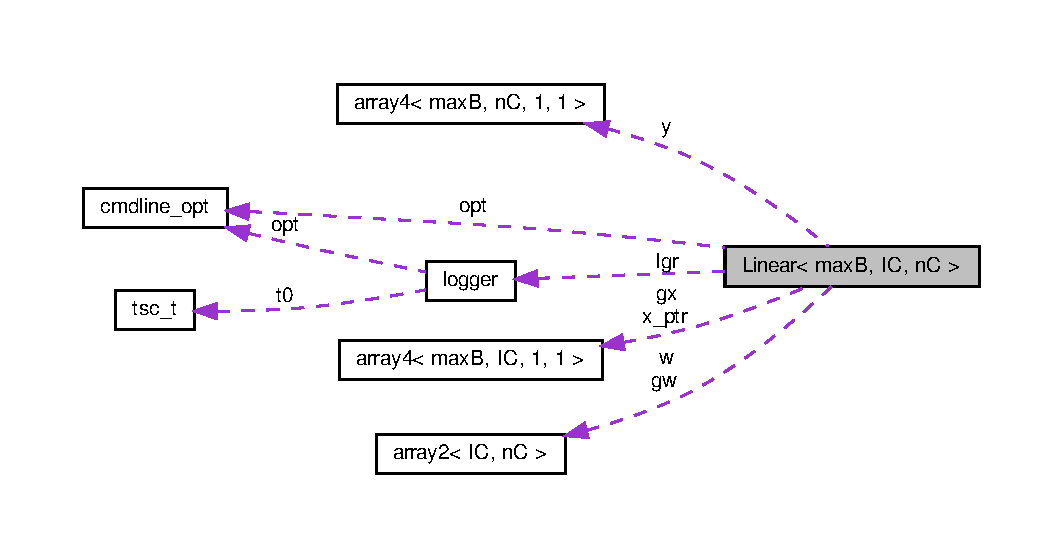
\includegraphics[width=350pt]{structLinear__coll__graph}
\end{center}
\end{figure}
\subsection*{Public Member Functions}
\begin{DoxyCompactItemize}
\item 
void \hyperlink{structLinear_a45f2c4c010a2451d39e0a7e736fd4a58}{init} (\hyperlink{structcmdline__opt}{cmdline\+\_\+opt} \hyperlink{structLinear_ad6b0173f0baf5ce07b3cd7340d4ed0d4}{opt}, \hyperlink{structlogger}{logger} $\ast$\hyperlink{structLinear_acde13832b627b3c1113283e22bac77a7}{lgr}, \hyperlink{structrnd__gen__t}{rnd\+\_\+gen\+\_\+t} \&rg)
\begin{DoxyCompactList}\small\item\em initialize \end{DoxyCompactList}\item 
\hyperlink{structLinear}{Linear}$<$ maxB, IC, nC $>$ $\ast$ \hyperlink{structLinear_a0c7811cf3a3731974b668f7e973a79f4}{copy} ()
\begin{DoxyCompactList}\small\item\em make a copy of this \end{DoxyCompactList}\item 
void \hyperlink{structLinear_a0c6dcb67669d4984b6b9a676d4f14177}{set\+\_\+dev} (\hyperlink{structLinear}{Linear}$<$ maxB, IC, nC $>$ $\ast$\hyperlink{structLinear_a84bf1832fbbaccc87ca3e13b45f5acb4}{dev})
\begin{DoxyCompactList}\small\item\em set the device pointer for this and all subobjects \end{DoxyCompactList}\item 
void \hyperlink{structLinear_aecf7edf669cf1182b49b604a2c9b3212}{make\+\_\+dev} ()
\begin{DoxyCompactList}\small\item\em if the algorithm is a gpu algorithm, allocate a device shadow of this object and set dev field of this and all subobjects. otherwise it sets all dev fields to null. \end{DoxyCompactList}\item 
void \hyperlink{structLinear_ad691fa515105ec71c69eed5f0ae03af6}{del\+\_\+dev} ()
\begin{DoxyCompactList}\small\item\em if the algorithm is a gpu algorithm, dev field must not be null and deallocate it. \end{DoxyCompactList}\item 
\mbox{\Hypertarget{structLinear_a36c57d7c3b7e25ae73f8bc3b5bb49992}\label{structLinear_a36c57d7c3b7e25ae73f8bc3b5bb49992}} 
void \hyperlink{structLinear_a36c57d7c3b7e25ae73f8bc3b5bb49992}{to\+\_\+dev} ()
\begin{DoxyCompactList}\small\item\em if the algorithm is a gpu algorithm, dev field must not be null and send the host data to the device memory \end{DoxyCompactList}\item 
\mbox{\Hypertarget{structLinear_a2cf0ae6b25a12dbe31194a283e075feb}\label{structLinear_a2cf0ae6b25a12dbe31194a283e075feb}} 
void \hyperlink{structLinear_a2cf0ae6b25a12dbe31194a283e075feb}{to\+\_\+host} ()
\begin{DoxyCompactList}\small\item\em if the algorithm is a gpu algorithm, dev field must not be null and send the device data to the host memory \end{DoxyCompactList}\item 
\+\_\+\+\_\+device\+\_\+\+\_\+ \+\_\+\+\_\+host\+\_\+\+\_\+ void \hyperlink{structLinear_aa59e1addd962ac7a70993229534ab899}{update\+\_\+base} (\hyperlink{vgg__util_8h_a1082d08aaa761215ec83e7149f27ad16}{real} eta)
\begin{DoxyCompactList}\small\item\em the baseline (serial) implementation of update called both by cpu implementation (update\+\_\+cpu) and gpu implementation (update\+\_\+dev). the call sequence update -\/$>$ update\+\_\+cpu -\/$>$ update\+\_\+base on cpu and and is update -\/$>$ update\+\_\+gpu -\/$>$ update\+\_\+global -\/$>$ update\+\_\+dev -\/$>$ update\+\_\+base \end{DoxyCompactList}\item 
\+\_\+\+\_\+device\+\_\+\+\_\+ void \hyperlink{structLinear_ad45413b0c13ca0ca89db6a3217a8b00b}{update\+\_\+dev} (\hyperlink{vgg__util_8h_a1082d08aaa761215ec83e7149f27ad16}{real} eta)
\begin{DoxyCompactList}\small\item\em the device function of update called from the global (non-\/member) function \end{DoxyCompactList}\item 
void \hyperlink{structLinear_a8ca71565731b9d8c3ba552578c61753a}{update\+\_\+gpu} (\hyperlink{vgg__util_8h_a1082d08aaa761215ec83e7149f27ad16}{real} eta)
\begin{DoxyCompactList}\small\item\em a gpu version of baseline code called from the entry function (update) \end{DoxyCompactList}\item 
void \hyperlink{structLinear_afabe5b3388c37c5b02e9f7ca7f0cd686}{update\+\_\+cpu} (\hyperlink{vgg__util_8h_a1082d08aaa761215ec83e7149f27ad16}{real} eta)
\begin{DoxyCompactList}\small\item\em a cpu version of baseline code called from the entry function (update) \end{DoxyCompactList}\item 
void \hyperlink{structLinear_a828a72af0a1ccac904325ee280dbefa4}{update} (\hyperlink{vgg__util_8h_a1082d08aaa761215ec83e7149f27ad16}{real} eta)
\begin{DoxyCompactList}\small\item\em update weights of all sublayers with gradients that must have been computed \end{DoxyCompactList}\item 
\+\_\+\+\_\+device\+\_\+\+\_\+ \+\_\+\+\_\+host\+\_\+\+\_\+ void \hyperlink{structLinear_adb02d44e0558e4e26b9a550945cd3b7e}{forward\+\_\+base} (\hyperlink{structarray4}{array4}$<$ maxB, IC, 1, 1 $>$ \&x)
\begin{DoxyCompactList}\small\item\em the baseline (serial) implementation of forward called both by cpu implementation (forward\+\_\+cpu) and gpu implementation (forward\+\_\+dev). the call sequence forward -\/$>$ forward\+\_\+cpu -\/$>$ forward\+\_\+base on cpu and and is forward -\/$>$ forward\+\_\+gpu -\/$>$ forward\+\_\+global -\/$>$ forward\+\_\+dev -\/$>$ forward\+\_\+base \end{DoxyCompactList}\item 
\+\_\+\+\_\+device\+\_\+\+\_\+ void \hyperlink{structLinear_a2b86dba92137500810cbf3ed95ee1fcb}{forward\+\_\+dev} (\hyperlink{structarray4}{array4}$<$ maxB, IC, 1, 1 $>$ \&x)
\begin{DoxyCompactList}\small\item\em the device function of forward called from the global (non-\/member) function \end{DoxyCompactList}\item 
void \hyperlink{structLinear_a1d794073640bad48f9722f5d40b98902}{forward\+\_\+gpu} (\hyperlink{structarray4}{array4}$<$ maxB, IC, 1, 1 $>$ \&x)
\begin{DoxyCompactList}\small\item\em a gpu version of baseline code called from the entry function (forward) \end{DoxyCompactList}\item 
void \hyperlink{structLinear_a02f18ced52dc4bd6aa0ea45119c6a7e0}{forward\+\_\+cpu} (\hyperlink{structarray4}{array4}$<$ maxB, IC, 1, 1 $>$ \&x)
\begin{DoxyCompactList}\small\item\em a cpu version of baseline code called from the entry function (forward) \end{DoxyCompactList}\item 
\hyperlink{structarray4}{array4}$<$ maxB, nC, 1, 1 $>$ \& \hyperlink{structLinear_aed0294f2d1c2013f66d89a52474352e5}{forward} (\hyperlink{structarray4}{array4}$<$ maxB, IC, 1, 1 $>$ \&x)
\begin{DoxyCompactList}\small\item\em calc the loss function of a mini-\/batch (x) \end{DoxyCompactList}\item 
\+\_\+\+\_\+device\+\_\+\+\_\+ \+\_\+\+\_\+host\+\_\+\+\_\+ void \hyperlink{structLinear_adcabfb5486aad2c05dd94bae98acf168}{backward\+\_\+base} (\hyperlink{structarray4}{array4}$<$ maxB, nC, 1, 1 $>$ \&gy)
\begin{DoxyCompactList}\small\item\em the baseline (serial) implementation of backward called both by cpu implementation (backward\+\_\+cpu) and gpu implementation (backward\+\_\+dev). the call sequence backward -\/$>$ backward\+\_\+cpu -\/$>$ backward\+\_\+base on cpu and and is backward -\/$>$ backward\+\_\+gpu -\/$>$ backward\+\_\+global -\/$>$ backward\+\_\+dev -\/$>$ backward\+\_\+base \end{DoxyCompactList}\item 
\+\_\+\+\_\+device\+\_\+\+\_\+ void \hyperlink{structLinear_a865f8dedc402675cd5cf240fcfbcd258}{backward\+\_\+dev} (\hyperlink{structarray4}{array4}$<$ maxB, nC, 1, 1 $>$ \&gy)
\begin{DoxyCompactList}\small\item\em the device function of backward called from the global (non-\/member) function \end{DoxyCompactList}\item 
void \hyperlink{structLinear_acc4936542d24da1357c1c7fb7f95d6ea}{backward\+\_\+gpu} (\hyperlink{structarray4}{array4}$<$ maxB, nC, 1, 1 $>$ \&gy)
\begin{DoxyCompactList}\small\item\em a gpu version of baseline code called from the entry function (backward) \end{DoxyCompactList}\item 
void \hyperlink{structLinear_acd4bd03ccec0da8849c2536d32770a61}{backward\+\_\+cpu} (\hyperlink{structarray4}{array4}$<$ maxB, nC, 1, 1 $>$ \&gy)
\begin{DoxyCompactList}\small\item\em a cpu version of baseline code called from the entry function (backward) \end{DoxyCompactList}\item 
\hyperlink{structarray4}{array4}$<$ maxB, IC, 1, 1 $>$ \& \hyperlink{structLinear_aeaa39d38b876fbd70794621955193fd3}{backward} (\hyperlink{structarray4}{array4}$<$ maxB, nC, 1, 1 $>$ \&gy)
\begin{DoxyCompactList}\small\item\em calc the gradient of loss wrt the input (x) \end{DoxyCompactList}\item 
void \hyperlink{structLinear_aab38b786325b4701080a89d5dab96f23}{rand\+\_\+grad} (\hyperlink{structrnd__gen__t}{rnd\+\_\+gen\+\_\+t} \&rg, \hyperlink{vgg__util_8h_a1082d08aaa761215ec83e7149f27ad16}{real} p, \hyperlink{vgg__util_8h_a1082d08aaa761215ec83e7149f27ad16}{real} q)
\begin{DoxyCompactList}\small\item\em randomly set all gradients to values between p and q \end{DoxyCompactList}\item 
void \hyperlink{structLinear_a4faa818e70d779b80663b361a1e7ef75}{set\+\_\+grad} (\hyperlink{structLinear}{Linear}$<$ maxB, IC, nC $>$ \&o)
\begin{DoxyCompactList}\small\item\em set all gradients to gradients of another object \end{DoxyCompactList}\item 
\hyperlink{vgg__util_8h_a1082d08aaa761215ec83e7149f27ad16}{real} \hyperlink{structLinear_af920adb0c630cddb4f8012984784807c}{gw\+\_\+dot\+\_\+gw} (\hyperlink{structLinear}{Linear}$<$ maxB, IC, nC $>$ \&o)
\begin{DoxyCompactList}\small\item\em take the inner product of gradients \end{DoxyCompactList}\end{DoxyCompactItemize}
\subsection*{Public Attributes}
\begin{DoxyCompactItemize}
\item 
\hyperlink{structLinear}{Linear}$<$ maxB, IC, nC $>$ $\ast$ \hyperlink{structLinear_a84bf1832fbbaccc87ca3e13b45f5acb4}{dev}
\item 
\hyperlink{structcmdline__opt}{cmdline\+\_\+opt} \hyperlink{structLinear_ad6b0173f0baf5ce07b3cd7340d4ed0d4}{opt}
\item 
\hyperlink{structlogger}{logger} $\ast$ \hyperlink{structLinear_acde13832b627b3c1113283e22bac77a7}{lgr}
\item 
\hyperlink{structarray4}{array4}$<$ maxB, IC, 1, 1 $>$ $\ast$ \hyperlink{structLinear_a8a7c8ecf358de5e00589a722a0c4541c}{x\+\_\+ptr}
\item 
\hyperlink{structarray2}{array2}$<$ IC, nC $>$ \hyperlink{structLinear_a5abe6ceff587b423273808d94b392ee8}{w}
\item 
\hyperlink{structarray4}{array4}$<$ maxB, nC, 1, 1 $>$ \hyperlink{structLinear_a422f2130612692682fdd151b96899264}{y}
\item 
\hyperlink{structarray2}{array2}$<$ IC, nC $>$ \hyperlink{structLinear_a62267914d63b5f94379e4f9caf6b317c}{gw}
\item 
\hyperlink{structarray4}{array4}$<$ maxB, IC, 1, 1 $>$ \hyperlink{structLinear_abcdbaef350ab7abbcb459cfa87961bba}{gx}
\end{DoxyCompactItemize}


\subsection{Detailed Description}
\subsubsection*{template$<$idx\+\_\+t maxB, idx\+\_\+t IC, idx\+\_\+t nC$>$\newline
struct Linear$<$ max\+B, I\+C, n\+C $>$}

linear (fully connected) layer 


\begin{DoxyParams}{Parameters}
{\em (max\+B)} & the maximum number of images (batch size) \\
\hline
{\em (\+I\+C)} & the number of channels per input image (the original input has typically three channels for R\+GB. in hidden layers, it starts from 64 and goes up to 512 in the last hidden layer) \\
\hline
{\em (n\+C)} & number of classes (10) \\
\hline
\end{DoxyParams}


\subsection{Member Function Documentation}
\mbox{\Hypertarget{structLinear_aeaa39d38b876fbd70794621955193fd3}\label{structLinear_aeaa39d38b876fbd70794621955193fd3}} 
\index{Linear@{Linear}!backward@{backward}}
\index{backward@{backward}!Linear@{Linear}}
\subsubsection{\texorpdfstring{backward()}{backward()}}
{\footnotesize\ttfamily template$<$idx\+\_\+t maxB, idx\+\_\+t IC, idx\+\_\+t nC$>$ \\
\hyperlink{structarray4}{array4}$<$maxB,IC,1,1$>$\& \hyperlink{structLinear}{Linear}$<$ maxB, IC, nC $>$\+::backward (\begin{DoxyParamCaption}\item[{\hyperlink{structarray4}{array4}$<$ maxB, nC, 1, 1 $>$ \&}]{gy }\end{DoxyParamCaption})\hspace{0.3cm}{\ttfamily [inline]}}



calc the gradient of loss wrt the input (x) 


\begin{DoxyParams}{Parameters}
{\em (gy)} & gradient of loss with respect to the output\\
\hline
\end{DoxyParams}
calc the gradient of loss wrt the input. along the way, it also calculates the gradient of loss wrt weights for all sublayers that have weights. since this is the entire network, gy is actually a vector whose components are all 1. (loss = sum of losses of each data). \begin{DoxySeeAlso}{See also}
\hyperlink{structLinear_aed0294f2d1c2013f66d89a52474352e5}{forward} 

\hyperlink{structLinear_a828a72af0a1ccac904325ee280dbefa4}{update} 
\end{DoxySeeAlso}
\mbox{\Hypertarget{structLinear_adcabfb5486aad2c05dd94bae98acf168}\label{structLinear_adcabfb5486aad2c05dd94bae98acf168}} 
\index{Linear@{Linear}!backward\+\_\+base@{backward\+\_\+base}}
\index{backward\+\_\+base@{backward\+\_\+base}!Linear@{Linear}}
\subsubsection{\texorpdfstring{backward\+\_\+base()}{backward\_base()}}
{\footnotesize\ttfamily template$<$idx\+\_\+t maxB, idx\+\_\+t IC, idx\+\_\+t nC$>$ \\
\+\_\+\+\_\+device\+\_\+\+\_\+ \+\_\+\+\_\+host\+\_\+\+\_\+ void \hyperlink{structLinear}{Linear}$<$ maxB, IC, nC $>$\+::backward\+\_\+base (\begin{DoxyParamCaption}\item[{\hyperlink{structarray4}{array4}$<$ maxB, nC, 1, 1 $>$ \&}]{gy }\end{DoxyParamCaption})\hspace{0.3cm}{\ttfamily [inline]}}



the baseline (serial) implementation of backward called both by cpu implementation (backward\+\_\+cpu) and gpu implementation (backward\+\_\+dev). the call sequence backward -\/$>$ backward\+\_\+cpu -\/$>$ backward\+\_\+base on cpu and and is backward -\/$>$ backward\+\_\+gpu -\/$>$ backward\+\_\+global -\/$>$ backward\+\_\+dev -\/$>$ backward\+\_\+base 


\begin{DoxyParams}{Parameters}
{\em (gy)} & gradient of loss with respect to the output \\
\hline
\end{DoxyParams}
\begin{DoxySeeAlso}{See also}
\hyperlink{structLinear_aeaa39d38b876fbd70794621955193fd3}{backward} 

\hyperlink{structLinear_acc4936542d24da1357c1c7fb7f95d6ea}{backward\+\_\+gpu} 

\hyperlink{softmaxcrossentropy_8h_a47d56a9a23e08247b227f4aac17413e0}{backward\+\_\+global} 

\hyperlink{structLinear_a865f8dedc402675cd5cf240fcfbcd258}{backward\+\_\+dev} 
\end{DoxySeeAlso}
\mbox{\Hypertarget{structLinear_acd4bd03ccec0da8849c2536d32770a61}\label{structLinear_acd4bd03ccec0da8849c2536d32770a61}} 
\index{Linear@{Linear}!backward\+\_\+cpu@{backward\+\_\+cpu}}
\index{backward\+\_\+cpu@{backward\+\_\+cpu}!Linear@{Linear}}
\subsubsection{\texorpdfstring{backward\+\_\+cpu()}{backward\_cpu()}}
{\footnotesize\ttfamily template$<$idx\+\_\+t maxB, idx\+\_\+t IC, idx\+\_\+t nC$>$ \\
void \hyperlink{structLinear}{Linear}$<$ maxB, IC, nC $>$\+::backward\+\_\+cpu (\begin{DoxyParamCaption}\item[{\hyperlink{structarray4}{array4}$<$ maxB, nC, 1, 1 $>$ \&}]{gy }\end{DoxyParamCaption})\hspace{0.3cm}{\ttfamily [inline]}}



a cpu version of baseline code called from the entry function (backward) 


\begin{DoxyParams}{Parameters}
{\em (gy)} & gradient of loss with respect to the output \\
\hline
\end{DoxyParams}
\begin{DoxySeeAlso}{See also}
\hyperlink{structLinear_aeaa39d38b876fbd70794621955193fd3}{backward} 

\hyperlink{structLinear_adcabfb5486aad2c05dd94bae98acf168}{backward\+\_\+base} 
\end{DoxySeeAlso}
\mbox{\Hypertarget{structLinear_a865f8dedc402675cd5cf240fcfbcd258}\label{structLinear_a865f8dedc402675cd5cf240fcfbcd258}} 
\index{Linear@{Linear}!backward\+\_\+dev@{backward\+\_\+dev}}
\index{backward\+\_\+dev@{backward\+\_\+dev}!Linear@{Linear}}
\subsubsection{\texorpdfstring{backward\+\_\+dev()}{backward\_dev()}}
{\footnotesize\ttfamily template$<$idx\+\_\+t maxB, idx\+\_\+t IC, idx\+\_\+t nC$>$ \\
\+\_\+\+\_\+device\+\_\+\+\_\+ void \hyperlink{structLinear}{Linear}$<$ maxB, IC, nC $>$\+::backward\+\_\+dev (\begin{DoxyParamCaption}\item[{\hyperlink{structarray4}{array4}$<$ maxB, nC, 1, 1 $>$ \&}]{gy }\end{DoxyParamCaption})\hspace{0.3cm}{\ttfamily [inline]}}



the device function of backward called from the global (non-\/member) function 


\begin{DoxyParams}{Parameters}
{\em (gy)} & gradient of loss with respect to the output \\
\hline
\end{DoxyParams}
\begin{DoxySeeAlso}{See also}
\hyperlink{structLinear_aeaa39d38b876fbd70794621955193fd3}{backward} 

\hyperlink{structLinear_acc4936542d24da1357c1c7fb7f95d6ea}{backward\+\_\+gpu} 

\hyperlink{softmaxcrossentropy_8h_a47d56a9a23e08247b227f4aac17413e0}{backward\+\_\+global} 

\hyperlink{structLinear_adcabfb5486aad2c05dd94bae98acf168}{backward\+\_\+base} 
\end{DoxySeeAlso}
\mbox{\Hypertarget{structLinear_acc4936542d24da1357c1c7fb7f95d6ea}\label{structLinear_acc4936542d24da1357c1c7fb7f95d6ea}} 
\index{Linear@{Linear}!backward\+\_\+gpu@{backward\+\_\+gpu}}
\index{backward\+\_\+gpu@{backward\+\_\+gpu}!Linear@{Linear}}
\subsubsection{\texorpdfstring{backward\+\_\+gpu()}{backward\_gpu()}}
{\footnotesize\ttfamily template$<$idx\+\_\+t maxB, idx\+\_\+t IC, idx\+\_\+t nC$>$ \\
void \hyperlink{structLinear}{Linear}$<$ maxB, IC, nC $>$\+::backward\+\_\+gpu (\begin{DoxyParamCaption}\item[{\hyperlink{structarray4}{array4}$<$ maxB, nC, 1, 1 $>$ \&}]{gy }\end{DoxyParamCaption})\hspace{0.3cm}{\ttfamily [inline]}}



a gpu version of baseline code called from the entry function (backward) 


\begin{DoxyParams}{Parameters}
{\em (gy)} & gradient of loss with respect to the output \\
\hline
\end{DoxyParams}
\begin{DoxySeeAlso}{See also}
\hyperlink{structLinear_aeaa39d38b876fbd70794621955193fd3}{backward} 

\hyperlink{softmaxcrossentropy_8h_a47d56a9a23e08247b227f4aac17413e0}{backward\+\_\+global} 

\hyperlink{structLinear_a865f8dedc402675cd5cf240fcfbcd258}{backward\+\_\+dev} 

\hyperlink{structLinear_adcabfb5486aad2c05dd94bae98acf168}{backward\+\_\+base} 
\end{DoxySeeAlso}
\mbox{\Hypertarget{structLinear_a0c7811cf3a3731974b668f7e973a79f4}\label{structLinear_a0c7811cf3a3731974b668f7e973a79f4}} 
\index{Linear@{Linear}!copy@{copy}}
\index{copy@{copy}!Linear@{Linear}}
\subsubsection{\texorpdfstring{copy()}{copy()}}
{\footnotesize\ttfamily template$<$idx\+\_\+t maxB, idx\+\_\+t IC, idx\+\_\+t nC$>$ \\
\hyperlink{structLinear}{Linear}$<$maxB,IC,nC$>$$\ast$ \hyperlink{structLinear}{Linear}$<$ maxB, IC, nC $>$\+::copy (\begin{DoxyParamCaption}{ }\end{DoxyParamCaption})\hspace{0.3cm}{\ttfamily [inline]}}



make a copy of this 

if this object has a device pointer, the copy will have a device pointer too, but its contents are N\+OT copied \mbox{\Hypertarget{structLinear_ad691fa515105ec71c69eed5f0ae03af6}\label{structLinear_ad691fa515105ec71c69eed5f0ae03af6}} 
\index{Linear@{Linear}!del\+\_\+dev@{del\+\_\+dev}}
\index{del\+\_\+dev@{del\+\_\+dev}!Linear@{Linear}}
\subsubsection{\texorpdfstring{del\+\_\+dev()}{del\_dev()}}
{\footnotesize\ttfamily template$<$idx\+\_\+t maxB, idx\+\_\+t IC, idx\+\_\+t nC$>$ \\
void \hyperlink{structLinear}{Linear}$<$ maxB, IC, nC $>$\+::del\+\_\+dev (\begin{DoxyParamCaption}{ }\end{DoxyParamCaption})\hspace{0.3cm}{\ttfamily [inline]}}



if the algorithm is a gpu algorithm, dev field must not be null and deallocate it. 

\begin{DoxySeeAlso}{See also}
\hyperlink{structLinear_aecf7edf669cf1182b49b604a2c9b3212}{make\+\_\+dev} 

\hyperlink{structLinear_a0c6dcb67669d4984b6b9a676d4f14177}{set\+\_\+dev} 
\end{DoxySeeAlso}
\mbox{\Hypertarget{structLinear_aed0294f2d1c2013f66d89a52474352e5}\label{structLinear_aed0294f2d1c2013f66d89a52474352e5}} 
\index{Linear@{Linear}!forward@{forward}}
\index{forward@{forward}!Linear@{Linear}}
\subsubsection{\texorpdfstring{forward()}{forward()}}
{\footnotesize\ttfamily template$<$idx\+\_\+t maxB, idx\+\_\+t IC, idx\+\_\+t nC$>$ \\
\hyperlink{structarray4}{array4}$<$maxB,nC,1,1$>$\& \hyperlink{structLinear}{Linear}$<$ maxB, IC, nC $>$\+::forward (\begin{DoxyParamCaption}\item[{\hyperlink{structarray4}{array4}$<$ maxB, IC, 1, 1 $>$ \&}]{x }\end{DoxyParamCaption})\hspace{0.3cm}{\ttfamily [inline]}}



calc the loss function of a mini-\/batch (x) 


\begin{DoxyParams}{Parameters}
{\em (x)} & input images \\
\hline
\end{DoxyParams}
\begin{DoxySeeAlso}{See also}
\hyperlink{structLinear_aeaa39d38b876fbd70794621955193fd3}{backward} 

\hyperlink{structLinear_a828a72af0a1ccac904325ee280dbefa4}{update} 
\end{DoxySeeAlso}
\mbox{\Hypertarget{structLinear_adb02d44e0558e4e26b9a550945cd3b7e}\label{structLinear_adb02d44e0558e4e26b9a550945cd3b7e}} 
\index{Linear@{Linear}!forward\+\_\+base@{forward\+\_\+base}}
\index{forward\+\_\+base@{forward\+\_\+base}!Linear@{Linear}}
\subsubsection{\texorpdfstring{forward\+\_\+base()}{forward\_base()}}
{\footnotesize\ttfamily template$<$idx\+\_\+t maxB, idx\+\_\+t IC, idx\+\_\+t nC$>$ \\
\+\_\+\+\_\+device\+\_\+\+\_\+ \+\_\+\+\_\+host\+\_\+\+\_\+ void \hyperlink{structLinear}{Linear}$<$ maxB, IC, nC $>$\+::forward\+\_\+base (\begin{DoxyParamCaption}\item[{\hyperlink{structarray4}{array4}$<$ maxB, IC, 1, 1 $>$ \&}]{x }\end{DoxyParamCaption})\hspace{0.3cm}{\ttfamily [inline]}}



the baseline (serial) implementation of forward called both by cpu implementation (forward\+\_\+cpu) and gpu implementation (forward\+\_\+dev). the call sequence forward -\/$>$ forward\+\_\+cpu -\/$>$ forward\+\_\+base on cpu and and is forward -\/$>$ forward\+\_\+gpu -\/$>$ forward\+\_\+global -\/$>$ forward\+\_\+dev -\/$>$ forward\+\_\+base 


\begin{DoxyParams}{Parameters}
{\em (x)} & input images \\
\hline
\end{DoxyParams}
\begin{DoxySeeAlso}{See also}
\hyperlink{structLinear_aed0294f2d1c2013f66d89a52474352e5}{forward} 

\hyperlink{structLinear_a1d794073640bad48f9722f5d40b98902}{forward\+\_\+gpu} 

\hyperlink{softmaxcrossentropy_8h_a578aeeb166bd06e800d9b396eab48b35}{forward\+\_\+global} 

\hyperlink{structLinear_a2b86dba92137500810cbf3ed95ee1fcb}{forward\+\_\+dev} 
\end{DoxySeeAlso}
\mbox{\Hypertarget{structLinear_a02f18ced52dc4bd6aa0ea45119c6a7e0}\label{structLinear_a02f18ced52dc4bd6aa0ea45119c6a7e0}} 
\index{Linear@{Linear}!forward\+\_\+cpu@{forward\+\_\+cpu}}
\index{forward\+\_\+cpu@{forward\+\_\+cpu}!Linear@{Linear}}
\subsubsection{\texorpdfstring{forward\+\_\+cpu()}{forward\_cpu()}}
{\footnotesize\ttfamily template$<$idx\+\_\+t maxB, idx\+\_\+t IC, idx\+\_\+t nC$>$ \\
void \hyperlink{structLinear}{Linear}$<$ maxB, IC, nC $>$\+::forward\+\_\+cpu (\begin{DoxyParamCaption}\item[{\hyperlink{structarray4}{array4}$<$ maxB, IC, 1, 1 $>$ \&}]{x }\end{DoxyParamCaption})\hspace{0.3cm}{\ttfamily [inline]}}



a cpu version of baseline code called from the entry function (forward) 


\begin{DoxyParams}{Parameters}
{\em (x)} & input images \\
\hline
\end{DoxyParams}
\begin{DoxySeeAlso}{See also}
\hyperlink{structLinear_aed0294f2d1c2013f66d89a52474352e5}{forward} 

\hyperlink{structLinear_adb02d44e0558e4e26b9a550945cd3b7e}{forward\+\_\+base} 
\end{DoxySeeAlso}
\mbox{\Hypertarget{structLinear_a2b86dba92137500810cbf3ed95ee1fcb}\label{structLinear_a2b86dba92137500810cbf3ed95ee1fcb}} 
\index{Linear@{Linear}!forward\+\_\+dev@{forward\+\_\+dev}}
\index{forward\+\_\+dev@{forward\+\_\+dev}!Linear@{Linear}}
\subsubsection{\texorpdfstring{forward\+\_\+dev()}{forward\_dev()}}
{\footnotesize\ttfamily template$<$idx\+\_\+t maxB, idx\+\_\+t IC, idx\+\_\+t nC$>$ \\
\+\_\+\+\_\+device\+\_\+\+\_\+ void \hyperlink{structLinear}{Linear}$<$ maxB, IC, nC $>$\+::forward\+\_\+dev (\begin{DoxyParamCaption}\item[{\hyperlink{structarray4}{array4}$<$ maxB, IC, 1, 1 $>$ \&}]{x }\end{DoxyParamCaption})\hspace{0.3cm}{\ttfamily [inline]}}



the device function of forward called from the global (non-\/member) function 


\begin{DoxyParams}{Parameters}
{\em (x)} & input images \\
\hline
\end{DoxyParams}
\begin{DoxySeeAlso}{See also}
\hyperlink{structLinear_aed0294f2d1c2013f66d89a52474352e5}{forward} 

\hyperlink{structLinear_a1d794073640bad48f9722f5d40b98902}{forward\+\_\+gpu} 

\hyperlink{softmaxcrossentropy_8h_a578aeeb166bd06e800d9b396eab48b35}{forward\+\_\+global} 

\hyperlink{structLinear_adb02d44e0558e4e26b9a550945cd3b7e}{forward\+\_\+base} 
\end{DoxySeeAlso}
\mbox{\Hypertarget{structLinear_a1d794073640bad48f9722f5d40b98902}\label{structLinear_a1d794073640bad48f9722f5d40b98902}} 
\index{Linear@{Linear}!forward\+\_\+gpu@{forward\+\_\+gpu}}
\index{forward\+\_\+gpu@{forward\+\_\+gpu}!Linear@{Linear}}
\subsubsection{\texorpdfstring{forward\+\_\+gpu()}{forward\_gpu()}}
{\footnotesize\ttfamily template$<$idx\+\_\+t maxB, idx\+\_\+t IC, idx\+\_\+t nC$>$ \\
void \hyperlink{structLinear}{Linear}$<$ maxB, IC, nC $>$\+::forward\+\_\+gpu (\begin{DoxyParamCaption}\item[{\hyperlink{structarray4}{array4}$<$ maxB, IC, 1, 1 $>$ \&}]{x }\end{DoxyParamCaption})\hspace{0.3cm}{\ttfamily [inline]}}



a gpu version of baseline code called from the entry function (forward) 


\begin{DoxyParams}{Parameters}
{\em (x)} & input images \\
\hline
\end{DoxyParams}
\begin{DoxySeeAlso}{See also}
\hyperlink{structLinear_aed0294f2d1c2013f66d89a52474352e5}{forward} 

\hyperlink{softmaxcrossentropy_8h_a578aeeb166bd06e800d9b396eab48b35}{forward\+\_\+global} 

\hyperlink{structLinear_a2b86dba92137500810cbf3ed95ee1fcb}{forward\+\_\+dev} 

\hyperlink{structLinear_adb02d44e0558e4e26b9a550945cd3b7e}{forward\+\_\+base} 
\end{DoxySeeAlso}
\mbox{\Hypertarget{structLinear_af920adb0c630cddb4f8012984784807c}\label{structLinear_af920adb0c630cddb4f8012984784807c}} 
\index{Linear@{Linear}!gw\+\_\+dot\+\_\+gw@{gw\+\_\+dot\+\_\+gw}}
\index{gw\+\_\+dot\+\_\+gw@{gw\+\_\+dot\+\_\+gw}!Linear@{Linear}}
\subsubsection{\texorpdfstring{gw\+\_\+dot\+\_\+gw()}{gw\_dot\_gw()}}
{\footnotesize\ttfamily template$<$idx\+\_\+t maxB, idx\+\_\+t IC, idx\+\_\+t nC$>$ \\
\hyperlink{vgg__util_8h_a1082d08aaa761215ec83e7149f27ad16}{real} \hyperlink{structLinear}{Linear}$<$ maxB, IC, nC $>$\+::gw\+\_\+dot\+\_\+gw (\begin{DoxyParamCaption}\item[{\hyperlink{structLinear}{Linear}$<$ maxB, IC, nC $>$ \&}]{o }\end{DoxyParamCaption})\hspace{0.3cm}{\ttfamily [inline]}}



take the inner product of gradients 


\begin{DoxyParams}{Parameters}
{\em (o)} & the object to take the inner product with\\
\hline
\end{DoxyParams}
take the inner product of this object\textquotesingle{}s gradients and b\textquotesingle{}s gradients \mbox{\Hypertarget{structLinear_a45f2c4c010a2451d39e0a7e736fd4a58}\label{structLinear_a45f2c4c010a2451d39e0a7e736fd4a58}} 
\index{Linear@{Linear}!init@{init}}
\index{init@{init}!Linear@{Linear}}
\subsubsection{\texorpdfstring{init()}{init()}}
{\footnotesize\ttfamily template$<$idx\+\_\+t maxB, idx\+\_\+t IC, idx\+\_\+t nC$>$ \\
void \hyperlink{structLinear}{Linear}$<$ maxB, IC, nC $>$\+::init (\begin{DoxyParamCaption}\item[{\hyperlink{structcmdline__opt}{cmdline\+\_\+opt}}]{opt,  }\item[{\hyperlink{structlogger}{logger} $\ast$}]{lgr,  }\item[{\hyperlink{structrnd__gen__t}{rnd\+\_\+gen\+\_\+t} \&}]{rg }\end{DoxyParamCaption})\hspace{0.3cm}{\ttfamily [inline]}}



initialize 


\begin{DoxyParams}{Parameters}
{\em (opt)} & command line options \\
\hline
{\em (lgr)} & logger \\
\hline
{\em (rg)} & random number generator for initializing weights \\
\hline
\end{DoxyParams}
\mbox{\Hypertarget{structLinear_aecf7edf669cf1182b49b604a2c9b3212}\label{structLinear_aecf7edf669cf1182b49b604a2c9b3212}} 
\index{Linear@{Linear}!make\+\_\+dev@{make\+\_\+dev}}
\index{make\+\_\+dev@{make\+\_\+dev}!Linear@{Linear}}
\subsubsection{\texorpdfstring{make\+\_\+dev()}{make\_dev()}}
{\footnotesize\ttfamily template$<$idx\+\_\+t maxB, idx\+\_\+t IC, idx\+\_\+t nC$>$ \\
void \hyperlink{structLinear}{Linear}$<$ maxB, IC, nC $>$\+::make\+\_\+dev (\begin{DoxyParamCaption}{ }\end{DoxyParamCaption})\hspace{0.3cm}{\ttfamily [inline]}}



if the algorithm is a gpu algorithm, allocate a device shadow of this object and set dev field of this and all subobjects. otherwise it sets all dev fields to null. 

\begin{DoxySeeAlso}{See also}
\hyperlink{structLinear_a0c6dcb67669d4984b6b9a676d4f14177}{set\+\_\+dev} 

\hyperlink{structLinear_ad691fa515105ec71c69eed5f0ae03af6}{del\+\_\+dev} 
\end{DoxySeeAlso}
\mbox{\Hypertarget{structLinear_aab38b786325b4701080a89d5dab96f23}\label{structLinear_aab38b786325b4701080a89d5dab96f23}} 
\index{Linear@{Linear}!rand\+\_\+grad@{rand\+\_\+grad}}
\index{rand\+\_\+grad@{rand\+\_\+grad}!Linear@{Linear}}
\subsubsection{\texorpdfstring{rand\+\_\+grad()}{rand\_grad()}}
{\footnotesize\ttfamily template$<$idx\+\_\+t maxB, idx\+\_\+t IC, idx\+\_\+t nC$>$ \\
void \hyperlink{structLinear}{Linear}$<$ maxB, IC, nC $>$\+::rand\+\_\+grad (\begin{DoxyParamCaption}\item[{\hyperlink{structrnd__gen__t}{rnd\+\_\+gen\+\_\+t} \&}]{rg,  }\item[{\hyperlink{vgg__util_8h_a1082d08aaa761215ec83e7149f27ad16}{real}}]{p,  }\item[{\hyperlink{vgg__util_8h_a1082d08aaa761215ec83e7149f27ad16}{real}}]{q }\end{DoxyParamCaption})\hspace{0.3cm}{\ttfamily [inline]}}



randomly set all gradients to values between p and q 


\begin{DoxyParams}{Parameters}
{\em (rg)} & random number generator \\
\hline
{\em (p)} & minimum value of a component \\
\hline
{\em (q)} & maximum value of a component \\
\hline
\end{DoxyParams}
\mbox{\Hypertarget{structLinear_a0c6dcb67669d4984b6b9a676d4f14177}\label{structLinear_a0c6dcb67669d4984b6b9a676d4f14177}} 
\index{Linear@{Linear}!set\+\_\+dev@{set\+\_\+dev}}
\index{set\+\_\+dev@{set\+\_\+dev}!Linear@{Linear}}
\subsubsection{\texorpdfstring{set\+\_\+dev()}{set\_dev()}}
{\footnotesize\ttfamily template$<$idx\+\_\+t maxB, idx\+\_\+t IC, idx\+\_\+t nC$>$ \\
void \hyperlink{structLinear}{Linear}$<$ maxB, IC, nC $>$\+::set\+\_\+dev (\begin{DoxyParamCaption}\item[{\hyperlink{structLinear}{Linear}$<$ maxB, IC, nC $>$ $\ast$}]{dev }\end{DoxyParamCaption})\hspace{0.3cm}{\ttfamily [inline]}}



set the device pointer for this and all subobjects 


\begin{DoxyParams}{Parameters}
{\em (dev)} & a device memory or null \\
\hline
\end{DoxyParams}
\begin{DoxySeeAlso}{See also}
\hyperlink{structLinear_aecf7edf669cf1182b49b604a2c9b3212}{make\+\_\+dev} 

\hyperlink{structLinear_ad691fa515105ec71c69eed5f0ae03af6}{del\+\_\+dev}
\end{DoxySeeAlso}
if dev is not null, dev fields of all subojects point to the corresponding subjects in the device memory. if dev is not null, all dev fields become null. \mbox{\Hypertarget{structLinear_a4faa818e70d779b80663b361a1e7ef75}\label{structLinear_a4faa818e70d779b80663b361a1e7ef75}} 
\index{Linear@{Linear}!set\+\_\+grad@{set\+\_\+grad}}
\index{set\+\_\+grad@{set\+\_\+grad}!Linear@{Linear}}
\subsubsection{\texorpdfstring{set\+\_\+grad()}{set\_grad()}}
{\footnotesize\ttfamily template$<$idx\+\_\+t maxB, idx\+\_\+t IC, idx\+\_\+t nC$>$ \\
void \hyperlink{structLinear}{Linear}$<$ maxB, IC, nC $>$\+::set\+\_\+grad (\begin{DoxyParamCaption}\item[{\hyperlink{structLinear}{Linear}$<$ maxB, IC, nC $>$ \&}]{o }\end{DoxyParamCaption})\hspace{0.3cm}{\ttfamily [inline]}}



set all gradients to gradients of another object 


\begin{DoxyParams}{Parameters}
{\em (o)} & the object from which gradients get copied\\
\hline
\end{DoxyParams}
transfer gradients of o to this object \mbox{\Hypertarget{structLinear_a828a72af0a1ccac904325ee280dbefa4}\label{structLinear_a828a72af0a1ccac904325ee280dbefa4}} 
\index{Linear@{Linear}!update@{update}}
\index{update@{update}!Linear@{Linear}}
\subsubsection{\texorpdfstring{update()}{update()}}
{\footnotesize\ttfamily template$<$idx\+\_\+t maxB, idx\+\_\+t IC, idx\+\_\+t nC$>$ \\
void \hyperlink{structLinear}{Linear}$<$ maxB, IC, nC $>$\+::update (\begin{DoxyParamCaption}\item[{\hyperlink{vgg__util_8h_a1082d08aaa761215ec83e7149f27ad16}{real}}]{eta }\end{DoxyParamCaption})\hspace{0.3cm}{\ttfamily [inline]}}



update weights of all sublayers with gradients that must have been computed 


\begin{DoxyParams}{Parameters}
{\em (eta)} & the learning rate \\
\hline
\end{DoxyParams}
\begin{DoxySeeAlso}{See also}
\hyperlink{structLinear_aed0294f2d1c2013f66d89a52474352e5}{forward} 

\hyperlink{structLinear_aeaa39d38b876fbd70794621955193fd3}{backward} 
\end{DoxySeeAlso}
\mbox{\Hypertarget{structLinear_aa59e1addd962ac7a70993229534ab899}\label{structLinear_aa59e1addd962ac7a70993229534ab899}} 
\index{Linear@{Linear}!update\+\_\+base@{update\+\_\+base}}
\index{update\+\_\+base@{update\+\_\+base}!Linear@{Linear}}
\subsubsection{\texorpdfstring{update\+\_\+base()}{update\_base()}}
{\footnotesize\ttfamily template$<$idx\+\_\+t maxB, idx\+\_\+t IC, idx\+\_\+t nC$>$ \\
\+\_\+\+\_\+device\+\_\+\+\_\+ \+\_\+\+\_\+host\+\_\+\+\_\+ void \hyperlink{structLinear}{Linear}$<$ maxB, IC, nC $>$\+::update\+\_\+base (\begin{DoxyParamCaption}\item[{\hyperlink{vgg__util_8h_a1082d08aaa761215ec83e7149f27ad16}{real}}]{eta }\end{DoxyParamCaption})\hspace{0.3cm}{\ttfamily [inline]}}



the baseline (serial) implementation of update called both by cpu implementation (update\+\_\+cpu) and gpu implementation (update\+\_\+dev). the call sequence update -\/$>$ update\+\_\+cpu -\/$>$ update\+\_\+base on cpu and and is update -\/$>$ update\+\_\+gpu -\/$>$ update\+\_\+global -\/$>$ update\+\_\+dev -\/$>$ update\+\_\+base 


\begin{DoxyParams}{Parameters}
{\em (eta)} & the learning rate \\
\hline
\end{DoxyParams}
\begin{DoxySeeAlso}{See also}
\hyperlink{structLinear_a828a72af0a1ccac904325ee280dbefa4}{update} 

\hyperlink{structLinear_a8ca71565731b9d8c3ba552578c61753a}{update\+\_\+gpu} 

\hyperlink{linear_8h_a810703be28422bb9483665cbdbafd968}{update\+\_\+global} 

\hyperlink{structLinear_ad45413b0c13ca0ca89db6a3217a8b00b}{update\+\_\+dev} 
\end{DoxySeeAlso}
\mbox{\Hypertarget{structLinear_afabe5b3388c37c5b02e9f7ca7f0cd686}\label{structLinear_afabe5b3388c37c5b02e9f7ca7f0cd686}} 
\index{Linear@{Linear}!update\+\_\+cpu@{update\+\_\+cpu}}
\index{update\+\_\+cpu@{update\+\_\+cpu}!Linear@{Linear}}
\subsubsection{\texorpdfstring{update\+\_\+cpu()}{update\_cpu()}}
{\footnotesize\ttfamily template$<$idx\+\_\+t maxB, idx\+\_\+t IC, idx\+\_\+t nC$>$ \\
void \hyperlink{structLinear}{Linear}$<$ maxB, IC, nC $>$\+::update\+\_\+cpu (\begin{DoxyParamCaption}\item[{\hyperlink{vgg__util_8h_a1082d08aaa761215ec83e7149f27ad16}{real}}]{eta }\end{DoxyParamCaption})\hspace{0.3cm}{\ttfamily [inline]}}



a cpu version of baseline code called from the entry function (update) 


\begin{DoxyParams}{Parameters}
{\em (eta)} & the learning rate \\
\hline
\end{DoxyParams}
\begin{DoxySeeAlso}{See also}
\hyperlink{structLinear_a828a72af0a1ccac904325ee280dbefa4}{update} 

\hyperlink{structLinear_aa59e1addd962ac7a70993229534ab899}{update\+\_\+base} 
\end{DoxySeeAlso}
\mbox{\Hypertarget{structLinear_ad45413b0c13ca0ca89db6a3217a8b00b}\label{structLinear_ad45413b0c13ca0ca89db6a3217a8b00b}} 
\index{Linear@{Linear}!update\+\_\+dev@{update\+\_\+dev}}
\index{update\+\_\+dev@{update\+\_\+dev}!Linear@{Linear}}
\subsubsection{\texorpdfstring{update\+\_\+dev()}{update\_dev()}}
{\footnotesize\ttfamily template$<$idx\+\_\+t maxB, idx\+\_\+t IC, idx\+\_\+t nC$>$ \\
\+\_\+\+\_\+device\+\_\+\+\_\+ void \hyperlink{structLinear}{Linear}$<$ maxB, IC, nC $>$\+::update\+\_\+dev (\begin{DoxyParamCaption}\item[{\hyperlink{vgg__util_8h_a1082d08aaa761215ec83e7149f27ad16}{real}}]{eta }\end{DoxyParamCaption})\hspace{0.3cm}{\ttfamily [inline]}}



the device function of update called from the global (non-\/member) function 


\begin{DoxyParams}{Parameters}
{\em (eta)} & the learning rate \\
\hline
\end{DoxyParams}
\begin{DoxySeeAlso}{See also}
\hyperlink{structLinear_a828a72af0a1ccac904325ee280dbefa4}{update} 

\hyperlink{structLinear_a8ca71565731b9d8c3ba552578c61753a}{update\+\_\+gpu} 

\hyperlink{linear_8h_a810703be28422bb9483665cbdbafd968}{update\+\_\+global} 

\hyperlink{structLinear_aa59e1addd962ac7a70993229534ab899}{update\+\_\+base} 
\end{DoxySeeAlso}
\mbox{\Hypertarget{structLinear_a8ca71565731b9d8c3ba552578c61753a}\label{structLinear_a8ca71565731b9d8c3ba552578c61753a}} 
\index{Linear@{Linear}!update\+\_\+gpu@{update\+\_\+gpu}}
\index{update\+\_\+gpu@{update\+\_\+gpu}!Linear@{Linear}}
\subsubsection{\texorpdfstring{update\+\_\+gpu()}{update\_gpu()}}
{\footnotesize\ttfamily template$<$idx\+\_\+t maxB, idx\+\_\+t IC, idx\+\_\+t nC$>$ \\
void \hyperlink{structLinear}{Linear}$<$ maxB, IC, nC $>$\+::update\+\_\+gpu (\begin{DoxyParamCaption}\item[{\hyperlink{vgg__util_8h_a1082d08aaa761215ec83e7149f27ad16}{real}}]{eta }\end{DoxyParamCaption})\hspace{0.3cm}{\ttfamily [inline]}}



a gpu version of baseline code called from the entry function (update) 


\begin{DoxyParams}{Parameters}
{\em (eta)} & the learning rate \\
\hline
\end{DoxyParams}
\begin{DoxySeeAlso}{See also}
\hyperlink{structLinear_a828a72af0a1ccac904325ee280dbefa4}{update} 

\hyperlink{linear_8h_a810703be28422bb9483665cbdbafd968}{update\+\_\+global} 

\hyperlink{structLinear_ad45413b0c13ca0ca89db6a3217a8b00b}{update\+\_\+dev} 

\hyperlink{structLinear_aa59e1addd962ac7a70993229534ab899}{update\+\_\+base} 
\end{DoxySeeAlso}


\subsection{Member Data Documentation}
\mbox{\Hypertarget{structLinear_a84bf1832fbbaccc87ca3e13b45f5acb4}\label{structLinear_a84bf1832fbbaccc87ca3e13b45f5acb4}} 
\index{Linear@{Linear}!dev@{dev}}
\index{dev@{dev}!Linear@{Linear}}
\subsubsection{\texorpdfstring{dev}{dev}}
{\footnotesize\ttfamily template$<$idx\+\_\+t maxB, idx\+\_\+t IC, idx\+\_\+t nC$>$ \\
\hyperlink{structLinear}{Linear}$<$maxB,IC,nC$>$$\ast$ \hyperlink{structLinear}{Linear}$<$ maxB, IC, nC $>$\+::dev}

device shadow \mbox{\Hypertarget{structLinear_a62267914d63b5f94379e4f9caf6b317c}\label{structLinear_a62267914d63b5f94379e4f9caf6b317c}} 
\index{Linear@{Linear}!gw@{gw}}
\index{gw@{gw}!Linear@{Linear}}
\subsubsection{\texorpdfstring{gw}{gw}}
{\footnotesize\ttfamily template$<$idx\+\_\+t maxB, idx\+\_\+t IC, idx\+\_\+t nC$>$ \\
\hyperlink{structarray2}{array2}$<$IC,nC$>$ \hyperlink{structLinear}{Linear}$<$ maxB, IC, nC $>$\+::gw}

gradient of loss wrt to w \mbox{\Hypertarget{structLinear_abcdbaef350ab7abbcb459cfa87961bba}\label{structLinear_abcdbaef350ab7abbcb459cfa87961bba}} 
\index{Linear@{Linear}!gx@{gx}}
\index{gx@{gx}!Linear@{Linear}}
\subsubsection{\texorpdfstring{gx}{gx}}
{\footnotesize\ttfamily template$<$idx\+\_\+t maxB, idx\+\_\+t IC, idx\+\_\+t nC$>$ \\
\hyperlink{structarray4}{array4}$<$maxB,IC,1,1$>$ \hyperlink{structLinear}{Linear}$<$ maxB, IC, nC $>$\+::gx}

gradient of loss wrt to input x \mbox{\Hypertarget{structLinear_acde13832b627b3c1113283e22bac77a7}\label{structLinear_acde13832b627b3c1113283e22bac77a7}} 
\index{Linear@{Linear}!lgr@{lgr}}
\index{lgr@{lgr}!Linear@{Linear}}
\subsubsection{\texorpdfstring{lgr}{lgr}}
{\footnotesize\ttfamily template$<$idx\+\_\+t maxB, idx\+\_\+t IC, idx\+\_\+t nC$>$ \\
\hyperlink{structlogger}{logger}$\ast$ \hyperlink{structLinear}{Linear}$<$ maxB, IC, nC $>$\+::lgr}

logger \mbox{\Hypertarget{structLinear_ad6b0173f0baf5ce07b3cd7340d4ed0d4}\label{structLinear_ad6b0173f0baf5ce07b3cd7340d4ed0d4}} 
\index{Linear@{Linear}!opt@{opt}}
\index{opt@{opt}!Linear@{Linear}}
\subsubsection{\texorpdfstring{opt}{opt}}
{\footnotesize\ttfamily template$<$idx\+\_\+t maxB, idx\+\_\+t IC, idx\+\_\+t nC$>$ \\
\hyperlink{structcmdline__opt}{cmdline\+\_\+opt} \hyperlink{structLinear}{Linear}$<$ maxB, IC, nC $>$\+::opt}

command line option \mbox{\Hypertarget{structLinear_a5abe6ceff587b423273808d94b392ee8}\label{structLinear_a5abe6ceff587b423273808d94b392ee8}} 
\index{Linear@{Linear}!w@{w}}
\index{w@{w}!Linear@{Linear}}
\subsubsection{\texorpdfstring{w}{w}}
{\footnotesize\ttfamily template$<$idx\+\_\+t maxB, idx\+\_\+t IC, idx\+\_\+t nC$>$ \\
\hyperlink{structarray2}{array2}$<$IC,nC$>$ \hyperlink{structLinear}{Linear}$<$ maxB, IC, nC $>$\+::w}

weight of the matrix \mbox{\Hypertarget{structLinear_a8a7c8ecf358de5e00589a722a0c4541c}\label{structLinear_a8a7c8ecf358de5e00589a722a0c4541c}} 
\index{Linear@{Linear}!x\+\_\+ptr@{x\+\_\+ptr}}
\index{x\+\_\+ptr@{x\+\_\+ptr}!Linear@{Linear}}
\subsubsection{\texorpdfstring{x\+\_\+ptr}{x\_ptr}}
{\footnotesize\ttfamily template$<$idx\+\_\+t maxB, idx\+\_\+t IC, idx\+\_\+t nC$>$ \\
\hyperlink{structarray4}{array4}$<$maxB,IC,1,1$>$$\ast$ \hyperlink{structLinear}{Linear}$<$ maxB, IC, nC $>$\+::x\+\_\+ptr}

address of input passed to forward \mbox{\Hypertarget{structLinear_a422f2130612692682fdd151b96899264}\label{structLinear_a422f2130612692682fdd151b96899264}} 
\index{Linear@{Linear}!y@{y}}
\index{y@{y}!Linear@{Linear}}
\subsubsection{\texorpdfstring{y}{y}}
{\footnotesize\ttfamily template$<$idx\+\_\+t maxB, idx\+\_\+t IC, idx\+\_\+t nC$>$ \\
\hyperlink{structarray4}{array4}$<$maxB,nC,1,1$>$ \hyperlink{structLinear}{Linear}$<$ maxB, IC, nC $>$\+::y}

output of the forward 

The documentation for this struct was generated from the following file\+:\begin{DoxyCompactItemize}
\item 
/home/tau/public\+\_\+html/lecture/parallel\+\_\+distributed/2018/handson/tau/parallel-\/distributed-\/handson/20vgg/include/\hyperlink{linear_8h}{linear.\+h}\end{DoxyCompactItemize}

\hypertarget{structlogger}{}\section{logger Struct Reference}
\label{structlogger}\index{logger@{logger}}


logging object  




{\ttfamily \#include $<$vgg\+\_\+util.\+h$>$}



Collaboration diagram for logger\+:\nopagebreak
\begin{figure}[H]
\begin{center}
\leavevmode
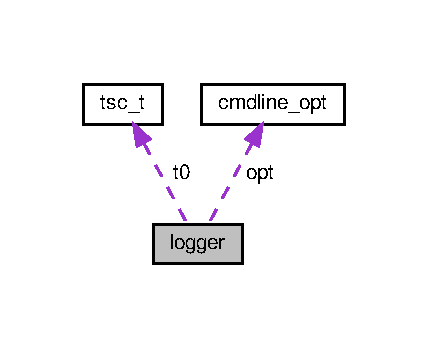
\includegraphics[width=206pt]{structlogger__coll__graph}
\end{center}
\end{figure}
\subsection*{Public Member Functions}
\begin{DoxyCompactItemize}
\item 
\mbox{\Hypertarget{structlogger_afa0e701e9585188b9efa9b547f1120a4}\label{structlogger_afa0e701e9585188b9efa9b547f1120a4}} 
char $\ast$ \hyperlink{structlogger_afa0e701e9585188b9efa9b547f1120a4}{cur\+\_\+time\+\_\+str} ()
\begin{DoxyCompactList}\small\item\em return the current time string like \char`\"{}\+Wed Jun 30 21\+:49\+:08 1993\char`\"{} \end{DoxyCompactList}\item 
int \hyperlink{structlogger_aa079e325d6f0279f803843acc2a8c6f5}{log} (int level, const char $\ast$format,...)
\begin{DoxyCompactList}\small\item\em write a formatted string to the log and may be to standard out \end{DoxyCompactList}\item 
int \hyperlink{structlogger_a2d852f1f257849e0abed587814446908}{start\+\_\+log} (\hyperlink{structcmdline__opt}{cmdline\+\_\+opt} \hyperlink{structlogger_a0e07e1e52c554084e6c3c06476024b9a}{opt})
\begin{DoxyCompactList}\small\item\em open a log file and start logging \end{DoxyCompactList}\item 
\mbox{\Hypertarget{structlogger_ae79e87e0de219c9e001417f5b220c325}\label{structlogger_ae79e87e0de219c9e001417f5b220c325}} 
int \hyperlink{structlogger_ae79e87e0de219c9e001417f5b220c325}{end\+\_\+log} ()
\begin{DoxyCompactList}\small\item\em end logging and close the log file \end{DoxyCompactList}\item 
\mbox{\Hypertarget{structlogger_ac47293937a4c2f844bddf3cc781fab1e}\label{structlogger_ac47293937a4c2f844bddf3cc781fab1e}} 
int \hyperlink{structlogger_ac47293937a4c2f844bddf3cc781fab1e}{log\+\_\+opt} ()
\begin{DoxyCompactList}\small\item\em log command line options to the log file for the record \end{DoxyCompactList}\item 
\mbox{\Hypertarget{structlogger_adbbd2917da3496e2e6e04cf17e115133}\label{structlogger_adbbd2917da3496e2e6e04cf17e115133}} 
int \hyperlink{structlogger_adbbd2917da3496e2e6e04cf17e115133}{log\+\_\+host} ()
\begin{DoxyCompactList}\small\item\em log hostname for the record \end{DoxyCompactList}\item 
\mbox{\Hypertarget{structlogger_a834bbdabbff2c05c342bf3641d6c3966}\label{structlogger_a834bbdabbff2c05c342bf3641d6c3966}} 
int \hyperlink{structlogger_a834bbdabbff2c05c342bf3641d6c3966}{log\+\_\+env} (const char $\ast$var)
\begin{DoxyCompactList}\small\item\em log an environment var for the record \end{DoxyCompactList}\item 
\mbox{\Hypertarget{structlogger_a4de3a6b8949b4155ca57386fd83e1692}\label{structlogger_a4de3a6b8949b4155ca57386fd83e1692}} 
int \hyperlink{structlogger_a4de3a6b8949b4155ca57386fd83e1692}{log\+\_\+envs} ()
\begin{DoxyCompactList}\small\item\em log some environment vars for the record \end{DoxyCompactList}\item 
\mbox{\Hypertarget{structlogger_a88e0dc6e649e35549010eaad9ee713b4}\label{structlogger_a88e0dc6e649e35549010eaad9ee713b4}} 
void \hyperlink{structlogger_a88e0dc6e649e35549010eaad9ee713b4}{log\+\_\+start\+\_\+fun\+\_\+} (const char $\ast$f)
\begin{DoxyCompactList}\small\item\em log the start of a function (f) \end{DoxyCompactList}\item 
\mbox{\Hypertarget{structlogger_a91bda1816b1ceabe5c54184239932b8f}\label{structlogger_a91bda1816b1ceabe5c54184239932b8f}} 
void \hyperlink{structlogger_a91bda1816b1ceabe5c54184239932b8f}{log\+\_\+end\+\_\+fun\+\_\+} (const char $\ast$f, \hyperlink{structtsc__t}{tsc\+\_\+t} \hyperlink{structlogger_a6336fd3fffff10df04811a819c1c5a70}{t0}, \hyperlink{structtsc__t}{tsc\+\_\+t} t1)
\begin{DoxyCompactList}\small\item\em log the end of a function (f) \end{DoxyCompactList}\end{DoxyCompactItemize}
\subsection*{Public Attributes}
\begin{DoxyCompactItemize}
\item 
\hyperlink{structcmdline__opt}{cmdline\+\_\+opt} \hyperlink{structlogger_a0e07e1e52c554084e6c3c06476024b9a}{opt}
\item 
F\+I\+LE $\ast$ \hyperlink{structlogger_ab891d941fb5846a3f8678f1db11c0da9}{log\+\_\+fp}
\item 
\hyperlink{structtsc__t}{tsc\+\_\+t} \hyperlink{structlogger_a6336fd3fffff10df04811a819c1c5a70}{t0}
\end{DoxyCompactItemize}


\subsection{Detailed Description}
logging object 

\subsection{Member Function Documentation}
\mbox{\Hypertarget{structlogger_aa079e325d6f0279f803843acc2a8c6f5}\label{structlogger_aa079e325d6f0279f803843acc2a8c6f5}} 
\index{logger@{logger}!log@{log}}
\index{log@{log}!logger@{logger}}
\subsubsection{\texorpdfstring{log()}{log()}}
{\footnotesize\ttfamily int logger\+::log (\begin{DoxyParamCaption}\item[{int}]{level,  }\item[{const char $\ast$}]{format,  }\item[{}]{... }\end{DoxyParamCaption})\hspace{0.3cm}{\ttfamily [inline]}}



write a formatted string to the log and may be to standard out 


\begin{DoxyParams}{Parameters}
{\em (level)} & the level of this entry. if opt.\+verbose$>$=level, then the string will be output to the standard out (in addition to the log file) \\
\hline
{\em (format)} & the printf-\/like format string \\
\hline
\end{DoxyParams}
\mbox{\Hypertarget{structlogger_a2d852f1f257849e0abed587814446908}\label{structlogger_a2d852f1f257849e0abed587814446908}} 
\index{logger@{logger}!start\+\_\+log@{start\+\_\+log}}
\index{start\+\_\+log@{start\+\_\+log}!logger@{logger}}
\subsubsection{\texorpdfstring{start\+\_\+log()}{start\_log()}}
{\footnotesize\ttfamily int logger\+::start\+\_\+log (\begin{DoxyParamCaption}\item[{\hyperlink{structcmdline__opt}{cmdline\+\_\+opt}}]{opt }\end{DoxyParamCaption})\hspace{0.3cm}{\ttfamily [inline]}}



open a log file and start logging 


\begin{DoxyParams}{Parameters}
{\em (opt)} & command line option \\
\hline
\end{DoxyParams}


\subsection{Member Data Documentation}
\mbox{\Hypertarget{structlogger_ab891d941fb5846a3f8678f1db11c0da9}\label{structlogger_ab891d941fb5846a3f8678f1db11c0da9}} 
\index{logger@{logger}!log\+\_\+fp@{log\+\_\+fp}}
\index{log\+\_\+fp@{log\+\_\+fp}!logger@{logger}}
\subsubsection{\texorpdfstring{log\+\_\+fp}{log\_fp}}
{\footnotesize\ttfamily F\+I\+LE$\ast$ logger\+::log\+\_\+fp}

log file object \mbox{\Hypertarget{structlogger_a0e07e1e52c554084e6c3c06476024b9a}\label{structlogger_a0e07e1e52c554084e6c3c06476024b9a}} 
\index{logger@{logger}!opt@{opt}}
\index{opt@{opt}!logger@{logger}}
\subsubsection{\texorpdfstring{opt}{opt}}
{\footnotesize\ttfamily \hyperlink{structcmdline__opt}{cmdline\+\_\+opt} logger\+::opt}

command line options \mbox{\Hypertarget{structlogger_a6336fd3fffff10df04811a819c1c5a70}\label{structlogger_a6336fd3fffff10df04811a819c1c5a70}} 
\index{logger@{logger}!t0@{t0}}
\index{t0@{t0}!logger@{logger}}
\subsubsection{\texorpdfstring{t0}{t0}}
{\footnotesize\ttfamily \hyperlink{structtsc__t}{tsc\+\_\+t} logger\+::t0}

the start time stamp 

The documentation for this struct was generated from the following file\+:\begin{DoxyCompactItemize}
\item 
/home/tau/public\+\_\+html/lecture/parallel\+\_\+distributed/2018/handson/tau/parallel-\/distributed-\/handson/20vgg/include/\hyperlink{vgg__util_8h}{vgg\+\_\+util.\+h}\end{DoxyCompactItemize}

\hypertarget{structMaxPooling2D}{}\section{Max\+Pooling2D$<$ maxB, C, H, W, S $>$ Struct Template Reference}
\label{structMaxPooling2D}\index{Max\+Pooling2\+D$<$ max\+B, C, H, W, S $>$@{Max\+Pooling2\+D$<$ max\+B, C, H, W, S $>$}}


max pooling layer  




{\ttfamily \#include $<$maxpooling.\+h$>$}



Collaboration diagram for Max\+Pooling2D$<$ maxB, C, H, W, S $>$\+:\nopagebreak
\begin{figure}[H]
\begin{center}
\leavevmode
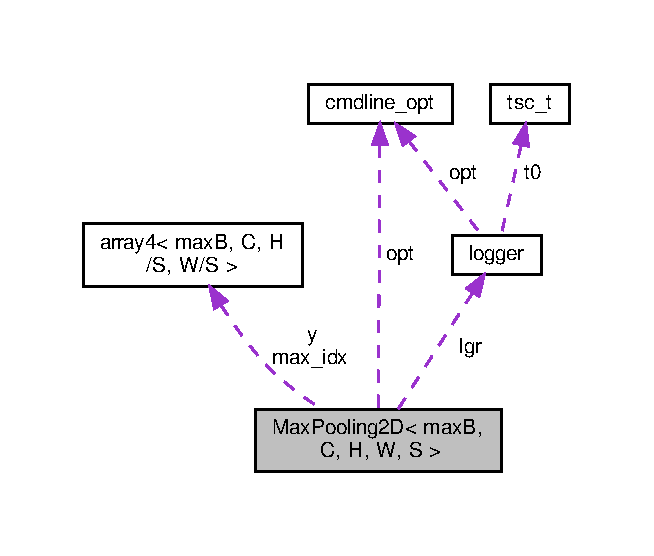
\includegraphics[width=314pt]{structMaxPooling2D__coll__graph}
\end{center}
\end{figure}
\subsection*{Public Member Functions}
\begin{DoxyCompactItemize}
\item 
void \hyperlink{structMaxPooling2D_a004da9768f6934b82ce6758ab7da92be}{init} (\hyperlink{structcmdline__opt}{cmdline\+\_\+opt} \hyperlink{structMaxPooling2D_a573bf3df3ae3d9043763c6743f1b87f9}{opt}, \hyperlink{structlogger}{logger} $\ast$\hyperlink{structMaxPooling2D_a516ea469a544d99543c9073bc318f970}{lgr})
\begin{DoxyCompactList}\small\item\em initialize \end{DoxyCompactList}\item 
\hyperlink{structMaxPooling2D}{Max\+Pooling2D}$<$ maxB, C, H, W, S $>$ $\ast$ \hyperlink{structMaxPooling2D_a84452150daaa577f3a13d13e429d1eca}{copy} ()
\begin{DoxyCompactList}\small\item\em make a copy of this \end{DoxyCompactList}\item 
void \hyperlink{structMaxPooling2D_ab534c745a6fbfac5a8bd1718a1510dbe}{set\+\_\+dev} (\hyperlink{structMaxPooling2D}{Max\+Pooling2D}$<$ maxB, C, H, W, S $>$ $\ast$\hyperlink{structMaxPooling2D_ad21014604fa6abddbfdcdc0b64f37196}{dev})
\begin{DoxyCompactList}\small\item\em set the device pointer for this and all subobjects \end{DoxyCompactList}\item 
void \hyperlink{structMaxPooling2D_a2cb8392bfcf78dc55e7157ef3095364e}{make\+\_\+dev} ()
\begin{DoxyCompactList}\small\item\em if the algorithm is a gpu algorithm, allocate a device shadow of this object and set dev field of this and all subobjects. otherwise it sets all dev fields to null. \end{DoxyCompactList}\item 
void \hyperlink{structMaxPooling2D_a5d3cd9d8a476ae96cb7f86b5a0409f72}{del\+\_\+dev} ()
\begin{DoxyCompactList}\small\item\em if the algorithm is a gpu algorithm, dev field must not be null and deallocate it. \end{DoxyCompactList}\item 
\mbox{\Hypertarget{structMaxPooling2D_ab99bc63b1e21dc7839b05d4ef299d9fd}\label{structMaxPooling2D_ab99bc63b1e21dc7839b05d4ef299d9fd}} 
void \hyperlink{structMaxPooling2D_ab99bc63b1e21dc7839b05d4ef299d9fd}{to\+\_\+dev} ()
\begin{DoxyCompactList}\small\item\em if the algorithm is a gpu algorithm, dev field must not be null and send the host data to the device memory \end{DoxyCompactList}\item 
\mbox{\Hypertarget{structMaxPooling2D_a457aa9a435b46cbf6419aa91d5a8a007}\label{structMaxPooling2D_a457aa9a435b46cbf6419aa91d5a8a007}} 
void \hyperlink{structMaxPooling2D_a457aa9a435b46cbf6419aa91d5a8a007}{to\+\_\+host} ()
\begin{DoxyCompactList}\small\item\em if the algorithm is a gpu algorithm, dev field must not be null and send the device data to the host memory \end{DoxyCompactList}\item 
\+\_\+\+\_\+device\+\_\+\+\_\+ \+\_\+\+\_\+host\+\_\+\+\_\+ void \hyperlink{structMaxPooling2D_adde941f72d6c91ecb63253afb845dbfa}{forward\+\_\+base} (\hyperlink{structarray4}{array4}$<$ maxB, C, H, W $>$ \&x)
\begin{DoxyCompactList}\small\item\em the baseline (serial) implementation of forward called both by cpu implementation (forward\+\_\+cpu) and gpu implementation (forward\+\_\+dev). the call sequence forward -\/$>$ forward\+\_\+cpu -\/$>$ forward\+\_\+base on cpu and and is forward -\/$>$ forward\+\_\+gpu -\/$>$ forward\+\_\+global -\/$>$ forward\+\_\+dev -\/$>$ forward\+\_\+base \end{DoxyCompactList}\item 
\+\_\+\+\_\+device\+\_\+\+\_\+ void \hyperlink{structMaxPooling2D_a978800c6648a820257f2934e9970e12e}{forward\+\_\+dev} (\hyperlink{structarray4}{array4}$<$ maxB, C, H, W $>$ \&x)
\begin{DoxyCompactList}\small\item\em the device function of forward called from the global (non-\/member) function \end{DoxyCompactList}\item 
void \hyperlink{structMaxPooling2D_a4e8ee0e7bf1cc0b7688fbbe1b04019ec}{forward\+\_\+gpu} (\hyperlink{structarray4}{array4}$<$ maxB, C, H, W $>$ \&x)
\begin{DoxyCompactList}\small\item\em a gpu version of baseline code called from the entry function (forward) \end{DoxyCompactList}\item 
void \hyperlink{structMaxPooling2D_a3f9af927ce1e269b42c097bdb64ef90a}{forward\+\_\+cpu} (\hyperlink{structarray4}{array4}$<$ maxB, C, H, W $>$ \&x)
\begin{DoxyCompactList}\small\item\em a cpu version of baseline code called from the entry function (forward) \end{DoxyCompactList}\item 
\hyperlink{structarray4}{array4}$<$ maxB, C, H/S, W/S $>$ \& \hyperlink{structMaxPooling2D_ac533b4e08d8f2e708bbdc8f8e2d784a2}{forward} (\hyperlink{structarray4}{array4}$<$ maxB, C, H, W $>$ \&x)
\begin{DoxyCompactList}\small\item\em calc the loss function of a mini-\/batch (x) \end{DoxyCompactList}\item 
\+\_\+\+\_\+device\+\_\+\+\_\+ \+\_\+\+\_\+host\+\_\+\+\_\+ void \hyperlink{structMaxPooling2D_a3a2ce37cba46cc7cfd219e55bb3c2f29}{backward\+\_\+base} (\hyperlink{structarray4}{array4}$<$ maxB, C, H/S, W/S $>$ \&gy)
\begin{DoxyCompactList}\small\item\em the baseline (serial) implementation of backward called both by cpu implementation (backward\+\_\+cpu) and gpu implementation (backward\+\_\+dev). the call sequence backward -\/$>$ backward\+\_\+cpu -\/$>$ backward\+\_\+base on cpu and and is backward -\/$>$ backward\+\_\+gpu -\/$>$ backward\+\_\+global -\/$>$ backward\+\_\+dev -\/$>$ backward\+\_\+base \end{DoxyCompactList}\item 
\+\_\+\+\_\+device\+\_\+\+\_\+ void \hyperlink{structMaxPooling2D_ad54e972c24822a97aac4f43066d25db8}{backward\+\_\+dev} (\hyperlink{structarray4}{array4}$<$ maxB, C, H/S, W/S $>$ \&gy)
\begin{DoxyCompactList}\small\item\em the device function of backward called from the global (non-\/member) function \end{DoxyCompactList}\item 
void \hyperlink{structMaxPooling2D_ae7d3c7c84e64b9060471973b58899315}{backward\+\_\+gpu} (\hyperlink{structarray4}{array4}$<$ maxB, C, H/S, W/S $>$ \&gy)
\begin{DoxyCompactList}\small\item\em a gpu version of baseline code called from the entry function (backward) \end{DoxyCompactList}\item 
void \hyperlink{structMaxPooling2D_a28487a560998c1eb511f3d4e3b948fd6}{backward\+\_\+cpu} (\hyperlink{structarray4}{array4}$<$ maxB, C, H/S, W/S $>$ \&gy)
\begin{DoxyCompactList}\small\item\em a cpu version of baseline code called from the entry function (backward) \end{DoxyCompactList}\item 
\hyperlink{structarray4}{array4}$<$ maxB, C, H, W $>$ \& \hyperlink{structMaxPooling2D_ae0ad0f868dcf5f976f4dd99dd91e2f91}{backward} (\hyperlink{structarray4}{array4}$<$ maxB, C, H/S, W/S $>$ \&gy)
\begin{DoxyCompactList}\small\item\em calc the gradient of loss wrt the input (x) \end{DoxyCompactList}\end{DoxyCompactItemize}
\subsection*{Public Attributes}
\begin{DoxyCompactItemize}
\item 
\hyperlink{structMaxPooling2D}{Max\+Pooling2D}$<$ maxB, C, H, W, S $>$ $\ast$ \hyperlink{structMaxPooling2D_ad21014604fa6abddbfdcdc0b64f37196}{dev}
\item 
\hyperlink{structcmdline__opt}{cmdline\+\_\+opt} \hyperlink{structMaxPooling2D_a573bf3df3ae3d9043763c6743f1b87f9}{opt}
\item 
\hyperlink{structlogger}{logger} $\ast$ \hyperlink{structMaxPooling2D_a516ea469a544d99543c9073bc318f970}{lgr}
\item 
\hyperlink{structarray4}{array4}$<$ maxB, C, H/S, W/S $>$ \hyperlink{structMaxPooling2D_a0ad5375e31a495c53600f3367da9fddc}{y}
\item 
\hyperlink{structarray4}{array4}$<$ maxB, C, H/S, W/S $>$ \hyperlink{structMaxPooling2D_ac6ca7dc8ceca1e9e5d2403634ebd8802}{max\+\_\+idx}
\item 
\hyperlink{structarray4}{array4}$<$ maxB, C, H, W $>$ \hyperlink{structMaxPooling2D_abf5754c5b154e54b09c38bc2c189562b}{gx}
\end{DoxyCompactItemize}


\subsection{Detailed Description}
\subsubsection*{template$<$idx\+\_\+t maxB, idx\+\_\+t C, idx\+\_\+t H, idx\+\_\+t W, idx\+\_\+t S$>$\newline
struct Max\+Pooling2\+D$<$ max\+B, C, H, W, S $>$}

max pooling layer 


\begin{DoxyParams}{Parameters}
{\em (max\+B)} & the maximum number of images (batch size) \\
\hline
{\em (\+C)} & the number of channels per input image (the original input has typically three channels for R\+GB. in hidden layers, it starts from 64 and goes up to 512 in the last hidden layer) \\
\hline
{\em (\+H)} & height of an image (32 for an input image, down to 1 in the last hidden layer) \\
\hline
{\em (\+W)} & width of an image (32 for an input image, down to 1 in the last hidden layer) \\
\hline
{\em (\+S)} & shrink factor of pooling layers (2)\\
\hline
\end{DoxyParams}
this layer implements max pooling. it takes SxS patch of input images and take the maximum of it. given an HxW image, output (H/S)x(W/S) image 

\subsection{Member Function Documentation}
\mbox{\Hypertarget{structMaxPooling2D_ae0ad0f868dcf5f976f4dd99dd91e2f91}\label{structMaxPooling2D_ae0ad0f868dcf5f976f4dd99dd91e2f91}} 
\index{Max\+Pooling2D@{Max\+Pooling2D}!backward@{backward}}
\index{backward@{backward}!Max\+Pooling2D@{Max\+Pooling2D}}
\subsubsection{\texorpdfstring{backward()}{backward()}}
{\footnotesize\ttfamily template$<$idx\+\_\+t maxB, idx\+\_\+t C, idx\+\_\+t H, idx\+\_\+t W, idx\+\_\+t S$>$ \\
\hyperlink{structarray4}{array4}$<$maxB,C,H,W$>$\& \hyperlink{structMaxPooling2D}{Max\+Pooling2D}$<$ maxB, C, H, W, S $>$\+::backward (\begin{DoxyParamCaption}\item[{\hyperlink{structarray4}{array4}$<$ maxB, C, H/S, W/S $>$ \&}]{gy }\end{DoxyParamCaption})\hspace{0.3cm}{\ttfamily [inline]}}



calc the gradient of loss wrt the input (x) 


\begin{DoxyParams}{Parameters}
{\em (gy)} & gradient of loss with respect to the output\\
\hline
\end{DoxyParams}
calc the gradient of loss wrt the input. along the way, it also calculates the gradient of loss wrt weights for all sublayers that have weights. since this is the entire network, gy is actually a vector whose components are all 1. (loss = sum of losses of each data). \begin{DoxySeeAlso}{See also}
\hyperlink{structMaxPooling2D_ac533b4e08d8f2e708bbdc8f8e2d784a2}{forward} 

update 
\end{DoxySeeAlso}
\mbox{\Hypertarget{structMaxPooling2D_a3a2ce37cba46cc7cfd219e55bb3c2f29}\label{structMaxPooling2D_a3a2ce37cba46cc7cfd219e55bb3c2f29}} 
\index{Max\+Pooling2D@{Max\+Pooling2D}!backward\+\_\+base@{backward\+\_\+base}}
\index{backward\+\_\+base@{backward\+\_\+base}!Max\+Pooling2D@{Max\+Pooling2D}}
\subsubsection{\texorpdfstring{backward\+\_\+base()}{backward\_base()}}
{\footnotesize\ttfamily template$<$idx\+\_\+t maxB, idx\+\_\+t C, idx\+\_\+t H, idx\+\_\+t W, idx\+\_\+t S$>$ \\
\+\_\+\+\_\+device\+\_\+\+\_\+ \+\_\+\+\_\+host\+\_\+\+\_\+ void \hyperlink{structMaxPooling2D}{Max\+Pooling2D}$<$ maxB, C, H, W, S $>$\+::backward\+\_\+base (\begin{DoxyParamCaption}\item[{\hyperlink{structarray4}{array4}$<$ maxB, C, H/S, W/S $>$ \&}]{gy }\end{DoxyParamCaption})\hspace{0.3cm}{\ttfamily [inline]}}



the baseline (serial) implementation of backward called both by cpu implementation (backward\+\_\+cpu) and gpu implementation (backward\+\_\+dev). the call sequence backward -\/$>$ backward\+\_\+cpu -\/$>$ backward\+\_\+base on cpu and and is backward -\/$>$ backward\+\_\+gpu -\/$>$ backward\+\_\+global -\/$>$ backward\+\_\+dev -\/$>$ backward\+\_\+base 


\begin{DoxyParams}{Parameters}
{\em (gy)} & gradient of loss with respect to the output \\
\hline
\end{DoxyParams}
\begin{DoxySeeAlso}{See also}
\hyperlink{structMaxPooling2D_ae0ad0f868dcf5f976f4dd99dd91e2f91}{backward} 

\hyperlink{structMaxPooling2D_ae7d3c7c84e64b9060471973b58899315}{backward\+\_\+gpu} 

\hyperlink{softmaxcrossentropy_8h_a47d56a9a23e08247b227f4aac17413e0}{backward\+\_\+global} 

\hyperlink{structMaxPooling2D_ad54e972c24822a97aac4f43066d25db8}{backward\+\_\+dev} 
\end{DoxySeeAlso}
\mbox{\Hypertarget{structMaxPooling2D_a28487a560998c1eb511f3d4e3b948fd6}\label{structMaxPooling2D_a28487a560998c1eb511f3d4e3b948fd6}} 
\index{Max\+Pooling2D@{Max\+Pooling2D}!backward\+\_\+cpu@{backward\+\_\+cpu}}
\index{backward\+\_\+cpu@{backward\+\_\+cpu}!Max\+Pooling2D@{Max\+Pooling2D}}
\subsubsection{\texorpdfstring{backward\+\_\+cpu()}{backward\_cpu()}}
{\footnotesize\ttfamily template$<$idx\+\_\+t maxB, idx\+\_\+t C, idx\+\_\+t H, idx\+\_\+t W, idx\+\_\+t S$>$ \\
void \hyperlink{structMaxPooling2D}{Max\+Pooling2D}$<$ maxB, C, H, W, S $>$\+::backward\+\_\+cpu (\begin{DoxyParamCaption}\item[{\hyperlink{structarray4}{array4}$<$ maxB, C, H/S, W/S $>$ \&}]{gy }\end{DoxyParamCaption})\hspace{0.3cm}{\ttfamily [inline]}}



a cpu version of baseline code called from the entry function (backward) 


\begin{DoxyParams}{Parameters}
{\em (gy)} & gradient of loss with respect to the output \\
\hline
\end{DoxyParams}
\begin{DoxySeeAlso}{See also}
\hyperlink{structMaxPooling2D_ae0ad0f868dcf5f976f4dd99dd91e2f91}{backward} 

\hyperlink{structMaxPooling2D_a3a2ce37cba46cc7cfd219e55bb3c2f29}{backward\+\_\+base} 
\end{DoxySeeAlso}
\mbox{\Hypertarget{structMaxPooling2D_ad54e972c24822a97aac4f43066d25db8}\label{structMaxPooling2D_ad54e972c24822a97aac4f43066d25db8}} 
\index{Max\+Pooling2D@{Max\+Pooling2D}!backward\+\_\+dev@{backward\+\_\+dev}}
\index{backward\+\_\+dev@{backward\+\_\+dev}!Max\+Pooling2D@{Max\+Pooling2D}}
\subsubsection{\texorpdfstring{backward\+\_\+dev()}{backward\_dev()}}
{\footnotesize\ttfamily template$<$idx\+\_\+t maxB, idx\+\_\+t C, idx\+\_\+t H, idx\+\_\+t W, idx\+\_\+t S$>$ \\
\+\_\+\+\_\+device\+\_\+\+\_\+ void \hyperlink{structMaxPooling2D}{Max\+Pooling2D}$<$ maxB, C, H, W, S $>$\+::backward\+\_\+dev (\begin{DoxyParamCaption}\item[{\hyperlink{structarray4}{array4}$<$ maxB, C, H/S, W/S $>$ \&}]{gy }\end{DoxyParamCaption})\hspace{0.3cm}{\ttfamily [inline]}}



the device function of backward called from the global (non-\/member) function 


\begin{DoxyParams}{Parameters}
{\em (gy)} & gradient of loss with respect to the output \\
\hline
\end{DoxyParams}
\begin{DoxySeeAlso}{See also}
\hyperlink{structMaxPooling2D_ae0ad0f868dcf5f976f4dd99dd91e2f91}{backward} 

\hyperlink{structMaxPooling2D_ae7d3c7c84e64b9060471973b58899315}{backward\+\_\+gpu} 

\hyperlink{softmaxcrossentropy_8h_a47d56a9a23e08247b227f4aac17413e0}{backward\+\_\+global} 

\hyperlink{structMaxPooling2D_a3a2ce37cba46cc7cfd219e55bb3c2f29}{backward\+\_\+base} 
\end{DoxySeeAlso}
\mbox{\Hypertarget{structMaxPooling2D_ae7d3c7c84e64b9060471973b58899315}\label{structMaxPooling2D_ae7d3c7c84e64b9060471973b58899315}} 
\index{Max\+Pooling2D@{Max\+Pooling2D}!backward\+\_\+gpu@{backward\+\_\+gpu}}
\index{backward\+\_\+gpu@{backward\+\_\+gpu}!Max\+Pooling2D@{Max\+Pooling2D}}
\subsubsection{\texorpdfstring{backward\+\_\+gpu()}{backward\_gpu()}}
{\footnotesize\ttfamily template$<$idx\+\_\+t maxB, idx\+\_\+t C, idx\+\_\+t H, idx\+\_\+t W, idx\+\_\+t S$>$ \\
void \hyperlink{structMaxPooling2D}{Max\+Pooling2D}$<$ maxB, C, H, W, S $>$\+::backward\+\_\+gpu (\begin{DoxyParamCaption}\item[{\hyperlink{structarray4}{array4}$<$ maxB, C, H/S, W/S $>$ \&}]{gy }\end{DoxyParamCaption})\hspace{0.3cm}{\ttfamily [inline]}}



a gpu version of baseline code called from the entry function (backward) 


\begin{DoxyParams}{Parameters}
{\em (gy)} & gradient of loss with respect to the output \\
\hline
\end{DoxyParams}
\begin{DoxySeeAlso}{See also}
\hyperlink{structMaxPooling2D_ae0ad0f868dcf5f976f4dd99dd91e2f91}{backward} 

\hyperlink{softmaxcrossentropy_8h_a47d56a9a23e08247b227f4aac17413e0}{backward\+\_\+global} 

\hyperlink{structMaxPooling2D_ad54e972c24822a97aac4f43066d25db8}{backward\+\_\+dev} 

\hyperlink{structMaxPooling2D_a3a2ce37cba46cc7cfd219e55bb3c2f29}{backward\+\_\+base} 
\end{DoxySeeAlso}
\mbox{\Hypertarget{structMaxPooling2D_a84452150daaa577f3a13d13e429d1eca}\label{structMaxPooling2D_a84452150daaa577f3a13d13e429d1eca}} 
\index{Max\+Pooling2D@{Max\+Pooling2D}!copy@{copy}}
\index{copy@{copy}!Max\+Pooling2D@{Max\+Pooling2D}}
\subsubsection{\texorpdfstring{copy()}{copy()}}
{\footnotesize\ttfamily template$<$idx\+\_\+t maxB, idx\+\_\+t C, idx\+\_\+t H, idx\+\_\+t W, idx\+\_\+t S$>$ \\
\hyperlink{structMaxPooling2D}{Max\+Pooling2D}$<$maxB,C,H,W,S$>$$\ast$ \hyperlink{structMaxPooling2D}{Max\+Pooling2D}$<$ maxB, C, H, W, S $>$\+::copy (\begin{DoxyParamCaption}{ }\end{DoxyParamCaption})\hspace{0.3cm}{\ttfamily [inline]}}



make a copy of this 

if this object has a device pointer, the copy will have a device pointer too, but its contents are N\+OT copied \mbox{\Hypertarget{structMaxPooling2D_a5d3cd9d8a476ae96cb7f86b5a0409f72}\label{structMaxPooling2D_a5d3cd9d8a476ae96cb7f86b5a0409f72}} 
\index{Max\+Pooling2D@{Max\+Pooling2D}!del\+\_\+dev@{del\+\_\+dev}}
\index{del\+\_\+dev@{del\+\_\+dev}!Max\+Pooling2D@{Max\+Pooling2D}}
\subsubsection{\texorpdfstring{del\+\_\+dev()}{del\_dev()}}
{\footnotesize\ttfamily template$<$idx\+\_\+t maxB, idx\+\_\+t C, idx\+\_\+t H, idx\+\_\+t W, idx\+\_\+t S$>$ \\
void \hyperlink{structMaxPooling2D}{Max\+Pooling2D}$<$ maxB, C, H, W, S $>$\+::del\+\_\+dev (\begin{DoxyParamCaption}{ }\end{DoxyParamCaption})\hspace{0.3cm}{\ttfamily [inline]}}



if the algorithm is a gpu algorithm, dev field must not be null and deallocate it. 

\begin{DoxySeeAlso}{See also}
\hyperlink{structMaxPooling2D_a2cb8392bfcf78dc55e7157ef3095364e}{make\+\_\+dev} 

\hyperlink{structMaxPooling2D_ab534c745a6fbfac5a8bd1718a1510dbe}{set\+\_\+dev} 
\end{DoxySeeAlso}
\mbox{\Hypertarget{structMaxPooling2D_ac533b4e08d8f2e708bbdc8f8e2d784a2}\label{structMaxPooling2D_ac533b4e08d8f2e708bbdc8f8e2d784a2}} 
\index{Max\+Pooling2D@{Max\+Pooling2D}!forward@{forward}}
\index{forward@{forward}!Max\+Pooling2D@{Max\+Pooling2D}}
\subsubsection{\texorpdfstring{forward()}{forward()}}
{\footnotesize\ttfamily template$<$idx\+\_\+t maxB, idx\+\_\+t C, idx\+\_\+t H, idx\+\_\+t W, idx\+\_\+t S$>$ \\
\hyperlink{structarray4}{array4}$<$maxB,C,H/S,W/S$>$\& \hyperlink{structMaxPooling2D}{Max\+Pooling2D}$<$ maxB, C, H, W, S $>$\+::forward (\begin{DoxyParamCaption}\item[{\hyperlink{structarray4}{array4}$<$ maxB, C, H, W $>$ \&}]{x }\end{DoxyParamCaption})\hspace{0.3cm}{\ttfamily [inline]}}



calc the loss function of a mini-\/batch (x) 


\begin{DoxyParams}{Parameters}
{\em (x)} & input images \\
\hline
\end{DoxyParams}
\begin{DoxySeeAlso}{See also}
\hyperlink{structMaxPooling2D_ae0ad0f868dcf5f976f4dd99dd91e2f91}{backward} 

update 
\end{DoxySeeAlso}
\mbox{\Hypertarget{structMaxPooling2D_adde941f72d6c91ecb63253afb845dbfa}\label{structMaxPooling2D_adde941f72d6c91ecb63253afb845dbfa}} 
\index{Max\+Pooling2D@{Max\+Pooling2D}!forward\+\_\+base@{forward\+\_\+base}}
\index{forward\+\_\+base@{forward\+\_\+base}!Max\+Pooling2D@{Max\+Pooling2D}}
\subsubsection{\texorpdfstring{forward\+\_\+base()}{forward\_base()}}
{\footnotesize\ttfamily template$<$idx\+\_\+t maxB, idx\+\_\+t C, idx\+\_\+t H, idx\+\_\+t W, idx\+\_\+t S$>$ \\
\+\_\+\+\_\+device\+\_\+\+\_\+ \+\_\+\+\_\+host\+\_\+\+\_\+ void \hyperlink{structMaxPooling2D}{Max\+Pooling2D}$<$ maxB, C, H, W, S $>$\+::forward\+\_\+base (\begin{DoxyParamCaption}\item[{\hyperlink{structarray4}{array4}$<$ maxB, C, H, W $>$ \&}]{x }\end{DoxyParamCaption})\hspace{0.3cm}{\ttfamily [inline]}}



the baseline (serial) implementation of forward called both by cpu implementation (forward\+\_\+cpu) and gpu implementation (forward\+\_\+dev). the call sequence forward -\/$>$ forward\+\_\+cpu -\/$>$ forward\+\_\+base on cpu and and is forward -\/$>$ forward\+\_\+gpu -\/$>$ forward\+\_\+global -\/$>$ forward\+\_\+dev -\/$>$ forward\+\_\+base 


\begin{DoxyParams}{Parameters}
{\em (x)} & input images \\
\hline
\end{DoxyParams}
\begin{DoxySeeAlso}{See also}
\hyperlink{structMaxPooling2D_ac533b4e08d8f2e708bbdc8f8e2d784a2}{forward} 

\hyperlink{structMaxPooling2D_a4e8ee0e7bf1cc0b7688fbbe1b04019ec}{forward\+\_\+gpu} 

\hyperlink{softmaxcrossentropy_8h_a578aeeb166bd06e800d9b396eab48b35}{forward\+\_\+global} 

\hyperlink{structMaxPooling2D_a978800c6648a820257f2934e9970e12e}{forward\+\_\+dev} 
\end{DoxySeeAlso}
\mbox{\Hypertarget{structMaxPooling2D_a3f9af927ce1e269b42c097bdb64ef90a}\label{structMaxPooling2D_a3f9af927ce1e269b42c097bdb64ef90a}} 
\index{Max\+Pooling2D@{Max\+Pooling2D}!forward\+\_\+cpu@{forward\+\_\+cpu}}
\index{forward\+\_\+cpu@{forward\+\_\+cpu}!Max\+Pooling2D@{Max\+Pooling2D}}
\subsubsection{\texorpdfstring{forward\+\_\+cpu()}{forward\_cpu()}}
{\footnotesize\ttfamily template$<$idx\+\_\+t maxB, idx\+\_\+t C, idx\+\_\+t H, idx\+\_\+t W, idx\+\_\+t S$>$ \\
void \hyperlink{structMaxPooling2D}{Max\+Pooling2D}$<$ maxB, C, H, W, S $>$\+::forward\+\_\+cpu (\begin{DoxyParamCaption}\item[{\hyperlink{structarray4}{array4}$<$ maxB, C, H, W $>$ \&}]{x }\end{DoxyParamCaption})\hspace{0.3cm}{\ttfamily [inline]}}



a cpu version of baseline code called from the entry function (forward) 


\begin{DoxyParams}{Parameters}
{\em (x)} & input images \\
\hline
\end{DoxyParams}
\begin{DoxySeeAlso}{See also}
\hyperlink{structMaxPooling2D_ac533b4e08d8f2e708bbdc8f8e2d784a2}{forward} 

\hyperlink{structMaxPooling2D_adde941f72d6c91ecb63253afb845dbfa}{forward\+\_\+base} 
\end{DoxySeeAlso}
\mbox{\Hypertarget{structMaxPooling2D_a978800c6648a820257f2934e9970e12e}\label{structMaxPooling2D_a978800c6648a820257f2934e9970e12e}} 
\index{Max\+Pooling2D@{Max\+Pooling2D}!forward\+\_\+dev@{forward\+\_\+dev}}
\index{forward\+\_\+dev@{forward\+\_\+dev}!Max\+Pooling2D@{Max\+Pooling2D}}
\subsubsection{\texorpdfstring{forward\+\_\+dev()}{forward\_dev()}}
{\footnotesize\ttfamily template$<$idx\+\_\+t maxB, idx\+\_\+t C, idx\+\_\+t H, idx\+\_\+t W, idx\+\_\+t S$>$ \\
\+\_\+\+\_\+device\+\_\+\+\_\+ void \hyperlink{structMaxPooling2D}{Max\+Pooling2D}$<$ maxB, C, H, W, S $>$\+::forward\+\_\+dev (\begin{DoxyParamCaption}\item[{\hyperlink{structarray4}{array4}$<$ maxB, C, H, W $>$ \&}]{x }\end{DoxyParamCaption})\hspace{0.3cm}{\ttfamily [inline]}}



the device function of forward called from the global (non-\/member) function 


\begin{DoxyParams}{Parameters}
{\em (x)} & input images \\
\hline
\end{DoxyParams}
\begin{DoxySeeAlso}{See also}
\hyperlink{structMaxPooling2D_ac533b4e08d8f2e708bbdc8f8e2d784a2}{forward} 

\hyperlink{structMaxPooling2D_a4e8ee0e7bf1cc0b7688fbbe1b04019ec}{forward\+\_\+gpu} 

\hyperlink{softmaxcrossentropy_8h_a578aeeb166bd06e800d9b396eab48b35}{forward\+\_\+global} 

\hyperlink{structMaxPooling2D_adde941f72d6c91ecb63253afb845dbfa}{forward\+\_\+base} 
\end{DoxySeeAlso}
\mbox{\Hypertarget{structMaxPooling2D_a4e8ee0e7bf1cc0b7688fbbe1b04019ec}\label{structMaxPooling2D_a4e8ee0e7bf1cc0b7688fbbe1b04019ec}} 
\index{Max\+Pooling2D@{Max\+Pooling2D}!forward\+\_\+gpu@{forward\+\_\+gpu}}
\index{forward\+\_\+gpu@{forward\+\_\+gpu}!Max\+Pooling2D@{Max\+Pooling2D}}
\subsubsection{\texorpdfstring{forward\+\_\+gpu()}{forward\_gpu()}}
{\footnotesize\ttfamily template$<$idx\+\_\+t maxB, idx\+\_\+t C, idx\+\_\+t H, idx\+\_\+t W, idx\+\_\+t S$>$ \\
void \hyperlink{structMaxPooling2D}{Max\+Pooling2D}$<$ maxB, C, H, W, S $>$\+::forward\+\_\+gpu (\begin{DoxyParamCaption}\item[{\hyperlink{structarray4}{array4}$<$ maxB, C, H, W $>$ \&}]{x }\end{DoxyParamCaption})\hspace{0.3cm}{\ttfamily [inline]}}



a gpu version of baseline code called from the entry function (forward) 


\begin{DoxyParams}{Parameters}
{\em (x)} & input images \\
\hline
\end{DoxyParams}
\begin{DoxySeeAlso}{See also}
\hyperlink{structMaxPooling2D_ac533b4e08d8f2e708bbdc8f8e2d784a2}{forward} 

\hyperlink{softmaxcrossentropy_8h_a578aeeb166bd06e800d9b396eab48b35}{forward\+\_\+global} 

\hyperlink{structMaxPooling2D_a978800c6648a820257f2934e9970e12e}{forward\+\_\+dev} 

\hyperlink{structMaxPooling2D_adde941f72d6c91ecb63253afb845dbfa}{forward\+\_\+base} 
\end{DoxySeeAlso}
\mbox{\Hypertarget{structMaxPooling2D_a004da9768f6934b82ce6758ab7da92be}\label{structMaxPooling2D_a004da9768f6934b82ce6758ab7da92be}} 
\index{Max\+Pooling2D@{Max\+Pooling2D}!init@{init}}
\index{init@{init}!Max\+Pooling2D@{Max\+Pooling2D}}
\subsubsection{\texorpdfstring{init()}{init()}}
{\footnotesize\ttfamily template$<$idx\+\_\+t maxB, idx\+\_\+t C, idx\+\_\+t H, idx\+\_\+t W, idx\+\_\+t S$>$ \\
void \hyperlink{structMaxPooling2D}{Max\+Pooling2D}$<$ maxB, C, H, W, S $>$\+::init (\begin{DoxyParamCaption}\item[{\hyperlink{structcmdline__opt}{cmdline\+\_\+opt}}]{opt,  }\item[{\hyperlink{structlogger}{logger} $\ast$}]{lgr }\end{DoxyParamCaption})\hspace{0.3cm}{\ttfamily [inline]}}



initialize 


\begin{DoxyParams}{Parameters}
{\em (opt)} & command line options \\
\hline
{\em (lgr)} & logger \\
\hline
\end{DoxyParams}
\mbox{\Hypertarget{structMaxPooling2D_a2cb8392bfcf78dc55e7157ef3095364e}\label{structMaxPooling2D_a2cb8392bfcf78dc55e7157ef3095364e}} 
\index{Max\+Pooling2D@{Max\+Pooling2D}!make\+\_\+dev@{make\+\_\+dev}}
\index{make\+\_\+dev@{make\+\_\+dev}!Max\+Pooling2D@{Max\+Pooling2D}}
\subsubsection{\texorpdfstring{make\+\_\+dev()}{make\_dev()}}
{\footnotesize\ttfamily template$<$idx\+\_\+t maxB, idx\+\_\+t C, idx\+\_\+t H, idx\+\_\+t W, idx\+\_\+t S$>$ \\
void \hyperlink{structMaxPooling2D}{Max\+Pooling2D}$<$ maxB, C, H, W, S $>$\+::make\+\_\+dev (\begin{DoxyParamCaption}{ }\end{DoxyParamCaption})\hspace{0.3cm}{\ttfamily [inline]}}



if the algorithm is a gpu algorithm, allocate a device shadow of this object and set dev field of this and all subobjects. otherwise it sets all dev fields to null. 

\begin{DoxySeeAlso}{See also}
\hyperlink{structMaxPooling2D_ab534c745a6fbfac5a8bd1718a1510dbe}{set\+\_\+dev} 

\hyperlink{structMaxPooling2D_a5d3cd9d8a476ae96cb7f86b5a0409f72}{del\+\_\+dev} 
\end{DoxySeeAlso}
\mbox{\Hypertarget{structMaxPooling2D_ab534c745a6fbfac5a8bd1718a1510dbe}\label{structMaxPooling2D_ab534c745a6fbfac5a8bd1718a1510dbe}} 
\index{Max\+Pooling2D@{Max\+Pooling2D}!set\+\_\+dev@{set\+\_\+dev}}
\index{set\+\_\+dev@{set\+\_\+dev}!Max\+Pooling2D@{Max\+Pooling2D}}
\subsubsection{\texorpdfstring{set\+\_\+dev()}{set\_dev()}}
{\footnotesize\ttfamily template$<$idx\+\_\+t maxB, idx\+\_\+t C, idx\+\_\+t H, idx\+\_\+t W, idx\+\_\+t S$>$ \\
void \hyperlink{structMaxPooling2D}{Max\+Pooling2D}$<$ maxB, C, H, W, S $>$\+::set\+\_\+dev (\begin{DoxyParamCaption}\item[{\hyperlink{structMaxPooling2D}{Max\+Pooling2D}$<$ maxB, C, H, W, S $>$ $\ast$}]{dev }\end{DoxyParamCaption})\hspace{0.3cm}{\ttfamily [inline]}}



set the device pointer for this and all subobjects 


\begin{DoxyParams}{Parameters}
{\em (dev)} & a device memory or null \\
\hline
\end{DoxyParams}
\begin{DoxySeeAlso}{See also}
\hyperlink{structMaxPooling2D_a2cb8392bfcf78dc55e7157ef3095364e}{make\+\_\+dev} 

\hyperlink{structMaxPooling2D_a5d3cd9d8a476ae96cb7f86b5a0409f72}{del\+\_\+dev}
\end{DoxySeeAlso}
if dev is not null, dev fields of all subojects point to the corresponding subjects in the device memory. if dev is not null, all dev fields become null. 

\subsection{Member Data Documentation}
\mbox{\Hypertarget{structMaxPooling2D_ad21014604fa6abddbfdcdc0b64f37196}\label{structMaxPooling2D_ad21014604fa6abddbfdcdc0b64f37196}} 
\index{Max\+Pooling2D@{Max\+Pooling2D}!dev@{dev}}
\index{dev@{dev}!Max\+Pooling2D@{Max\+Pooling2D}}
\subsubsection{\texorpdfstring{dev}{dev}}
{\footnotesize\ttfamily template$<$idx\+\_\+t maxB, idx\+\_\+t C, idx\+\_\+t H, idx\+\_\+t W, idx\+\_\+t S$>$ \\
\hyperlink{structMaxPooling2D}{Max\+Pooling2D}$<$maxB,C,H,W,S$>$$\ast$ \hyperlink{structMaxPooling2D}{Max\+Pooling2D}$<$ maxB, C, H, W, S $>$\+::dev}

device shadow \mbox{\Hypertarget{structMaxPooling2D_abf5754c5b154e54b09c38bc2c189562b}\label{structMaxPooling2D_abf5754c5b154e54b09c38bc2c189562b}} 
\index{Max\+Pooling2D@{Max\+Pooling2D}!gx@{gx}}
\index{gx@{gx}!Max\+Pooling2D@{Max\+Pooling2D}}
\subsubsection{\texorpdfstring{gx}{gx}}
{\footnotesize\ttfamily template$<$idx\+\_\+t maxB, idx\+\_\+t C, idx\+\_\+t H, idx\+\_\+t W, idx\+\_\+t S$>$ \\
\hyperlink{structarray4}{array4}$<$maxB,C,H,W$>$ \hyperlink{structMaxPooling2D}{Max\+Pooling2D}$<$ maxB, C, H, W, S $>$\+::gx}

gradient of loss wrt to input x \mbox{\Hypertarget{structMaxPooling2D_a516ea469a544d99543c9073bc318f970}\label{structMaxPooling2D_a516ea469a544d99543c9073bc318f970}} 
\index{Max\+Pooling2D@{Max\+Pooling2D}!lgr@{lgr}}
\index{lgr@{lgr}!Max\+Pooling2D@{Max\+Pooling2D}}
\subsubsection{\texorpdfstring{lgr}{lgr}}
{\footnotesize\ttfamily template$<$idx\+\_\+t maxB, idx\+\_\+t C, idx\+\_\+t H, idx\+\_\+t W, idx\+\_\+t S$>$ \\
\hyperlink{structlogger}{logger}$\ast$ \hyperlink{structMaxPooling2D}{Max\+Pooling2D}$<$ maxB, C, H, W, S $>$\+::lgr}

logger \mbox{\Hypertarget{structMaxPooling2D_ac6ca7dc8ceca1e9e5d2403634ebd8802}\label{structMaxPooling2D_ac6ca7dc8ceca1e9e5d2403634ebd8802}} 
\index{Max\+Pooling2D@{Max\+Pooling2D}!max\+\_\+idx@{max\+\_\+idx}}
\index{max\+\_\+idx@{max\+\_\+idx}!Max\+Pooling2D@{Max\+Pooling2D}}
\subsubsection{\texorpdfstring{max\+\_\+idx}{max\_idx}}
{\footnotesize\ttfamily template$<$idx\+\_\+t maxB, idx\+\_\+t C, idx\+\_\+t H, idx\+\_\+t W, idx\+\_\+t S$>$ \\
\hyperlink{structarray4}{array4}$<$maxB,C,H/S,W/S$>$ \hyperlink{structMaxPooling2D}{Max\+Pooling2D}$<$ maxB, C, H, W, S $>$\+::max\+\_\+idx}

the index that gave the maximum of each output pixel \mbox{\Hypertarget{structMaxPooling2D_a573bf3df3ae3d9043763c6743f1b87f9}\label{structMaxPooling2D_a573bf3df3ae3d9043763c6743f1b87f9}} 
\index{Max\+Pooling2D@{Max\+Pooling2D}!opt@{opt}}
\index{opt@{opt}!Max\+Pooling2D@{Max\+Pooling2D}}
\subsubsection{\texorpdfstring{opt}{opt}}
{\footnotesize\ttfamily template$<$idx\+\_\+t maxB, idx\+\_\+t C, idx\+\_\+t H, idx\+\_\+t W, idx\+\_\+t S$>$ \\
\hyperlink{structcmdline__opt}{cmdline\+\_\+opt} \hyperlink{structMaxPooling2D}{Max\+Pooling2D}$<$ maxB, C, H, W, S $>$\+::opt}

command line option \mbox{\Hypertarget{structMaxPooling2D_a0ad5375e31a495c53600f3367da9fddc}\label{structMaxPooling2D_a0ad5375e31a495c53600f3367da9fddc}} 
\index{Max\+Pooling2D@{Max\+Pooling2D}!y@{y}}
\index{y@{y}!Max\+Pooling2D@{Max\+Pooling2D}}
\subsubsection{\texorpdfstring{y}{y}}
{\footnotesize\ttfamily template$<$idx\+\_\+t maxB, idx\+\_\+t C, idx\+\_\+t H, idx\+\_\+t W, idx\+\_\+t S$>$ \\
\hyperlink{structarray4}{array4}$<$maxB,C,H/S,W/S$>$ \hyperlink{structMaxPooling2D}{Max\+Pooling2D}$<$ maxB, C, H, W, S $>$\+::y}

output of the forward 

The documentation for this struct was generated from the following file\+:\begin{DoxyCompactItemize}
\item 
/home/tau/public\+\_\+html/lecture/parallel\+\_\+distributed/2018/handson/tau/parallel-\/distributed-\/handson/20vgg/include/\hyperlink{maxpooling_8h}{maxpooling.\+h}\end{DoxyCompactItemize}

\hypertarget{structRelu}{}\section{Relu$<$ maxB, C, H, W $>$ Struct Template Reference}
\label{structRelu}\index{Relu$<$ max\+B, C, H, W $>$@{Relu$<$ max\+B, C, H, W $>$}}


dropout layer  




{\ttfamily \#include $<$relu.\+h$>$}



Collaboration diagram for Relu$<$ maxB, C, H, W $>$\+:\nopagebreak
\begin{figure}[H]
\begin{center}
\leavevmode
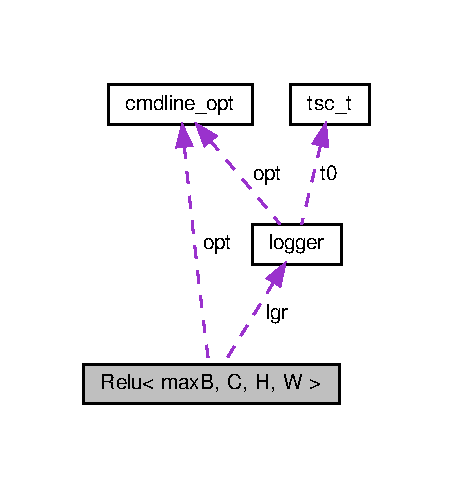
\includegraphics[width=218pt]{structRelu__coll__graph}
\end{center}
\end{figure}
\subsection*{Public Member Functions}
\begin{DoxyCompactItemize}
\item 
void \hyperlink{structRelu_af79e0373854c503faeda1928c0950b9b}{init} (\hyperlink{structcmdline__opt}{cmdline\+\_\+opt} \hyperlink{structRelu_a63f877be5c3cf3b8c89b57dbf2da0e68}{opt}, \hyperlink{structlogger}{logger} $\ast$\hyperlink{structRelu_af0064c033b32a241427e76c25b2eee41}{lgr})
\begin{DoxyCompactList}\small\item\em initialize \end{DoxyCompactList}\item 
\hyperlink{structRelu}{Relu}$<$ maxB, C, H, W $>$ $\ast$ \hyperlink{structRelu_ac5d197a3266cc0d939bc0d54ab23df9f}{copy} ()
\begin{DoxyCompactList}\small\item\em make a copy of this \end{DoxyCompactList}\item 
void \hyperlink{structRelu_a4e32ca92b471641ee2d5c1a252bab167}{set\+\_\+dev} (\hyperlink{structRelu}{Relu}$<$ maxB, C, H, W $>$ $\ast$\hyperlink{structRelu_a1e1271caca013c95ece064b47196d100}{dev})
\begin{DoxyCompactList}\small\item\em set the device pointer for this and all subobjects \end{DoxyCompactList}\item 
void \hyperlink{structRelu_a0109665896b86defceb3b7b5f4869075}{make\+\_\+dev} ()
\begin{DoxyCompactList}\small\item\em if the algorithm is a gpu algorithm, allocate a device shadow of this object and set dev field of this and all subobjects. otherwise it sets all dev fields to null. \end{DoxyCompactList}\item 
void \hyperlink{structRelu_a449f220c5cd23217aa463f68a8a4933a}{del\+\_\+dev} ()
\begin{DoxyCompactList}\small\item\em if the algorithm is a gpu algorithm, dev field must not be null and deallocate it. \end{DoxyCompactList}\item 
\mbox{\Hypertarget{structRelu_aa039e9ae5722c8930b80fa9e44bf1b9d}\label{structRelu_aa039e9ae5722c8930b80fa9e44bf1b9d}} 
void \hyperlink{structRelu_aa039e9ae5722c8930b80fa9e44bf1b9d}{to\+\_\+dev} ()
\begin{DoxyCompactList}\small\item\em if the algorithm is a gpu algorithm, dev field must not be null and send the host data to the device memory \end{DoxyCompactList}\item 
\mbox{\Hypertarget{structRelu_a6c751671bf87512e622d6d42301b2663}\label{structRelu_a6c751671bf87512e622d6d42301b2663}} 
void \hyperlink{structRelu_a6c751671bf87512e622d6d42301b2663}{to\+\_\+host} ()
\begin{DoxyCompactList}\small\item\em if the algorithm is a gpu algorithm, dev field must not be null and send the device data to the host memory \end{DoxyCompactList}\item 
\+\_\+\+\_\+device\+\_\+\+\_\+ \+\_\+\+\_\+host\+\_\+\+\_\+ void \hyperlink{structRelu_a41981da3c54691ae68933d5802a6518b}{forward\+\_\+base} (\hyperlink{structarray4}{array4}$<$ maxB, C, H, W $>$ \&x)
\begin{DoxyCompactList}\small\item\em the baseline (serial) implementation of forward called both by cpu implementation (forward\+\_\+cpu) and gpu implementation (forward\+\_\+dev). the call sequence forward -\/$>$ forward\+\_\+cpu -\/$>$ forward\+\_\+base on cpu and and is forward -\/$>$ forward\+\_\+gpu -\/$>$ forward\+\_\+global -\/$>$ forward\+\_\+dev -\/$>$ forward\+\_\+base \end{DoxyCompactList}\item 
\+\_\+\+\_\+device\+\_\+\+\_\+ void \hyperlink{structRelu_aba6323a49a9e24b29bbb18b27707bae8}{forward\+\_\+dev} (\hyperlink{structarray4}{array4}$<$ maxB, C, H, W $>$ \&x)
\begin{DoxyCompactList}\small\item\em the device function of forward called from the global (non-\/member) function \end{DoxyCompactList}\item 
void \hyperlink{structRelu_a555ae5bc02822f294cac68cf3fe94e84}{forward\+\_\+gpu} (\hyperlink{structarray4}{array4}$<$ maxB, C, H, W $>$ \&x)
\begin{DoxyCompactList}\small\item\em a gpu version of baseline code called from the entry function (forward) \end{DoxyCompactList}\item 
void \hyperlink{structRelu_a767ca23ba58264771274f2e5e51ae4ce}{forward\+\_\+cpu} (\hyperlink{structarray4}{array4}$<$ maxB, C, H, W $>$ \&x)
\begin{DoxyCompactList}\small\item\em a cpu version of baseline code called from the entry function (forward) \end{DoxyCompactList}\item 
\hyperlink{structarray4}{array4}$<$ maxB, C, H, W $>$ \& \hyperlink{structRelu_a71f8322b10508a210025151ad788226f}{forward} (\hyperlink{structarray4}{array4}$<$ maxB, C, H, W $>$ \&x)
\begin{DoxyCompactList}\small\item\em calc the loss function of a mini-\/batch (x) \end{DoxyCompactList}\item 
\+\_\+\+\_\+device\+\_\+\+\_\+ \+\_\+\+\_\+host\+\_\+\+\_\+ void \hyperlink{structRelu_ad2da72c21984db8c9cec57c6d60bf741}{backward\+\_\+base} (\hyperlink{structarray4}{array4}$<$ maxB, C, H, W $>$ \&gy)
\begin{DoxyCompactList}\small\item\em the baseline (serial) implementation of backward called both by cpu implementation (backward\+\_\+cpu) and gpu implementation (backward\+\_\+dev). the call sequence backward -\/$>$ backward\+\_\+cpu -\/$>$ backward\+\_\+base on cpu and and is backward -\/$>$ backward\+\_\+gpu -\/$>$ backward\+\_\+global -\/$>$ backward\+\_\+dev -\/$>$ backward\+\_\+base \end{DoxyCompactList}\item 
\+\_\+\+\_\+device\+\_\+\+\_\+ void \hyperlink{structRelu_a0b13992d8093aa08ed9036cac3a5437b}{backward\+\_\+dev} (\hyperlink{structarray4}{array4}$<$ maxB, C, H, W $>$ \&gy)
\begin{DoxyCompactList}\small\item\em the device function of backward called from the global (non-\/member) function \end{DoxyCompactList}\item 
void \hyperlink{structRelu_a15ee109a34e8ad3c94c0b42c05647342}{backward\+\_\+gpu} (\hyperlink{structarray4}{array4}$<$ maxB, C, H, W $>$ \&gy)
\begin{DoxyCompactList}\small\item\em a gpu version of baseline code called from the entry function (backward) \end{DoxyCompactList}\item 
void \hyperlink{structRelu_aa2112a7ad1cb1faea9babc90835a84c5}{backward\+\_\+cpu} (\hyperlink{structarray4}{array4}$<$ maxB, C, H, W $>$ \&gy)
\begin{DoxyCompactList}\small\item\em a cpu version of baseline code called from the entry function (backward) \end{DoxyCompactList}\item 
\hyperlink{structarray4}{array4}$<$ maxB, C, H, W $>$ \& \hyperlink{structRelu_af9d3182c5103542c1c9796edc449847c}{backward} (\hyperlink{structarray4}{array4}$<$ maxB, C, H, W $>$ \&gy)
\begin{DoxyCompactList}\small\item\em calc the gradient of loss wrt the input (x) \end{DoxyCompactList}\end{DoxyCompactItemize}
\subsection*{Public Attributes}
\begin{DoxyCompactItemize}
\item 
\hyperlink{structRelu}{Relu}$<$ maxB, C, H, W $>$ $\ast$ \hyperlink{structRelu_a1e1271caca013c95ece064b47196d100}{dev}
\item 
\hyperlink{structcmdline__opt}{cmdline\+\_\+opt} \hyperlink{structRelu_a63f877be5c3cf3b8c89b57dbf2da0e68}{opt}
\item 
\hyperlink{structlogger}{logger} $\ast$ \hyperlink{structRelu_af0064c033b32a241427e76c25b2eee41}{lgr}
\item 
\hyperlink{structarray4}{array4}$<$ maxB, C, H, W $>$ $\ast$ \hyperlink{structRelu_a51ae894a609b5de1e41e8fd30ff5575c}{x\+\_\+ptr}
\item 
\hyperlink{structarray4}{array4}$<$ maxB, C, H, W $>$ \hyperlink{structRelu_a30148be5eabe65c95a37c7cd0525c08a}{y}
\item 
\hyperlink{structarray4}{array4}$<$ maxB, C, H, W $>$ \hyperlink{structRelu_a0e864208d70a5d7976a71c87a54c7edf}{gx}
\end{DoxyCompactItemize}


\subsection{Detailed Description}
\subsubsection*{template$<$idx\+\_\+t maxB, idx\+\_\+t C, idx\+\_\+t H, idx\+\_\+t W$>$\newline
struct Relu$<$ max\+B, C, H, W $>$}

dropout layer 


\begin{DoxyParams}{Parameters}
{\em (max\+B)} & the maximum number of images (batch size) \\
\hline
{\em (\+C)} & the number of channels per input image (the original input has typically three channels for R\+GB. in hidden layers, it starts from 64 and goes up to 512 in the last hidden layer) \\
\hline
{\em (\+H)} & height of an image (32 for an input image, down to 1 in the last hidden layer) \\
\hline
{\em (\+W)} & width of an image (32 for an input image, down to 1 in the last hidden layer)\\
\hline
\end{DoxyParams}
this layer normalizes a batch of images 

\subsection{Member Function Documentation}
\mbox{\Hypertarget{structRelu_af9d3182c5103542c1c9796edc449847c}\label{structRelu_af9d3182c5103542c1c9796edc449847c}} 
\index{Relu@{Relu}!backward@{backward}}
\index{backward@{backward}!Relu@{Relu}}
\subsubsection{\texorpdfstring{backward()}{backward()}}
{\footnotesize\ttfamily template$<$idx\+\_\+t maxB, idx\+\_\+t C, idx\+\_\+t H, idx\+\_\+t W$>$ \\
\hyperlink{structarray4}{array4}$<$maxB,C,H,W$>$\& \hyperlink{structRelu}{Relu}$<$ maxB, C, H, W $>$\+::backward (\begin{DoxyParamCaption}\item[{\hyperlink{structarray4}{array4}$<$ maxB, C, H, W $>$ \&}]{gy }\end{DoxyParamCaption})\hspace{0.3cm}{\ttfamily [inline]}}



calc the gradient of loss wrt the input (x) 


\begin{DoxyParams}{Parameters}
{\em (gy)} & gradient of loss with respect to the output\\
\hline
\end{DoxyParams}
calc the gradient of loss wrt the input. along the way, it also calculates the gradient of loss wrt weights for all sublayers that have weights. since this is the entire network, gy is actually a vector whose components are all 1. (loss = sum of losses of each data). \begin{DoxySeeAlso}{See also}
\hyperlink{structRelu_a71f8322b10508a210025151ad788226f}{forward} 

update 
\end{DoxySeeAlso}
\mbox{\Hypertarget{structRelu_ad2da72c21984db8c9cec57c6d60bf741}\label{structRelu_ad2da72c21984db8c9cec57c6d60bf741}} 
\index{Relu@{Relu}!backward\+\_\+base@{backward\+\_\+base}}
\index{backward\+\_\+base@{backward\+\_\+base}!Relu@{Relu}}
\subsubsection{\texorpdfstring{backward\+\_\+base()}{backward\_base()}}
{\footnotesize\ttfamily template$<$idx\+\_\+t maxB, idx\+\_\+t C, idx\+\_\+t H, idx\+\_\+t W$>$ \\
\+\_\+\+\_\+device\+\_\+\+\_\+ \+\_\+\+\_\+host\+\_\+\+\_\+ void \hyperlink{structRelu}{Relu}$<$ maxB, C, H, W $>$\+::backward\+\_\+base (\begin{DoxyParamCaption}\item[{\hyperlink{structarray4}{array4}$<$ maxB, C, H, W $>$ \&}]{gy }\end{DoxyParamCaption})\hspace{0.3cm}{\ttfamily [inline]}}



the baseline (serial) implementation of backward called both by cpu implementation (backward\+\_\+cpu) and gpu implementation (backward\+\_\+dev). the call sequence backward -\/$>$ backward\+\_\+cpu -\/$>$ backward\+\_\+base on cpu and and is backward -\/$>$ backward\+\_\+gpu -\/$>$ backward\+\_\+global -\/$>$ backward\+\_\+dev -\/$>$ backward\+\_\+base 


\begin{DoxyParams}{Parameters}
{\em (gy)} & gradient of loss with respect to the output \\
\hline
\end{DoxyParams}
\begin{DoxySeeAlso}{See also}
\hyperlink{structRelu_af9d3182c5103542c1c9796edc449847c}{backward} 

\hyperlink{structRelu_a15ee109a34e8ad3c94c0b42c05647342}{backward\+\_\+gpu} 

\hyperlink{softmaxcrossentropy_8h_a47d56a9a23e08247b227f4aac17413e0}{backward\+\_\+global} 

\hyperlink{structRelu_a0b13992d8093aa08ed9036cac3a5437b}{backward\+\_\+dev} 
\end{DoxySeeAlso}
\mbox{\Hypertarget{structRelu_aa2112a7ad1cb1faea9babc90835a84c5}\label{structRelu_aa2112a7ad1cb1faea9babc90835a84c5}} 
\index{Relu@{Relu}!backward\+\_\+cpu@{backward\+\_\+cpu}}
\index{backward\+\_\+cpu@{backward\+\_\+cpu}!Relu@{Relu}}
\subsubsection{\texorpdfstring{backward\+\_\+cpu()}{backward\_cpu()}}
{\footnotesize\ttfamily template$<$idx\+\_\+t maxB, idx\+\_\+t C, idx\+\_\+t H, idx\+\_\+t W$>$ \\
void \hyperlink{structRelu}{Relu}$<$ maxB, C, H, W $>$\+::backward\+\_\+cpu (\begin{DoxyParamCaption}\item[{\hyperlink{structarray4}{array4}$<$ maxB, C, H, W $>$ \&}]{gy }\end{DoxyParamCaption})\hspace{0.3cm}{\ttfamily [inline]}}



a cpu version of baseline code called from the entry function (backward) 


\begin{DoxyParams}{Parameters}
{\em (gy)} & gradient of loss with respect to the output \\
\hline
\end{DoxyParams}
\begin{DoxySeeAlso}{See also}
\hyperlink{structRelu_af9d3182c5103542c1c9796edc449847c}{backward} 

\hyperlink{structRelu_ad2da72c21984db8c9cec57c6d60bf741}{backward\+\_\+base} 
\end{DoxySeeAlso}
\mbox{\Hypertarget{structRelu_a0b13992d8093aa08ed9036cac3a5437b}\label{structRelu_a0b13992d8093aa08ed9036cac3a5437b}} 
\index{Relu@{Relu}!backward\+\_\+dev@{backward\+\_\+dev}}
\index{backward\+\_\+dev@{backward\+\_\+dev}!Relu@{Relu}}
\subsubsection{\texorpdfstring{backward\+\_\+dev()}{backward\_dev()}}
{\footnotesize\ttfamily template$<$idx\+\_\+t maxB, idx\+\_\+t C, idx\+\_\+t H, idx\+\_\+t W$>$ \\
\+\_\+\+\_\+device\+\_\+\+\_\+ void \hyperlink{structRelu}{Relu}$<$ maxB, C, H, W $>$\+::backward\+\_\+dev (\begin{DoxyParamCaption}\item[{\hyperlink{structarray4}{array4}$<$ maxB, C, H, W $>$ \&}]{gy }\end{DoxyParamCaption})\hspace{0.3cm}{\ttfamily [inline]}}



the device function of backward called from the global (non-\/member) function 


\begin{DoxyParams}{Parameters}
{\em (gy)} & gradient of loss with respect to the output \\
\hline
\end{DoxyParams}
\begin{DoxySeeAlso}{See also}
\hyperlink{structRelu_af9d3182c5103542c1c9796edc449847c}{backward} 

\hyperlink{structRelu_a15ee109a34e8ad3c94c0b42c05647342}{backward\+\_\+gpu} 

\hyperlink{softmaxcrossentropy_8h_a47d56a9a23e08247b227f4aac17413e0}{backward\+\_\+global} 

\hyperlink{structRelu_ad2da72c21984db8c9cec57c6d60bf741}{backward\+\_\+base} 
\end{DoxySeeAlso}
\mbox{\Hypertarget{structRelu_a15ee109a34e8ad3c94c0b42c05647342}\label{structRelu_a15ee109a34e8ad3c94c0b42c05647342}} 
\index{Relu@{Relu}!backward\+\_\+gpu@{backward\+\_\+gpu}}
\index{backward\+\_\+gpu@{backward\+\_\+gpu}!Relu@{Relu}}
\subsubsection{\texorpdfstring{backward\+\_\+gpu()}{backward\_gpu()}}
{\footnotesize\ttfamily template$<$idx\+\_\+t maxB, idx\+\_\+t C, idx\+\_\+t H, idx\+\_\+t W$>$ \\
void \hyperlink{structRelu}{Relu}$<$ maxB, C, H, W $>$\+::backward\+\_\+gpu (\begin{DoxyParamCaption}\item[{\hyperlink{structarray4}{array4}$<$ maxB, C, H, W $>$ \&}]{gy }\end{DoxyParamCaption})\hspace{0.3cm}{\ttfamily [inline]}}



a gpu version of baseline code called from the entry function (backward) 


\begin{DoxyParams}{Parameters}
{\em (gy)} & gradient of loss with respect to the output \\
\hline
\end{DoxyParams}
\begin{DoxySeeAlso}{See also}
\hyperlink{structRelu_af9d3182c5103542c1c9796edc449847c}{backward} 

\hyperlink{softmaxcrossentropy_8h_a47d56a9a23e08247b227f4aac17413e0}{backward\+\_\+global} 

\hyperlink{structRelu_a0b13992d8093aa08ed9036cac3a5437b}{backward\+\_\+dev} 

\hyperlink{structRelu_ad2da72c21984db8c9cec57c6d60bf741}{backward\+\_\+base} 
\end{DoxySeeAlso}
\mbox{\Hypertarget{structRelu_ac5d197a3266cc0d939bc0d54ab23df9f}\label{structRelu_ac5d197a3266cc0d939bc0d54ab23df9f}} 
\index{Relu@{Relu}!copy@{copy}}
\index{copy@{copy}!Relu@{Relu}}
\subsubsection{\texorpdfstring{copy()}{copy()}}
{\footnotesize\ttfamily template$<$idx\+\_\+t maxB, idx\+\_\+t C, idx\+\_\+t H, idx\+\_\+t W$>$ \\
\hyperlink{structRelu}{Relu}$<$maxB,C,H,W$>$$\ast$ \hyperlink{structRelu}{Relu}$<$ maxB, C, H, W $>$\+::copy (\begin{DoxyParamCaption}{ }\end{DoxyParamCaption})\hspace{0.3cm}{\ttfamily [inline]}}



make a copy of this 

if this object has a device pointer, the copy will have a device pointer too, but its contents are N\+OT copied \mbox{\Hypertarget{structRelu_a449f220c5cd23217aa463f68a8a4933a}\label{structRelu_a449f220c5cd23217aa463f68a8a4933a}} 
\index{Relu@{Relu}!del\+\_\+dev@{del\+\_\+dev}}
\index{del\+\_\+dev@{del\+\_\+dev}!Relu@{Relu}}
\subsubsection{\texorpdfstring{del\+\_\+dev()}{del\_dev()}}
{\footnotesize\ttfamily template$<$idx\+\_\+t maxB, idx\+\_\+t C, idx\+\_\+t H, idx\+\_\+t W$>$ \\
void \hyperlink{structRelu}{Relu}$<$ maxB, C, H, W $>$\+::del\+\_\+dev (\begin{DoxyParamCaption}{ }\end{DoxyParamCaption})\hspace{0.3cm}{\ttfamily [inline]}}



if the algorithm is a gpu algorithm, dev field must not be null and deallocate it. 

\begin{DoxySeeAlso}{See also}
\hyperlink{structRelu_a0109665896b86defceb3b7b5f4869075}{make\+\_\+dev} 

\hyperlink{structRelu_a4e32ca92b471641ee2d5c1a252bab167}{set\+\_\+dev} 
\end{DoxySeeAlso}
\mbox{\Hypertarget{structRelu_a71f8322b10508a210025151ad788226f}\label{structRelu_a71f8322b10508a210025151ad788226f}} 
\index{Relu@{Relu}!forward@{forward}}
\index{forward@{forward}!Relu@{Relu}}
\subsubsection{\texorpdfstring{forward()}{forward()}}
{\footnotesize\ttfamily template$<$idx\+\_\+t maxB, idx\+\_\+t C, idx\+\_\+t H, idx\+\_\+t W$>$ \\
\hyperlink{structarray4}{array4}$<$maxB,C,H,W$>$\& \hyperlink{structRelu}{Relu}$<$ maxB, C, H, W $>$\+::forward (\begin{DoxyParamCaption}\item[{\hyperlink{structarray4}{array4}$<$ maxB, C, H, W $>$ \&}]{x }\end{DoxyParamCaption})\hspace{0.3cm}{\ttfamily [inline]}}



calc the loss function of a mini-\/batch (x) 


\begin{DoxyParams}{Parameters}
{\em (x)} & input images \\
\hline
\end{DoxyParams}
\begin{DoxySeeAlso}{See also}
\hyperlink{structRelu_af9d3182c5103542c1c9796edc449847c}{backward} 

update 
\end{DoxySeeAlso}
\mbox{\Hypertarget{structRelu_a41981da3c54691ae68933d5802a6518b}\label{structRelu_a41981da3c54691ae68933d5802a6518b}} 
\index{Relu@{Relu}!forward\+\_\+base@{forward\+\_\+base}}
\index{forward\+\_\+base@{forward\+\_\+base}!Relu@{Relu}}
\subsubsection{\texorpdfstring{forward\+\_\+base()}{forward\_base()}}
{\footnotesize\ttfamily template$<$idx\+\_\+t maxB, idx\+\_\+t C, idx\+\_\+t H, idx\+\_\+t W$>$ \\
\+\_\+\+\_\+device\+\_\+\+\_\+ \+\_\+\+\_\+host\+\_\+\+\_\+ void \hyperlink{structRelu}{Relu}$<$ maxB, C, H, W $>$\+::forward\+\_\+base (\begin{DoxyParamCaption}\item[{\hyperlink{structarray4}{array4}$<$ maxB, C, H, W $>$ \&}]{x }\end{DoxyParamCaption})\hspace{0.3cm}{\ttfamily [inline]}}



the baseline (serial) implementation of forward called both by cpu implementation (forward\+\_\+cpu) and gpu implementation (forward\+\_\+dev). the call sequence forward -\/$>$ forward\+\_\+cpu -\/$>$ forward\+\_\+base on cpu and and is forward -\/$>$ forward\+\_\+gpu -\/$>$ forward\+\_\+global -\/$>$ forward\+\_\+dev -\/$>$ forward\+\_\+base 


\begin{DoxyParams}{Parameters}
{\em (x)} & input images \\
\hline
\end{DoxyParams}
\begin{DoxySeeAlso}{See also}
\hyperlink{structRelu_a71f8322b10508a210025151ad788226f}{forward} 

\hyperlink{structRelu_a555ae5bc02822f294cac68cf3fe94e84}{forward\+\_\+gpu} 

\hyperlink{softmaxcrossentropy_8h_a578aeeb166bd06e800d9b396eab48b35}{forward\+\_\+global} 

\hyperlink{structRelu_aba6323a49a9e24b29bbb18b27707bae8}{forward\+\_\+dev} 
\end{DoxySeeAlso}
\mbox{\Hypertarget{structRelu_a767ca23ba58264771274f2e5e51ae4ce}\label{structRelu_a767ca23ba58264771274f2e5e51ae4ce}} 
\index{Relu@{Relu}!forward\+\_\+cpu@{forward\+\_\+cpu}}
\index{forward\+\_\+cpu@{forward\+\_\+cpu}!Relu@{Relu}}
\subsubsection{\texorpdfstring{forward\+\_\+cpu()}{forward\_cpu()}}
{\footnotesize\ttfamily template$<$idx\+\_\+t maxB, idx\+\_\+t C, idx\+\_\+t H, idx\+\_\+t W$>$ \\
void \hyperlink{structRelu}{Relu}$<$ maxB, C, H, W $>$\+::forward\+\_\+cpu (\begin{DoxyParamCaption}\item[{\hyperlink{structarray4}{array4}$<$ maxB, C, H, W $>$ \&}]{x }\end{DoxyParamCaption})\hspace{0.3cm}{\ttfamily [inline]}}



a cpu version of baseline code called from the entry function (forward) 


\begin{DoxyParams}{Parameters}
{\em (x)} & input images \\
\hline
\end{DoxyParams}
\begin{DoxySeeAlso}{See also}
\hyperlink{structRelu_a71f8322b10508a210025151ad788226f}{forward} 

\hyperlink{structRelu_a41981da3c54691ae68933d5802a6518b}{forward\+\_\+base} 
\end{DoxySeeAlso}
\mbox{\Hypertarget{structRelu_aba6323a49a9e24b29bbb18b27707bae8}\label{structRelu_aba6323a49a9e24b29bbb18b27707bae8}} 
\index{Relu@{Relu}!forward\+\_\+dev@{forward\+\_\+dev}}
\index{forward\+\_\+dev@{forward\+\_\+dev}!Relu@{Relu}}
\subsubsection{\texorpdfstring{forward\+\_\+dev()}{forward\_dev()}}
{\footnotesize\ttfamily template$<$idx\+\_\+t maxB, idx\+\_\+t C, idx\+\_\+t H, idx\+\_\+t W$>$ \\
\+\_\+\+\_\+device\+\_\+\+\_\+ void \hyperlink{structRelu}{Relu}$<$ maxB, C, H, W $>$\+::forward\+\_\+dev (\begin{DoxyParamCaption}\item[{\hyperlink{structarray4}{array4}$<$ maxB, C, H, W $>$ \&}]{x }\end{DoxyParamCaption})\hspace{0.3cm}{\ttfamily [inline]}}



the device function of forward called from the global (non-\/member) function 


\begin{DoxyParams}{Parameters}
{\em (x)} & input images \\
\hline
\end{DoxyParams}
\begin{DoxySeeAlso}{See also}
\hyperlink{structRelu_a71f8322b10508a210025151ad788226f}{forward} 

\hyperlink{structRelu_a555ae5bc02822f294cac68cf3fe94e84}{forward\+\_\+gpu} 

\hyperlink{softmaxcrossentropy_8h_a578aeeb166bd06e800d9b396eab48b35}{forward\+\_\+global} 

\hyperlink{structRelu_a41981da3c54691ae68933d5802a6518b}{forward\+\_\+base} 
\end{DoxySeeAlso}
\mbox{\Hypertarget{structRelu_a555ae5bc02822f294cac68cf3fe94e84}\label{structRelu_a555ae5bc02822f294cac68cf3fe94e84}} 
\index{Relu@{Relu}!forward\+\_\+gpu@{forward\+\_\+gpu}}
\index{forward\+\_\+gpu@{forward\+\_\+gpu}!Relu@{Relu}}
\subsubsection{\texorpdfstring{forward\+\_\+gpu()}{forward\_gpu()}}
{\footnotesize\ttfamily template$<$idx\+\_\+t maxB, idx\+\_\+t C, idx\+\_\+t H, idx\+\_\+t W$>$ \\
void \hyperlink{structRelu}{Relu}$<$ maxB, C, H, W $>$\+::forward\+\_\+gpu (\begin{DoxyParamCaption}\item[{\hyperlink{structarray4}{array4}$<$ maxB, C, H, W $>$ \&}]{x }\end{DoxyParamCaption})\hspace{0.3cm}{\ttfamily [inline]}}



a gpu version of baseline code called from the entry function (forward) 


\begin{DoxyParams}{Parameters}
{\em (x)} & input images \\
\hline
\end{DoxyParams}
\begin{DoxySeeAlso}{See also}
\hyperlink{structRelu_a71f8322b10508a210025151ad788226f}{forward} 

\hyperlink{softmaxcrossentropy_8h_a578aeeb166bd06e800d9b396eab48b35}{forward\+\_\+global} 

\hyperlink{structRelu_aba6323a49a9e24b29bbb18b27707bae8}{forward\+\_\+dev} 

\hyperlink{structRelu_a41981da3c54691ae68933d5802a6518b}{forward\+\_\+base} 
\end{DoxySeeAlso}
\mbox{\Hypertarget{structRelu_af79e0373854c503faeda1928c0950b9b}\label{structRelu_af79e0373854c503faeda1928c0950b9b}} 
\index{Relu@{Relu}!init@{init}}
\index{init@{init}!Relu@{Relu}}
\subsubsection{\texorpdfstring{init()}{init()}}
{\footnotesize\ttfamily template$<$idx\+\_\+t maxB, idx\+\_\+t C, idx\+\_\+t H, idx\+\_\+t W$>$ \\
void \hyperlink{structRelu}{Relu}$<$ maxB, C, H, W $>$\+::init (\begin{DoxyParamCaption}\item[{\hyperlink{structcmdline__opt}{cmdline\+\_\+opt}}]{opt,  }\item[{\hyperlink{structlogger}{logger} $\ast$}]{lgr }\end{DoxyParamCaption})\hspace{0.3cm}{\ttfamily [inline]}}



initialize 


\begin{DoxyParams}{Parameters}
{\em (opt)} & command line options \\
\hline
{\em (lgr)} & logger \\
\hline
\end{DoxyParams}
\mbox{\Hypertarget{structRelu_a0109665896b86defceb3b7b5f4869075}\label{structRelu_a0109665896b86defceb3b7b5f4869075}} 
\index{Relu@{Relu}!make\+\_\+dev@{make\+\_\+dev}}
\index{make\+\_\+dev@{make\+\_\+dev}!Relu@{Relu}}
\subsubsection{\texorpdfstring{make\+\_\+dev()}{make\_dev()}}
{\footnotesize\ttfamily template$<$idx\+\_\+t maxB, idx\+\_\+t C, idx\+\_\+t H, idx\+\_\+t W$>$ \\
void \hyperlink{structRelu}{Relu}$<$ maxB, C, H, W $>$\+::make\+\_\+dev (\begin{DoxyParamCaption}{ }\end{DoxyParamCaption})\hspace{0.3cm}{\ttfamily [inline]}}



if the algorithm is a gpu algorithm, allocate a device shadow of this object and set dev field of this and all subobjects. otherwise it sets all dev fields to null. 

\begin{DoxySeeAlso}{See also}
\hyperlink{structRelu_a4e32ca92b471641ee2d5c1a252bab167}{set\+\_\+dev} 

\hyperlink{structRelu_a449f220c5cd23217aa463f68a8a4933a}{del\+\_\+dev} 
\end{DoxySeeAlso}
\mbox{\Hypertarget{structRelu_a4e32ca92b471641ee2d5c1a252bab167}\label{structRelu_a4e32ca92b471641ee2d5c1a252bab167}} 
\index{Relu@{Relu}!set\+\_\+dev@{set\+\_\+dev}}
\index{set\+\_\+dev@{set\+\_\+dev}!Relu@{Relu}}
\subsubsection{\texorpdfstring{set\+\_\+dev()}{set\_dev()}}
{\footnotesize\ttfamily template$<$idx\+\_\+t maxB, idx\+\_\+t C, idx\+\_\+t H, idx\+\_\+t W$>$ \\
void \hyperlink{structRelu}{Relu}$<$ maxB, C, H, W $>$\+::set\+\_\+dev (\begin{DoxyParamCaption}\item[{\hyperlink{structRelu}{Relu}$<$ maxB, C, H, W $>$ $\ast$}]{dev }\end{DoxyParamCaption})\hspace{0.3cm}{\ttfamily [inline]}}



set the device pointer for this and all subobjects 


\begin{DoxyParams}{Parameters}
{\em (dev)} & a device memory or null \\
\hline
\end{DoxyParams}
\begin{DoxySeeAlso}{See also}
\hyperlink{structRelu_a0109665896b86defceb3b7b5f4869075}{make\+\_\+dev} 

\hyperlink{structRelu_a449f220c5cd23217aa463f68a8a4933a}{del\+\_\+dev}
\end{DoxySeeAlso}
if dev is not null, dev fields of all subojects point to the corresponding subjects in the device memory. if dev is not null, all dev fields become null. 

\subsection{Member Data Documentation}
\mbox{\Hypertarget{structRelu_a1e1271caca013c95ece064b47196d100}\label{structRelu_a1e1271caca013c95ece064b47196d100}} 
\index{Relu@{Relu}!dev@{dev}}
\index{dev@{dev}!Relu@{Relu}}
\subsubsection{\texorpdfstring{dev}{dev}}
{\footnotesize\ttfamily template$<$idx\+\_\+t maxB, idx\+\_\+t C, idx\+\_\+t H, idx\+\_\+t W$>$ \\
\hyperlink{structRelu}{Relu}$<$maxB,C,H,W$>$$\ast$ \hyperlink{structRelu}{Relu}$<$ maxB, C, H, W $>$\+::dev}

device shadow \mbox{\Hypertarget{structRelu_a0e864208d70a5d7976a71c87a54c7edf}\label{structRelu_a0e864208d70a5d7976a71c87a54c7edf}} 
\index{Relu@{Relu}!gx@{gx}}
\index{gx@{gx}!Relu@{Relu}}
\subsubsection{\texorpdfstring{gx}{gx}}
{\footnotesize\ttfamily template$<$idx\+\_\+t maxB, idx\+\_\+t C, idx\+\_\+t H, idx\+\_\+t W$>$ \\
\hyperlink{structarray4}{array4}$<$maxB,C,H,W$>$ \hyperlink{structRelu}{Relu}$<$ maxB, C, H, W $>$\+::gx}

gradient of loss wrt input x \mbox{\Hypertarget{structRelu_af0064c033b32a241427e76c25b2eee41}\label{structRelu_af0064c033b32a241427e76c25b2eee41}} 
\index{Relu@{Relu}!lgr@{lgr}}
\index{lgr@{lgr}!Relu@{Relu}}
\subsubsection{\texorpdfstring{lgr}{lgr}}
{\footnotesize\ttfamily template$<$idx\+\_\+t maxB, idx\+\_\+t C, idx\+\_\+t H, idx\+\_\+t W$>$ \\
\hyperlink{structlogger}{logger}$\ast$ \hyperlink{structRelu}{Relu}$<$ maxB, C, H, W $>$\+::lgr}

logger \mbox{\Hypertarget{structRelu_a63f877be5c3cf3b8c89b57dbf2da0e68}\label{structRelu_a63f877be5c3cf3b8c89b57dbf2da0e68}} 
\index{Relu@{Relu}!opt@{opt}}
\index{opt@{opt}!Relu@{Relu}}
\subsubsection{\texorpdfstring{opt}{opt}}
{\footnotesize\ttfamily template$<$idx\+\_\+t maxB, idx\+\_\+t C, idx\+\_\+t H, idx\+\_\+t W$>$ \\
\hyperlink{structcmdline__opt}{cmdline\+\_\+opt} \hyperlink{structRelu}{Relu}$<$ maxB, C, H, W $>$\+::opt}

command line option \mbox{\Hypertarget{structRelu_a51ae894a609b5de1e41e8fd30ff5575c}\label{structRelu_a51ae894a609b5de1e41e8fd30ff5575c}} 
\index{Relu@{Relu}!x\+\_\+ptr@{x\+\_\+ptr}}
\index{x\+\_\+ptr@{x\+\_\+ptr}!Relu@{Relu}}
\subsubsection{\texorpdfstring{x\+\_\+ptr}{x\_ptr}}
{\footnotesize\ttfamily template$<$idx\+\_\+t maxB, idx\+\_\+t C, idx\+\_\+t H, idx\+\_\+t W$>$ \\
\hyperlink{structarray4}{array4}$<$maxB,C,H,W$>$$\ast$ \hyperlink{structRelu}{Relu}$<$ maxB, C, H, W $>$\+::x\+\_\+ptr}

pointer to input passed to forward \mbox{\Hypertarget{structRelu_a30148be5eabe65c95a37c7cd0525c08a}\label{structRelu_a30148be5eabe65c95a37c7cd0525c08a}} 
\index{Relu@{Relu}!y@{y}}
\index{y@{y}!Relu@{Relu}}
\subsubsection{\texorpdfstring{y}{y}}
{\footnotesize\ttfamily template$<$idx\+\_\+t maxB, idx\+\_\+t C, idx\+\_\+t H, idx\+\_\+t W$>$ \\
\hyperlink{structarray4}{array4}$<$maxB,C,H,W$>$ \hyperlink{structRelu}{Relu}$<$ maxB, C, H, W $>$\+::y}

output of the forward 

The documentation for this struct was generated from the following file\+:\begin{DoxyCompactItemize}
\item 
/home/tau/public\+\_\+html/lecture/parallel\+\_\+distributed/2018/handson/tau/parallel-\/distributed-\/handson/20vgg/include/\hyperlink{relu_8h}{relu.\+h}\end{DoxyCompactItemize}

\hypertarget{structrnd__gen__t}{}\section{rnd\+\_\+gen\+\_\+t Struct Reference}
\label{structrnd__gen__t}\index{rnd\+\_\+gen\+\_\+t@{rnd\+\_\+gen\+\_\+t}}


pseudo random number generator crafted from man erand48 + libc source  




{\ttfamily \#include $<$vgg\+\_\+util.\+h$>$}

\subsection*{Public Member Functions}
\begin{DoxyCompactItemize}
\item 
\mbox{\Hypertarget{structrnd__gen__t_a681dc7d8fb26a098dd79b00a731565e1}\label{structrnd__gen__t_a681dc7d8fb26a098dd79b00a731565e1}} 
\+\_\+\+\_\+device\+\_\+\+\_\+ \+\_\+\+\_\+host\+\_\+\+\_\+ void \hyperlink{structrnd__gen__t_a681dc7d8fb26a098dd79b00a731565e1}{next} ()
\begin{DoxyCompactList}\small\item\em set next state \end{DoxyCompactList}\item 
\mbox{\Hypertarget{structrnd__gen__t_abcddd9ef63e9228770b4e6a77f1aaaa8}\label{structrnd__gen__t_abcddd9ef63e9228770b4e6a77f1aaaa8}} 
\+\_\+\+\_\+device\+\_\+\+\_\+ \+\_\+\+\_\+host\+\_\+\+\_\+ double \hyperlink{structrnd__gen__t_abcddd9ef63e9228770b4e6a77f1aaaa8}{rand01} ()
\begin{DoxyCompactList}\small\item\em return a random number between 0 and 1 \end{DoxyCompactList}\item 
\mbox{\Hypertarget{structrnd__gen__t_abb4b48e7a93b53df5af70476c07fe76f}\label{structrnd__gen__t_abb4b48e7a93b53df5af70476c07fe76f}} 
\+\_\+\+\_\+device\+\_\+\+\_\+ \+\_\+\+\_\+host\+\_\+\+\_\+ long \hyperlink{structrnd__gen__t_abb4b48e7a93b53df5af70476c07fe76f}{randi32} ()
\begin{DoxyCompactList}\small\item\em return a long between 0 to 2$^\wedge$31 -\/ 1 \end{DoxyCompactList}\item 
\mbox{\Hypertarget{structrnd__gen__t_a0ccf64e18ecb0f64349863ec6883d9c2}\label{structrnd__gen__t_a0ccf64e18ecb0f64349863ec6883d9c2}} 
\+\_\+\+\_\+device\+\_\+\+\_\+ \+\_\+\+\_\+host\+\_\+\+\_\+ double \hyperlink{structrnd__gen__t_a0ccf64e18ecb0f64349863ec6883d9c2}{rand} (double a, double b)
\begin{DoxyCompactList}\small\item\em return a real between a and b \end{DoxyCompactList}\item 
\mbox{\Hypertarget{structrnd__gen__t_ae8f219398f4cf6b4db8b00ea390cf97b}\label{structrnd__gen__t_ae8f219398f4cf6b4db8b00ea390cf97b}} 
\+\_\+\+\_\+device\+\_\+\+\_\+ \+\_\+\+\_\+host\+\_\+\+\_\+ long \hyperlink{structrnd__gen__t_ae8f219398f4cf6b4db8b00ea390cf97b}{randi} (long a, long b)
\begin{DoxyCompactList}\small\item\em return a long between a and b \end{DoxyCompactList}\item 
\+\_\+\+\_\+device\+\_\+\+\_\+ \+\_\+\+\_\+host\+\_\+\+\_\+ \hyperlink{vgg__util_8h_a1082d08aaa761215ec83e7149f27ad16}{real} \hyperlink{structrnd__gen__t_a6015e76eb30c192e3b64a9bc2b546535}{rand\+\_\+normal} (\hyperlink{vgg__util_8h_a1082d08aaa761215ec83e7149f27ad16}{real} mu, \hyperlink{vgg__util_8h_a1082d08aaa761215ec83e7149f27ad16}{real} sigma)
\begin{DoxyCompactList}\small\item\em generate a random number from a normal distribution of mean=mu and standard deviation=sigma. \end{DoxyCompactList}\item 
\mbox{\Hypertarget{structrnd__gen__t_a45c7eb16a8f87359f70e007a00cf92e4}\label{structrnd__gen__t_a45c7eb16a8f87359f70e007a00cf92e4}} 
\+\_\+\+\_\+device\+\_\+\+\_\+ \+\_\+\+\_\+host\+\_\+\+\_\+ long \hyperlink{structrnd__gen__t_a45c7eb16a8f87359f70e007a00cf92e4}{get\+\_\+state} ()
\begin{DoxyCompactList}\small\item\em return the current state of the generator \end{DoxyCompactList}\item 
\mbox{\Hypertarget{structrnd__gen__t_a0e43f9b2d156cb2535bfa1a88cd9eb25}\label{structrnd__gen__t_a0e43f9b2d156cb2535bfa1a88cd9eb25}} 
\+\_\+\+\_\+device\+\_\+\+\_\+ \+\_\+\+\_\+host\+\_\+\+\_\+ void \hyperlink{structrnd__gen__t_a0e43f9b2d156cb2535bfa1a88cd9eb25}{seed} (uint64\+\_\+t y)
\begin{DoxyCompactList}\small\item\em set state of the generator \end{DoxyCompactList}\end{DoxyCompactItemize}
\subsection*{Public Attributes}
\begin{DoxyCompactItemize}
\item 
uint64\+\_\+t \hyperlink{structrnd__gen__t_a80b2d559c8a8046b6e979840ad3379be}{x}
\end{DoxyCompactItemize}


\subsection{Detailed Description}
pseudo random number generator crafted from man erand48 + libc source 

\subsection{Member Function Documentation}
\mbox{\Hypertarget{structrnd__gen__t_a6015e76eb30c192e3b64a9bc2b546535}\label{structrnd__gen__t_a6015e76eb30c192e3b64a9bc2b546535}} 
\index{rnd\+\_\+gen\+\_\+t@{rnd\+\_\+gen\+\_\+t}!rand\+\_\+normal@{rand\+\_\+normal}}
\index{rand\+\_\+normal@{rand\+\_\+normal}!rnd\+\_\+gen\+\_\+t@{rnd\+\_\+gen\+\_\+t}}
\subsubsection{\texorpdfstring{rand\+\_\+normal()}{rand\_normal()}}
{\footnotesize\ttfamily \+\_\+\+\_\+device\+\_\+\+\_\+ \+\_\+\+\_\+host\+\_\+\+\_\+ \hyperlink{vgg__util_8h_a1082d08aaa761215ec83e7149f27ad16}{real} rnd\+\_\+gen\+\_\+t\+::rand\+\_\+normal (\begin{DoxyParamCaption}\item[{\hyperlink{vgg__util_8h_a1082d08aaa761215ec83e7149f27ad16}{real}}]{mu,  }\item[{\hyperlink{vgg__util_8h_a1082d08aaa761215ec83e7149f27ad16}{real}}]{sigma }\end{DoxyParamCaption})\hspace{0.3cm}{\ttfamily [inline]}}



generate a random number from a normal distribution of mean=mu and standard deviation=sigma. 

see \href{https://en.wikipedia.org/wiki/Normal_distribution}{\tt https\+://en.\+wikipedia.\+org/wiki/\+Normal\+\_\+distribution} for how the following method works 

\subsection{Member Data Documentation}
\mbox{\Hypertarget{structrnd__gen__t_a80b2d559c8a8046b6e979840ad3379be}\label{structrnd__gen__t_a80b2d559c8a8046b6e979840ad3379be}} 
\index{rnd\+\_\+gen\+\_\+t@{rnd\+\_\+gen\+\_\+t}!x@{x}}
\index{x@{x}!rnd\+\_\+gen\+\_\+t@{rnd\+\_\+gen\+\_\+t}}
\subsubsection{\texorpdfstring{x}{x}}
{\footnotesize\ttfamily uint64\+\_\+t rnd\+\_\+gen\+\_\+t\+::x}

random number state 

The documentation for this struct was generated from the following file\+:\begin{DoxyCompactItemize}
\item 
/home/tau/public\+\_\+html/lecture/parallel\+\_\+distributed/2018/handson/tau/parallel-\/distributed-\/handson/20vgg/include/\hyperlink{vgg__util_8h}{vgg\+\_\+util.\+h}\end{DoxyCompactItemize}

\hypertarget{structSoftmaxCrossEntropy}{}\section{Softmax\+Cross\+Entropy$<$ maxB, nC $>$ Struct Template Reference}
\label{structSoftmaxCrossEntropy}\index{Softmax\+Cross\+Entropy$<$ max\+B, n\+C $>$@{Softmax\+Cross\+Entropy$<$ max\+B, n\+C $>$}}


dropout layer  




{\ttfamily \#include $<$softmaxcrossentropy.\+h$>$}



Collaboration diagram for Softmax\+Cross\+Entropy$<$ maxB, nC $>$\+:
\nopagebreak
\begin{figure}[H]
\begin{center}
\leavevmode
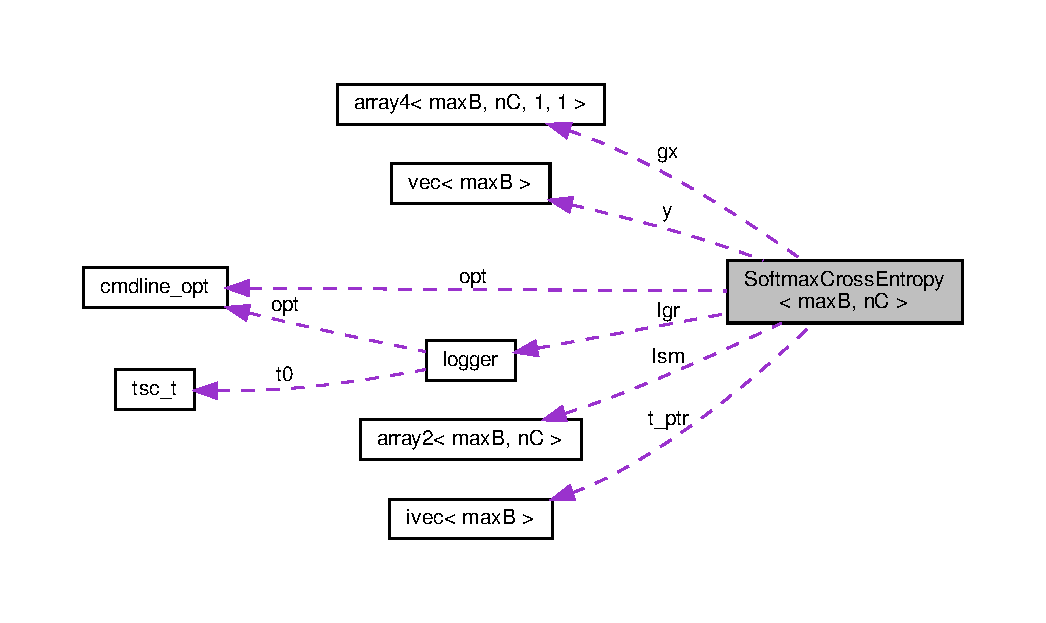
\includegraphics[width=350pt]{structSoftmaxCrossEntropy__coll__graph}
\end{center}
\end{figure}
\subsection*{Public Member Functions}
\begin{DoxyCompactItemize}
\item 
void \hyperlink{structSoftmaxCrossEntropy_ad531aa32fa665c1596f686eae4b8e008}{init} (\hyperlink{structcmdline__opt}{cmdline\+\_\+opt} \hyperlink{structSoftmaxCrossEntropy_a5b1fcafb5b11b7c6c09c228fb442a888}{opt}, \hyperlink{structlogger}{logger} $\ast$\hyperlink{structSoftmaxCrossEntropy_a10a76ce6a1cd3e1d1a57c0f2ba42f5a0}{lgr})
\begin{DoxyCompactList}\small\item\em initialize \end{DoxyCompactList}\item 
\hyperlink{structSoftmaxCrossEntropy}{Softmax\+Cross\+Entropy}$<$ maxB, nC $>$ $\ast$ \hyperlink{structSoftmaxCrossEntropy_aa152e1e400520acefcaa8bfa0999fce7}{copy} ()
\begin{DoxyCompactList}\small\item\em make a copy of this \end{DoxyCompactList}\item 
void \hyperlink{structSoftmaxCrossEntropy_a2fd71f3001bb7a06f4f4c2902c43b657}{set\+\_\+dev} (\hyperlink{structSoftmaxCrossEntropy}{Softmax\+Cross\+Entropy}$<$ maxB, nC $>$ $\ast$\hyperlink{structSoftmaxCrossEntropy_a5a1e252b71ec4a89577e908abe7e723e}{dev})
\begin{DoxyCompactList}\small\item\em set the device pointer for this and all subobjects \end{DoxyCompactList}\item 
void \hyperlink{structSoftmaxCrossEntropy_ae02a6267c117629143f37216cad345a0}{make\+\_\+dev} ()
\begin{DoxyCompactList}\small\item\em if the algorithm is a gpu algorithm, allocate a device shadow of this object and set dev field of this and all subobjects. otherwise it sets all dev fields to null. \end{DoxyCompactList}\item 
void \hyperlink{structSoftmaxCrossEntropy_acbef8ab0f759568a85decdcfd4a5353c}{del\+\_\+dev} ()
\begin{DoxyCompactList}\small\item\em if the algorithm is a gpu algorithm, dev field must not be null and deallocate it. \end{DoxyCompactList}\item 
\mbox{\Hypertarget{structSoftmaxCrossEntropy_a86bfec6f584b9c489e5c51209f37666d}\label{structSoftmaxCrossEntropy_a86bfec6f584b9c489e5c51209f37666d}} 
void \hyperlink{structSoftmaxCrossEntropy_a86bfec6f584b9c489e5c51209f37666d}{to\+\_\+dev} ()
\begin{DoxyCompactList}\small\item\em if the algorithm is a gpu algorithm, dev field must not be null and send the host data to the device memory \end{DoxyCompactList}\item 
\mbox{\Hypertarget{structSoftmaxCrossEntropy_ab30b7d1d000db2d9d2bfad95d1dcb7a8}\label{structSoftmaxCrossEntropy_ab30b7d1d000db2d9d2bfad95d1dcb7a8}} 
void \hyperlink{structSoftmaxCrossEntropy_ab30b7d1d000db2d9d2bfad95d1dcb7a8}{to\+\_\+host} ()
\begin{DoxyCompactList}\small\item\em if the algorithm is a gpu algorithm, dev field must not be null and send the device data to the host memory \end{DoxyCompactList}\item 
\+\_\+\+\_\+device\+\_\+\+\_\+ \+\_\+\+\_\+host\+\_\+\+\_\+ \hyperlink{structarray2}{array2}$<$ maxB, nC $>$ \& \hyperlink{structSoftmaxCrossEntropy_a4f2a21b5bd9663d832b618f0b26a01df}{logsoftmax} (\hyperlink{structarray4}{array4}$<$ maxB, nC, 1, 1 $>$ \&x)
\begin{DoxyCompactList}\small\item\em compute log(softmax(x)) \end{DoxyCompactList}\item 
\+\_\+\+\_\+device\+\_\+\+\_\+ \+\_\+\+\_\+host\+\_\+\+\_\+ void \hyperlink{structSoftmaxCrossEntropy_a8a478a94bbd9fd17e08fe86cb758d90f}{forward\+\_\+base} (\hyperlink{structarray4}{array4}$<$ maxB, nC, 1, 1 $>$ \&x, \hyperlink{structivec}{ivec}$<$ maxB $>$ \&t)
\begin{DoxyCompactList}\small\item\em the baseline (serial) implementation of forward called both by cpu implementation (forward\+\_\+cpu) and gpu implementation (forward\+\_\+dev). the call sequence forward -\/$>$ forward\+\_\+cpu -\/$>$ forward\+\_\+base on cpu and and is forward -\/$>$ forward\+\_\+gpu -\/$>$ forward\+\_\+global -\/$>$ forward\+\_\+dev -\/$>$ forward\+\_\+base \end{DoxyCompactList}\item 
\+\_\+\+\_\+device\+\_\+\+\_\+ void \hyperlink{structSoftmaxCrossEntropy_ac64934c6de42a065529dceafa38c157a}{forward\+\_\+dev} (\hyperlink{structarray4}{array4}$<$ maxB, nC, 1, 1 $>$ \&x, \hyperlink{structivec}{ivec}$<$ maxB $>$ \&t)
\begin{DoxyCompactList}\small\item\em the device function of forward called from the global (non-\/member) function \end{DoxyCompactList}\item 
void \hyperlink{structSoftmaxCrossEntropy_a0e71f6ceb53d769e6b4d7a6d83034669}{forward\+\_\+gpu} (\hyperlink{structarray4}{array4}$<$ maxB, nC, 1, 1 $>$ \&x, \hyperlink{structivec}{ivec}$<$ maxB $>$ \&t)
\begin{DoxyCompactList}\small\item\em a gpu version of baseline code called from the entry function (forward) \end{DoxyCompactList}\item 
void \hyperlink{structSoftmaxCrossEntropy_a3e4f2e0a025eaf98fa9f614dd355bdf7}{forward\+\_\+cpu} (\hyperlink{structarray4}{array4}$<$ maxB, nC, 1, 1 $>$ \&x, \hyperlink{structivec}{ivec}$<$ maxB $>$ \&t)
\begin{DoxyCompactList}\small\item\em a cpu version of baseline code called from the entry function (forward) \end{DoxyCompactList}\item 
\hyperlink{structvec}{vec}$<$ maxB $>$ \& \hyperlink{structSoftmaxCrossEntropy_ad9123a2a40bac45237466faf0cff3fbc}{forward} (\hyperlink{structarray4}{array4}$<$ maxB, nC, 1, 1 $>$ \&x, \hyperlink{structivec}{ivec}$<$ maxB $>$ \&t)
\begin{DoxyCompactList}\small\item\em calc the loss function of a mini-\/batch (x,t) \end{DoxyCompactList}\item 
\+\_\+\+\_\+device\+\_\+\+\_\+ \+\_\+\+\_\+host\+\_\+\+\_\+ void \hyperlink{structSoftmaxCrossEntropy_a1cea37bcbeedb5749f56f740baa6ce92}{backward\+\_\+base} (\hyperlink{structvec}{vec}$<$ maxB $>$ \&gy)
\begin{DoxyCompactList}\small\item\em the baseline (serial) implementation of backward called both by cpu implementation (backward\+\_\+cpu) and gpu implementation (backward\+\_\+dev). the call sequence backward -\/$>$ backward\+\_\+cpu -\/$>$ backward\+\_\+base on cpu and and is backward -\/$>$ backward\+\_\+gpu -\/$>$ backward\+\_\+global -\/$>$ backward\+\_\+dev -\/$>$ backward\+\_\+base \end{DoxyCompactList}\item 
\+\_\+\+\_\+device\+\_\+\+\_\+ void \hyperlink{structSoftmaxCrossEntropy_ad7560f49148405e09d5a9a0a6ee0ee92}{backward\+\_\+dev} (\hyperlink{structvec}{vec}$<$ maxB $>$ \&gy)
\begin{DoxyCompactList}\small\item\em the device function of backward called from the global (non-\/member) function \end{DoxyCompactList}\item 
void \hyperlink{structSoftmaxCrossEntropy_a767b5a911be901ce811ffca5fb88af74}{backward\+\_\+gpu} (\hyperlink{structvec}{vec}$<$ maxB $>$ \&gy)
\begin{DoxyCompactList}\small\item\em a gpu version of baseline code called from the entry function (backward) \end{DoxyCompactList}\item 
void \hyperlink{structSoftmaxCrossEntropy_ad486637359bf83f545a00b1e29584b35}{backward\+\_\+cpu} (\hyperlink{structvec}{vec}$<$ maxB $>$ \&gy)
\begin{DoxyCompactList}\small\item\em a cpu version of baseline code called from the entry function (backward) \end{DoxyCompactList}\item 
\hyperlink{structarray4}{array4}$<$ maxB, nC, 1, 1 $>$ \& \hyperlink{structSoftmaxCrossEntropy_afb506c6159bd6cd02a6c5e8426628fe0}{backward} (\hyperlink{structvec}{vec}$<$ maxB $>$ \&gy)
\begin{DoxyCompactList}\small\item\em calc the gradient of loss wrt the input (x) \end{DoxyCompactList}\end{DoxyCompactItemize}
\subsection*{Public Attributes}
\begin{DoxyCompactItemize}
\item 
\hyperlink{structSoftmaxCrossEntropy}{Softmax\+Cross\+Entropy}$<$ maxB, nC $>$ $\ast$ \hyperlink{structSoftmaxCrossEntropy_a5a1e252b71ec4a89577e908abe7e723e}{dev}
\item 
\hyperlink{structcmdline__opt}{cmdline\+\_\+opt} \hyperlink{structSoftmaxCrossEntropy_a5b1fcafb5b11b7c6c09c228fb442a888}{opt}
\item 
\hyperlink{structlogger}{logger} $\ast$ \hyperlink{structSoftmaxCrossEntropy_a10a76ce6a1cd3e1d1a57c0f2ba42f5a0}{lgr}
\item 
\hyperlink{structivec}{ivec}$<$ maxB $>$ $\ast$ \hyperlink{structSoftmaxCrossEntropy_a58fadb0af31e34384df054ab40b88201}{t\+\_\+ptr}
\item 
\hyperlink{structarray2}{array2}$<$ maxB, nC $>$ \hyperlink{structSoftmaxCrossEntropy_a52f15cc4720bbc8f7550577726492e99}{lsm}
\item 
\hyperlink{structvec}{vec}$<$ maxB $>$ \hyperlink{structSoftmaxCrossEntropy_a375b984851163f54de4196a385c6d8e6}{y}
\item 
\hyperlink{structarray4}{array4}$<$ maxB, nC, 1, 1 $>$ \hyperlink{structSoftmaxCrossEntropy_abc18b5561486ac3855176b6a74e1726b}{gx}
\end{DoxyCompactItemize}


\subsection{Detailed Description}
\subsubsection*{template$<$idx\+\_\+t maxB, idx\+\_\+t nC$>$\newline
struct Softmax\+Cross\+Entropy$<$ max\+B, n\+C $>$}

dropout layer 


\begin{DoxyParams}{Parameters}
{\em (max\+B)} & the maximum number of images (batch size) \\
\hline
{\em (n\+C)} & number of classes (10)\\
\hline
\end{DoxyParams}
input is essentially a two dimensional vector describing the score for each image and each class. the score for image i and a class c is a likelihood that the image i belongs to the class c. based on this matrix, it first converts the vector for each image to the probability vector using the softmax function. it then compares the probability score with the true label and calculate the loss using the cross entropy function. 

\subsection{Member Function Documentation}
\mbox{\Hypertarget{structSoftmaxCrossEntropy_afb506c6159bd6cd02a6c5e8426628fe0}\label{structSoftmaxCrossEntropy_afb506c6159bd6cd02a6c5e8426628fe0}} 
\index{Softmax\+Cross\+Entropy@{Softmax\+Cross\+Entropy}!backward@{backward}}
\index{backward@{backward}!Softmax\+Cross\+Entropy@{Softmax\+Cross\+Entropy}}
\subsubsection{\texorpdfstring{backward()}{backward()}}
{\footnotesize\ttfamily template$<$idx\+\_\+t maxB, idx\+\_\+t nC$>$ \\
\hyperlink{structarray4}{array4}$<$maxB,nC,1,1$>$\& \hyperlink{structSoftmaxCrossEntropy}{Softmax\+Cross\+Entropy}$<$ maxB, nC $>$\+::backward (\begin{DoxyParamCaption}\item[{\hyperlink{structvec}{vec}$<$ maxB $>$ \&}]{gy }\end{DoxyParamCaption})\hspace{0.3cm}{\ttfamily [inline]}}



calc the gradient of loss wrt the input (x) 


\begin{DoxyParams}{Parameters}
{\em (gy)} & gradient of loss with respect to the output\\
\hline
\end{DoxyParams}
calc the gradient of loss wrt the input. along the way, it also calculates the gradient of loss wrt weights for all sublayers that have weights. since this is the entire network, gy is actually a vector whose components are all 1. (loss = sum of losses of each data). \begin{DoxySeeAlso}{See also}
\hyperlink{structSoftmaxCrossEntropy_ad9123a2a40bac45237466faf0cff3fbc}{forward} 

update 
\end{DoxySeeAlso}
\mbox{\Hypertarget{structSoftmaxCrossEntropy_a1cea37bcbeedb5749f56f740baa6ce92}\label{structSoftmaxCrossEntropy_a1cea37bcbeedb5749f56f740baa6ce92}} 
\index{Softmax\+Cross\+Entropy@{Softmax\+Cross\+Entropy}!backward\+\_\+base@{backward\+\_\+base}}
\index{backward\+\_\+base@{backward\+\_\+base}!Softmax\+Cross\+Entropy@{Softmax\+Cross\+Entropy}}
\subsubsection{\texorpdfstring{backward\+\_\+base()}{backward\_base()}}
{\footnotesize\ttfamily template$<$idx\+\_\+t maxB, idx\+\_\+t nC$>$ \\
\+\_\+\+\_\+device\+\_\+\+\_\+ \+\_\+\+\_\+host\+\_\+\+\_\+ void \hyperlink{structSoftmaxCrossEntropy}{Softmax\+Cross\+Entropy}$<$ maxB, nC $>$\+::backward\+\_\+base (\begin{DoxyParamCaption}\item[{\hyperlink{structvec}{vec}$<$ maxB $>$ \&}]{gy }\end{DoxyParamCaption})\hspace{0.3cm}{\ttfamily [inline]}}



the baseline (serial) implementation of backward called both by cpu implementation (backward\+\_\+cpu) and gpu implementation (backward\+\_\+dev). the call sequence backward -\/$>$ backward\+\_\+cpu -\/$>$ backward\+\_\+base on cpu and and is backward -\/$>$ backward\+\_\+gpu -\/$>$ backward\+\_\+global -\/$>$ backward\+\_\+dev -\/$>$ backward\+\_\+base 


\begin{DoxyParams}{Parameters}
{\em (gy)} & gradient of loss with respect to the output \\
\hline
\end{DoxyParams}
\begin{DoxySeeAlso}{See also}
\hyperlink{structSoftmaxCrossEntropy_afb506c6159bd6cd02a6c5e8426628fe0}{backward} 

\hyperlink{structSoftmaxCrossEntropy_a767b5a911be901ce811ffca5fb88af74}{backward\+\_\+gpu} 

\hyperlink{softmaxcrossentropy_8h_a47d56a9a23e08247b227f4aac17413e0}{backward\+\_\+global} 

\hyperlink{structSoftmaxCrossEntropy_ad7560f49148405e09d5a9a0a6ee0ee92}{backward\+\_\+dev} 
\end{DoxySeeAlso}
\mbox{\Hypertarget{structSoftmaxCrossEntropy_ad486637359bf83f545a00b1e29584b35}\label{structSoftmaxCrossEntropy_ad486637359bf83f545a00b1e29584b35}} 
\index{Softmax\+Cross\+Entropy@{Softmax\+Cross\+Entropy}!backward\+\_\+cpu@{backward\+\_\+cpu}}
\index{backward\+\_\+cpu@{backward\+\_\+cpu}!Softmax\+Cross\+Entropy@{Softmax\+Cross\+Entropy}}
\subsubsection{\texorpdfstring{backward\+\_\+cpu()}{backward\_cpu()}}
{\footnotesize\ttfamily template$<$idx\+\_\+t maxB, idx\+\_\+t nC$>$ \\
void \hyperlink{structSoftmaxCrossEntropy}{Softmax\+Cross\+Entropy}$<$ maxB, nC $>$\+::backward\+\_\+cpu (\begin{DoxyParamCaption}\item[{\hyperlink{structvec}{vec}$<$ maxB $>$ \&}]{gy }\end{DoxyParamCaption})\hspace{0.3cm}{\ttfamily [inline]}}



a cpu version of baseline code called from the entry function (backward) 


\begin{DoxyParams}{Parameters}
{\em (gy)} & gradient of loss with respect to the output \\
\hline
\end{DoxyParams}
\begin{DoxySeeAlso}{See also}
\hyperlink{structSoftmaxCrossEntropy_afb506c6159bd6cd02a6c5e8426628fe0}{backward} 

\hyperlink{structSoftmaxCrossEntropy_a1cea37bcbeedb5749f56f740baa6ce92}{backward\+\_\+base} 
\end{DoxySeeAlso}
\mbox{\Hypertarget{structSoftmaxCrossEntropy_ad7560f49148405e09d5a9a0a6ee0ee92}\label{structSoftmaxCrossEntropy_ad7560f49148405e09d5a9a0a6ee0ee92}} 
\index{Softmax\+Cross\+Entropy@{Softmax\+Cross\+Entropy}!backward\+\_\+dev@{backward\+\_\+dev}}
\index{backward\+\_\+dev@{backward\+\_\+dev}!Softmax\+Cross\+Entropy@{Softmax\+Cross\+Entropy}}
\subsubsection{\texorpdfstring{backward\+\_\+dev()}{backward\_dev()}}
{\footnotesize\ttfamily template$<$idx\+\_\+t maxB, idx\+\_\+t nC$>$ \\
\+\_\+\+\_\+device\+\_\+\+\_\+ void \hyperlink{structSoftmaxCrossEntropy}{Softmax\+Cross\+Entropy}$<$ maxB, nC $>$\+::backward\+\_\+dev (\begin{DoxyParamCaption}\item[{\hyperlink{structvec}{vec}$<$ maxB $>$ \&}]{gy }\end{DoxyParamCaption})\hspace{0.3cm}{\ttfamily [inline]}}



the device function of backward called from the global (non-\/member) function 


\begin{DoxyParams}{Parameters}
{\em (gy)} & gradient of loss with respect to the output \\
\hline
\end{DoxyParams}
\begin{DoxySeeAlso}{See also}
\hyperlink{structSoftmaxCrossEntropy_afb506c6159bd6cd02a6c5e8426628fe0}{backward} 

\hyperlink{structSoftmaxCrossEntropy_a767b5a911be901ce811ffca5fb88af74}{backward\+\_\+gpu} 

\hyperlink{softmaxcrossentropy_8h_a47d56a9a23e08247b227f4aac17413e0}{backward\+\_\+global} 

\hyperlink{structSoftmaxCrossEntropy_a1cea37bcbeedb5749f56f740baa6ce92}{backward\+\_\+base} 
\end{DoxySeeAlso}
\mbox{\Hypertarget{structSoftmaxCrossEntropy_a767b5a911be901ce811ffca5fb88af74}\label{structSoftmaxCrossEntropy_a767b5a911be901ce811ffca5fb88af74}} 
\index{Softmax\+Cross\+Entropy@{Softmax\+Cross\+Entropy}!backward\+\_\+gpu@{backward\+\_\+gpu}}
\index{backward\+\_\+gpu@{backward\+\_\+gpu}!Softmax\+Cross\+Entropy@{Softmax\+Cross\+Entropy}}
\subsubsection{\texorpdfstring{backward\+\_\+gpu()}{backward\_gpu()}}
{\footnotesize\ttfamily template$<$idx\+\_\+t maxB, idx\+\_\+t nC$>$ \\
void \hyperlink{structSoftmaxCrossEntropy}{Softmax\+Cross\+Entropy}$<$ maxB, nC $>$\+::backward\+\_\+gpu (\begin{DoxyParamCaption}\item[{\hyperlink{structvec}{vec}$<$ maxB $>$ \&}]{gy }\end{DoxyParamCaption})\hspace{0.3cm}{\ttfamily [inline]}}



a gpu version of baseline code called from the entry function (backward) 


\begin{DoxyParams}{Parameters}
{\em (gy)} & gradient of loss with respect to the output \\
\hline
\end{DoxyParams}
\begin{DoxySeeAlso}{See also}
\hyperlink{structSoftmaxCrossEntropy_afb506c6159bd6cd02a6c5e8426628fe0}{backward} 

\hyperlink{softmaxcrossentropy_8h_a47d56a9a23e08247b227f4aac17413e0}{backward\+\_\+global} 

\hyperlink{structSoftmaxCrossEntropy_ad7560f49148405e09d5a9a0a6ee0ee92}{backward\+\_\+dev} 

\hyperlink{structSoftmaxCrossEntropy_a1cea37bcbeedb5749f56f740baa6ce92}{backward\+\_\+base} 
\end{DoxySeeAlso}
\mbox{\Hypertarget{structSoftmaxCrossEntropy_aa152e1e400520acefcaa8bfa0999fce7}\label{structSoftmaxCrossEntropy_aa152e1e400520acefcaa8bfa0999fce7}} 
\index{Softmax\+Cross\+Entropy@{Softmax\+Cross\+Entropy}!copy@{copy}}
\index{copy@{copy}!Softmax\+Cross\+Entropy@{Softmax\+Cross\+Entropy}}
\subsubsection{\texorpdfstring{copy()}{copy()}}
{\footnotesize\ttfamily template$<$idx\+\_\+t maxB, idx\+\_\+t nC$>$ \\
\hyperlink{structSoftmaxCrossEntropy}{Softmax\+Cross\+Entropy}$<$maxB,nC$>$$\ast$ \hyperlink{structSoftmaxCrossEntropy}{Softmax\+Cross\+Entropy}$<$ maxB, nC $>$\+::copy (\begin{DoxyParamCaption}{ }\end{DoxyParamCaption})\hspace{0.3cm}{\ttfamily [inline]}}



make a copy of this 

if this object has a device pointer, the copy will have a device pointer too, but its contents are N\+OT copied \mbox{\Hypertarget{structSoftmaxCrossEntropy_acbef8ab0f759568a85decdcfd4a5353c}\label{structSoftmaxCrossEntropy_acbef8ab0f759568a85decdcfd4a5353c}} 
\index{Softmax\+Cross\+Entropy@{Softmax\+Cross\+Entropy}!del\+\_\+dev@{del\+\_\+dev}}
\index{del\+\_\+dev@{del\+\_\+dev}!Softmax\+Cross\+Entropy@{Softmax\+Cross\+Entropy}}
\subsubsection{\texorpdfstring{del\+\_\+dev()}{del\_dev()}}
{\footnotesize\ttfamily template$<$idx\+\_\+t maxB, idx\+\_\+t nC$>$ \\
void \hyperlink{structSoftmaxCrossEntropy}{Softmax\+Cross\+Entropy}$<$ maxB, nC $>$\+::del\+\_\+dev (\begin{DoxyParamCaption}{ }\end{DoxyParamCaption})\hspace{0.3cm}{\ttfamily [inline]}}



if the algorithm is a gpu algorithm, dev field must not be null and deallocate it. 

\begin{DoxySeeAlso}{See also}
\hyperlink{structSoftmaxCrossEntropy_ae02a6267c117629143f37216cad345a0}{make\+\_\+dev} 

\hyperlink{structSoftmaxCrossEntropy_a2fd71f3001bb7a06f4f4c2902c43b657}{set\+\_\+dev} 
\end{DoxySeeAlso}
\mbox{\Hypertarget{structSoftmaxCrossEntropy_ad9123a2a40bac45237466faf0cff3fbc}\label{structSoftmaxCrossEntropy_ad9123a2a40bac45237466faf0cff3fbc}} 
\index{Softmax\+Cross\+Entropy@{Softmax\+Cross\+Entropy}!forward@{forward}}
\index{forward@{forward}!Softmax\+Cross\+Entropy@{Softmax\+Cross\+Entropy}}
\subsubsection{\texorpdfstring{forward()}{forward()}}
{\footnotesize\ttfamily template$<$idx\+\_\+t maxB, idx\+\_\+t nC$>$ \\
\hyperlink{structvec}{vec}$<$maxB$>$\& \hyperlink{structSoftmaxCrossEntropy}{Softmax\+Cross\+Entropy}$<$ maxB, nC $>$\+::forward (\begin{DoxyParamCaption}\item[{\hyperlink{structarray4}{array4}$<$ maxB, nC, 1, 1 $>$ \&}]{x,  }\item[{\hyperlink{structivec}{ivec}$<$ maxB $>$ \&}]{t }\end{DoxyParamCaption})\hspace{0.3cm}{\ttfamily [inline]}}



calc the loss function of a mini-\/batch (x,t) 


\begin{DoxyParams}{Parameters}
{\em (x)} & input images \\
\hline
{\em (t)} & true labels of images \\
\hline
\end{DoxyParams}
\begin{DoxySeeAlso}{See also}
\hyperlink{structSoftmaxCrossEntropy_afb506c6159bd6cd02a6c5e8426628fe0}{backward} 

update 
\end{DoxySeeAlso}
\mbox{\Hypertarget{structSoftmaxCrossEntropy_a8a478a94bbd9fd17e08fe86cb758d90f}\label{structSoftmaxCrossEntropy_a8a478a94bbd9fd17e08fe86cb758d90f}} 
\index{Softmax\+Cross\+Entropy@{Softmax\+Cross\+Entropy}!forward\+\_\+base@{forward\+\_\+base}}
\index{forward\+\_\+base@{forward\+\_\+base}!Softmax\+Cross\+Entropy@{Softmax\+Cross\+Entropy}}
\subsubsection{\texorpdfstring{forward\+\_\+base()}{forward\_base()}}
{\footnotesize\ttfamily template$<$idx\+\_\+t maxB, idx\+\_\+t nC$>$ \\
\+\_\+\+\_\+device\+\_\+\+\_\+ \+\_\+\+\_\+host\+\_\+\+\_\+ void \hyperlink{structSoftmaxCrossEntropy}{Softmax\+Cross\+Entropy}$<$ maxB, nC $>$\+::forward\+\_\+base (\begin{DoxyParamCaption}\item[{\hyperlink{structarray4}{array4}$<$ maxB, nC, 1, 1 $>$ \&}]{x,  }\item[{\hyperlink{structivec}{ivec}$<$ maxB $>$ \&}]{t }\end{DoxyParamCaption})\hspace{0.3cm}{\ttfamily [inline]}}



the baseline (serial) implementation of forward called both by cpu implementation (forward\+\_\+cpu) and gpu implementation (forward\+\_\+dev). the call sequence forward -\/$>$ forward\+\_\+cpu -\/$>$ forward\+\_\+base on cpu and and is forward -\/$>$ forward\+\_\+gpu -\/$>$ forward\+\_\+global -\/$>$ forward\+\_\+dev -\/$>$ forward\+\_\+base 


\begin{DoxyParams}{Parameters}
{\em (x)} & input images \\
\hline
{\em (t)} & true labels \\
\hline
\end{DoxyParams}
\begin{DoxySeeAlso}{See also}
\hyperlink{structSoftmaxCrossEntropy_ad9123a2a40bac45237466faf0cff3fbc}{forward} 

\hyperlink{structSoftmaxCrossEntropy_a0e71f6ceb53d769e6b4d7a6d83034669}{forward\+\_\+gpu} 

\hyperlink{softmaxcrossentropy_8h_a578aeeb166bd06e800d9b396eab48b35}{forward\+\_\+global} 

\hyperlink{structSoftmaxCrossEntropy_ac64934c6de42a065529dceafa38c157a}{forward\+\_\+dev} 
\end{DoxySeeAlso}
\mbox{\Hypertarget{structSoftmaxCrossEntropy_a3e4f2e0a025eaf98fa9f614dd355bdf7}\label{structSoftmaxCrossEntropy_a3e4f2e0a025eaf98fa9f614dd355bdf7}} 
\index{Softmax\+Cross\+Entropy@{Softmax\+Cross\+Entropy}!forward\+\_\+cpu@{forward\+\_\+cpu}}
\index{forward\+\_\+cpu@{forward\+\_\+cpu}!Softmax\+Cross\+Entropy@{Softmax\+Cross\+Entropy}}
\subsubsection{\texorpdfstring{forward\+\_\+cpu()}{forward\_cpu()}}
{\footnotesize\ttfamily template$<$idx\+\_\+t maxB, idx\+\_\+t nC$>$ \\
void \hyperlink{structSoftmaxCrossEntropy}{Softmax\+Cross\+Entropy}$<$ maxB, nC $>$\+::forward\+\_\+cpu (\begin{DoxyParamCaption}\item[{\hyperlink{structarray4}{array4}$<$ maxB, nC, 1, 1 $>$ \&}]{x,  }\item[{\hyperlink{structivec}{ivec}$<$ maxB $>$ \&}]{t }\end{DoxyParamCaption})\hspace{0.3cm}{\ttfamily [inline]}}



a cpu version of baseline code called from the entry function (forward) 


\begin{DoxyParams}{Parameters}
{\em (x)} & input images \\
\hline
{\em (t)} & true labels \\
\hline
\end{DoxyParams}
\begin{DoxySeeAlso}{See also}
\hyperlink{structSoftmaxCrossEntropy_ad9123a2a40bac45237466faf0cff3fbc}{forward} 

\hyperlink{structSoftmaxCrossEntropy_a8a478a94bbd9fd17e08fe86cb758d90f}{forward\+\_\+base} 
\end{DoxySeeAlso}
\mbox{\Hypertarget{structSoftmaxCrossEntropy_ac64934c6de42a065529dceafa38c157a}\label{structSoftmaxCrossEntropy_ac64934c6de42a065529dceafa38c157a}} 
\index{Softmax\+Cross\+Entropy@{Softmax\+Cross\+Entropy}!forward\+\_\+dev@{forward\+\_\+dev}}
\index{forward\+\_\+dev@{forward\+\_\+dev}!Softmax\+Cross\+Entropy@{Softmax\+Cross\+Entropy}}
\subsubsection{\texorpdfstring{forward\+\_\+dev()}{forward\_dev()}}
{\footnotesize\ttfamily template$<$idx\+\_\+t maxB, idx\+\_\+t nC$>$ \\
\+\_\+\+\_\+device\+\_\+\+\_\+ void \hyperlink{structSoftmaxCrossEntropy}{Softmax\+Cross\+Entropy}$<$ maxB, nC $>$\+::forward\+\_\+dev (\begin{DoxyParamCaption}\item[{\hyperlink{structarray4}{array4}$<$ maxB, nC, 1, 1 $>$ \&}]{x,  }\item[{\hyperlink{structivec}{ivec}$<$ maxB $>$ \&}]{t }\end{DoxyParamCaption})\hspace{0.3cm}{\ttfamily [inline]}}



the device function of forward called from the global (non-\/member) function 


\begin{DoxyParams}{Parameters}
{\em (x)} & input images \\
\hline
{\em (t)} & true labels \\
\hline
\end{DoxyParams}
\begin{DoxySeeAlso}{See also}
\hyperlink{structSoftmaxCrossEntropy_ad9123a2a40bac45237466faf0cff3fbc}{forward} 

\hyperlink{structSoftmaxCrossEntropy_a0e71f6ceb53d769e6b4d7a6d83034669}{forward\+\_\+gpu} 

\hyperlink{softmaxcrossentropy_8h_a578aeeb166bd06e800d9b396eab48b35}{forward\+\_\+global} 

\hyperlink{structSoftmaxCrossEntropy_a8a478a94bbd9fd17e08fe86cb758d90f}{forward\+\_\+base} 
\end{DoxySeeAlso}
\mbox{\Hypertarget{structSoftmaxCrossEntropy_a0e71f6ceb53d769e6b4d7a6d83034669}\label{structSoftmaxCrossEntropy_a0e71f6ceb53d769e6b4d7a6d83034669}} 
\index{Softmax\+Cross\+Entropy@{Softmax\+Cross\+Entropy}!forward\+\_\+gpu@{forward\+\_\+gpu}}
\index{forward\+\_\+gpu@{forward\+\_\+gpu}!Softmax\+Cross\+Entropy@{Softmax\+Cross\+Entropy}}
\subsubsection{\texorpdfstring{forward\+\_\+gpu()}{forward\_gpu()}}
{\footnotesize\ttfamily template$<$idx\+\_\+t maxB, idx\+\_\+t nC$>$ \\
void \hyperlink{structSoftmaxCrossEntropy}{Softmax\+Cross\+Entropy}$<$ maxB, nC $>$\+::forward\+\_\+gpu (\begin{DoxyParamCaption}\item[{\hyperlink{structarray4}{array4}$<$ maxB, nC, 1, 1 $>$ \&}]{x,  }\item[{\hyperlink{structivec}{ivec}$<$ maxB $>$ \&}]{t }\end{DoxyParamCaption})\hspace{0.3cm}{\ttfamily [inline]}}



a gpu version of baseline code called from the entry function (forward) 


\begin{DoxyParams}{Parameters}
{\em (x)} & input images \\
\hline
{\em (t)} & true labels \\
\hline
\end{DoxyParams}
\begin{DoxySeeAlso}{See also}
\hyperlink{structSoftmaxCrossEntropy_ad9123a2a40bac45237466faf0cff3fbc}{forward} 

\hyperlink{softmaxcrossentropy_8h_a578aeeb166bd06e800d9b396eab48b35}{forward\+\_\+global} 

\hyperlink{structSoftmaxCrossEntropy_ac64934c6de42a065529dceafa38c157a}{forward\+\_\+dev} 

\hyperlink{structSoftmaxCrossEntropy_a8a478a94bbd9fd17e08fe86cb758d90f}{forward\+\_\+base} 
\end{DoxySeeAlso}
\mbox{\Hypertarget{structSoftmaxCrossEntropy_ad531aa32fa665c1596f686eae4b8e008}\label{structSoftmaxCrossEntropy_ad531aa32fa665c1596f686eae4b8e008}} 
\index{Softmax\+Cross\+Entropy@{Softmax\+Cross\+Entropy}!init@{init}}
\index{init@{init}!Softmax\+Cross\+Entropy@{Softmax\+Cross\+Entropy}}
\subsubsection{\texorpdfstring{init()}{init()}}
{\footnotesize\ttfamily template$<$idx\+\_\+t maxB, idx\+\_\+t nC$>$ \\
void \hyperlink{structSoftmaxCrossEntropy}{Softmax\+Cross\+Entropy}$<$ maxB, nC $>$\+::init (\begin{DoxyParamCaption}\item[{\hyperlink{structcmdline__opt}{cmdline\+\_\+opt}}]{opt,  }\item[{\hyperlink{structlogger}{logger} $\ast$}]{lgr }\end{DoxyParamCaption})\hspace{0.3cm}{\ttfamily [inline]}}



initialize 


\begin{DoxyParams}{Parameters}
{\em (opt)} & command line options \\
\hline
{\em (lgr)} & logger \\
\hline
\end{DoxyParams}
\mbox{\Hypertarget{structSoftmaxCrossEntropy_a4f2a21b5bd9663d832b618f0b26a01df}\label{structSoftmaxCrossEntropy_a4f2a21b5bd9663d832b618f0b26a01df}} 
\index{Softmax\+Cross\+Entropy@{Softmax\+Cross\+Entropy}!logsoftmax@{logsoftmax}}
\index{logsoftmax@{logsoftmax}!Softmax\+Cross\+Entropy@{Softmax\+Cross\+Entropy}}
\subsubsection{\texorpdfstring{logsoftmax()}{logsoftmax()}}
{\footnotesize\ttfamily template$<$idx\+\_\+t maxB, idx\+\_\+t nC$>$ \\
\+\_\+\+\_\+device\+\_\+\+\_\+ \+\_\+\+\_\+host\+\_\+\+\_\+ \hyperlink{structarray2}{array2}$<$maxB,nC$>$\& \hyperlink{structSoftmaxCrossEntropy}{Softmax\+Cross\+Entropy}$<$ maxB, nC $>$\+::logsoftmax (\begin{DoxyParamCaption}\item[{\hyperlink{structarray4}{array4}$<$ maxB, nC, 1, 1 $>$ \&}]{x }\end{DoxyParamCaption})\hspace{0.3cm}{\ttfamily [inline]}}



compute log(softmax(x)) 


\begin{DoxyParams}{Parameters}
{\em (x)} & a matrix\\
\hline
\end{DoxyParams}
for 1D vector x x = (x\+\_\+0, ..., x\+\_\+\{n-\/1\}), \begin{DoxyVerb}                  (exp(x_0)     / Σ_j exp(x_j))
\end{DoxyVerb}
 logsoftmax(x)\+\_\+i = log (exp(x\+\_\+1) / Σ\+\_\+j exp(x\+\_\+j)) ( ... / Σ\+\_\+j exp(x\+\_\+j)) (exp(x\+\_\+\{n-\/1\}) / Σ\+\_\+j exp(x\+\_\+j))

the input to this function is essentially a two dimensional matrix (4D array whose last two axes have only one element), which is simply a set of vectors. \mbox{\Hypertarget{structSoftmaxCrossEntropy_ae02a6267c117629143f37216cad345a0}\label{structSoftmaxCrossEntropy_ae02a6267c117629143f37216cad345a0}} 
\index{Softmax\+Cross\+Entropy@{Softmax\+Cross\+Entropy}!make\+\_\+dev@{make\+\_\+dev}}
\index{make\+\_\+dev@{make\+\_\+dev}!Softmax\+Cross\+Entropy@{Softmax\+Cross\+Entropy}}
\subsubsection{\texorpdfstring{make\+\_\+dev()}{make\_dev()}}
{\footnotesize\ttfamily template$<$idx\+\_\+t maxB, idx\+\_\+t nC$>$ \\
void \hyperlink{structSoftmaxCrossEntropy}{Softmax\+Cross\+Entropy}$<$ maxB, nC $>$\+::make\+\_\+dev (\begin{DoxyParamCaption}{ }\end{DoxyParamCaption})\hspace{0.3cm}{\ttfamily [inline]}}



if the algorithm is a gpu algorithm, allocate a device shadow of this object and set dev field of this and all subobjects. otherwise it sets all dev fields to null. 

\begin{DoxySeeAlso}{See also}
\hyperlink{structSoftmaxCrossEntropy_a2fd71f3001bb7a06f4f4c2902c43b657}{set\+\_\+dev} 

\hyperlink{structSoftmaxCrossEntropy_acbef8ab0f759568a85decdcfd4a5353c}{del\+\_\+dev} 
\end{DoxySeeAlso}
\mbox{\Hypertarget{structSoftmaxCrossEntropy_a2fd71f3001bb7a06f4f4c2902c43b657}\label{structSoftmaxCrossEntropy_a2fd71f3001bb7a06f4f4c2902c43b657}} 
\index{Softmax\+Cross\+Entropy@{Softmax\+Cross\+Entropy}!set\+\_\+dev@{set\+\_\+dev}}
\index{set\+\_\+dev@{set\+\_\+dev}!Softmax\+Cross\+Entropy@{Softmax\+Cross\+Entropy}}
\subsubsection{\texorpdfstring{set\+\_\+dev()}{set\_dev()}}
{\footnotesize\ttfamily template$<$idx\+\_\+t maxB, idx\+\_\+t nC$>$ \\
void \hyperlink{structSoftmaxCrossEntropy}{Softmax\+Cross\+Entropy}$<$ maxB, nC $>$\+::set\+\_\+dev (\begin{DoxyParamCaption}\item[{\hyperlink{structSoftmaxCrossEntropy}{Softmax\+Cross\+Entropy}$<$ maxB, nC $>$ $\ast$}]{dev }\end{DoxyParamCaption})\hspace{0.3cm}{\ttfamily [inline]}}



set the device pointer for this and all subobjects 


\begin{DoxyParams}{Parameters}
{\em (dev)} & a device memory or null \\
\hline
\end{DoxyParams}
\begin{DoxySeeAlso}{See also}
\hyperlink{structSoftmaxCrossEntropy_ae02a6267c117629143f37216cad345a0}{make\+\_\+dev} 

\hyperlink{structSoftmaxCrossEntropy_acbef8ab0f759568a85decdcfd4a5353c}{del\+\_\+dev}
\end{DoxySeeAlso}
if dev is not null, dev fields of all subojects point to the corresponding subjects in the device memory. if dev is not null, all dev fields become null. 

\subsection{Member Data Documentation}
\mbox{\Hypertarget{structSoftmaxCrossEntropy_a5a1e252b71ec4a89577e908abe7e723e}\label{structSoftmaxCrossEntropy_a5a1e252b71ec4a89577e908abe7e723e}} 
\index{Softmax\+Cross\+Entropy@{Softmax\+Cross\+Entropy}!dev@{dev}}
\index{dev@{dev}!Softmax\+Cross\+Entropy@{Softmax\+Cross\+Entropy}}
\subsubsection{\texorpdfstring{dev}{dev}}
{\footnotesize\ttfamily template$<$idx\+\_\+t maxB, idx\+\_\+t nC$>$ \\
\hyperlink{structSoftmaxCrossEntropy}{Softmax\+Cross\+Entropy}$<$maxB,nC$>$$\ast$ \hyperlink{structSoftmaxCrossEntropy}{Softmax\+Cross\+Entropy}$<$ maxB, nC $>$\+::dev}

device shadow \mbox{\Hypertarget{structSoftmaxCrossEntropy_abc18b5561486ac3855176b6a74e1726b}\label{structSoftmaxCrossEntropy_abc18b5561486ac3855176b6a74e1726b}} 
\index{Softmax\+Cross\+Entropy@{Softmax\+Cross\+Entropy}!gx@{gx}}
\index{gx@{gx}!Softmax\+Cross\+Entropy@{Softmax\+Cross\+Entropy}}
\subsubsection{\texorpdfstring{gx}{gx}}
{\footnotesize\ttfamily template$<$idx\+\_\+t maxB, idx\+\_\+t nC$>$ \\
\hyperlink{structarray4}{array4}$<$maxB,nC,1,1$>$ \hyperlink{structSoftmaxCrossEntropy}{Softmax\+Cross\+Entropy}$<$ maxB, nC $>$\+::gx}

gradient of loss wrt to input x \mbox{\Hypertarget{structSoftmaxCrossEntropy_a10a76ce6a1cd3e1d1a57c0f2ba42f5a0}\label{structSoftmaxCrossEntropy_a10a76ce6a1cd3e1d1a57c0f2ba42f5a0}} 
\index{Softmax\+Cross\+Entropy@{Softmax\+Cross\+Entropy}!lgr@{lgr}}
\index{lgr@{lgr}!Softmax\+Cross\+Entropy@{Softmax\+Cross\+Entropy}}
\subsubsection{\texorpdfstring{lgr}{lgr}}
{\footnotesize\ttfamily template$<$idx\+\_\+t maxB, idx\+\_\+t nC$>$ \\
\hyperlink{structlogger}{logger}$\ast$ \hyperlink{structSoftmaxCrossEntropy}{Softmax\+Cross\+Entropy}$<$ maxB, nC $>$\+::lgr}

logger \mbox{\Hypertarget{structSoftmaxCrossEntropy_a52f15cc4720bbc8f7550577726492e99}\label{structSoftmaxCrossEntropy_a52f15cc4720bbc8f7550577726492e99}} 
\index{Softmax\+Cross\+Entropy@{Softmax\+Cross\+Entropy}!lsm@{lsm}}
\index{lsm@{lsm}!Softmax\+Cross\+Entropy@{Softmax\+Cross\+Entropy}}
\subsubsection{\texorpdfstring{lsm}{lsm}}
{\footnotesize\ttfamily template$<$idx\+\_\+t maxB, idx\+\_\+t nC$>$ \\
\hyperlink{structarray2}{array2}$<$maxB,nC$>$ \hyperlink{structSoftmaxCrossEntropy}{Softmax\+Cross\+Entropy}$<$ maxB, nC $>$\+::lsm}

record log(softmax) \mbox{\Hypertarget{structSoftmaxCrossEntropy_a5b1fcafb5b11b7c6c09c228fb442a888}\label{structSoftmaxCrossEntropy_a5b1fcafb5b11b7c6c09c228fb442a888}} 
\index{Softmax\+Cross\+Entropy@{Softmax\+Cross\+Entropy}!opt@{opt}}
\index{opt@{opt}!Softmax\+Cross\+Entropy@{Softmax\+Cross\+Entropy}}
\subsubsection{\texorpdfstring{opt}{opt}}
{\footnotesize\ttfamily template$<$idx\+\_\+t maxB, idx\+\_\+t nC$>$ \\
\hyperlink{structcmdline__opt}{cmdline\+\_\+opt} \hyperlink{structSoftmaxCrossEntropy}{Softmax\+Cross\+Entropy}$<$ maxB, nC $>$\+::opt}

command line option \mbox{\Hypertarget{structSoftmaxCrossEntropy_a58fadb0af31e34384df054ab40b88201}\label{structSoftmaxCrossEntropy_a58fadb0af31e34384df054ab40b88201}} 
\index{Softmax\+Cross\+Entropy@{Softmax\+Cross\+Entropy}!t\+\_\+ptr@{t\+\_\+ptr}}
\index{t\+\_\+ptr@{t\+\_\+ptr}!Softmax\+Cross\+Entropy@{Softmax\+Cross\+Entropy}}
\subsubsection{\texorpdfstring{t\+\_\+ptr}{t\_ptr}}
{\footnotesize\ttfamily template$<$idx\+\_\+t maxB, idx\+\_\+t nC$>$ \\
\hyperlink{structivec}{ivec}$<$maxB$>$$\ast$ \hyperlink{structSoftmaxCrossEntropy}{Softmax\+Cross\+Entropy}$<$ maxB, nC $>$\+::t\+\_\+ptr}

pointer to the true labels passed to forward \mbox{\Hypertarget{structSoftmaxCrossEntropy_a375b984851163f54de4196a385c6d8e6}\label{structSoftmaxCrossEntropy_a375b984851163f54de4196a385c6d8e6}} 
\index{Softmax\+Cross\+Entropy@{Softmax\+Cross\+Entropy}!y@{y}}
\index{y@{y}!Softmax\+Cross\+Entropy@{Softmax\+Cross\+Entropy}}
\subsubsection{\texorpdfstring{y}{y}}
{\footnotesize\ttfamily template$<$idx\+\_\+t maxB, idx\+\_\+t nC$>$ \\
\hyperlink{structvec}{vec}$<$maxB$>$ \hyperlink{structSoftmaxCrossEntropy}{Softmax\+Cross\+Entropy}$<$ maxB, nC $>$\+::y}

output of the forward 

The documentation for this struct was generated from the following file\+:\begin{DoxyCompactItemize}
\item 
/home/tau/public\+\_\+html/lecture/parallel\+\_\+distributed/2018/handson/tau/parallel-\/distributed-\/handson/20vgg/include/\hyperlink{softmaxcrossentropy_8h}{softmaxcrossentropy.\+h}\end{DoxyCompactItemize}

\hypertarget{structtsc__t}{}\section{tsc\+\_\+t Struct Reference}
\label{structtsc__t}\index{tsc\+\_\+t@{tsc\+\_\+t}}


timestamp  




{\ttfamily \#include $<$vgg\+\_\+util.\+h$>$}

\subsection*{Public Attributes}
\begin{DoxyCompactItemize}
\item 
long \hyperlink{structtsc__t_a96267c29e7c7ad186ee3f618b8e1615e}{ns}
\end{DoxyCompactItemize}


\subsection{Detailed Description}
timestamp 

\subsection{Member Data Documentation}
\mbox{\Hypertarget{structtsc__t_a96267c29e7c7ad186ee3f618b8e1615e}\label{structtsc__t_a96267c29e7c7ad186ee3f618b8e1615e}} 
\index{tsc\+\_\+t@{tsc\+\_\+t}!ns@{ns}}
\index{ns@{ns}!tsc\+\_\+t@{tsc\+\_\+t}}
\subsubsection{\texorpdfstring{ns}{ns}}
{\footnotesize\ttfamily long tsc\+\_\+t\+::ns}

nano seconds 

The documentation for this struct was generated from the following file\+:\begin{DoxyCompactItemize}
\item 
/home/tau/public\+\_\+html/lecture/parallel\+\_\+distributed/2018/handson/tau/parallel-\/distributed-\/handson/20vgg/include/\hyperlink{vgg__util_8h}{vgg\+\_\+util.\+h}\end{DoxyCompactItemize}

\hypertarget{structvec}{}\section{vec$<$ N $>$ Struct Template Reference}
\label{structvec}\index{vec$<$ N $>$@{vec$<$ N $>$}}


vector  




{\ttfamily \#include $<$vgg\+\_\+arrays.\+h$>$}

\subsection*{Public Member Functions}
\begin{DoxyCompactItemize}
\item 
\+\_\+\+\_\+device\+\_\+\+\_\+ \+\_\+\+\_\+host\+\_\+\+\_\+ \hyperlink{vgg__util_8h_a1082d08aaa761215ec83e7149f27ad16}{real} \& \hyperlink{structvec_ad73089ab6c3f3fae0b233bb16920ce5d}{operator()} (\hyperlink{vgg__util_8h_a8e93478a00e685bea5e6a3f617bf03a3}{idx\+\_\+t} i)
\begin{DoxyCompactList}\small\item\em access the i-\/th element \end{DoxyCompactList}\item 
\+\_\+\+\_\+device\+\_\+\+\_\+ \+\_\+\+\_\+host\+\_\+\+\_\+ void \hyperlink{structvec_a90d5638b2de8e3a87d954130dc6d505e}{set\+\_\+n} (\hyperlink{vgg__util_8h_a8e93478a00e685bea5e6a3f617bf03a3}{idx\+\_\+t} \hyperlink{structvec_a8e2947aa75530f74cac781347dd97e98}{n})
\begin{DoxyCompactList}\small\item\em set the number of elements \end{DoxyCompactList}\item 
\+\_\+\+\_\+device\+\_\+\+\_\+ \+\_\+\+\_\+host\+\_\+\+\_\+ void \hyperlink{structvec_ac4159809d118cd6c25bae8e17b49360a}{init\+\_\+const} (\hyperlink{vgg__util_8h_a8e93478a00e685bea5e6a3f617bf03a3}{idx\+\_\+t} \hyperlink{structvec_a8e2947aa75530f74cac781347dd97e98}{n}, \hyperlink{vgg__util_8h_a1082d08aaa761215ec83e7149f27ad16}{real} c)
\begin{DoxyCompactList}\small\item\em initialize elements of the vector to a single constant value \end{DoxyCompactList}\item 
void \hyperlink{structvec_a7e46dfbdf97ef4fa6403ed7bea437c76}{init\+\_\+uniform} (\hyperlink{vgg__util_8h_a8e93478a00e685bea5e6a3f617bf03a3}{idx\+\_\+t} \hyperlink{structvec_a8e2947aa75530f74cac781347dd97e98}{n}, \hyperlink{structrnd__gen__t}{rnd\+\_\+gen\+\_\+t} \&rg, \hyperlink{vgg__util_8h_a1082d08aaa761215ec83e7149f27ad16}{real} p, \hyperlink{vgg__util_8h_a1082d08aaa761215ec83e7149f27ad16}{real} q)
\begin{DoxyCompactList}\small\item\em randomly initialize elements of the vector uniformly between p and q \end{DoxyCompactList}\item 
void \hyperlink{structvec_ada7a8f64e872717520fc50c061bddb7a}{init\+\_\+single} (\hyperlink{vgg__util_8h_a8e93478a00e685bea5e6a3f617bf03a3}{idx\+\_\+t} \hyperlink{structvec_a8e2947aa75530f74cac781347dd97e98}{n}, \hyperlink{structrnd__gen__t}{rnd\+\_\+gen\+\_\+t} \&rg, \hyperlink{vgg__util_8h_a1082d08aaa761215ec83e7149f27ad16}{real} p, \hyperlink{vgg__util_8h_a1082d08aaa761215ec83e7149f27ad16}{real} q)
\begin{DoxyCompactList}\small\item\em randomly initialize a randomly chosen single element. other elements are set to zero. \end{DoxyCompactList}\item 
void \hyperlink{structvec_a67699ea5f0b7b076b18e4dad7f62c650}{init\+\_\+normal} (\hyperlink{vgg__util_8h_a8e93478a00e685bea5e6a3f617bf03a3}{idx\+\_\+t} \hyperlink{structvec_a8e2947aa75530f74cac781347dd97e98}{n}, \hyperlink{structrnd__gen__t}{rnd\+\_\+gen\+\_\+t} \&rg, \hyperlink{vgg__util_8h_a1082d08aaa761215ec83e7149f27ad16}{real} mu, \hyperlink{vgg__util_8h_a1082d08aaa761215ec83e7149f27ad16}{real} sigma)
\begin{DoxyCompactList}\small\item\em initialize the vector with a normal distribution \end{DoxyCompactList}\item 
\+\_\+\+\_\+device\+\_\+\+\_\+ \+\_\+\+\_\+host\+\_\+\+\_\+ void \hyperlink{structvec_a7e0e7a2cfeeb98471a9ee4c8ea832308}{update} (\hyperlink{vgg__util_8h_a1082d08aaa761215ec83e7149f27ad16}{real} eta, \hyperlink{structvec}{vec}$<$ N $>$ \&dx)
\begin{DoxyCompactList}\small\item\em update the vector by eta and dx \end{DoxyCompactList}\item 
\mbox{\Hypertarget{structvec_a0d91cea4932972e60e8a4fe9ad6dc0a2}\label{structvec_a0d91cea4932972e60e8a4fe9ad6dc0a2}} 
\hyperlink{vgg__util_8h_a1082d08aaa761215ec83e7149f27ad16}{real} \hyperlink{structvec_a0d91cea4932972e60e8a4fe9ad6dc0a2}{sum} ()
\begin{DoxyCompactList}\small\item\em sum of all values of the vector \end{DoxyCompactList}\item 
\hyperlink{vgg__util_8h_a1082d08aaa761215ec83e7149f27ad16}{real} \hyperlink{structvec_a025135937b054f373be71ef417f2bc89}{dot} (\hyperlink{structvec}{vec}$<$ N $>$ \&y)
\begin{DoxyCompactList}\small\item\em dot product with another vector \end{DoxyCompactList}\item 
void \hyperlink{structvec_a7f8e5821a38f3ef76ed82a165e142774}{set\+\_\+dev} (\hyperlink{structvec}{vec}$<$ N $>$ $\ast$\hyperlink{structvec_a8ea19d04a43f99871fcf4bff8b5b25b2}{dev})
\begin{DoxyCompactList}\small\item\em set the device shadow of this vector \end{DoxyCompactList}\item 
void \hyperlink{structvec_aa76a528a4e148d4d68e8a801c80c66e8}{make\+\_\+dev} (int gpu)
\begin{DoxyCompactList}\small\item\em allocate and set the device shadow of this vector if requested by the parameter \end{DoxyCompactList}\item 
\mbox{\Hypertarget{structvec_a71c7ac4018b635848bd6b6e2ea22fe04}\label{structvec_a71c7ac4018b635848bd6b6e2ea22fe04}} 
void \hyperlink{structvec_a71c7ac4018b635848bd6b6e2ea22fe04}{del\+\_\+dev} ()
\begin{DoxyCompactList}\small\item\em deallocate the device shadow of this vector \end{DoxyCompactList}\item 
\mbox{\Hypertarget{structvec_a44523c6b6412b8a23a9c5738168d76f3}\label{structvec_a44523c6b6412b8a23a9c5738168d76f3}} 
void \hyperlink{structvec_a44523c6b6412b8a23a9c5738168d76f3}{to\+\_\+dev} ()
\begin{DoxyCompactList}\small\item\em send the data to its gpu shadow \end{DoxyCompactList}\item 
\mbox{\Hypertarget{structvec_aadf14a73591b19988968c6f9bf6c88bb}\label{structvec_aadf14a73591b19988968c6f9bf6c88bb}} 
void \hyperlink{structvec_aadf14a73591b19988968c6f9bf6c88bb}{to\+\_\+host} ()
\begin{DoxyCompactList}\small\item\em get the data back from gpu shadow to host \end{DoxyCompactList}\end{DoxyCompactItemize}
\subsection*{Public Attributes}
\begin{DoxyCompactItemize}
\item 
\hyperlink{structvec}{vec}$<$ N $>$ $\ast$ \hyperlink{structvec_a8ea19d04a43f99871fcf4bff8b5b25b2}{dev}
\item 
\hyperlink{vgg__util_8h_a8e93478a00e685bea5e6a3f617bf03a3}{idx\+\_\+t} \hyperlink{structvec_a8e2947aa75530f74cac781347dd97e98}{n}
\item 
\hyperlink{vgg__util_8h_a1082d08aaa761215ec83e7149f27ad16}{real} \hyperlink{structvec_a3aa2e8ed9a81937b8527eaef24d4437d}{w} \mbox{[}N\mbox{]}
\end{DoxyCompactItemize}


\subsection{Detailed Description}
\subsubsection*{template$<$idx\+\_\+t N$>$\newline
struct vec$<$ N $>$}

vector 


\begin{DoxyParams}{Parameters}
{\em (\+N)} & the maximun number of elements it can hold \\
\hline
\end{DoxyParams}


\subsection{Member Function Documentation}
\mbox{\Hypertarget{structvec_a025135937b054f373be71ef417f2bc89}\label{structvec_a025135937b054f373be71ef417f2bc89}} 
\index{vec@{vec}!dot@{dot}}
\index{dot@{dot}!vec@{vec}}
\subsubsection{\texorpdfstring{dot()}{dot()}}
{\footnotesize\ttfamily template$<$idx\+\_\+t N$>$ \\
\hyperlink{vgg__util_8h_a1082d08aaa761215ec83e7149f27ad16}{real} \hyperlink{structvec}{vec}$<$ N $>$\+::dot (\begin{DoxyParamCaption}\item[{\hyperlink{structvec}{vec}$<$ N $>$ \&}]{y }\end{DoxyParamCaption})\hspace{0.3cm}{\ttfamily [inline]}}



dot product with another vector 


\begin{DoxyParams}{Parameters}
{\em (y)} & the vector to take a dot product with \\
\hline
\end{DoxyParams}
\mbox{\Hypertarget{structvec_ac4159809d118cd6c25bae8e17b49360a}\label{structvec_ac4159809d118cd6c25bae8e17b49360a}} 
\index{vec@{vec}!init\+\_\+const@{init\+\_\+const}}
\index{init\+\_\+const@{init\+\_\+const}!vec@{vec}}
\subsubsection{\texorpdfstring{init\+\_\+const()}{init\_const()}}
{\footnotesize\ttfamily template$<$idx\+\_\+t N$>$ \\
\+\_\+\+\_\+device\+\_\+\+\_\+ \+\_\+\+\_\+host\+\_\+\+\_\+ void \hyperlink{structvec}{vec}$<$ N $>$\+::init\+\_\+const (\begin{DoxyParamCaption}\item[{\hyperlink{vgg__util_8h_a8e93478a00e685bea5e6a3f617bf03a3}{idx\+\_\+t}}]{n,  }\item[{\hyperlink{vgg__util_8h_a1082d08aaa761215ec83e7149f27ad16}{real}}]{c }\end{DoxyParamCaption})\hspace{0.3cm}{\ttfamily [inline]}}



initialize elements of the vector to a single constant value 


\begin{DoxyParams}{Parameters}
{\em (n)} & the number of elements to initialize \\
\hline
{\em (c)} & the value of each element \\
\hline
\end{DoxyParams}
\mbox{\Hypertarget{structvec_a67699ea5f0b7b076b18e4dad7f62c650}\label{structvec_a67699ea5f0b7b076b18e4dad7f62c650}} 
\index{vec@{vec}!init\+\_\+normal@{init\+\_\+normal}}
\index{init\+\_\+normal@{init\+\_\+normal}!vec@{vec}}
\subsubsection{\texorpdfstring{init\+\_\+normal()}{init\_normal()}}
{\footnotesize\ttfamily template$<$idx\+\_\+t N$>$ \\
void \hyperlink{structvec}{vec}$<$ N $>$\+::init\+\_\+normal (\begin{DoxyParamCaption}\item[{\hyperlink{vgg__util_8h_a8e93478a00e685bea5e6a3f617bf03a3}{idx\+\_\+t}}]{n,  }\item[{\hyperlink{structrnd__gen__t}{rnd\+\_\+gen\+\_\+t} \&}]{rg,  }\item[{\hyperlink{vgg__util_8h_a1082d08aaa761215ec83e7149f27ad16}{real}}]{mu,  }\item[{\hyperlink{vgg__util_8h_a1082d08aaa761215ec83e7149f27ad16}{real}}]{sigma }\end{DoxyParamCaption})\hspace{0.3cm}{\ttfamily [inline]}}



initialize the vector with a normal distribution 


\begin{DoxyParams}{Parameters}
{\em (n)} & the number of elements to initialize \\
\hline
{\em (rg)} & random number generator \\
\hline
{\em (mu)} & mean of the normal distribution \\
\hline
{\em (sigma)} & sigma (standard deviation) of the normal distribution \\
\hline
\end{DoxyParams}
\mbox{\Hypertarget{structvec_ada7a8f64e872717520fc50c061bddb7a}\label{structvec_ada7a8f64e872717520fc50c061bddb7a}} 
\index{vec@{vec}!init\+\_\+single@{init\+\_\+single}}
\index{init\+\_\+single@{init\+\_\+single}!vec@{vec}}
\subsubsection{\texorpdfstring{init\+\_\+single()}{init\_single()}}
{\footnotesize\ttfamily template$<$idx\+\_\+t N$>$ \\
void \hyperlink{structvec}{vec}$<$ N $>$\+::init\+\_\+single (\begin{DoxyParamCaption}\item[{\hyperlink{vgg__util_8h_a8e93478a00e685bea5e6a3f617bf03a3}{idx\+\_\+t}}]{n,  }\item[{\hyperlink{structrnd__gen__t}{rnd\+\_\+gen\+\_\+t} \&}]{rg,  }\item[{\hyperlink{vgg__util_8h_a1082d08aaa761215ec83e7149f27ad16}{real}}]{p,  }\item[{\hyperlink{vgg__util_8h_a1082d08aaa761215ec83e7149f27ad16}{real}}]{q }\end{DoxyParamCaption})\hspace{0.3cm}{\ttfamily [inline]}}



randomly initialize a randomly chosen single element. other elements are set to zero. 


\begin{DoxyParams}{Parameters}
{\em (n)} & the number of elements to initialize \\
\hline
{\em (rg)} & random number generator \\
\hline
{\em (p)} & the minimum value \\
\hline
{\em (q)} & the maximum value \\
\hline
\end{DoxyParams}
\mbox{\Hypertarget{structvec_a7e46dfbdf97ef4fa6403ed7bea437c76}\label{structvec_a7e46dfbdf97ef4fa6403ed7bea437c76}} 
\index{vec@{vec}!init\+\_\+uniform@{init\+\_\+uniform}}
\index{init\+\_\+uniform@{init\+\_\+uniform}!vec@{vec}}
\subsubsection{\texorpdfstring{init\+\_\+uniform()}{init\_uniform()}}
{\footnotesize\ttfamily template$<$idx\+\_\+t N$>$ \\
void \hyperlink{structvec}{vec}$<$ N $>$\+::init\+\_\+uniform (\begin{DoxyParamCaption}\item[{\hyperlink{vgg__util_8h_a8e93478a00e685bea5e6a3f617bf03a3}{idx\+\_\+t}}]{n,  }\item[{\hyperlink{structrnd__gen__t}{rnd\+\_\+gen\+\_\+t} \&}]{rg,  }\item[{\hyperlink{vgg__util_8h_a1082d08aaa761215ec83e7149f27ad16}{real}}]{p,  }\item[{\hyperlink{vgg__util_8h_a1082d08aaa761215ec83e7149f27ad16}{real}}]{q }\end{DoxyParamCaption})\hspace{0.3cm}{\ttfamily [inline]}}



randomly initialize elements of the vector uniformly between p and q 


\begin{DoxyParams}{Parameters}
{\em (n)} & the number of elements to initialize \\
\hline
{\em (rg)} & random number generator \\
\hline
{\em (p)} & the minimum value \\
\hline
{\em (q)} & the maximum value \\
\hline
\end{DoxyParams}
\mbox{\Hypertarget{structvec_aa76a528a4e148d4d68e8a801c80c66e8}\label{structvec_aa76a528a4e148d4d68e8a801c80c66e8}} 
\index{vec@{vec}!make\+\_\+dev@{make\+\_\+dev}}
\index{make\+\_\+dev@{make\+\_\+dev}!vec@{vec}}
\subsubsection{\texorpdfstring{make\+\_\+dev()}{make\_dev()}}
{\footnotesize\ttfamily template$<$idx\+\_\+t N$>$ \\
void \hyperlink{structvec}{vec}$<$ N $>$\+::make\+\_\+dev (\begin{DoxyParamCaption}\item[{int}]{gpu }\end{DoxyParamCaption})\hspace{0.3cm}{\ttfamily [inline]}}



allocate and set the device shadow of this vector if requested by the parameter 


\begin{DoxyParams}{Parameters}
{\em (gpu)} & 1 to allocate the device shadow \\
\hline
\end{DoxyParams}
\mbox{\Hypertarget{structvec_ad73089ab6c3f3fae0b233bb16920ce5d}\label{structvec_ad73089ab6c3f3fae0b233bb16920ce5d}} 
\index{vec@{vec}!operator()@{operator()}}
\index{operator()@{operator()}!vec@{vec}}
\subsubsection{\texorpdfstring{operator()()}{operator()()}}
{\footnotesize\ttfamily template$<$idx\+\_\+t N$>$ \\
\+\_\+\+\_\+device\+\_\+\+\_\+ \+\_\+\+\_\+host\+\_\+\+\_\+ \hyperlink{vgg__util_8h_a1082d08aaa761215ec83e7149f27ad16}{real}\& \hyperlink{structvec}{vec}$<$ N $>$\+::operator() (\begin{DoxyParamCaption}\item[{\hyperlink{vgg__util_8h_a8e93478a00e685bea5e6a3f617bf03a3}{idx\+\_\+t}}]{i }\end{DoxyParamCaption})\hspace{0.3cm}{\ttfamily [inline]}}



access the i-\/th element 


\begin{DoxyParams}{Parameters}
{\em (i)} & the index of the element to access \\
\hline
\end{DoxyParams}
\mbox{\Hypertarget{structvec_a7f8e5821a38f3ef76ed82a165e142774}\label{structvec_a7f8e5821a38f3ef76ed82a165e142774}} 
\index{vec@{vec}!set\+\_\+dev@{set\+\_\+dev}}
\index{set\+\_\+dev@{set\+\_\+dev}!vec@{vec}}
\subsubsection{\texorpdfstring{set\+\_\+dev()}{set\_dev()}}
{\footnotesize\ttfamily template$<$idx\+\_\+t N$>$ \\
void \hyperlink{structvec}{vec}$<$ N $>$\+::set\+\_\+dev (\begin{DoxyParamCaption}\item[{\hyperlink{structvec}{vec}$<$ N $>$ $\ast$}]{dev }\end{DoxyParamCaption})\hspace{0.3cm}{\ttfamily [inline]}}



set the device shadow of this vector 


\begin{DoxyParams}{Parameters}
{\em (dev)} & device address (may be null) \\
\hline
\end{DoxyParams}
\mbox{\Hypertarget{structvec_a90d5638b2de8e3a87d954130dc6d505e}\label{structvec_a90d5638b2de8e3a87d954130dc6d505e}} 
\index{vec@{vec}!set\+\_\+n@{set\+\_\+n}}
\index{set\+\_\+n@{set\+\_\+n}!vec@{vec}}
\subsubsection{\texorpdfstring{set\+\_\+n()}{set\_n()}}
{\footnotesize\ttfamily template$<$idx\+\_\+t N$>$ \\
\+\_\+\+\_\+device\+\_\+\+\_\+ \+\_\+\+\_\+host\+\_\+\+\_\+ void \hyperlink{structvec}{vec}$<$ N $>$\+::set\+\_\+n (\begin{DoxyParamCaption}\item[{\hyperlink{vgg__util_8h_a8e93478a00e685bea5e6a3f617bf03a3}{idx\+\_\+t}}]{n }\end{DoxyParamCaption})\hspace{0.3cm}{\ttfamily [inline]}}



set the number of elements 


\begin{DoxyParams}{Parameters}
{\em (n)} & the number of elements specified \\
\hline
\end{DoxyParams}
\mbox{\Hypertarget{structvec_a7e0e7a2cfeeb98471a9ee4c8ea832308}\label{structvec_a7e0e7a2cfeeb98471a9ee4c8ea832308}} 
\index{vec@{vec}!update@{update}}
\index{update@{update}!vec@{vec}}
\subsubsection{\texorpdfstring{update()}{update()}}
{\footnotesize\ttfamily template$<$idx\+\_\+t N$>$ \\
\+\_\+\+\_\+device\+\_\+\+\_\+ \+\_\+\+\_\+host\+\_\+\+\_\+ void \hyperlink{structvec}{vec}$<$ N $>$\+::update (\begin{DoxyParamCaption}\item[{\hyperlink{vgg__util_8h_a1082d08aaa761215ec83e7149f27ad16}{real}}]{eta,  }\item[{\hyperlink{structvec}{vec}$<$ N $>$ \&}]{dx }\end{DoxyParamCaption})\hspace{0.3cm}{\ttfamily [inline]}}



update the vector by eta and dx 


\begin{DoxyParams}{Parameters}
{\em (eta)} & a constant to scale dx \\
\hline
{\em (dx)} & the increment vector\\
\hline
\end{DoxyParams}
it performx x += eta $\ast$ dx 

\subsection{Member Data Documentation}
\mbox{\Hypertarget{structvec_a8ea19d04a43f99871fcf4bff8b5b25b2}\label{structvec_a8ea19d04a43f99871fcf4bff8b5b25b2}} 
\index{vec@{vec}!dev@{dev}}
\index{dev@{dev}!vec@{vec}}
\subsubsection{\texorpdfstring{dev}{dev}}
{\footnotesize\ttfamily template$<$idx\+\_\+t N$>$ \\
\hyperlink{structvec}{vec}$<$N$>$$\ast$ \hyperlink{structvec}{vec}$<$ N $>$\+::dev}

pointer to the device shadow \mbox{\Hypertarget{structvec_a8e2947aa75530f74cac781347dd97e98}\label{structvec_a8e2947aa75530f74cac781347dd97e98}} 
\index{vec@{vec}!n@{n}}
\index{n@{n}!vec@{vec}}
\subsubsection{\texorpdfstring{n}{n}}
{\footnotesize\ttfamily template$<$idx\+\_\+t N$>$ \\
\hyperlink{vgg__util_8h_a8e93478a00e685bea5e6a3f617bf03a3}{idx\+\_\+t} \hyperlink{structvec}{vec}$<$ N $>$\+::n}

actual number of clements ($<$= N) \mbox{\Hypertarget{structvec_a3aa2e8ed9a81937b8527eaef24d4437d}\label{structvec_a3aa2e8ed9a81937b8527eaef24d4437d}} 
\index{vec@{vec}!w@{w}}
\index{w@{w}!vec@{vec}}
\subsubsection{\texorpdfstring{w}{w}}
{\footnotesize\ttfamily template$<$idx\+\_\+t N$>$ \\
\hyperlink{vgg__util_8h_a1082d08aaa761215ec83e7149f27ad16}{real} \hyperlink{structvec}{vec}$<$ N $>$\+::w\mbox{[}N\mbox{]}}

elements 

The documentation for this struct was generated from the following file\+:\begin{DoxyCompactItemize}
\item 
/home/tau/public\+\_\+html/lecture/parallel\+\_\+distributed/2018/handson/tau/parallel-\/distributed-\/handson/20vgg/include/\hyperlink{vgg__arrays_8h}{vgg\+\_\+arrays.\+h}\end{DoxyCompactItemize}

\hypertarget{structVGG}{}\section{V\+GG$<$ maxB, C0, H, W, K, S, C1, nC $>$ Struct Template Reference}
\label{structVGG}\index{V\+G\+G$<$ max\+B, C0, H, W, K, S, C1, n\+C $>$@{V\+G\+G$<$ max\+B, C0, H, W, K, S, C1, n\+C $>$}}


\hyperlink{structVGG}{V\+GG} network.  




{\ttfamily \#include $<$vgg.\+h$>$}



Collaboration diagram for V\+GG$<$ maxB, C0, H, W, K, S, C1, nC $>$\+:
\nopagebreak
\begin{figure}[H]
\begin{center}
\leavevmode
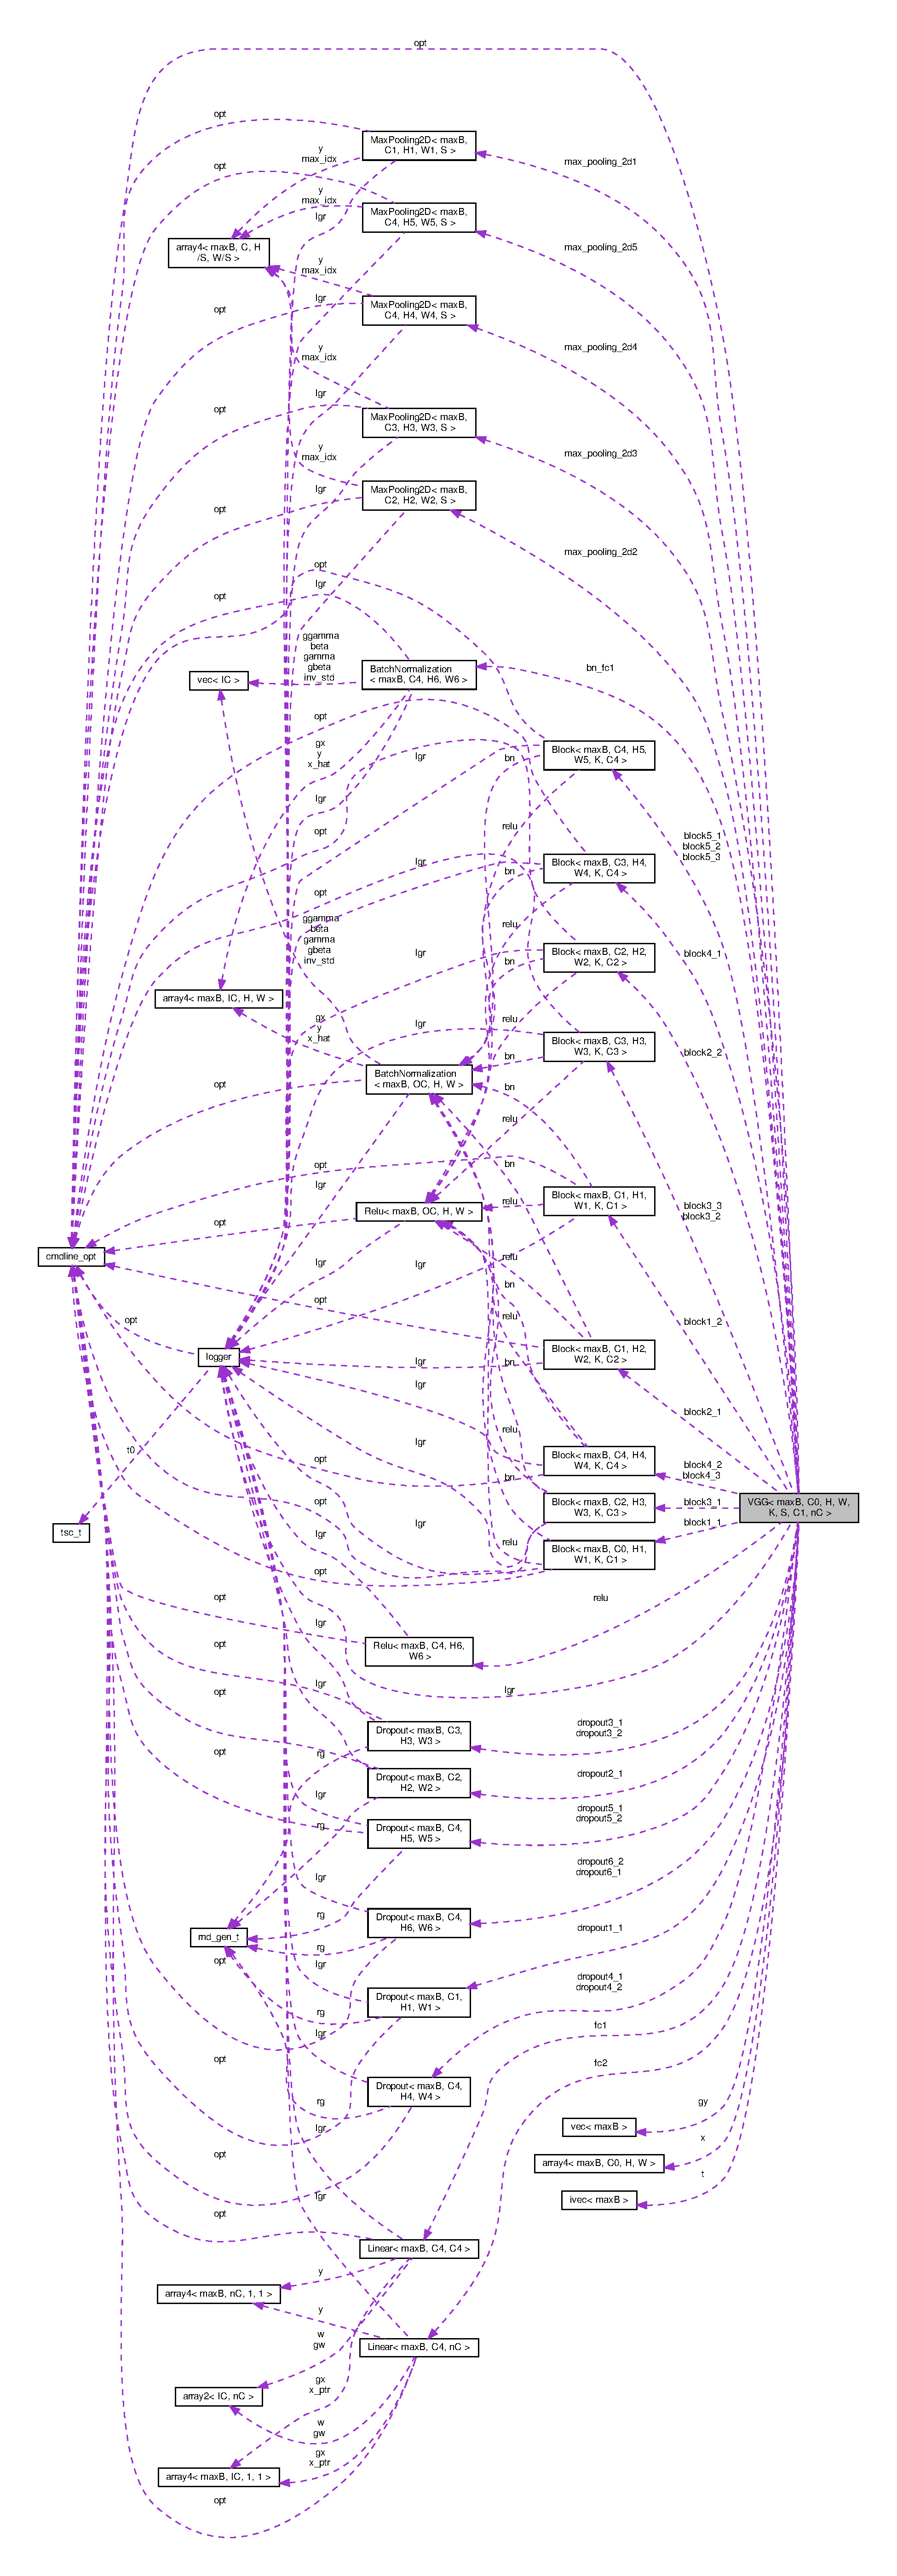
\includegraphics[height=550pt]{structVGG__coll__graph}
\end{center}
\end{figure}
\subsection*{Public Member Functions}
\begin{DoxyCompactItemize}
\item 
void \hyperlink{structVGG_aa8700968e0ee177cf7f129b2d46231fd}{init} (\hyperlink{structcmdline__opt}{cmdline\+\_\+opt} \hyperlink{structVGG_ad161d19c0d519768f32deca8dfd0598b}{opt}, \hyperlink{structlogger}{logger} $\ast$\hyperlink{structVGG_a5a8069856b54deb20f0b45e4522d9e4a}{lgr}, \hyperlink{structrnd__gen__t}{rnd\+\_\+gen\+\_\+t} \&rg)
\begin{DoxyCompactList}\small\item\em initialize \end{DoxyCompactList}\item 
\hyperlink{structVGG}{V\+GG}$<$ maxB, C0, H, W, K, S, C1, nC $>$ $\ast$ \hyperlink{structVGG_a671e3b02b9a8e55c274f7863a116af30}{copy} ()
\begin{DoxyCompactList}\small\item\em make a copy of this \end{DoxyCompactList}\item 
void \hyperlink{structVGG_a07e0570fe0eb7152dee4eff0c0bcc86f}{set\+\_\+dev} (\hyperlink{structVGG}{V\+GG}$<$ maxB, C0, H, W, K, S, C1, nC $>$ $\ast$\hyperlink{structVGG_acb66854790b4211ec6964690dcaba67b}{dev})
\begin{DoxyCompactList}\small\item\em set the device pointer for this and all subobjects \end{DoxyCompactList}\item 
void \hyperlink{structVGG_a26e977db7cff56b6bd9e2a8183635551}{make\+\_\+dev} ()
\begin{DoxyCompactList}\small\item\em if the algorithm is a gpu algorithm, allocate a device shadow of this object and set dev field of this and all subobjects. otherwise it sets all dev fields to null. \end{DoxyCompactList}\item 
void \hyperlink{structVGG_ab3bcd5bb62b66713f5bf0ba3c8b539cb}{del\+\_\+dev} ()
\begin{DoxyCompactList}\small\item\em if the algorithm is a gpu algorithm, dev field must not be null and deallocate it. \end{DoxyCompactList}\item 
\mbox{\Hypertarget{structVGG_a2f45518df66ff8196e3224367739b590}\label{structVGG_a2f45518df66ff8196e3224367739b590}} 
void \hyperlink{structVGG_a2f45518df66ff8196e3224367739b590}{to\+\_\+dev} ()
\begin{DoxyCompactList}\small\item\em if the algorithm is a gpu algorithm, dev field must not be null and send the host data to the device memory \end{DoxyCompactList}\item 
\mbox{\Hypertarget{structVGG_ac4ea480624b916204e717a4f8b3b9db1}\label{structVGG_ac4ea480624b916204e717a4f8b3b9db1}} 
void \hyperlink{structVGG_ac4ea480624b916204e717a4f8b3b9db1}{to\+\_\+host} ()
\begin{DoxyCompactList}\small\item\em if the algorithm is a gpu algorithm, dev field must not be null and send the device data to the host memory \end{DoxyCompactList}\item 
void \hyperlink{structVGG_a1adaccb289e6577317b49df5e1f3b465}{update} (\hyperlink{vgg__util_8h_a1082d08aaa761215ec83e7149f27ad16}{real} eta)
\begin{DoxyCompactList}\small\item\em update weights of all sublayers with gradients that must have been computed \end{DoxyCompactList}\item 
\hyperlink{structvec}{vec}$<$ maxB $>$ \& \hyperlink{structVGG_a256a1792818900ab2023554cea1ebb31}{forward} (\hyperlink{structarray4}{array4}$<$ maxB, C0, H, W $>$ \&\hyperlink{structVGG_ab352e8c1793b749d92b85e75ca4f66e8}{x}, \hyperlink{structivec}{ivec}$<$ maxB $>$ \&\hyperlink{structVGG_a302cf15e5bd6f920d527334df6f3e2b2}{t})
\begin{DoxyCompactList}\small\item\em calc the loss function of a mini-\/batch (x,t) \end{DoxyCompactList}\item 
\hyperlink{structarray4}{array4}$<$ maxB, C0, \hyperlink{structVGG_a73f189c70eef33b8e8de32929db37b10}{H1}, \hyperlink{structVGG_a01305ab6d90c95eb50c45352203b07e0}{W1} $>$ \& \hyperlink{structVGG_ad6c413558605836d7cffa87dc2971628}{backward} (\hyperlink{structvec}{vec}$<$ maxB $>$ \&\hyperlink{structVGG_a4a45e28a72f469b5b1432ee572627c17}{gy})
\begin{DoxyCompactList}\small\item\em calc the gradient of loss wrt the input (x) \end{DoxyCompactList}\item 
\hyperlink{vgg__util_8h_a1082d08aaa761215ec83e7149f27ad16}{real} \hyperlink{structVGG_a5a97c3db3635e480b1160ff24793feb6}{forward\+\_\+backward\+\_\+update} (\hyperlink{structarray4}{array4}$<$ maxB, C0, H, W $>$ \&\hyperlink{structVGG_ab352e8c1793b749d92b85e75ca4f66e8}{x}, \hyperlink{structivec}{ivec}$<$ maxB $>$ \&\hyperlink{structVGG_a302cf15e5bd6f920d527334df6f3e2b2}{t}, \hyperlink{vgg__util_8h_a1082d08aaa761215ec83e7149f27ad16}{real} eta)
\begin{DoxyCompactList}\small\item\em perform an entire iteration (= forward; backward; update) \end{DoxyCompactList}\item 
void \hyperlink{structVGG_a4dfe4a13d0b10b743acb1f2c7ed9cea9}{rand\+\_\+grad} (\hyperlink{structrnd__gen__t}{rnd\+\_\+gen\+\_\+t} \&rg, \hyperlink{vgg__util_8h_a1082d08aaa761215ec83e7149f27ad16}{real} p, \hyperlink{vgg__util_8h_a1082d08aaa761215ec83e7149f27ad16}{real} q)
\begin{DoxyCompactList}\small\item\em randomly set all gradients to values between p and q \end{DoxyCompactList}\item 
void \hyperlink{structVGG_a278f6bb4011563977a3965d592eb7ce8}{set\+\_\+grad} (\hyperlink{structVGG}{V\+GG}$<$ maxB, C0, H, W, K, S, C1, nC $>$ \&o)
\begin{DoxyCompactList}\small\item\em set all gradients to gradients of another object \end{DoxyCompactList}\item 
\hyperlink{vgg__util_8h_a1082d08aaa761215ec83e7149f27ad16}{real} \hyperlink{structVGG_a07fae8209634342bbc335be1b342b8c7}{gw\+\_\+dot\+\_\+gw} (\hyperlink{structVGG}{V\+GG}$<$ maxB, C0, H, W, K, S, C1, nC $>$ \&b)
\begin{DoxyCompactList}\small\item\em take the inner product of gradients \end{DoxyCompactList}\end{DoxyCompactItemize}
\subsection*{Public Attributes}
\begin{DoxyCompactItemize}
\item 
\hyperlink{structVGG}{V\+GG}$<$ maxB, C0, H, W, K, S, C1, nC $>$ $\ast$ \hyperlink{structVGG_acb66854790b4211ec6964690dcaba67b}{dev}
\item 
\hyperlink{structcmdline__opt}{cmdline\+\_\+opt} \hyperlink{structVGG_ad161d19c0d519768f32deca8dfd0598b}{opt}
\item 
\hyperlink{structlogger}{logger} $\ast$ \hyperlink{structVGG_a5a8069856b54deb20f0b45e4522d9e4a}{lgr}
\item 
\hyperlink{structarray4}{array4}$<$ maxB, C0, H, W $>$ \hyperlink{structVGG_ab352e8c1793b749d92b85e75ca4f66e8}{x}
\item 
\hyperlink{structivec}{ivec}$<$ maxB $>$ \hyperlink{structVGG_a302cf15e5bd6f920d527334df6f3e2b2}{t}
\item 
\hyperlink{structvec}{vec}$<$ maxB $>$ \hyperlink{structVGG_a4a45e28a72f469b5b1432ee572627c17}{gy}
\item 
\hyperlink{structBlock}{Block}$<$ maxB, C0, \hyperlink{structVGG_a73f189c70eef33b8e8de32929db37b10}{H1}, \hyperlink{structVGG_a01305ab6d90c95eb50c45352203b07e0}{W1}, K, C1 $>$ \hyperlink{structVGG_ac5d2224851fa2936be629e3fdf89c959}{block1\+\_\+1}
\item 
\hyperlink{structDropout}{Dropout}$<$ maxB, C1, \hyperlink{structVGG_a73f189c70eef33b8e8de32929db37b10}{H1}, \hyperlink{structVGG_a01305ab6d90c95eb50c45352203b07e0}{W1} $>$ \hyperlink{structVGG_ac98c33f424e29ec2e36fb4348586b4fd}{dropout1\+\_\+1}
\item 
\hyperlink{structBlock}{Block}$<$ maxB, C1, \hyperlink{structVGG_a73f189c70eef33b8e8de32929db37b10}{H1}, \hyperlink{structVGG_a01305ab6d90c95eb50c45352203b07e0}{W1}, K, C1 $>$ \hyperlink{structVGG_a8f6b6e4fa1009a0730e8ac7417ca4386}{block1\+\_\+2}
\item 
\hyperlink{structMaxPooling2D}{Max\+Pooling2D}$<$ maxB, C1, \hyperlink{structVGG_a73f189c70eef33b8e8de32929db37b10}{H1}, \hyperlink{structVGG_a01305ab6d90c95eb50c45352203b07e0}{W1}, S $>$ \hyperlink{structVGG_a065b2bedbdef89ba2943d696fb54da61}{max\+\_\+pooling\+\_\+2d1}
\item 
\hyperlink{structBlock}{Block}$<$ maxB, C1, \hyperlink{structVGG_a6658da7d5fd275b2af6eb75511ba6f80}{H2}, \hyperlink{structVGG_ac4a4d00b5e2ee41b1d4e8861bbc6c499}{W2}, K, \hyperlink{structVGG_a1e9ad0d15e42696798d44b06ad3c9a9a}{C2} $>$ \hyperlink{structVGG_a29cfe2459ad162095c5d420d12448de3}{block2\+\_\+1}
\item 
\hyperlink{structDropout}{Dropout}$<$ maxB, \hyperlink{structVGG_a1e9ad0d15e42696798d44b06ad3c9a9a}{C2}, \hyperlink{structVGG_a6658da7d5fd275b2af6eb75511ba6f80}{H2}, \hyperlink{structVGG_ac4a4d00b5e2ee41b1d4e8861bbc6c499}{W2} $>$ \hyperlink{structVGG_a691b281e14f4c2c17bcf2f5fa25b950d}{dropout2\+\_\+1}
\item 
\hyperlink{structBlock}{Block}$<$ maxB, \hyperlink{structVGG_a1e9ad0d15e42696798d44b06ad3c9a9a}{C2}, \hyperlink{structVGG_a6658da7d5fd275b2af6eb75511ba6f80}{H2}, \hyperlink{structVGG_ac4a4d00b5e2ee41b1d4e8861bbc6c499}{W2}, K, \hyperlink{structVGG_a1e9ad0d15e42696798d44b06ad3c9a9a}{C2} $>$ \hyperlink{structVGG_a421787324ebcaa4cc140c7eb588818df}{block2\+\_\+2}
\item 
\hyperlink{structMaxPooling2D}{Max\+Pooling2D}$<$ maxB, \hyperlink{structVGG_a1e9ad0d15e42696798d44b06ad3c9a9a}{C2}, \hyperlink{structVGG_a6658da7d5fd275b2af6eb75511ba6f80}{H2}, \hyperlink{structVGG_ac4a4d00b5e2ee41b1d4e8861bbc6c499}{W2}, S $>$ \hyperlink{structVGG_a2f4ff4efd026307976663ba43dd678c9}{max\+\_\+pooling\+\_\+2d2}
\item 
\hyperlink{structBlock}{Block}$<$ maxB, \hyperlink{structVGG_a1e9ad0d15e42696798d44b06ad3c9a9a}{C2}, \hyperlink{structVGG_aad221438514d3b1a829d7f9c27a6f5ea}{H3}, \hyperlink{structVGG_ad3bde49e961175621e0937584dae0af0}{W3}, K, \hyperlink{structVGG_a88a35c950ca73035ad75644925c05061}{C3} $>$ \hyperlink{structVGG_a89a31b1def0a1fad5f76e2a33ddf1489}{block3\+\_\+1}
\item 
\hyperlink{structDropout}{Dropout}$<$ maxB, \hyperlink{structVGG_a88a35c950ca73035ad75644925c05061}{C3}, \hyperlink{structVGG_aad221438514d3b1a829d7f9c27a6f5ea}{H3}, \hyperlink{structVGG_ad3bde49e961175621e0937584dae0af0}{W3} $>$ \hyperlink{structVGG_a3f8cb97bce4b3641088b8d33b151427d}{dropout3\+\_\+1}
\item 
\hyperlink{structBlock}{Block}$<$ maxB, \hyperlink{structVGG_a88a35c950ca73035ad75644925c05061}{C3}, \hyperlink{structVGG_aad221438514d3b1a829d7f9c27a6f5ea}{H3}, \hyperlink{structVGG_ad3bde49e961175621e0937584dae0af0}{W3}, K, \hyperlink{structVGG_a88a35c950ca73035ad75644925c05061}{C3} $>$ \hyperlink{structVGG_ae6f0d3f40c0c1f1f2fe656e446be7dd9}{block3\+\_\+2}
\item 
\hyperlink{structDropout}{Dropout}$<$ maxB, \hyperlink{structVGG_a88a35c950ca73035ad75644925c05061}{C3}, \hyperlink{structVGG_aad221438514d3b1a829d7f9c27a6f5ea}{H3}, \hyperlink{structVGG_ad3bde49e961175621e0937584dae0af0}{W3} $>$ \hyperlink{structVGG_ae6b26b5e9a686f3ff6be6c95a56363c1}{dropout3\+\_\+2}
\item 
\hyperlink{structBlock}{Block}$<$ maxB, \hyperlink{structVGG_a88a35c950ca73035ad75644925c05061}{C3}, \hyperlink{structVGG_aad221438514d3b1a829d7f9c27a6f5ea}{H3}, \hyperlink{structVGG_ad3bde49e961175621e0937584dae0af0}{W3}, K, \hyperlink{structVGG_a88a35c950ca73035ad75644925c05061}{C3} $>$ \hyperlink{structVGG_a8002c03bc72a210d6bba027abf770ee5}{block3\+\_\+3}
\item 
\hyperlink{structMaxPooling2D}{Max\+Pooling2D}$<$ maxB, \hyperlink{structVGG_a88a35c950ca73035ad75644925c05061}{C3}, \hyperlink{structVGG_aad221438514d3b1a829d7f9c27a6f5ea}{H3}, \hyperlink{structVGG_ad3bde49e961175621e0937584dae0af0}{W3}, S $>$ \hyperlink{structVGG_a0c29593e7a4726099dc2b982534df479}{max\+\_\+pooling\+\_\+2d3}
\item 
\hyperlink{structBlock}{Block}$<$ maxB, \hyperlink{structVGG_a88a35c950ca73035ad75644925c05061}{C3}, \hyperlink{structVGG_a1754afced5b0bbb91031179c1f58ee29}{H4}, \hyperlink{structVGG_a9728cd3ccfa5011d2a795dff7e9abfe8}{W4}, K, \hyperlink{structVGG_a4d54a1cc3e99340dfb67e7252719c663}{C4} $>$ \hyperlink{structVGG_a1461b736e9753f364a317c8e6305bb45}{block4\+\_\+1}
\item 
\hyperlink{structDropout}{Dropout}$<$ maxB, \hyperlink{structVGG_a4d54a1cc3e99340dfb67e7252719c663}{C4}, \hyperlink{structVGG_a1754afced5b0bbb91031179c1f58ee29}{H4}, \hyperlink{structVGG_a9728cd3ccfa5011d2a795dff7e9abfe8}{W4} $>$ \hyperlink{structVGG_ad0b64f61c99e5449686362dffcc9e5ff}{dropout4\+\_\+1}
\item 
\hyperlink{structBlock}{Block}$<$ maxB, \hyperlink{structVGG_a4d54a1cc3e99340dfb67e7252719c663}{C4}, \hyperlink{structVGG_a1754afced5b0bbb91031179c1f58ee29}{H4}, \hyperlink{structVGG_a9728cd3ccfa5011d2a795dff7e9abfe8}{W4}, K, \hyperlink{structVGG_a4d54a1cc3e99340dfb67e7252719c663}{C4} $>$ \hyperlink{structVGG_a449afed7008be198d32d2dfb3b9c32ff}{block4\+\_\+2}
\item 
\hyperlink{structDropout}{Dropout}$<$ maxB, \hyperlink{structVGG_a4d54a1cc3e99340dfb67e7252719c663}{C4}, \hyperlink{structVGG_a1754afced5b0bbb91031179c1f58ee29}{H4}, \hyperlink{structVGG_a9728cd3ccfa5011d2a795dff7e9abfe8}{W4} $>$ \hyperlink{structVGG_a2309b0f61c5f16e7bb8425ab813e80c6}{dropout4\+\_\+2}
\item 
\hyperlink{structBlock}{Block}$<$ maxB, \hyperlink{structVGG_a4d54a1cc3e99340dfb67e7252719c663}{C4}, \hyperlink{structVGG_a1754afced5b0bbb91031179c1f58ee29}{H4}, \hyperlink{structVGG_a9728cd3ccfa5011d2a795dff7e9abfe8}{W4}, K, \hyperlink{structVGG_a4d54a1cc3e99340dfb67e7252719c663}{C4} $>$ \hyperlink{structVGG_a67b4a234cca6e0ececd290de5ef13063}{block4\+\_\+3}
\item 
\hyperlink{structMaxPooling2D}{Max\+Pooling2D}$<$ maxB, \hyperlink{structVGG_a4d54a1cc3e99340dfb67e7252719c663}{C4}, \hyperlink{structVGG_a1754afced5b0bbb91031179c1f58ee29}{H4}, \hyperlink{structVGG_a9728cd3ccfa5011d2a795dff7e9abfe8}{W4}, S $>$ \hyperlink{structVGG_a0afbca6558a3efbad8a54c8d9c962d72}{max\+\_\+pooling\+\_\+2d4}
\item 
\hyperlink{structBlock}{Block}$<$ maxB, \hyperlink{structVGG_a4d54a1cc3e99340dfb67e7252719c663}{C4}, \hyperlink{structVGG_a763d01cce59fd355cbcfb7b09c3c8cdc}{H5}, \hyperlink{structVGG_a01d04c8b89719716a0c45c3631765875}{W5}, K, \hyperlink{structVGG_a4d54a1cc3e99340dfb67e7252719c663}{C4} $>$ \hyperlink{structVGG_ae2947bb7379eb4e5803854f25883304d}{block5\+\_\+1}
\item 
\hyperlink{structDropout}{Dropout}$<$ maxB, \hyperlink{structVGG_a4d54a1cc3e99340dfb67e7252719c663}{C4}, \hyperlink{structVGG_a763d01cce59fd355cbcfb7b09c3c8cdc}{H5}, \hyperlink{structVGG_a01d04c8b89719716a0c45c3631765875}{W5} $>$ \hyperlink{structVGG_ac70005cd3deace7f8d5d8101cc17d43c}{dropout5\+\_\+1}
\item 
\hyperlink{structBlock}{Block}$<$ maxB, \hyperlink{structVGG_a4d54a1cc3e99340dfb67e7252719c663}{C4}, \hyperlink{structVGG_a763d01cce59fd355cbcfb7b09c3c8cdc}{H5}, \hyperlink{structVGG_a01d04c8b89719716a0c45c3631765875}{W5}, K, \hyperlink{structVGG_a4d54a1cc3e99340dfb67e7252719c663}{C4} $>$ \hyperlink{structVGG_a6f7a1d645be0c7421d5808613a0a22bf}{block5\+\_\+2}
\item 
\hyperlink{structDropout}{Dropout}$<$ maxB, \hyperlink{structVGG_a4d54a1cc3e99340dfb67e7252719c663}{C4}, \hyperlink{structVGG_a763d01cce59fd355cbcfb7b09c3c8cdc}{H5}, \hyperlink{structVGG_a01d04c8b89719716a0c45c3631765875}{W5} $>$ \hyperlink{structVGG_a10005c43661e059cfebc8e004e7bc344}{dropout5\+\_\+2}
\item 
\hyperlink{structBlock}{Block}$<$ maxB, \hyperlink{structVGG_a4d54a1cc3e99340dfb67e7252719c663}{C4}, \hyperlink{structVGG_a763d01cce59fd355cbcfb7b09c3c8cdc}{H5}, \hyperlink{structVGG_a01d04c8b89719716a0c45c3631765875}{W5}, K, \hyperlink{structVGG_a4d54a1cc3e99340dfb67e7252719c663}{C4} $>$ \hyperlink{structVGG_a8a6bf842367d6269c6e0bd40e06115f2}{block5\+\_\+3}
\item 
\hyperlink{structMaxPooling2D}{Max\+Pooling2D}$<$ maxB, \hyperlink{structVGG_a4d54a1cc3e99340dfb67e7252719c663}{C4}, \hyperlink{structVGG_a763d01cce59fd355cbcfb7b09c3c8cdc}{H5}, \hyperlink{structVGG_a01d04c8b89719716a0c45c3631765875}{W5}, S $>$ \hyperlink{structVGG_a71a381756e7f6f60347d99d05b3f0b1a}{max\+\_\+pooling\+\_\+2d5}
\item 
\hyperlink{structDropout}{Dropout}$<$ maxB, \hyperlink{structVGG_a4d54a1cc3e99340dfb67e7252719c663}{C4}, \hyperlink{structVGG_aca7e136480c1e76d74bda917c1ddca97}{H6}, \hyperlink{structVGG_ada7bec62e12fac368b103ae3d8c59c0e}{W6} $>$ \hyperlink{structVGG_a3ed68e318387ff7e87b1c0d957d8d24a}{dropout6\+\_\+1}
\item 
\hyperlink{structLinear}{Linear}$<$ maxB, \hyperlink{structVGG_a4d54a1cc3e99340dfb67e7252719c663}{C4}, \hyperlink{structVGG_a4d54a1cc3e99340dfb67e7252719c663}{C4} $>$ \hyperlink{structVGG_aca67ef058fa46d4f74022f308c72ad6c}{fc1}
\item 
\hyperlink{structBatchNormalization}{Batch\+Normalization}$<$ maxB, \hyperlink{structVGG_a4d54a1cc3e99340dfb67e7252719c663}{C4}, \hyperlink{structVGG_aca7e136480c1e76d74bda917c1ddca97}{H6}, \hyperlink{structVGG_ada7bec62e12fac368b103ae3d8c59c0e}{W6} $>$ \hyperlink{structVGG_a6a98e7662114881d493b635ca57fbf28}{bn\+\_\+fc1}
\item 
\hyperlink{structRelu}{Relu}$<$ maxB, \hyperlink{structVGG_a4d54a1cc3e99340dfb67e7252719c663}{C4}, \hyperlink{structVGG_aca7e136480c1e76d74bda917c1ddca97}{H6}, \hyperlink{structVGG_ada7bec62e12fac368b103ae3d8c59c0e}{W6} $>$ \hyperlink{structVGG_acc01c963dd716345709ab91f5eb6e2e3}{relu}
\item 
\hyperlink{structDropout}{Dropout}$<$ maxB, \hyperlink{structVGG_a4d54a1cc3e99340dfb67e7252719c663}{C4}, \hyperlink{structVGG_aca7e136480c1e76d74bda917c1ddca97}{H6}, \hyperlink{structVGG_ada7bec62e12fac368b103ae3d8c59c0e}{W6} $>$ \hyperlink{structVGG_abecd584b5b4bf336077b181e4f3e6f50}{dropout6\+\_\+2}
\item 
\hyperlink{structLinear}{Linear}$<$ maxB, \hyperlink{structVGG_a4d54a1cc3e99340dfb67e7252719c663}{C4}, nC $>$ \hyperlink{structVGG_a422a4d5100d100bb361155b1f093ebf7}{fc2}
\item 
\hyperlink{structSoftmaxCrossEntropy}{Softmax\+Cross\+Entropy}$<$ maxB, nC $>$ \hyperlink{structVGG_af4bbc09cef74dbbff99b5a35f2c40608}{softmax\+\_\+cross\+\_\+entropy}
\end{DoxyCompactItemize}
\subsection*{Static Public Attributes}
\begin{DoxyCompactItemize}
\item 
static const \hyperlink{vgg__util_8h_a8e93478a00e685bea5e6a3f617bf03a3}{idx\+\_\+t} \hyperlink{structVGG_a73f189c70eef33b8e8de32929db37b10}{H1} = H
\item 
static const \hyperlink{vgg__util_8h_a8e93478a00e685bea5e6a3f617bf03a3}{idx\+\_\+t} \hyperlink{structVGG_a01305ab6d90c95eb50c45352203b07e0}{W1} = W
\item 
static const \hyperlink{vgg__util_8h_a8e93478a00e685bea5e6a3f617bf03a3}{idx\+\_\+t} \hyperlink{structVGG_a6658da7d5fd275b2af6eb75511ba6f80}{H2} = H/S
\item 
static const \hyperlink{vgg__util_8h_a8e93478a00e685bea5e6a3f617bf03a3}{idx\+\_\+t} \hyperlink{structVGG_ac4a4d00b5e2ee41b1d4e8861bbc6c499}{W2} = W/S
\item 
static const \hyperlink{vgg__util_8h_a8e93478a00e685bea5e6a3f617bf03a3}{idx\+\_\+t} \hyperlink{structVGG_a1e9ad0d15e42696798d44b06ad3c9a9a}{C2} = S$\ast$C1
\item 
static const \hyperlink{vgg__util_8h_a8e93478a00e685bea5e6a3f617bf03a3}{idx\+\_\+t} \hyperlink{structVGG_aad221438514d3b1a829d7f9c27a6f5ea}{H3} = \hyperlink{structVGG_a6658da7d5fd275b2af6eb75511ba6f80}{H2}/S
\item 
static const \hyperlink{vgg__util_8h_a8e93478a00e685bea5e6a3f617bf03a3}{idx\+\_\+t} \hyperlink{structVGG_ad3bde49e961175621e0937584dae0af0}{W3} = \hyperlink{structVGG_ac4a4d00b5e2ee41b1d4e8861bbc6c499}{W2}/S
\item 
static const \hyperlink{vgg__util_8h_a8e93478a00e685bea5e6a3f617bf03a3}{idx\+\_\+t} \hyperlink{structVGG_a88a35c950ca73035ad75644925c05061}{C3} = S$\ast$\hyperlink{structVGG_a1e9ad0d15e42696798d44b06ad3c9a9a}{C2}
\item 
static const \hyperlink{vgg__util_8h_a8e93478a00e685bea5e6a3f617bf03a3}{idx\+\_\+t} \hyperlink{structVGG_a1754afced5b0bbb91031179c1f58ee29}{H4} = \hyperlink{structVGG_aad221438514d3b1a829d7f9c27a6f5ea}{H3}/S
\item 
static const \hyperlink{vgg__util_8h_a8e93478a00e685bea5e6a3f617bf03a3}{idx\+\_\+t} \hyperlink{structVGG_a9728cd3ccfa5011d2a795dff7e9abfe8}{W4} = \hyperlink{structVGG_ad3bde49e961175621e0937584dae0af0}{W3}/S
\item 
static const \hyperlink{vgg__util_8h_a8e93478a00e685bea5e6a3f617bf03a3}{idx\+\_\+t} \hyperlink{structVGG_a4d54a1cc3e99340dfb67e7252719c663}{C4} = S$\ast$\hyperlink{structVGG_a88a35c950ca73035ad75644925c05061}{C3}
\item 
static const \hyperlink{vgg__util_8h_a8e93478a00e685bea5e6a3f617bf03a3}{idx\+\_\+t} \hyperlink{structVGG_a763d01cce59fd355cbcfb7b09c3c8cdc}{H5} = \hyperlink{structVGG_a1754afced5b0bbb91031179c1f58ee29}{H4}/S
\item 
static const \hyperlink{vgg__util_8h_a8e93478a00e685bea5e6a3f617bf03a3}{idx\+\_\+t} \hyperlink{structVGG_a01d04c8b89719716a0c45c3631765875}{W5} = \hyperlink{structVGG_a9728cd3ccfa5011d2a795dff7e9abfe8}{W4}/S
\item 
static const \hyperlink{vgg__util_8h_a8e93478a00e685bea5e6a3f617bf03a3}{idx\+\_\+t} \hyperlink{structVGG_aca7e136480c1e76d74bda917c1ddca97}{H6} = \hyperlink{structVGG_a763d01cce59fd355cbcfb7b09c3c8cdc}{H5}/S
\item 
static const \hyperlink{vgg__util_8h_a8e93478a00e685bea5e6a3f617bf03a3}{idx\+\_\+t} \hyperlink{structVGG_ada7bec62e12fac368b103ae3d8c59c0e}{W6} = \hyperlink{structVGG_a01d04c8b89719716a0c45c3631765875}{W5}/S
\end{DoxyCompactItemize}


\subsection{Detailed Description}
\subsubsection*{template$<$idx\+\_\+t maxB, idx\+\_\+t C0, idx\+\_\+t H, idx\+\_\+t W, idx\+\_\+t K, idx\+\_\+t S, idx\+\_\+t C1, idx\+\_\+t nC$>$\newline
struct V\+G\+G$<$ max\+B, C0, H, W, K, S, C1, n\+C $>$}

\hyperlink{structVGG}{V\+GG} network. 


\begin{DoxyParams}{Parameters}
{\em (max\+B)} & maximum batch size it can accommodate (64) \\
\hline
{\em (\+C0)} & the number of channels in an input image (3) \\
\hline
{\em (\+H)} & height of an input image (32) \\
\hline
{\em (\+W)} & width of an input image (32) \\
\hline
{\em (\+K)} & convolution kernel size (1). filter array has (2\+K+1)$\ast$(2\+K+1) elems) \\
\hline
{\em (\+S)} & shrink factor of pooling layers (2) \\
\hline
{\em (\+C1)} & number of channels in the first hidden layer (64). those in the following layers are C1/2, C2/4, C3/8, ..., 1 \\
\hline
{\em (n\+C)} & number of classes (10) \\
\hline
\end{DoxyParams}


\subsection{Member Function Documentation}
\mbox{\Hypertarget{structVGG_ad6c413558605836d7cffa87dc2971628}\label{structVGG_ad6c413558605836d7cffa87dc2971628}} 
\index{V\+GG@{V\+GG}!backward@{backward}}
\index{backward@{backward}!V\+GG@{V\+GG}}
\subsubsection{\texorpdfstring{backward()}{backward()}}
{\footnotesize\ttfamily template$<$idx\+\_\+t maxB, idx\+\_\+t C0, idx\+\_\+t H, idx\+\_\+t W, idx\+\_\+t K, idx\+\_\+t S, idx\+\_\+t C1, idx\+\_\+t nC$>$ \\
\hyperlink{structarray4}{array4}$<$maxB,C0,\hyperlink{structVGG_a73f189c70eef33b8e8de32929db37b10}{H1},\hyperlink{structVGG_a01305ab6d90c95eb50c45352203b07e0}{W1}$>$\& \hyperlink{structVGG}{V\+GG}$<$ maxB, C0, H, W, K, S, C1, nC $>$\+::backward (\begin{DoxyParamCaption}\item[{\hyperlink{structvec}{vec}$<$ maxB $>$ \&}]{gy }\end{DoxyParamCaption})\hspace{0.3cm}{\ttfamily [inline]}}



calc the gradient of loss wrt the input (x) 


\begin{DoxyParams}{Parameters}
{\em (gy)} & gradient of loss with respect to the output\\
\hline
\end{DoxyParams}
calc the gradient of loss wrt the input. along the way, it also calculates the gradient of loss wrt weights for all sublayers that have weights. since this is the entire network, gy is actually a vector whose components are all 1. (loss = sum of losses of each data). \begin{DoxySeeAlso}{See also}
\hyperlink{structVGG_a256a1792818900ab2023554cea1ebb31}{forward} 

\hyperlink{structVGG_a1adaccb289e6577317b49df5e1f3b465}{update} 
\end{DoxySeeAlso}
\mbox{\Hypertarget{structVGG_a671e3b02b9a8e55c274f7863a116af30}\label{structVGG_a671e3b02b9a8e55c274f7863a116af30}} 
\index{V\+GG@{V\+GG}!copy@{copy}}
\index{copy@{copy}!V\+GG@{V\+GG}}
\subsubsection{\texorpdfstring{copy()}{copy()}}
{\footnotesize\ttfamily template$<$idx\+\_\+t maxB, idx\+\_\+t C0, idx\+\_\+t H, idx\+\_\+t W, idx\+\_\+t K, idx\+\_\+t S, idx\+\_\+t C1, idx\+\_\+t nC$>$ \\
\hyperlink{structVGG}{V\+GG}$<$maxB,C0,H,W,K,S,C1,nC$>$$\ast$ \hyperlink{structVGG}{V\+GG}$<$ maxB, C0, H, W, K, S, C1, nC $>$\+::copy (\begin{DoxyParamCaption}{ }\end{DoxyParamCaption})\hspace{0.3cm}{\ttfamily [inline]}}



make a copy of this 

if this object has a device pointer, the copy will have a device pointer too, but its contents are N\+OT copied \mbox{\Hypertarget{structVGG_ab3bcd5bb62b66713f5bf0ba3c8b539cb}\label{structVGG_ab3bcd5bb62b66713f5bf0ba3c8b539cb}} 
\index{V\+GG@{V\+GG}!del\+\_\+dev@{del\+\_\+dev}}
\index{del\+\_\+dev@{del\+\_\+dev}!V\+GG@{V\+GG}}
\subsubsection{\texorpdfstring{del\+\_\+dev()}{del\_dev()}}
{\footnotesize\ttfamily template$<$idx\+\_\+t maxB, idx\+\_\+t C0, idx\+\_\+t H, idx\+\_\+t W, idx\+\_\+t K, idx\+\_\+t S, idx\+\_\+t C1, idx\+\_\+t nC$>$ \\
void \hyperlink{structVGG}{V\+GG}$<$ maxB, C0, H, W, K, S, C1, nC $>$\+::del\+\_\+dev (\begin{DoxyParamCaption}{ }\end{DoxyParamCaption})\hspace{0.3cm}{\ttfamily [inline]}}



if the algorithm is a gpu algorithm, dev field must not be null and deallocate it. 

\begin{DoxySeeAlso}{See also}
\hyperlink{structVGG_a26e977db7cff56b6bd9e2a8183635551}{make\+\_\+dev} 

\hyperlink{structVGG_a07e0570fe0eb7152dee4eff0c0bcc86f}{set\+\_\+dev} 
\end{DoxySeeAlso}
\mbox{\Hypertarget{structVGG_a256a1792818900ab2023554cea1ebb31}\label{structVGG_a256a1792818900ab2023554cea1ebb31}} 
\index{V\+GG@{V\+GG}!forward@{forward}}
\index{forward@{forward}!V\+GG@{V\+GG}}
\subsubsection{\texorpdfstring{forward()}{forward()}}
{\footnotesize\ttfamily template$<$idx\+\_\+t maxB, idx\+\_\+t C0, idx\+\_\+t H, idx\+\_\+t W, idx\+\_\+t K, idx\+\_\+t S, idx\+\_\+t C1, idx\+\_\+t nC$>$ \\
\hyperlink{structvec}{vec}$<$maxB$>$\& \hyperlink{structVGG}{V\+GG}$<$ maxB, C0, H, W, K, S, C1, nC $>$\+::forward (\begin{DoxyParamCaption}\item[{\hyperlink{structarray4}{array4}$<$ maxB, C0, H, W $>$ \&}]{x,  }\item[{\hyperlink{structivec}{ivec}$<$ maxB $>$ \&}]{t }\end{DoxyParamCaption})\hspace{0.3cm}{\ttfamily [inline]}}



calc the loss function of a mini-\/batch (x,t) 


\begin{DoxyParams}{Parameters}
{\em (x)} & input images \\
\hline
{\em (t)} & true labels of images \\
\hline
\end{DoxyParams}
\begin{DoxySeeAlso}{See also}
\hyperlink{structVGG_ad6c413558605836d7cffa87dc2971628}{backward} 

\hyperlink{structVGG_a1adaccb289e6577317b49df5e1f3b465}{update} 
\end{DoxySeeAlso}
\mbox{\Hypertarget{structVGG_a5a97c3db3635e480b1160ff24793feb6}\label{structVGG_a5a97c3db3635e480b1160ff24793feb6}} 
\index{V\+GG@{V\+GG}!forward\+\_\+backward\+\_\+update@{forward\+\_\+backward\+\_\+update}}
\index{forward\+\_\+backward\+\_\+update@{forward\+\_\+backward\+\_\+update}!V\+GG@{V\+GG}}
\subsubsection{\texorpdfstring{forward\+\_\+backward\+\_\+update()}{forward\_backward\_update()}}
{\footnotesize\ttfamily template$<$idx\+\_\+t maxB, idx\+\_\+t C0, idx\+\_\+t H, idx\+\_\+t W, idx\+\_\+t K, idx\+\_\+t S, idx\+\_\+t C1, idx\+\_\+t nC$>$ \\
\hyperlink{vgg__util_8h_a1082d08aaa761215ec83e7149f27ad16}{real} \hyperlink{structVGG}{V\+GG}$<$ maxB, C0, H, W, K, S, C1, nC $>$\+::forward\+\_\+backward\+\_\+update (\begin{DoxyParamCaption}\item[{\hyperlink{structarray4}{array4}$<$ maxB, C0, H, W $>$ \&}]{x,  }\item[{\hyperlink{structivec}{ivec}$<$ maxB $>$ \&}]{t,  }\item[{\hyperlink{vgg__util_8h_a1082d08aaa761215ec83e7149f27ad16}{real}}]{eta }\end{DoxyParamCaption})\hspace{0.3cm}{\ttfamily [inline]}}



perform an entire iteration (= forward; backward; update) 


\begin{DoxyParams}{Parameters}
{\em (x)} & input images (a mini batch) \\
\hline
{\em (t)} & true labels \\
\hline
{\em (eta)} & learning rate \\
\hline
\end{DoxyParams}
\begin{DoxySeeAlso}{See also}
\hyperlink{structVGG_a256a1792818900ab2023554cea1ebb31}{forward} 

\hyperlink{structVGG_ad6c413558605836d7cffa87dc2971628}{backward} 

\hyperlink{structVGG_a1adaccb289e6577317b49df5e1f3b465}{update}
\end{DoxySeeAlso}
do everything on a mini-\/batch. forward calculates the loss wrt x and t; backward calculates the gradient of loss wrt x and weights; update updates weights with the gradients and the learning rate. \mbox{\Hypertarget{structVGG_a07fae8209634342bbc335be1b342b8c7}\label{structVGG_a07fae8209634342bbc335be1b342b8c7}} 
\index{V\+GG@{V\+GG}!gw\+\_\+dot\+\_\+gw@{gw\+\_\+dot\+\_\+gw}}
\index{gw\+\_\+dot\+\_\+gw@{gw\+\_\+dot\+\_\+gw}!V\+GG@{V\+GG}}
\subsubsection{\texorpdfstring{gw\+\_\+dot\+\_\+gw()}{gw\_dot\_gw()}}
{\footnotesize\ttfamily template$<$idx\+\_\+t maxB, idx\+\_\+t C0, idx\+\_\+t H, idx\+\_\+t W, idx\+\_\+t K, idx\+\_\+t S, idx\+\_\+t C1, idx\+\_\+t nC$>$ \\
\hyperlink{vgg__util_8h_a1082d08aaa761215ec83e7149f27ad16}{real} \hyperlink{structVGG}{V\+GG}$<$ maxB, C0, H, W, K, S, C1, nC $>$\+::gw\+\_\+dot\+\_\+gw (\begin{DoxyParamCaption}\item[{\hyperlink{structVGG}{V\+GG}$<$ maxB, C0, H, W, K, S, C1, nC $>$ \&}]{b }\end{DoxyParamCaption})\hspace{0.3cm}{\ttfamily [inline]}}



take the inner product of gradients 


\begin{DoxyParams}{Parameters}
{\em (b)} & the object to take the inner product with\\
\hline
\end{DoxyParams}
take the inner product of this object\textquotesingle{}s gradients and b\textquotesingle{}s gradients \mbox{\Hypertarget{structVGG_aa8700968e0ee177cf7f129b2d46231fd}\label{structVGG_aa8700968e0ee177cf7f129b2d46231fd}} 
\index{V\+GG@{V\+GG}!init@{init}}
\index{init@{init}!V\+GG@{V\+GG}}
\subsubsection{\texorpdfstring{init()}{init()}}
{\footnotesize\ttfamily template$<$idx\+\_\+t maxB, idx\+\_\+t C0, idx\+\_\+t H, idx\+\_\+t W, idx\+\_\+t K, idx\+\_\+t S, idx\+\_\+t C1, idx\+\_\+t nC$>$ \\
void \hyperlink{structVGG}{V\+GG}$<$ maxB, C0, H, W, K, S, C1, nC $>$\+::init (\begin{DoxyParamCaption}\item[{\hyperlink{structcmdline__opt}{cmdline\+\_\+opt}}]{opt,  }\item[{\hyperlink{structlogger}{logger} $\ast$}]{lgr,  }\item[{\hyperlink{structrnd__gen__t}{rnd\+\_\+gen\+\_\+t} \&}]{rg }\end{DoxyParamCaption})\hspace{0.3cm}{\ttfamily [inline]}}



initialize 


\begin{DoxyParams}{Parameters}
{\em (opt)} & command line options \\
\hline
{\em (lgr)} & logger \\
\hline
{\em (rg)} & random number generator for initializing weights \\
\hline
\end{DoxyParams}
\mbox{\Hypertarget{structVGG_a26e977db7cff56b6bd9e2a8183635551}\label{structVGG_a26e977db7cff56b6bd9e2a8183635551}} 
\index{V\+GG@{V\+GG}!make\+\_\+dev@{make\+\_\+dev}}
\index{make\+\_\+dev@{make\+\_\+dev}!V\+GG@{V\+GG}}
\subsubsection{\texorpdfstring{make\+\_\+dev()}{make\_dev()}}
{\footnotesize\ttfamily template$<$idx\+\_\+t maxB, idx\+\_\+t C0, idx\+\_\+t H, idx\+\_\+t W, idx\+\_\+t K, idx\+\_\+t S, idx\+\_\+t C1, idx\+\_\+t nC$>$ \\
void \hyperlink{structVGG}{V\+GG}$<$ maxB, C0, H, W, K, S, C1, nC $>$\+::make\+\_\+dev (\begin{DoxyParamCaption}{ }\end{DoxyParamCaption})\hspace{0.3cm}{\ttfamily [inline]}}



if the algorithm is a gpu algorithm, allocate a device shadow of this object and set dev field of this and all subobjects. otherwise it sets all dev fields to null. 

\begin{DoxySeeAlso}{See also}
\hyperlink{structVGG_a07e0570fe0eb7152dee4eff0c0bcc86f}{set\+\_\+dev} 

\hyperlink{structVGG_ab3bcd5bb62b66713f5bf0ba3c8b539cb}{del\+\_\+dev} 
\end{DoxySeeAlso}
\mbox{\Hypertarget{structVGG_a4dfe4a13d0b10b743acb1f2c7ed9cea9}\label{structVGG_a4dfe4a13d0b10b743acb1f2c7ed9cea9}} 
\index{V\+GG@{V\+GG}!rand\+\_\+grad@{rand\+\_\+grad}}
\index{rand\+\_\+grad@{rand\+\_\+grad}!V\+GG@{V\+GG}}
\subsubsection{\texorpdfstring{rand\+\_\+grad()}{rand\_grad()}}
{\footnotesize\ttfamily template$<$idx\+\_\+t maxB, idx\+\_\+t C0, idx\+\_\+t H, idx\+\_\+t W, idx\+\_\+t K, idx\+\_\+t S, idx\+\_\+t C1, idx\+\_\+t nC$>$ \\
void \hyperlink{structVGG}{V\+GG}$<$ maxB, C0, H, W, K, S, C1, nC $>$\+::rand\+\_\+grad (\begin{DoxyParamCaption}\item[{\hyperlink{structrnd__gen__t}{rnd\+\_\+gen\+\_\+t} \&}]{rg,  }\item[{\hyperlink{vgg__util_8h_a1082d08aaa761215ec83e7149f27ad16}{real}}]{p,  }\item[{\hyperlink{vgg__util_8h_a1082d08aaa761215ec83e7149f27ad16}{real}}]{q }\end{DoxyParamCaption})\hspace{0.3cm}{\ttfamily [inline]}}



randomly set all gradients to values between p and q 


\begin{DoxyParams}{Parameters}
{\em (rg)} & random number generator \\
\hline
{\em (p)} & minimum value of a component \\
\hline
{\em (q)} & maximum value of a component \\
\hline
\end{DoxyParams}
\mbox{\Hypertarget{structVGG_a07e0570fe0eb7152dee4eff0c0bcc86f}\label{structVGG_a07e0570fe0eb7152dee4eff0c0bcc86f}} 
\index{V\+GG@{V\+GG}!set\+\_\+dev@{set\+\_\+dev}}
\index{set\+\_\+dev@{set\+\_\+dev}!V\+GG@{V\+GG}}
\subsubsection{\texorpdfstring{set\+\_\+dev()}{set\_dev()}}
{\footnotesize\ttfamily template$<$idx\+\_\+t maxB, idx\+\_\+t C0, idx\+\_\+t H, idx\+\_\+t W, idx\+\_\+t K, idx\+\_\+t S, idx\+\_\+t C1, idx\+\_\+t nC$>$ \\
void \hyperlink{structVGG}{V\+GG}$<$ maxB, C0, H, W, K, S, C1, nC $>$\+::set\+\_\+dev (\begin{DoxyParamCaption}\item[{\hyperlink{structVGG}{V\+GG}$<$ maxB, C0, H, W, K, S, C1, nC $>$ $\ast$}]{dev }\end{DoxyParamCaption})\hspace{0.3cm}{\ttfamily [inline]}}



set the device pointer for this and all subobjects 


\begin{DoxyParams}{Parameters}
{\em (dev)} & a device memory or null \\
\hline
\end{DoxyParams}
\begin{DoxySeeAlso}{See also}
\hyperlink{structVGG_a26e977db7cff56b6bd9e2a8183635551}{make\+\_\+dev} 

\hyperlink{structVGG_ab3bcd5bb62b66713f5bf0ba3c8b539cb}{del\+\_\+dev}
\end{DoxySeeAlso}
if dev is not null, dev fields of all subojects point to the corresponding subjects in the device memory. if dev is not null, all dev fields become null. \mbox{\Hypertarget{structVGG_a278f6bb4011563977a3965d592eb7ce8}\label{structVGG_a278f6bb4011563977a3965d592eb7ce8}} 
\index{V\+GG@{V\+GG}!set\+\_\+grad@{set\+\_\+grad}}
\index{set\+\_\+grad@{set\+\_\+grad}!V\+GG@{V\+GG}}
\subsubsection{\texorpdfstring{set\+\_\+grad()}{set\_grad()}}
{\footnotesize\ttfamily template$<$idx\+\_\+t maxB, idx\+\_\+t C0, idx\+\_\+t H, idx\+\_\+t W, idx\+\_\+t K, idx\+\_\+t S, idx\+\_\+t C1, idx\+\_\+t nC$>$ \\
void \hyperlink{structVGG}{V\+GG}$<$ maxB, C0, H, W, K, S, C1, nC $>$\+::set\+\_\+grad (\begin{DoxyParamCaption}\item[{\hyperlink{structVGG}{V\+GG}$<$ maxB, C0, H, W, K, S, C1, nC $>$ \&}]{o }\end{DoxyParamCaption})\hspace{0.3cm}{\ttfamily [inline]}}



set all gradients to gradients of another object 


\begin{DoxyParams}{Parameters}
{\em (o)} & the object from which gradients get copied\\
\hline
\end{DoxyParams}
transfer gradients of o to this object \mbox{\Hypertarget{structVGG_a1adaccb289e6577317b49df5e1f3b465}\label{structVGG_a1adaccb289e6577317b49df5e1f3b465}} 
\index{V\+GG@{V\+GG}!update@{update}}
\index{update@{update}!V\+GG@{V\+GG}}
\subsubsection{\texorpdfstring{update()}{update()}}
{\footnotesize\ttfamily template$<$idx\+\_\+t maxB, idx\+\_\+t C0, idx\+\_\+t H, idx\+\_\+t W, idx\+\_\+t K, idx\+\_\+t S, idx\+\_\+t C1, idx\+\_\+t nC$>$ \\
void \hyperlink{structVGG}{V\+GG}$<$ maxB, C0, H, W, K, S, C1, nC $>$\+::update (\begin{DoxyParamCaption}\item[{\hyperlink{vgg__util_8h_a1082d08aaa761215ec83e7149f27ad16}{real}}]{eta }\end{DoxyParamCaption})\hspace{0.3cm}{\ttfamily [inline]}}



update weights of all sublayers with gradients that must have been computed 


\begin{DoxyParams}{Parameters}
{\em (eta)} & the learning rate \\
\hline
\end{DoxyParams}
\begin{DoxySeeAlso}{See also}
\hyperlink{structVGG_a256a1792818900ab2023554cea1ebb31}{forward} 

\hyperlink{structVGG_ad6c413558605836d7cffa87dc2971628}{backward} 
\end{DoxySeeAlso}


\subsection{Member Data Documentation}
\mbox{\Hypertarget{structVGG_ac5d2224851fa2936be629e3fdf89c959}\label{structVGG_ac5d2224851fa2936be629e3fdf89c959}} 
\index{V\+GG@{V\+GG}!block1\+\_\+1@{block1\+\_\+1}}
\index{block1\+\_\+1@{block1\+\_\+1}!V\+GG@{V\+GG}}
\subsubsection{\texorpdfstring{block1\+\_\+1}{block1\_1}}
{\footnotesize\ttfamily template$<$idx\+\_\+t maxB, idx\+\_\+t C0, idx\+\_\+t H, idx\+\_\+t W, idx\+\_\+t K, idx\+\_\+t S, idx\+\_\+t C1, idx\+\_\+t nC$>$ \\
\hyperlink{structBlock}{Block}$<$maxB,C0,\hyperlink{structVGG_a73f189c70eef33b8e8de32929db37b10}{H1},\hyperlink{structVGG_a01305ab6d90c95eb50c45352203b07e0}{W1},K,C1$>$ \hyperlink{structVGG}{V\+GG}$<$ maxB, C0, H, W, K, S, C1, nC $>$\+::block1\+\_\+1}

sublayer \mbox{\Hypertarget{structVGG_a8f6b6e4fa1009a0730e8ac7417ca4386}\label{structVGG_a8f6b6e4fa1009a0730e8ac7417ca4386}} 
\index{V\+GG@{V\+GG}!block1\+\_\+2@{block1\+\_\+2}}
\index{block1\+\_\+2@{block1\+\_\+2}!V\+GG@{V\+GG}}
\subsubsection{\texorpdfstring{block1\+\_\+2}{block1\_2}}
{\footnotesize\ttfamily template$<$idx\+\_\+t maxB, idx\+\_\+t C0, idx\+\_\+t H, idx\+\_\+t W, idx\+\_\+t K, idx\+\_\+t S, idx\+\_\+t C1, idx\+\_\+t nC$>$ \\
\hyperlink{structBlock}{Block}$<$maxB,C1,\hyperlink{structVGG_a73f189c70eef33b8e8de32929db37b10}{H1},\hyperlink{structVGG_a01305ab6d90c95eb50c45352203b07e0}{W1},K,C1$>$ \hyperlink{structVGG}{V\+GG}$<$ maxB, C0, H, W, K, S, C1, nC $>$\+::block1\+\_\+2}

sublayer \mbox{\Hypertarget{structVGG_a29cfe2459ad162095c5d420d12448de3}\label{structVGG_a29cfe2459ad162095c5d420d12448de3}} 
\index{V\+GG@{V\+GG}!block2\+\_\+1@{block2\+\_\+1}}
\index{block2\+\_\+1@{block2\+\_\+1}!V\+GG@{V\+GG}}
\subsubsection{\texorpdfstring{block2\+\_\+1}{block2\_1}}
{\footnotesize\ttfamily template$<$idx\+\_\+t maxB, idx\+\_\+t C0, idx\+\_\+t H, idx\+\_\+t W, idx\+\_\+t K, idx\+\_\+t S, idx\+\_\+t C1, idx\+\_\+t nC$>$ \\
\hyperlink{structBlock}{Block}$<$maxB,C1,\hyperlink{structVGG_a6658da7d5fd275b2af6eb75511ba6f80}{H2},\hyperlink{structVGG_ac4a4d00b5e2ee41b1d4e8861bbc6c499}{W2},K,\hyperlink{structVGG_a1e9ad0d15e42696798d44b06ad3c9a9a}{C2}$>$ \hyperlink{structVGG}{V\+GG}$<$ maxB, C0, H, W, K, S, C1, nC $>$\+::block2\+\_\+1}

sublayer \mbox{\Hypertarget{structVGG_a421787324ebcaa4cc140c7eb588818df}\label{structVGG_a421787324ebcaa4cc140c7eb588818df}} 
\index{V\+GG@{V\+GG}!block2\+\_\+2@{block2\+\_\+2}}
\index{block2\+\_\+2@{block2\+\_\+2}!V\+GG@{V\+GG}}
\subsubsection{\texorpdfstring{block2\+\_\+2}{block2\_2}}
{\footnotesize\ttfamily template$<$idx\+\_\+t maxB, idx\+\_\+t C0, idx\+\_\+t H, idx\+\_\+t W, idx\+\_\+t K, idx\+\_\+t S, idx\+\_\+t C1, idx\+\_\+t nC$>$ \\
\hyperlink{structBlock}{Block}$<$maxB,\hyperlink{structVGG_a1e9ad0d15e42696798d44b06ad3c9a9a}{C2},\hyperlink{structVGG_a6658da7d5fd275b2af6eb75511ba6f80}{H2},\hyperlink{structVGG_ac4a4d00b5e2ee41b1d4e8861bbc6c499}{W2},K,\hyperlink{structVGG_a1e9ad0d15e42696798d44b06ad3c9a9a}{C2}$>$ \hyperlink{structVGG}{V\+GG}$<$ maxB, C0, H, W, K, S, C1, nC $>$\+::block2\+\_\+2}

sublayer \mbox{\Hypertarget{structVGG_a89a31b1def0a1fad5f76e2a33ddf1489}\label{structVGG_a89a31b1def0a1fad5f76e2a33ddf1489}} 
\index{V\+GG@{V\+GG}!block3\+\_\+1@{block3\+\_\+1}}
\index{block3\+\_\+1@{block3\+\_\+1}!V\+GG@{V\+GG}}
\subsubsection{\texorpdfstring{block3\+\_\+1}{block3\_1}}
{\footnotesize\ttfamily template$<$idx\+\_\+t maxB, idx\+\_\+t C0, idx\+\_\+t H, idx\+\_\+t W, idx\+\_\+t K, idx\+\_\+t S, idx\+\_\+t C1, idx\+\_\+t nC$>$ \\
\hyperlink{structBlock}{Block}$<$maxB,\hyperlink{structVGG_a1e9ad0d15e42696798d44b06ad3c9a9a}{C2},\hyperlink{structVGG_aad221438514d3b1a829d7f9c27a6f5ea}{H3},\hyperlink{structVGG_ad3bde49e961175621e0937584dae0af0}{W3},K,\hyperlink{structVGG_a88a35c950ca73035ad75644925c05061}{C3}$>$ \hyperlink{structVGG}{V\+GG}$<$ maxB, C0, H, W, K, S, C1, nC $>$\+::block3\+\_\+1}

sublayer \mbox{\Hypertarget{structVGG_ae6f0d3f40c0c1f1f2fe656e446be7dd9}\label{structVGG_ae6f0d3f40c0c1f1f2fe656e446be7dd9}} 
\index{V\+GG@{V\+GG}!block3\+\_\+2@{block3\+\_\+2}}
\index{block3\+\_\+2@{block3\+\_\+2}!V\+GG@{V\+GG}}
\subsubsection{\texorpdfstring{block3\+\_\+2}{block3\_2}}
{\footnotesize\ttfamily template$<$idx\+\_\+t maxB, idx\+\_\+t C0, idx\+\_\+t H, idx\+\_\+t W, idx\+\_\+t K, idx\+\_\+t S, idx\+\_\+t C1, idx\+\_\+t nC$>$ \\
\hyperlink{structBlock}{Block}$<$maxB,\hyperlink{structVGG_a88a35c950ca73035ad75644925c05061}{C3},\hyperlink{structVGG_aad221438514d3b1a829d7f9c27a6f5ea}{H3},\hyperlink{structVGG_ad3bde49e961175621e0937584dae0af0}{W3},K,\hyperlink{structVGG_a88a35c950ca73035ad75644925c05061}{C3}$>$ \hyperlink{structVGG}{V\+GG}$<$ maxB, C0, H, W, K, S, C1, nC $>$\+::block3\+\_\+2}

sublayer \mbox{\Hypertarget{structVGG_a8002c03bc72a210d6bba027abf770ee5}\label{structVGG_a8002c03bc72a210d6bba027abf770ee5}} 
\index{V\+GG@{V\+GG}!block3\+\_\+3@{block3\+\_\+3}}
\index{block3\+\_\+3@{block3\+\_\+3}!V\+GG@{V\+GG}}
\subsubsection{\texorpdfstring{block3\+\_\+3}{block3\_3}}
{\footnotesize\ttfamily template$<$idx\+\_\+t maxB, idx\+\_\+t C0, idx\+\_\+t H, idx\+\_\+t W, idx\+\_\+t K, idx\+\_\+t S, idx\+\_\+t C1, idx\+\_\+t nC$>$ \\
\hyperlink{structBlock}{Block}$<$maxB,\hyperlink{structVGG_a88a35c950ca73035ad75644925c05061}{C3},\hyperlink{structVGG_aad221438514d3b1a829d7f9c27a6f5ea}{H3},\hyperlink{structVGG_ad3bde49e961175621e0937584dae0af0}{W3},K,\hyperlink{structVGG_a88a35c950ca73035ad75644925c05061}{C3}$>$ \hyperlink{structVGG}{V\+GG}$<$ maxB, C0, H, W, K, S, C1, nC $>$\+::block3\+\_\+3}

sublayer \mbox{\Hypertarget{structVGG_a1461b736e9753f364a317c8e6305bb45}\label{structVGG_a1461b736e9753f364a317c8e6305bb45}} 
\index{V\+GG@{V\+GG}!block4\+\_\+1@{block4\+\_\+1}}
\index{block4\+\_\+1@{block4\+\_\+1}!V\+GG@{V\+GG}}
\subsubsection{\texorpdfstring{block4\+\_\+1}{block4\_1}}
{\footnotesize\ttfamily template$<$idx\+\_\+t maxB, idx\+\_\+t C0, idx\+\_\+t H, idx\+\_\+t W, idx\+\_\+t K, idx\+\_\+t S, idx\+\_\+t C1, idx\+\_\+t nC$>$ \\
\hyperlink{structBlock}{Block}$<$maxB,\hyperlink{structVGG_a88a35c950ca73035ad75644925c05061}{C3},\hyperlink{structVGG_a1754afced5b0bbb91031179c1f58ee29}{H4},\hyperlink{structVGG_a9728cd3ccfa5011d2a795dff7e9abfe8}{W4},K,\hyperlink{structVGG_a4d54a1cc3e99340dfb67e7252719c663}{C4}$>$ \hyperlink{structVGG}{V\+GG}$<$ maxB, C0, H, W, K, S, C1, nC $>$\+::block4\+\_\+1}

sublayer \mbox{\Hypertarget{structVGG_a449afed7008be198d32d2dfb3b9c32ff}\label{structVGG_a449afed7008be198d32d2dfb3b9c32ff}} 
\index{V\+GG@{V\+GG}!block4\+\_\+2@{block4\+\_\+2}}
\index{block4\+\_\+2@{block4\+\_\+2}!V\+GG@{V\+GG}}
\subsubsection{\texorpdfstring{block4\+\_\+2}{block4\_2}}
{\footnotesize\ttfamily template$<$idx\+\_\+t maxB, idx\+\_\+t C0, idx\+\_\+t H, idx\+\_\+t W, idx\+\_\+t K, idx\+\_\+t S, idx\+\_\+t C1, idx\+\_\+t nC$>$ \\
\hyperlink{structBlock}{Block}$<$maxB,\hyperlink{structVGG_a4d54a1cc3e99340dfb67e7252719c663}{C4},\hyperlink{structVGG_a1754afced5b0bbb91031179c1f58ee29}{H4},\hyperlink{structVGG_a9728cd3ccfa5011d2a795dff7e9abfe8}{W4},K,\hyperlink{structVGG_a4d54a1cc3e99340dfb67e7252719c663}{C4}$>$ \hyperlink{structVGG}{V\+GG}$<$ maxB, C0, H, W, K, S, C1, nC $>$\+::block4\+\_\+2}

sublayer \mbox{\Hypertarget{structVGG_a67b4a234cca6e0ececd290de5ef13063}\label{structVGG_a67b4a234cca6e0ececd290de5ef13063}} 
\index{V\+GG@{V\+GG}!block4\+\_\+3@{block4\+\_\+3}}
\index{block4\+\_\+3@{block4\+\_\+3}!V\+GG@{V\+GG}}
\subsubsection{\texorpdfstring{block4\+\_\+3}{block4\_3}}
{\footnotesize\ttfamily template$<$idx\+\_\+t maxB, idx\+\_\+t C0, idx\+\_\+t H, idx\+\_\+t W, idx\+\_\+t K, idx\+\_\+t S, idx\+\_\+t C1, idx\+\_\+t nC$>$ \\
\hyperlink{structBlock}{Block}$<$maxB,\hyperlink{structVGG_a4d54a1cc3e99340dfb67e7252719c663}{C4},\hyperlink{structVGG_a1754afced5b0bbb91031179c1f58ee29}{H4},\hyperlink{structVGG_a9728cd3ccfa5011d2a795dff7e9abfe8}{W4},K,\hyperlink{structVGG_a4d54a1cc3e99340dfb67e7252719c663}{C4}$>$ \hyperlink{structVGG}{V\+GG}$<$ maxB, C0, H, W, K, S, C1, nC $>$\+::block4\+\_\+3}

sublayer \mbox{\Hypertarget{structVGG_ae2947bb7379eb4e5803854f25883304d}\label{structVGG_ae2947bb7379eb4e5803854f25883304d}} 
\index{V\+GG@{V\+GG}!block5\+\_\+1@{block5\+\_\+1}}
\index{block5\+\_\+1@{block5\+\_\+1}!V\+GG@{V\+GG}}
\subsubsection{\texorpdfstring{block5\+\_\+1}{block5\_1}}
{\footnotesize\ttfamily template$<$idx\+\_\+t maxB, idx\+\_\+t C0, idx\+\_\+t H, idx\+\_\+t W, idx\+\_\+t K, idx\+\_\+t S, idx\+\_\+t C1, idx\+\_\+t nC$>$ \\
\hyperlink{structBlock}{Block}$<$maxB,\hyperlink{structVGG_a4d54a1cc3e99340dfb67e7252719c663}{C4},\hyperlink{structVGG_a763d01cce59fd355cbcfb7b09c3c8cdc}{H5},\hyperlink{structVGG_a01d04c8b89719716a0c45c3631765875}{W5},K,\hyperlink{structVGG_a4d54a1cc3e99340dfb67e7252719c663}{C4}$>$ \hyperlink{structVGG}{V\+GG}$<$ maxB, C0, H, W, K, S, C1, nC $>$\+::block5\+\_\+1}

sublayer \mbox{\Hypertarget{structVGG_a6f7a1d645be0c7421d5808613a0a22bf}\label{structVGG_a6f7a1d645be0c7421d5808613a0a22bf}} 
\index{V\+GG@{V\+GG}!block5\+\_\+2@{block5\+\_\+2}}
\index{block5\+\_\+2@{block5\+\_\+2}!V\+GG@{V\+GG}}
\subsubsection{\texorpdfstring{block5\+\_\+2}{block5\_2}}
{\footnotesize\ttfamily template$<$idx\+\_\+t maxB, idx\+\_\+t C0, idx\+\_\+t H, idx\+\_\+t W, idx\+\_\+t K, idx\+\_\+t S, idx\+\_\+t C1, idx\+\_\+t nC$>$ \\
\hyperlink{structBlock}{Block}$<$maxB,\hyperlink{structVGG_a4d54a1cc3e99340dfb67e7252719c663}{C4},\hyperlink{structVGG_a763d01cce59fd355cbcfb7b09c3c8cdc}{H5},\hyperlink{structVGG_a01d04c8b89719716a0c45c3631765875}{W5},K,\hyperlink{structVGG_a4d54a1cc3e99340dfb67e7252719c663}{C4}$>$ \hyperlink{structVGG}{V\+GG}$<$ maxB, C0, H, W, K, S, C1, nC $>$\+::block5\+\_\+2}

sublayer \mbox{\Hypertarget{structVGG_a8a6bf842367d6269c6e0bd40e06115f2}\label{structVGG_a8a6bf842367d6269c6e0bd40e06115f2}} 
\index{V\+GG@{V\+GG}!block5\+\_\+3@{block5\+\_\+3}}
\index{block5\+\_\+3@{block5\+\_\+3}!V\+GG@{V\+GG}}
\subsubsection{\texorpdfstring{block5\+\_\+3}{block5\_3}}
{\footnotesize\ttfamily template$<$idx\+\_\+t maxB, idx\+\_\+t C0, idx\+\_\+t H, idx\+\_\+t W, idx\+\_\+t K, idx\+\_\+t S, idx\+\_\+t C1, idx\+\_\+t nC$>$ \\
\hyperlink{structBlock}{Block}$<$maxB,\hyperlink{structVGG_a4d54a1cc3e99340dfb67e7252719c663}{C4},\hyperlink{structVGG_a763d01cce59fd355cbcfb7b09c3c8cdc}{H5},\hyperlink{structVGG_a01d04c8b89719716a0c45c3631765875}{W5},K,\hyperlink{structVGG_a4d54a1cc3e99340dfb67e7252719c663}{C4}$>$ \hyperlink{structVGG}{V\+GG}$<$ maxB, C0, H, W, K, S, C1, nC $>$\+::block5\+\_\+3}

sublayer \mbox{\Hypertarget{structVGG_a6a98e7662114881d493b635ca57fbf28}\label{structVGG_a6a98e7662114881d493b635ca57fbf28}} 
\index{V\+GG@{V\+GG}!bn\+\_\+fc1@{bn\+\_\+fc1}}
\index{bn\+\_\+fc1@{bn\+\_\+fc1}!V\+GG@{V\+GG}}
\subsubsection{\texorpdfstring{bn\+\_\+fc1}{bn\_fc1}}
{\footnotesize\ttfamily template$<$idx\+\_\+t maxB, idx\+\_\+t C0, idx\+\_\+t H, idx\+\_\+t W, idx\+\_\+t K, idx\+\_\+t S, idx\+\_\+t C1, idx\+\_\+t nC$>$ \\
\hyperlink{structBatchNormalization}{Batch\+Normalization}$<$maxB,\hyperlink{structVGG_a4d54a1cc3e99340dfb67e7252719c663}{C4},\hyperlink{structVGG_aca7e136480c1e76d74bda917c1ddca97}{H6},\hyperlink{structVGG_ada7bec62e12fac368b103ae3d8c59c0e}{W6}$>$ \hyperlink{structVGG}{V\+GG}$<$ maxB, C0, H, W, K, S, C1, nC $>$\+::bn\+\_\+fc1}

sublayer \mbox{\Hypertarget{structVGG_a1e9ad0d15e42696798d44b06ad3c9a9a}\label{structVGG_a1e9ad0d15e42696798d44b06ad3c9a9a}} 
\index{V\+GG@{V\+GG}!C2@{C2}}
\index{C2@{C2}!V\+GG@{V\+GG}}
\subsubsection{\texorpdfstring{C2}{C2}}
{\footnotesize\ttfamily template$<$idx\+\_\+t maxB, idx\+\_\+t C0, idx\+\_\+t H, idx\+\_\+t W, idx\+\_\+t K, idx\+\_\+t S, idx\+\_\+t C1, idx\+\_\+t nC$>$ \\
const \hyperlink{vgg__util_8h_a8e93478a00e685bea5e6a3f617bf03a3}{idx\+\_\+t} \hyperlink{structVGG}{V\+GG}$<$ maxB, C0, H, W, K, S, C1, nC $>$\+::C2 = S$\ast$C1\hspace{0.3cm}{\ttfamily [static]}}

intermediate channels \mbox{\Hypertarget{structVGG_a88a35c950ca73035ad75644925c05061}\label{structVGG_a88a35c950ca73035ad75644925c05061}} 
\index{V\+GG@{V\+GG}!C3@{C3}}
\index{C3@{C3}!V\+GG@{V\+GG}}
\subsubsection{\texorpdfstring{C3}{C3}}
{\footnotesize\ttfamily template$<$idx\+\_\+t maxB, idx\+\_\+t C0, idx\+\_\+t H, idx\+\_\+t W, idx\+\_\+t K, idx\+\_\+t S, idx\+\_\+t C1, idx\+\_\+t nC$>$ \\
const \hyperlink{vgg__util_8h_a8e93478a00e685bea5e6a3f617bf03a3}{idx\+\_\+t} \hyperlink{structVGG}{V\+GG}$<$ maxB, C0, H, W, K, S, C1, nC $>$\+::C3 = S$\ast$\hyperlink{structVGG_a1e9ad0d15e42696798d44b06ad3c9a9a}{C2}\hspace{0.3cm}{\ttfamily [static]}}

intermediate channels \mbox{\Hypertarget{structVGG_a4d54a1cc3e99340dfb67e7252719c663}\label{structVGG_a4d54a1cc3e99340dfb67e7252719c663}} 
\index{V\+GG@{V\+GG}!C4@{C4}}
\index{C4@{C4}!V\+GG@{V\+GG}}
\subsubsection{\texorpdfstring{C4}{C4}}
{\footnotesize\ttfamily template$<$idx\+\_\+t maxB, idx\+\_\+t C0, idx\+\_\+t H, idx\+\_\+t W, idx\+\_\+t K, idx\+\_\+t S, idx\+\_\+t C1, idx\+\_\+t nC$>$ \\
const \hyperlink{vgg__util_8h_a8e93478a00e685bea5e6a3f617bf03a3}{idx\+\_\+t} \hyperlink{structVGG}{V\+GG}$<$ maxB, C0, H, W, K, S, C1, nC $>$\+::C4 = S$\ast$\hyperlink{structVGG_a88a35c950ca73035ad75644925c05061}{C3}\hspace{0.3cm}{\ttfamily [static]}}

intermediate channels \mbox{\Hypertarget{structVGG_acb66854790b4211ec6964690dcaba67b}\label{structVGG_acb66854790b4211ec6964690dcaba67b}} 
\index{V\+GG@{V\+GG}!dev@{dev}}
\index{dev@{dev}!V\+GG@{V\+GG}}
\subsubsection{\texorpdfstring{dev}{dev}}
{\footnotesize\ttfamily template$<$idx\+\_\+t maxB, idx\+\_\+t C0, idx\+\_\+t H, idx\+\_\+t W, idx\+\_\+t K, idx\+\_\+t S, idx\+\_\+t C1, idx\+\_\+t nC$>$ \\
\hyperlink{structVGG}{V\+GG}$<$maxB,C0,H,W,K,S,C1,nC$>$$\ast$ \hyperlink{structVGG}{V\+GG}$<$ maxB, C0, H, W, K, S, C1, nC $>$\+::dev}

device shadow \mbox{\Hypertarget{structVGG_ac98c33f424e29ec2e36fb4348586b4fd}\label{structVGG_ac98c33f424e29ec2e36fb4348586b4fd}} 
\index{V\+GG@{V\+GG}!dropout1\+\_\+1@{dropout1\+\_\+1}}
\index{dropout1\+\_\+1@{dropout1\+\_\+1}!V\+GG@{V\+GG}}
\subsubsection{\texorpdfstring{dropout1\+\_\+1}{dropout1\_1}}
{\footnotesize\ttfamily template$<$idx\+\_\+t maxB, idx\+\_\+t C0, idx\+\_\+t H, idx\+\_\+t W, idx\+\_\+t K, idx\+\_\+t S, idx\+\_\+t C1, idx\+\_\+t nC$>$ \\
\hyperlink{structDropout}{Dropout}$<$maxB,C1,\hyperlink{structVGG_a73f189c70eef33b8e8de32929db37b10}{H1},\hyperlink{structVGG_a01305ab6d90c95eb50c45352203b07e0}{W1}$>$ \hyperlink{structVGG}{V\+GG}$<$ maxB, C0, H, W, K, S, C1, nC $>$\+::dropout1\+\_\+1}

sublayer \mbox{\Hypertarget{structVGG_a691b281e14f4c2c17bcf2f5fa25b950d}\label{structVGG_a691b281e14f4c2c17bcf2f5fa25b950d}} 
\index{V\+GG@{V\+GG}!dropout2\+\_\+1@{dropout2\+\_\+1}}
\index{dropout2\+\_\+1@{dropout2\+\_\+1}!V\+GG@{V\+GG}}
\subsubsection{\texorpdfstring{dropout2\+\_\+1}{dropout2\_1}}
{\footnotesize\ttfamily template$<$idx\+\_\+t maxB, idx\+\_\+t C0, idx\+\_\+t H, idx\+\_\+t W, idx\+\_\+t K, idx\+\_\+t S, idx\+\_\+t C1, idx\+\_\+t nC$>$ \\
\hyperlink{structDropout}{Dropout}$<$maxB,\hyperlink{structVGG_a1e9ad0d15e42696798d44b06ad3c9a9a}{C2},\hyperlink{structVGG_a6658da7d5fd275b2af6eb75511ba6f80}{H2},\hyperlink{structVGG_ac4a4d00b5e2ee41b1d4e8861bbc6c499}{W2}$>$ \hyperlink{structVGG}{V\+GG}$<$ maxB, C0, H, W, K, S, C1, nC $>$\+::dropout2\+\_\+1}

sublayer \mbox{\Hypertarget{structVGG_a3f8cb97bce4b3641088b8d33b151427d}\label{structVGG_a3f8cb97bce4b3641088b8d33b151427d}} 
\index{V\+GG@{V\+GG}!dropout3\+\_\+1@{dropout3\+\_\+1}}
\index{dropout3\+\_\+1@{dropout3\+\_\+1}!V\+GG@{V\+GG}}
\subsubsection{\texorpdfstring{dropout3\+\_\+1}{dropout3\_1}}
{\footnotesize\ttfamily template$<$idx\+\_\+t maxB, idx\+\_\+t C0, idx\+\_\+t H, idx\+\_\+t W, idx\+\_\+t K, idx\+\_\+t S, idx\+\_\+t C1, idx\+\_\+t nC$>$ \\
\hyperlink{structDropout}{Dropout}$<$maxB,\hyperlink{structVGG_a88a35c950ca73035ad75644925c05061}{C3},\hyperlink{structVGG_aad221438514d3b1a829d7f9c27a6f5ea}{H3},\hyperlink{structVGG_ad3bde49e961175621e0937584dae0af0}{W3}$>$ \hyperlink{structVGG}{V\+GG}$<$ maxB, C0, H, W, K, S, C1, nC $>$\+::dropout3\+\_\+1}

sublayer \mbox{\Hypertarget{structVGG_ae6b26b5e9a686f3ff6be6c95a56363c1}\label{structVGG_ae6b26b5e9a686f3ff6be6c95a56363c1}} 
\index{V\+GG@{V\+GG}!dropout3\+\_\+2@{dropout3\+\_\+2}}
\index{dropout3\+\_\+2@{dropout3\+\_\+2}!V\+GG@{V\+GG}}
\subsubsection{\texorpdfstring{dropout3\+\_\+2}{dropout3\_2}}
{\footnotesize\ttfamily template$<$idx\+\_\+t maxB, idx\+\_\+t C0, idx\+\_\+t H, idx\+\_\+t W, idx\+\_\+t K, idx\+\_\+t S, idx\+\_\+t C1, idx\+\_\+t nC$>$ \\
\hyperlink{structDropout}{Dropout}$<$maxB,\hyperlink{structVGG_a88a35c950ca73035ad75644925c05061}{C3},\hyperlink{structVGG_aad221438514d3b1a829d7f9c27a6f5ea}{H3},\hyperlink{structVGG_ad3bde49e961175621e0937584dae0af0}{W3}$>$ \hyperlink{structVGG}{V\+GG}$<$ maxB, C0, H, W, K, S, C1, nC $>$\+::dropout3\+\_\+2}

sublayer \mbox{\Hypertarget{structVGG_ad0b64f61c99e5449686362dffcc9e5ff}\label{structVGG_ad0b64f61c99e5449686362dffcc9e5ff}} 
\index{V\+GG@{V\+GG}!dropout4\+\_\+1@{dropout4\+\_\+1}}
\index{dropout4\+\_\+1@{dropout4\+\_\+1}!V\+GG@{V\+GG}}
\subsubsection{\texorpdfstring{dropout4\+\_\+1}{dropout4\_1}}
{\footnotesize\ttfamily template$<$idx\+\_\+t maxB, idx\+\_\+t C0, idx\+\_\+t H, idx\+\_\+t W, idx\+\_\+t K, idx\+\_\+t S, idx\+\_\+t C1, idx\+\_\+t nC$>$ \\
\hyperlink{structDropout}{Dropout}$<$maxB,\hyperlink{structVGG_a4d54a1cc3e99340dfb67e7252719c663}{C4},\hyperlink{structVGG_a1754afced5b0bbb91031179c1f58ee29}{H4},\hyperlink{structVGG_a9728cd3ccfa5011d2a795dff7e9abfe8}{W4}$>$ \hyperlink{structVGG}{V\+GG}$<$ maxB, C0, H, W, K, S, C1, nC $>$\+::dropout4\+\_\+1}

sublayer \mbox{\Hypertarget{structVGG_a2309b0f61c5f16e7bb8425ab813e80c6}\label{structVGG_a2309b0f61c5f16e7bb8425ab813e80c6}} 
\index{V\+GG@{V\+GG}!dropout4\+\_\+2@{dropout4\+\_\+2}}
\index{dropout4\+\_\+2@{dropout4\+\_\+2}!V\+GG@{V\+GG}}
\subsubsection{\texorpdfstring{dropout4\+\_\+2}{dropout4\_2}}
{\footnotesize\ttfamily template$<$idx\+\_\+t maxB, idx\+\_\+t C0, idx\+\_\+t H, idx\+\_\+t W, idx\+\_\+t K, idx\+\_\+t S, idx\+\_\+t C1, idx\+\_\+t nC$>$ \\
\hyperlink{structDropout}{Dropout}$<$maxB,\hyperlink{structVGG_a4d54a1cc3e99340dfb67e7252719c663}{C4},\hyperlink{structVGG_a1754afced5b0bbb91031179c1f58ee29}{H4},\hyperlink{structVGG_a9728cd3ccfa5011d2a795dff7e9abfe8}{W4}$>$ \hyperlink{structVGG}{V\+GG}$<$ maxB, C0, H, W, K, S, C1, nC $>$\+::dropout4\+\_\+2}

sublayer \mbox{\Hypertarget{structVGG_ac70005cd3deace7f8d5d8101cc17d43c}\label{structVGG_ac70005cd3deace7f8d5d8101cc17d43c}} 
\index{V\+GG@{V\+GG}!dropout5\+\_\+1@{dropout5\+\_\+1}}
\index{dropout5\+\_\+1@{dropout5\+\_\+1}!V\+GG@{V\+GG}}
\subsubsection{\texorpdfstring{dropout5\+\_\+1}{dropout5\_1}}
{\footnotesize\ttfamily template$<$idx\+\_\+t maxB, idx\+\_\+t C0, idx\+\_\+t H, idx\+\_\+t W, idx\+\_\+t K, idx\+\_\+t S, idx\+\_\+t C1, idx\+\_\+t nC$>$ \\
\hyperlink{structDropout}{Dropout}$<$maxB,\hyperlink{structVGG_a4d54a1cc3e99340dfb67e7252719c663}{C4},\hyperlink{structVGG_a763d01cce59fd355cbcfb7b09c3c8cdc}{H5},\hyperlink{structVGG_a01d04c8b89719716a0c45c3631765875}{W5}$>$ \hyperlink{structVGG}{V\+GG}$<$ maxB, C0, H, W, K, S, C1, nC $>$\+::dropout5\+\_\+1}

sublayer \mbox{\Hypertarget{structVGG_a10005c43661e059cfebc8e004e7bc344}\label{structVGG_a10005c43661e059cfebc8e004e7bc344}} 
\index{V\+GG@{V\+GG}!dropout5\+\_\+2@{dropout5\+\_\+2}}
\index{dropout5\+\_\+2@{dropout5\+\_\+2}!V\+GG@{V\+GG}}
\subsubsection{\texorpdfstring{dropout5\+\_\+2}{dropout5\_2}}
{\footnotesize\ttfamily template$<$idx\+\_\+t maxB, idx\+\_\+t C0, idx\+\_\+t H, idx\+\_\+t W, idx\+\_\+t K, idx\+\_\+t S, idx\+\_\+t C1, idx\+\_\+t nC$>$ \\
\hyperlink{structDropout}{Dropout}$<$maxB,\hyperlink{structVGG_a4d54a1cc3e99340dfb67e7252719c663}{C4},\hyperlink{structVGG_a763d01cce59fd355cbcfb7b09c3c8cdc}{H5},\hyperlink{structVGG_a01d04c8b89719716a0c45c3631765875}{W5}$>$ \hyperlink{structVGG}{V\+GG}$<$ maxB, C0, H, W, K, S, C1, nC $>$\+::dropout5\+\_\+2}

sublayer \mbox{\Hypertarget{structVGG_a3ed68e318387ff7e87b1c0d957d8d24a}\label{structVGG_a3ed68e318387ff7e87b1c0d957d8d24a}} 
\index{V\+GG@{V\+GG}!dropout6\+\_\+1@{dropout6\+\_\+1}}
\index{dropout6\+\_\+1@{dropout6\+\_\+1}!V\+GG@{V\+GG}}
\subsubsection{\texorpdfstring{dropout6\+\_\+1}{dropout6\_1}}
{\footnotesize\ttfamily template$<$idx\+\_\+t maxB, idx\+\_\+t C0, idx\+\_\+t H, idx\+\_\+t W, idx\+\_\+t K, idx\+\_\+t S, idx\+\_\+t C1, idx\+\_\+t nC$>$ \\
\hyperlink{structDropout}{Dropout}$<$maxB,\hyperlink{structVGG_a4d54a1cc3e99340dfb67e7252719c663}{C4},\hyperlink{structVGG_aca7e136480c1e76d74bda917c1ddca97}{H6},\hyperlink{structVGG_ada7bec62e12fac368b103ae3d8c59c0e}{W6}$>$ \hyperlink{structVGG}{V\+GG}$<$ maxB, C0, H, W, K, S, C1, nC $>$\+::dropout6\+\_\+1}

sublayer \mbox{\Hypertarget{structVGG_abecd584b5b4bf336077b181e4f3e6f50}\label{structVGG_abecd584b5b4bf336077b181e4f3e6f50}} 
\index{V\+GG@{V\+GG}!dropout6\+\_\+2@{dropout6\+\_\+2}}
\index{dropout6\+\_\+2@{dropout6\+\_\+2}!V\+GG@{V\+GG}}
\subsubsection{\texorpdfstring{dropout6\+\_\+2}{dropout6\_2}}
{\footnotesize\ttfamily template$<$idx\+\_\+t maxB, idx\+\_\+t C0, idx\+\_\+t H, idx\+\_\+t W, idx\+\_\+t K, idx\+\_\+t S, idx\+\_\+t C1, idx\+\_\+t nC$>$ \\
\hyperlink{structDropout}{Dropout}$<$maxB,\hyperlink{structVGG_a4d54a1cc3e99340dfb67e7252719c663}{C4},\hyperlink{structVGG_aca7e136480c1e76d74bda917c1ddca97}{H6},\hyperlink{structVGG_ada7bec62e12fac368b103ae3d8c59c0e}{W6}$>$ \hyperlink{structVGG}{V\+GG}$<$ maxB, C0, H, W, K, S, C1, nC $>$\+::dropout6\+\_\+2}

sublayer \mbox{\Hypertarget{structVGG_aca67ef058fa46d4f74022f308c72ad6c}\label{structVGG_aca67ef058fa46d4f74022f308c72ad6c}} 
\index{V\+GG@{V\+GG}!fc1@{fc1}}
\index{fc1@{fc1}!V\+GG@{V\+GG}}
\subsubsection{\texorpdfstring{fc1}{fc1}}
{\footnotesize\ttfamily template$<$idx\+\_\+t maxB, idx\+\_\+t C0, idx\+\_\+t H, idx\+\_\+t W, idx\+\_\+t K, idx\+\_\+t S, idx\+\_\+t C1, idx\+\_\+t nC$>$ \\
\hyperlink{structLinear}{Linear}$<$maxB,\hyperlink{structVGG_a4d54a1cc3e99340dfb67e7252719c663}{C4},\hyperlink{structVGG_a4d54a1cc3e99340dfb67e7252719c663}{C4}$>$ \hyperlink{structVGG}{V\+GG}$<$ maxB, C0, H, W, K, S, C1, nC $>$\+::fc1}

sublayer \mbox{\Hypertarget{structVGG_a422a4d5100d100bb361155b1f093ebf7}\label{structVGG_a422a4d5100d100bb361155b1f093ebf7}} 
\index{V\+GG@{V\+GG}!fc2@{fc2}}
\index{fc2@{fc2}!V\+GG@{V\+GG}}
\subsubsection{\texorpdfstring{fc2}{fc2}}
{\footnotesize\ttfamily template$<$idx\+\_\+t maxB, idx\+\_\+t C0, idx\+\_\+t H, idx\+\_\+t W, idx\+\_\+t K, idx\+\_\+t S, idx\+\_\+t C1, idx\+\_\+t nC$>$ \\
\hyperlink{structLinear}{Linear}$<$maxB,\hyperlink{structVGG_a4d54a1cc3e99340dfb67e7252719c663}{C4},nC$>$ \hyperlink{structVGG}{V\+GG}$<$ maxB, C0, H, W, K, S, C1, nC $>$\+::fc2}

sublayer \mbox{\Hypertarget{structVGG_a4a45e28a72f469b5b1432ee572627c17}\label{structVGG_a4a45e28a72f469b5b1432ee572627c17}} 
\index{V\+GG@{V\+GG}!gy@{gy}}
\index{gy@{gy}!V\+GG@{V\+GG}}
\subsubsection{\texorpdfstring{gy}{gy}}
{\footnotesize\ttfamily template$<$idx\+\_\+t maxB, idx\+\_\+t C0, idx\+\_\+t H, idx\+\_\+t W, idx\+\_\+t K, idx\+\_\+t S, idx\+\_\+t C1, idx\+\_\+t nC$>$ \\
\hyperlink{structvec}{vec}$<$maxB$>$ \hyperlink{structVGG}{V\+GG}$<$ maxB, C0, H, W, K, S, C1, nC $>$\+::gy}

gradient of the loss wrt the output \mbox{\Hypertarget{structVGG_a73f189c70eef33b8e8de32929db37b10}\label{structVGG_a73f189c70eef33b8e8de32929db37b10}} 
\index{V\+GG@{V\+GG}!H1@{H1}}
\index{H1@{H1}!V\+GG@{V\+GG}}
\subsubsection{\texorpdfstring{H1}{H1}}
{\footnotesize\ttfamily template$<$idx\+\_\+t maxB, idx\+\_\+t C0, idx\+\_\+t H, idx\+\_\+t W, idx\+\_\+t K, idx\+\_\+t S, idx\+\_\+t C1, idx\+\_\+t nC$>$ \\
const \hyperlink{vgg__util_8h_a8e93478a00e685bea5e6a3f617bf03a3}{idx\+\_\+t} \hyperlink{structVGG}{V\+GG}$<$ maxB, C0, H, W, K, S, C1, nC $>$\+::H1 = H\hspace{0.3cm}{\ttfamily [static]}}

intermediate image size \mbox{\Hypertarget{structVGG_a6658da7d5fd275b2af6eb75511ba6f80}\label{structVGG_a6658da7d5fd275b2af6eb75511ba6f80}} 
\index{V\+GG@{V\+GG}!H2@{H2}}
\index{H2@{H2}!V\+GG@{V\+GG}}
\subsubsection{\texorpdfstring{H2}{H2}}
{\footnotesize\ttfamily template$<$idx\+\_\+t maxB, idx\+\_\+t C0, idx\+\_\+t H, idx\+\_\+t W, idx\+\_\+t K, idx\+\_\+t S, idx\+\_\+t C1, idx\+\_\+t nC$>$ \\
const \hyperlink{vgg__util_8h_a8e93478a00e685bea5e6a3f617bf03a3}{idx\+\_\+t} \hyperlink{structVGG}{V\+GG}$<$ maxB, C0, H, W, K, S, C1, nC $>$\+::H2 = H/S\hspace{0.3cm}{\ttfamily [static]}}

intermediate image size \mbox{\Hypertarget{structVGG_aad221438514d3b1a829d7f9c27a6f5ea}\label{structVGG_aad221438514d3b1a829d7f9c27a6f5ea}} 
\index{V\+GG@{V\+GG}!H3@{H3}}
\index{H3@{H3}!V\+GG@{V\+GG}}
\subsubsection{\texorpdfstring{H3}{H3}}
{\footnotesize\ttfamily template$<$idx\+\_\+t maxB, idx\+\_\+t C0, idx\+\_\+t H, idx\+\_\+t W, idx\+\_\+t K, idx\+\_\+t S, idx\+\_\+t C1, idx\+\_\+t nC$>$ \\
const \hyperlink{vgg__util_8h_a8e93478a00e685bea5e6a3f617bf03a3}{idx\+\_\+t} \hyperlink{structVGG}{V\+GG}$<$ maxB, C0, H, W, K, S, C1, nC $>$\+::H3 = \hyperlink{structVGG_a6658da7d5fd275b2af6eb75511ba6f80}{H2}/S\hspace{0.3cm}{\ttfamily [static]}}

intermediate image size \mbox{\Hypertarget{structVGG_a1754afced5b0bbb91031179c1f58ee29}\label{structVGG_a1754afced5b0bbb91031179c1f58ee29}} 
\index{V\+GG@{V\+GG}!H4@{H4}}
\index{H4@{H4}!V\+GG@{V\+GG}}
\subsubsection{\texorpdfstring{H4}{H4}}
{\footnotesize\ttfamily template$<$idx\+\_\+t maxB, idx\+\_\+t C0, idx\+\_\+t H, idx\+\_\+t W, idx\+\_\+t K, idx\+\_\+t S, idx\+\_\+t C1, idx\+\_\+t nC$>$ \\
const \hyperlink{vgg__util_8h_a8e93478a00e685bea5e6a3f617bf03a3}{idx\+\_\+t} \hyperlink{structVGG}{V\+GG}$<$ maxB, C0, H, W, K, S, C1, nC $>$\+::H4 = \hyperlink{structVGG_aad221438514d3b1a829d7f9c27a6f5ea}{H3}/S\hspace{0.3cm}{\ttfamily [static]}}

intermediate image size \mbox{\Hypertarget{structVGG_a763d01cce59fd355cbcfb7b09c3c8cdc}\label{structVGG_a763d01cce59fd355cbcfb7b09c3c8cdc}} 
\index{V\+GG@{V\+GG}!H5@{H5}}
\index{H5@{H5}!V\+GG@{V\+GG}}
\subsubsection{\texorpdfstring{H5}{H5}}
{\footnotesize\ttfamily template$<$idx\+\_\+t maxB, idx\+\_\+t C0, idx\+\_\+t H, idx\+\_\+t W, idx\+\_\+t K, idx\+\_\+t S, idx\+\_\+t C1, idx\+\_\+t nC$>$ \\
const \hyperlink{vgg__util_8h_a8e93478a00e685bea5e6a3f617bf03a3}{idx\+\_\+t} \hyperlink{structVGG}{V\+GG}$<$ maxB, C0, H, W, K, S, C1, nC $>$\+::H5 = \hyperlink{structVGG_a1754afced5b0bbb91031179c1f58ee29}{H4}/S\hspace{0.3cm}{\ttfamily [static]}}

intermediate image size \mbox{\Hypertarget{structVGG_aca7e136480c1e76d74bda917c1ddca97}\label{structVGG_aca7e136480c1e76d74bda917c1ddca97}} 
\index{V\+GG@{V\+GG}!H6@{H6}}
\index{H6@{H6}!V\+GG@{V\+GG}}
\subsubsection{\texorpdfstring{H6}{H6}}
{\footnotesize\ttfamily template$<$idx\+\_\+t maxB, idx\+\_\+t C0, idx\+\_\+t H, idx\+\_\+t W, idx\+\_\+t K, idx\+\_\+t S, idx\+\_\+t C1, idx\+\_\+t nC$>$ \\
const \hyperlink{vgg__util_8h_a8e93478a00e685bea5e6a3f617bf03a3}{idx\+\_\+t} \hyperlink{structVGG}{V\+GG}$<$ maxB, C0, H, W, K, S, C1, nC $>$\+::H6 = \hyperlink{structVGG_a763d01cce59fd355cbcfb7b09c3c8cdc}{H5}/S\hspace{0.3cm}{\ttfamily [static]}}

intermediate image size \mbox{\Hypertarget{structVGG_a5a8069856b54deb20f0b45e4522d9e4a}\label{structVGG_a5a8069856b54deb20f0b45e4522d9e4a}} 
\index{V\+GG@{V\+GG}!lgr@{lgr}}
\index{lgr@{lgr}!V\+GG@{V\+GG}}
\subsubsection{\texorpdfstring{lgr}{lgr}}
{\footnotesize\ttfamily template$<$idx\+\_\+t maxB, idx\+\_\+t C0, idx\+\_\+t H, idx\+\_\+t W, idx\+\_\+t K, idx\+\_\+t S, idx\+\_\+t C1, idx\+\_\+t nC$>$ \\
\hyperlink{structlogger}{logger}$\ast$ \hyperlink{structVGG}{V\+GG}$<$ maxB, C0, H, W, K, S, C1, nC $>$\+::lgr}

logger \mbox{\Hypertarget{structVGG_a065b2bedbdef89ba2943d696fb54da61}\label{structVGG_a065b2bedbdef89ba2943d696fb54da61}} 
\index{V\+GG@{V\+GG}!max\+\_\+pooling\+\_\+2d1@{max\+\_\+pooling\+\_\+2d1}}
\index{max\+\_\+pooling\+\_\+2d1@{max\+\_\+pooling\+\_\+2d1}!V\+GG@{V\+GG}}
\subsubsection{\texorpdfstring{max\+\_\+pooling\+\_\+2d1}{max\_pooling\_2d1}}
{\footnotesize\ttfamily template$<$idx\+\_\+t maxB, idx\+\_\+t C0, idx\+\_\+t H, idx\+\_\+t W, idx\+\_\+t K, idx\+\_\+t S, idx\+\_\+t C1, idx\+\_\+t nC$>$ \\
\hyperlink{structMaxPooling2D}{Max\+Pooling2D}$<$maxB,C1,\hyperlink{structVGG_a73f189c70eef33b8e8de32929db37b10}{H1},\hyperlink{structVGG_a01305ab6d90c95eb50c45352203b07e0}{W1},S$>$ \hyperlink{structVGG}{V\+GG}$<$ maxB, C0, H, W, K, S, C1, nC $>$\+::max\+\_\+pooling\+\_\+2d1}

sublayer \mbox{\Hypertarget{structVGG_a2f4ff4efd026307976663ba43dd678c9}\label{structVGG_a2f4ff4efd026307976663ba43dd678c9}} 
\index{V\+GG@{V\+GG}!max\+\_\+pooling\+\_\+2d2@{max\+\_\+pooling\+\_\+2d2}}
\index{max\+\_\+pooling\+\_\+2d2@{max\+\_\+pooling\+\_\+2d2}!V\+GG@{V\+GG}}
\subsubsection{\texorpdfstring{max\+\_\+pooling\+\_\+2d2}{max\_pooling\_2d2}}
{\footnotesize\ttfamily template$<$idx\+\_\+t maxB, idx\+\_\+t C0, idx\+\_\+t H, idx\+\_\+t W, idx\+\_\+t K, idx\+\_\+t S, idx\+\_\+t C1, idx\+\_\+t nC$>$ \\
\hyperlink{structMaxPooling2D}{Max\+Pooling2D}$<$maxB,\hyperlink{structVGG_a1e9ad0d15e42696798d44b06ad3c9a9a}{C2},\hyperlink{structVGG_a6658da7d5fd275b2af6eb75511ba6f80}{H2},\hyperlink{structVGG_ac4a4d00b5e2ee41b1d4e8861bbc6c499}{W2},S$>$ \hyperlink{structVGG}{V\+GG}$<$ maxB, C0, H, W, K, S, C1, nC $>$\+::max\+\_\+pooling\+\_\+2d2}

sublayer \mbox{\Hypertarget{structVGG_a0c29593e7a4726099dc2b982534df479}\label{structVGG_a0c29593e7a4726099dc2b982534df479}} 
\index{V\+GG@{V\+GG}!max\+\_\+pooling\+\_\+2d3@{max\+\_\+pooling\+\_\+2d3}}
\index{max\+\_\+pooling\+\_\+2d3@{max\+\_\+pooling\+\_\+2d3}!V\+GG@{V\+GG}}
\subsubsection{\texorpdfstring{max\+\_\+pooling\+\_\+2d3}{max\_pooling\_2d3}}
{\footnotesize\ttfamily template$<$idx\+\_\+t maxB, idx\+\_\+t C0, idx\+\_\+t H, idx\+\_\+t W, idx\+\_\+t K, idx\+\_\+t S, idx\+\_\+t C1, idx\+\_\+t nC$>$ \\
\hyperlink{structMaxPooling2D}{Max\+Pooling2D}$<$maxB,\hyperlink{structVGG_a88a35c950ca73035ad75644925c05061}{C3},\hyperlink{structVGG_aad221438514d3b1a829d7f9c27a6f5ea}{H3},\hyperlink{structVGG_ad3bde49e961175621e0937584dae0af0}{W3},S$>$ \hyperlink{structVGG}{V\+GG}$<$ maxB, C0, H, W, K, S, C1, nC $>$\+::max\+\_\+pooling\+\_\+2d3}

sublayer \mbox{\Hypertarget{structVGG_a0afbca6558a3efbad8a54c8d9c962d72}\label{structVGG_a0afbca6558a3efbad8a54c8d9c962d72}} 
\index{V\+GG@{V\+GG}!max\+\_\+pooling\+\_\+2d4@{max\+\_\+pooling\+\_\+2d4}}
\index{max\+\_\+pooling\+\_\+2d4@{max\+\_\+pooling\+\_\+2d4}!V\+GG@{V\+GG}}
\subsubsection{\texorpdfstring{max\+\_\+pooling\+\_\+2d4}{max\_pooling\_2d4}}
{\footnotesize\ttfamily template$<$idx\+\_\+t maxB, idx\+\_\+t C0, idx\+\_\+t H, idx\+\_\+t W, idx\+\_\+t K, idx\+\_\+t S, idx\+\_\+t C1, idx\+\_\+t nC$>$ \\
\hyperlink{structMaxPooling2D}{Max\+Pooling2D}$<$maxB,\hyperlink{structVGG_a4d54a1cc3e99340dfb67e7252719c663}{C4},\hyperlink{structVGG_a1754afced5b0bbb91031179c1f58ee29}{H4},\hyperlink{structVGG_a9728cd3ccfa5011d2a795dff7e9abfe8}{W4},S$>$ \hyperlink{structVGG}{V\+GG}$<$ maxB, C0, H, W, K, S, C1, nC $>$\+::max\+\_\+pooling\+\_\+2d4}

sublayer \mbox{\Hypertarget{structVGG_a71a381756e7f6f60347d99d05b3f0b1a}\label{structVGG_a71a381756e7f6f60347d99d05b3f0b1a}} 
\index{V\+GG@{V\+GG}!max\+\_\+pooling\+\_\+2d5@{max\+\_\+pooling\+\_\+2d5}}
\index{max\+\_\+pooling\+\_\+2d5@{max\+\_\+pooling\+\_\+2d5}!V\+GG@{V\+GG}}
\subsubsection{\texorpdfstring{max\+\_\+pooling\+\_\+2d5}{max\_pooling\_2d5}}
{\footnotesize\ttfamily template$<$idx\+\_\+t maxB, idx\+\_\+t C0, idx\+\_\+t H, idx\+\_\+t W, idx\+\_\+t K, idx\+\_\+t S, idx\+\_\+t C1, idx\+\_\+t nC$>$ \\
\hyperlink{structMaxPooling2D}{Max\+Pooling2D}$<$maxB,\hyperlink{structVGG_a4d54a1cc3e99340dfb67e7252719c663}{C4},\hyperlink{structVGG_a763d01cce59fd355cbcfb7b09c3c8cdc}{H5},\hyperlink{structVGG_a01d04c8b89719716a0c45c3631765875}{W5},S$>$ \hyperlink{structVGG}{V\+GG}$<$ maxB, C0, H, W, K, S, C1, nC $>$\+::max\+\_\+pooling\+\_\+2d5}

sublayer \mbox{\Hypertarget{structVGG_ad161d19c0d519768f32deca8dfd0598b}\label{structVGG_ad161d19c0d519768f32deca8dfd0598b}} 
\index{V\+GG@{V\+GG}!opt@{opt}}
\index{opt@{opt}!V\+GG@{V\+GG}}
\subsubsection{\texorpdfstring{opt}{opt}}
{\footnotesize\ttfamily template$<$idx\+\_\+t maxB, idx\+\_\+t C0, idx\+\_\+t H, idx\+\_\+t W, idx\+\_\+t K, idx\+\_\+t S, idx\+\_\+t C1, idx\+\_\+t nC$>$ \\
\hyperlink{structcmdline__opt}{cmdline\+\_\+opt} \hyperlink{structVGG}{V\+GG}$<$ maxB, C0, H, W, K, S, C1, nC $>$\+::opt}

command line option \mbox{\Hypertarget{structVGG_acc01c963dd716345709ab91f5eb6e2e3}\label{structVGG_acc01c963dd716345709ab91f5eb6e2e3}} 
\index{V\+GG@{V\+GG}!relu@{relu}}
\index{relu@{relu}!V\+GG@{V\+GG}}
\subsubsection{\texorpdfstring{relu}{relu}}
{\footnotesize\ttfamily template$<$idx\+\_\+t maxB, idx\+\_\+t C0, idx\+\_\+t H, idx\+\_\+t W, idx\+\_\+t K, idx\+\_\+t S, idx\+\_\+t C1, idx\+\_\+t nC$>$ \\
\hyperlink{structRelu}{Relu}$<$maxB,\hyperlink{structVGG_a4d54a1cc3e99340dfb67e7252719c663}{C4},\hyperlink{structVGG_aca7e136480c1e76d74bda917c1ddca97}{H6},\hyperlink{structVGG_ada7bec62e12fac368b103ae3d8c59c0e}{W6}$>$ \hyperlink{structVGG}{V\+GG}$<$ maxB, C0, H, W, K, S, C1, nC $>$\+::relu}

sublayer \mbox{\Hypertarget{structVGG_af4bbc09cef74dbbff99b5a35f2c40608}\label{structVGG_af4bbc09cef74dbbff99b5a35f2c40608}} 
\index{V\+GG@{V\+GG}!softmax\+\_\+cross\+\_\+entropy@{softmax\+\_\+cross\+\_\+entropy}}
\index{softmax\+\_\+cross\+\_\+entropy@{softmax\+\_\+cross\+\_\+entropy}!V\+GG@{V\+GG}}
\subsubsection{\texorpdfstring{softmax\+\_\+cross\+\_\+entropy}{softmax\_cross\_entropy}}
{\footnotesize\ttfamily template$<$idx\+\_\+t maxB, idx\+\_\+t C0, idx\+\_\+t H, idx\+\_\+t W, idx\+\_\+t K, idx\+\_\+t S, idx\+\_\+t C1, idx\+\_\+t nC$>$ \\
\hyperlink{structSoftmaxCrossEntropy}{Softmax\+Cross\+Entropy}$<$maxB,nC$>$ \hyperlink{structVGG}{V\+GG}$<$ maxB, C0, H, W, K, S, C1, nC $>$\+::softmax\+\_\+cross\+\_\+entropy}

sublayer \mbox{\Hypertarget{structVGG_a302cf15e5bd6f920d527334df6f3e2b2}\label{structVGG_a302cf15e5bd6f920d527334df6f3e2b2}} 
\index{V\+GG@{V\+GG}!t@{t}}
\index{t@{t}!V\+GG@{V\+GG}}
\subsubsection{\texorpdfstring{t}{t}}
{\footnotesize\ttfamily template$<$idx\+\_\+t maxB, idx\+\_\+t C0, idx\+\_\+t H, idx\+\_\+t W, idx\+\_\+t K, idx\+\_\+t S, idx\+\_\+t C1, idx\+\_\+t nC$>$ \\
\hyperlink{structivec}{ivec}$<$maxB$>$ \hyperlink{structVGG}{V\+GG}$<$ maxB, C0, H, W, K, S, C1, nC $>$\+::t}

true labels of images \mbox{\Hypertarget{structVGG_a01305ab6d90c95eb50c45352203b07e0}\label{structVGG_a01305ab6d90c95eb50c45352203b07e0}} 
\index{V\+GG@{V\+GG}!W1@{W1}}
\index{W1@{W1}!V\+GG@{V\+GG}}
\subsubsection{\texorpdfstring{W1}{W1}}
{\footnotesize\ttfamily template$<$idx\+\_\+t maxB, idx\+\_\+t C0, idx\+\_\+t H, idx\+\_\+t W, idx\+\_\+t K, idx\+\_\+t S, idx\+\_\+t C1, idx\+\_\+t nC$>$ \\
const \hyperlink{vgg__util_8h_a8e93478a00e685bea5e6a3f617bf03a3}{idx\+\_\+t} \hyperlink{structVGG}{V\+GG}$<$ maxB, C0, H, W, K, S, C1, nC $>$\+::W1 = W\hspace{0.3cm}{\ttfamily [static]}}

intermediate image size \mbox{\Hypertarget{structVGG_ac4a4d00b5e2ee41b1d4e8861bbc6c499}\label{structVGG_ac4a4d00b5e2ee41b1d4e8861bbc6c499}} 
\index{V\+GG@{V\+GG}!W2@{W2}}
\index{W2@{W2}!V\+GG@{V\+GG}}
\subsubsection{\texorpdfstring{W2}{W2}}
{\footnotesize\ttfamily template$<$idx\+\_\+t maxB, idx\+\_\+t C0, idx\+\_\+t H, idx\+\_\+t W, idx\+\_\+t K, idx\+\_\+t S, idx\+\_\+t C1, idx\+\_\+t nC$>$ \\
const \hyperlink{vgg__util_8h_a8e93478a00e685bea5e6a3f617bf03a3}{idx\+\_\+t} \hyperlink{structVGG}{V\+GG}$<$ maxB, C0, H, W, K, S, C1, nC $>$\+::W2 = W/S\hspace{0.3cm}{\ttfamily [static]}}

intermediate image size \mbox{\Hypertarget{structVGG_ad3bde49e961175621e0937584dae0af0}\label{structVGG_ad3bde49e961175621e0937584dae0af0}} 
\index{V\+GG@{V\+GG}!W3@{W3}}
\index{W3@{W3}!V\+GG@{V\+GG}}
\subsubsection{\texorpdfstring{W3}{W3}}
{\footnotesize\ttfamily template$<$idx\+\_\+t maxB, idx\+\_\+t C0, idx\+\_\+t H, idx\+\_\+t W, idx\+\_\+t K, idx\+\_\+t S, idx\+\_\+t C1, idx\+\_\+t nC$>$ \\
const \hyperlink{vgg__util_8h_a8e93478a00e685bea5e6a3f617bf03a3}{idx\+\_\+t} \hyperlink{structVGG}{V\+GG}$<$ maxB, C0, H, W, K, S, C1, nC $>$\+::W3 = \hyperlink{structVGG_ac4a4d00b5e2ee41b1d4e8861bbc6c499}{W2}/S\hspace{0.3cm}{\ttfamily [static]}}

intermediate image size \mbox{\Hypertarget{structVGG_a9728cd3ccfa5011d2a795dff7e9abfe8}\label{structVGG_a9728cd3ccfa5011d2a795dff7e9abfe8}} 
\index{V\+GG@{V\+GG}!W4@{W4}}
\index{W4@{W4}!V\+GG@{V\+GG}}
\subsubsection{\texorpdfstring{W4}{W4}}
{\footnotesize\ttfamily template$<$idx\+\_\+t maxB, idx\+\_\+t C0, idx\+\_\+t H, idx\+\_\+t W, idx\+\_\+t K, idx\+\_\+t S, idx\+\_\+t C1, idx\+\_\+t nC$>$ \\
const \hyperlink{vgg__util_8h_a8e93478a00e685bea5e6a3f617bf03a3}{idx\+\_\+t} \hyperlink{structVGG}{V\+GG}$<$ maxB, C0, H, W, K, S, C1, nC $>$\+::W4 = \hyperlink{structVGG_ad3bde49e961175621e0937584dae0af0}{W3}/S\hspace{0.3cm}{\ttfamily [static]}}

intermediate image size \mbox{\Hypertarget{structVGG_a01d04c8b89719716a0c45c3631765875}\label{structVGG_a01d04c8b89719716a0c45c3631765875}} 
\index{V\+GG@{V\+GG}!W5@{W5}}
\index{W5@{W5}!V\+GG@{V\+GG}}
\subsubsection{\texorpdfstring{W5}{W5}}
{\footnotesize\ttfamily template$<$idx\+\_\+t maxB, idx\+\_\+t C0, idx\+\_\+t H, idx\+\_\+t W, idx\+\_\+t K, idx\+\_\+t S, idx\+\_\+t C1, idx\+\_\+t nC$>$ \\
const \hyperlink{vgg__util_8h_a8e93478a00e685bea5e6a3f617bf03a3}{idx\+\_\+t} \hyperlink{structVGG}{V\+GG}$<$ maxB, C0, H, W, K, S, C1, nC $>$\+::W5 = \hyperlink{structVGG_a9728cd3ccfa5011d2a795dff7e9abfe8}{W4}/S\hspace{0.3cm}{\ttfamily [static]}}

intermediate image size \mbox{\Hypertarget{structVGG_ada7bec62e12fac368b103ae3d8c59c0e}\label{structVGG_ada7bec62e12fac368b103ae3d8c59c0e}} 
\index{V\+GG@{V\+GG}!W6@{W6}}
\index{W6@{W6}!V\+GG@{V\+GG}}
\subsubsection{\texorpdfstring{W6}{W6}}
{\footnotesize\ttfamily template$<$idx\+\_\+t maxB, idx\+\_\+t C0, idx\+\_\+t H, idx\+\_\+t W, idx\+\_\+t K, idx\+\_\+t S, idx\+\_\+t C1, idx\+\_\+t nC$>$ \\
const \hyperlink{vgg__util_8h_a8e93478a00e685bea5e6a3f617bf03a3}{idx\+\_\+t} \hyperlink{structVGG}{V\+GG}$<$ maxB, C0, H, W, K, S, C1, nC $>$\+::W6 = \hyperlink{structVGG_a01d04c8b89719716a0c45c3631765875}{W5}/S\hspace{0.3cm}{\ttfamily [static]}}

intermediate image size \mbox{\Hypertarget{structVGG_ab352e8c1793b749d92b85e75ca4f66e8}\label{structVGG_ab352e8c1793b749d92b85e75ca4f66e8}} 
\index{V\+GG@{V\+GG}!x@{x}}
\index{x@{x}!V\+GG@{V\+GG}}
\subsubsection{\texorpdfstring{x}{x}}
{\footnotesize\ttfamily template$<$idx\+\_\+t maxB, idx\+\_\+t C0, idx\+\_\+t H, idx\+\_\+t W, idx\+\_\+t K, idx\+\_\+t S, idx\+\_\+t C1, idx\+\_\+t nC$>$ \\
\hyperlink{structarray4}{array4}$<$maxB,C0,H,W$>$ \hyperlink{structVGG}{V\+GG}$<$ maxB, C0, H, W, K, S, C1, nC $>$\+::x}

input images 

The documentation for this struct was generated from the following file\+:\begin{DoxyCompactItemize}
\item 
/home/tau/public\+\_\+html/lecture/parallel\+\_\+distributed/2018/handson/tau/parallel-\/distributed-\/handson/20vgg/include/\hyperlink{vgg_8h}{vgg.\+h}\end{DoxyCompactItemize}

\hypertarget{structwarray4}{}\section{warray4$<$ OC, IC, H, W $>$ Struct Template Reference}
\label{structwarray4}\index{warray4$<$ O\+C, I\+C, H, W $>$@{warray4$<$ O\+C, I\+C, H, W $>$}}


4D array for convolution  




{\ttfamily \#include $<$vgg\+\_\+arrays.\+h$>$}

\subsection*{Public Member Functions}
\begin{DoxyCompactItemize}
\item 
\+\_\+\+\_\+device\+\_\+\+\_\+ \+\_\+\+\_\+host\+\_\+\+\_\+ \hyperlink{vgg__util_8h_a1082d08aaa761215ec83e7149f27ad16}{real} \& \hyperlink{structwarray4_adc345b7b43d7d6ddf69a874e0fe4dc79}{operator()} (\hyperlink{vgg__util_8h_a8e93478a00e685bea5e6a3f617bf03a3}{idx\+\_\+t} oc, \hyperlink{vgg__util_8h_a8e93478a00e685bea5e6a3f617bf03a3}{idx\+\_\+t} ic, \hyperlink{vgg__util_8h_a8e93478a00e685bea5e6a3f617bf03a3}{idx\+\_\+t} i, \hyperlink{vgg__util_8h_a8e93478a00e685bea5e6a3f617bf03a3}{idx\+\_\+t} j)
\begin{DoxyCompactList}\small\item\em access the (oc,ic,i,j) element \end{DoxyCompactList}\item 
void \hyperlink{structwarray4_a3c04b39cc0eb077af47b1b7fcfb211fa}{init\+\_\+const} (\hyperlink{vgg__util_8h_a1082d08aaa761215ec83e7149f27ad16}{real} x)
\begin{DoxyCompactList}\small\item\em initialize elements of the array to a single constant value \end{DoxyCompactList}\item 
void \hyperlink{structwarray4_a788f2a7e91cdaab1c7364a6fa5262b82}{init\+\_\+uniform} (\hyperlink{structrnd__gen__t}{rnd\+\_\+gen\+\_\+t} \&rg, \hyperlink{vgg__util_8h_a1082d08aaa761215ec83e7149f27ad16}{real} p, \hyperlink{vgg__util_8h_a1082d08aaa761215ec83e7149f27ad16}{real} q)
\begin{DoxyCompactList}\small\item\em randomly initialize elements of the array uniformly between p and q \end{DoxyCompactList}\item 
void \hyperlink{structwarray4_a3a28ff48eb37b1df6f4268875fc3345f}{init\+\_\+normal} (\hyperlink{structrnd__gen__t}{rnd\+\_\+gen\+\_\+t} \&rg, \hyperlink{vgg__util_8h_a1082d08aaa761215ec83e7149f27ad16}{real} mu, \hyperlink{vgg__util_8h_a1082d08aaa761215ec83e7149f27ad16}{real} sigma)
\begin{DoxyCompactList}\small\item\em initialize the array with a normal distribution \end{DoxyCompactList}\item 
\+\_\+\+\_\+device\+\_\+\+\_\+ \+\_\+\+\_\+host\+\_\+\+\_\+ void \hyperlink{structwarray4_a6885db5ce025b11a44bdbe62c78166b2}{update} (\hyperlink{vgg__util_8h_a1082d08aaa761215ec83e7149f27ad16}{real} eta, \hyperlink{structwarray4}{warray4}$<$ OC, IC, H, W $>$ \&da)
\begin{DoxyCompactList}\small\item\em update the array by eta and da \end{DoxyCompactList}\item 
\hyperlink{vgg__util_8h_a1082d08aaa761215ec83e7149f27ad16}{real} \hyperlink{structwarray4_a2057ce210b8e265ada1792dbf15add0c}{dot} (\hyperlink{structwarray4}{warray4}$<$ OC, IC, H, W $>$ \&a\+\_\+)
\begin{DoxyCompactList}\small\item\em dot product with another array \end{DoxyCompactList}\item 
void \hyperlink{structwarray4_acc75e3d87fe7b245613c90fb433c0250}{set\+\_\+dev} (\hyperlink{structwarray4}{warray4}$<$ OC, IC, H, W $>$ $\ast$\hyperlink{structwarray4_a6ee2499ec6fa4a631652d4752905a648}{dev})
\begin{DoxyCompactList}\small\item\em set the device shadow of this array \end{DoxyCompactList}\item 
void \hyperlink{structwarray4_a568077c1b131455720d556b80700ac49}{make\+\_\+dev} (int gpu)
\begin{DoxyCompactList}\small\item\em allocate and set the device shadow of this array if requested by the parameter \end{DoxyCompactList}\item 
\mbox{\Hypertarget{structwarray4_a91b452e66014159e3670760ce57a3102}\label{structwarray4_a91b452e66014159e3670760ce57a3102}} 
void \hyperlink{structwarray4_a91b452e66014159e3670760ce57a3102}{del\+\_\+dev} ()
\begin{DoxyCompactList}\small\item\em deallocate the device shadow of this array \end{DoxyCompactList}\item 
\mbox{\Hypertarget{structwarray4_a091ba698395716da350bcd0ae3251d22}\label{structwarray4_a091ba698395716da350bcd0ae3251d22}} 
void \hyperlink{structwarray4_a091ba698395716da350bcd0ae3251d22}{to\+\_\+dev} ()
\begin{DoxyCompactList}\small\item\em send the data to its gpu shadow \end{DoxyCompactList}\item 
\mbox{\Hypertarget{structwarray4_abd26016c5d142fc5bf8e1b4f2194a728}\label{structwarray4_abd26016c5d142fc5bf8e1b4f2194a728}} 
void \hyperlink{structwarray4_abd26016c5d142fc5bf8e1b4f2194a728}{to\+\_\+host} ()
\begin{DoxyCompactList}\small\item\em get the data back from gpu shadow to host \end{DoxyCompactList}\end{DoxyCompactItemize}
\subsection*{Public Attributes}
\begin{DoxyCompactItemize}
\item 
\hyperlink{structwarray4}{warray4}$<$ OC, IC, H, W $>$ $\ast$ \hyperlink{structwarray4_a6ee2499ec6fa4a631652d4752905a648}{dev}
\item 
\hyperlink{vgg__util_8h_a1082d08aaa761215ec83e7149f27ad16}{real} \hyperlink{structwarray4_a00b05df2c80beb4b1ab96c3b0fbc4550}{w} \mbox{[}OC\mbox{]}\mbox{[}IC\mbox{]}\mbox{[}2 $\ast$H+1\mbox{]}\mbox{[}2 $\ast$W+1\mbox{]}
\end{DoxyCompactItemize}


\subsection{Detailed Description}
\subsubsection*{template$<$idx\+\_\+t OC, idx\+\_\+t IC, idx\+\_\+t H, idx\+\_\+t W$>$\newline
struct warray4$<$ O\+C, I\+C, H, W $>$}

4D array for convolution 


\begin{DoxyParams}{Parameters}
{\em (\+O\+C)} & the number of rows (elements along the first dimension) \\
\hline
{\em (\+I\+C)} & the number of elements along the second dimension) \\
\hline
{\em (\+H)} & 2\+H+1 is the number of elements along the third dimension \\
\hline
{\em (\+W)} & 2\+W+1 is the number of elements along the third dimension \\
\hline
\end{DoxyParams}


\subsection{Member Function Documentation}
\mbox{\Hypertarget{structwarray4_a2057ce210b8e265ada1792dbf15add0c}\label{structwarray4_a2057ce210b8e265ada1792dbf15add0c}} 
\index{warray4@{warray4}!dot@{dot}}
\index{dot@{dot}!warray4@{warray4}}
\subsubsection{\texorpdfstring{dot()}{dot()}}
{\footnotesize\ttfamily template$<$idx\+\_\+t OC, idx\+\_\+t IC, idx\+\_\+t H, idx\+\_\+t W$>$ \\
\hyperlink{vgg__util_8h_a1082d08aaa761215ec83e7149f27ad16}{real} \hyperlink{structwarray4}{warray4}$<$ OC, IC, H, W $>$\+::dot (\begin{DoxyParamCaption}\item[{\hyperlink{structwarray4}{warray4}$<$ OC, IC, H, W $>$ \&}]{a\+\_\+ }\end{DoxyParamCaption})\hspace{0.3cm}{\ttfamily [inline]}}



dot product with another array 


\begin{DoxyParams}{Parameters}
{\em (a\+\_\+)} & the array to take a dot product with \\
\hline
\end{DoxyParams}
\mbox{\Hypertarget{structwarray4_a3c04b39cc0eb077af47b1b7fcfb211fa}\label{structwarray4_a3c04b39cc0eb077af47b1b7fcfb211fa}} 
\index{warray4@{warray4}!init\+\_\+const@{init\+\_\+const}}
\index{init\+\_\+const@{init\+\_\+const}!warray4@{warray4}}
\subsubsection{\texorpdfstring{init\+\_\+const()}{init\_const()}}
{\footnotesize\ttfamily template$<$idx\+\_\+t OC, idx\+\_\+t IC, idx\+\_\+t H, idx\+\_\+t W$>$ \\
void \hyperlink{structwarray4}{warray4}$<$ OC, IC, H, W $>$\+::init\+\_\+const (\begin{DoxyParamCaption}\item[{\hyperlink{vgg__util_8h_a1082d08aaa761215ec83e7149f27ad16}{real}}]{x }\end{DoxyParamCaption})\hspace{0.3cm}{\ttfamily [inline]}}



initialize elements of the array to a single constant value 


\begin{DoxyParams}{Parameters}
{\em (x)} & the value of each element \\
\hline
\end{DoxyParams}
\mbox{\Hypertarget{structwarray4_a3a28ff48eb37b1df6f4268875fc3345f}\label{structwarray4_a3a28ff48eb37b1df6f4268875fc3345f}} 
\index{warray4@{warray4}!init\+\_\+normal@{init\+\_\+normal}}
\index{init\+\_\+normal@{init\+\_\+normal}!warray4@{warray4}}
\subsubsection{\texorpdfstring{init\+\_\+normal()}{init\_normal()}}
{\footnotesize\ttfamily template$<$idx\+\_\+t OC, idx\+\_\+t IC, idx\+\_\+t H, idx\+\_\+t W$>$ \\
void \hyperlink{structwarray4}{warray4}$<$ OC, IC, H, W $>$\+::init\+\_\+normal (\begin{DoxyParamCaption}\item[{\hyperlink{structrnd__gen__t}{rnd\+\_\+gen\+\_\+t} \&}]{rg,  }\item[{\hyperlink{vgg__util_8h_a1082d08aaa761215ec83e7149f27ad16}{real}}]{mu,  }\item[{\hyperlink{vgg__util_8h_a1082d08aaa761215ec83e7149f27ad16}{real}}]{sigma }\end{DoxyParamCaption})\hspace{0.3cm}{\ttfamily [inline]}}



initialize the array with a normal distribution 


\begin{DoxyParams}{Parameters}
{\em (rg)} & random number generator \\
\hline
{\em (mu)} & mean of the normal distribution \\
\hline
{\em (sigma)} & sigma (standard deviation) of the normal distribution \\
\hline
\end{DoxyParams}
\mbox{\Hypertarget{structwarray4_a788f2a7e91cdaab1c7364a6fa5262b82}\label{structwarray4_a788f2a7e91cdaab1c7364a6fa5262b82}} 
\index{warray4@{warray4}!init\+\_\+uniform@{init\+\_\+uniform}}
\index{init\+\_\+uniform@{init\+\_\+uniform}!warray4@{warray4}}
\subsubsection{\texorpdfstring{init\+\_\+uniform()}{init\_uniform()}}
{\footnotesize\ttfamily template$<$idx\+\_\+t OC, idx\+\_\+t IC, idx\+\_\+t H, idx\+\_\+t W$>$ \\
void \hyperlink{structwarray4}{warray4}$<$ OC, IC, H, W $>$\+::init\+\_\+uniform (\begin{DoxyParamCaption}\item[{\hyperlink{structrnd__gen__t}{rnd\+\_\+gen\+\_\+t} \&}]{rg,  }\item[{\hyperlink{vgg__util_8h_a1082d08aaa761215ec83e7149f27ad16}{real}}]{p,  }\item[{\hyperlink{vgg__util_8h_a1082d08aaa761215ec83e7149f27ad16}{real}}]{q }\end{DoxyParamCaption})\hspace{0.3cm}{\ttfamily [inline]}}



randomly initialize elements of the array uniformly between p and q 


\begin{DoxyParams}{Parameters}
{\em (rg)} & random number generator \\
\hline
{\em (p)} & the minimum value \\
\hline
{\em (q)} & the maximum value \\
\hline
\end{DoxyParams}
\mbox{\Hypertarget{structwarray4_a568077c1b131455720d556b80700ac49}\label{structwarray4_a568077c1b131455720d556b80700ac49}} 
\index{warray4@{warray4}!make\+\_\+dev@{make\+\_\+dev}}
\index{make\+\_\+dev@{make\+\_\+dev}!warray4@{warray4}}
\subsubsection{\texorpdfstring{make\+\_\+dev()}{make\_dev()}}
{\footnotesize\ttfamily template$<$idx\+\_\+t OC, idx\+\_\+t IC, idx\+\_\+t H, idx\+\_\+t W$>$ \\
void \hyperlink{structwarray4}{warray4}$<$ OC, IC, H, W $>$\+::make\+\_\+dev (\begin{DoxyParamCaption}\item[{int}]{gpu }\end{DoxyParamCaption})\hspace{0.3cm}{\ttfamily [inline]}}



allocate and set the device shadow of this array if requested by the parameter 


\begin{DoxyParams}{Parameters}
{\em (gpu)} & 1 to allocate the device shadow \\
\hline
\end{DoxyParams}
\mbox{\Hypertarget{structwarray4_adc345b7b43d7d6ddf69a874e0fe4dc79}\label{structwarray4_adc345b7b43d7d6ddf69a874e0fe4dc79}} 
\index{warray4@{warray4}!operator()@{operator()}}
\index{operator()@{operator()}!warray4@{warray4}}
\subsubsection{\texorpdfstring{operator()()}{operator()()}}
{\footnotesize\ttfamily template$<$idx\+\_\+t OC, idx\+\_\+t IC, idx\+\_\+t H, idx\+\_\+t W$>$ \\
\+\_\+\+\_\+device\+\_\+\+\_\+ \+\_\+\+\_\+host\+\_\+\+\_\+ \hyperlink{vgg__util_8h_a1082d08aaa761215ec83e7149f27ad16}{real}\& \hyperlink{structwarray4}{warray4}$<$ OC, IC, H, W $>$\+::operator() (\begin{DoxyParamCaption}\item[{\hyperlink{vgg__util_8h_a8e93478a00e685bea5e6a3f617bf03a3}{idx\+\_\+t}}]{oc,  }\item[{\hyperlink{vgg__util_8h_a8e93478a00e685bea5e6a3f617bf03a3}{idx\+\_\+t}}]{ic,  }\item[{\hyperlink{vgg__util_8h_a8e93478a00e685bea5e6a3f617bf03a3}{idx\+\_\+t}}]{i,  }\item[{\hyperlink{vgg__util_8h_a8e93478a00e685bea5e6a3f617bf03a3}{idx\+\_\+t}}]{j }\end{DoxyParamCaption})\hspace{0.3cm}{\ttfamily [inline]}}



access the (oc,ic,i,j) element 


\begin{DoxyParams}{Parameters}
{\em (oc)} & the first index \\
\hline
{\em (ic)} & the second index \\
\hline
{\em (i)} & the third index \\
\hline
{\em (j)} & the fourth index \\
\hline
\end{DoxyParams}
\mbox{\Hypertarget{structwarray4_acc75e3d87fe7b245613c90fb433c0250}\label{structwarray4_acc75e3d87fe7b245613c90fb433c0250}} 
\index{warray4@{warray4}!set\+\_\+dev@{set\+\_\+dev}}
\index{set\+\_\+dev@{set\+\_\+dev}!warray4@{warray4}}
\subsubsection{\texorpdfstring{set\+\_\+dev()}{set\_dev()}}
{\footnotesize\ttfamily template$<$idx\+\_\+t OC, idx\+\_\+t IC, idx\+\_\+t H, idx\+\_\+t W$>$ \\
void \hyperlink{structwarray4}{warray4}$<$ OC, IC, H, W $>$\+::set\+\_\+dev (\begin{DoxyParamCaption}\item[{\hyperlink{structwarray4}{warray4}$<$ OC, IC, H, W $>$ $\ast$}]{dev }\end{DoxyParamCaption})\hspace{0.3cm}{\ttfamily [inline]}}



set the device shadow of this array 


\begin{DoxyParams}{Parameters}
{\em (dev)} & device address (may be null) \\
\hline
\end{DoxyParams}
\mbox{\Hypertarget{structwarray4_a6885db5ce025b11a44bdbe62c78166b2}\label{structwarray4_a6885db5ce025b11a44bdbe62c78166b2}} 
\index{warray4@{warray4}!update@{update}}
\index{update@{update}!warray4@{warray4}}
\subsubsection{\texorpdfstring{update()}{update()}}
{\footnotesize\ttfamily template$<$idx\+\_\+t OC, idx\+\_\+t IC, idx\+\_\+t H, idx\+\_\+t W$>$ \\
\+\_\+\+\_\+device\+\_\+\+\_\+ \+\_\+\+\_\+host\+\_\+\+\_\+ void \hyperlink{structwarray4}{warray4}$<$ OC, IC, H, W $>$\+::update (\begin{DoxyParamCaption}\item[{\hyperlink{vgg__util_8h_a1082d08aaa761215ec83e7149f27ad16}{real}}]{eta,  }\item[{\hyperlink{structwarray4}{warray4}$<$ OC, IC, H, W $>$ \&}]{da }\end{DoxyParamCaption})\hspace{0.3cm}{\ttfamily [inline]}}



update the array by eta and da 


\begin{DoxyParams}{Parameters}
{\em (eta)} & a constant to scale da \\
\hline
{\em (da)} & the increment array\\
\hline
\end{DoxyParams}
it performx a += eta $\ast$ da 

\subsection{Member Data Documentation}
\mbox{\Hypertarget{structwarray4_a6ee2499ec6fa4a631652d4752905a648}\label{structwarray4_a6ee2499ec6fa4a631652d4752905a648}} 
\index{warray4@{warray4}!dev@{dev}}
\index{dev@{dev}!warray4@{warray4}}
\subsubsection{\texorpdfstring{dev}{dev}}
{\footnotesize\ttfamily template$<$idx\+\_\+t OC, idx\+\_\+t IC, idx\+\_\+t H, idx\+\_\+t W$>$ \\
\hyperlink{structwarray4}{warray4}$<$OC,IC,H,W$>$$\ast$ \hyperlink{structwarray4}{warray4}$<$ OC, IC, H, W $>$\+::dev}

pointer to the device shadow \mbox{\Hypertarget{structwarray4_a00b05df2c80beb4b1ab96c3b0fbc4550}\label{structwarray4_a00b05df2c80beb4b1ab96c3b0fbc4550}} 
\index{warray4@{warray4}!w@{w}}
\index{w@{w}!warray4@{warray4}}
\subsubsection{\texorpdfstring{w}{w}}
{\footnotesize\ttfamily template$<$idx\+\_\+t OC, idx\+\_\+t IC, idx\+\_\+t H, idx\+\_\+t W$>$ \\
\hyperlink{vgg__util_8h_a1082d08aaa761215ec83e7149f27ad16}{real} \hyperlink{structwarray4}{warray4}$<$ OC, IC, H, W $>$\+::w\mbox{[}OC\mbox{]}\mbox{[}IC\mbox{]}\mbox{[}2 $\ast$H+1\mbox{]}\mbox{[}2 $\ast$W+1\mbox{]}}

elements 

The documentation for this struct was generated from the following file\+:\begin{DoxyCompactItemize}
\item 
/home/tau/public\+\_\+html/lecture/parallel\+\_\+distributed/2018/handson/tau/parallel-\/distributed-\/handson/20vgg/include/\hyperlink{vgg__arrays_8h}{vgg\+\_\+arrays.\+h}\end{DoxyCompactItemize}

\chapter{File Documentation}
\hypertarget{batchnormalization_8h}{}\section{/home/tau/public\+\_\+html/lecture/parallel\+\_\+distributed/2018/handson/tau/parallel-\/distributed-\/handson/20vgg/include/batchnormalization.h File Reference}
\label{batchnormalization_8h}\index{/home/tau/public\+\_\+html/lecture/parallel\+\_\+distributed/2018/handson/tau/parallel-\/distributed-\/handson/20vgg/include/batchnormalization.\+h@{/home/tau/public\+\_\+html/lecture/parallel\+\_\+distributed/2018/handson/tau/parallel-\/distributed-\/handson/20vgg/include/batchnormalization.\+h}}


batch normalization layer  


{\ttfamily \#include $<$math.\+h$>$}\newline
{\ttfamily \#include \char`\"{}vgg\+\_\+util.\+h\char`\"{}}\newline
{\ttfamily \#include \char`\"{}vgg\+\_\+arrays.\+h\char`\"{}}\newline
Include dependency graph for batchnormalization.\+h\+:\nopagebreak
\begin{figure}[H]
\begin{center}
\leavevmode
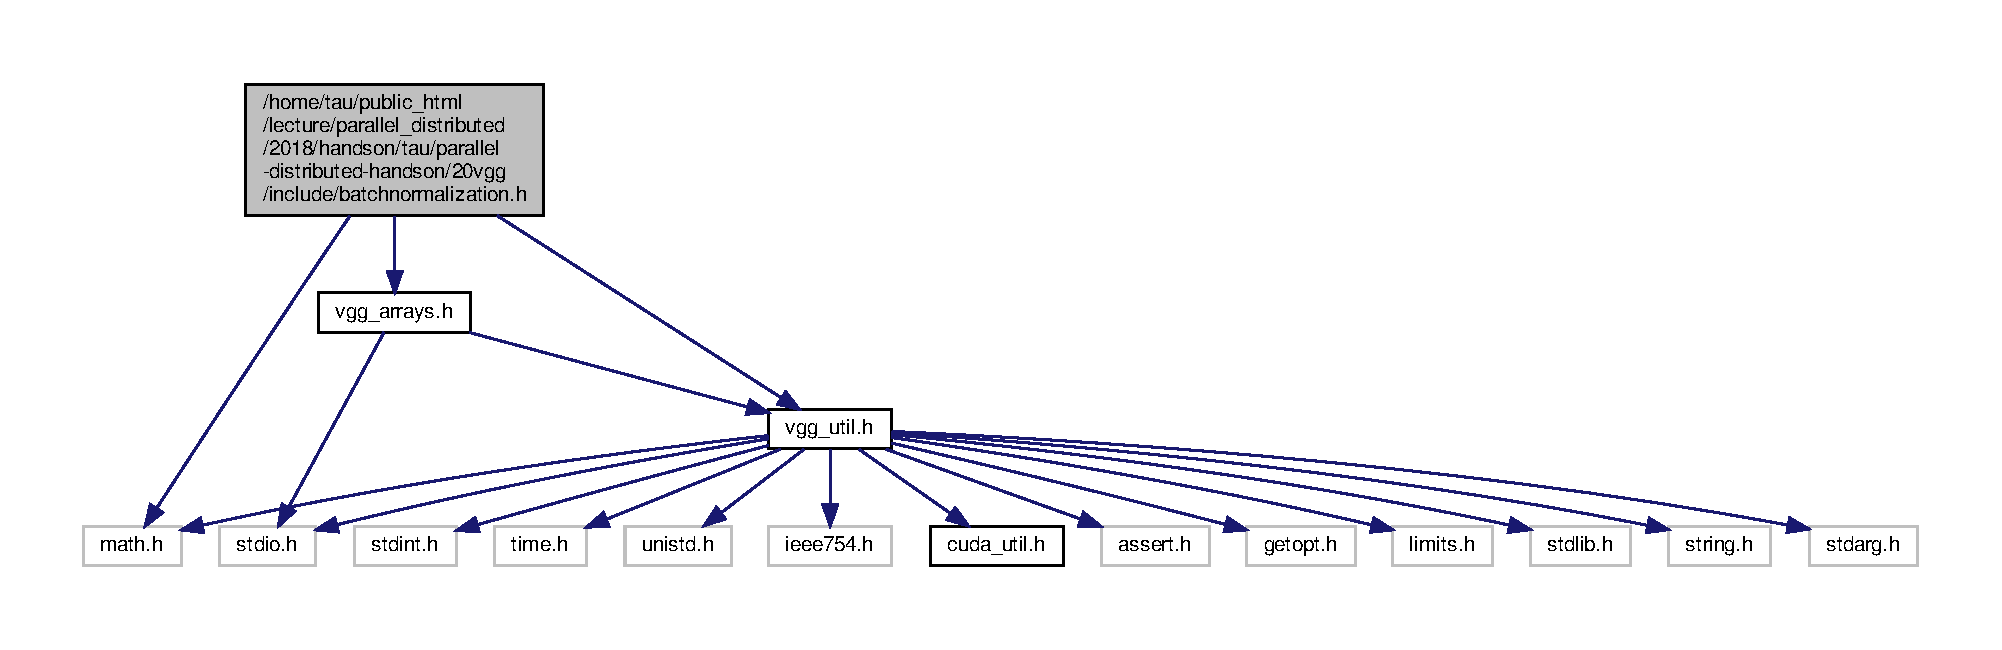
\includegraphics[width=350pt]{batchnormalization_8h__incl}
\end{center}
\end{figure}
This graph shows which files directly or indirectly include this file\+:\nopagebreak
\begin{figure}[H]
\begin{center}
\leavevmode
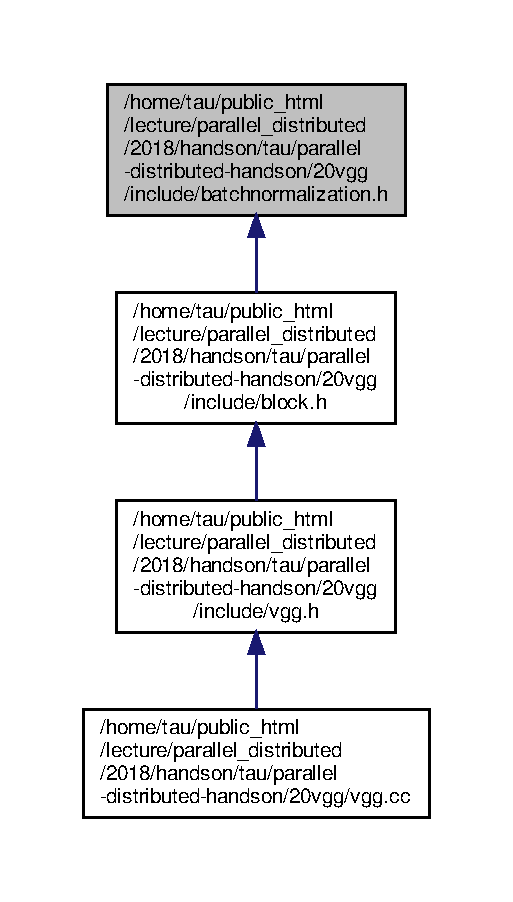
\includegraphics[width=246pt]{batchnormalization_8h__dep__incl}
\end{center}
\end{figure}
\subsection*{Classes}
\begin{DoxyCompactItemize}
\item 
struct \hyperlink{structBatchNormalization}{Batch\+Normalization$<$ max\+B, I\+C, H, W $>$}
\begin{DoxyCompactList}\small\item\em batch normalization \end{DoxyCompactList}\item 
struct \hyperlink{structBatchNormalization}{Batch\+Normalization$<$ max\+B, I\+C, H, W $>$}
\begin{DoxyCompactList}\small\item\em batch normalization \end{DoxyCompactList}\end{DoxyCompactItemize}
\subsection*{Functions}
\begin{DoxyCompactItemize}
\item 
{\footnotesize template$<$idx\+\_\+t maxB, idx\+\_\+t IC, idx\+\_\+t H, idx\+\_\+t W$>$ }\\\+\_\+\+\_\+global\+\_\+\+\_\+ void \hyperlink{batchnormalization_8h_a41bba9077163e208b0b74c48bc543eb1}{forward\+\_\+global} (\hyperlink{structBatchNormalization}{Batch\+Normalization}$<$ maxB, IC, H, W $>$ $\ast$dev, \hyperlink{structarray4}{array4}$<$ maxB, IC, H, W $>$ $\ast$x\+\_\+dev)
\begin{DoxyCompactList}\small\item\em a global C\+U\+DA function that implements the baseline forward function for G\+PU \end{DoxyCompactList}\item 
{\footnotesize template$<$idx\+\_\+t maxB, idx\+\_\+t IC, idx\+\_\+t H, idx\+\_\+t W$>$ }\\\+\_\+\+\_\+global\+\_\+\+\_\+ void \hyperlink{batchnormalization_8h_a1b41e67dca3ea4cfd2f2cc1f60d82ca8}{backward\+\_\+global} (\hyperlink{structBatchNormalization}{Batch\+Normalization}$<$ maxB, IC, H, W $>$ $\ast$dev, \hyperlink{structarray4}{array4}$<$ maxB, IC, H, W $>$ $\ast$gy\+\_\+dev)
\begin{DoxyCompactList}\small\item\em a global C\+U\+DA function that implements the baseline backward function for G\+PU \end{DoxyCompactList}\item 
{\footnotesize template$<$idx\+\_\+t maxB, idx\+\_\+t IC, idx\+\_\+t H, idx\+\_\+t W$>$ }\\\+\_\+\+\_\+global\+\_\+\+\_\+ void \hyperlink{batchnormalization_8h_a50f5ba1511c0f5fdca71aeb753dc7820}{update\+\_\+global} (\hyperlink{structBatchNormalization}{Batch\+Normalization}$<$ maxB, IC, H, W $>$ $\ast$dev, \hyperlink{vgg__util_8h_a1082d08aaa761215ec83e7149f27ad16}{real} eta)
\begin{DoxyCompactList}\small\item\em a global C\+U\+DA function that implements the baseline update function for G\+PU \end{DoxyCompactList}\item 
{\footnotesize template$<$idx\+\_\+t maxB, idx\+\_\+t IC, idx\+\_\+t H, idx\+\_\+t W$>$ }\\static \hyperlink{vgg__util_8h_a1082d08aaa761215ec83e7149f27ad16}{real} \hyperlink{batchnormalization_8h_a06a5c008a0b14db30d206734b44d6f97}{batchnormalization\+\_\+grad\+\_\+check\+\_\+rand} (\hyperlink{structcmdline__opt}{cmdline\+\_\+opt} opt, \hyperlink{structlogger}{logger} $\ast$lgr, \hyperlink{structrnd__gen__t}{rnd\+\_\+gen\+\_\+t} \&rg, \hyperlink{vgg__util_8h_a8e93478a00e685bea5e6a3f617bf03a3}{idx\+\_\+t} B)
\begin{DoxyCompactList}\small\item\em check the gradient computation of a batch normalization layer \end{DoxyCompactList}\item 
int \hyperlink{batchnormalization_8h_af72830784e9693ab42ee8938e518d797}{batchnormalization\+\_\+main} (int argc, char $\ast$$\ast$argv)
\begin{DoxyCompactList}\small\item\em entry point of this header file \end{DoxyCompactList}\end{DoxyCompactItemize}


\subsection{Detailed Description}
batch normalization layer 



\subsection{Function Documentation}
\mbox{\Hypertarget{batchnormalization_8h_a1b41e67dca3ea4cfd2f2cc1f60d82ca8}\label{batchnormalization_8h_a1b41e67dca3ea4cfd2f2cc1f60d82ca8}} 
\index{batchnormalization.\+h@{batchnormalization.\+h}!backward\+\_\+global@{backward\+\_\+global}}
\index{backward\+\_\+global@{backward\+\_\+global}!batchnormalization.\+h@{batchnormalization.\+h}}
\subsubsection{\texorpdfstring{backward\+\_\+global()}{backward\_global()}}
{\footnotesize\ttfamily template$<$idx\+\_\+t maxB, idx\+\_\+t IC, idx\+\_\+t H, idx\+\_\+t W$>$ \\
\+\_\+\+\_\+global\+\_\+\+\_\+ void backward\+\_\+global (\begin{DoxyParamCaption}\item[{\hyperlink{structBatchNormalization}{Batch\+Normalization}$<$ maxB, IC, H, W $>$ $\ast$}]{dev,  }\item[{\hyperlink{structarray4}{array4}$<$ maxB, IC, H, W $>$ $\ast$}]{gy\+\_\+dev }\end{DoxyParamCaption})}



a global C\+U\+DA function that implements the baseline backward function for G\+PU 


\begin{DoxyParams}{Parameters}
{\em (dev)} & the address of the device shadow of the object \\
\hline
{\em (gy\+\_\+dev)} & the address of the device shadow of the input matrix \\
\hline
\end{DoxyParams}
\begin{DoxySeeAlso}{See also}
backward\+\_\+dev 

backward\+\_\+gpu 
\end{DoxySeeAlso}
\mbox{\Hypertarget{batchnormalization_8h_a06a5c008a0b14db30d206734b44d6f97}\label{batchnormalization_8h_a06a5c008a0b14db30d206734b44d6f97}} 
\index{batchnormalization.\+h@{batchnormalization.\+h}!batchnormalization\+\_\+grad\+\_\+check\+\_\+rand@{batchnormalization\+\_\+grad\+\_\+check\+\_\+rand}}
\index{batchnormalization\+\_\+grad\+\_\+check\+\_\+rand@{batchnormalization\+\_\+grad\+\_\+check\+\_\+rand}!batchnormalization.\+h@{batchnormalization.\+h}}
\subsubsection{\texorpdfstring{batchnormalization\+\_\+grad\+\_\+check\+\_\+rand()}{batchnormalization\_grad\_check\_rand()}}
{\footnotesize\ttfamily template$<$idx\+\_\+t maxB, idx\+\_\+t IC, idx\+\_\+t H, idx\+\_\+t W$>$ \\
static \hyperlink{vgg__util_8h_a1082d08aaa761215ec83e7149f27ad16}{real} batchnormalization\+\_\+grad\+\_\+check\+\_\+rand (\begin{DoxyParamCaption}\item[{\hyperlink{structcmdline__opt}{cmdline\+\_\+opt}}]{opt,  }\item[{\hyperlink{structlogger}{logger} $\ast$}]{lgr,  }\item[{\hyperlink{structrnd__gen__t}{rnd\+\_\+gen\+\_\+t} \&}]{rg,  }\item[{\hyperlink{vgg__util_8h_a8e93478a00e685bea5e6a3f617bf03a3}{idx\+\_\+t}}]{B }\end{DoxyParamCaption})\hspace{0.3cm}{\ttfamily [static]}}



check the gradient computation of a batch normalization layer 


\begin{DoxyParams}{Parameters}
{\em (opt)} & command line option \\
\hline
{\em (lgr)} & logger \\
\hline
{\em (rg)} & random number generator \\
\hline
{\em (\+B)} & the number of images \\
\hline
\end{DoxyParams}
\begin{DoxySeeAlso}{See also}
\hyperlink{batchnormalization_8h_af72830784e9693ab42ee8938e518d797}{batchnormalization\+\_\+main}
\end{DoxySeeAlso}
it first makes a layer object with initial weights W and generates an input (x and t). it then creates two layers whose weights are slightly different from the original one by dw/2 (i.\+e., w-\/dw/2 and w+dw/2), as well as two inputs slighly different from the original inputs by dx/2 (x-\/dx/2 and x+dx/2). it then computes L(w,x), L(x-\/dw/2,x-\/dx/2) and L(w+dw/2,x+dw/2) and check if L(x+dw/2,x+dx/2)-\/L(x-\/dw/2,x-\/dx/2) is close to ∂\+L/∂x dx + ∂\+L/∂w dw. ∂\+L/∂x and ∂\+L/∂w are obtained by backward computation. This is essentially checking if the gradients obtained by backward computation correctly approximates the diff of the output. \mbox{\Hypertarget{batchnormalization_8h_af72830784e9693ab42ee8938e518d797}\label{batchnormalization_8h_af72830784e9693ab42ee8938e518d797}} 
\index{batchnormalization.\+h@{batchnormalization.\+h}!batchnormalization\+\_\+main@{batchnormalization\+\_\+main}}
\index{batchnormalization\+\_\+main@{batchnormalization\+\_\+main}!batchnormalization.\+h@{batchnormalization.\+h}}
\subsubsection{\texorpdfstring{batchnormalization\+\_\+main()}{batchnormalization\_main()}}
{\footnotesize\ttfamily int batchnormalization\+\_\+main (\begin{DoxyParamCaption}\item[{int}]{argc,  }\item[{char $\ast$$\ast$}]{argv }\end{DoxyParamCaption})}



entry point of this header file 


\begin{DoxyParams}{Parameters}
{\em (argc)} & the number of command line args \\
\hline
{\em (argv)} & command line args \\
\hline
\end{DoxyParams}
\begin{DoxySeeAlso}{See also}
\hyperlink{batchnormalization_8h_a06a5c008a0b14db30d206734b44d6f97}{batchnormalization\+\_\+grad\+\_\+check\+\_\+rand}
\end{DoxySeeAlso}
if this header file is included from a main C++ file and define batchnormalization\+\_\+main to be main (e.\+g., with -\/\+Dbatchnormalization\+\_\+main=main), then this function becomes th main function of the executable. it calls batchnormalization\+\_\+grad\+\_\+check\+\_\+rand repeatedly to test the implementation of \hyperlink{structVGG}{V\+GG} network. \mbox{\Hypertarget{batchnormalization_8h_a41bba9077163e208b0b74c48bc543eb1}\label{batchnormalization_8h_a41bba9077163e208b0b74c48bc543eb1}} 
\index{batchnormalization.\+h@{batchnormalization.\+h}!forward\+\_\+global@{forward\+\_\+global}}
\index{forward\+\_\+global@{forward\+\_\+global}!batchnormalization.\+h@{batchnormalization.\+h}}
\subsubsection{\texorpdfstring{forward\+\_\+global()}{forward\_global()}}
{\footnotesize\ttfamily template$<$idx\+\_\+t maxB, idx\+\_\+t IC, idx\+\_\+t H, idx\+\_\+t W$>$ \\
\+\_\+\+\_\+global\+\_\+\+\_\+ void forward\+\_\+global (\begin{DoxyParamCaption}\item[{\hyperlink{structBatchNormalization}{Batch\+Normalization}$<$ maxB, IC, H, W $>$ $\ast$}]{dev,  }\item[{\hyperlink{structarray4}{array4}$<$ maxB, IC, H, W $>$ $\ast$}]{x\+\_\+dev }\end{DoxyParamCaption})}



a global C\+U\+DA function that implements the baseline forward function for G\+PU 


\begin{DoxyParams}{Parameters}
{\em (dev)} & the address of the device shadow of the object \\
\hline
{\em (x\+\_\+dev)} & the address of the device shadow of the input matrix \\
\hline
\end{DoxyParams}
\begin{DoxySeeAlso}{See also}
forward\+\_\+dev 

forward\+\_\+gpu 
\end{DoxySeeAlso}
\mbox{\Hypertarget{batchnormalization_8h_a50f5ba1511c0f5fdca71aeb753dc7820}\label{batchnormalization_8h_a50f5ba1511c0f5fdca71aeb753dc7820}} 
\index{batchnormalization.\+h@{batchnormalization.\+h}!update\+\_\+global@{update\+\_\+global}}
\index{update\+\_\+global@{update\+\_\+global}!batchnormalization.\+h@{batchnormalization.\+h}}
\subsubsection{\texorpdfstring{update\+\_\+global()}{update\_global()}}
{\footnotesize\ttfamily template$<$idx\+\_\+t maxB, idx\+\_\+t IC, idx\+\_\+t H, idx\+\_\+t W$>$ \\
\+\_\+\+\_\+global\+\_\+\+\_\+ void update\+\_\+global (\begin{DoxyParamCaption}\item[{\hyperlink{structBatchNormalization}{Batch\+Normalization}$<$ maxB, IC, H, W $>$ $\ast$}]{dev,  }\item[{\hyperlink{vgg__util_8h_a1082d08aaa761215ec83e7149f27ad16}{real}}]{eta }\end{DoxyParamCaption})}



a global C\+U\+DA function that implements the baseline update function for G\+PU 


\begin{DoxyParams}{Parameters}
{\em (dev)} & the address of the device shadow of the object \\
\hline
{\em (eta)} & the address of the device shadow of the input matrix \\
\hline
\end{DoxyParams}
\begin{DoxySeeAlso}{See also}
update\+\_\+dev 

update\+\_\+gpu 
\end{DoxySeeAlso}

\hypertarget{block_8h}{}\section{/home/tau/public\+\_\+html/lecture/parallel\+\_\+distributed/2018/handson/tau/parallel-\/distributed-\/handson/20vgg/include/block.h File Reference}
\label{block_8h}\index{/home/tau/public\+\_\+html/lecture/parallel\+\_\+distributed/2018/handson/tau/parallel-\/distributed-\/handson/20vgg/include/block.\+h@{/home/tau/public\+\_\+html/lecture/parallel\+\_\+distributed/2018/handson/tau/parallel-\/distributed-\/handson/20vgg/include/block.\+h}}


a block of three layers (convolution; batch normalization; relu)  


{\ttfamily \#include \char`\"{}vgg\+\_\+util.\+h\char`\"{}}\newline
{\ttfamily \#include \char`\"{}vgg\+\_\+arrays.\+h\char`\"{}}\newline
{\ttfamily \#include \char`\"{}convolution.\+h\char`\"{}}\newline
{\ttfamily \#include \char`\"{}batchnormalization.\+h\char`\"{}}\newline
{\ttfamily \#include \char`\"{}relu.\+h\char`\"{}}\newline
Include dependency graph for block.\+h\+:
\nopagebreak
\begin{figure}[H]
\begin{center}
\leavevmode
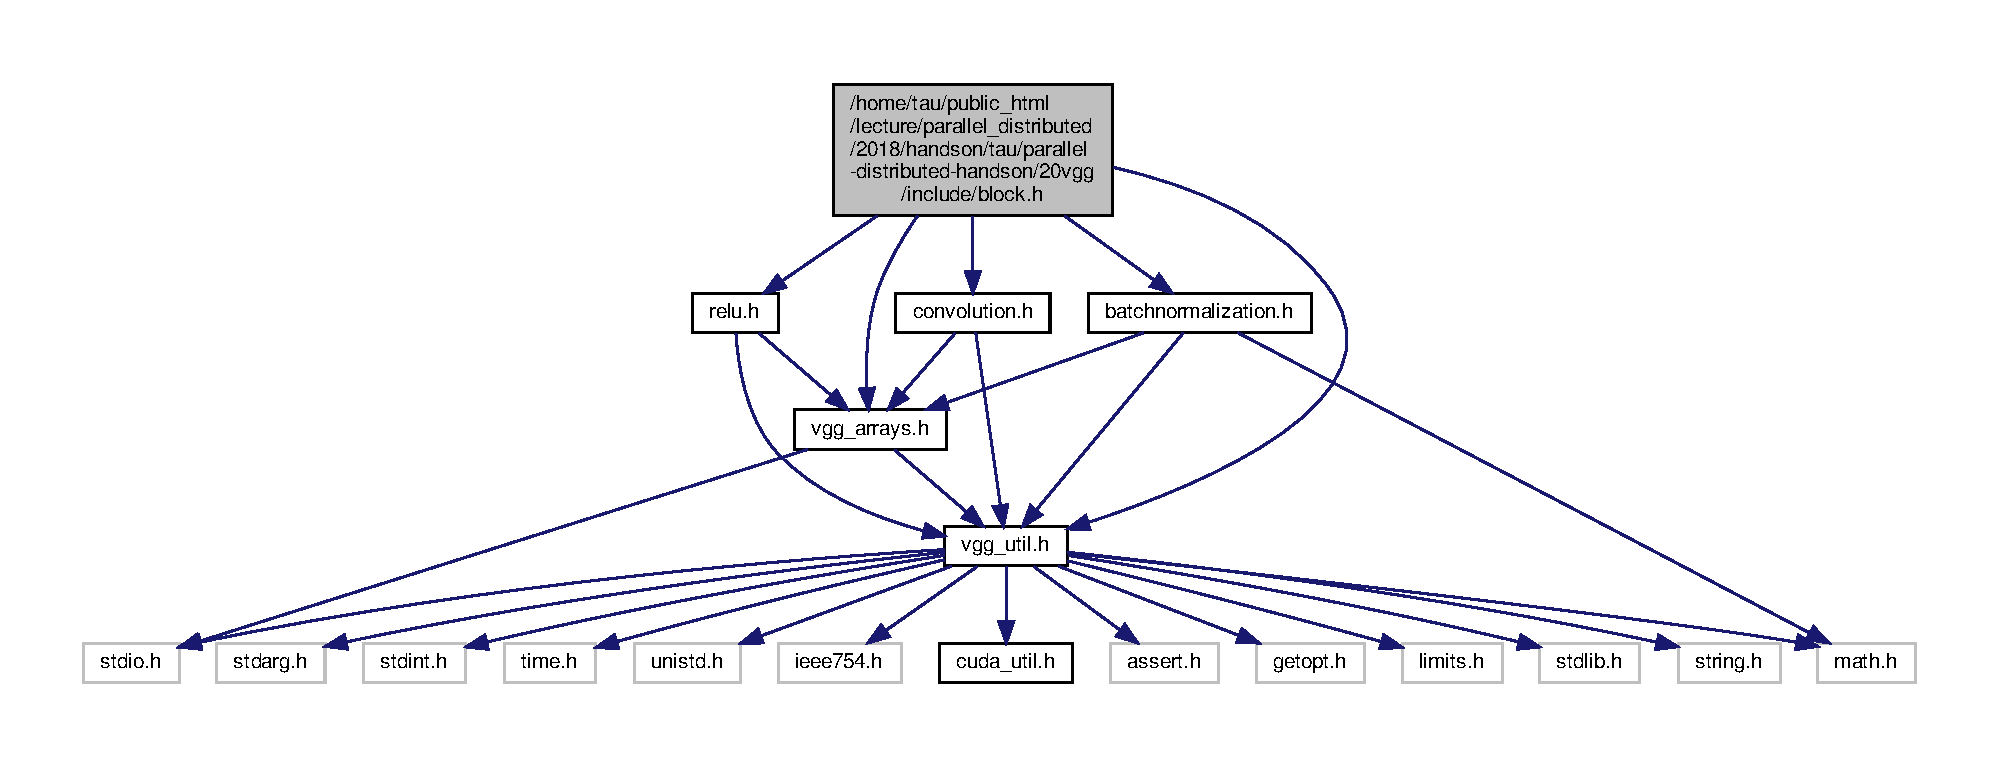
\includegraphics[width=350pt]{block_8h__incl}
\end{center}
\end{figure}
This graph shows which files directly or indirectly include this file\+:
\nopagebreak
\begin{figure}[H]
\begin{center}
\leavevmode
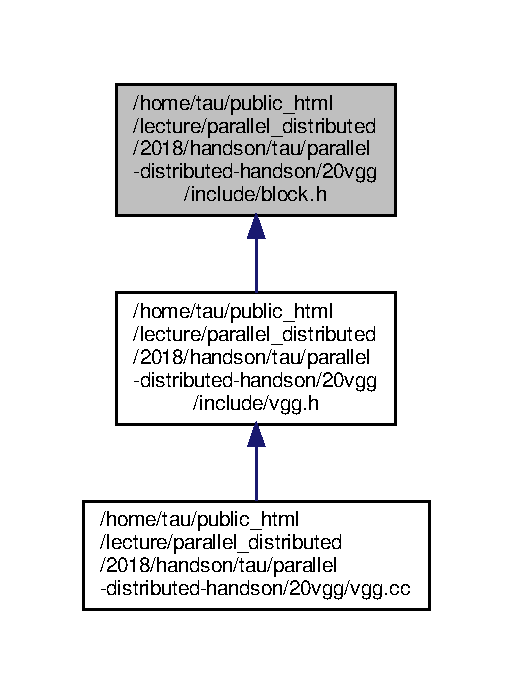
\includegraphics[width=246pt]{block_8h__dep__incl}
\end{center}
\end{figure}
\subsection*{Classes}
\begin{DoxyCompactItemize}
\item 
struct \hyperlink{structBlock}{Block$<$ max\+B, I\+C, H, W, K, O\+C $>$}
\begin{DoxyCompactList}\small\item\em a block of three layers (convolution; batch normalization; relu) \end{DoxyCompactList}\end{DoxyCompactItemize}
\subsection*{Functions}
\begin{DoxyCompactItemize}
\item 
{\footnotesize template$<$idx\+\_\+t maxB, idx\+\_\+t IC, idx\+\_\+t H, idx\+\_\+t W, idx\+\_\+t K, idx\+\_\+t OC$>$ }\\static \hyperlink{vgg__util_8h_a1082d08aaa761215ec83e7149f27ad16}{real} \hyperlink{block_8h_a3aad7f7f1f4137e7c43229f2cf08c166}{block\+\_\+grad\+\_\+check\+\_\+rand} (\hyperlink{structcmdline__opt}{cmdline\+\_\+opt} opt, \hyperlink{structlogger}{logger} $\ast$lgr, \hyperlink{structrnd__gen__t}{rnd\+\_\+gen\+\_\+t} \&rg, \hyperlink{vgg__util_8h_a8e93478a00e685bea5e6a3f617bf03a3}{idx\+\_\+t} B)
\begin{DoxyCompactList}\small\item\em check the gradient computation of a block \end{DoxyCompactList}\item 
int \hyperlink{block_8h_a7a47e99b18d127e5d328a8b917637a8c}{block\+\_\+main} (int argc, char $\ast$$\ast$argv)
\begin{DoxyCompactList}\small\item\em entry point of this header file \end{DoxyCompactList}\end{DoxyCompactItemize}


\subsection{Detailed Description}
a block of three layers (convolution; batch normalization; relu) 



\subsection{Function Documentation}
\mbox{\Hypertarget{block_8h_a3aad7f7f1f4137e7c43229f2cf08c166}\label{block_8h_a3aad7f7f1f4137e7c43229f2cf08c166}} 
\index{block.\+h@{block.\+h}!block\+\_\+grad\+\_\+check\+\_\+rand@{block\+\_\+grad\+\_\+check\+\_\+rand}}
\index{block\+\_\+grad\+\_\+check\+\_\+rand@{block\+\_\+grad\+\_\+check\+\_\+rand}!block.\+h@{block.\+h}}
\subsubsection{\texorpdfstring{block\+\_\+grad\+\_\+check\+\_\+rand()}{block\_grad\_check\_rand()}}
{\footnotesize\ttfamily template$<$idx\+\_\+t maxB, idx\+\_\+t IC, idx\+\_\+t H, idx\+\_\+t W, idx\+\_\+t K, idx\+\_\+t OC$>$ \\
static \hyperlink{vgg__util_8h_a1082d08aaa761215ec83e7149f27ad16}{real} block\+\_\+grad\+\_\+check\+\_\+rand (\begin{DoxyParamCaption}\item[{\hyperlink{structcmdline__opt}{cmdline\+\_\+opt}}]{opt,  }\item[{\hyperlink{structlogger}{logger} $\ast$}]{lgr,  }\item[{\hyperlink{structrnd__gen__t}{rnd\+\_\+gen\+\_\+t} \&}]{rg,  }\item[{\hyperlink{vgg__util_8h_a8e93478a00e685bea5e6a3f617bf03a3}{idx\+\_\+t}}]{B }\end{DoxyParamCaption})\hspace{0.3cm}{\ttfamily [static]}}



check the gradient computation of a block 


\begin{DoxyParams}{Parameters}
{\em (opt)} & command line option \\
\hline
{\em (lgr)} & logger \\
\hline
{\em (rg)} & random number generator \\
\hline
{\em (\+B)} & the number of images \\
\hline
\end{DoxyParams}
\begin{DoxySeeAlso}{See also}
\hyperlink{block_8h_a7a47e99b18d127e5d328a8b917637a8c}{block\+\_\+main}
\end{DoxySeeAlso}
it first makes a block with initial weights W and generates an input (x and t). it then creates two B\+L\+O\+CK networks whose weights are slightly different from the original one by dw/2 (i.\+e., w-\/dw/2 and w+dw/2), as well as two inputs slighly different from the original inputs by dx/2 (x-\/dx/2 and x+dx/2). it then computes L(w,x), L(x-\/dw/2,x-\/dx/2) and L(w+dw/2,x+dw/2) and check if L(x+dw/2,x+dx/2)-\/L(x-\/dw/2,x-\/dx/2) is close to ∂\+L/∂x dx + ∂\+L/∂w dw. ∂\+L/∂x and ∂\+L/∂w are obtained by backward computation. This is essentially checking if the gradients obtained by backward computation correctly approximates the diff of the output. \mbox{\Hypertarget{block_8h_a7a47e99b18d127e5d328a8b917637a8c}\label{block_8h_a7a47e99b18d127e5d328a8b917637a8c}} 
\index{block.\+h@{block.\+h}!block\+\_\+main@{block\+\_\+main}}
\index{block\+\_\+main@{block\+\_\+main}!block.\+h@{block.\+h}}
\subsubsection{\texorpdfstring{block\+\_\+main()}{block\_main()}}
{\footnotesize\ttfamily int block\+\_\+main (\begin{DoxyParamCaption}\item[{int}]{argc,  }\item[{char $\ast$$\ast$}]{argv }\end{DoxyParamCaption})}



entry point of this header file 


\begin{DoxyParams}{Parameters}
{\em (argc)} & the number of command line args \\
\hline
{\em (argv)} & command line args \\
\hline
\end{DoxyParams}
\begin{DoxySeeAlso}{See also}
\hyperlink{block_8h_a3aad7f7f1f4137e7c43229f2cf08c166}{block\+\_\+grad\+\_\+check\+\_\+rand}
\end{DoxySeeAlso}
if this header file is included from a main C++ file and define block\+\_\+main to be main (e.\+g., with -\/\+Dblock\+\_\+main=main), then this function becomes th main function of the executable. it calls block\+\_\+grad\+\_\+check\+\_\+rand repeatedly to test the implementation of block. 
\hypertarget{cifar_8h}{}\section{/home/tau/public\+\_\+html/lecture/parallel\+\_\+distributed/2018/handson/tau/parallel-\/distributed-\/handson/20vgg/include/cifar.h File Reference}
\label{cifar_8h}\index{/home/tau/public\+\_\+html/lecture/parallel\+\_\+distributed/2018/handson/tau/parallel-\/distributed-\/handson/20vgg/include/cifar.\+h@{/home/tau/public\+\_\+html/lecture/parallel\+\_\+distributed/2018/handson/tau/parallel-\/distributed-\/handson/20vgg/include/cifar.\+h}}


cifar dataset handling  


{\ttfamily \#include $<$sys/types.\+h$>$}\newline
{\ttfamily \#include $<$sys/stat.\+h$>$}\newline
{\ttfamily \#include $<$unistd.\+h$>$}\newline
{\ttfamily \#include \char`\"{}vgg\+\_\+util.\+h\char`\"{}}\newline
{\ttfamily \#include \char`\"{}vgg\+\_\+arrays.\+h\char`\"{}}\newline
Include dependency graph for cifar.\+h\+:\nopagebreak
\begin{figure}[H]
\begin{center}
\leavevmode
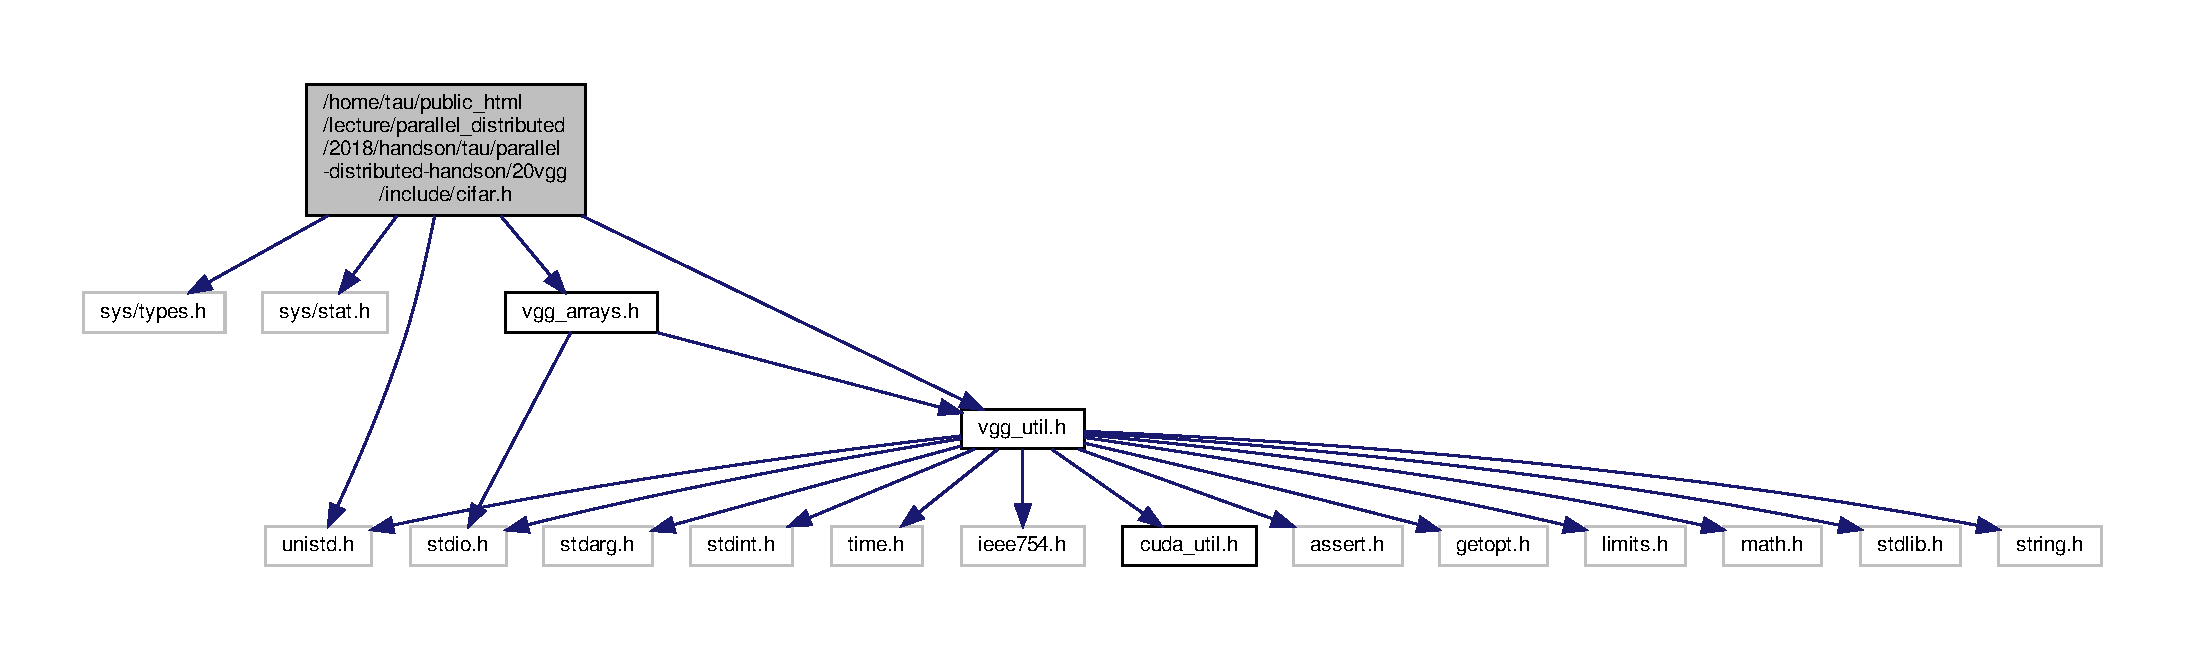
\includegraphics[width=350pt]{cifar_8h__incl}
\end{center}
\end{figure}
This graph shows which files directly or indirectly include this file\+:\nopagebreak
\begin{figure}[H]
\begin{center}
\leavevmode
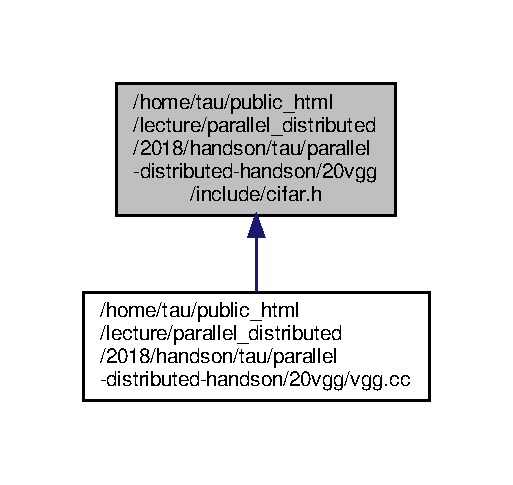
\includegraphics[width=246pt]{cifar_8h__dep__incl}
\end{center}
\end{figure}
\subsection*{Classes}
\begin{DoxyCompactItemize}
\item 
struct \hyperlink{structcifar10__data__item}{cifar10\+\_\+data\+\_\+item$<$ I\+C, H, W $>$}
\begin{DoxyCompactList}\small\item\em an input + true label \end{DoxyCompactList}\item 
struct \hyperlink{structcifar10__dataset}{cifar10\+\_\+dataset$<$ max\+B, I\+C, H, W $>$}
\begin{DoxyCompactList}\small\item\em an entire cifar10 data \end{DoxyCompactList}\end{DoxyCompactItemize}
\subsection*{Functions}
\begin{DoxyCompactItemize}
\item 
int \hyperlink{cifar_8h_a65bc263a51effffc5e5c83e475bee9a2}{cifar\+\_\+main} (int argc, char $\ast$$\ast$argv)
\begin{DoxyCompactList}\small\item\em entry point of this header file \end{DoxyCompactList}\end{DoxyCompactItemize}


\subsection{Detailed Description}
cifar dataset handling 



\subsection{Function Documentation}
\mbox{\Hypertarget{cifar_8h_a65bc263a51effffc5e5c83e475bee9a2}\label{cifar_8h_a65bc263a51effffc5e5c83e475bee9a2}} 
\index{cifar.\+h@{cifar.\+h}!cifar\+\_\+main@{cifar\+\_\+main}}
\index{cifar\+\_\+main@{cifar\+\_\+main}!cifar.\+h@{cifar.\+h}}
\subsubsection{\texorpdfstring{cifar\+\_\+main()}{cifar\_main()}}
{\footnotesize\ttfamily int cifar\+\_\+main (\begin{DoxyParamCaption}\item[{int}]{argc,  }\item[{char $\ast$$\ast$}]{argv }\end{DoxyParamCaption})}



entry point of this header file 


\begin{DoxyParams}{Parameters}
{\em (argc)} & the number of command line args \\
\hline
{\em (argv)} & command line args \\
\hline
\end{DoxyParams}

\hypertarget{convolution_8h}{}\section{/home/tau/public\+\_\+html/lecture/parallel\+\_\+distributed/2018/handson/tau/parallel-\/distributed-\/handson/20vgg/include/convolution.h File Reference}
\label{convolution_8h}\index{/home/tau/public\+\_\+html/lecture/parallel\+\_\+distributed/2018/handson/tau/parallel-\/distributed-\/handson/20vgg/include/convolution.\+h@{/home/tau/public\+\_\+html/lecture/parallel\+\_\+distributed/2018/handson/tau/parallel-\/distributed-\/handson/20vgg/include/convolution.\+h}}


convolution layer  


{\ttfamily \#include \char`\"{}vgg\+\_\+util.\+h\char`\"{}}\newline
{\ttfamily \#include \char`\"{}vgg\+\_\+arrays.\+h\char`\"{}}\newline
Include dependency graph for convolution.\+h\+:\nopagebreak
\begin{figure}[H]
\begin{center}
\leavevmode
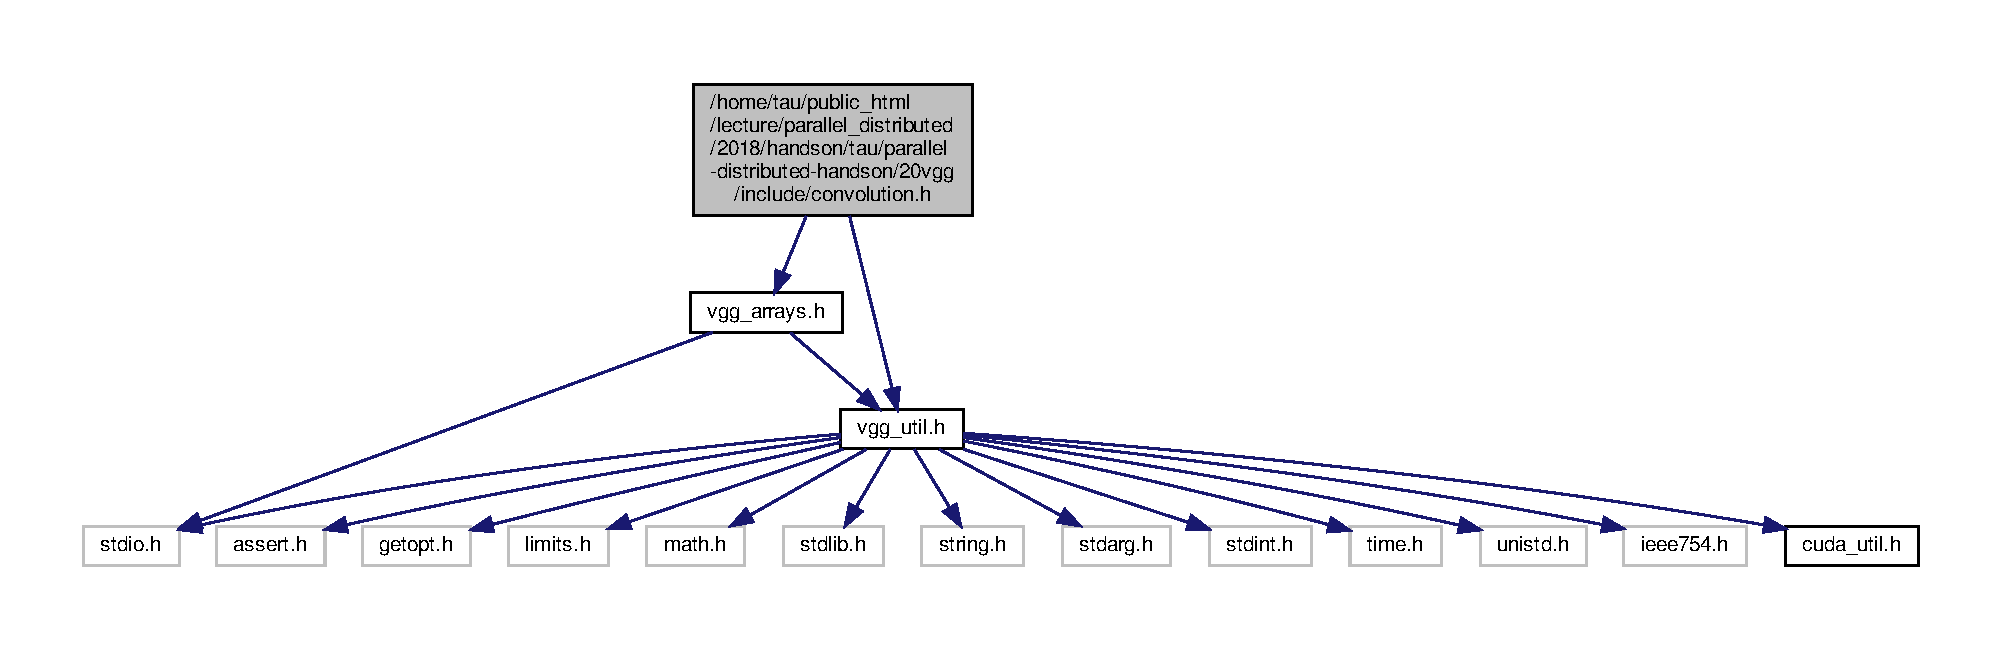
\includegraphics[width=350pt]{convolution_8h__incl}
\end{center}
\end{figure}
This graph shows which files directly or indirectly include this file\+:\nopagebreak
\begin{figure}[H]
\begin{center}
\leavevmode
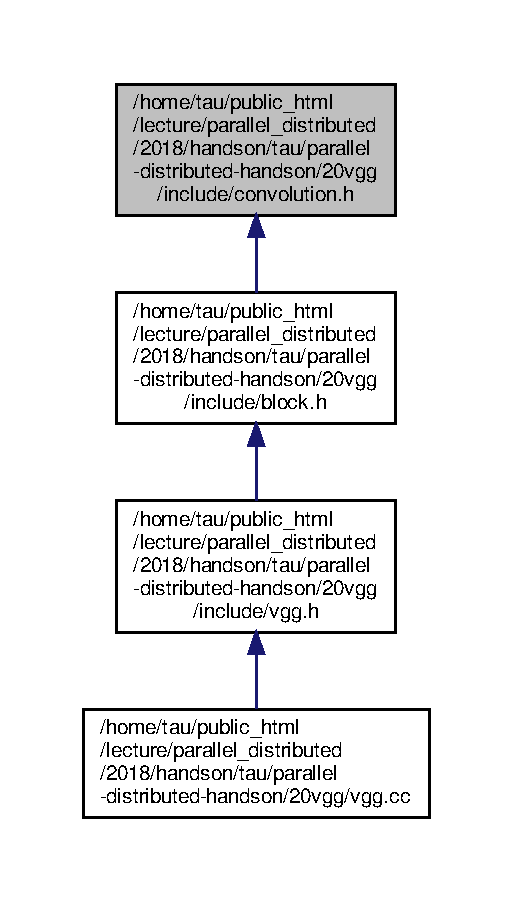
\includegraphics[width=246pt]{convolution_8h__dep__incl}
\end{center}
\end{figure}
\subsection*{Classes}
\begin{DoxyCompactItemize}
\item 
struct \hyperlink{structConvolution2D}{Convolution2\+D$<$ max\+B, I\+C, H, W, K, O\+C $>$}
\begin{DoxyCompactList}\small\item\em convolution of images \end{DoxyCompactList}\item 
struct \hyperlink{structConvolution2D}{Convolution2\+D$<$ max\+B, I\+C, H, W, K, O\+C $>$}
\begin{DoxyCompactList}\small\item\em convolution of images \end{DoxyCompactList}\end{DoxyCompactItemize}
\subsection*{Functions}
\begin{DoxyCompactItemize}
\item 
{\footnotesize template$<$idx\+\_\+t maxB, idx\+\_\+t IC, idx\+\_\+t H, idx\+\_\+t W, idx\+\_\+t K, idx\+\_\+t OC$>$ }\\\+\_\+\+\_\+global\+\_\+\+\_\+ void \hyperlink{convolution_8h_a66f12281fd34d13e31a607f799beff87}{forward\+\_\+global} (\hyperlink{structConvolution2D}{Convolution2D}$<$ maxB, IC, H, W, K, OC $>$ $\ast$dev, \hyperlink{structarray4}{array4}$<$ maxB, IC, H, W $>$ $\ast$x\+\_\+dev)
\begin{DoxyCompactList}\small\item\em a global C\+U\+DA function that implements the baseline forward function for G\+PU \end{DoxyCompactList}\item 
{\footnotesize template$<$idx\+\_\+t maxB, idx\+\_\+t IC, idx\+\_\+t H, idx\+\_\+t W, idx\+\_\+t K, idx\+\_\+t OC$>$ }\\\+\_\+\+\_\+global\+\_\+\+\_\+ void \hyperlink{convolution_8h_a932da028868c7cd27665143fa27353cc}{backward\+\_\+global} (\hyperlink{structConvolution2D}{Convolution2D}$<$ maxB, IC, H, W, K, OC $>$ $\ast$dev, \hyperlink{structarray4}{array4}$<$ maxB, OC, H, W $>$ $\ast$gy\+\_\+dev)
\begin{DoxyCompactList}\small\item\em a global C\+U\+DA function that implements the baseline backward function for G\+PU \end{DoxyCompactList}\item 
{\footnotesize template$<$idx\+\_\+t maxB, idx\+\_\+t IC, idx\+\_\+t H, idx\+\_\+t W, idx\+\_\+t K, idx\+\_\+t OC$>$ }\\\+\_\+\+\_\+global\+\_\+\+\_\+ void \hyperlink{convolution_8h_a983bc98cc731aa417ca07a3067b45a8e}{update\+\_\+global} (\hyperlink{structConvolution2D}{Convolution2D}$<$ maxB, IC, H, W, K, OC $>$ $\ast$dev, \hyperlink{vgg__util_8h_a1082d08aaa761215ec83e7149f27ad16}{real} eta)
\begin{DoxyCompactList}\small\item\em a global C\+U\+DA function that implements the baseline update function for G\+PU \end{DoxyCompactList}\item 
{\footnotesize template$<$idx\+\_\+t maxB, idx\+\_\+t IC, idx\+\_\+t H, idx\+\_\+t W, idx\+\_\+t K, idx\+\_\+t OC$>$ }\\static \hyperlink{vgg__util_8h_a1082d08aaa761215ec83e7149f27ad16}{real} \hyperlink{convolution_8h_a9430c272fe1b8403588552cbccfd465c}{convolution\+\_\+grad\+\_\+check\+\_\+rand} (\hyperlink{structcmdline__opt}{cmdline\+\_\+opt} opt, \hyperlink{structlogger}{logger} $\ast$lgr, \hyperlink{structrnd__gen__t}{rnd\+\_\+gen\+\_\+t} \&rg, \hyperlink{vgg__util_8h_a8e93478a00e685bea5e6a3f617bf03a3}{idx\+\_\+t} B)
\begin{DoxyCompactList}\small\item\em check the gradient computation of a convolution layer \end{DoxyCompactList}\item 
int \hyperlink{convolution_8h_a023046a04d2db321418e3f6f6a917bde}{convolution\+\_\+main} (int argc, char $\ast$$\ast$argv)
\begin{DoxyCompactList}\small\item\em entry point of this header file \end{DoxyCompactList}\end{DoxyCompactItemize}


\subsection{Detailed Description}
convolution layer 



\subsection{Function Documentation}
\mbox{\Hypertarget{convolution_8h_a932da028868c7cd27665143fa27353cc}\label{convolution_8h_a932da028868c7cd27665143fa27353cc}} 
\index{convolution.\+h@{convolution.\+h}!backward\+\_\+global@{backward\+\_\+global}}
\index{backward\+\_\+global@{backward\+\_\+global}!convolution.\+h@{convolution.\+h}}
\subsubsection{\texorpdfstring{backward\+\_\+global()}{backward\_global()}}
{\footnotesize\ttfamily template$<$idx\+\_\+t maxB, idx\+\_\+t IC, idx\+\_\+t H, idx\+\_\+t W, idx\+\_\+t K, idx\+\_\+t OC$>$ \\
\+\_\+\+\_\+global\+\_\+\+\_\+ void backward\+\_\+global (\begin{DoxyParamCaption}\item[{\hyperlink{structConvolution2D}{Convolution2D}$<$ maxB, IC, H, W, K, OC $>$ $\ast$}]{dev,  }\item[{\hyperlink{structarray4}{array4}$<$ maxB, OC, H, W $>$ $\ast$}]{gy\+\_\+dev }\end{DoxyParamCaption})}



a global C\+U\+DA function that implements the baseline backward function for G\+PU 


\begin{DoxyParams}{Parameters}
{\em (dev)} & the address of the device shadow of the object \\
\hline
{\em (gy\+\_\+dev)} & the address of the device shadow of the input matrix \\
\hline
\end{DoxyParams}
\begin{DoxySeeAlso}{See also}
backward\+\_\+dev 

backward\+\_\+gpu 
\end{DoxySeeAlso}
\mbox{\Hypertarget{convolution_8h_a9430c272fe1b8403588552cbccfd465c}\label{convolution_8h_a9430c272fe1b8403588552cbccfd465c}} 
\index{convolution.\+h@{convolution.\+h}!convolution\+\_\+grad\+\_\+check\+\_\+rand@{convolution\+\_\+grad\+\_\+check\+\_\+rand}}
\index{convolution\+\_\+grad\+\_\+check\+\_\+rand@{convolution\+\_\+grad\+\_\+check\+\_\+rand}!convolution.\+h@{convolution.\+h}}
\subsubsection{\texorpdfstring{convolution\+\_\+grad\+\_\+check\+\_\+rand()}{convolution\_grad\_check\_rand()}}
{\footnotesize\ttfamily template$<$idx\+\_\+t maxB, idx\+\_\+t IC, idx\+\_\+t H, idx\+\_\+t W, idx\+\_\+t K, idx\+\_\+t OC$>$ \\
static \hyperlink{vgg__util_8h_a1082d08aaa761215ec83e7149f27ad16}{real} convolution\+\_\+grad\+\_\+check\+\_\+rand (\begin{DoxyParamCaption}\item[{\hyperlink{structcmdline__opt}{cmdline\+\_\+opt}}]{opt,  }\item[{\hyperlink{structlogger}{logger} $\ast$}]{lgr,  }\item[{\hyperlink{structrnd__gen__t}{rnd\+\_\+gen\+\_\+t} \&}]{rg,  }\item[{\hyperlink{vgg__util_8h_a8e93478a00e685bea5e6a3f617bf03a3}{idx\+\_\+t}}]{B }\end{DoxyParamCaption})\hspace{0.3cm}{\ttfamily [static]}}



check the gradient computation of a convolution layer 


\begin{DoxyParams}{Parameters}
{\em (opt)} & command line option \\
\hline
{\em (lgr)} & logger \\
\hline
{\em (rg)} & random number generator \\
\hline
{\em (\+B)} & the number of images \\
\hline
\end{DoxyParams}
\begin{DoxySeeAlso}{See also}
\hyperlink{convolution_8h_a023046a04d2db321418e3f6f6a917bde}{convolution\+\_\+main}
\end{DoxySeeAlso}
it first makes a layer object with initial weights W and generates an input (x and t). it then creates two layers whose weights are slightly different from the original one by dw/2 (i.\+e., w-\/dw/2 and w+dw/2), as well as two inputs slighly different from the original inputs by dx/2 (x-\/dx/2 and x+dx/2). it then computes L(w,x), L(x-\/dw/2,x-\/dx/2) and L(w+dw/2,x+dw/2) and check if L(x+dw/2,x+dx/2)-\/L(x-\/dw/2,x-\/dx/2) is close to ∂\+L/∂x dx + ∂\+L/∂w dw. ∂\+L/∂x and ∂\+L/∂w are obtained by backward computation. This is essentially checking if the gradients obtained by backward computation correctly approximates the diff of the output. \mbox{\Hypertarget{convolution_8h_a023046a04d2db321418e3f6f6a917bde}\label{convolution_8h_a023046a04d2db321418e3f6f6a917bde}} 
\index{convolution.\+h@{convolution.\+h}!convolution\+\_\+main@{convolution\+\_\+main}}
\index{convolution\+\_\+main@{convolution\+\_\+main}!convolution.\+h@{convolution.\+h}}
\subsubsection{\texorpdfstring{convolution\+\_\+main()}{convolution\_main()}}
{\footnotesize\ttfamily int convolution\+\_\+main (\begin{DoxyParamCaption}\item[{int}]{argc,  }\item[{char $\ast$$\ast$}]{argv }\end{DoxyParamCaption})}



entry point of this header file 


\begin{DoxyParams}{Parameters}
{\em (argc)} & the number of command line args \\
\hline
{\em (argv)} & command line args \\
\hline
\end{DoxyParams}
\begin{DoxySeeAlso}{See also}
\hyperlink{convolution_8h_a9430c272fe1b8403588552cbccfd465c}{convolution\+\_\+grad\+\_\+check\+\_\+rand}
\end{DoxySeeAlso}
if this header file is included from a main C++ file and define convolution\+\_\+main to be main (e.\+g., with -\/\+Dconvolution\+\_\+main=main), then this function becomes th main function of the executable. it calls convolution\+\_\+grad\+\_\+check\+\_\+rand repeatedly to test the implementation of \hyperlink{structVGG}{V\+GG} network. \mbox{\Hypertarget{convolution_8h_a66f12281fd34d13e31a607f799beff87}\label{convolution_8h_a66f12281fd34d13e31a607f799beff87}} 
\index{convolution.\+h@{convolution.\+h}!forward\+\_\+global@{forward\+\_\+global}}
\index{forward\+\_\+global@{forward\+\_\+global}!convolution.\+h@{convolution.\+h}}
\subsubsection{\texorpdfstring{forward\+\_\+global()}{forward\_global()}}
{\footnotesize\ttfamily template$<$idx\+\_\+t maxB, idx\+\_\+t IC, idx\+\_\+t H, idx\+\_\+t W, idx\+\_\+t K, idx\+\_\+t OC$>$ \\
\+\_\+\+\_\+global\+\_\+\+\_\+ void forward\+\_\+global (\begin{DoxyParamCaption}\item[{\hyperlink{structConvolution2D}{Convolution2D}$<$ maxB, IC, H, W, K, OC $>$ $\ast$}]{dev,  }\item[{\hyperlink{structarray4}{array4}$<$ maxB, IC, H, W $>$ $\ast$}]{x\+\_\+dev }\end{DoxyParamCaption})}



a global C\+U\+DA function that implements the baseline forward function for G\+PU 


\begin{DoxyParams}{Parameters}
{\em (dev)} & the address of the device shadow of the object \\
\hline
{\em (x\+\_\+dev)} & the address of the device shadow of the input matrix \\
\hline
\end{DoxyParams}
\begin{DoxySeeAlso}{See also}
forward\+\_\+dev 

forward\+\_\+gpu 
\end{DoxySeeAlso}
\mbox{\Hypertarget{convolution_8h_a983bc98cc731aa417ca07a3067b45a8e}\label{convolution_8h_a983bc98cc731aa417ca07a3067b45a8e}} 
\index{convolution.\+h@{convolution.\+h}!update\+\_\+global@{update\+\_\+global}}
\index{update\+\_\+global@{update\+\_\+global}!convolution.\+h@{convolution.\+h}}
\subsubsection{\texorpdfstring{update\+\_\+global()}{update\_global()}}
{\footnotesize\ttfamily template$<$idx\+\_\+t maxB, idx\+\_\+t IC, idx\+\_\+t H, idx\+\_\+t W, idx\+\_\+t K, idx\+\_\+t OC$>$ \\
\+\_\+\+\_\+global\+\_\+\+\_\+ void update\+\_\+global (\begin{DoxyParamCaption}\item[{\hyperlink{structConvolution2D}{Convolution2D}$<$ maxB, IC, H, W, K, OC $>$ $\ast$}]{dev,  }\item[{\hyperlink{vgg__util_8h_a1082d08aaa761215ec83e7149f27ad16}{real}}]{eta }\end{DoxyParamCaption})}



a global C\+U\+DA function that implements the baseline update function for G\+PU 


\begin{DoxyParams}{Parameters}
{\em (dev)} & the address of the device shadow of the object \\
\hline
{\em (eta)} & the address of the device shadow of the input matrix \\
\hline
\end{DoxyParams}
\begin{DoxySeeAlso}{See also}
update\+\_\+dev 

update\+\_\+gpu 
\end{DoxySeeAlso}

\hypertarget{cuda__util_8h}{}\section{/home/tau/public\+\_\+html/lecture/parallel\+\_\+distributed/2018/handson/tau/parallel-\/distributed-\/handson/20vgg/include/cuda\+\_\+util.h File Reference}
\label{cuda__util_8h}\index{/home/tau/public\+\_\+html/lecture/parallel\+\_\+distributed/2018/handson/tau/parallel-\/distributed-\/handson/20vgg/include/cuda\+\_\+util.\+h@{/home/tau/public\+\_\+html/lecture/parallel\+\_\+distributed/2018/handson/tau/parallel-\/distributed-\/handson/20vgg/include/cuda\+\_\+util.\+h}}


small utility functions for cuda  


This graph shows which files directly or indirectly include this file\+:\nopagebreak
\begin{figure}[H]
\begin{center}
\leavevmode
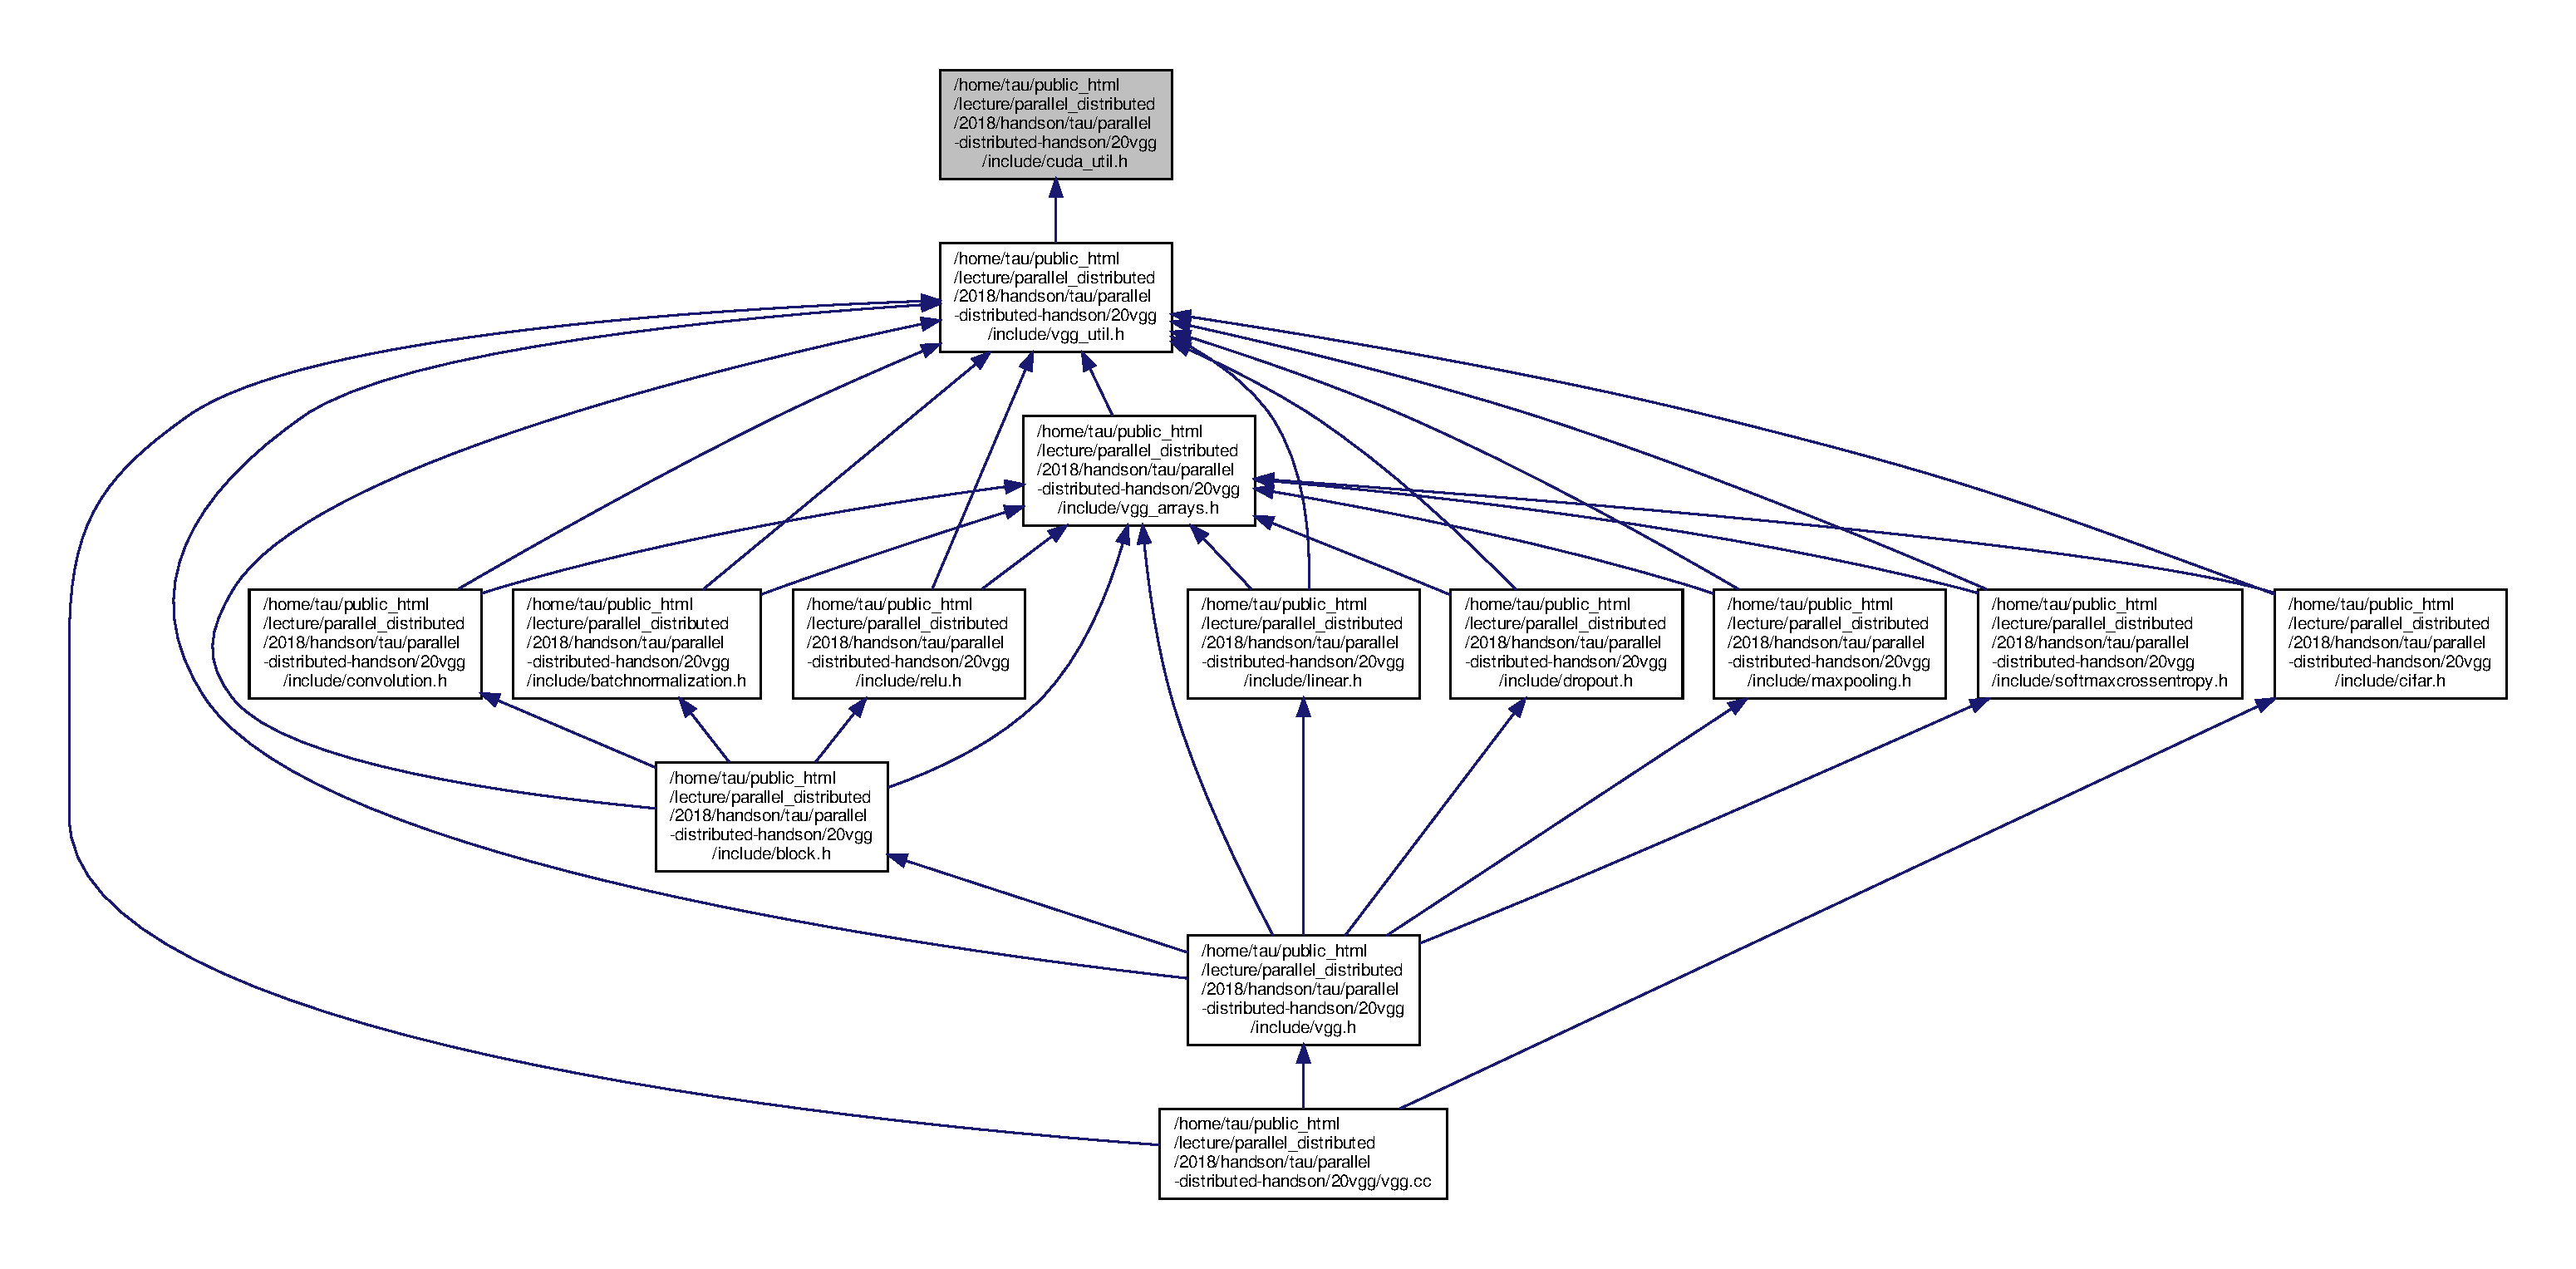
\includegraphics[width=350pt]{cuda__util_8h__dep__incl}
\end{center}
\end{figure}
\subsection*{Macros}
\begin{DoxyCompactItemize}
\item 
\#define \hyperlink{cuda__util_8h_ae08da20e750e9eabdf37c5cdf87a6e73}{check\+\_\+api\+\_\+error}(e)~\hyperlink{cuda__util_8h_afe8e81182b6d9bdc912e4477ea7f6221}{check\+\_\+api\+\_\+error\+\_\+}(e, \#e, \+\_\+\+\_\+\+F\+I\+L\+E\+\_\+\+\_\+, \+\_\+\+\_\+\+L\+I\+N\+E\+\_\+\+\_\+)
\begin{DoxyCompactList}\small\item\em check if a C\+U\+DA A\+PI invocation succeeded and show the error msg if any \end{DoxyCompactList}\item 
\#define \hyperlink{cuda__util_8h_ae8a9e1ffcd7af83a818bc9a6ec7bed78}{check\+\_\+launch\+\_\+error}(exp)~do \{ exp; \hyperlink{cuda__util_8h_a522422f538aba091ae7b9ec113871075}{check\+\_\+launch\+\_\+error\+\_\+}(\#exp, \+\_\+\+\_\+\+F\+I\+L\+E\+\_\+\+\_\+, \+\_\+\+\_\+\+L\+I\+N\+E\+\_\+\+\_\+); \} while (0)
\begin{DoxyCompactList}\small\item\em check kernel launch error \end{DoxyCompactList}\item 
\#define \hyperlink{cuda__util_8h_ae7d73cb485e300b743d0cb70eaa38f31}{launch\+\_\+and\+\_\+sync}(exp)~do \{ exp; \hyperlink{cuda__util_8h_a522422f538aba091ae7b9ec113871075}{check\+\_\+launch\+\_\+error\+\_\+}(\#exp, \+\_\+\+\_\+\+F\+I\+L\+E\+\_\+\+\_\+, \+\_\+\+\_\+\+L\+I\+N\+E\+\_\+\+\_\+); \hyperlink{cuda__util_8h_abeb2ea962924754e9f3009cd444e0d7c}{dev\+\_\+sync}(); \} while (0)
\begin{DoxyCompactList}\small\item\em launch a kernel and wait for its completion \end{DoxyCompactList}\end{DoxyCompactItemize}
\subsection*{Functions}
\begin{DoxyCompactItemize}
\item 
static void \hyperlink{cuda__util_8h_afe8e81182b6d9bdc912e4477ea7f6221}{check\+\_\+api\+\_\+error\+\_\+} (cuda\+Error\+\_\+t e, const char $\ast$msg, const char $\ast$file, int line)
\begin{DoxyCompactList}\small\item\em do not use this function directly. use check\+\_\+api\+\_\+error macro \end{DoxyCompactList}\item 
static void \hyperlink{cuda__util_8h_a522422f538aba091ae7b9ec113871075}{check\+\_\+launch\+\_\+error\+\_\+} (const char $\ast$msg, const char $\ast$file, int line)
\begin{DoxyCompactList}\small\item\em do not use this function directly. use check\+\_\+launch\+\_\+error macro \end{DoxyCompactList}\item 
\mbox{\Hypertarget{cuda__util_8h_abeb2ea962924754e9f3009cd444e0d7c}\label{cuda__util_8h_abeb2ea962924754e9f3009cd444e0d7c}} 
static void \hyperlink{cuda__util_8h_abeb2ea962924754e9f3009cd444e0d7c}{dev\+\_\+sync} ()
\begin{DoxyCompactList}\small\item\em wrap cuda\+Device\+Synchronize with error check \end{DoxyCompactList}\item 
\mbox{\Hypertarget{cuda__util_8h_a42ba739c08e201d58f7a031d899a0e7f}\label{cuda__util_8h_a42ba739c08e201d58f7a031d899a0e7f}} 
\+\_\+\+\_\+device\+\_\+\+\_\+ uint \hyperlink{cuda__util_8h_a42ba739c08e201d58f7a031d899a0e7f}{get\+\_\+smid} (void)
\begin{DoxyCompactList}\small\item\em get SM executing the caller \end{DoxyCompactList}\item 
\mbox{\Hypertarget{cuda__util_8h_a859de24e23ee0450818ab96ea6a4798a}\label{cuda__util_8h_a859de24e23ee0450818ab96ea6a4798a}} 
static int \hyperlink{cuda__util_8h_a859de24e23ee0450818ab96ea6a4798a}{get\+\_\+freq} ()
\begin{DoxyCompactList}\small\item\em get device frequency \end{DoxyCompactList}\item 
\mbox{\Hypertarget{cuda__util_8h_afefb7dee05552efd8d1e91a09c90dc79}\label{cuda__util_8h_afefb7dee05552efd8d1e91a09c90dc79}} 
static void $\ast$ \hyperlink{cuda__util_8h_afefb7dee05552efd8d1e91a09c90dc79}{dev\+\_\+malloc} (size\+\_\+t sz)
\begin{DoxyCompactList}\small\item\em wrap cuda\+Malloc. cuda\+Malloc + error check + more ordinary malloc-\/like interface (return pointer) \end{DoxyCompactList}\item 
\mbox{\Hypertarget{cuda__util_8h_ade14b7c582717d436e547ed0fcf8e4fe}\label{cuda__util_8h_ade14b7c582717d436e547ed0fcf8e4fe}} 
static void \hyperlink{cuda__util_8h_ade14b7c582717d436e547ed0fcf8e4fe}{dev\+\_\+free} (void $\ast$a)
\begin{DoxyCompactList}\small\item\em wrap cuda\+Free \end{DoxyCompactList}\item 
\mbox{\Hypertarget{cuda__util_8h_a0737678a7fc54cb0347e3c4178ad5dfa}\label{cuda__util_8h_a0737678a7fc54cb0347e3c4178ad5dfa}} 
void \hyperlink{cuda__util_8h_a0737678a7fc54cb0347e3c4178ad5dfa}{to\+\_\+host} (void $\ast$dst, void $\ast$src, size\+\_\+t sz)
\begin{DoxyCompactList}\small\item\em wrap cuda\+Memcpy to copy from device to host (and check an error if any) \end{DoxyCompactList}\item 
\mbox{\Hypertarget{cuda__util_8h_a7b851642eafb77c5d1945bcf81916d7c}\label{cuda__util_8h_a7b851642eafb77c5d1945bcf81916d7c}} 
static void \hyperlink{cuda__util_8h_a7b851642eafb77c5d1945bcf81916d7c}{to\+\_\+dev} (void $\ast$dst, void $\ast$src, size\+\_\+t sz)
\begin{DoxyCompactList}\small\item\em wrap cuda\+Memcpy to copy from host to device (and check an error if any) \end{DoxyCompactList}\item 
\mbox{\Hypertarget{cuda__util_8h_a30655f0f077528b999634c85513af4b0}\label{cuda__util_8h_a30655f0f077528b999634c85513af4b0}} 
\+\_\+\+\_\+device\+\_\+\+\_\+ int \hyperlink{cuda__util_8h_a30655f0f077528b999634c85513af4b0}{get\+\_\+thread\+\_\+id\+\_\+x} ()
\begin{DoxyCompactList}\small\item\em thread ID along x-\/dimension \end{DoxyCompactList}\item 
\mbox{\Hypertarget{cuda__util_8h_a6ea184310bf6fc2e1313127215aab5b0}\label{cuda__util_8h_a6ea184310bf6fc2e1313127215aab5b0}} 
\+\_\+\+\_\+device\+\_\+\+\_\+ int \hyperlink{cuda__util_8h_a6ea184310bf6fc2e1313127215aab5b0}{get\+\_\+thread\+\_\+id\+\_\+y} ()
\begin{DoxyCompactList}\small\item\em thread ID along y-\/dimension \end{DoxyCompactList}\item 
\mbox{\Hypertarget{cuda__util_8h_afff8c5c6d0e85b4a264786a4170ad777}\label{cuda__util_8h_afff8c5c6d0e85b4a264786a4170ad777}} 
\+\_\+\+\_\+device\+\_\+\+\_\+ int \hyperlink{cuda__util_8h_afff8c5c6d0e85b4a264786a4170ad777}{get\+\_\+thread\+\_\+id\+\_\+z} ()
\begin{DoxyCompactList}\small\item\em thread ID along z-\/dimension \end{DoxyCompactList}\item 
\mbox{\Hypertarget{cuda__util_8h_ae13980c33ac8f950ed35d613415034c0}\label{cuda__util_8h_ae13980c33ac8f950ed35d613415034c0}} 
\+\_\+\+\_\+device\+\_\+\+\_\+ int \hyperlink{cuda__util_8h_ae13980c33ac8f950ed35d613415034c0}{get\+\_\+nthreads\+\_\+x} ()
\begin{DoxyCompactList}\small\item\em number of threads along x-\/dimension \end{DoxyCompactList}\item 
\mbox{\Hypertarget{cuda__util_8h_a79fd9ff68db3a81b8b0feb446e4e9b99}\label{cuda__util_8h_a79fd9ff68db3a81b8b0feb446e4e9b99}} 
\+\_\+\+\_\+device\+\_\+\+\_\+ int \hyperlink{cuda__util_8h_a79fd9ff68db3a81b8b0feb446e4e9b99}{get\+\_\+nthreads\+\_\+y} ()
\begin{DoxyCompactList}\small\item\em number of threads along y-\/dimension \end{DoxyCompactList}\item 
\mbox{\Hypertarget{cuda__util_8h_a59cd23ec9bc1ab07e3eaac1ad3e109b4}\label{cuda__util_8h_a59cd23ec9bc1ab07e3eaac1ad3e109b4}} 
\+\_\+\+\_\+device\+\_\+\+\_\+ int \hyperlink{cuda__util_8h_a59cd23ec9bc1ab07e3eaac1ad3e109b4}{get\+\_\+nthreads\+\_\+z} ()
\begin{DoxyCompactList}\small\item\em number of threads along z-\/dimension \end{DoxyCompactList}\item 
\mbox{\Hypertarget{cuda__util_8h_ace44c6e6794929ce9e48e1122c7a3a12}\label{cuda__util_8h_ace44c6e6794929ce9e48e1122c7a3a12}} 
\+\_\+\+\_\+device\+\_\+\+\_\+ int \hyperlink{cuda__util_8h_ace44c6e6794929ce9e48e1122c7a3a12}{get\+\_\+thread\+\_\+id} ()
\begin{DoxyCompactList}\small\item\em global (x,y,z combined into an integer) thread ID \end{DoxyCompactList}\item 
\mbox{\Hypertarget{cuda__util_8h_a74d008c0d996e10f203bdd1fdee76511}\label{cuda__util_8h_a74d008c0d996e10f203bdd1fdee76511}} 
\+\_\+\+\_\+device\+\_\+\+\_\+ int \hyperlink{cuda__util_8h_a74d008c0d996e10f203bdd1fdee76511}{get\+\_\+nthreads} ()
\begin{DoxyCompactList}\small\item\em total number of threads \end{DoxyCompactList}\end{DoxyCompactItemize}


\subsection{Detailed Description}
small utility functions for cuda 

\begin{DoxyAuthor}{Author}
Kenjiro Taura 
\end{DoxyAuthor}
\begin{DoxyDate}{Date}
Oct. 14, 2018 
\end{DoxyDate}


\subsection{Macro Definition Documentation}
\mbox{\Hypertarget{cuda__util_8h_ae08da20e750e9eabdf37c5cdf87a6e73}\label{cuda__util_8h_ae08da20e750e9eabdf37c5cdf87a6e73}} 
\index{cuda\+\_\+util.\+h@{cuda\+\_\+util.\+h}!check\+\_\+api\+\_\+error@{check\+\_\+api\+\_\+error}}
\index{check\+\_\+api\+\_\+error@{check\+\_\+api\+\_\+error}!cuda\+\_\+util.\+h@{cuda\+\_\+util.\+h}}
\subsubsection{\texorpdfstring{check\+\_\+api\+\_\+error}{check\_api\_error}}
{\footnotesize\ttfamily \#define check\+\_\+api\+\_\+error(\begin{DoxyParamCaption}\item[{}]{e }\end{DoxyParamCaption})~\hyperlink{cuda__util_8h_afe8e81182b6d9bdc912e4477ea7f6221}{check\+\_\+api\+\_\+error\+\_\+}(e, \#e, \+\_\+\+\_\+\+F\+I\+L\+E\+\_\+\+\_\+, \+\_\+\+\_\+\+L\+I\+N\+E\+\_\+\+\_\+)}



check if a C\+U\+DA A\+PI invocation succeeded and show the error msg if any 

usage\+: \hyperlink{cuda__util_8h_ae08da20e750e9eabdf37c5cdf87a6e73}{check\+\_\+api\+\_\+error(cuda\+\_\+api\+\_\+call())}. for example, \hyperlink{cuda__util_8h_ae08da20e750e9eabdf37c5cdf87a6e73}{check\+\_\+api\+\_\+error(cuda\+Malloc(\&p, size))}; \mbox{\Hypertarget{cuda__util_8h_ae8a9e1ffcd7af83a818bc9a6ec7bed78}\label{cuda__util_8h_ae8a9e1ffcd7af83a818bc9a6ec7bed78}} 
\index{cuda\+\_\+util.\+h@{cuda\+\_\+util.\+h}!check\+\_\+launch\+\_\+error@{check\+\_\+launch\+\_\+error}}
\index{check\+\_\+launch\+\_\+error@{check\+\_\+launch\+\_\+error}!cuda\+\_\+util.\+h@{cuda\+\_\+util.\+h}}
\subsubsection{\texorpdfstring{check\+\_\+launch\+\_\+error}{check\_launch\_error}}
{\footnotesize\ttfamily \#define check\+\_\+launch\+\_\+error(\begin{DoxyParamCaption}\item[{}]{exp }\end{DoxyParamCaption})~do \{ exp; \hyperlink{cuda__util_8h_a522422f538aba091ae7b9ec113871075}{check\+\_\+launch\+\_\+error\+\_\+}(\#exp, \+\_\+\+\_\+\+F\+I\+L\+E\+\_\+\+\_\+, \+\_\+\+\_\+\+L\+I\+N\+E\+\_\+\+\_\+); \} while (0)}



check kernel launch error 

usage\+: check\+\_\+launch\+\_\+error((kernel-\/launch-\/expression)). for example, check\+\_\+launch\+\_\+error((your\+\_\+gpu\+\_\+kernel$<$$<$$<$n\+\_\+blocks,block\+\_\+sz$>$$>$$>$(a,b,c))). note that you need to put parens around the expression. \mbox{\Hypertarget{cuda__util_8h_ae7d73cb485e300b743d0cb70eaa38f31}\label{cuda__util_8h_ae7d73cb485e300b743d0cb70eaa38f31}} 
\index{cuda\+\_\+util.\+h@{cuda\+\_\+util.\+h}!launch\+\_\+and\+\_\+sync@{launch\+\_\+and\+\_\+sync}}
\index{launch\+\_\+and\+\_\+sync@{launch\+\_\+and\+\_\+sync}!cuda\+\_\+util.\+h@{cuda\+\_\+util.\+h}}
\subsubsection{\texorpdfstring{launch\+\_\+and\+\_\+sync}{launch\_and\_sync}}
{\footnotesize\ttfamily \#define launch\+\_\+and\+\_\+sync(\begin{DoxyParamCaption}\item[{}]{exp }\end{DoxyParamCaption})~do \{ exp; \hyperlink{cuda__util_8h_a522422f538aba091ae7b9ec113871075}{check\+\_\+launch\+\_\+error\+\_\+}(\#exp, \+\_\+\+\_\+\+F\+I\+L\+E\+\_\+\+\_\+, \+\_\+\+\_\+\+L\+I\+N\+E\+\_\+\+\_\+); \hyperlink{cuda__util_8h_abeb2ea962924754e9f3009cd444e0d7c}{dev\+\_\+sync}(); \} while (0)}



launch a kernel and wait for its completion 

usage\+: launch\+\_\+and\+\_\+sync((kernel-\/launch-\/expression)). for example, launch\+\_\+and\+\_\+sync((your\+\_\+gpu\+\_\+kernel$<$$<$$<$n\+\_\+blocks,block\+\_\+sz$>$$>$$>$(a,b,c))). note that you need to put parens around the expression. 

\subsection{Function Documentation}
\mbox{\Hypertarget{cuda__util_8h_afe8e81182b6d9bdc912e4477ea7f6221}\label{cuda__util_8h_afe8e81182b6d9bdc912e4477ea7f6221}} 
\index{cuda\+\_\+util.\+h@{cuda\+\_\+util.\+h}!check\+\_\+api\+\_\+error\+\_\+@{check\+\_\+api\+\_\+error\+\_\+}}
\index{check\+\_\+api\+\_\+error\+\_\+@{check\+\_\+api\+\_\+error\+\_\+}!cuda\+\_\+util.\+h@{cuda\+\_\+util.\+h}}
\subsubsection{\texorpdfstring{check\+\_\+api\+\_\+error\+\_\+()}{check\_api\_error\_()}}
{\footnotesize\ttfamily static void check\+\_\+api\+\_\+error\+\_\+ (\begin{DoxyParamCaption}\item[{cuda\+Error\+\_\+t}]{e,  }\item[{const char $\ast$}]{msg,  }\item[{const char $\ast$}]{file,  }\item[{int}]{line }\end{DoxyParamCaption})\hspace{0.3cm}{\ttfamily [static]}}



do not use this function directly. use check\+\_\+api\+\_\+error macro 

\begin{DoxySeeAlso}{See also}
\hyperlink{cuda__util_8h_ae08da20e750e9eabdf37c5cdf87a6e73}{check\+\_\+api\+\_\+error} 
\end{DoxySeeAlso}
\mbox{\Hypertarget{cuda__util_8h_a522422f538aba091ae7b9ec113871075}\label{cuda__util_8h_a522422f538aba091ae7b9ec113871075}} 
\index{cuda\+\_\+util.\+h@{cuda\+\_\+util.\+h}!check\+\_\+launch\+\_\+error\+\_\+@{check\+\_\+launch\+\_\+error\+\_\+}}
\index{check\+\_\+launch\+\_\+error\+\_\+@{check\+\_\+launch\+\_\+error\+\_\+}!cuda\+\_\+util.\+h@{cuda\+\_\+util.\+h}}
\subsubsection{\texorpdfstring{check\+\_\+launch\+\_\+error\+\_\+()}{check\_launch\_error\_()}}
{\footnotesize\ttfamily static void check\+\_\+launch\+\_\+error\+\_\+ (\begin{DoxyParamCaption}\item[{const char $\ast$}]{msg,  }\item[{const char $\ast$}]{file,  }\item[{int}]{line }\end{DoxyParamCaption})\hspace{0.3cm}{\ttfamily [static]}}



do not use this function directly. use check\+\_\+launch\+\_\+error macro 

\begin{DoxySeeAlso}{See also}
\hyperlink{cuda__util_8h_ae8a9e1ffcd7af83a818bc9a6ec7bed78}{check\+\_\+launch\+\_\+error} 
\end{DoxySeeAlso}

\hypertarget{dropout_8h}{}\section{/home/tau/public\+\_\+html/lecture/parallel\+\_\+distributed/2018/handson/tau/parallel-\/distributed-\/handson/20vgg/include/dropout.h File Reference}
\label{dropout_8h}\index{/home/tau/public\+\_\+html/lecture/parallel\+\_\+distributed/2018/handson/tau/parallel-\/distributed-\/handson/20vgg/include/dropout.\+h@{/home/tau/public\+\_\+html/lecture/parallel\+\_\+distributed/2018/handson/tau/parallel-\/distributed-\/handson/20vgg/include/dropout.\+h}}


dropout layer  


{\ttfamily \#include \char`\"{}vgg\+\_\+util.\+h\char`\"{}}\newline
{\ttfamily \#include \char`\"{}vgg\+\_\+arrays.\+h\char`\"{}}\newline
Include dependency graph for dropout.\+h\+:\nopagebreak
\begin{figure}[H]
\begin{center}
\leavevmode
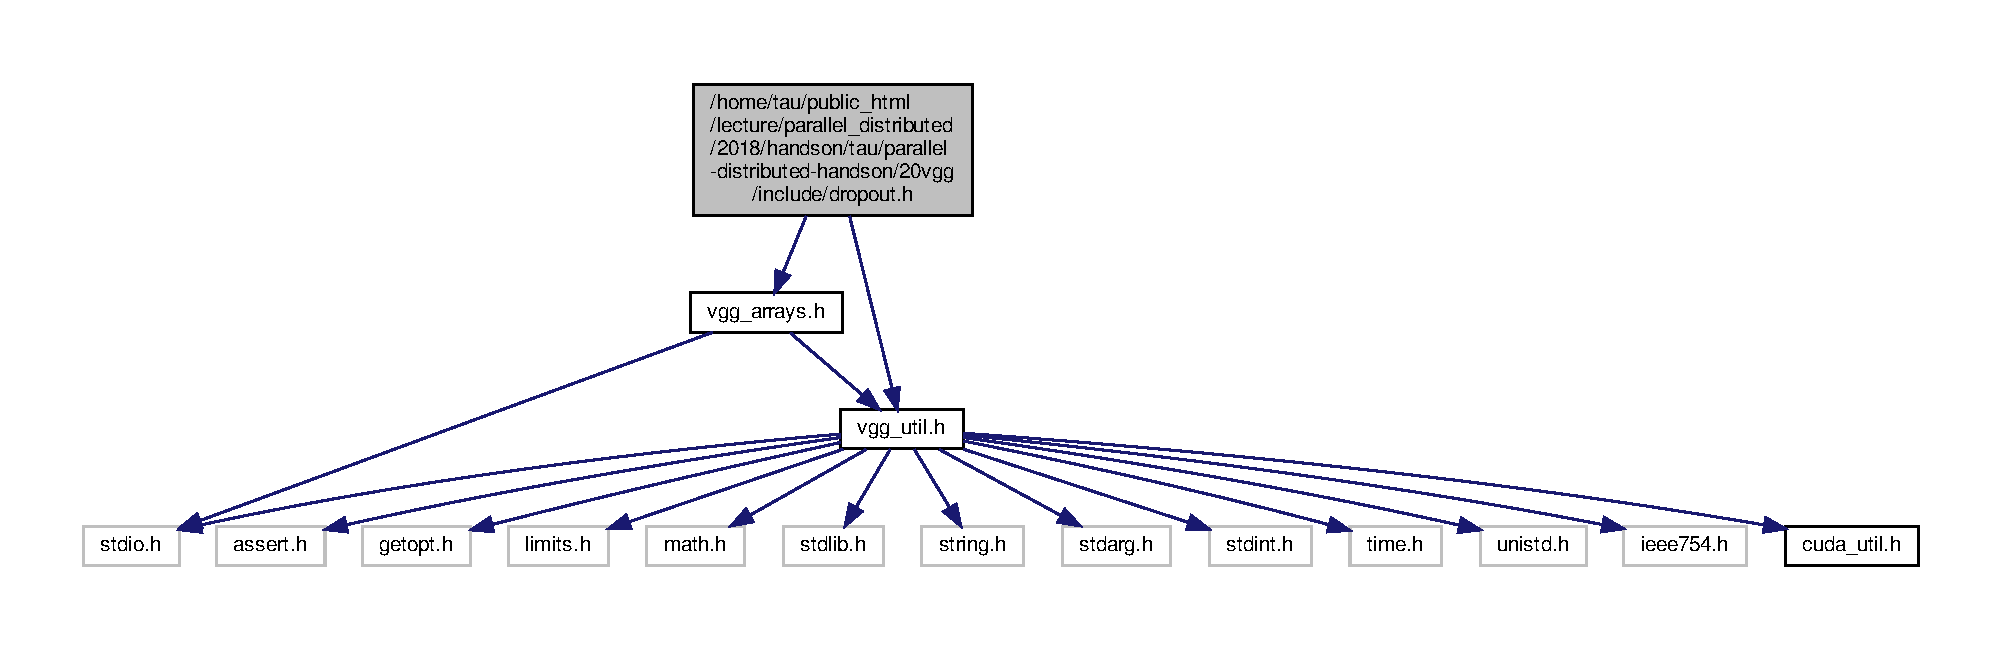
\includegraphics[width=350pt]{dropout_8h__incl}
\end{center}
\end{figure}
This graph shows which files directly or indirectly include this file\+:\nopagebreak
\begin{figure}[H]
\begin{center}
\leavevmode
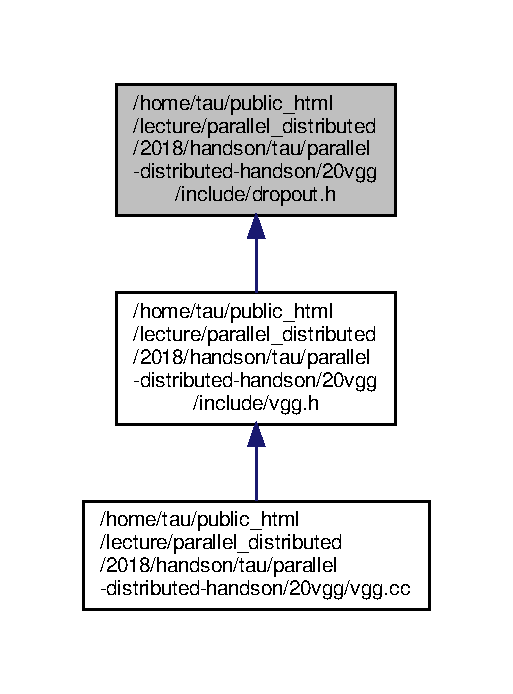
\includegraphics[width=246pt]{dropout_8h__dep__incl}
\end{center}
\end{figure}
\subsection*{Classes}
\begin{DoxyCompactItemize}
\item 
struct \hyperlink{structDropout}{Dropout$<$ max\+B, C, H, W $>$}
\begin{DoxyCompactList}\small\item\em dropout layer \end{DoxyCompactList}\item 
struct \hyperlink{structDropout}{Dropout$<$ max\+B, C, H, W $>$}
\begin{DoxyCompactList}\small\item\em dropout layer \end{DoxyCompactList}\end{DoxyCompactItemize}
\subsection*{Functions}
\begin{DoxyCompactItemize}
\item 
{\footnotesize template$<$idx\+\_\+t maxB, idx\+\_\+t C, idx\+\_\+t H, idx\+\_\+t W$>$ }\\\+\_\+\+\_\+global\+\_\+\+\_\+ void \hyperlink{dropout_8h_a481b6aac35e6819a36e87b00866a2cf8}{forward\+\_\+global} (\hyperlink{structDropout}{Dropout}$<$ maxB, C, H, W $>$ $\ast$dev, \hyperlink{structarray4}{array4}$<$ maxB, C, H, W $>$ $\ast$x\+\_\+dev)
\begin{DoxyCompactList}\small\item\em a global C\+U\+DA function that implements the baseline forward function for G\+PU \end{DoxyCompactList}\item 
{\footnotesize template$<$idx\+\_\+t maxB, idx\+\_\+t C, idx\+\_\+t H, idx\+\_\+t W$>$ }\\\+\_\+\+\_\+global\+\_\+\+\_\+ void \hyperlink{dropout_8h_a1eba1ae8b54b7b1ac7da64793993f58a}{backward\+\_\+global} (\hyperlink{structDropout}{Dropout}$<$ maxB, C, H, W $>$ $\ast$dev, \hyperlink{structarray4}{array4}$<$ maxB, C, H, W $>$ $\ast$gy\+\_\+dev)
\begin{DoxyCompactList}\small\item\em a global C\+U\+DA function that implements the baseline backward function for G\+PU \end{DoxyCompactList}\item 
{\footnotesize template$<$idx\+\_\+t maxB, idx\+\_\+t C, idx\+\_\+t H, idx\+\_\+t W$>$ }\\static \hyperlink{vgg__util_8h_a1082d08aaa761215ec83e7149f27ad16}{real} \hyperlink{dropout_8h_a3078a106aefd1416b053dfc6aa2cef8f}{dropout\+\_\+grad\+\_\+check\+\_\+rand} (\hyperlink{structcmdline__opt}{cmdline\+\_\+opt} opt, \hyperlink{structlogger}{logger} $\ast$lgr, \hyperlink{structrnd__gen__t}{rnd\+\_\+gen\+\_\+t} \&rg, \hyperlink{vgg__util_8h_a8e93478a00e685bea5e6a3f617bf03a3}{idx\+\_\+t} B)
\begin{DoxyCompactList}\small\item\em check the gradient computation of a dropout layer \end{DoxyCompactList}\item 
int \hyperlink{dropout_8h_a4ef5b975a86f550ff6e75094a34a88bf}{dropout\+\_\+main} (int argc, char $\ast$$\ast$argv)
\begin{DoxyCompactList}\small\item\em entry point of this header file \end{DoxyCompactList}\end{DoxyCompactItemize}


\subsection{Detailed Description}
dropout layer 



\subsection{Function Documentation}
\mbox{\Hypertarget{dropout_8h_a1eba1ae8b54b7b1ac7da64793993f58a}\label{dropout_8h_a1eba1ae8b54b7b1ac7da64793993f58a}} 
\index{dropout.\+h@{dropout.\+h}!backward\+\_\+global@{backward\+\_\+global}}
\index{backward\+\_\+global@{backward\+\_\+global}!dropout.\+h@{dropout.\+h}}
\subsubsection{\texorpdfstring{backward\+\_\+global()}{backward\_global()}}
{\footnotesize\ttfamily template$<$idx\+\_\+t maxB, idx\+\_\+t C, idx\+\_\+t H, idx\+\_\+t W$>$ \\
\+\_\+\+\_\+global\+\_\+\+\_\+ void backward\+\_\+global (\begin{DoxyParamCaption}\item[{\hyperlink{structDropout}{Dropout}$<$ maxB, C, H, W $>$ $\ast$}]{dev,  }\item[{\hyperlink{structarray4}{array4}$<$ maxB, C, H, W $>$ $\ast$}]{gy\+\_\+dev }\end{DoxyParamCaption})}



a global C\+U\+DA function that implements the baseline backward function for G\+PU 


\begin{DoxyParams}{Parameters}
{\em (dev)} & the address of the device shadow of the object \\
\hline
{\em (gy\+\_\+dev)} & the address of the device shadow of the input matrix \\
\hline
\end{DoxyParams}
\begin{DoxySeeAlso}{See also}
backward\+\_\+dev 

backward\+\_\+gpu 
\end{DoxySeeAlso}
\mbox{\Hypertarget{dropout_8h_a3078a106aefd1416b053dfc6aa2cef8f}\label{dropout_8h_a3078a106aefd1416b053dfc6aa2cef8f}} 
\index{dropout.\+h@{dropout.\+h}!dropout\+\_\+grad\+\_\+check\+\_\+rand@{dropout\+\_\+grad\+\_\+check\+\_\+rand}}
\index{dropout\+\_\+grad\+\_\+check\+\_\+rand@{dropout\+\_\+grad\+\_\+check\+\_\+rand}!dropout.\+h@{dropout.\+h}}
\subsubsection{\texorpdfstring{dropout\+\_\+grad\+\_\+check\+\_\+rand()}{dropout\_grad\_check\_rand()}}
{\footnotesize\ttfamily template$<$idx\+\_\+t maxB, idx\+\_\+t C, idx\+\_\+t H, idx\+\_\+t W$>$ \\
static \hyperlink{vgg__util_8h_a1082d08aaa761215ec83e7149f27ad16}{real} dropout\+\_\+grad\+\_\+check\+\_\+rand (\begin{DoxyParamCaption}\item[{\hyperlink{structcmdline__opt}{cmdline\+\_\+opt}}]{opt,  }\item[{\hyperlink{structlogger}{logger} $\ast$}]{lgr,  }\item[{\hyperlink{structrnd__gen__t}{rnd\+\_\+gen\+\_\+t} \&}]{rg,  }\item[{\hyperlink{vgg__util_8h_a8e93478a00e685bea5e6a3f617bf03a3}{idx\+\_\+t}}]{B }\end{DoxyParamCaption})\hspace{0.3cm}{\ttfamily [static]}}



check the gradient computation of a dropout layer 


\begin{DoxyParams}{Parameters}
{\em (opt)} & command line option \\
\hline
{\em (lgr)} & logger \\
\hline
{\em (rg)} & random number generator \\
\hline
{\em (\+B)} & the number of images \\
\hline
\end{DoxyParams}
\begin{DoxySeeAlso}{See also}
\hyperlink{dropout_8h_a4ef5b975a86f550ff6e75094a34a88bf}{dropout\+\_\+main}
\end{DoxySeeAlso}
it first makes a layer object with initial weights W and generates an input (x and t). it then creates two layers whose weights are slightly different from the original one by dw/2 (i.\+e., w-\/dw/2 and w+dw/2), as well as two inputs slighly different from the original inputs by dx/2 (x-\/dx/2 and x+dx/2). it then computes L(w,x), L(x-\/dw/2,x-\/dx/2) and L(w+dw/2,x+dw/2) and check if L(x+dw/2,x+dx/2)-\/L(x-\/dw/2,x-\/dx/2) is close to ∂\+L/∂x dx + ∂\+L/∂w dw. ∂\+L/∂x and ∂\+L/∂w are obtained by backward computation. This is essentially checking if the gradients obtained by backward computation correctly approximates the diff of the output. \mbox{\Hypertarget{dropout_8h_a4ef5b975a86f550ff6e75094a34a88bf}\label{dropout_8h_a4ef5b975a86f550ff6e75094a34a88bf}} 
\index{dropout.\+h@{dropout.\+h}!dropout\+\_\+main@{dropout\+\_\+main}}
\index{dropout\+\_\+main@{dropout\+\_\+main}!dropout.\+h@{dropout.\+h}}
\subsubsection{\texorpdfstring{dropout\+\_\+main()}{dropout\_main()}}
{\footnotesize\ttfamily int dropout\+\_\+main (\begin{DoxyParamCaption}\item[{int}]{argc,  }\item[{char $\ast$$\ast$}]{argv }\end{DoxyParamCaption})}



entry point of this header file 


\begin{DoxyParams}{Parameters}
{\em (argc)} & the number of command line args \\
\hline
{\em (argv)} & command line args \\
\hline
\end{DoxyParams}
\begin{DoxySeeAlso}{See also}
\hyperlink{dropout_8h_a3078a106aefd1416b053dfc6aa2cef8f}{dropout\+\_\+grad\+\_\+check\+\_\+rand}
\end{DoxySeeAlso}
if this header file is included from a main C++ file and define dropout\+\_\+main to be main (e.\+g., with -\/\+Ddropout\+\_\+main=main), then this function becomes th main function of the executable. it calls dropout\+\_\+grad\+\_\+check\+\_\+rand repeatedly to test the implementation of \hyperlink{structVGG}{V\+GG} network. \mbox{\Hypertarget{dropout_8h_a481b6aac35e6819a36e87b00866a2cf8}\label{dropout_8h_a481b6aac35e6819a36e87b00866a2cf8}} 
\index{dropout.\+h@{dropout.\+h}!forward\+\_\+global@{forward\+\_\+global}}
\index{forward\+\_\+global@{forward\+\_\+global}!dropout.\+h@{dropout.\+h}}
\subsubsection{\texorpdfstring{forward\+\_\+global()}{forward\_global()}}
{\footnotesize\ttfamily template$<$idx\+\_\+t maxB, idx\+\_\+t C, idx\+\_\+t H, idx\+\_\+t W$>$ \\
\+\_\+\+\_\+global\+\_\+\+\_\+ void forward\+\_\+global (\begin{DoxyParamCaption}\item[{\hyperlink{structDropout}{Dropout}$<$ maxB, C, H, W $>$ $\ast$}]{dev,  }\item[{\hyperlink{structarray4}{array4}$<$ maxB, C, H, W $>$ $\ast$}]{x\+\_\+dev }\end{DoxyParamCaption})}



a global C\+U\+DA function that implements the baseline forward function for G\+PU 


\begin{DoxyParams}{Parameters}
{\em (dev)} & the address of the device shadow of the object \\
\hline
{\em (x\+\_\+dev)} & the address of the device shadow of the input matrix \\
\hline
\end{DoxyParams}
\begin{DoxySeeAlso}{See also}
forward\+\_\+dev 

forward\+\_\+gpu 
\end{DoxySeeAlso}

\hypertarget{linear_8h}{}\section{/home/tau/public\+\_\+html/lecture/parallel\+\_\+distributed/2018/handson/tau/parallel-\/distributed-\/handson/20vgg/include/linear.h File Reference}
\label{linear_8h}\index{/home/tau/public\+\_\+html/lecture/parallel\+\_\+distributed/2018/handson/tau/parallel-\/distributed-\/handson/20vgg/include/linear.\+h@{/home/tau/public\+\_\+html/lecture/parallel\+\_\+distributed/2018/handson/tau/parallel-\/distributed-\/handson/20vgg/include/linear.\+h}}


linear (fully connected) layer  


{\ttfamily \#include $<$math.\+h$>$}\newline
{\ttfamily \#include \char`\"{}vgg\+\_\+util.\+h\char`\"{}}\newline
{\ttfamily \#include \char`\"{}vgg\+\_\+arrays.\+h\char`\"{}}\newline
Include dependency graph for linear.\+h\+:\nopagebreak
\begin{figure}[H]
\begin{center}
\leavevmode
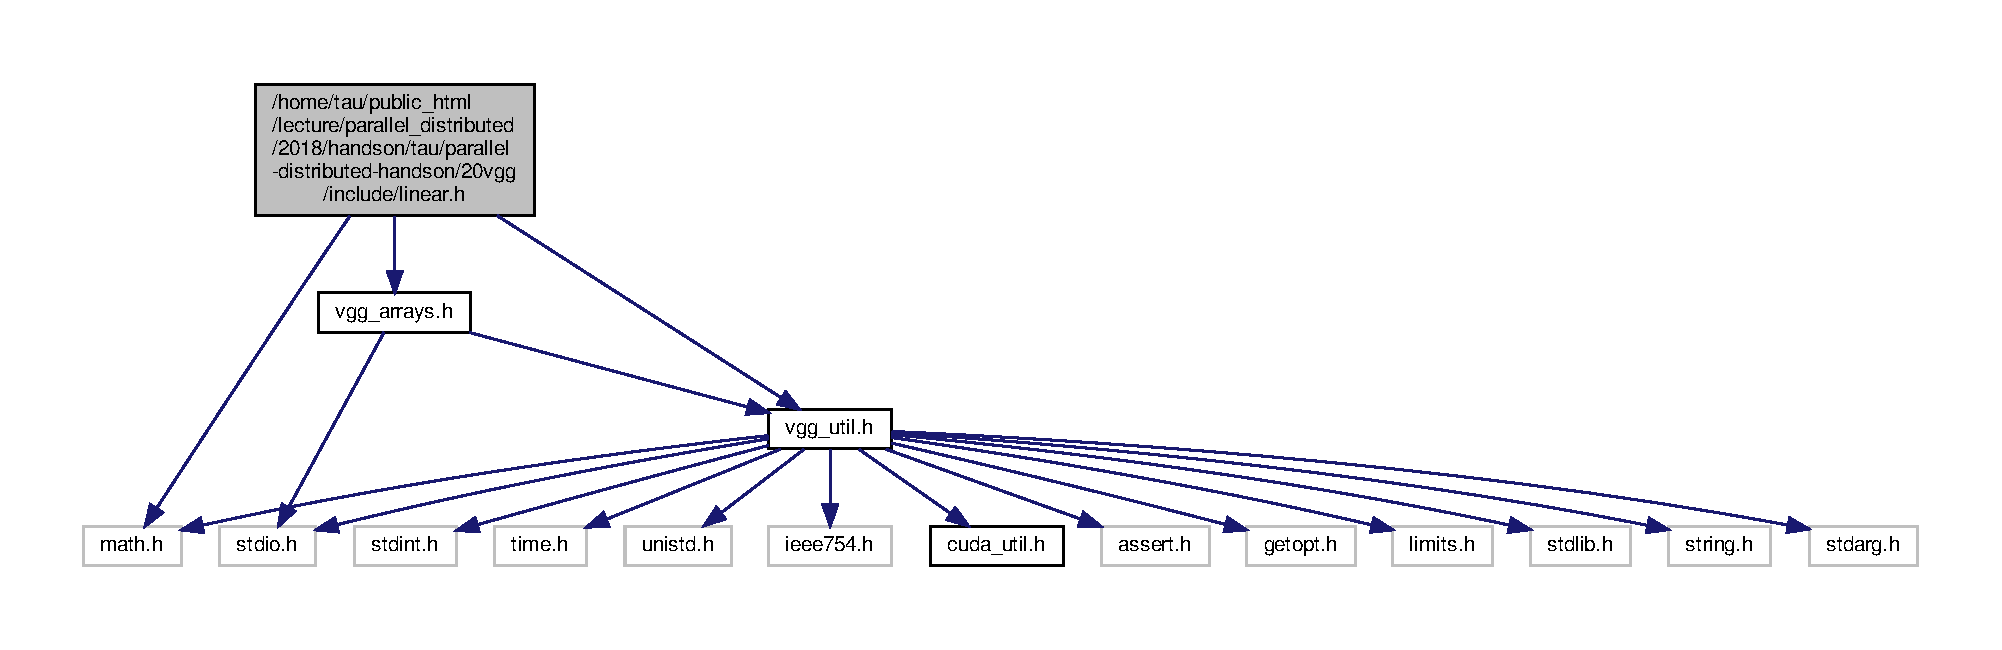
\includegraphics[width=350pt]{linear_8h__incl}
\end{center}
\end{figure}
This graph shows which files directly or indirectly include this file\+:\nopagebreak
\begin{figure}[H]
\begin{center}
\leavevmode
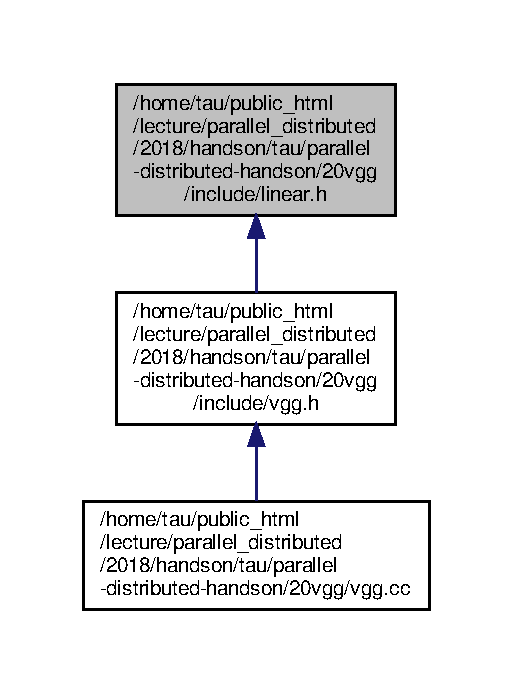
\includegraphics[width=246pt]{linear_8h__dep__incl}
\end{center}
\end{figure}
\subsection*{Classes}
\begin{DoxyCompactItemize}
\item 
struct \hyperlink{structLinear}{Linear$<$ max\+B, I\+C, n\+C $>$}
\begin{DoxyCompactList}\small\item\em linear (fully connected) layer \end{DoxyCompactList}\item 
struct \hyperlink{structLinear}{Linear$<$ max\+B, I\+C, n\+C $>$}
\begin{DoxyCompactList}\small\item\em linear (fully connected) layer \end{DoxyCompactList}\end{DoxyCompactItemize}
\subsection*{Functions}
\begin{DoxyCompactItemize}
\item 
{\footnotesize template$<$idx\+\_\+t maxB, idx\+\_\+t IC, idx\+\_\+t nC$>$ }\\\+\_\+\+\_\+global\+\_\+\+\_\+ void \hyperlink{linear_8h_a72e4feabf89d4e07eed43e83a9c9ebd0}{forward\+\_\+global} (\hyperlink{structLinear}{Linear}$<$ maxB, IC, nC $>$ $\ast$dev, \hyperlink{structarray4}{array4}$<$ maxB, IC, 1, 1 $>$ $\ast$x\+\_\+dev)
\begin{DoxyCompactList}\small\item\em a global C\+U\+DA function that implements the baseline forward function for G\+PU \end{DoxyCompactList}\item 
{\footnotesize template$<$idx\+\_\+t maxB, idx\+\_\+t IC, idx\+\_\+t nC$>$ }\\\+\_\+\+\_\+global\+\_\+\+\_\+ void \hyperlink{linear_8h_a99240505fdaa0211315f5749d0c61320}{backward\+\_\+global} (\hyperlink{structLinear}{Linear}$<$ maxB, IC, nC $>$ $\ast$dev, \hyperlink{structarray4}{array4}$<$ maxB, nC, 1, 1 $>$ $\ast$gy\+\_\+dev)
\begin{DoxyCompactList}\small\item\em a global C\+U\+DA function that implements the baseline backward function for G\+PU \end{DoxyCompactList}\item 
{\footnotesize template$<$idx\+\_\+t maxB, idx\+\_\+t IC, idx\+\_\+t nC$>$ }\\\+\_\+\+\_\+global\+\_\+\+\_\+ void \hyperlink{linear_8h_a810703be28422bb9483665cbdbafd968}{update\+\_\+global} (\hyperlink{structLinear}{Linear}$<$ maxB, IC, nC $>$ $\ast$dev, \hyperlink{vgg__util_8h_a1082d08aaa761215ec83e7149f27ad16}{real} eta)
\begin{DoxyCompactList}\small\item\em a global C\+U\+DA function that implements the baseline update function for G\+PU \end{DoxyCompactList}\item 
{\footnotesize template$<$idx\+\_\+t maxB, idx\+\_\+t IC, idx\+\_\+t nC$>$ }\\\hyperlink{vgg__util_8h_a1082d08aaa761215ec83e7149f27ad16}{real} \hyperlink{linear_8h_ae7cdd9494703205b86a32059ff049f21}{linear\+\_\+grad\+\_\+check\+\_\+rand} (\hyperlink{structcmdline__opt}{cmdline\+\_\+opt} opt, \hyperlink{structlogger}{logger} $\ast$lgr, \hyperlink{structrnd__gen__t}{rnd\+\_\+gen\+\_\+t} \&rg, \hyperlink{vgg__util_8h_a8e93478a00e685bea5e6a3f617bf03a3}{idx\+\_\+t} B)
\begin{DoxyCompactList}\small\item\em check the gradient computation of a linear layer \end{DoxyCompactList}\item 
int \hyperlink{linear_8h_a72d8c80e7ab95f113236f842c8b77937}{linear\+\_\+main} (int argc, char $\ast$$\ast$argv)
\begin{DoxyCompactList}\small\item\em entry point of this header file \end{DoxyCompactList}\end{DoxyCompactItemize}


\subsection{Detailed Description}
linear (fully connected) layer 



\subsection{Function Documentation}
\mbox{\Hypertarget{linear_8h_a99240505fdaa0211315f5749d0c61320}\label{linear_8h_a99240505fdaa0211315f5749d0c61320}} 
\index{linear.\+h@{linear.\+h}!backward\+\_\+global@{backward\+\_\+global}}
\index{backward\+\_\+global@{backward\+\_\+global}!linear.\+h@{linear.\+h}}
\subsubsection{\texorpdfstring{backward\+\_\+global()}{backward\_global()}}
{\footnotesize\ttfamily template$<$idx\+\_\+t maxB, idx\+\_\+t IC, idx\+\_\+t nC$>$ \\
\+\_\+\+\_\+global\+\_\+\+\_\+ void backward\+\_\+global (\begin{DoxyParamCaption}\item[{\hyperlink{structLinear}{Linear}$<$ maxB, IC, nC $>$ $\ast$}]{dev,  }\item[{\hyperlink{structarray4}{array4}$<$ maxB, nC, 1, 1 $>$ $\ast$}]{gy\+\_\+dev }\end{DoxyParamCaption})}



a global C\+U\+DA function that implements the baseline backward function for G\+PU 


\begin{DoxyParams}{Parameters}
{\em (dev)} & the address of the device shadow of the object \\
\hline
{\em (gy\+\_\+dev)} & the address of the device shadow of the input matrix \\
\hline
\end{DoxyParams}
\begin{DoxySeeAlso}{See also}
backward\+\_\+dev 

backward\+\_\+gpu 
\end{DoxySeeAlso}
\mbox{\Hypertarget{linear_8h_a72e4feabf89d4e07eed43e83a9c9ebd0}\label{linear_8h_a72e4feabf89d4e07eed43e83a9c9ebd0}} 
\index{linear.\+h@{linear.\+h}!forward\+\_\+global@{forward\+\_\+global}}
\index{forward\+\_\+global@{forward\+\_\+global}!linear.\+h@{linear.\+h}}
\subsubsection{\texorpdfstring{forward\+\_\+global()}{forward\_global()}}
{\footnotesize\ttfamily template$<$idx\+\_\+t maxB, idx\+\_\+t IC, idx\+\_\+t nC$>$ \\
\+\_\+\+\_\+global\+\_\+\+\_\+ void forward\+\_\+global (\begin{DoxyParamCaption}\item[{\hyperlink{structLinear}{Linear}$<$ maxB, IC, nC $>$ $\ast$}]{dev,  }\item[{\hyperlink{structarray4}{array4}$<$ maxB, IC, 1, 1 $>$ $\ast$}]{x\+\_\+dev }\end{DoxyParamCaption})}



a global C\+U\+DA function that implements the baseline forward function for G\+PU 


\begin{DoxyParams}{Parameters}
{\em (dev)} & the address of the device shadow of the object \\
\hline
{\em (x\+\_\+dev)} & the address of the device shadow of the input matrix \\
\hline
\end{DoxyParams}
\begin{DoxySeeAlso}{See also}
forward\+\_\+dev 

forward\+\_\+gpu 
\end{DoxySeeAlso}
\mbox{\Hypertarget{linear_8h_ae7cdd9494703205b86a32059ff049f21}\label{linear_8h_ae7cdd9494703205b86a32059ff049f21}} 
\index{linear.\+h@{linear.\+h}!linear\+\_\+grad\+\_\+check\+\_\+rand@{linear\+\_\+grad\+\_\+check\+\_\+rand}}
\index{linear\+\_\+grad\+\_\+check\+\_\+rand@{linear\+\_\+grad\+\_\+check\+\_\+rand}!linear.\+h@{linear.\+h}}
\subsubsection{\texorpdfstring{linear\+\_\+grad\+\_\+check\+\_\+rand()}{linear\_grad\_check\_rand()}}
{\footnotesize\ttfamily template$<$idx\+\_\+t maxB, idx\+\_\+t IC, idx\+\_\+t nC$>$ \\
\hyperlink{vgg__util_8h_a1082d08aaa761215ec83e7149f27ad16}{real} linear\+\_\+grad\+\_\+check\+\_\+rand (\begin{DoxyParamCaption}\item[{\hyperlink{structcmdline__opt}{cmdline\+\_\+opt}}]{opt,  }\item[{\hyperlink{structlogger}{logger} $\ast$}]{lgr,  }\item[{\hyperlink{structrnd__gen__t}{rnd\+\_\+gen\+\_\+t} \&}]{rg,  }\item[{\hyperlink{vgg__util_8h_a8e93478a00e685bea5e6a3f617bf03a3}{idx\+\_\+t}}]{B }\end{DoxyParamCaption})}



check the gradient computation of a linear layer 


\begin{DoxyParams}{Parameters}
{\em (opt)} & command line option \\
\hline
{\em (lgr)} & logger \\
\hline
{\em (rg)} & random number generator \\
\hline
{\em (\+B)} & the number of images \\
\hline
\end{DoxyParams}
\begin{DoxySeeAlso}{See also}
\hyperlink{linear_8h_a72d8c80e7ab95f113236f842c8b77937}{linear\+\_\+main}
\end{DoxySeeAlso}
it first makes a layer object with initial weights W and generates an input (x and t). it then creates two layers whose weights are slightly different from the original one by dw/2 (i.\+e., w-\/dw/2 and w+dw/2), as well as two inputs slighly different from the original inputs by dx/2 (x-\/dx/2 and x+dx/2). it then computes L(w,x), L(x-\/dw/2,x-\/dx/2) and L(w+dw/2,x+dw/2) and check if L(x+dw/2,x+dx/2)-\/L(x-\/dw/2,x-\/dx/2) is close to ∂\+L/∂x dx + ∂\+L/∂w dw. ∂\+L/∂x and ∂\+L/∂w are obtained by backward computation. This is essentially checking if the gradients obtained by backward computation correctly approximates the diff of the output. \mbox{\Hypertarget{linear_8h_a72d8c80e7ab95f113236f842c8b77937}\label{linear_8h_a72d8c80e7ab95f113236f842c8b77937}} 
\index{linear.\+h@{linear.\+h}!linear\+\_\+main@{linear\+\_\+main}}
\index{linear\+\_\+main@{linear\+\_\+main}!linear.\+h@{linear.\+h}}
\subsubsection{\texorpdfstring{linear\+\_\+main()}{linear\_main()}}
{\footnotesize\ttfamily int linear\+\_\+main (\begin{DoxyParamCaption}\item[{int}]{argc,  }\item[{char $\ast$$\ast$}]{argv }\end{DoxyParamCaption})}



entry point of this header file 


\begin{DoxyParams}{Parameters}
{\em (argc)} & the number of command line args \\
\hline
{\em (argv)} & command line args \\
\hline
\end{DoxyParams}
\begin{DoxySeeAlso}{See also}
\hyperlink{linear_8h_ae7cdd9494703205b86a32059ff049f21}{linear\+\_\+grad\+\_\+check\+\_\+rand}
\end{DoxySeeAlso}
if this header file is included from a main C++ file and define linear\+\_\+main to be main (e.\+g., with -\/\+Dlinear\+\_\+main=main), then this function becomes th main function of the executable. it calls linear\+\_\+grad\+\_\+check\+\_\+rand repeatedly to test the implementation of \hyperlink{structVGG}{V\+GG} network. \mbox{\Hypertarget{linear_8h_a810703be28422bb9483665cbdbafd968}\label{linear_8h_a810703be28422bb9483665cbdbafd968}} 
\index{linear.\+h@{linear.\+h}!update\+\_\+global@{update\+\_\+global}}
\index{update\+\_\+global@{update\+\_\+global}!linear.\+h@{linear.\+h}}
\subsubsection{\texorpdfstring{update\+\_\+global()}{update\_global()}}
{\footnotesize\ttfamily template$<$idx\+\_\+t maxB, idx\+\_\+t IC, idx\+\_\+t nC$>$ \\
\+\_\+\+\_\+global\+\_\+\+\_\+ void update\+\_\+global (\begin{DoxyParamCaption}\item[{\hyperlink{structLinear}{Linear}$<$ maxB, IC, nC $>$ $\ast$}]{dev,  }\item[{\hyperlink{vgg__util_8h_a1082d08aaa761215ec83e7149f27ad16}{real}}]{eta }\end{DoxyParamCaption})}



a global C\+U\+DA function that implements the baseline update function for G\+PU 


\begin{DoxyParams}{Parameters}
{\em (dev)} & the address of the device shadow of the object \\
\hline
{\em (eta)} & the address of the device shadow of the input matrix \\
\hline
\end{DoxyParams}
\begin{DoxySeeAlso}{See also}
update\+\_\+dev 

update\+\_\+gpu 
\end{DoxySeeAlso}

\hypertarget{maxpooling_8h}{}\section{/home/tau/public\+\_\+html/lecture/parallel\+\_\+distributed/2018/handson/tau/parallel-\/distributed-\/handson/20vgg/include/maxpooling.h File Reference}
\label{maxpooling_8h}\index{/home/tau/public\+\_\+html/lecture/parallel\+\_\+distributed/2018/handson/tau/parallel-\/distributed-\/handson/20vgg/include/maxpooling.\+h@{/home/tau/public\+\_\+html/lecture/parallel\+\_\+distributed/2018/handson/tau/parallel-\/distributed-\/handson/20vgg/include/maxpooling.\+h}}


max pooling layer  


{\ttfamily \#include \char`\"{}vgg\+\_\+util.\+h\char`\"{}}\newline
{\ttfamily \#include \char`\"{}vgg\+\_\+arrays.\+h\char`\"{}}\newline
Include dependency graph for maxpooling.\+h\+:\nopagebreak
\begin{figure}[H]
\begin{center}
\leavevmode
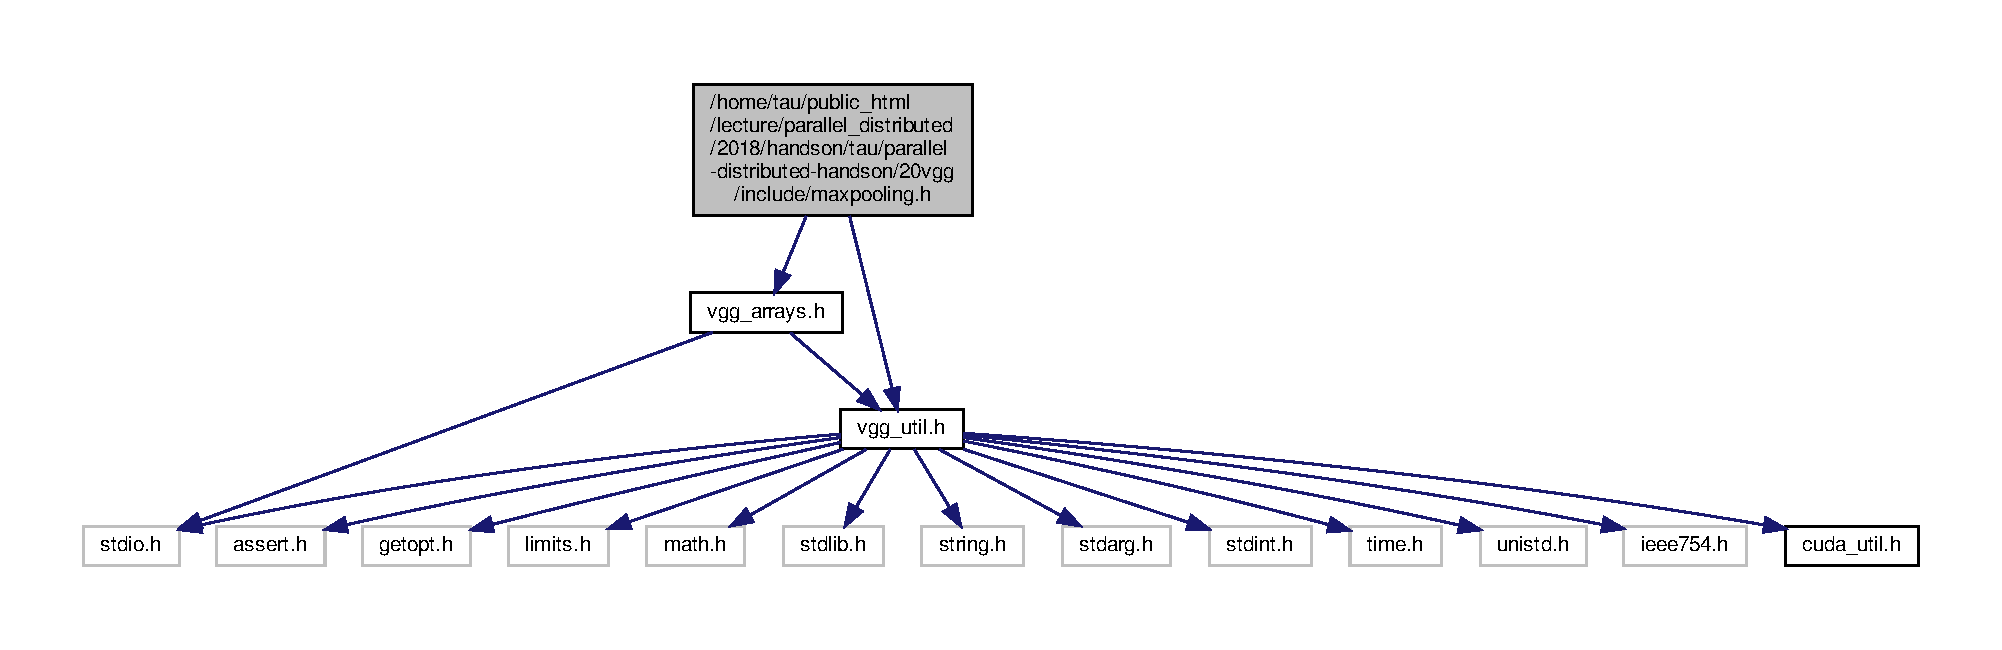
\includegraphics[width=350pt]{maxpooling_8h__incl}
\end{center}
\end{figure}
This graph shows which files directly or indirectly include this file\+:\nopagebreak
\begin{figure}[H]
\begin{center}
\leavevmode
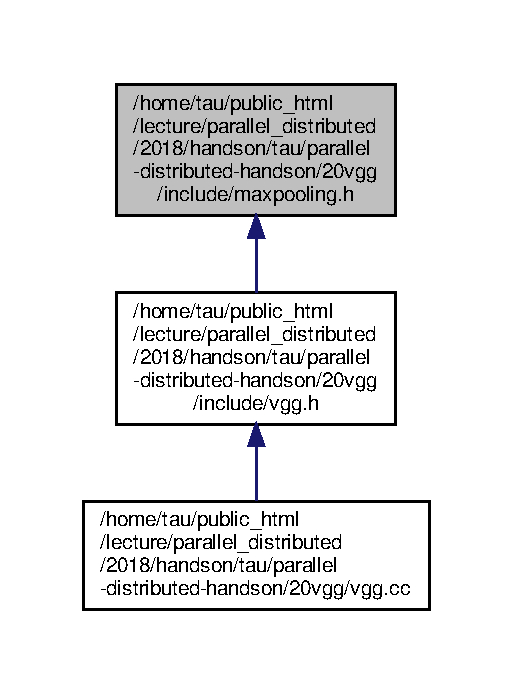
\includegraphics[width=246pt]{maxpooling_8h__dep__incl}
\end{center}
\end{figure}
\subsection*{Classes}
\begin{DoxyCompactItemize}
\item 
struct \hyperlink{structMaxPooling2D}{Max\+Pooling2\+D$<$ max\+B, C, H, W, S $>$}
\begin{DoxyCompactList}\small\item\em max pooling layer \end{DoxyCompactList}\item 
struct \hyperlink{structMaxPooling2D}{Max\+Pooling2\+D$<$ max\+B, C, H, W, S $>$}
\begin{DoxyCompactList}\small\item\em max pooling layer \end{DoxyCompactList}\end{DoxyCompactItemize}
\subsection*{Functions}
\begin{DoxyCompactItemize}
\item 
{\footnotesize template$<$idx\+\_\+t maxB, idx\+\_\+t C, idx\+\_\+t H, idx\+\_\+t W, idx\+\_\+t S$>$ }\\\+\_\+\+\_\+global\+\_\+\+\_\+ void \hyperlink{maxpooling_8h_a86284783b27527773adb05dc5f9c59f5}{forward\+\_\+global} (\hyperlink{structMaxPooling2D}{Max\+Pooling2D}$<$ maxB, C, H, W, S $>$ $\ast$dev, \hyperlink{structarray4}{array4}$<$ maxB, C, H, W $>$ $\ast$x\+\_\+dev)
\begin{DoxyCompactList}\small\item\em a global C\+U\+DA function that implements the baseline forward function for G\+PU \end{DoxyCompactList}\item 
{\footnotesize template$<$idx\+\_\+t maxB, idx\+\_\+t C, idx\+\_\+t H, idx\+\_\+t W, idx\+\_\+t S$>$ }\\\+\_\+\+\_\+global\+\_\+\+\_\+ void \hyperlink{maxpooling_8h_af53c5ee034d70078735159eec7767455}{backward\+\_\+global} (\hyperlink{structMaxPooling2D}{Max\+Pooling2D}$<$ maxB, C, H, W, S $>$ $\ast$dev, \hyperlink{structarray4}{array4}$<$ maxB, C, H/S, W/S $>$ $\ast$gy\+\_\+dev)
\begin{DoxyCompactList}\small\item\em a global C\+U\+DA function that implements the baseline backward function for G\+PU \end{DoxyCompactList}\item 
{\footnotesize template$<$idx\+\_\+t maxB, idx\+\_\+t C, idx\+\_\+t H, idx\+\_\+t W, idx\+\_\+t S$>$ }\\\hyperlink{vgg__util_8h_a1082d08aaa761215ec83e7149f27ad16}{real} \hyperlink{maxpooling_8h_ae1be032747b4c558424af53ca04805bd}{maxpooling\+\_\+grad\+\_\+check\+\_\+rand} (\hyperlink{structcmdline__opt}{cmdline\+\_\+opt} opt, \hyperlink{structlogger}{logger} $\ast$lgr, \hyperlink{structrnd__gen__t}{rnd\+\_\+gen\+\_\+t} \&rg, \hyperlink{vgg__util_8h_a8e93478a00e685bea5e6a3f617bf03a3}{idx\+\_\+t} B)
\begin{DoxyCompactList}\small\item\em check the gradient computation of a maxpooling layer \end{DoxyCompactList}\item 
int \hyperlink{maxpooling_8h_afeaa2cae881fd24885faca831920c4da}{maxpooling\+\_\+main} (int argc, char $\ast$$\ast$argv)
\begin{DoxyCompactList}\small\item\em entry point of this header file \end{DoxyCompactList}\end{DoxyCompactItemize}


\subsection{Detailed Description}
max pooling layer 



\subsection{Function Documentation}
\mbox{\Hypertarget{maxpooling_8h_af53c5ee034d70078735159eec7767455}\label{maxpooling_8h_af53c5ee034d70078735159eec7767455}} 
\index{maxpooling.\+h@{maxpooling.\+h}!backward\+\_\+global@{backward\+\_\+global}}
\index{backward\+\_\+global@{backward\+\_\+global}!maxpooling.\+h@{maxpooling.\+h}}
\subsubsection{\texorpdfstring{backward\+\_\+global()}{backward\_global()}}
{\footnotesize\ttfamily template$<$idx\+\_\+t maxB, idx\+\_\+t C, idx\+\_\+t H, idx\+\_\+t W, idx\+\_\+t S$>$ \\
\+\_\+\+\_\+global\+\_\+\+\_\+ void backward\+\_\+global (\begin{DoxyParamCaption}\item[{\hyperlink{structMaxPooling2D}{Max\+Pooling2D}$<$ maxB, C, H, W, S $>$ $\ast$}]{dev,  }\item[{\hyperlink{structarray4}{array4}$<$ maxB, C, H/S, W/S $>$ $\ast$}]{gy\+\_\+dev }\end{DoxyParamCaption})}



a global C\+U\+DA function that implements the baseline backward function for G\+PU 


\begin{DoxyParams}{Parameters}
{\em (dev)} & the address of the device shadow of the object \\
\hline
{\em (gy\+\_\+dev)} & the address of the device shadow of the input matrix \\
\hline
\end{DoxyParams}
\begin{DoxySeeAlso}{See also}
backward\+\_\+dev 

backward\+\_\+gpu 
\end{DoxySeeAlso}
\mbox{\Hypertarget{maxpooling_8h_a86284783b27527773adb05dc5f9c59f5}\label{maxpooling_8h_a86284783b27527773adb05dc5f9c59f5}} 
\index{maxpooling.\+h@{maxpooling.\+h}!forward\+\_\+global@{forward\+\_\+global}}
\index{forward\+\_\+global@{forward\+\_\+global}!maxpooling.\+h@{maxpooling.\+h}}
\subsubsection{\texorpdfstring{forward\+\_\+global()}{forward\_global()}}
{\footnotesize\ttfamily template$<$idx\+\_\+t maxB, idx\+\_\+t C, idx\+\_\+t H, idx\+\_\+t W, idx\+\_\+t S$>$ \\
\+\_\+\+\_\+global\+\_\+\+\_\+ void forward\+\_\+global (\begin{DoxyParamCaption}\item[{\hyperlink{structMaxPooling2D}{Max\+Pooling2D}$<$ maxB, C, H, W, S $>$ $\ast$}]{dev,  }\item[{\hyperlink{structarray4}{array4}$<$ maxB, C, H, W $>$ $\ast$}]{x\+\_\+dev }\end{DoxyParamCaption})}



a global C\+U\+DA function that implements the baseline forward function for G\+PU 


\begin{DoxyParams}{Parameters}
{\em (dev)} & the address of the device shadow of the object \\
\hline
{\em (x\+\_\+dev)} & the address of the device shadow of the input matrix \\
\hline
\end{DoxyParams}
\begin{DoxySeeAlso}{See also}
forward\+\_\+dev 

forward\+\_\+gpu 
\end{DoxySeeAlso}
\mbox{\Hypertarget{maxpooling_8h_ae1be032747b4c558424af53ca04805bd}\label{maxpooling_8h_ae1be032747b4c558424af53ca04805bd}} 
\index{maxpooling.\+h@{maxpooling.\+h}!maxpooling\+\_\+grad\+\_\+check\+\_\+rand@{maxpooling\+\_\+grad\+\_\+check\+\_\+rand}}
\index{maxpooling\+\_\+grad\+\_\+check\+\_\+rand@{maxpooling\+\_\+grad\+\_\+check\+\_\+rand}!maxpooling.\+h@{maxpooling.\+h}}
\subsubsection{\texorpdfstring{maxpooling\+\_\+grad\+\_\+check\+\_\+rand()}{maxpooling\_grad\_check\_rand()}}
{\footnotesize\ttfamily template$<$idx\+\_\+t maxB, idx\+\_\+t C, idx\+\_\+t H, idx\+\_\+t W, idx\+\_\+t S$>$ \\
\hyperlink{vgg__util_8h_a1082d08aaa761215ec83e7149f27ad16}{real} maxpooling\+\_\+grad\+\_\+check\+\_\+rand (\begin{DoxyParamCaption}\item[{\hyperlink{structcmdline__opt}{cmdline\+\_\+opt}}]{opt,  }\item[{\hyperlink{structlogger}{logger} $\ast$}]{lgr,  }\item[{\hyperlink{structrnd__gen__t}{rnd\+\_\+gen\+\_\+t} \&}]{rg,  }\item[{\hyperlink{vgg__util_8h_a8e93478a00e685bea5e6a3f617bf03a3}{idx\+\_\+t}}]{B }\end{DoxyParamCaption})}



check the gradient computation of a maxpooling layer 


\begin{DoxyParams}{Parameters}
{\em (opt)} & command line option \\
\hline
{\em (lgr)} & logger \\
\hline
{\em (rg)} & random number generator \\
\hline
{\em (\+B)} & the number of images \\
\hline
\end{DoxyParams}
\begin{DoxySeeAlso}{See also}
\hyperlink{maxpooling_8h_afeaa2cae881fd24885faca831920c4da}{maxpooling\+\_\+main}
\end{DoxySeeAlso}
it first makes a layer object with initial weights W and generates an input (x and t). it then creates two layers whose weights are slightly different from the original one by dw/2 (i.\+e., w-\/dw/2 and w+dw/2), as well as two inputs slighly different from the original inputs by dx/2 (x-\/dx/2 and x+dx/2). it then computes L(w,x), L(x-\/dw/2,x-\/dx/2) and L(w+dw/2,x+dw/2) and check if L(x+dw/2,x+dx/2)-\/L(x-\/dw/2,x-\/dx/2) is close to ∂\+L/∂x dx + ∂\+L/∂w dw. ∂\+L/∂x and ∂\+L/∂w are obtained by backward computation. This is essentially checking if the gradients obtained by backward computation correctly approximates the diff of the output. \mbox{\Hypertarget{maxpooling_8h_afeaa2cae881fd24885faca831920c4da}\label{maxpooling_8h_afeaa2cae881fd24885faca831920c4da}} 
\index{maxpooling.\+h@{maxpooling.\+h}!maxpooling\+\_\+main@{maxpooling\+\_\+main}}
\index{maxpooling\+\_\+main@{maxpooling\+\_\+main}!maxpooling.\+h@{maxpooling.\+h}}
\subsubsection{\texorpdfstring{maxpooling\+\_\+main()}{maxpooling\_main()}}
{\footnotesize\ttfamily int maxpooling\+\_\+main (\begin{DoxyParamCaption}\item[{int}]{argc,  }\item[{char $\ast$$\ast$}]{argv }\end{DoxyParamCaption})}



entry point of this header file 


\begin{DoxyParams}{Parameters}
{\em (argc)} & the number of command line args \\
\hline
{\em (argv)} & command line args \\
\hline
\end{DoxyParams}
\begin{DoxySeeAlso}{See also}
\hyperlink{maxpooling_8h_ae1be032747b4c558424af53ca04805bd}{maxpooling\+\_\+grad\+\_\+check\+\_\+rand}
\end{DoxySeeAlso}
if this header file is included from a main C++ file and define maxpooling\+\_\+main to be main (e.\+g., with -\/\+Dmaxpooling\+\_\+main=main), then this function becomes th main function of the executable. it calls maxpooling\+\_\+grad\+\_\+check\+\_\+rand repeatedly to test the implementation of \hyperlink{structVGG}{V\+GG} network. 
\hypertarget{relu_8h}{}\section{/home/tau/public\+\_\+html/lecture/parallel\+\_\+distributed/2018/handson/tau/parallel-\/distributed-\/handson/20vgg/include/relu.h File Reference}
\label{relu_8h}\index{/home/tau/public\+\_\+html/lecture/parallel\+\_\+distributed/2018/handson/tau/parallel-\/distributed-\/handson/20vgg/include/relu.\+h@{/home/tau/public\+\_\+html/lecture/parallel\+\_\+distributed/2018/handson/tau/parallel-\/distributed-\/handson/20vgg/include/relu.\+h}}


rectified linear activation layer (relu(x) = max(0,x))  


{\ttfamily \#include \char`\"{}vgg\+\_\+util.\+h\char`\"{}}\newline
{\ttfamily \#include \char`\"{}vgg\+\_\+arrays.\+h\char`\"{}}\newline
Include dependency graph for relu.\+h\+:\nopagebreak
\begin{figure}[H]
\begin{center}
\leavevmode
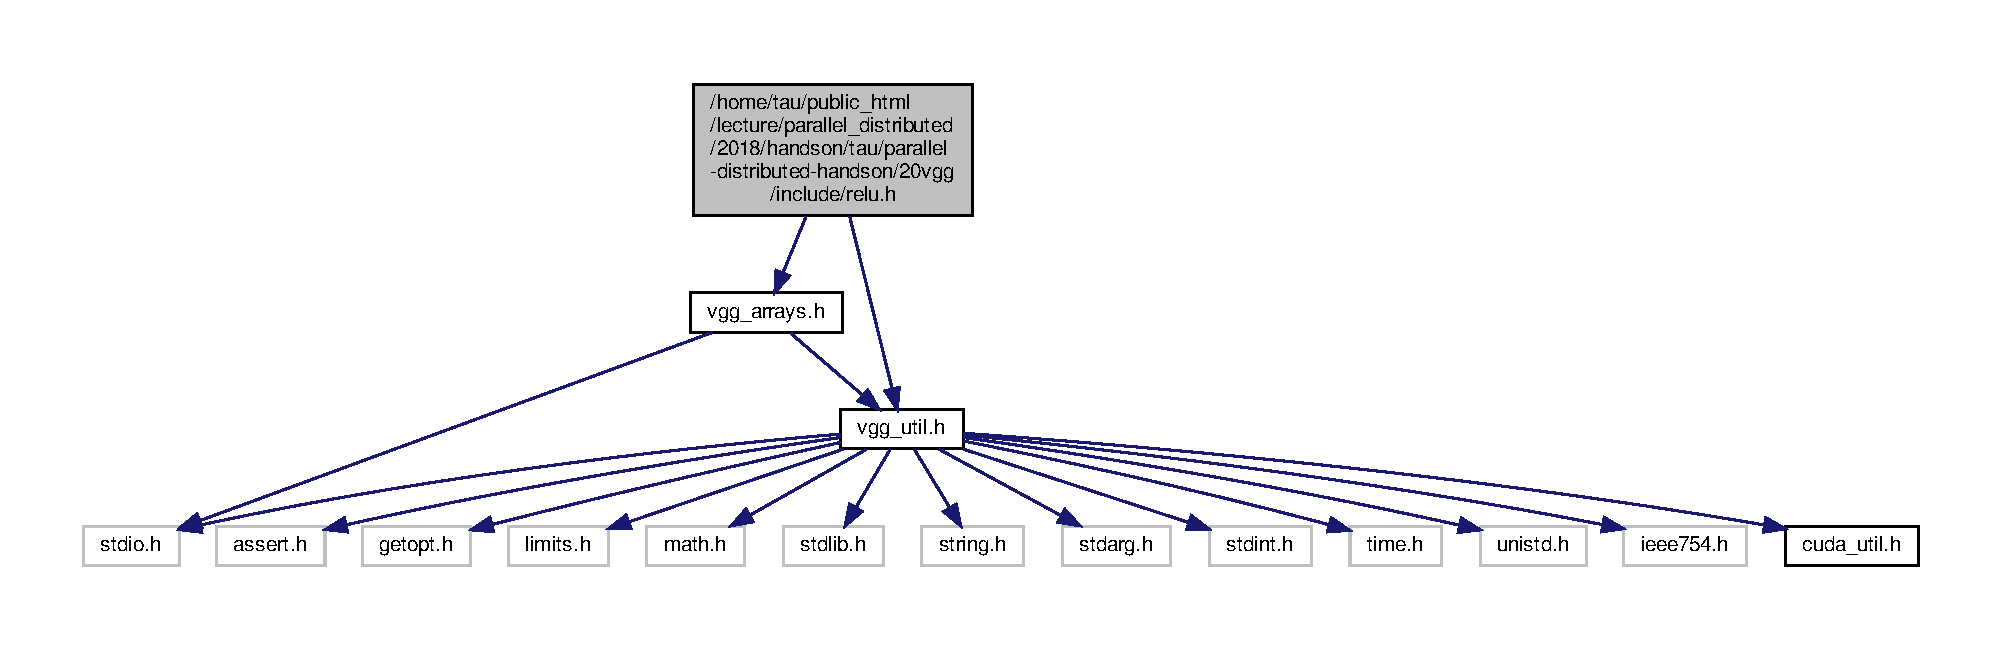
\includegraphics[width=350pt]{relu_8h__incl}
\end{center}
\end{figure}
This graph shows which files directly or indirectly include this file\+:\nopagebreak
\begin{figure}[H]
\begin{center}
\leavevmode
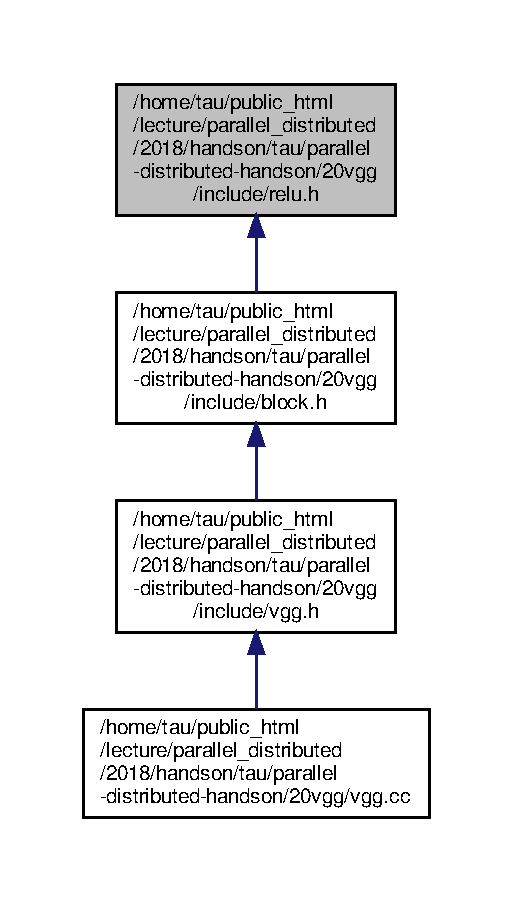
\includegraphics[width=246pt]{relu_8h__dep__incl}
\end{center}
\end{figure}
\subsection*{Classes}
\begin{DoxyCompactItemize}
\item 
struct \hyperlink{structRelu}{Relu$<$ max\+B, C, H, W $>$}
\begin{DoxyCompactList}\small\item\em dropout layer \end{DoxyCompactList}\item 
struct \hyperlink{structRelu}{Relu$<$ max\+B, C, H, W $>$}
\begin{DoxyCompactList}\small\item\em dropout layer \end{DoxyCompactList}\end{DoxyCompactItemize}
\subsection*{Functions}
\begin{DoxyCompactItemize}
\item 
{\footnotesize template$<$idx\+\_\+t maxB, idx\+\_\+t C, idx\+\_\+t H, idx\+\_\+t W$>$ }\\\+\_\+\+\_\+global\+\_\+\+\_\+ void \hyperlink{relu_8h_ab66f883c0c48ee470eea00e1e312b4b7}{forward\+\_\+global} (\hyperlink{structRelu}{Relu}$<$ maxB, C, H, W $>$ $\ast$dev, \hyperlink{structarray4}{array4}$<$ maxB, C, H, W $>$ $\ast$x\+\_\+dev)
\begin{DoxyCompactList}\small\item\em a global C\+U\+DA function that implements the baseline forward function for G\+PU \end{DoxyCompactList}\item 
{\footnotesize template$<$idx\+\_\+t maxB, idx\+\_\+t C, idx\+\_\+t H, idx\+\_\+t W$>$ }\\\+\_\+\+\_\+global\+\_\+\+\_\+ void \hyperlink{relu_8h_a6f9d52164079bacd6aad2e984fa68de8}{backward\+\_\+global} (\hyperlink{structRelu}{Relu}$<$ maxB, C, H, W $>$ $\ast$dev, \hyperlink{structarray4}{array4}$<$ maxB, C, H, W $>$ $\ast$gy\+\_\+dev)
\begin{DoxyCompactList}\small\item\em a global C\+U\+DA function that implements the baseline backward function for G\+PU \end{DoxyCompactList}\item 
{\footnotesize template$<$idx\+\_\+t maxB, idx\+\_\+t C, idx\+\_\+t H, idx\+\_\+t W$>$ }\\static \hyperlink{vgg__util_8h_a1082d08aaa761215ec83e7149f27ad16}{real} \hyperlink{relu_8h_ac2d23da00a0aabbd4cfde6833ba431c3}{relu\+\_\+grad\+\_\+check\+\_\+rand} (\hyperlink{structcmdline__opt}{cmdline\+\_\+opt} opt, \hyperlink{structlogger}{logger} $\ast$lgr, \hyperlink{structrnd__gen__t}{rnd\+\_\+gen\+\_\+t} \&rg, \hyperlink{vgg__util_8h_a8e93478a00e685bea5e6a3f617bf03a3}{idx\+\_\+t} B)
\begin{DoxyCompactList}\small\item\em check the gradient computation of a relu layer \end{DoxyCompactList}\item 
int \hyperlink{relu_8h_a4799d44fc9419d0a9259cb57d45995a9}{relu\+\_\+main} (int argc, char $\ast$$\ast$argv)
\begin{DoxyCompactList}\small\item\em entry point of this header file \end{DoxyCompactList}\end{DoxyCompactItemize}


\subsection{Detailed Description}
rectified linear activation layer (relu(x) = max(0,x)) 



\subsection{Function Documentation}
\mbox{\Hypertarget{relu_8h_a6f9d52164079bacd6aad2e984fa68de8}\label{relu_8h_a6f9d52164079bacd6aad2e984fa68de8}} 
\index{relu.\+h@{relu.\+h}!backward\+\_\+global@{backward\+\_\+global}}
\index{backward\+\_\+global@{backward\+\_\+global}!relu.\+h@{relu.\+h}}
\subsubsection{\texorpdfstring{backward\+\_\+global()}{backward\_global()}}
{\footnotesize\ttfamily template$<$idx\+\_\+t maxB, idx\+\_\+t C, idx\+\_\+t H, idx\+\_\+t W$>$ \\
\+\_\+\+\_\+global\+\_\+\+\_\+ void backward\+\_\+global (\begin{DoxyParamCaption}\item[{\hyperlink{structRelu}{Relu}$<$ maxB, C, H, W $>$ $\ast$}]{dev,  }\item[{\hyperlink{structarray4}{array4}$<$ maxB, C, H, W $>$ $\ast$}]{gy\+\_\+dev }\end{DoxyParamCaption})}



a global C\+U\+DA function that implements the baseline backward function for G\+PU 


\begin{DoxyParams}{Parameters}
{\em (dev)} & the address of the device shadow of the object \\
\hline
{\em (gy\+\_\+dev)} & the address of the device shadow of the input matrix \\
\hline
\end{DoxyParams}
\begin{DoxySeeAlso}{See also}
backward\+\_\+dev 

backward\+\_\+gpu 
\end{DoxySeeAlso}
\mbox{\Hypertarget{relu_8h_ab66f883c0c48ee470eea00e1e312b4b7}\label{relu_8h_ab66f883c0c48ee470eea00e1e312b4b7}} 
\index{relu.\+h@{relu.\+h}!forward\+\_\+global@{forward\+\_\+global}}
\index{forward\+\_\+global@{forward\+\_\+global}!relu.\+h@{relu.\+h}}
\subsubsection{\texorpdfstring{forward\+\_\+global()}{forward\_global()}}
{\footnotesize\ttfamily template$<$idx\+\_\+t maxB, idx\+\_\+t C, idx\+\_\+t H, idx\+\_\+t W$>$ \\
\+\_\+\+\_\+global\+\_\+\+\_\+ void forward\+\_\+global (\begin{DoxyParamCaption}\item[{\hyperlink{structRelu}{Relu}$<$ maxB, C, H, W $>$ $\ast$}]{dev,  }\item[{\hyperlink{structarray4}{array4}$<$ maxB, C, H, W $>$ $\ast$}]{x\+\_\+dev }\end{DoxyParamCaption})}



a global C\+U\+DA function that implements the baseline forward function for G\+PU 


\begin{DoxyParams}{Parameters}
{\em (dev)} & the address of the device shadow of the object \\
\hline
{\em (x\+\_\+dev)} & the address of the device shadow of the input matrix \\
\hline
\end{DoxyParams}
\begin{DoxySeeAlso}{See also}
forward\+\_\+dev 

forward\+\_\+gpu 
\end{DoxySeeAlso}
\mbox{\Hypertarget{relu_8h_ac2d23da00a0aabbd4cfde6833ba431c3}\label{relu_8h_ac2d23da00a0aabbd4cfde6833ba431c3}} 
\index{relu.\+h@{relu.\+h}!relu\+\_\+grad\+\_\+check\+\_\+rand@{relu\+\_\+grad\+\_\+check\+\_\+rand}}
\index{relu\+\_\+grad\+\_\+check\+\_\+rand@{relu\+\_\+grad\+\_\+check\+\_\+rand}!relu.\+h@{relu.\+h}}
\subsubsection{\texorpdfstring{relu\+\_\+grad\+\_\+check\+\_\+rand()}{relu\_grad\_check\_rand()}}
{\footnotesize\ttfamily template$<$idx\+\_\+t maxB, idx\+\_\+t C, idx\+\_\+t H, idx\+\_\+t W$>$ \\
static \hyperlink{vgg__util_8h_a1082d08aaa761215ec83e7149f27ad16}{real} relu\+\_\+grad\+\_\+check\+\_\+rand (\begin{DoxyParamCaption}\item[{\hyperlink{structcmdline__opt}{cmdline\+\_\+opt}}]{opt,  }\item[{\hyperlink{structlogger}{logger} $\ast$}]{lgr,  }\item[{\hyperlink{structrnd__gen__t}{rnd\+\_\+gen\+\_\+t} \&}]{rg,  }\item[{\hyperlink{vgg__util_8h_a8e93478a00e685bea5e6a3f617bf03a3}{idx\+\_\+t}}]{B }\end{DoxyParamCaption})\hspace{0.3cm}{\ttfamily [static]}}



check the gradient computation of a relu layer 


\begin{DoxyParams}{Parameters}
{\em (opt)} & command line option \\
\hline
{\em (lgr)} & logger \\
\hline
{\em (rg)} & random number generator \\
\hline
{\em (\+B)} & the number of images \\
\hline
\end{DoxyParams}
\begin{DoxySeeAlso}{See also}
\hyperlink{relu_8h_a4799d44fc9419d0a9259cb57d45995a9}{relu\+\_\+main}
\end{DoxySeeAlso}
it first makes a layer object with initial weights W and generates an input (x and t). it then creates two layers whose weights are slightly different from the original one by dw/2 (i.\+e., w-\/dw/2 and w+dw/2), as well as two inputs slighly different from the original inputs by dx/2 (x-\/dx/2 and x+dx/2). it then computes L(w,x), L(x-\/dw/2,x-\/dx/2) and L(w+dw/2,x+dw/2) and check if L(x+dw/2,x+dx/2)-\/L(x-\/dw/2,x-\/dx/2) is close to ∂\+L/∂x dx + ∂\+L/∂w dw. ∂\+L/∂x and ∂\+L/∂w are obtained by backward computation. This is essentially checking if the gradients obtained by backward computation correctly approximates the diff of the output. \mbox{\Hypertarget{relu_8h_a4799d44fc9419d0a9259cb57d45995a9}\label{relu_8h_a4799d44fc9419d0a9259cb57d45995a9}} 
\index{relu.\+h@{relu.\+h}!relu\+\_\+main@{relu\+\_\+main}}
\index{relu\+\_\+main@{relu\+\_\+main}!relu.\+h@{relu.\+h}}
\subsubsection{\texorpdfstring{relu\+\_\+main()}{relu\_main()}}
{\footnotesize\ttfamily int relu\+\_\+main (\begin{DoxyParamCaption}\item[{int}]{argc,  }\item[{char $\ast$$\ast$}]{argv }\end{DoxyParamCaption})}



entry point of this header file 


\begin{DoxyParams}{Parameters}
{\em (argc)} & the number of command line args \\
\hline
{\em (argv)} & command line args \\
\hline
\end{DoxyParams}
\begin{DoxySeeAlso}{See also}
\hyperlink{relu_8h_ac2d23da00a0aabbd4cfde6833ba431c3}{relu\+\_\+grad\+\_\+check\+\_\+rand}
\end{DoxySeeAlso}
if this header file is included from a main C++ file and define relu\+\_\+main to be main (e.\+g., with -\/\+Drelu\+\_\+main=main), then this function becomes th main function of the executable. it calls relu\+\_\+grad\+\_\+check\+\_\+rand repeatedly to test the implementation of \hyperlink{structVGG}{V\+GG} network. 
\hypertarget{softmaxcrossentropy_8h}{}\section{/home/tau/public\+\_\+html/lecture/parallel\+\_\+distributed/2018/handson/tau/parallel-\/distributed-\/handson/20vgg/include/softmaxcrossentropy.h File Reference}
\label{softmaxcrossentropy_8h}\index{/home/tau/public\+\_\+html/lecture/parallel\+\_\+distributed/2018/handson/tau/parallel-\/distributed-\/handson/20vgg/include/softmaxcrossentropy.\+h@{/home/tau/public\+\_\+html/lecture/parallel\+\_\+distributed/2018/handson/tau/parallel-\/distributed-\/handson/20vgg/include/softmaxcrossentropy.\+h}}


softmax + cross entropy layer  


{\ttfamily \#include $<$math.\+h$>$}\newline
{\ttfamily \#include \char`\"{}vgg\+\_\+util.\+h\char`\"{}}\newline
{\ttfamily \#include \char`\"{}vgg\+\_\+arrays.\+h\char`\"{}}\newline
Include dependency graph for softmaxcrossentropy.\+h\+:\nopagebreak
\begin{figure}[H]
\begin{center}
\leavevmode
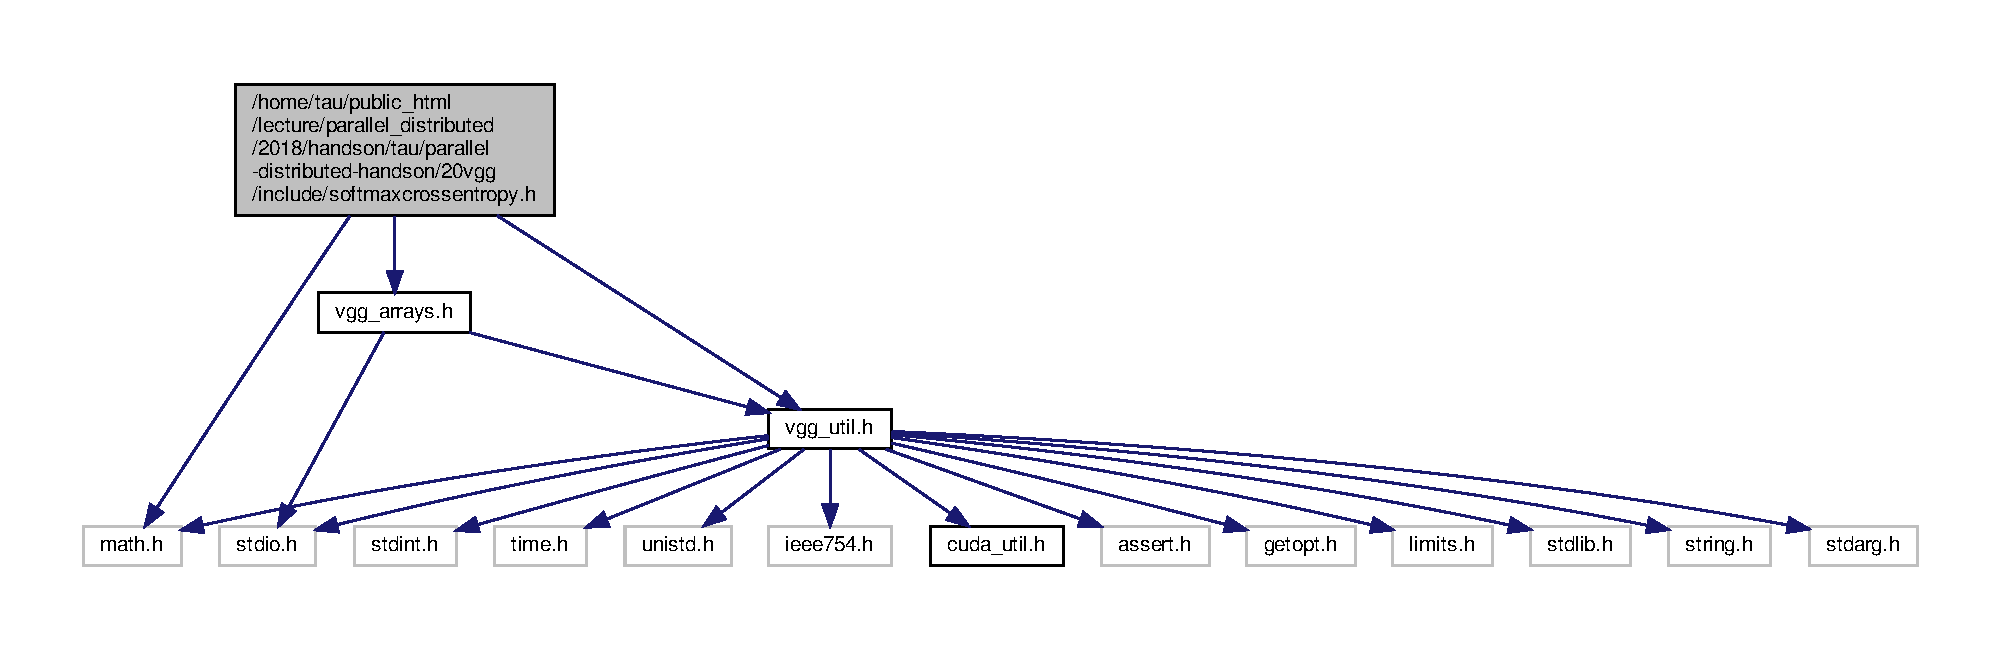
\includegraphics[width=350pt]{softmaxcrossentropy_8h__incl}
\end{center}
\end{figure}
This graph shows which files directly or indirectly include this file\+:\nopagebreak
\begin{figure}[H]
\begin{center}
\leavevmode
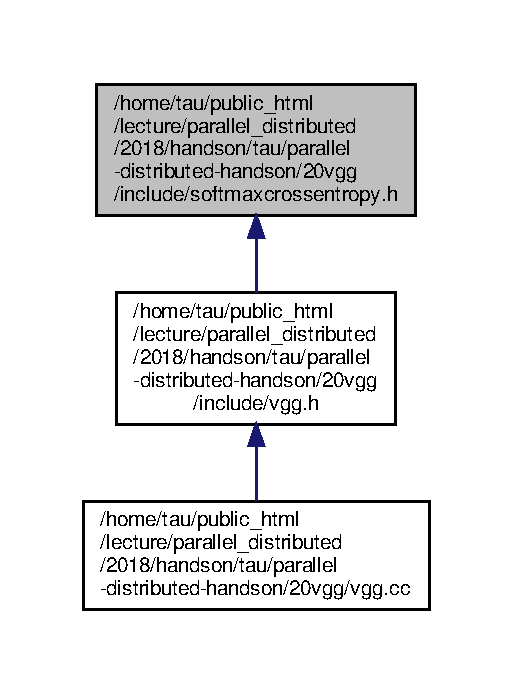
\includegraphics[width=246pt]{softmaxcrossentropy_8h__dep__incl}
\end{center}
\end{figure}
\subsection*{Classes}
\begin{DoxyCompactItemize}
\item 
struct \hyperlink{structSoftmaxCrossEntropy}{Softmax\+Cross\+Entropy$<$ max\+B, n\+C $>$}
\begin{DoxyCompactList}\small\item\em dropout layer \end{DoxyCompactList}\item 
struct \hyperlink{structSoftmaxCrossEntropy}{Softmax\+Cross\+Entropy$<$ max\+B, n\+C $>$}
\begin{DoxyCompactList}\small\item\em dropout layer \end{DoxyCompactList}\end{DoxyCompactItemize}
\subsection*{Functions}
\begin{DoxyCompactItemize}
\item 
{\footnotesize template$<$idx\+\_\+t maxB, idx\+\_\+t nC$>$ }\\\+\_\+\+\_\+global\+\_\+\+\_\+ void \hyperlink{softmaxcrossentropy_8h_a578aeeb166bd06e800d9b396eab48b35}{forward\+\_\+global} (\hyperlink{structSoftmaxCrossEntropy}{Softmax\+Cross\+Entropy}$<$ maxB, nC $>$ $\ast$dev, \hyperlink{structarray4}{array4}$<$ maxB, nC, 1, 1 $>$ $\ast$x\+\_\+dev, \hyperlink{structivec}{ivec}$<$ maxB $>$ $\ast$t\+\_\+dev)
\begin{DoxyCompactList}\small\item\em a global C\+U\+DA function that implements the baseline forward function for G\+PU \end{DoxyCompactList}\item 
{\footnotesize template$<$idx\+\_\+t maxB, idx\+\_\+t nC$>$ }\\\+\_\+\+\_\+global\+\_\+\+\_\+ void \hyperlink{softmaxcrossentropy_8h_a47d56a9a23e08247b227f4aac17413e0}{backward\+\_\+global} (\hyperlink{structSoftmaxCrossEntropy}{Softmax\+Cross\+Entropy}$<$ maxB, nC $>$ $\ast$dev, \hyperlink{structvec}{vec}$<$ maxB $>$ $\ast$gy\+\_\+dev)
\begin{DoxyCompactList}\small\item\em a global C\+U\+DA function that implements the baseline backward function for G\+PU \end{DoxyCompactList}\item 
{\footnotesize template$<$idx\+\_\+t maxB, idx\+\_\+t nC$>$ }\\static \hyperlink{vgg__util_8h_a1082d08aaa761215ec83e7149f27ad16}{real} \hyperlink{softmaxcrossentropy_8h_a650182ed5a860964171b71bf27aadb3f}{softmaxcrossentropy\+\_\+grad\+\_\+check\+\_\+rand} (\hyperlink{structcmdline__opt}{cmdline\+\_\+opt} opt, \hyperlink{structlogger}{logger} $\ast$lgr, \hyperlink{structrnd__gen__t}{rnd\+\_\+gen\+\_\+t} \&rg, \hyperlink{vgg__util_8h_a8e93478a00e685bea5e6a3f617bf03a3}{idx\+\_\+t} B)
\begin{DoxyCompactList}\small\item\em check the gradient computation of a softmaxcrossentropy layer \end{DoxyCompactList}\item 
int \hyperlink{softmaxcrossentropy_8h_ac16bb9a8e35d22b25f3e78e00b5d5231}{softmaxcrossentropy\+\_\+main} (int argc, char $\ast$$\ast$argv)
\begin{DoxyCompactList}\small\item\em entry point of this header file \end{DoxyCompactList}\end{DoxyCompactItemize}


\subsection{Detailed Description}
softmax + cross entropy layer 



\subsection{Function Documentation}
\mbox{\Hypertarget{softmaxcrossentropy_8h_a47d56a9a23e08247b227f4aac17413e0}\label{softmaxcrossentropy_8h_a47d56a9a23e08247b227f4aac17413e0}} 
\index{softmaxcrossentropy.\+h@{softmaxcrossentropy.\+h}!backward\+\_\+global@{backward\+\_\+global}}
\index{backward\+\_\+global@{backward\+\_\+global}!softmaxcrossentropy.\+h@{softmaxcrossentropy.\+h}}
\subsubsection{\texorpdfstring{backward\+\_\+global()}{backward\_global()}}
{\footnotesize\ttfamily template$<$idx\+\_\+t maxB, idx\+\_\+t nC$>$ \\
\+\_\+\+\_\+global\+\_\+\+\_\+ void backward\+\_\+global (\begin{DoxyParamCaption}\item[{\hyperlink{structSoftmaxCrossEntropy}{Softmax\+Cross\+Entropy}$<$ maxB, nC $>$ $\ast$}]{dev,  }\item[{\hyperlink{structvec}{vec}$<$ maxB $>$ $\ast$}]{gy\+\_\+dev }\end{DoxyParamCaption})}



a global C\+U\+DA function that implements the baseline backward function for G\+PU 


\begin{DoxyParams}{Parameters}
{\em (dev)} & the address of the device shadow of the object \\
\hline
{\em (gy\+\_\+dev)} & the address of the device shadow of the input matrix \\
\hline
\end{DoxyParams}
\begin{DoxySeeAlso}{See also}
backward\+\_\+dev 

backward\+\_\+gpu 
\end{DoxySeeAlso}
\mbox{\Hypertarget{softmaxcrossentropy_8h_a578aeeb166bd06e800d9b396eab48b35}\label{softmaxcrossentropy_8h_a578aeeb166bd06e800d9b396eab48b35}} 
\index{softmaxcrossentropy.\+h@{softmaxcrossentropy.\+h}!forward\+\_\+global@{forward\+\_\+global}}
\index{forward\+\_\+global@{forward\+\_\+global}!softmaxcrossentropy.\+h@{softmaxcrossentropy.\+h}}
\subsubsection{\texorpdfstring{forward\+\_\+global()}{forward\_global()}}
{\footnotesize\ttfamily template$<$idx\+\_\+t maxB, idx\+\_\+t nC$>$ \\
\+\_\+\+\_\+global\+\_\+\+\_\+ void forward\+\_\+global (\begin{DoxyParamCaption}\item[{\hyperlink{structSoftmaxCrossEntropy}{Softmax\+Cross\+Entropy}$<$ maxB, nC $>$ $\ast$}]{dev,  }\item[{\hyperlink{structarray4}{array4}$<$ maxB, nC, 1, 1 $>$ $\ast$}]{x\+\_\+dev,  }\item[{\hyperlink{structivec}{ivec}$<$ maxB $>$ $\ast$}]{t\+\_\+dev }\end{DoxyParamCaption})}



a global C\+U\+DA function that implements the baseline forward function for G\+PU 


\begin{DoxyParams}{Parameters}
{\em (dev)} & the address of the device shadow of the object \\
\hline
{\em (x\+\_\+dev)} & the address of the device shadow of the input matrix \\
\hline
{\em (t\+\_\+dev)} & the address of the device shadow of the true labels \\
\hline
\end{DoxyParams}
\begin{DoxySeeAlso}{See also}
forward\+\_\+dev 

forward\+\_\+gpu 
\end{DoxySeeAlso}
\mbox{\Hypertarget{softmaxcrossentropy_8h_a650182ed5a860964171b71bf27aadb3f}\label{softmaxcrossentropy_8h_a650182ed5a860964171b71bf27aadb3f}} 
\index{softmaxcrossentropy.\+h@{softmaxcrossentropy.\+h}!softmaxcrossentropy\+\_\+grad\+\_\+check\+\_\+rand@{softmaxcrossentropy\+\_\+grad\+\_\+check\+\_\+rand}}
\index{softmaxcrossentropy\+\_\+grad\+\_\+check\+\_\+rand@{softmaxcrossentropy\+\_\+grad\+\_\+check\+\_\+rand}!softmaxcrossentropy.\+h@{softmaxcrossentropy.\+h}}
\subsubsection{\texorpdfstring{softmaxcrossentropy\+\_\+grad\+\_\+check\+\_\+rand()}{softmaxcrossentropy\_grad\_check\_rand()}}
{\footnotesize\ttfamily template$<$idx\+\_\+t maxB, idx\+\_\+t nC$>$ \\
static \hyperlink{vgg__util_8h_a1082d08aaa761215ec83e7149f27ad16}{real} softmaxcrossentropy\+\_\+grad\+\_\+check\+\_\+rand (\begin{DoxyParamCaption}\item[{\hyperlink{structcmdline__opt}{cmdline\+\_\+opt}}]{opt,  }\item[{\hyperlink{structlogger}{logger} $\ast$}]{lgr,  }\item[{\hyperlink{structrnd__gen__t}{rnd\+\_\+gen\+\_\+t} \&}]{rg,  }\item[{\hyperlink{vgg__util_8h_a8e93478a00e685bea5e6a3f617bf03a3}{idx\+\_\+t}}]{B }\end{DoxyParamCaption})\hspace{0.3cm}{\ttfamily [static]}}



check the gradient computation of a softmaxcrossentropy layer 


\begin{DoxyParams}{Parameters}
{\em (opt)} & command line option \\
\hline
{\em (lgr)} & logger \\
\hline
{\em (rg)} & random number generator \\
\hline
{\em (\+B)} & the number of images \\
\hline
\end{DoxyParams}
\begin{DoxySeeAlso}{See also}
\hyperlink{softmaxcrossentropy_8h_ac16bb9a8e35d22b25f3e78e00b5d5231}{softmaxcrossentropy\+\_\+main}
\end{DoxySeeAlso}
it first makes a layer object with initial weights W and generates an input (x and t). it then creates two layers whose weights are slightly different from the original one by dw/2 (i.\+e., w-\/dw/2 and w+dw/2), as well as two inputs slighly different from the original inputs by dx/2 (x-\/dx/2 and x+dx/2). it then computes L(w,x), L(x-\/dw/2,x-\/dx/2) and L(w+dw/2,x+dw/2) and check if L(x+dw/2,x+dx/2)-\/L(x-\/dw/2,x-\/dx/2) is close to ∂\+L/∂x dx + ∂\+L/∂w dw. ∂\+L/∂x and ∂\+L/∂w are obtained by backward computation. This is essentially checking if the gradients obtained by backward computation correctly approximates the diff of the output. \mbox{\Hypertarget{softmaxcrossentropy_8h_ac16bb9a8e35d22b25f3e78e00b5d5231}\label{softmaxcrossentropy_8h_ac16bb9a8e35d22b25f3e78e00b5d5231}} 
\index{softmaxcrossentropy.\+h@{softmaxcrossentropy.\+h}!softmaxcrossentropy\+\_\+main@{softmaxcrossentropy\+\_\+main}}
\index{softmaxcrossentropy\+\_\+main@{softmaxcrossentropy\+\_\+main}!softmaxcrossentropy.\+h@{softmaxcrossentropy.\+h}}
\subsubsection{\texorpdfstring{softmaxcrossentropy\+\_\+main()}{softmaxcrossentropy\_main()}}
{\footnotesize\ttfamily int softmaxcrossentropy\+\_\+main (\begin{DoxyParamCaption}\item[{int}]{argc,  }\item[{char $\ast$$\ast$}]{argv }\end{DoxyParamCaption})}



entry point of this header file 


\begin{DoxyParams}{Parameters}
{\em (argc)} & the number of command line args \\
\hline
{\em (argv)} & command line args \\
\hline
\end{DoxyParams}
\begin{DoxySeeAlso}{See also}
\hyperlink{softmaxcrossentropy_8h_a650182ed5a860964171b71bf27aadb3f}{softmaxcrossentropy\+\_\+grad\+\_\+check\+\_\+rand}
\end{DoxySeeAlso}
if this header file is included from a main C++ file and define softmaxcrossentropy\+\_\+main to be main (e.\+g., with -\/\+Dsoftmaxcrossentropy\+\_\+main=main), then this function becomes th main function of the executable. it calls softmaxcrossentropy\+\_\+grad\+\_\+check\+\_\+rand repeatedly to test the implementation of \hyperlink{structVGG}{V\+GG} network. 
\hypertarget{vgg_8h}{}\section{/home/tau/public\+\_\+html/lecture/parallel\+\_\+distributed/2018/handson/tau/parallel-\/distributed-\/handson/20vgg/include/vgg.h File Reference}
\label{vgg_8h}\index{/home/tau/public\+\_\+html/lecture/parallel\+\_\+distributed/2018/handson/tau/parallel-\/distributed-\/handson/20vgg/include/vgg.\+h@{/home/tau/public\+\_\+html/lecture/parallel\+\_\+distributed/2018/handson/tau/parallel-\/distributed-\/handson/20vgg/include/vgg.\+h}}


\hyperlink{structVGG}{V\+GG} network.  


{\ttfamily \#include \char`\"{}vgg\+\_\+util.\+h\char`\"{}}\newline
{\ttfamily \#include \char`\"{}vgg\+\_\+arrays.\+h\char`\"{}}\newline
{\ttfamily \#include \char`\"{}block.\+h\char`\"{}}\newline
{\ttfamily \#include \char`\"{}linear.\+h\char`\"{}}\newline
{\ttfamily \#include \char`\"{}dropout.\+h\char`\"{}}\newline
{\ttfamily \#include \char`\"{}maxpooling.\+h\char`\"{}}\newline
{\ttfamily \#include \char`\"{}softmaxcrossentropy.\+h\char`\"{}}\newline
Include dependency graph for vgg.\+h\+:\nopagebreak
\begin{figure}[H]
\begin{center}
\leavevmode
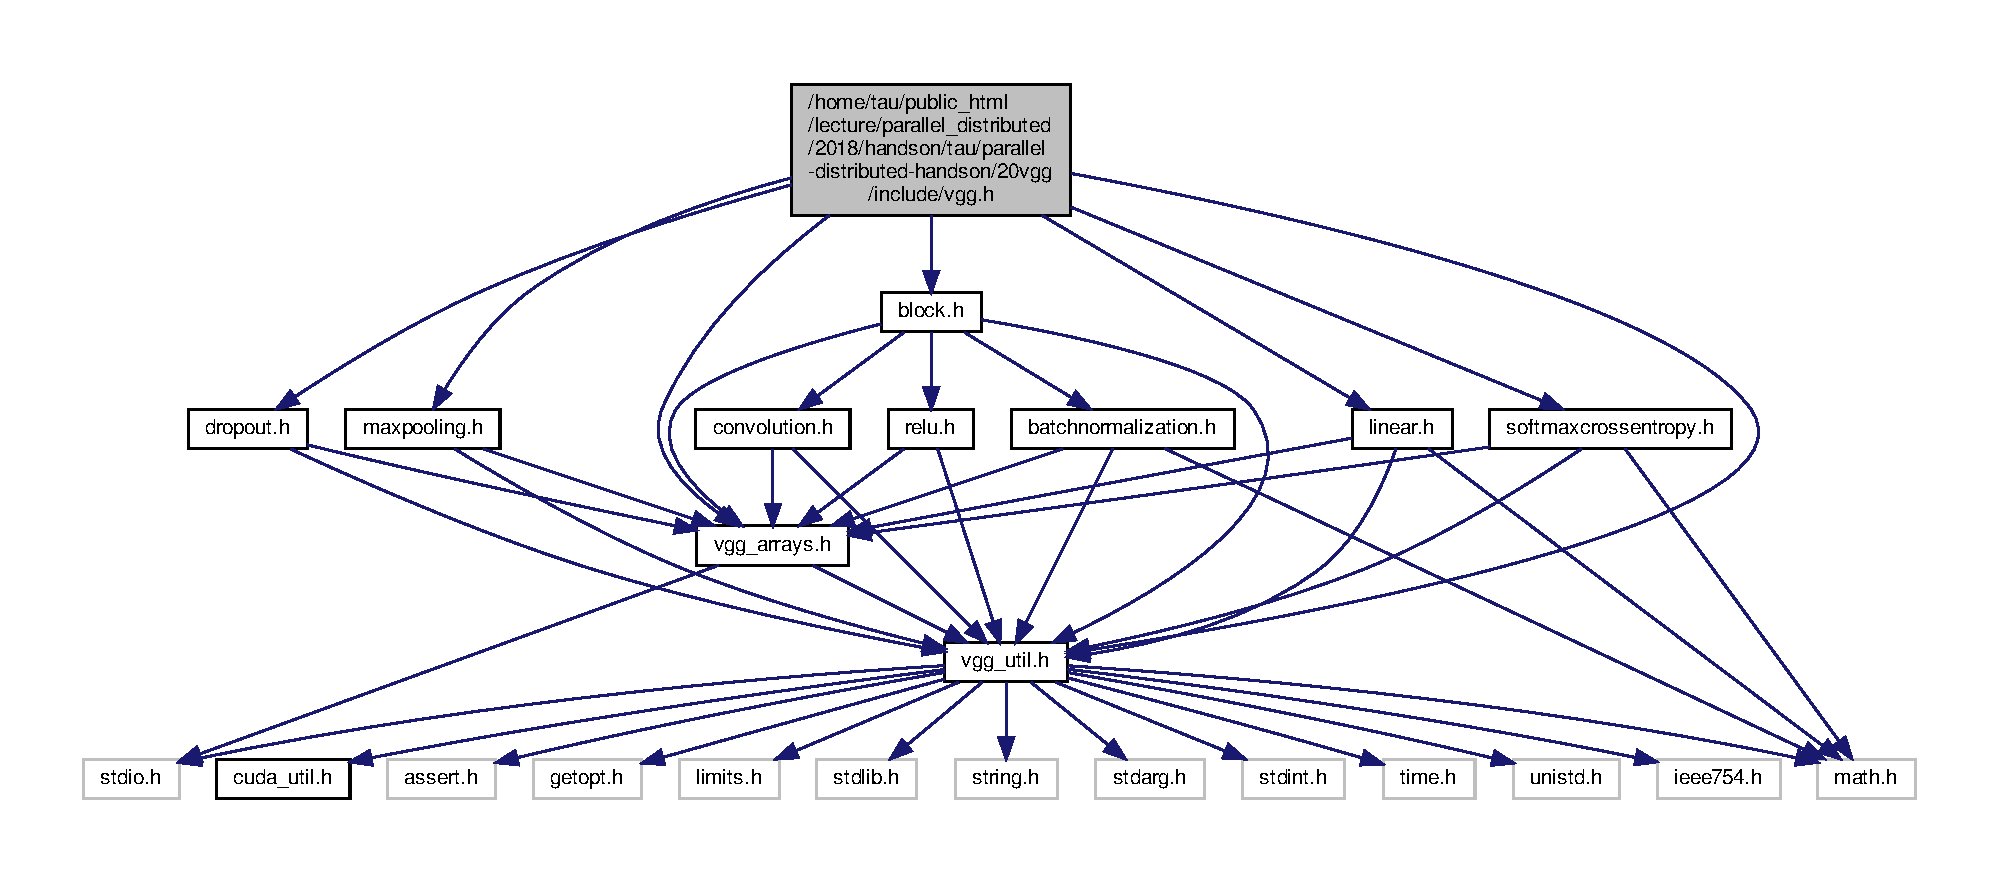
\includegraphics[width=350pt]{vgg_8h__incl}
\end{center}
\end{figure}
This graph shows which files directly or indirectly include this file\+:\nopagebreak
\begin{figure}[H]
\begin{center}
\leavevmode
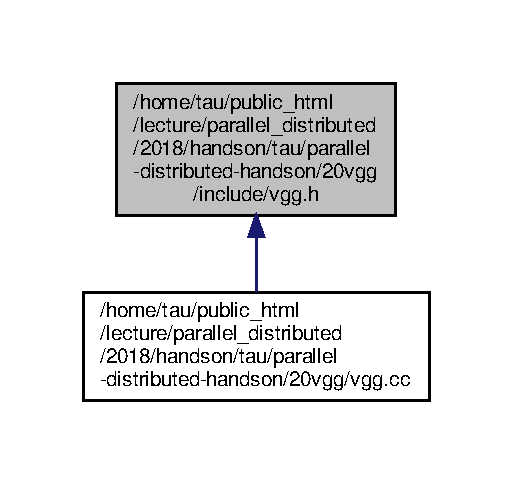
\includegraphics[width=246pt]{vgg_8h__dep__incl}
\end{center}
\end{figure}
\subsection*{Classes}
\begin{DoxyCompactItemize}
\item 
struct \hyperlink{structVGG}{V\+G\+G$<$ max\+B, C0, H, W, K, S, C1, n\+C $>$}
\begin{DoxyCompactList}\small\item\em \hyperlink{structVGG}{V\+GG} network. \end{DoxyCompactList}\end{DoxyCompactItemize}
\subsection*{Functions}
\begin{DoxyCompactItemize}
\item 
{\footnotesize template$<$idx\+\_\+t maxB, idx\+\_\+t C0, idx\+\_\+t H, idx\+\_\+t W, idx\+\_\+t K, idx\+\_\+t S, idx\+\_\+t C1, idx\+\_\+t nC$>$ }\\static \hyperlink{vgg__util_8h_a1082d08aaa761215ec83e7149f27ad16}{real} \hyperlink{vgg_8h_a2926d1b596f84303d320c748d27a9638}{vgg\+\_\+grad\+\_\+check\+\_\+rand} (\hyperlink{structcmdline__opt}{cmdline\+\_\+opt} opt, \hyperlink{structlogger}{logger} $\ast$lgr, \hyperlink{structrnd__gen__t}{rnd\+\_\+gen\+\_\+t} \&rg, \hyperlink{vgg__util_8h_a8e93478a00e685bea5e6a3f617bf03a3}{idx\+\_\+t} B)
\begin{DoxyCompactList}\small\item\em check the gradient computation of a \hyperlink{structVGG}{V\+GG} network \end{DoxyCompactList}\item 
int \hyperlink{vgg_8h_ade99540bb2e3dddf1498e22a2d05ca9a}{vgg\+\_\+main} (int argc, char $\ast$$\ast$argv)
\begin{DoxyCompactList}\small\item\em entry point of this header file \end{DoxyCompactList}\end{DoxyCompactItemize}


\subsection{Detailed Description}
\hyperlink{structVGG}{V\+GG} network. 



\subsection{Function Documentation}
\mbox{\Hypertarget{vgg_8h_a2926d1b596f84303d320c748d27a9638}\label{vgg_8h_a2926d1b596f84303d320c748d27a9638}} 
\index{vgg.\+h@{vgg.\+h}!vgg\+\_\+grad\+\_\+check\+\_\+rand@{vgg\+\_\+grad\+\_\+check\+\_\+rand}}
\index{vgg\+\_\+grad\+\_\+check\+\_\+rand@{vgg\+\_\+grad\+\_\+check\+\_\+rand}!vgg.\+h@{vgg.\+h}}
\subsubsection{\texorpdfstring{vgg\+\_\+grad\+\_\+check\+\_\+rand()}{vgg\_grad\_check\_rand()}}
{\footnotesize\ttfamily template$<$idx\+\_\+t maxB, idx\+\_\+t C0, idx\+\_\+t H, idx\+\_\+t W, idx\+\_\+t K, idx\+\_\+t S, idx\+\_\+t C1, idx\+\_\+t nC$>$ \\
static \hyperlink{vgg__util_8h_a1082d08aaa761215ec83e7149f27ad16}{real} vgg\+\_\+grad\+\_\+check\+\_\+rand (\begin{DoxyParamCaption}\item[{\hyperlink{structcmdline__opt}{cmdline\+\_\+opt}}]{opt,  }\item[{\hyperlink{structlogger}{logger} $\ast$}]{lgr,  }\item[{\hyperlink{structrnd__gen__t}{rnd\+\_\+gen\+\_\+t} \&}]{rg,  }\item[{\hyperlink{vgg__util_8h_a8e93478a00e685bea5e6a3f617bf03a3}{idx\+\_\+t}}]{B }\end{DoxyParamCaption})\hspace{0.3cm}{\ttfamily [static]}}



check the gradient computation of a \hyperlink{structVGG}{V\+GG} network 


\begin{DoxyParams}{Parameters}
{\em (opt)} & command line option \\
\hline
{\em (lgr)} & logger \\
\hline
{\em (rg)} & random number generator \\
\hline
{\em (\+B)} & the number of images \\
\hline
\end{DoxyParams}
\begin{DoxySeeAlso}{See also}
\hyperlink{vgg_8h_ade99540bb2e3dddf1498e22a2d05ca9a}{vgg\+\_\+main}
\end{DoxySeeAlso}
it first makes a \hyperlink{structVGG}{V\+GG} network with initial weights W and generates an input (x and t). it then creates two \hyperlink{structVGG}{V\+GG} networks whose weights are slightly different from the original one by dw/2 (i.\+e., w-\/dw/2 and w+dw/2), as well as two inputs slighly different from the original inputs by dx/2 (x-\/dx/2 and x+dx/2). it then computes L(w,x), L(x-\/dw/2,x-\/dx/2) and L(w+dw/2,x+dw/2) and check if L(x+dw/2,x+dx/2)-\/L(x-\/dw/2,x-\/dx/2) is close to ∂\+L/∂x dx + ∂\+L/∂w dw. ∂\+L/∂x and ∂\+L/∂w are obtained by backward computation. This is essentially checking if the gradients obtained by backward computation correctly approximates the diff of the output. \mbox{\Hypertarget{vgg_8h_ade99540bb2e3dddf1498e22a2d05ca9a}\label{vgg_8h_ade99540bb2e3dddf1498e22a2d05ca9a}} 
\index{vgg.\+h@{vgg.\+h}!vgg\+\_\+main@{vgg\+\_\+main}}
\index{vgg\+\_\+main@{vgg\+\_\+main}!vgg.\+h@{vgg.\+h}}
\subsubsection{\texorpdfstring{vgg\+\_\+main()}{vgg\_main()}}
{\footnotesize\ttfamily int vgg\+\_\+main (\begin{DoxyParamCaption}\item[{int}]{argc,  }\item[{char $\ast$$\ast$}]{argv }\end{DoxyParamCaption})}



entry point of this header file 


\begin{DoxyParams}{Parameters}
{\em (argc)} & the number of command line args \\
\hline
{\em (argv)} & command line args \\
\hline
\end{DoxyParams}
\begin{DoxySeeAlso}{See also}
\hyperlink{vgg_8h_a2926d1b596f84303d320c748d27a9638}{vgg\+\_\+grad\+\_\+check\+\_\+rand}
\end{DoxySeeAlso}
if this header file is included from a main C++ file and define vgg\+\_\+main to be main (e.\+g., with -\/\+Dvgg\+\_\+main=main), then this function becomes th main function of the executable. it calls vgg\+\_\+grad\+\_\+check\+\_\+rand repeatedly to test the implementation of \hyperlink{structVGG}{V\+GG} network. 
\hypertarget{vgg__arrays_8h}{}\section{/home/tau/public\+\_\+html/lecture/parallel\+\_\+distributed/2018/handson/tau/parallel-\/distributed-\/handson/20vgg/include/vgg\+\_\+arrays.h File Reference}
\label{vgg__arrays_8h}\index{/home/tau/public\+\_\+html/lecture/parallel\+\_\+distributed/2018/handson/tau/parallel-\/distributed-\/handson/20vgg/include/vgg\+\_\+arrays.\+h@{/home/tau/public\+\_\+html/lecture/parallel\+\_\+distributed/2018/handson/tau/parallel-\/distributed-\/handson/20vgg/include/vgg\+\_\+arrays.\+h}}


vectors, matrices, and multi-\/dimensional arrays  


{\ttfamily \#include $<$stdio.\+h$>$}\newline
{\ttfamily \#include \char`\"{}vgg\+\_\+util.\+h\char`\"{}}\newline
Include dependency graph for vgg\+\_\+arrays.\+h\+:
\nopagebreak
\begin{figure}[H]
\begin{center}
\leavevmode
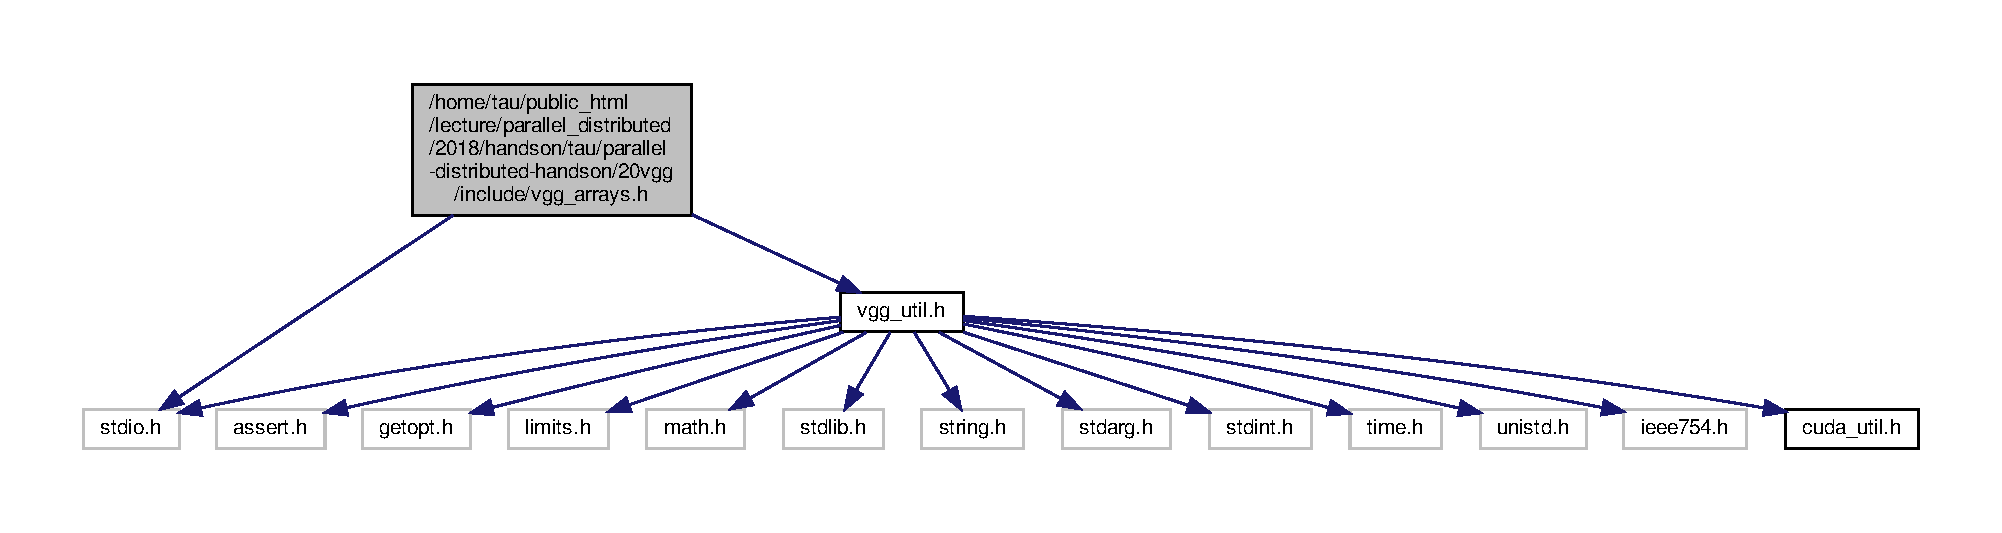
\includegraphics[width=350pt]{vgg__arrays_8h__incl}
\end{center}
\end{figure}
This graph shows which files directly or indirectly include this file\+:
\nopagebreak
\begin{figure}[H]
\begin{center}
\leavevmode
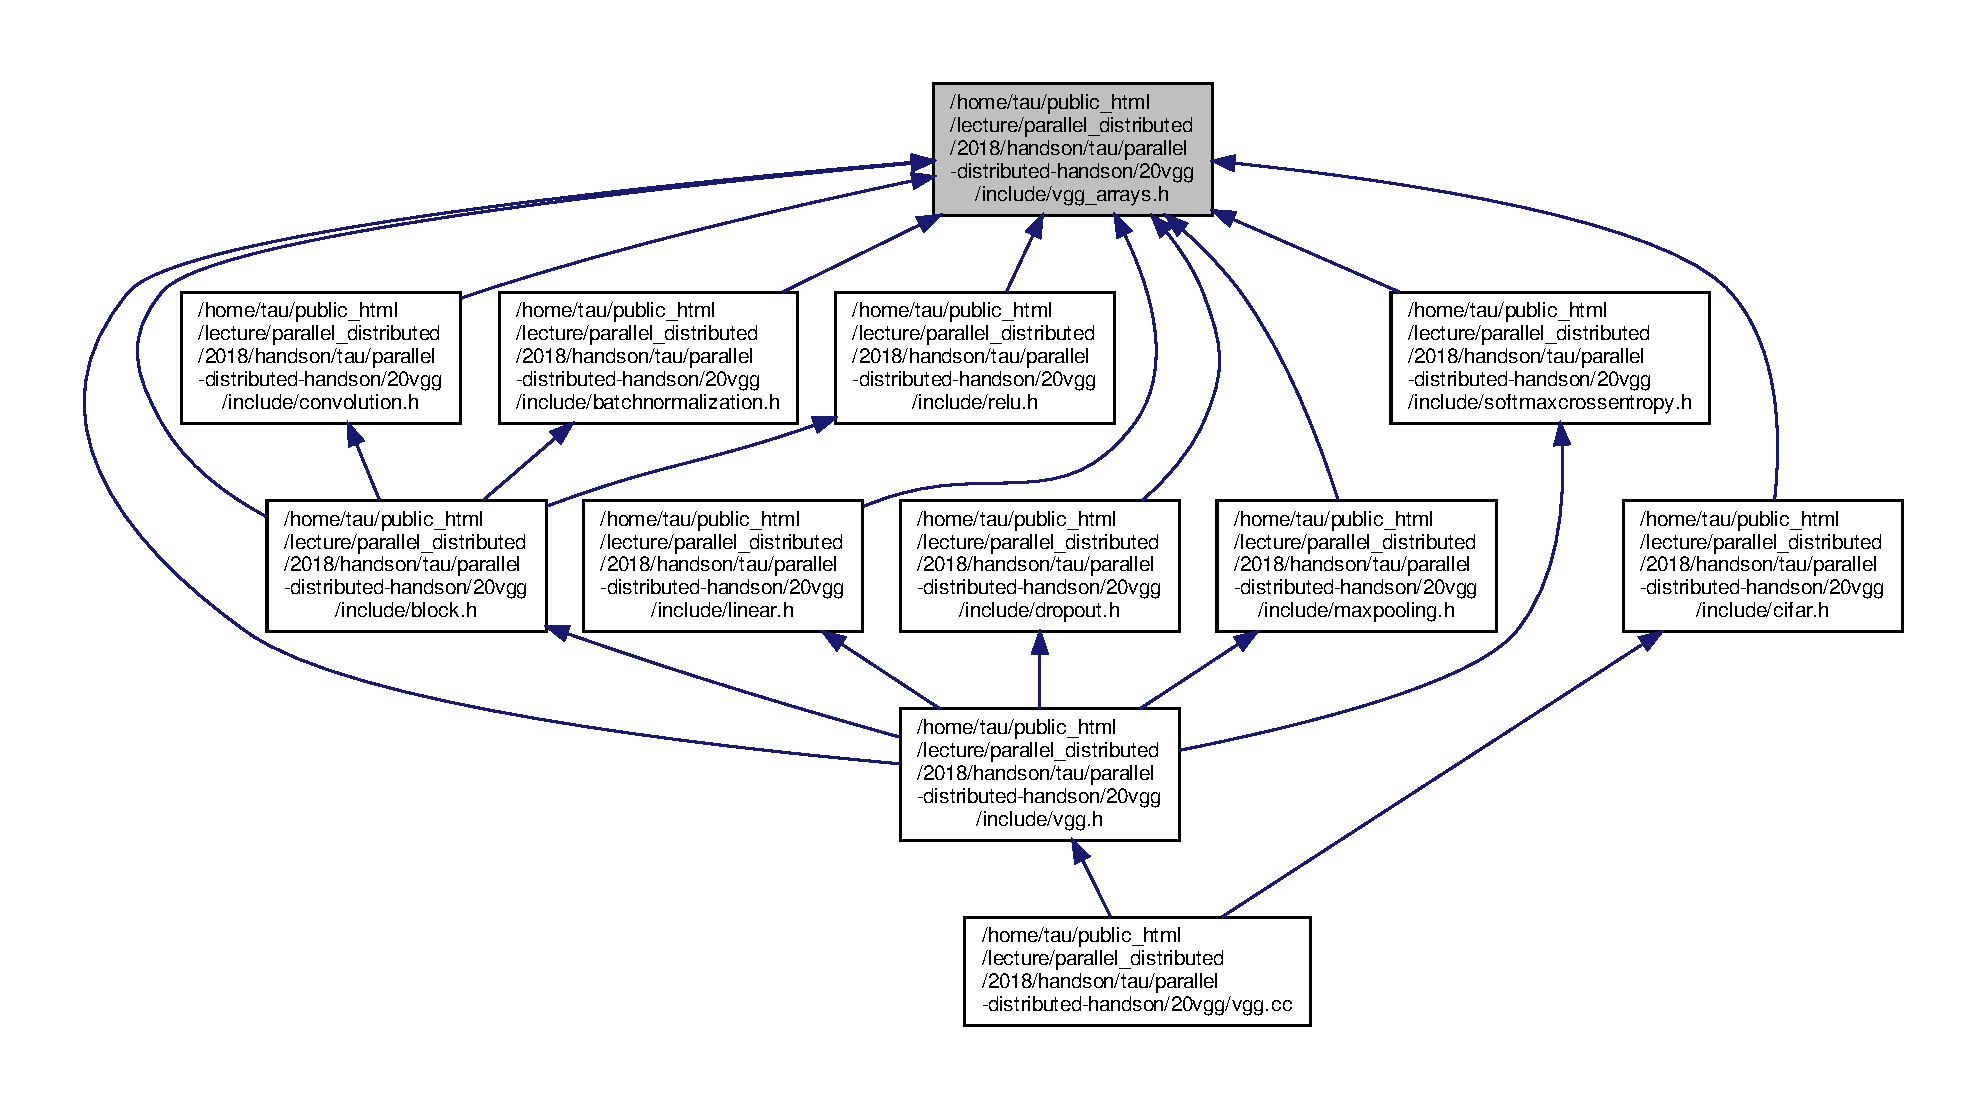
\includegraphics[width=350pt]{vgg__arrays_8h__dep__incl}
\end{center}
\end{figure}
\subsection*{Classes}
\begin{DoxyCompactItemize}
\item 
struct \hyperlink{structvec}{vec$<$ N $>$}
\begin{DoxyCompactList}\small\item\em vector \end{DoxyCompactList}\item 
struct \hyperlink{structivec}{ivec$<$ N $>$}
\begin{DoxyCompactList}\small\item\em integer vector \end{DoxyCompactList}\item 
struct \hyperlink{structarray2}{array2$<$ M, N $>$}
\begin{DoxyCompactList}\small\item\em matrix (2D array) \end{DoxyCompactList}\item 
struct \hyperlink{structarray4}{array4$<$ max\+B, C, H, W $>$}
\begin{DoxyCompactList}\small\item\em 4D array \end{DoxyCompactList}\item 
struct \hyperlink{structwarray4}{warray4$<$ O\+C, I\+C, H, W $>$}
\begin{DoxyCompactList}\small\item\em 4D array for convolution \end{DoxyCompactList}\end{DoxyCompactItemize}
\subsection*{Macros}
\begin{DoxyCompactItemize}
\item 
\mbox{\Hypertarget{vgg__arrays_8h_ab238ad0298ba0f760c1cc1afa64ab86d}\label{vgg__arrays_8h_ab238ad0298ba0f760c1cc1afa64ab86d}} 
\#define \hyperlink{vgg__arrays_8h_ab238ad0298ba0f760c1cc1afa64ab86d}{range\+\_\+chk}(a,  x,  b)
\begin{DoxyCompactList}\small\item\em array bounds check. turn off (on) if -\/\+D\+A\+R\+R\+A\+Y\+\_\+\+I\+N\+D\+E\+X\+\_\+\+C\+H\+E\+CK=0 (1) is given. turn it on when you are debugging your code. turn it off when you are measuring the performance. \end{DoxyCompactList}\end{DoxyCompactItemize}
\subsection*{Functions}
\begin{DoxyCompactItemize}
\item 
\+\_\+\+\_\+device\+\_\+\+\_\+ static \+\_\+\+\_\+host\+\_\+\+\_\+ void \hyperlink{vgg__arrays_8h_a8e9c898312e7fc15a07310b1a55284eb}{range\+\_\+chk\+\_\+} (\hyperlink{vgg__util_8h_a8e93478a00e685bea5e6a3f617bf03a3}{idx\+\_\+t} a, \hyperlink{vgg__util_8h_a8e93478a00e685bea5e6a3f617bf03a3}{idx\+\_\+t} x, \hyperlink{vgg__util_8h_a8e93478a00e685bea5e6a3f617bf03a3}{idx\+\_\+t} b, const char $\ast$a\+\_\+str, const char $\ast$x\+\_\+str, const char $\ast$b\+\_\+str, const char $\ast$file, int line)
\begin{DoxyCompactList}\small\item\em aux function for array bounds checking \end{DoxyCompactList}\item 
\mbox{\Hypertarget{vgg__arrays_8h_a319f9d8c1f71686c088abf70f7e24d1e}\label{vgg__arrays_8h_a319f9d8c1f71686c088abf70f7e24d1e}} 
int \hyperlink{vgg__arrays_8h_a319f9d8c1f71686c088abf70f7e24d1e}{vgg\+\_\+arrays\+\_\+main} (int argc, char $\ast$$\ast$argv)
\begin{DoxyCompactList}\small\item\em entry point \end{DoxyCompactList}\item 
\mbox{\Hypertarget{vgg__arrays_8h_a177ed30da9fa6624ec7f35ed35454a76}\label{vgg__arrays_8h_a177ed30da9fa6624ec7f35ed35454a76}} 
void \hyperlink{vgg__arrays_8h_a177ed30da9fa6624ec7f35ed35454a76}{vgg\+\_\+arrays\+\_\+use\+\_\+unused\+\_\+functions} ()
\begin{DoxyCompactList}\small\item\em suppress unused function warning \end{DoxyCompactList}\end{DoxyCompactItemize}


\subsection{Detailed Description}
vectors, matrices, and multi-\/dimensional arrays 



\subsection{Function Documentation}
\mbox{\Hypertarget{vgg__arrays_8h_a8e9c898312e7fc15a07310b1a55284eb}\label{vgg__arrays_8h_a8e9c898312e7fc15a07310b1a55284eb}} 
\index{vgg\+\_\+arrays.\+h@{vgg\+\_\+arrays.\+h}!range\+\_\+chk\+\_\+@{range\+\_\+chk\+\_\+}}
\index{range\+\_\+chk\+\_\+@{range\+\_\+chk\+\_\+}!vgg\+\_\+arrays.\+h@{vgg\+\_\+arrays.\+h}}
\subsubsection{\texorpdfstring{range\+\_\+chk\+\_\+()}{range\_chk\_()}}
{\footnotesize\ttfamily \+\_\+\+\_\+device\+\_\+\+\_\+ static \+\_\+\+\_\+host\+\_\+\+\_\+ void range\+\_\+chk\+\_\+ (\begin{DoxyParamCaption}\item[{\hyperlink{vgg__util_8h_a8e93478a00e685bea5e6a3f617bf03a3}{idx\+\_\+t}}]{a,  }\item[{\hyperlink{vgg__util_8h_a8e93478a00e685bea5e6a3f617bf03a3}{idx\+\_\+t}}]{x,  }\item[{\hyperlink{vgg__util_8h_a8e93478a00e685bea5e6a3f617bf03a3}{idx\+\_\+t}}]{b,  }\item[{const char $\ast$}]{a\+\_\+str,  }\item[{const char $\ast$}]{x\+\_\+str,  }\item[{const char $\ast$}]{b\+\_\+str,  }\item[{const char $\ast$}]{file,  }\item[{int}]{line }\end{DoxyParamCaption})\hspace{0.3cm}{\ttfamily [static]}}



aux function for array bounds checking 


\begin{DoxyParams}{Parameters}
{\em (a)} & the lower bound \\
\hline
{\em (x)} & the index \\
\hline
{\em (b)} & the upper bound + 1 \\
\hline
{\em (a\+\_\+str)} & the string representation of a \\
\hline
{\em (x\+\_\+str)} & the string representation of x \\
\hline
{\em (b\+\_\+str)} & the string representation of b \\
\hline
{\em (file)} & the file name from which it gets called \\
\hline
{\em (line)} & the line number from which it gets called\\
\hline
\end{DoxyParams}
it checks if a$<$=x$<$b holds. if not, it shows an error message. on cpu, the error message contains the location where the error happened. 
\hypertarget{vgg__util_8h}{}\section{/home/tau/public\+\_\+html/lecture/parallel\+\_\+distributed/2018/handson/tau/parallel-\/distributed-\/handson/20vgg/include/vgg\+\_\+util.h File Reference}
\label{vgg__util_8h}\index{/home/tau/public\+\_\+html/lecture/parallel\+\_\+distributed/2018/handson/tau/parallel-\/distributed-\/handson/20vgg/include/vgg\+\_\+util.\+h@{/home/tau/public\+\_\+html/lecture/parallel\+\_\+distributed/2018/handson/tau/parallel-\/distributed-\/handson/20vgg/include/vgg\+\_\+util.\+h}}


\hyperlink{structVGG}{V\+GG} utility functions/classes.  


{\ttfamily \#include $<$assert.\+h$>$}\newline
{\ttfamily \#include $<$getopt.\+h$>$}\newline
{\ttfamily \#include $<$limits.\+h$>$}\newline
{\ttfamily \#include $<$math.\+h$>$}\newline
{\ttfamily \#include $<$stdio.\+h$>$}\newline
{\ttfamily \#include $<$stdlib.\+h$>$}\newline
{\ttfamily \#include $<$string.\+h$>$}\newline
{\ttfamily \#include $<$stdarg.\+h$>$}\newline
{\ttfamily \#include $<$stdint.\+h$>$}\newline
{\ttfamily \#include $<$time.\+h$>$}\newline
{\ttfamily \#include $<$unistd.\+h$>$}\newline
{\ttfamily \#include $<$ieee754.\+h$>$}\newline
{\ttfamily \#include \char`\"{}cuda\+\_\+util.\+h\char`\"{}}\newline
Include dependency graph for vgg\+\_\+util.\+h\+:\nopagebreak
\begin{figure}[H]
\begin{center}
\leavevmode
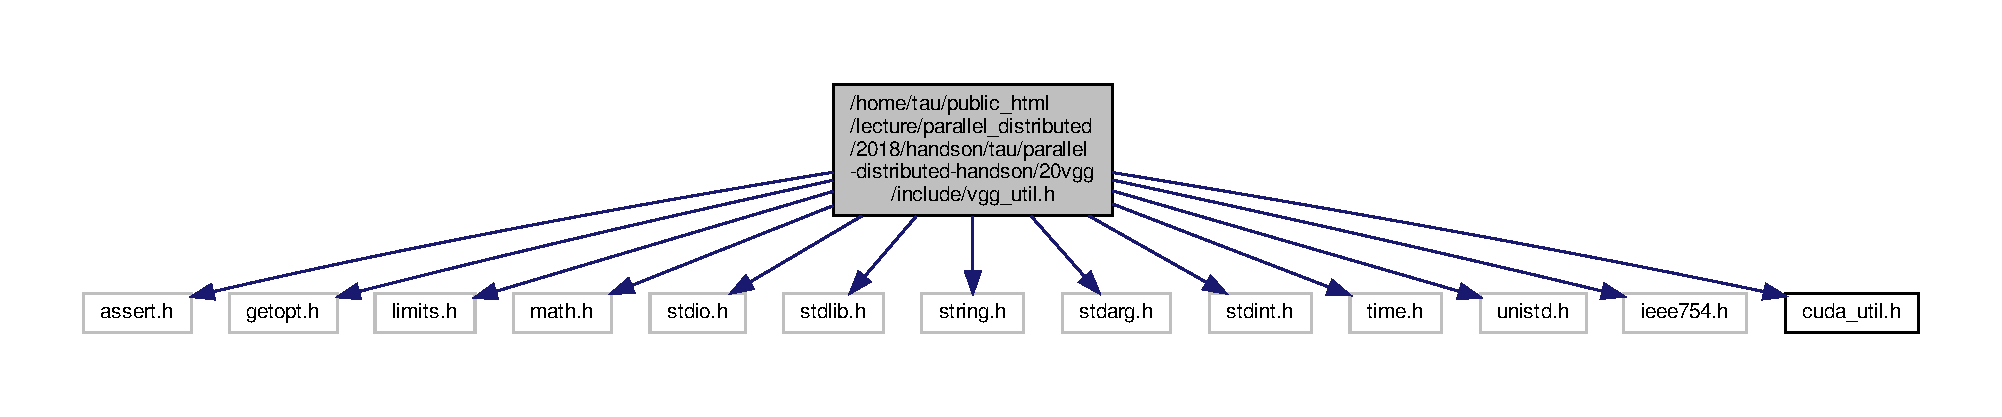
\includegraphics[width=350pt]{vgg__util_8h__incl}
\end{center}
\end{figure}
This graph shows which files directly or indirectly include this file\+:\nopagebreak
\begin{figure}[H]
\begin{center}
\leavevmode
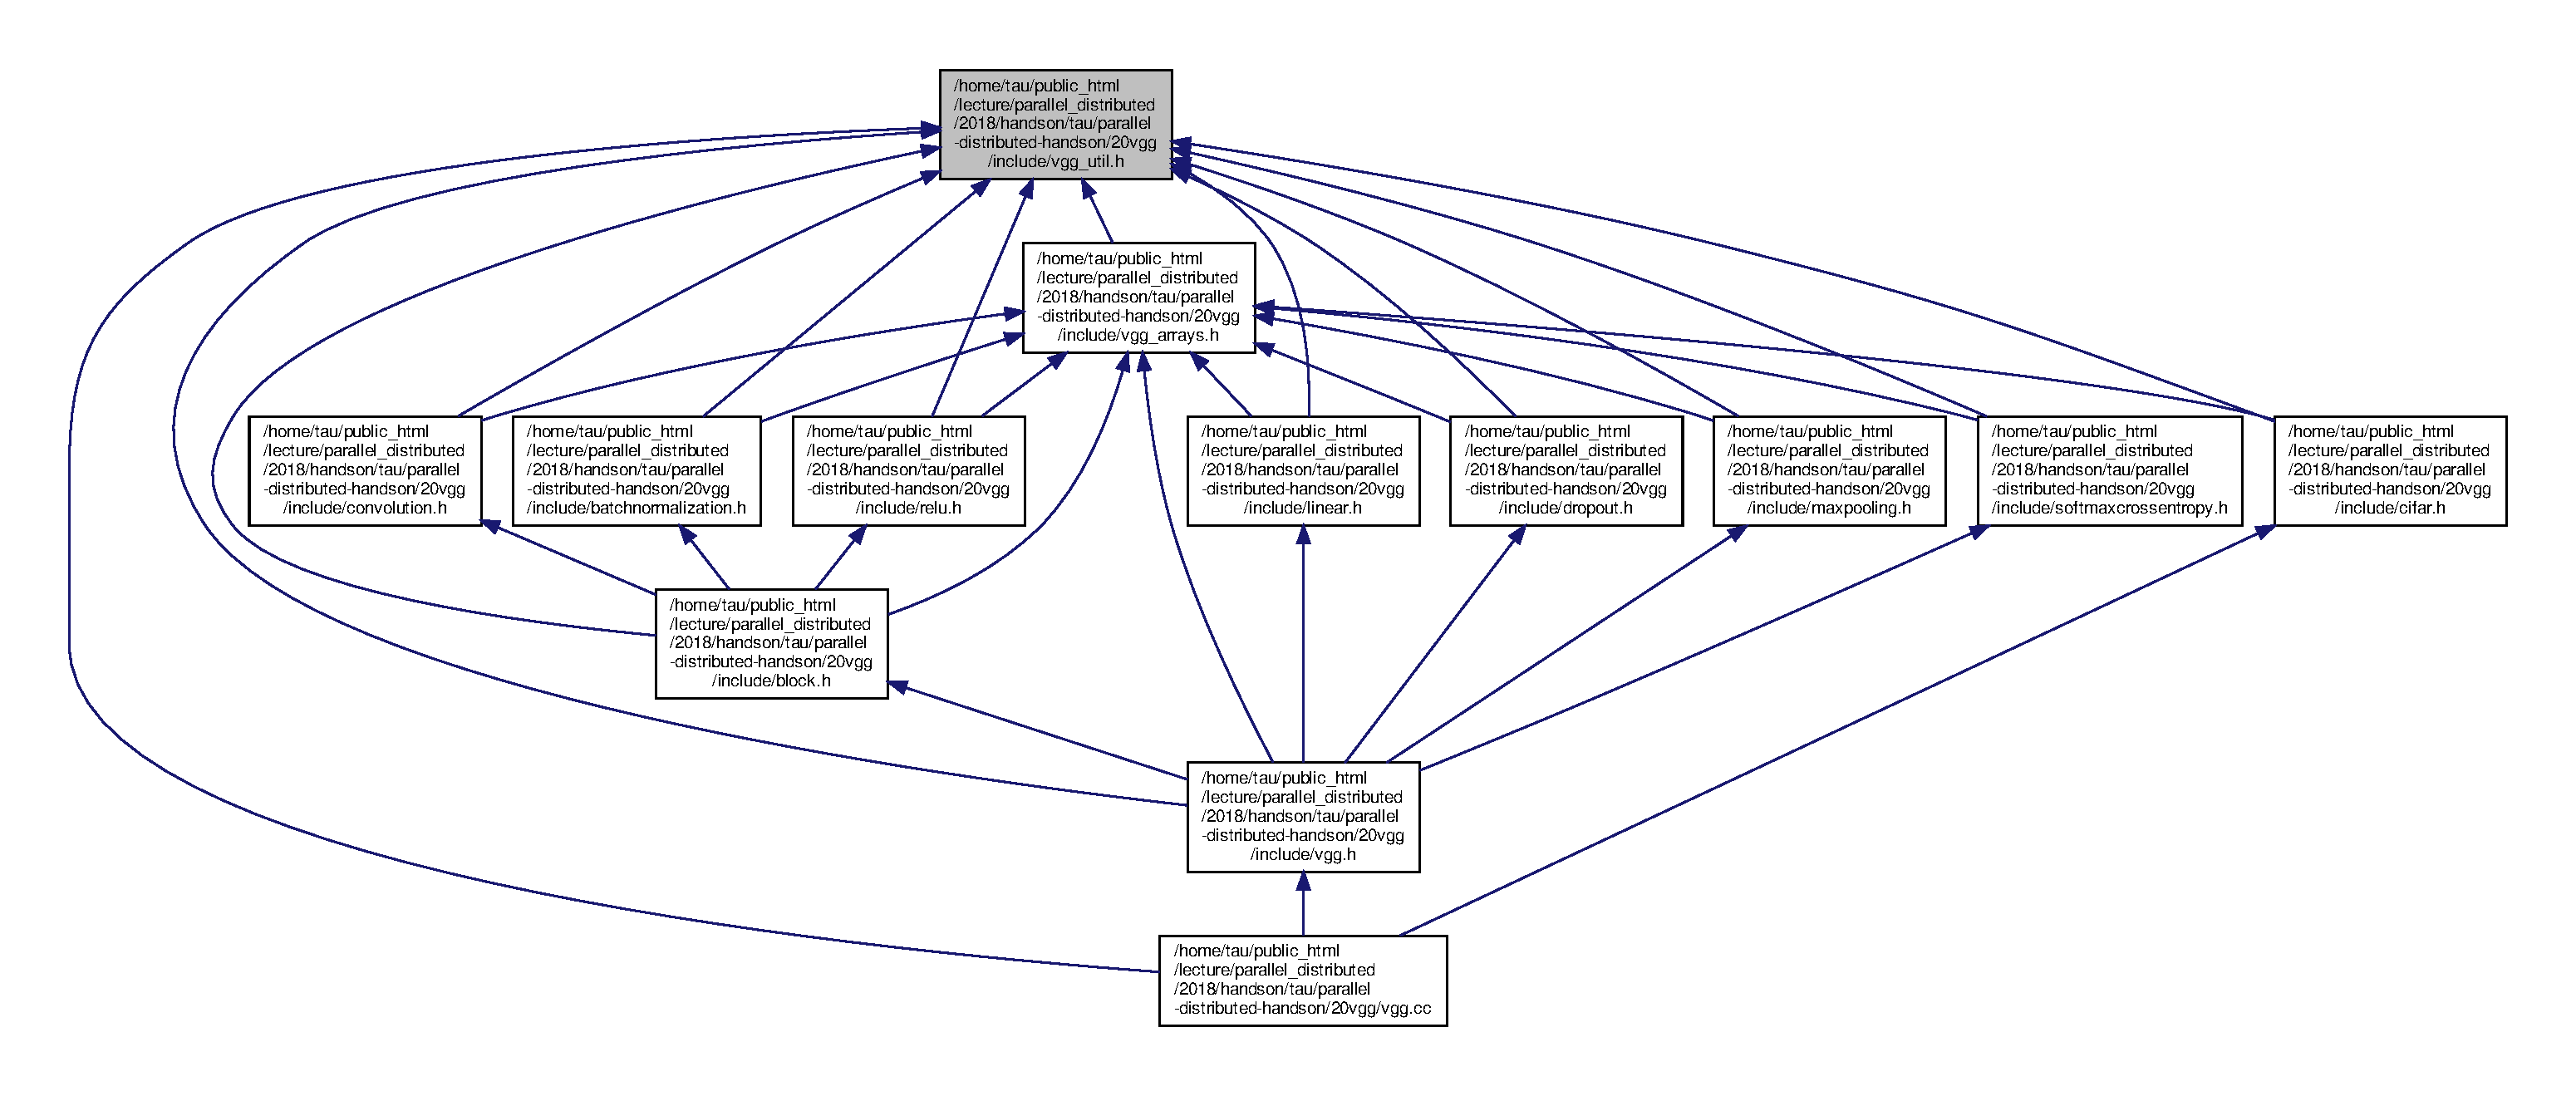
\includegraphics[width=350pt]{vgg__util_8h__dep__incl}
\end{center}
\end{figure}
\subsection*{Classes}
\begin{DoxyCompactItemize}
\item 
struct \hyperlink{structcmdline__opt}{cmdline\+\_\+opt}
\begin{DoxyCompactList}\small\item\em command line options \end{DoxyCompactList}\item 
struct \hyperlink{structtsc__t}{tsc\+\_\+t}
\begin{DoxyCompactList}\small\item\em timestamp \end{DoxyCompactList}\item 
struct \hyperlink{structrnd__gen__t}{rnd\+\_\+gen\+\_\+t}
\begin{DoxyCompactList}\small\item\em pseudo random number generator crafted from man erand48 + libc source \end{DoxyCompactList}\item 
struct \hyperlink{structlogger}{logger}
\begin{DoxyCompactList}\small\item\em logging object \end{DoxyCompactList}\end{DoxyCompactItemize}
\subsection*{Macros}
\begin{DoxyCompactItemize}
\item 
\mbox{\Hypertarget{vgg__util_8h_a731a48e08c9b18c801b19dba5392ebd3}\label{vgg__util_8h_a731a48e08c9b18c801b19dba5392ebd3}} 
\#define \hyperlink{vgg__util_8h_a731a48e08c9b18c801b19dba5392ebd3}{real\+\_\+type}~float
\begin{DoxyCompactList}\small\item\em real\+\_\+type is float if not supplied \end{DoxyCompactList}\item 
\mbox{\Hypertarget{vgg__util_8h_a5451ba9b35b36fff317b514218f7fcb8}\label{vgg__util_8h_a5451ba9b35b36fff317b514218f7fcb8}} 
\#define \hyperlink{vgg__util_8h_a5451ba9b35b36fff317b514218f7fcb8}{err\+\_\+gpu\+\_\+algo\+\_\+no\+\_\+gpu}(algo\+\_\+s)~\hyperlink{vgg__util_8h_abbf3f6741f183610f693696b84c6db8c}{err\+\_\+gpu\+\_\+algo\+\_\+no\+\_\+gpu\+\_\+}(\+\_\+\+\_\+\+F\+I\+L\+E\+\_\+\+\_\+, \+\_\+\+\_\+\+L\+I\+N\+E\+\_\+\+\_\+, algo\+\_\+s)
\begin{DoxyCompactList}\small\item\em signal a fatal error when a gpu algorithm gets called for cpu only compilation \end{DoxyCompactList}\item 
\#define \hyperlink{vgg__util_8h_a3729b3313855ba6b5af5e17b237c3558}{log\+\_\+start\+\_\+fun}(lgr)~lgr-\/$>$log\+\_\+start\+\_\+fun\+\_\+(\+\_\+\+\_\+\+P\+R\+E\+T\+T\+Y\+\_\+\+F\+U\+N\+C\+T\+I\+O\+N\+\_\+\+\_\+)
\begin{DoxyCompactList}\small\item\em log the start of the current function \end{DoxyCompactList}\item 
\#define \hyperlink{vgg__util_8h_ac27fe6f3d72940b92349035afd50ec6f}{log\+\_\+end\+\_\+fun}(lgr,  t0,  t1)~lgr-\/$>$log\+\_\+end\+\_\+fun\+\_\+(\+\_\+\+\_\+\+P\+R\+E\+T\+T\+Y\+\_\+\+F\+U\+N\+C\+T\+I\+O\+N\+\_\+\+\_\+, t0, t1)
\begin{DoxyCompactList}\small\item\em log the end of the current function \end{DoxyCompactList}\end{DoxyCompactItemize}
\subsection*{Typedefs}
\begin{DoxyCompactItemize}
\item 
\mbox{\Hypertarget{vgg__util_8h_a8e93478a00e685bea5e6a3f617bf03a3}\label{vgg__util_8h_a8e93478a00e685bea5e6a3f617bf03a3}} 
typedef int \hyperlink{vgg__util_8h_a8e93478a00e685bea5e6a3f617bf03a3}{idx\+\_\+t}
\begin{DoxyCompactList}\small\item\em type of array index (either int or long) \end{DoxyCompactList}\item 
\mbox{\Hypertarget{vgg__util_8h_a1082d08aaa761215ec83e7149f27ad16}\label{vgg__util_8h_a1082d08aaa761215ec83e7149f27ad16}} 
typedef \hyperlink{vgg__util_8h_a731a48e08c9b18c801b19dba5392ebd3}{real\+\_\+type} \hyperlink{vgg__util_8h_a1082d08aaa761215ec83e7149f27ad16}{real}
\begin{DoxyCompactList}\small\item\em type of array elements (may be changed by -\/\+Dreal\+\_\+type=...) \end{DoxyCompactList}\end{DoxyCompactItemize}
\subsection*{Enumerations}
\begin{DoxyCompactItemize}
\item 
enum \hyperlink{vgg__util_8h_ae1267137aba8cc25a02220492efa7d3c}{algo\+\_\+t} \{ {\bfseries algo\+\_\+cpu\+\_\+base}, 
{\bfseries algo\+\_\+gpu\+\_\+base}, 
{\bfseries algo\+\_\+invalid}
 \}\begin{DoxyCompactList}\small\item\em an enumeration of implemented algorithms \end{DoxyCompactList}
\end{DoxyCompactItemize}
\subsection*{Functions}
\begin{DoxyCompactItemize}
\item 
\mbox{\Hypertarget{vgg__util_8h_ae756e98e6a7252adca6bee2fc58fb2ce}\label{vgg__util_8h_ae756e98e6a7252adca6bee2fc58fb2ce}} 
static void \hyperlink{vgg__util_8h_ae756e98e6a7252adca6bee2fc58fb2ce}{bail} ()
\begin{DoxyCompactList}\small\item\em exit(1) (just for setting breakpoints) \end{DoxyCompactList}\item 
\mbox{\Hypertarget{vgg__util_8h_abbf3f6741f183610f693696b84c6db8c}\label{vgg__util_8h_abbf3f6741f183610f693696b84c6db8c}} 
static void \hyperlink{vgg__util_8h_abbf3f6741f183610f693696b84c6db8c}{err\+\_\+gpu\+\_\+algo\+\_\+no\+\_\+gpu\+\_\+} (const char $\ast$file, int line, const char $\ast$algo\+\_\+s)
\begin{DoxyCompactList}\small\item\em signal a fatal error when a gpu algorithm gets called for cpu only compilation \end{DoxyCompactList}\item 
static \hyperlink{vgg__util_8h_ae1267137aba8cc25a02220492efa7d3c}{algo\+\_\+t} \hyperlink{vgg__util_8h_a1a57784d46a47f8955eaf7d2a0c222c8}{parse\+\_\+algo} (const char $\ast$s)
\begin{DoxyCompactList}\small\item\em convert a string to an algorithm enum \end{DoxyCompactList}\item 
int \hyperlink{vgg__util_8h_a91850f66c102c10cf354da50287f6fc8}{algo\+\_\+is\+\_\+gpu} (const char $\ast$s, \hyperlink{vgg__util_8h_ae1267137aba8cc25a02220492efa7d3c}{algo\+\_\+t} a)
\begin{DoxyCompactList}\small\item\em return 1 if the algorithm name (s) or its enum value (a) is a gpu algorithm \end{DoxyCompactList}\item 
\mbox{\Hypertarget{vgg__util_8h_a848c0ca46d3e3ecc39d2fccc4d85fa12}\label{vgg__util_8h_a848c0ca46d3e3ecc39d2fccc4d85fa12}} 
static void \hyperlink{vgg__util_8h_a848c0ca46d3e3ecc39d2fccc4d85fa12}{usage} (const char $\ast$prog)
\begin{DoxyCompactList}\small\item\em show usage \end{DoxyCompactList}\item 
\mbox{\Hypertarget{vgg__util_8h_aef68e2fab2ff620c9acef4ac2b6b3206}\label{vgg__util_8h_aef68e2fab2ff620c9acef4ac2b6b3206}} 
static \hyperlink{structcmdline__opt}{cmdline\+\_\+opt} \hyperlink{vgg__util_8h_aef68e2fab2ff620c9acef4ac2b6b3206}{parse\+\_\+args} (int argc, char $\ast$$\ast$argv)
\begin{DoxyCompactList}\small\item\em parse command line args and make a command line object \end{DoxyCompactList}\item 
\mbox{\Hypertarget{vgg__util_8h_ac365ac2e7b737d10f620cd27c0106bcf}\label{vgg__util_8h_ac365ac2e7b737d10f620cd27c0106bcf}} 
\+\_\+\+\_\+device\+\_\+\+\_\+ static \+\_\+\+\_\+host\+\_\+\+\_\+ \hyperlink{vgg__util_8h_a1082d08aaa761215ec83e7149f27ad16}{real} \hyperlink{vgg__util_8h_ac365ac2e7b737d10f620cd27c0106bcf}{max\+\_\+r} (\hyperlink{vgg__util_8h_a1082d08aaa761215ec83e7149f27ad16}{real} a, \hyperlink{vgg__util_8h_a1082d08aaa761215ec83e7149f27ad16}{real} b)
\begin{DoxyCompactList}\small\item\em maximum of two reals \end{DoxyCompactList}\item 
\mbox{\Hypertarget{vgg__util_8h_ad42447063d6f35ca417f60454557213e}\label{vgg__util_8h_ad42447063d6f35ca417f60454557213e}} 
\+\_\+\+\_\+device\+\_\+\+\_\+ static \+\_\+\+\_\+host\+\_\+\+\_\+ \hyperlink{vgg__util_8h_a1082d08aaa761215ec83e7149f27ad16}{real} \hyperlink{vgg__util_8h_ad42447063d6f35ca417f60454557213e}{min\+\_\+r} (\hyperlink{vgg__util_8h_a1082d08aaa761215ec83e7149f27ad16}{real} a, \hyperlink{vgg__util_8h_a1082d08aaa761215ec83e7149f27ad16}{real} b)
\begin{DoxyCompactList}\small\item\em miniumum of two reals \end{DoxyCompactList}\item 
\mbox{\Hypertarget{vgg__util_8h_ad744c8c5ca0ceaf8b48d7f3026723ec4}\label{vgg__util_8h_ad744c8c5ca0ceaf8b48d7f3026723ec4}} 
\+\_\+\+\_\+device\+\_\+\+\_\+ static \+\_\+\+\_\+host\+\_\+\+\_\+ \hyperlink{vgg__util_8h_a8e93478a00e685bea5e6a3f617bf03a3}{idx\+\_\+t} \hyperlink{vgg__util_8h_ad744c8c5ca0ceaf8b48d7f3026723ec4}{max\+\_\+i} (\hyperlink{vgg__util_8h_a8e93478a00e685bea5e6a3f617bf03a3}{idx\+\_\+t} a, \hyperlink{vgg__util_8h_a8e93478a00e685bea5e6a3f617bf03a3}{idx\+\_\+t} b)
\begin{DoxyCompactList}\small\item\em maximum of two ints \end{DoxyCompactList}\item 
\mbox{\Hypertarget{vgg__util_8h_a6a018ccb714ccf21ed5241d7d1200212}\label{vgg__util_8h_a6a018ccb714ccf21ed5241d7d1200212}} 
\+\_\+\+\_\+device\+\_\+\+\_\+ static \+\_\+\+\_\+host\+\_\+\+\_\+ \hyperlink{vgg__util_8h_a8e93478a00e685bea5e6a3f617bf03a3}{idx\+\_\+t} \hyperlink{vgg__util_8h_a6a018ccb714ccf21ed5241d7d1200212}{min\+\_\+i} (\hyperlink{vgg__util_8h_a8e93478a00e685bea5e6a3f617bf03a3}{idx\+\_\+t} a, \hyperlink{vgg__util_8h_a8e93478a00e685bea5e6a3f617bf03a3}{idx\+\_\+t} b)
\begin{DoxyCompactList}\small\item\em minimum of two ints \end{DoxyCompactList}\item 
\mbox{\Hypertarget{vgg__util_8h_a77ac450375c73868fcb54ca2ecae1ba2}\label{vgg__util_8h_a77ac450375c73868fcb54ca2ecae1ba2}} 
static \hyperlink{structtsc__t}{tsc\+\_\+t} \hyperlink{vgg__util_8h_a77ac450375c73868fcb54ca2ecae1ba2}{get\+\_\+tsc} ()
\begin{DoxyCompactList}\small\item\em get timestamp (currently just wallclock time in nano seconds) \end{DoxyCompactList}\item 
static \hyperlink{vgg__util_8h_a1082d08aaa761215ec83e7149f27ad16}{real} \hyperlink{vgg__util_8h_acbdb5e7729d72687cf8a7bade538ebd0}{show\+\_\+error} (\hyperlink{vgg__util_8h_a1082d08aaa761215ec83e7149f27ad16}{real} gx\+\_\+gx, \hyperlink{vgg__util_8h_a1082d08aaa761215ec83e7149f27ad16}{real} dx\+\_\+dx, \hyperlink{vgg__util_8h_a1082d08aaa761215ec83e7149f27ad16}{real} gx\+\_\+dx, \hyperlink{vgg__util_8h_a1082d08aaa761215ec83e7149f27ad16}{real} gw\+\_\+gw, \hyperlink{vgg__util_8h_a1082d08aaa761215ec83e7149f27ad16}{real} dw\+\_\+dw, \hyperlink{vgg__util_8h_a1082d08aaa761215ec83e7149f27ad16}{real} gw\+\_\+dw, \hyperlink{vgg__util_8h_a1082d08aaa761215ec83e7149f27ad16}{real} L\+\_\+minus, \hyperlink{vgg__util_8h_a1082d08aaa761215ec83e7149f27ad16}{real} L, \hyperlink{vgg__util_8h_a1082d08aaa761215ec83e7149f27ad16}{real} L\+\_\+plus)
\begin{DoxyCompactList}\small\item\em show various errors \end{DoxyCompactList}\item 
\mbox{\Hypertarget{vgg__util_8h_a3fd929568bf6280348e0ff1c133c8daa}\label{vgg__util_8h_a3fd929568bf6280348e0ff1c133c8daa}} 
int \hyperlink{vgg__util_8h_a3fd929568bf6280348e0ff1c133c8daa}{vgg\+\_\+util\+\_\+main} (int argc, char $\ast$$\ast$argv)
\begin{DoxyCompactList}\small\item\em entry point \end{DoxyCompactList}\item 
\mbox{\Hypertarget{vgg__util_8h_a3a6886a937220cd285c1c0c2b068c9e8}\label{vgg__util_8h_a3a6886a937220cd285c1c0c2b068c9e8}} 
void \hyperlink{vgg__util_8h_a3a6886a937220cd285c1c0c2b068c9e8}{vgg\+\_\+util\+\_\+use\+\_\+unused\+\_\+functions} ()
\begin{DoxyCompactList}\small\item\em suppress unused function warning \end{DoxyCompactList}\end{DoxyCompactItemize}
\subsection*{Variables}
\begin{DoxyCompactItemize}
\item 
static struct option \hyperlink{vgg__util_8h_ab5b68aa8f898c499ca2c3092ecd9e552}{long\+\_\+options} \mbox{[}$\,$\mbox{]}
\begin{DoxyCompactList}\small\item\em command line options for getopt \end{DoxyCompactList}\end{DoxyCompactItemize}


\subsection{Detailed Description}
\hyperlink{structVGG}{V\+GG} utility functions/classes. 



\subsection{Macro Definition Documentation}
\mbox{\Hypertarget{vgg__util_8h_ac27fe6f3d72940b92349035afd50ec6f}\label{vgg__util_8h_ac27fe6f3d72940b92349035afd50ec6f}} 
\index{vgg\+\_\+util.\+h@{vgg\+\_\+util.\+h}!log\+\_\+end\+\_\+fun@{log\+\_\+end\+\_\+fun}}
\index{log\+\_\+end\+\_\+fun@{log\+\_\+end\+\_\+fun}!vgg\+\_\+util.\+h@{vgg\+\_\+util.\+h}}
\subsubsection{\texorpdfstring{log\+\_\+end\+\_\+fun}{log\_end\_fun}}
{\footnotesize\ttfamily \#define log\+\_\+end\+\_\+fun(\begin{DoxyParamCaption}\item[{}]{lgr,  }\item[{}]{t0,  }\item[{}]{t1 }\end{DoxyParamCaption})~lgr-\/$>$log\+\_\+end\+\_\+fun\+\_\+(\+\_\+\+\_\+\+P\+R\+E\+T\+T\+Y\+\_\+\+F\+U\+N\+C\+T\+I\+O\+N\+\_\+\+\_\+, t0, t1)}



log the end of the current function 

just \hyperlink{vgg__util_8h_ac27fe6f3d72940b92349035afd50ec6f}{log\+\_\+end\+\_\+fun(lgr, t0, t1)} and you get the caller\textquotesingle{}s function name to the log along with its execution time \mbox{\Hypertarget{vgg__util_8h_a3729b3313855ba6b5af5e17b237c3558}\label{vgg__util_8h_a3729b3313855ba6b5af5e17b237c3558}} 
\index{vgg\+\_\+util.\+h@{vgg\+\_\+util.\+h}!log\+\_\+start\+\_\+fun@{log\+\_\+start\+\_\+fun}}
\index{log\+\_\+start\+\_\+fun@{log\+\_\+start\+\_\+fun}!vgg\+\_\+util.\+h@{vgg\+\_\+util.\+h}}
\subsubsection{\texorpdfstring{log\+\_\+start\+\_\+fun}{log\_start\_fun}}
{\footnotesize\ttfamily \#define log\+\_\+start\+\_\+fun(\begin{DoxyParamCaption}\item[{}]{lgr }\end{DoxyParamCaption})~lgr-\/$>$log\+\_\+start\+\_\+fun\+\_\+(\+\_\+\+\_\+\+P\+R\+E\+T\+T\+Y\+\_\+\+F\+U\+N\+C\+T\+I\+O\+N\+\_\+\+\_\+)}



log the start of the current function 

just \hyperlink{vgg__util_8h_a3729b3313855ba6b5af5e17b237c3558}{log\+\_\+start\+\_\+fun(lgr)} and you get the caller\textquotesingle{}s function name to the log 

\subsection{Enumeration Type Documentation}
\mbox{\Hypertarget{vgg__util_8h_ae1267137aba8cc25a02220492efa7d3c}\label{vgg__util_8h_ae1267137aba8cc25a02220492efa7d3c}} 
\index{vgg\+\_\+util.\+h@{vgg\+\_\+util.\+h}!algo\+\_\+t@{algo\+\_\+t}}
\index{algo\+\_\+t@{algo\+\_\+t}!vgg\+\_\+util.\+h@{vgg\+\_\+util.\+h}}
\subsubsection{\texorpdfstring{algo\+\_\+t}{algo\_t}}
{\footnotesize\ttfamily enum \hyperlink{vgg__util_8h_ae1267137aba8cc25a02220492efa7d3c}{algo\+\_\+t}}



an enumeration of implemented algorithms 

add your algorithm in this enum 

\subsection{Function Documentation}
\mbox{\Hypertarget{vgg__util_8h_a91850f66c102c10cf354da50287f6fc8}\label{vgg__util_8h_a91850f66c102c10cf354da50287f6fc8}} 
\index{vgg\+\_\+util.\+h@{vgg\+\_\+util.\+h}!algo\+\_\+is\+\_\+gpu@{algo\+\_\+is\+\_\+gpu}}
\index{algo\+\_\+is\+\_\+gpu@{algo\+\_\+is\+\_\+gpu}!vgg\+\_\+util.\+h@{vgg\+\_\+util.\+h}}
\subsubsection{\texorpdfstring{algo\+\_\+is\+\_\+gpu()}{algo\_is\_gpu()}}
{\footnotesize\ttfamily int algo\+\_\+is\+\_\+gpu (\begin{DoxyParamCaption}\item[{const char $\ast$}]{s,  }\item[{\hyperlink{vgg__util_8h_ae1267137aba8cc25a02220492efa7d3c}{algo\+\_\+t}}]{a }\end{DoxyParamCaption})}



return 1 if the algorithm name (s) or its enum value (a) is a gpu algorithm 

when you add your algorithm, you may need to change this function so that it correctly recognizes whether it is a gpu algorithm or not currently, it considers all and only strings starting with \char`\"{}gpu\char`\"{} to be a gpu algorithm. for a gpu algorithm, the program transfers initial weights and training data to gpu. weights stay on G\+PU until the program finishes. \mbox{\Hypertarget{vgg__util_8h_a1a57784d46a47f8955eaf7d2a0c222c8}\label{vgg__util_8h_a1a57784d46a47f8955eaf7d2a0c222c8}} 
\index{vgg\+\_\+util.\+h@{vgg\+\_\+util.\+h}!parse\+\_\+algo@{parse\+\_\+algo}}
\index{parse\+\_\+algo@{parse\+\_\+algo}!vgg\+\_\+util.\+h@{vgg\+\_\+util.\+h}}
\subsubsection{\texorpdfstring{parse\+\_\+algo()}{parse\_algo()}}
{\footnotesize\ttfamily static \hyperlink{vgg__util_8h_ae1267137aba8cc25a02220492efa7d3c}{algo\+\_\+t} parse\+\_\+algo (\begin{DoxyParamCaption}\item[{const char $\ast$}]{s }\end{DoxyParamCaption})\hspace{0.3cm}{\ttfamily [static]}}



convert a string to an algorithm enum 

when you add your algorithm, change this function so that it recognizes your algorithm \mbox{\Hypertarget{vgg__util_8h_acbdb5e7729d72687cf8a7bade538ebd0}\label{vgg__util_8h_acbdb5e7729d72687cf8a7bade538ebd0}} 
\index{vgg\+\_\+util.\+h@{vgg\+\_\+util.\+h}!show\+\_\+error@{show\+\_\+error}}
\index{show\+\_\+error@{show\+\_\+error}!vgg\+\_\+util.\+h@{vgg\+\_\+util.\+h}}
\subsubsection{\texorpdfstring{show\+\_\+error()}{show\_error()}}
{\footnotesize\ttfamily static \hyperlink{vgg__util_8h_a1082d08aaa761215ec83e7149f27ad16}{real} show\+\_\+error (\begin{DoxyParamCaption}\item[{\hyperlink{vgg__util_8h_a1082d08aaa761215ec83e7149f27ad16}{real}}]{gx\+\_\+gx,  }\item[{\hyperlink{vgg__util_8h_a1082d08aaa761215ec83e7149f27ad16}{real}}]{dx\+\_\+dx,  }\item[{\hyperlink{vgg__util_8h_a1082d08aaa761215ec83e7149f27ad16}{real}}]{gx\+\_\+dx,  }\item[{\hyperlink{vgg__util_8h_a1082d08aaa761215ec83e7149f27ad16}{real}}]{gw\+\_\+gw,  }\item[{\hyperlink{vgg__util_8h_a1082d08aaa761215ec83e7149f27ad16}{real}}]{dw\+\_\+dw,  }\item[{\hyperlink{vgg__util_8h_a1082d08aaa761215ec83e7149f27ad16}{real}}]{gw\+\_\+dw,  }\item[{\hyperlink{vgg__util_8h_a1082d08aaa761215ec83e7149f27ad16}{real}}]{L\+\_\+minus,  }\item[{\hyperlink{vgg__util_8h_a1082d08aaa761215ec83e7149f27ad16}{real}}]{L,  }\item[{\hyperlink{vgg__util_8h_a1082d08aaa761215ec83e7149f27ad16}{real}}]{L\+\_\+plus }\end{DoxyParamCaption})\hspace{0.3cm}{\ttfamily [static]}}



show various errors 


\begin{DoxyParams}{Parameters}
{\em (gx\+\_\+gx)} & ∂\+L/∂x・∂\+L/∂x \\
\hline
{\em (dx\+\_\+dx)} & dx・dx \\
\hline
{\em (gx\+\_\+dx)} & ∂\+L/∂x・dx \\
\hline
{\em (gw\+\_\+gw)} & ∂\+L/∂w・∂\+L/∂w \\
\hline
{\em (dw\+\_\+dw)} & dw・dw \\
\hline
{\em (gw\+\_\+dw)} & ∂\+L/∂w・dw \\
\hline
{\em (\+L\+\_\+minus)} & L(w-\/dw,x-\/dx) \\
\hline
{\em (\+L)} & L(w,x) \\
\hline
{\em (\+L\+\_\+plus)} & L(w+dw,x+dx) \\
\hline
\end{DoxyParams}


\subsection{Variable Documentation}
\mbox{\Hypertarget{vgg__util_8h_ab5b68aa8f898c499ca2c3092ecd9e552}\label{vgg__util_8h_ab5b68aa8f898c499ca2c3092ecd9e552}} 
\index{vgg\+\_\+util.\+h@{vgg\+\_\+util.\+h}!long\+\_\+options@{long\+\_\+options}}
\index{long\+\_\+options@{long\+\_\+options}!vgg\+\_\+util.\+h@{vgg\+\_\+util.\+h}}
\subsubsection{\texorpdfstring{long\+\_\+options}{long\_options}}
{\footnotesize\ttfamily struct option long\+\_\+options\mbox{[}$\,$\mbox{]}\hspace{0.3cm}{\ttfamily [static]}}

{\bfseries Initial value\+:}
\begin{DoxyCode}
= \{
  \{\textcolor{stringliteral}{"batch\_sz"},          required\_argument, 0, \textcolor{charliteral}{'b'} \},
  \{\textcolor{stringliteral}{"iters"},             required\_argument, 0, \textcolor{charliteral}{'m'} \},
  \{\textcolor{stringliteral}{"verbose"},           required\_argument, 0, \textcolor{charliteral}{'v'} \},
  \{\textcolor{stringliteral}{"learnrate"},         required\_argument, 0, \textcolor{charliteral}{'l'} \},
  \{\textcolor{stringliteral}{"algo"},              required\_argument, 0, \textcolor{charliteral}{'a'} \},
  \{\textcolor{stringliteral}{"cifar\_data"},        required\_argument, 0, \textcolor{charliteral}{'d'} \},
  \{\textcolor{stringliteral}{"partial\_data"},      required\_argument, 0,  0  \},
  \{\textcolor{stringliteral}{"single\_batch"},      required\_argument, 0,  0  \},
  \{\textcolor{stringliteral}{"dropout"},           required\_argument, 0,  0  \},
  \{\textcolor{stringliteral}{"validate\_ratio"},    required\_argument, 0,  0  \},
  \{\textcolor{stringliteral}{"validate\_interval"}, required\_argument, 0,  0  \},
  \{\textcolor{stringliteral}{"sample\_seed"},       required\_argument, 0,  0 \},
  \{\textcolor{stringliteral}{"weight\_seed"},       required\_argument, 0,  0 \},
  \{\textcolor{stringliteral}{"dropout\_seed"},      required\_argument, 0,  0 \},
  \{\textcolor{stringliteral}{"partial\_data\_seed"}, required\_argument, 0,  0 \},
  \{\textcolor{stringliteral}{"grad\_dbg"},          required\_argument, 0,  0  \},
  \{\textcolor{stringliteral}{"log"},               required\_argument, 0,  0  \},
  \{\textcolor{stringliteral}{"help"},              required\_argument, 0, \textcolor{charliteral}{'h'} \},
  \{0,                   0,                 0,  0  \}
\}
\end{DoxyCode}


command line options for getopt 


\hypertarget{vgg_8cc}{}\section{/home/tau/public\+\_\+html/lecture/parallel\+\_\+distributed/2018/handson/tau/parallel-\/distributed-\/handson/20vgg/vgg.cc File Reference}
\label{vgg_8cc}\index{/home/tau/public\+\_\+html/lecture/parallel\+\_\+distributed/2018/handson/tau/parallel-\/distributed-\/handson/20vgg/vgg.\+cc@{/home/tau/public\+\_\+html/lecture/parallel\+\_\+distributed/2018/handson/tau/parallel-\/distributed-\/handson/20vgg/vgg.\+cc}}
{\ttfamily \#include \char`\"{}include/vgg\+\_\+util.\+h\char`\"{}}\newline
{\ttfamily \#include \char`\"{}include/vgg.\+h\char`\"{}}\newline
{\ttfamily \#include \char`\"{}include/cifar.\+h\char`\"{}}\newline
Include dependency graph for vgg.\+cc\+:\nopagebreak
\begin{figure}[H]
\begin{center}
\leavevmode
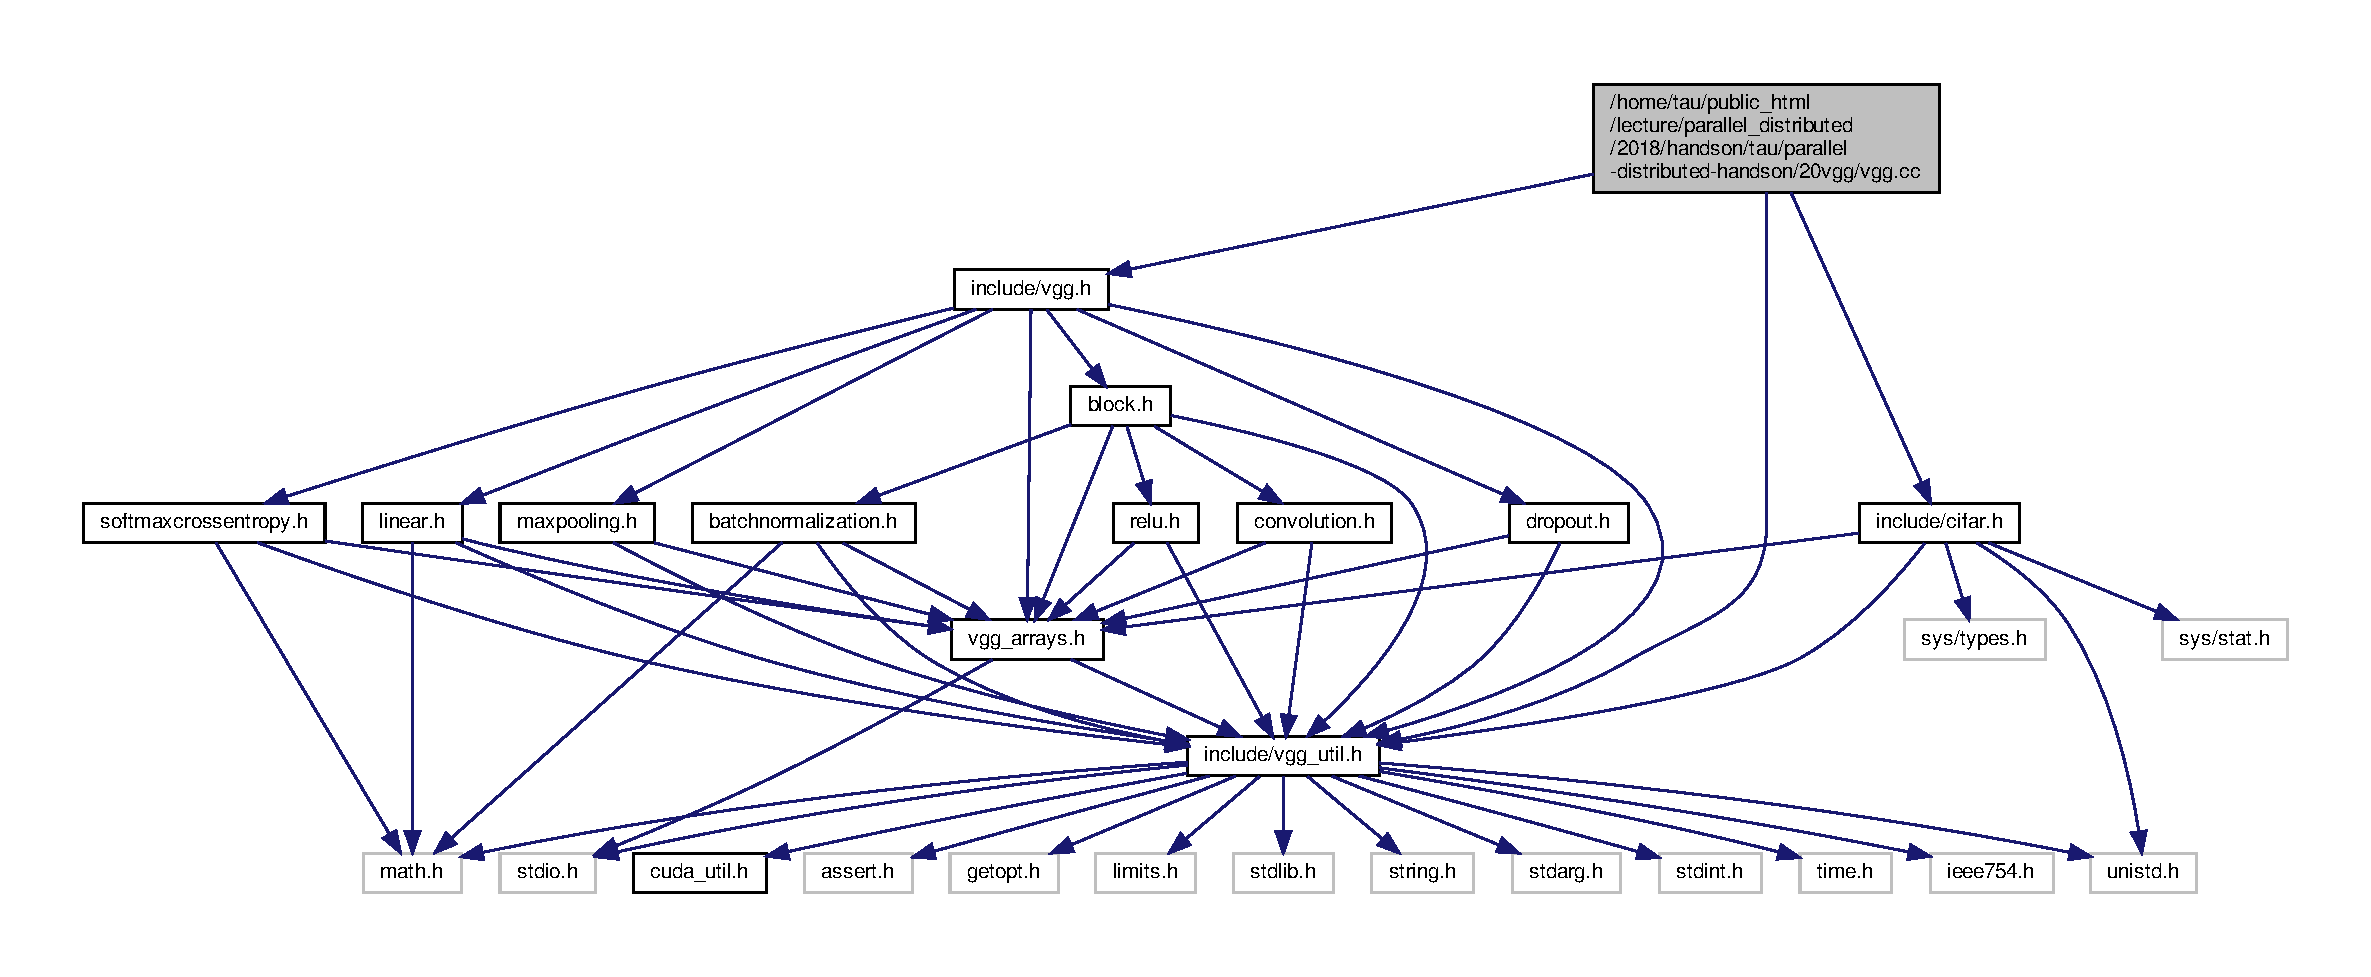
\includegraphics[width=350pt]{vgg_8cc__incl}
\end{center}
\end{figure}
\subsection*{Functions}
\begin{DoxyCompactItemize}
\item 
{\footnotesize template$<$idx\+\_\+t maxB, idx\+\_\+t C0, idx\+\_\+t H, idx\+\_\+t W, idx\+\_\+t K, idx\+\_\+t S, idx\+\_\+t C1, idx\+\_\+t nC$>$ }\\static \hyperlink{vgg__util_8h_a1082d08aaa761215ec83e7149f27ad16}{real} \hyperlink{vgg_8cc_a4b438057b926d7708dec390aa2948569}{train} (\hyperlink{structVGG}{V\+GG}$<$ maxB, C0, H, W, K, S, C1, nC $>$ $\ast$vgg, \hyperlink{structcifar10__dataset}{cifar10\+\_\+dataset}$<$ maxB, C0, H, W $>$ \&data, \hyperlink{vgg__util_8h_a8e93478a00e685bea5e6a3f617bf03a3}{idx\+\_\+t} B, long count)
\begin{DoxyCompactList}\small\item\em grab a mini batch (B training samples), forward, backward and update. \end{DoxyCompactList}\item 
{\footnotesize template$<$idx\+\_\+t maxB, idx\+\_\+t C0, idx\+\_\+t H, idx\+\_\+t W, idx\+\_\+t K, idx\+\_\+t S, idx\+\_\+t C1, idx\+\_\+t nC$>$ }\\static \hyperlink{vgg__util_8h_a1082d08aaa761215ec83e7149f27ad16}{real} \hyperlink{vgg_8cc_a04d52217a0a48fc133711ff5eb0153ca}{validate} (\hyperlink{structVGG}{V\+GG}$<$ maxB, C0, H, W, K, S, C1, nC $>$ $\ast$vgg, \hyperlink{structcifar10__dataset}{cifar10\+\_\+dataset}$<$ maxB, C0, H, W $>$ \&data, long count)
\begin{DoxyCompactList}\small\item\em forward compute B\+\_\+validate validation samples (taking several mini batches if necessary) \end{DoxyCompactList}\item 
int \hyperlink{vgg_8cc_a3c04138a5bfe5d72780bb7e82a18e627}{main} (int argc, char $\ast$$\ast$argv)
\begin{DoxyCompactList}\small\item\em main function of \hyperlink{structVGG}{V\+GG} \end{DoxyCompactList}\end{DoxyCompactItemize}


\subsection{Detailed Description}
--- a C++ implemention of \hyperlink{structVGG}{V\+GG} 

\subsection{Function Documentation}
\mbox{\Hypertarget{vgg_8cc_a3c04138a5bfe5d72780bb7e82a18e627}\label{vgg_8cc_a3c04138a5bfe5d72780bb7e82a18e627}} 
\index{vgg.\+cc@{vgg.\+cc}!main@{main}}
\index{main@{main}!vgg.\+cc@{vgg.\+cc}}
\subsubsection{\texorpdfstring{main()}{main()}}
{\footnotesize\ttfamily int main (\begin{DoxyParamCaption}\item[{int}]{argc,  }\item[{char $\ast$$\ast$}]{argv }\end{DoxyParamCaption})}



main function of \hyperlink{structVGG}{V\+GG} 

Train \hyperlink{structVGG}{V\+GG} network with data from the file specified by --cifar\+\_\+data/-\/d (default\+: cifar-\/10-\/batches-\/bin/data\+\_\+batch\+\_\+1.\+bin). If you want to use only a part of data, you can specify a range by --start\+\_\+data and --end\+\_\+data. e.\+g., --start Take a number of samples specified by --batch\+\_\+sz/-\/d samples at a time for training. Occasionally evaluate the network with validation data. \begin{DoxyReturn}{Returns}
the average loss of the validation data 
\end{DoxyReturn}
$<$ max batch size (constant)

$<$ true batch size ($<$= maxB)

$<$ input channels (R\+GB)

$<$ height of an image

$<$ width of an image

$<$ kernel size (K=1 -\/$>$ 3x3)

$<$ max pooling stride HxW -\/$>$ H/\+Sx\+W/S

$<$ channels of the last stage

$<$ number of classes \mbox{\Hypertarget{vgg_8cc_a4b438057b926d7708dec390aa2948569}\label{vgg_8cc_a4b438057b926d7708dec390aa2948569}} 
\index{vgg.\+cc@{vgg.\+cc}!train@{train}}
\index{train@{train}!vgg.\+cc@{vgg.\+cc}}
\subsubsection{\texorpdfstring{train()}{train()}}
{\footnotesize\ttfamily template$<$idx\+\_\+t maxB, idx\+\_\+t C0, idx\+\_\+t H, idx\+\_\+t W, idx\+\_\+t K, idx\+\_\+t S, idx\+\_\+t C1, idx\+\_\+t nC$>$ \\
static \hyperlink{vgg__util_8h_a1082d08aaa761215ec83e7149f27ad16}{real} train (\begin{DoxyParamCaption}\item[{\hyperlink{structVGG}{V\+GG}$<$ maxB, C0, H, W, K, S, C1, nC $>$ $\ast$}]{vgg,  }\item[{\hyperlink{structcifar10__dataset}{cifar10\+\_\+dataset}$<$ maxB, C0, H, W $>$ \&}]{data,  }\item[{\hyperlink{vgg__util_8h_a8e93478a00e685bea5e6a3f617bf03a3}{idx\+\_\+t}}]{B,  }\item[{long}]{count }\end{DoxyParamCaption})\hspace{0.3cm}{\ttfamily [static]}}



grab a mini batch (B training samples), forward, backward and update. 

\begin{DoxyReturn}{Returns}
the average loss of the mini batch. 
\end{DoxyReturn}
\mbox{\Hypertarget{vgg_8cc_a04d52217a0a48fc133711ff5eb0153ca}\label{vgg_8cc_a04d52217a0a48fc133711ff5eb0153ca}} 
\index{vgg.\+cc@{vgg.\+cc}!validate@{validate}}
\index{validate@{validate}!vgg.\+cc@{vgg.\+cc}}
\subsubsection{\texorpdfstring{validate()}{validate()}}
{\footnotesize\ttfamily template$<$idx\+\_\+t maxB, idx\+\_\+t C0, idx\+\_\+t H, idx\+\_\+t W, idx\+\_\+t K, idx\+\_\+t S, idx\+\_\+t C1, idx\+\_\+t nC$>$ \\
static \hyperlink{vgg__util_8h_a1082d08aaa761215ec83e7149f27ad16}{real} validate (\begin{DoxyParamCaption}\item[{\hyperlink{structVGG}{V\+GG}$<$ maxB, C0, H, W, K, S, C1, nC $>$ $\ast$}]{vgg,  }\item[{\hyperlink{structcifar10__dataset}{cifar10\+\_\+dataset}$<$ maxB, C0, H, W $>$ \&}]{data,  }\item[{long}]{count }\end{DoxyParamCaption})\hspace{0.3cm}{\ttfamily [static]}}



forward compute B\+\_\+validate validation samples (taking several mini batches if necessary) 

\begin{DoxyReturn}{Returns}
the average loss of the validation data 
\end{DoxyReturn}

%--- End generated contents ---

% Index
\backmatter
\newpage
\phantomsection
\clearemptydoublepage
\addcontentsline{toc}{chapter}{Index}
\printindex

\end{document}
